\documentclass[twoside]{book}

% Packages required by doxygen
\usepackage{fixltx2e}
\usepackage{calc}
\usepackage{doxygen}
\usepackage[export]{adjustbox} % also loads graphicx
\usepackage{graphicx}
\usepackage[utf8]{inputenc}
\usepackage{makeidx}
\usepackage{multicol}
\usepackage{multirow}
\PassOptionsToPackage{warn}{textcomp}
\usepackage{textcomp}
\usepackage[nointegrals]{wasysym}
\usepackage[table]{xcolor}

% Font selection
\usepackage[T1]{fontenc}
\usepackage[scaled=.90]{helvet}
\usepackage{courier}
\usepackage{amssymb}
\usepackage{sectsty}
\renewcommand{\familydefault}{\sfdefault}
\allsectionsfont{%
  \fontseries{bc}\selectfont%
  \color{darkgray}%
}
\renewcommand{\DoxyLabelFont}{%
  \fontseries{bc}\selectfont%
  \color{darkgray}%
}
\newcommand{\+}{\discretionary{\mbox{\scriptsize$\hookleftarrow$}}{}{}}

% Page & text layout
\usepackage{geometry}
\geometry{%
  a4paper,%
  top=2.5cm,%
  bottom=2.5cm,%
  left=2.5cm,%
  right=2.5cm%
}
\tolerance=750
\hfuzz=15pt
\hbadness=750
\setlength{\emergencystretch}{15pt}
\setlength{\parindent}{0cm}
\setlength{\parskip}{3ex plus 2ex minus 2ex}
\makeatletter
\renewcommand{\paragraph}{%
  \@startsection{paragraph}{4}{0ex}{-1.0ex}{1.0ex}{%
    \normalfont\normalsize\bfseries\SS@parafont%
  }%
}
\renewcommand{\subparagraph}{%
  \@startsection{subparagraph}{5}{0ex}{-1.0ex}{1.0ex}{%
    \normalfont\normalsize\bfseries\SS@subparafont%
  }%
}
\makeatother

% Headers & footers
\usepackage{fancyhdr}
\pagestyle{fancyplain}
\fancyhead[LE]{\fancyplain{}{\bfseries\thepage}}
\fancyhead[CE]{\fancyplain{}{}}
\fancyhead[RE]{\fancyplain{}{\bfseries\leftmark}}
\fancyhead[LO]{\fancyplain{}{\bfseries\rightmark}}
\fancyhead[CO]{\fancyplain{}{}}
\fancyhead[RO]{\fancyplain{}{\bfseries\thepage}}
\fancyfoot[LE]{\fancyplain{}{}}
\fancyfoot[CE]{\fancyplain{}{}}
\fancyfoot[RE]{\fancyplain{}{\bfseries\scriptsize Generated by Doxygen }}
\fancyfoot[LO]{\fancyplain{}{\bfseries\scriptsize Generated by Doxygen }}
\fancyfoot[CO]{\fancyplain{}{}}
\fancyfoot[RO]{\fancyplain{}{}}
\renewcommand{\footrulewidth}{0.4pt}
\renewcommand{\chaptermark}[1]{%
  \markboth{#1}{}%
}
\renewcommand{\sectionmark}[1]{%
  \markright{\thesection\ #1}%
}

% Indices & bibliography
\usepackage{natbib}
\usepackage[titles]{tocloft}
\setcounter{tocdepth}{3}
\setcounter{secnumdepth}{5}
\makeindex

% Hyperlinks (required, but should be loaded last)
\usepackage{ifpdf}
\ifpdf
  \usepackage[pdftex,pagebackref=true]{hyperref}
\else
  \usepackage[ps2pdf,pagebackref=true]{hyperref}
\fi
\hypersetup{%
  colorlinks=true,%
  linkcolor=blue,%
  citecolor=blue,%
  unicode%
}

% Custom commands
\newcommand{\clearemptydoublepage}{%
  \newpage{\pagestyle{empty}\cleardoublepage}%
}

\usepackage{caption}
\captionsetup{labelsep=space,justification=centering,font={bf},singlelinecheck=off,skip=4pt,position=top}

%===== C O N T E N T S =====

\begin{document}

% Titlepage & ToC
\hypersetup{pageanchor=false,
             bookmarksnumbered=true,
             pdfencoding=unicode
            }
\pagenumbering{alph}
\begin{titlepage}
\vspace*{7cm}
\begin{center}%
{\Large Eye\+Candy3D }\\
\vspace*{1cm}
{\large Generated by Doxygen 1.8.14}\\
\end{center}
\end{titlepage}
\clearemptydoublepage
\pagenumbering{roman}
\tableofcontents
\clearemptydoublepage
\pagenumbering{arabic}
\hypersetup{pageanchor=true}

%--- Begin generated contents ---
\chapter{Todo List}
\label{todo}
\Hypertarget{todo}

\begin{DoxyRefList}
\item[\label{todo__todo000003}%
\Hypertarget{todo__todo000003}%
Member \mbox{\hyperlink{classagui_1_1_open_g_l_font_a5cee06ae51d416cfb2997aa1ac7177ac}{agui\+:\+:Open\+G\+L\+Font\+:\+:get\+Text\+Width}} (const std\+::string \&text) const override]implement  
\item[\label{todo__todo000004}%
\Hypertarget{todo__todo000004}%
Member \mbox{\hyperlink{classagui_1_1_open_g_l_font_a6361880d5d7cf07935d548b77c2d354b}{agui\+:\+:Open\+G\+L\+Font\+:\+:reload}} (const std\+::string \&file\+Name, int height, Font\+Flags font\+Flags=F\+O\+N\+T\+\_\+\+D\+E\+F\+A\+U\+L\+T\+\_\+\+F\+L\+A\+GS, float border\+Width=0, agui\+::\+Color border\+Color=agui\+::\+Color()) override]implement  
\item[\label{todo__todo000002}%
\Hypertarget{todo__todo000002}%
Member \mbox{\hyperlink{classagui_1_1_open_g_l_font_a0b8b5c5bd6a8cda3767a3215c48a2e01}{agui\+:\+:Open\+G\+L\+Font\+:\+:set\+Font}} (\mbox{\hyperlink{classec_1_1_font_texture_atlas}{ec\+::\+Font\+Texture\+Atlas}} $\ast$font, const std\+::string \&path, bool auto\+Free=false)]implement  
\item[\label{todo__todo000005}%
\Hypertarget{todo__todo000005}%
Member \mbox{\hyperlink{classagui_1_1_open_g_l_graphics_ad0158ea89307d21c96cde0a47e982f72}{agui\+:\+:Open\+G\+L\+Graphics\+:\+:\+\_\+begin\+Paint}} () override]enable transparency, enable shader, set current context  
\item[\label{todo__todo000006}%
\Hypertarget{todo__todo000006}%
Member \mbox{\hyperlink{classagui_1_1_open_g_l_graphics_a744c073f057d938eec458a2517f5822a}{agui\+:\+:Open\+G\+L\+Graphics\+:\+:\+\_\+end\+Paint}} () override]disable transparency, disable shader  
\item[\label{todo__todo000007}%
\Hypertarget{todo__todo000007}%
Member \mbox{\hyperlink{classagui_1_1_open_g_l_image_acea75a4849d6e14c608bc93be52e20c4}{agui\+:\+:Open\+G\+L\+Image\+:\+:get\+Pixel}} (int x, int y) const override]implement  
\item[\label{todo__todo000008}%
\Hypertarget{todo__todo000008}%
Member \mbox{\hyperlink{classagui_1_1_open_g_l_image_a149afec919d0975af4fc48a078c183e2}{agui\+:\+:Open\+G\+L\+Image\+:\+:set\+Pixel}} (int x, int y, const Color \&color) override]implement  
\item[\label{todo__todo000009}%
\Hypertarget{todo__todo000009}%
Member \mbox{\hyperlink{classec__gui_1_1_g_u_i_controller_a3d9e413ddf78d41e929ec652c5409f3c}{ec\+\_\+gui\+:\+:G\+U\+I\+Controller\+:\+:Process\+Event}} (const \mbox{\hyperlink{structec_1_1_input_event}{ec\+::\+Input\+Event}} \&event) override]implement \mbox{\hyperlink{classec__gui_1_1_g_u_i_controller}{G\+U\+I\+Controller}} Process\+Event 
\end{DoxyRefList}
\chapter{Namespace Index}
\section{Namespace List}
Here is a list of all namespaces with brief descriptions\+:\begin{DoxyCompactList}
\item\contentsline{section}{\mbox{\hyperlink{namespaceagui}{agui}} }{\pageref{namespaceagui}}{}
\item\contentsline{section}{\mbox{\hyperlink{namespaceconf}{conf}} }{\pageref{namespaceconf}}{}
\item\contentsline{section}{\mbox{\hyperlink{namespaceconf__shader}{conf\+\_\+shader}} }{\pageref{namespaceconf__shader}}{}
\item\contentsline{section}{\mbox{\hyperlink{namespaceec}{ec}} }{\pageref{namespaceec}}{}
\end{DoxyCompactList}

\chapter{Hierarchical Index}
\section{Class Hierarchy}
This inheritance list is sorted roughly, but not completely, alphabetically\+:\begin{DoxyCompactList}
\item \contentsline{section}{ec\+:\+:Application}{\pageref{classec_1_1_application}}{}
\item \contentsline{section}{ec\+\_\+gui\+:\+:Bounds2D}{\pageref{classec__gui_1_1_bounds2_d}}{}
\item \contentsline{section}{ec\+:\+:Cursor}{\pageref{classec_1_1_cursor}}{}
\item \contentsline{section}{Cursor\+Provider}{\pageref{class_cursor_provider}}{}
\begin{DoxyCompactList}
\item \contentsline{section}{agui\+:\+:Open\+G\+L\+Cursor\+Provider}{\pageref{classagui_1_1_open_g_l_cursor_provider}}{}
\end{DoxyCompactList}
\item \contentsline{section}{ec\+:\+:Device\+Registry}{\pageref{classec_1_1_device_registry}}{}
\item \contentsline{section}{ec\+:\+:Display\+Event}{\pageref{structec_1_1_display_event}}{}
\item \contentsline{section}{ec\+:\+:Drawable}{\pageref{classec_1_1_drawable}}{}
\item \contentsline{section}{ec\+:\+:Drop\+Event}{\pageref{structec_1_1_drop_event}}{}
\item \contentsline{section}{ec\+:\+:Event\+Data}{\pageref{unionec_1_1_event_data}}{}
\item \contentsline{section}{ec\+:\+:Event\+System}{\pageref{classec_1_1_event_system}}{}
\item \contentsline{section}{utl\+:\+:File\+Logger}{\pageref{classutl_1_1_file_logger}}{}
\item \contentsline{section}{Font}{\pageref{class_font}}{}
\begin{DoxyCompactList}
\item \contentsline{section}{agui\+:\+:Open\+G\+L\+Font}{\pageref{classagui_1_1_open_g_l_font}}{}
\end{DoxyCompactList}
\item \contentsline{section}{ec\+:\+:Font\+Character}{\pageref{structec_1_1_font_character}}{}
\item \contentsline{section}{Font\+Loader}{\pageref{class_font_loader}}{}
\begin{DoxyCompactList}
\item \contentsline{section}{agui\+:\+:Open\+G\+L\+Font\+Loader}{\pageref{classagui_1_1_open_g_l_font_loader}}{}
\end{DoxyCompactList}
\item \contentsline{section}{ec\+:\+:Font\+Texture\+Atlas}{\pageref{classec_1_1_font_texture_atlas}}{}
\item \contentsline{section}{ec\+:\+:Frame}{\pageref{classec_1_1_frame}}{}
\item \contentsline{section}{ec\+:\+:Freetype}{\pageref{classec_1_1_freetype}}{}
\item \contentsline{section}{ec\+:\+:Geometry\+Data}{\pageref{structec_1_1_geometry_data}}{}
\item \contentsline{section}{Graphics}{\pageref{class_graphics}}{}
\begin{DoxyCompactList}
\item \contentsline{section}{agui\+:\+:Open\+G\+L\+Graphics}{\pageref{classagui_1_1_open_g_l_graphics}}{}
\end{DoxyCompactList}
\item \contentsline{section}{ec\+\_\+gui\+:\+:Gui}{\pageref{classec__gui_1_1_gui}}{}
\item \contentsline{section}{ec\+\_\+gui\+:\+:Gui\+Model}{\pageref{classec__gui_1_1_gui_model}}{}
\item \contentsline{section}{ec\+\_\+gui\+:\+:Gui\+Renderer}{\pageref{classec__gui_1_1_gui_renderer}}{}
\item \contentsline{section}{ec\+\_\+gui\+:\+:Gui\+Rendering\+Context}{\pageref{classec__gui_1_1_gui_rendering_context}}{}
\item \contentsline{section}{ec\+\_\+gui\+:\+:Gui\+Rendering\+Parameter\+List}{\pageref{structec__gui_1_1_gui_rendering_parameter_list}}{}
\item \contentsline{section}{ec\+\_\+gui\+:\+:Gui\+System}{\pageref{classec__gui_1_1_gui_system}}{}
\item \contentsline{section}{ec\+:\+:I\+Geometry\+Access}{\pageref{classec_1_1_i_geometry_access}}{}
\begin{DoxyCompactList}
\item \contentsline{section}{ec\+:\+:Geometry}{\pageref{classec_1_1_geometry}}{}
\begin{DoxyCompactList}
\item \contentsline{section}{ec\+:\+:Dynamic\+Geometry}{\pageref{classec_1_1_dynamic_geometry}}{}
\begin{DoxyCompactList}
\item \contentsline{section}{ec\+:\+:Dynamic\+Line\+Geometry}{\pageref{classec_1_1_dynamic_line_geometry}}{}
\end{DoxyCompactList}
\item \contentsline{section}{ec\+:\+:Static\+Geometry}{\pageref{classec_1_1_static_geometry}}{}
\begin{DoxyCompactList}
\item \contentsline{section}{ec\+:\+:Cube\+Geometry}{\pageref{classec_1_1_cube_geometry}}{}
\item \contentsline{section}{ec\+:\+:Rectangle\+Mesh}{\pageref{classec_1_1_rectangle_mesh}}{}
\item \contentsline{section}{ec\+:\+:Sphere\+Geometry}{\pageref{classec_1_1_sphere_geometry}}{}
\end{DoxyCompactList}
\end{DoxyCompactList}
\item \contentsline{section}{ec\+:\+:Spring\+Geometry}{\pageref{classec_1_1_spring_geometry}}{}
\end{DoxyCompactList}
\item \contentsline{section}{Image}{\pageref{class_image}}{}
\begin{DoxyCompactList}
\item \contentsline{section}{agui\+:\+:Open\+G\+L\+Image}{\pageref{classagui_1_1_open_g_l_image}}{}
\end{DoxyCompactList}
\item \contentsline{section}{Image\+Loader}{\pageref{class_image_loader}}{}
\begin{DoxyCompactList}
\item \contentsline{section}{agui\+:\+:Open\+G\+L\+Image\+Loader}{\pageref{classagui_1_1_open_g_l_image_loader}}{}
\end{DoxyCompactList}
\item \contentsline{section}{Input}{\pageref{class_input}}{}
\begin{DoxyCompactList}
\item \contentsline{section}{agui\+:\+:Open\+G\+L\+Input}{\pageref{classagui_1_1_open_g_l_input}}{}
\end{DoxyCompactList}
\item \contentsline{section}{ec\+:\+:Input\+Event}{\pageref{structec_1_1_input_event}}{}
\item \contentsline{section}{ec\+:\+:Input\+Listener}{\pageref{classec_1_1_input_listener}}{}
\begin{DoxyCompactList}
\item \contentsline{section}{agui\+:\+:Open\+G\+L\+Input}{\pageref{classagui_1_1_open_g_l_input}}{}
\item \contentsline{section}{ec\+:\+:Camera\+Controller}{\pageref{classec_1_1_camera_controller}}{}
\item \contentsline{section}{ec\+:\+:Scene\+Controller}{\pageref{classec_1_1_scene_controller}}{}
\item \contentsline{section}{ec\+\_\+gui\+:\+:Gui\+Controller}{\pageref{classec__gui_1_1_gui_controller}}{}
\end{DoxyCompactList}
\item \contentsline{section}{ec\+:\+:Input\+Observable}{\pageref{classec_1_1_input_observable}}{}
\item \contentsline{section}{ec\+:\+:Joystick\+Event}{\pageref{structec_1_1_joystick_event}}{}
\item \contentsline{section}{ec\+:\+:Keyboard}{\pageref{classec_1_1_keyboard}}{}
\item \contentsline{section}{ec\+:\+:Keyboard\+Event}{\pageref{structec_1_1_keyboard_event}}{}
\item \contentsline{section}{ec\+:\+:Material}{\pageref{classec_1_1_material}}{}
\item \contentsline{section}{ec\+:\+:Mouse}{\pageref{classec_1_1_mouse}}{}
\item \contentsline{section}{ec\+:\+:Mouse\+Event}{\pageref{structec_1_1_mouse_event}}{}
\item \contentsline{section}{utl\+:\+:Profiling\+Data}{\pageref{structutl_1_1_profiling_data}}{}
\item \contentsline{section}{utl\+:\+:Random}{\pageref{classutl_1_1_random}}{}
\item \contentsline{section}{ec\+:\+:Renderer}{\pageref{classec_1_1_renderer}}{}
\item \contentsline{section}{ec\+:\+:Resource\+Registry$<$ Resource $>$}{\pageref{classec_1_1_resource_registry}}{}
\item \contentsline{section}{ec\+:\+:Resource\+Registry$<$ ec\+:\+:Drawable $>$}{\pageref{classec_1_1_resource_registry}}{}
\item \contentsline{section}{ec\+:\+:Resource\+Registry$<$ ec\+:\+:Geometry $>$}{\pageref{classec_1_1_resource_registry}}{}
\item \contentsline{section}{ec\+:\+:Resource\+Registry$<$ ec\+:\+:Material $>$}{\pageref{classec_1_1_resource_registry}}{}
\item \contentsline{section}{ec\+:\+:Resource\+Registry$<$ ec\+:\+:Texture $>$}{\pageref{classec_1_1_resource_registry}}{}
\item \contentsline{section}{ec\+:\+:Scene}{\pageref{classec_1_1_scene}}{}
\item \contentsline{section}{ec\+:\+:Scene\+Renderer}{\pageref{classec_1_1_scene_renderer}}{}
\item \contentsline{section}{ec\+:\+:Scene\+System}{\pageref{classec_1_1_scene_system}}{}
\item \contentsline{section}{ec\+:\+:Shader}{\pageref{classec_1_1_shader}}{}
\item \contentsline{section}{ec\+:\+:Shader\+Manager}{\pageref{classec_1_1_shader_manager}}{}
\item \contentsline{section}{ec\+:\+:Texture}{\pageref{classec_1_1_texture}}{}
\item \contentsline{section}{ec\+:\+:Texture\+Types}{\pageref{structec_1_1_texture_types}}{}
\item \contentsline{section}{ec\+\_\+gui\+:\+:Theme}{\pageref{classec__gui_1_1_theme}}{}
\item \contentsline{section}{ec\+:\+:Timer}{\pageref{classec_1_1_timer}}{}
\item \contentsline{section}{ec\+:\+:Transform3D}{\pageref{classec_1_1_transform3_d}}{}
\begin{DoxyCompactList}
\item \contentsline{section}{ec\+:\+:Node}{\pageref{classec_1_1_node}}{}
\begin{DoxyCompactList}
\item \contentsline{section}{ec\+:\+:Camera}{\pageref{classec_1_1_camera}}{}
\end{DoxyCompactList}
\end{DoxyCompactList}
\item \contentsline{section}{ec\+:\+:Vertex}{\pageref{structec_1_1_vertex}}{}
\item \contentsline{section}{ec\+:\+:Viewport}{\pageref{classec_1_1_viewport}}{}
\item \contentsline{section}{ec\+\_\+gui\+:\+:Widget}{\pageref{classec__gui_1_1_widget}}{}
\begin{DoxyCompactList}
\item \contentsline{section}{ec\+\_\+gui\+:\+:Button}{\pageref{classec__gui_1_1_button}}{}
\item \contentsline{section}{ec\+\_\+gui\+:\+:Checkbox}{\pageref{classec__gui_1_1_checkbox}}{}
\item \contentsline{section}{ec\+\_\+gui\+:\+:Horizontal\+List}{\pageref{classec__gui_1_1_horizontal_list}}{}
\item \contentsline{section}{ec\+\_\+gui\+:\+:Radio\+Button}{\pageref{classec__gui_1_1_radio_button}}{}
\item \contentsline{section}{ec\+\_\+gui\+:\+:Screen}{\pageref{classec__gui_1_1_screen}}{}
\item \contentsline{section}{ec\+\_\+gui\+:\+:Slot$<$ Widget\+Type $>$}{\pageref{classec__gui_1_1_slot}}{}
\item \contentsline{section}{ec\+\_\+gui\+:\+:Slot\+Pair$<$ First\+Widget, Second\+Widget $>$}{\pageref{classec__gui_1_1_slot_pair}}{}
\item \contentsline{section}{ec\+\_\+gui\+:\+:Text}{\pageref{classec__gui_1_1_text}}{}
\begin{DoxyCompactList}
\item \contentsline{section}{ec\+\_\+gui\+:\+:Text\+Field}{\pageref{classec__gui_1_1_text_field}}{}
\end{DoxyCompactList}
\item \contentsline{section}{ec\+\_\+gui\+:\+:Vertical\+List}{\pageref{classec__gui_1_1_vertical_list}}{}
\item \contentsline{section}{ec\+\_\+gui\+:\+:Window}{\pageref{classec__gui_1_1_window}}{}
\end{DoxyCompactList}
\item \contentsline{section}{ec\+:\+:Window}{\pageref{classec_1_1_window}}{}
\end{DoxyCompactList}

\chapter{Class Index}
\section{Class List}
Here are the classes, structs, unions and interfaces with brief descriptions\+:\begin{DoxyCompactList}
\item\contentsline{section}{\mbox{\hyperlink{classec_1_1_application}{ec\+::\+Application}} }{\pageref{classec_1_1_application}}{}
\item\contentsline{section}{\mbox{\hyperlink{classec_1_1_camera}{ec\+::\+Camera}} \\*A camera encapsulates a view and a projection matrix. It is used to render the related scene. It contains a viewport, which defines the area of the render target the scene should be rendered into }{\pageref{classec_1_1_camera}}{}
\item\contentsline{section}{\mbox{\hyperlink{classec_1_1_camera_controller}{ec\+::\+Camera\+Controller}} }{\pageref{classec_1_1_camera_controller}}{}
\item\contentsline{section}{\mbox{\hyperlink{classec_1_1_circle_geometry}{ec\+::\+Circle\+Geometry}} \\*Concrete static geometry that represents a circle }{\pageref{classec_1_1_circle_geometry}}{}
\item\contentsline{section}{\mbox{\hyperlink{classec_1_1_cube_geometry}{ec\+::\+Cube\+Geometry}} \\*Concrete static geometry that represents a cube }{\pageref{classec_1_1_cube_geometry}}{}
\item\contentsline{section}{\mbox{\hyperlink{classec_1_1_cursor}{ec\+::\+Cursor}} \\*A cursor describes the bitmap used for a cursor }{\pageref{classec_1_1_cursor}}{}
\item\contentsline{section}{\mbox{\hyperlink{classec_1_1_cylinder_geometry}{ec\+::\+Cylinder\+Geometry}} \\*Kind of static geometry that represents a cylinder }{\pageref{classec_1_1_cylinder_geometry}}{}
\item\contentsline{section}{\mbox{\hyperlink{classec_1_1_device_registry}{ec\+::\+Device\+Registry}} \\*Stores all different kinds of input devices }{\pageref{classec_1_1_device_registry}}{}
\item\contentsline{section}{\mbox{\hyperlink{classec_1_1_directional_light}{ec\+::\+Directional\+Light}} \\*A light source that emits light in a given direction independently of its position }{\pageref{classec_1_1_directional_light}}{}
\item\contentsline{section}{\mbox{\hyperlink{structec_1_1_display_event}{ec\+::\+Display\+Event}} \\*An event sent by the window }{\pageref{structec_1_1_display_event}}{}
\item\contentsline{section}{\mbox{\hyperlink{classec_1_1_drawable}{ec\+::\+Drawable}} \\*Core class for rendering geometry data with a certain material and shader }{\pageref{classec_1_1_drawable}}{}
\item\contentsline{section}{\mbox{\hyperlink{structec_1_1_drop_event}{ec\+::\+Drop\+Event}} \\*An event generated by dragging and dropping links into a window }{\pageref{structec_1_1_drop_event}}{}
\item\contentsline{section}{\mbox{\hyperlink{classec_1_1_dynamic_geometry}{ec\+::\+Dynamic\+Geometry}} \\*Kind of geometry that can be changed for every rendering }{\pageref{classec_1_1_dynamic_geometry}}{}
\item\contentsline{section}{\mbox{\hyperlink{classec_1_1_dynamic_line_geometry}{ec\+::\+Dynamic\+Line\+Geometry}} \\*Line geometry that adapts to a given start and end point }{\pageref{classec_1_1_dynamic_line_geometry}}{}
\item\contentsline{section}{\mbox{\hyperlink{unionec_1_1_event_data}{ec\+::\+Event\+Data}} \\*Holds the actual data of an event. Only one event can be active at a time }{\pageref{unionec_1_1_event_data}}{}
\item\contentsline{section}{\mbox{\hyperlink{classec_1_1_event_system}{ec\+::\+Event\+System}} \\*Responsible for the distribution of input events }{\pageref{classec_1_1_event_system}}{}
\item\contentsline{section}{\mbox{\hyperlink{classec_1_1_file_system}{ec\+::\+File\+System}} \\*Static class, which contains utility file system functions }{\pageref{classec_1_1_file_system}}{}
\item\contentsline{section}{\mbox{\hyperlink{structec_1_1_font_character}{ec\+::\+Font\+Character}} \\*A font character holds information about a specific character of a specific font }{\pageref{structec_1_1_font_character}}{}
\item\contentsline{section}{\mbox{\hyperlink{classec_1_1_font_texture_atlas}{ec\+::\+Font\+Texture\+Atlas}} \\*Saves all font characters of a specific font. Font characters will be saved on a single texture, so it can be used for rendering text }{\pageref{classec_1_1_font_texture_atlas}}{}
\item\contentsline{section}{\mbox{\hyperlink{classec_1_1_frame}{ec\+::\+Frame}} \\*A \mbox{\hyperlink{classec_1_1_frame}{Frame}} is a collection of cameras. The order in, which these cameras are stored, determines the order in which will be rendered }{\pageref{classec_1_1_frame}}{}
\item\contentsline{section}{\mbox{\hyperlink{classec_1_1_freetype}{ec\+::\+Freetype}} }{\pageref{classec_1_1_freetype}}{}
\item\contentsline{section}{\mbox{\hyperlink{classec_1_1_generic_action_listener}{ec\+::\+Generic\+Action\+Listener}} \\*Generic gui listener that can handle Action\+Events }{\pageref{classec_1_1_generic_action_listener}}{}
\item\contentsline{section}{\mbox{\hyperlink{classec_1_1_generic_button_listener}{ec\+::\+Generic\+Button\+Listener}} \\*Generic gui listener that can handle events by Button widgets }{\pageref{classec_1_1_generic_button_listener}}{}
\item\contentsline{section}{\mbox{\hyperlink{classec_1_1_generic_check_box_listener}{ec\+::\+Generic\+Check\+Box\+Listener}} \\*Generic gui listener that can handle events by Check\+Box widgets }{\pageref{classec_1_1_generic_check_box_listener}}{}
\item\contentsline{section}{\mbox{\hyperlink{classec_1_1_generic_drop_down_listener}{ec\+::\+Generic\+Drop\+Down\+Listener}} \\*Generic gui listener that can handle events by Drop\+Down widgets }{\pageref{classec_1_1_generic_drop_down_listener}}{}
\item\contentsline{section}{\mbox{\hyperlink{classec_1_1_generic_frame_listener}{ec\+::\+Generic\+Frame\+Listener}} \\*Generic gui listener that can handle events by \mbox{\hyperlink{classec_1_1_frame}{Frame}} widgets }{\pageref{classec_1_1_generic_frame_listener}}{}
\item\contentsline{section}{\mbox{\hyperlink{classec_1_1_generic_h_scroll_bar_listener}{ec\+::\+Generic\+H\+Scroll\+Bar\+Listener}} \\*Generic gui listener that can handle events by H\+Scrollbar widgets }{\pageref{classec_1_1_generic_h_scroll_bar_listener}}{}
\item\contentsline{section}{\mbox{\hyperlink{classec_1_1_generic_label_listener}{ec\+::\+Generic\+Label\+Listener}} \\*Generic gui listener that can handle events by Label widgets }{\pageref{classec_1_1_generic_label_listener}}{}
\item\contentsline{section}{\mbox{\hyperlink{classec_1_1_generic_list_box_listener}{ec\+::\+Generic\+List\+Box\+Listener}} \\*Generic gui listener that can handle events by List\+Box widgets }{\pageref{classec_1_1_generic_list_box_listener}}{}
\item\contentsline{section}{\mbox{\hyperlink{classec_1_1_generic_radio_button_listener}{ec\+::\+Generic\+Radio\+Button\+Listener}} \\*Generic gui listener that can handle events by Radio\+Button widgets }{\pageref{classec_1_1_generic_radio_button_listener}}{}
\item\contentsline{section}{\mbox{\hyperlink{classec_1_1_generic_slider_listener}{ec\+::\+Generic\+Slider\+Listener}} \\*Generic gui listener that can handle events by Slider widgets }{\pageref{classec_1_1_generic_slider_listener}}{}
\item\contentsline{section}{\mbox{\hyperlink{classec_1_1_generic_tabbed_pane_listener}{ec\+::\+Generic\+Tabbed\+Pane\+Listener}} \\*Generic gui listener that can handle events by Tabbed\+Pane widgets }{\pageref{classec_1_1_generic_tabbed_pane_listener}}{}
\item\contentsline{section}{\mbox{\hyperlink{classec_1_1_generic_text_box_listener}{ec\+::\+Generic\+Text\+Box\+Listener}} \\*Generic gui listener that can handle events by Text\+Box widgets }{\pageref{classec_1_1_generic_text_box_listener}}{}
\item\contentsline{section}{\mbox{\hyperlink{classec_1_1_generic_text_field_listener}{ec\+::\+Generic\+Text\+Field\+Listener}} \\*Generic gui listener that can handle events by Text\+Field widgets }{\pageref{classec_1_1_generic_text_field_listener}}{}
\item\contentsline{section}{\mbox{\hyperlink{classec_1_1_generic_v_scroll_bar_listener}{ec\+::\+Generic\+V\+Scroll\+Bar\+Listener}} \\*Generic gui listener that can handle events by V\+Scroll\+Bar widgets }{\pageref{classec_1_1_generic_v_scroll_bar_listener}}{}
\item\contentsline{section}{\mbox{\hyperlink{classec_1_1_generic_widget_listener}{ec\+::\+Generic\+Widget\+Listener}} \\*Generic gui listener that can handle events by widgets }{\pageref{classec_1_1_generic_widget_listener}}{}
\item\contentsline{section}{\mbox{\hyperlink{classec_1_1_geometry}{ec\+::\+Geometry}} \\*\mbox{\hyperlink{classec_1_1_geometry}{Geometry}} }{\pageref{classec_1_1_geometry}}{}
\item\contentsline{section}{\mbox{\hyperlink{classec_1_1_geometry_data}{ec\+::\+Geometry\+Data}} \\*Encapsulates vertex and index data and knows how to create, update and delete Open\+GL buffers }{\pageref{classec_1_1_geometry_data}}{}
\item\contentsline{section}{\mbox{\hyperlink{classec_1_1_gui_primitive_renderer}{ec\+::\+Gui\+Primitive\+Renderer}} }{\pageref{classec_1_1_gui_primitive_renderer}}{}
\item\contentsline{section}{\mbox{\hyperlink{structec_1_1_gui_render_context}{ec\+::\+Gui\+Render\+Context}} }{\pageref{structec_1_1_gui_render_context}}{}
\item\contentsline{section}{\mbox{\hyperlink{classec_1_1_gui_renderer}{ec\+::\+Gui\+Renderer}} }{\pageref{classec_1_1_gui_renderer}}{}
\item\contentsline{section}{\mbox{\hyperlink{structec_1_1_gui_shader_info_object}{ec\+::\+Gui\+Shader\+Info\+Object}} }{\pageref{structec_1_1_gui_shader_info_object}}{}
\item\contentsline{section}{\mbox{\hyperlink{classec_1_1_gui_system}{ec\+::\+Gui\+System}} }{\pageref{classec_1_1_gui_system}}{}
\item\contentsline{section}{\mbox{\hyperlink{classec_1_1_i_geometry_access}{ec\+::\+I\+Geometry\+Access}} \\*Base class for all kinds of geometry }{\pageref{classec_1_1_i_geometry_access}}{}
\item\contentsline{section}{\mbox{\hyperlink{structec_1_1_input_event}{ec\+::\+Input\+Event}} \\*Group all input events to make transfer easy and save memory by only holding the event, which is currently active }{\pageref{structec_1_1_input_event}}{}
\item\contentsline{section}{\mbox{\hyperlink{classec_1_1_input_listener}{ec\+::\+Input\+Listener}} \\*An \mbox{\hyperlink{classec_1_1_input_listener}{Input\+Listener}} can react on incoming events. It can either be used as a base class or be filled with callbacks }{\pageref{classec_1_1_input_listener}}{}
\item\contentsline{section}{\mbox{\hyperlink{classec_1_1_input_observable}{ec\+::\+Input\+Observable}} \\*Input\+Observables inform Input\+Listeners about Input\+Events }{\pageref{classec_1_1_input_observable}}{}
\item\contentsline{section}{\mbox{\hyperlink{structec_1_1_joystick_event}{ec\+::\+Joystick\+Event}} \\*An event generated by joystick interaction }{\pageref{structec_1_1_joystick_event}}{}
\item\contentsline{section}{\mbox{\hyperlink{classec_1_1_keyboard}{ec\+::\+Keyboard}} \\*Representation of a physical keyboard }{\pageref{classec_1_1_keyboard}}{}
\item\contentsline{section}{\mbox{\hyperlink{structec_1_1_keyboard_event}{ec\+::\+Keyboard\+Event}} \\*An event generated by keyboard interaction }{\pageref{structec_1_1_keyboard_event}}{}
\item\contentsline{section}{\mbox{\hyperlink{classec_1_1_light}{ec\+::\+Light}} \\*Abstract light source }{\pageref{classec_1_1_light}}{}
\item\contentsline{section}{\mbox{\hyperlink{classec_1_1_light_system}{ec\+::\+Light\+System}} \\*Contains a collection of different light sources }{\pageref{classec_1_1_light_system}}{}
\item\contentsline{section}{\mbox{\hyperlink{classec_1_1_line_geometry}{ec\+::\+Line\+Geometry}} \\*Describes the geometry of a single line }{\pageref{classec_1_1_line_geometry}}{}
\item\contentsline{section}{\mbox{\hyperlink{classec_1_1_line_geometry_factory}{ec\+::\+Line\+Geometry\+Factory}} \\*Create geometries, which are made out of multiple lines }{\pageref{classec_1_1_line_geometry_factory}}{}
\item\contentsline{section}{\mbox{\hyperlink{classec_1_1_line_strip_geometry}{ec\+::\+Line\+Strip\+Geometry}} \\*Describes the geometry of a line strip }{\pageref{classec_1_1_line_strip_geometry}}{}
\item\contentsline{section}{\mbox{\hyperlink{classec_1_1_logger}{ec\+::\+Logger}} \\*Log messages to console and create log files }{\pageref{classec_1_1_logger}}{}
\item\contentsline{section}{\mbox{\hyperlink{classec_1_1_material}{ec\+::\+Material}} \\*A material contains all relevant information to color an object }{\pageref{classec_1_1_material}}{}
\item\contentsline{section}{\mbox{\hyperlink{classec_1_1_mini_agui}{ec\+::\+Mini\+Agui}} }{\pageref{classec_1_1_mini_agui}}{}
\item\contentsline{section}{\mbox{\hyperlink{classec_1_1_mouse}{ec\+::\+Mouse}} \\*Represents a physical mouse }{\pageref{classec_1_1_mouse}}{}
\item\contentsline{section}{\mbox{\hyperlink{structec_1_1_mouse_event}{ec\+::\+Mouse\+Event}} \\*An event generated by mouse interaction }{\pageref{structec_1_1_mouse_event}}{}
\item\contentsline{section}{\mbox{\hyperlink{classec_1_1_node}{ec\+::\+Node}} \\*Nodes make up the scene graph. They represent a directed acyclic graph }{\pageref{classec_1_1_node}}{}
\item\contentsline{section}{\mbox{\hyperlink{classec_1_1_omni_light}{ec\+::\+Omni\+Light}} \\*Ambient lighting that acts everywhere }{\pageref{classec_1_1_omni_light}}{}
\item\contentsline{section}{\mbox{\hyperlink{classec_1_1_open_g_l_cursor_provider}{ec\+::\+Open\+G\+L\+Cursor\+Provider}} }{\pageref{classec_1_1_open_g_l_cursor_provider}}{}
\item\contentsline{section}{\mbox{\hyperlink{classec_1_1_open_g_l_font}{ec\+::\+Open\+G\+L\+Font}} }{\pageref{classec_1_1_open_g_l_font}}{}
\item\contentsline{section}{\mbox{\hyperlink{classec_1_1_open_g_l_font_loader}{ec\+::\+Open\+G\+L\+Font\+Loader}} }{\pageref{classec_1_1_open_g_l_font_loader}}{}
\item\contentsline{section}{\mbox{\hyperlink{classec_1_1_open_g_l_graphics}{ec\+::\+Open\+G\+L\+Graphics}} }{\pageref{classec_1_1_open_g_l_graphics}}{}
\item\contentsline{section}{\mbox{\hyperlink{classec_1_1_open_g_l_image}{ec\+::\+Open\+G\+L\+Image}} }{\pageref{classec_1_1_open_g_l_image}}{}
\item\contentsline{section}{\mbox{\hyperlink{classec_1_1_open_g_l_image_loader}{ec\+::\+Open\+G\+L\+Image\+Loader}} }{\pageref{classec_1_1_open_g_l_image_loader}}{}
\item\contentsline{section}{\mbox{\hyperlink{classec_1_1_open_g_l_input}{ec\+::\+Open\+G\+L\+Input}} }{\pageref{classec_1_1_open_g_l_input}}{}
\item\contentsline{section}{\mbox{\hyperlink{classec_1_1_point_light}{ec\+::\+Point\+Light}} \\*\mbox{\hyperlink{classec_1_1_light}{Light}} source, which emits light omnidirectional from a given position }{\pageref{classec_1_1_point_light}}{}
\item\contentsline{section}{\mbox{\hyperlink{structec_1_1_profiling_data}{ec\+::\+Profiling\+Data}} }{\pageref{structec_1_1_profiling_data}}{}
\item\contentsline{section}{\mbox{\hyperlink{classec_1_1_random}{ec\+::\+Random}} }{\pageref{classec_1_1_random}}{}
\item\contentsline{section}{\mbox{\hyperlink{classec_1_1_rectangle_geometry}{ec\+::\+Rectangle\+Geometry}} \\*\mbox{\hyperlink{classec_1_1_geometry}{Geometry}} that represents a filled rectangle }{\pageref{classec_1_1_rectangle_geometry}}{}
\item\contentsline{section}{\mbox{\hyperlink{classec_1_1_renderer}{ec\+::\+Renderer}} \\*A \mbox{\hyperlink{classec_1_1_renderer}{Renderer}} is responsible for rendering storing and using scene renderers }{\pageref{classec_1_1_renderer}}{}
\item\contentsline{section}{\mbox{\hyperlink{classec_1_1_resource_registry}{ec\+::\+Resource\+Registry$<$ Resource\+\_\+\+Type, Key\+\_\+\+Type $>$}} \\*Templated registry that stores key value pairs }{\pageref{classec_1_1_resource_registry}}{}
\item\contentsline{section}{\mbox{\hyperlink{classec_1_1_scene}{ec\+::\+Scene}} \\*A scene enables an easy switching of root nodes }{\pageref{classec_1_1_scene}}{}
\item\contentsline{section}{\mbox{\hyperlink{classec_1_1_scene_controller}{ec\+::\+Scene\+Controller}} \\*Specialized \mbox{\hyperlink{classec_1_1_input_listener}{Input\+Listener}} for controlling a scene }{\pageref{classec_1_1_scene_controller}}{}
\item\contentsline{section}{\mbox{\hyperlink{classec_1_1_scene_renderer}{ec\+::\+Scene\+Renderer}} }{\pageref{classec_1_1_scene_renderer}}{}
\item\contentsline{section}{\mbox{\hyperlink{classec_1_1_scene_system}{ec\+::\+Scene\+System}} }{\pageref{classec_1_1_scene_system}}{}
\item\contentsline{section}{\mbox{\hyperlink{classec_1_1_shader}{ec\+::\+Shader}} \\*Bundles vertex, fragment shader, geometry, tessellation control and tessellation evaluation shaders. \mbox{\hyperlink{classec_1_1_geometry}{Geometry}} and tessellation shaders are optional }{\pageref{classec_1_1_shader}}{}
\item\contentsline{section}{\mbox{\hyperlink{classec_1_1_shader_manager}{ec\+::\+Shader\+Manager}} }{\pageref{classec_1_1_shader_manager}}{}
\item\contentsline{section}{\mbox{\hyperlink{classec_1_1_shader_timed}{ec\+::\+Shader\+Timed}} }{\pageref{classec_1_1_shader_timed}}{}
\item\contentsline{section}{\mbox{\hyperlink{classec_1_1_sphere_geometry}{ec\+::\+Sphere\+Geometry}} \\*\mbox{\hyperlink{classec_1_1_geometry}{Geometry}} that represents a sphere }{\pageref{classec_1_1_sphere_geometry}}{}
\item\contentsline{section}{\mbox{\hyperlink{classec_1_1_spot_light}{ec\+::\+Spot\+Light}} \\*\mbox{\hyperlink{classec_1_1_light}{Light}} source with a direction and a conical shape }{\pageref{classec_1_1_spot_light}}{}
\item\contentsline{section}{\mbox{\hyperlink{classec_1_1_spring_geometry}{ec\+::\+Spring\+Geometry}} }{\pageref{classec_1_1_spring_geometry}}{}
\item\contentsline{section}{\mbox{\hyperlink{classec_1_1_static_geometry}{ec\+::\+Static\+Geometry}} \\*\mbox{\hyperlink{classec_1_1_geometry}{Geometry}} that does not change itself over time }{\pageref{classec_1_1_static_geometry}}{}
\item\contentsline{section}{\mbox{\hyperlink{classec_1_1_system_time}{ec\+::\+System\+Time}} }{\pageref{classec_1_1_system_time}}{}
\item\contentsline{section}{\mbox{\hyperlink{classec_1_1_texture}{ec\+::\+Texture}} \\*Create and destroy textures on the G\+PU and enable them for Open\+GL }{\pageref{classec_1_1_texture}}{}
\item\contentsline{section}{\mbox{\hyperlink{structec_1_1_texture_types}{ec\+::\+Texture\+Types}} \\*Encapsulates texture specific structures }{\pageref{structec_1_1_texture_types}}{}
\item\contentsline{section}{\mbox{\hyperlink{classec_1_1_timer}{ec\+::\+Timer}} }{\pageref{classec_1_1_timer}}{}
\item\contentsline{section}{\mbox{\hyperlink{classec_1_1_transform3_d}{ec\+::\+Transform3D}} \\*A transformation in 3D space }{\pageref{classec_1_1_transform3_d}}{}
\item\contentsline{section}{\mbox{\hyperlink{structec_1_1_vertex}{ec\+::\+Vertex}} \\*Contains vertex information used for rendering }{\pageref{structec_1_1_vertex}}{}
\item\contentsline{section}{\mbox{\hyperlink{classec_1_1_viewport}{ec\+::\+Viewport}} \\*A viewport defines a rectangular area into which a camera renders. For every point (x,y) inside this area\+: x = \mbox{[}0,1\mbox{]}, y = \mbox{[}0,1\mbox{]} applies }{\pageref{classec_1_1_viewport}}{}
\item\contentsline{section}{\mbox{\hyperlink{classec_1_1_window}{ec\+::\+Window}} \\*A window is responsible for one os specific window, which can receive input events }{\pageref{classec_1_1_window}}{}
\item\contentsline{section}{\mbox{\hyperlink{structec_1_1_window_creation_hints}{ec\+::\+Window\+Creation\+Hints}} \\*\mbox{\hyperlink{classec_1_1_window}{Window}} hints can be passed when creating a new window }{\pageref{structec_1_1_window_creation_hints}}{}
\end{DoxyCompactList}

\chapter{File Index}
\section{File List}
Here is a list of all files with brief descriptions\+:\begin{DoxyCompactList}
\item\contentsline{section}{D\+:/\+Library/\+Documents/\+Job/\+Forschungsmaster/\+Projekte/\+Simulation\+Visualization/\+Eye\+Candy3\+D/\+Eye\+Candy3\+D/include/\+E\+C3\+D/\+Common/\mbox{\hyperlink{_common_8h}{Common.\+h}} }{\pageref{_common_8h}}{}
\item\contentsline{section}{D\+:/\+Library/\+Documents/\+Job/\+Forschungsmaster/\+Projekte/\+Simulation\+Visualization/\+Eye\+Candy3\+D/\+Eye\+Candy3\+D/include/\+E\+C3\+D/\+Common/\mbox{\hyperlink{_config_8h}{Config.\+h}} }{\pageref{_config_8h}}{}
\item\contentsline{section}{D\+:/\+Library/\+Documents/\+Job/\+Forschungsmaster/\+Projekte/\+Simulation\+Visualization/\+Eye\+Candy3\+D/\+Eye\+Candy3\+D/include/\+E\+C3\+D/\+Core/\mbox{\hyperlink{_application_8h}{Application.\+h}} }{\pageref{_application_8h}}{}
\item\contentsline{section}{D\+:/\+Library/\+Documents/\+Job/\+Forschungsmaster/\+Projekte/\+Simulation\+Visualization/\+Eye\+Candy3\+D/\+Eye\+Candy3\+D/include/\+E\+C3\+D/\+Core/\mbox{\hyperlink{_camera_8h}{Camera.\+h}} }{\pageref{_camera_8h}}{}
\item\contentsline{section}{D\+:/\+Library/\+Documents/\+Job/\+Forschungsmaster/\+Projekte/\+Simulation\+Visualization/\+Eye\+Candy3\+D/\+Eye\+Candy3\+D/include/\+E\+C3\+D/\+Core/\mbox{\hyperlink{_camera_controller_8h}{Camera\+Controller.\+h}} }{\pageref{_camera_controller_8h}}{}
\item\contentsline{section}{D\+:/\+Library/\+Documents/\+Job/\+Forschungsmaster/\+Projekte/\+Simulation\+Visualization/\+Eye\+Candy3\+D/\+Eye\+Candy3\+D/include/\+E\+C3\+D/\+Core/\mbox{\hyperlink{_camera_type_8h}{Camera\+Type.\+h}} }{\pageref{_camera_type_8h}}{}
\item\contentsline{section}{D\+:/\+Library/\+Documents/\+Job/\+Forschungsmaster/\+Projekte/\+Simulation\+Visualization/\+Eye\+Candy3\+D/\+Eye\+Candy3\+D/include/\+E\+C3\+D/\+Core/\mbox{\hyperlink{_circle_geometry_8h}{Circle\+Geometry.\+h}} }{\pageref{_circle_geometry_8h}}{}
\item\contentsline{section}{D\+:/\+Library/\+Documents/\+Job/\+Forschungsmaster/\+Projekte/\+Simulation\+Visualization/\+Eye\+Candy3\+D/\+Eye\+Candy3\+D/include/\+E\+C3\+D/\+Core/\mbox{\hyperlink{_cube_geometry_8h}{Cube\+Geometry.\+h}} }{\pageref{_cube_geometry_8h}}{}
\item\contentsline{section}{D\+:/\+Library/\+Documents/\+Job/\+Forschungsmaster/\+Projekte/\+Simulation\+Visualization/\+Eye\+Candy3\+D/\+Eye\+Candy3\+D/include/\+E\+C3\+D/\+Core/\mbox{\hyperlink{_cursor_8h}{Cursor.\+h}} }{\pageref{_cursor_8h}}{}
\item\contentsline{section}{D\+:/\+Library/\+Documents/\+Job/\+Forschungsmaster/\+Projekte/\+Simulation\+Visualization/\+Eye\+Candy3\+D/\+Eye\+Candy3\+D/include/\+E\+C3\+D/\+Core/\mbox{\hyperlink{_cylinder_geometry_8h}{Cylinder\+Geometry.\+h}} }{\pageref{_cylinder_geometry_8h}}{}
\item\contentsline{section}{D\+:/\+Library/\+Documents/\+Job/\+Forschungsmaster/\+Projekte/\+Simulation\+Visualization/\+Eye\+Candy3\+D/\+Eye\+Candy3\+D/include/\+E\+C3\+D/\+Core/\mbox{\hyperlink{_device_registry_8h}{Device\+Registry.\+h}} }{\pageref{_device_registry_8h}}{}
\item\contentsline{section}{D\+:/\+Library/\+Documents/\+Job/\+Forschungsmaster/\+Projekte/\+Simulation\+Visualization/\+Eye\+Candy3\+D/\+Eye\+Candy3\+D/include/\+E\+C3\+D/\+Core/\mbox{\hyperlink{_directional_light_8h}{Directional\+Light.\+h}} }{\pageref{_directional_light_8h}}{}
\item\contentsline{section}{D\+:/\+Library/\+Documents/\+Job/\+Forschungsmaster/\+Projekte/\+Simulation\+Visualization/\+Eye\+Candy3\+D/\+Eye\+Candy3\+D/include/\+E\+C3\+D/\+Core/\mbox{\hyperlink{_drawable_8h}{Drawable.\+h}} }{\pageref{_drawable_8h}}{}
\item\contentsline{section}{D\+:/\+Library/\+Documents/\+Job/\+Forschungsmaster/\+Projekte/\+Simulation\+Visualization/\+Eye\+Candy3\+D/\+Eye\+Candy3\+D/include/\+E\+C3\+D/\+Core/\mbox{\hyperlink{_dynamic_geometry_8h}{Dynamic\+Geometry.\+h}} }{\pageref{_dynamic_geometry_8h}}{}
\item\contentsline{section}{D\+:/\+Library/\+Documents/\+Job/\+Forschungsmaster/\+Projekte/\+Simulation\+Visualization/\+Eye\+Candy3\+D/\+Eye\+Candy3\+D/include/\+E\+C3\+D/\+Core/\mbox{\hyperlink{_dynamic_line_geometry_8h}{Dynamic\+Line\+Geometry.\+h}} }{\pageref{_dynamic_line_geometry_8h}}{}
\item\contentsline{section}{D\+:/\+Library/\+Documents/\+Job/\+Forschungsmaster/\+Projekte/\+Simulation\+Visualization/\+Eye\+Candy3\+D/\+Eye\+Candy3\+D/include/\+E\+C3\+D/\+Core/\mbox{\hyperlink{_event_system_8h}{Event\+System.\+h}} }{\pageref{_event_system_8h}}{}
\item\contentsline{section}{D\+:/\+Library/\+Documents/\+Job/\+Forschungsmaster/\+Projekte/\+Simulation\+Visualization/\+Eye\+Candy3\+D/\+Eye\+Candy3\+D/include/\+E\+C3\+D/\+Core/\mbox{\hyperlink{_font_character_8h}{Font\+Character.\+h}} }{\pageref{_font_character_8h}}{}
\item\contentsline{section}{D\+:/\+Library/\+Documents/\+Job/\+Forschungsmaster/\+Projekte/\+Simulation\+Visualization/\+Eye\+Candy3\+D/\+Eye\+Candy3\+D/include/\+E\+C3\+D/\+Core/\mbox{\hyperlink{_font_texture_atlas_8h}{Font\+Texture\+Atlas.\+h}} }{\pageref{_font_texture_atlas_8h}}{}
\item\contentsline{section}{D\+:/\+Library/\+Documents/\+Job/\+Forschungsmaster/\+Projekte/\+Simulation\+Visualization/\+Eye\+Candy3\+D/\+Eye\+Candy3\+D/include/\+E\+C3\+D/\+Core/\mbox{\hyperlink{_frame_8h}{Frame.\+h}} }{\pageref{_frame_8h}}{}
\item\contentsline{section}{D\+:/\+Library/\+Documents/\+Job/\+Forschungsmaster/\+Projekte/\+Simulation\+Visualization/\+Eye\+Candy3\+D/\+Eye\+Candy3\+D/include/\+E\+C3\+D/\+Core/\mbox{\hyperlink{_freetype_8h}{Freetype.\+h}} }{\pageref{_freetype_8h}}{}
\item\contentsline{section}{D\+:/\+Library/\+Documents/\+Job/\+Forschungsmaster/\+Projekte/\+Simulation\+Visualization/\+Eye\+Candy3\+D/\+Eye\+Candy3\+D/include/\+E\+C3\+D/\+Core/\mbox{\hyperlink{_geometry_8h}{Geometry.\+h}} }{\pageref{_geometry_8h}}{}
\item\contentsline{section}{D\+:/\+Library/\+Documents/\+Job/\+Forschungsmaster/\+Projekte/\+Simulation\+Visualization/\+Eye\+Candy3\+D/\+Eye\+Candy3\+D/include/\+E\+C3\+D/\+Core/\mbox{\hyperlink{_geometry_data_8h}{Geometry\+Data.\+h}} }{\pageref{_geometry_data_8h}}{}
\item\contentsline{section}{D\+:/\+Library/\+Documents/\+Job/\+Forschungsmaster/\+Projekte/\+Simulation\+Visualization/\+Eye\+Candy3\+D/\+Eye\+Candy3\+D/include/\+E\+C3\+D/\+Core/\mbox{\hyperlink{_i_geometry_access_8h}{I\+Geometry\+Access.\+h}} }{\pageref{_i_geometry_access_8h}}{}
\item\contentsline{section}{D\+:/\+Library/\+Documents/\+Job/\+Forschungsmaster/\+Projekte/\+Simulation\+Visualization/\+Eye\+Candy3\+D/\+Eye\+Candy3\+D/include/\+E\+C3\+D/\+Core/\mbox{\hyperlink{_input_event_8h}{Input\+Event.\+h}} }{\pageref{_input_event_8h}}{}
\item\contentsline{section}{D\+:/\+Library/\+Documents/\+Job/\+Forschungsmaster/\+Projekte/\+Simulation\+Visualization/\+Eye\+Candy3\+D/\+Eye\+Candy3\+D/include/\+E\+C3\+D/\+Core/\mbox{\hyperlink{_input_listener_8h}{Input\+Listener.\+h}} }{\pageref{_input_listener_8h}}{}
\item\contentsline{section}{D\+:/\+Library/\+Documents/\+Job/\+Forschungsmaster/\+Projekte/\+Simulation\+Visualization/\+Eye\+Candy3\+D/\+Eye\+Candy3\+D/include/\+E\+C3\+D/\+Core/\mbox{\hyperlink{_input_observable_8h}{Input\+Observable.\+h}} }{\pageref{_input_observable_8h}}{}
\item\contentsline{section}{D\+:/\+Library/\+Documents/\+Job/\+Forschungsmaster/\+Projekte/\+Simulation\+Visualization/\+Eye\+Candy3\+D/\+Eye\+Candy3\+D/include/\+E\+C3\+D/\+Core/\mbox{\hyperlink{_keyboard_8h}{Keyboard.\+h}} }{\pageref{_keyboard_8h}}{}
\item\contentsline{section}{D\+:/\+Library/\+Documents/\+Job/\+Forschungsmaster/\+Projekte/\+Simulation\+Visualization/\+Eye\+Candy3\+D/\+Eye\+Candy3\+D/include/\+E\+C3\+D/\+Core/\mbox{\hyperlink{_light_8h}{Light.\+h}} }{\pageref{_light_8h}}{}
\item\contentsline{section}{D\+:/\+Library/\+Documents/\+Job/\+Forschungsmaster/\+Projekte/\+Simulation\+Visualization/\+Eye\+Candy3\+D/\+Eye\+Candy3\+D/include/\+E\+C3\+D/\+Core/\mbox{\hyperlink{_light_system_8h}{Light\+System.\+h}} }{\pageref{_light_system_8h}}{}
\item\contentsline{section}{D\+:/\+Library/\+Documents/\+Job/\+Forschungsmaster/\+Projekte/\+Simulation\+Visualization/\+Eye\+Candy3\+D/\+Eye\+Candy3\+D/include/\+E\+C3\+D/\+Core/\mbox{\hyperlink{_light_type_8h}{Light\+Type.\+h}} }{\pageref{_light_type_8h}}{}
\item\contentsline{section}{D\+:/\+Library/\+Documents/\+Job/\+Forschungsmaster/\+Projekte/\+Simulation\+Visualization/\+Eye\+Candy3\+D/\+Eye\+Candy3\+D/include/\+E\+C3\+D/\+Core/\mbox{\hyperlink{_line_geometry_8h}{Line\+Geometry.\+h}} }{\pageref{_line_geometry_8h}}{}
\item\contentsline{section}{D\+:/\+Library/\+Documents/\+Job/\+Forschungsmaster/\+Projekte/\+Simulation\+Visualization/\+Eye\+Candy3\+D/\+Eye\+Candy3\+D/include/\+E\+C3\+D/\+Core/\mbox{\hyperlink{_line_geometry_factory_8h}{Line\+Geometry\+Factory.\+h}} }{\pageref{_line_geometry_factory_8h}}{}
\item\contentsline{section}{D\+:/\+Library/\+Documents/\+Job/\+Forschungsmaster/\+Projekte/\+Simulation\+Visualization/\+Eye\+Candy3\+D/\+Eye\+Candy3\+D/include/\+E\+C3\+D/\+Core/\mbox{\hyperlink{_line_strip_geometry_8h}{Line\+Strip\+Geometry.\+h}} }{\pageref{_line_strip_geometry_8h}}{}
\item\contentsline{section}{D\+:/\+Library/\+Documents/\+Job/\+Forschungsmaster/\+Projekte/\+Simulation\+Visualization/\+Eye\+Candy3\+D/\+Eye\+Candy3\+D/include/\+E\+C3\+D/\+Core/\mbox{\hyperlink{_material_8h}{Material.\+h}} }{\pageref{_material_8h}}{}
\item\contentsline{section}{D\+:/\+Library/\+Documents/\+Job/\+Forschungsmaster/\+Projekte/\+Simulation\+Visualization/\+Eye\+Candy3\+D/\+Eye\+Candy3\+D/include/\+E\+C3\+D/\+Core/\mbox{\hyperlink{_mouse_8h}{Mouse.\+h}} }{\pageref{_mouse_8h}}{}
\item\contentsline{section}{D\+:/\+Library/\+Documents/\+Job/\+Forschungsmaster/\+Projekte/\+Simulation\+Visualization/\+Eye\+Candy3\+D/\+Eye\+Candy3\+D/include/\+E\+C3\+D/\+Core/\mbox{\hyperlink{_node_8h}{Node.\+h}} }{\pageref{_node_8h}}{}
\item\contentsline{section}{D\+:/\+Library/\+Documents/\+Job/\+Forschungsmaster/\+Projekte/\+Simulation\+Visualization/\+Eye\+Candy3\+D/\+Eye\+Candy3\+D/include/\+E\+C3\+D/\+Core/\mbox{\hyperlink{_omni_light_8h}{Omni\+Light.\+h}} }{\pageref{_omni_light_8h}}{}
\item\contentsline{section}{D\+:/\+Library/\+Documents/\+Job/\+Forschungsmaster/\+Projekte/\+Simulation\+Visualization/\+Eye\+Candy3\+D/\+Eye\+Candy3\+D/include/\+E\+C3\+D/\+Core/\mbox{\hyperlink{_point_light_8h}{Point\+Light.\+h}} }{\pageref{_point_light_8h}}{}
\item\contentsline{section}{D\+:/\+Library/\+Documents/\+Job/\+Forschungsmaster/\+Projekte/\+Simulation\+Visualization/\+Eye\+Candy3\+D/\+Eye\+Candy3\+D/include/\+E\+C3\+D/\+Core/\mbox{\hyperlink{_rectangle_geometry_8h}{Rectangle\+Geometry.\+h}} }{\pageref{_rectangle_geometry_8h}}{}
\item\contentsline{section}{D\+:/\+Library/\+Documents/\+Job/\+Forschungsmaster/\+Projekte/\+Simulation\+Visualization/\+Eye\+Candy3\+D/\+Eye\+Candy3\+D/include/\+E\+C3\+D/\+Core/\mbox{\hyperlink{_renderer_8h}{Renderer.\+h}} }{\pageref{_renderer_8h}}{}
\item\contentsline{section}{D\+:/\+Library/\+Documents/\+Job/\+Forschungsmaster/\+Projekte/\+Simulation\+Visualization/\+Eye\+Candy3\+D/\+Eye\+Candy3\+D/include/\+E\+C3\+D/\+Core/\mbox{\hyperlink{_resource_registry_8h}{Resource\+Registry.\+h}} }{\pageref{_resource_registry_8h}}{}
\item\contentsline{section}{D\+:/\+Library/\+Documents/\+Job/\+Forschungsmaster/\+Projekte/\+Simulation\+Visualization/\+Eye\+Candy3\+D/\+Eye\+Candy3\+D/include/\+E\+C3\+D/\+Core/\mbox{\hyperlink{_resource_registry_8inl}{Resource\+Registry.\+inl}} }{\pageref{_resource_registry_8inl}}{}
\item\contentsline{section}{D\+:/\+Library/\+Documents/\+Job/\+Forschungsmaster/\+Projekte/\+Simulation\+Visualization/\+Eye\+Candy3\+D/\+Eye\+Candy3\+D/include/\+E\+C3\+D/\+Core/\mbox{\hyperlink{_resource_type_8h}{Resource\+Type.\+h}} }{\pageref{_resource_type_8h}}{}
\item\contentsline{section}{D\+:/\+Library/\+Documents/\+Job/\+Forschungsmaster/\+Projekte/\+Simulation\+Visualization/\+Eye\+Candy3\+D/\+Eye\+Candy3\+D/include/\+E\+C3\+D/\+Core/\mbox{\hyperlink{_scene_8h}{Scene.\+h}} }{\pageref{_scene_8h}}{}
\item\contentsline{section}{D\+:/\+Library/\+Documents/\+Job/\+Forschungsmaster/\+Projekte/\+Simulation\+Visualization/\+Eye\+Candy3\+D/\+Eye\+Candy3\+D/include/\+E\+C3\+D/\+Core/\mbox{\hyperlink{_scene_controller_8h}{Scene\+Controller.\+h}} }{\pageref{_scene_controller_8h}}{}
\item\contentsline{section}{D\+:/\+Library/\+Documents/\+Job/\+Forschungsmaster/\+Projekte/\+Simulation\+Visualization/\+Eye\+Candy3\+D/\+Eye\+Candy3\+D/include/\+E\+C3\+D/\+Core/\mbox{\hyperlink{_scene_renderer_8h}{Scene\+Renderer.\+h}} }{\pageref{_scene_renderer_8h}}{}
\item\contentsline{section}{D\+:/\+Library/\+Documents/\+Job/\+Forschungsmaster/\+Projekte/\+Simulation\+Visualization/\+Eye\+Candy3\+D/\+Eye\+Candy3\+D/include/\+E\+C3\+D/\+Core/\mbox{\hyperlink{_scene_system_8h}{Scene\+System.\+h}} }{\pageref{_scene_system_8h}}{}
\item\contentsline{section}{D\+:/\+Library/\+Documents/\+Job/\+Forschungsmaster/\+Projekte/\+Simulation\+Visualization/\+Eye\+Candy3\+D/\+Eye\+Candy3\+D/include/\+E\+C3\+D/\+Core/\mbox{\hyperlink{_sphere_geometry_8h}{Sphere\+Geometry.\+h}} }{\pageref{_sphere_geometry_8h}}{}
\item\contentsline{section}{D\+:/\+Library/\+Documents/\+Job/\+Forschungsmaster/\+Projekte/\+Simulation\+Visualization/\+Eye\+Candy3\+D/\+Eye\+Candy3\+D/include/\+E\+C3\+D/\+Core/\mbox{\hyperlink{_spot_light_8h}{Spot\+Light.\+h}} }{\pageref{_spot_light_8h}}{}
\item\contentsline{section}{D\+:/\+Library/\+Documents/\+Job/\+Forschungsmaster/\+Projekte/\+Simulation\+Visualization/\+Eye\+Candy3\+D/\+Eye\+Candy3\+D/include/\+E\+C3\+D/\+Core/\mbox{\hyperlink{_spring_geometry_8h}{Spring\+Geometry.\+h}} }{\pageref{_spring_geometry_8h}}{}
\item\contentsline{section}{D\+:/\+Library/\+Documents/\+Job/\+Forschungsmaster/\+Projekte/\+Simulation\+Visualization/\+Eye\+Candy3\+D/\+Eye\+Candy3\+D/include/\+E\+C3\+D/\+Core/\mbox{\hyperlink{_static_geometry_8h}{Static\+Geometry.\+h}} }{\pageref{_static_geometry_8h}}{}
\item\contentsline{section}{D\+:/\+Library/\+Documents/\+Job/\+Forschungsmaster/\+Projekte/\+Simulation\+Visualization/\+Eye\+Candy3\+D/\+Eye\+Candy3\+D/include/\+E\+C3\+D/\+Core/\mbox{\hyperlink{_texture_8h}{Texture.\+h}} }{\pageref{_texture_8h}}{}
\item\contentsline{section}{D\+:/\+Library/\+Documents/\+Job/\+Forschungsmaster/\+Projekte/\+Simulation\+Visualization/\+Eye\+Candy3\+D/\+Eye\+Candy3\+D/include/\+E\+C3\+D/\+Core/\mbox{\hyperlink{_transform3_d_8h}{Transform3\+D.\+h}} }{\pageref{_transform3_d_8h}}{}
\item\contentsline{section}{D\+:/\+Library/\+Documents/\+Job/\+Forschungsmaster/\+Projekte/\+Simulation\+Visualization/\+Eye\+Candy3\+D/\+Eye\+Candy3\+D/include/\+E\+C3\+D/\+Core/\mbox{\hyperlink{_vertex_8h}{Vertex.\+h}} }{\pageref{_vertex_8h}}{}
\item\contentsline{section}{D\+:/\+Library/\+Documents/\+Job/\+Forschungsmaster/\+Projekte/\+Simulation\+Visualization/\+Eye\+Candy3\+D/\+Eye\+Candy3\+D/include/\+E\+C3\+D/\+Core/\mbox{\hyperlink{_viewport_8h}{Viewport.\+h}} }{\pageref{_viewport_8h}}{}
\item\contentsline{section}{D\+:/\+Library/\+Documents/\+Job/\+Forschungsmaster/\+Projekte/\+Simulation\+Visualization/\+Eye\+Candy3\+D/\+Eye\+Candy3\+D/include/\+E\+C3\+D/\+Core/\mbox{\hyperlink{_window_8h}{Window.\+h}} }{\pageref{_window_8h}}{}
\item\contentsline{section}{D\+:/\+Library/\+Documents/\+Job/\+Forschungsmaster/\+Projekte/\+Simulation\+Visualization/\+Eye\+Candy3\+D/\+Eye\+Candy3\+D/include/\+E\+C3\+D/\+Core/\mbox{\hyperlink{_window_creation_hints_8h}{Window\+Creation\+Hints.\+h}} }{\pageref{_window_creation_hints_8h}}{}
\item\contentsline{section}{D\+:/\+Library/\+Documents/\+Job/\+Forschungsmaster/\+Projekte/\+Simulation\+Visualization/\+Eye\+Candy3\+D/\+Eye\+Candy3\+D/include/\+E\+C3\+D/\+Core/\+Shader/\mbox{\hyperlink{_shader_8h}{Shader.\+h}} }{\pageref{_shader_8h}}{}
\item\contentsline{section}{D\+:/\+Library/\+Documents/\+Job/\+Forschungsmaster/\+Projekte/\+Simulation\+Visualization/\+Eye\+Candy3\+D/\+Eye\+Candy3\+D/include/\+E\+C3\+D/\+Core/\+Shader/\mbox{\hyperlink{_shader_manager_8h}{Shader\+Manager.\+h}} }{\pageref{_shader_manager_8h}}{}
\item\contentsline{section}{D\+:/\+Library/\+Documents/\+Job/\+Forschungsmaster/\+Projekte/\+Simulation\+Visualization/\+Eye\+Candy3\+D/\+Eye\+Candy3\+D/include/\+E\+C3\+D/\+Core/\+Shader/\mbox{\hyperlink{_shader_timed_8h}{Shader\+Timed.\+h}} }{\pageref{_shader_timed_8h}}{}
\item\contentsline{section}{D\+:/\+Library/\+Documents/\+Job/\+Forschungsmaster/\+Projekte/\+Simulation\+Visualization/\+Eye\+Candy3\+D/\+Eye\+Candy3\+D/include/\+E\+C3\+D/\+Gui/\mbox{\hyperlink{_gui_primitive_renderer_8h}{Gui\+Primitive\+Renderer.\+h}} }{\pageref{_gui_primitive_renderer_8h}}{}
\item\contentsline{section}{D\+:/\+Library/\+Documents/\+Job/\+Forschungsmaster/\+Projekte/\+Simulation\+Visualization/\+Eye\+Candy3\+D/\+Eye\+Candy3\+D/include/\+E\+C3\+D/\+Gui/\mbox{\hyperlink{_gui_render_context_8h}{Gui\+Render\+Context.\+h}} }{\pageref{_gui_render_context_8h}}{}
\item\contentsline{section}{D\+:/\+Library/\+Documents/\+Job/\+Forschungsmaster/\+Projekte/\+Simulation\+Visualization/\+Eye\+Candy3\+D/\+Eye\+Candy3\+D/include/\+E\+C3\+D/\+Gui/\mbox{\hyperlink{_gui_renderer_8h}{Gui\+Renderer.\+h}} }{\pageref{_gui_renderer_8h}}{}
\item\contentsline{section}{D\+:/\+Library/\+Documents/\+Job/\+Forschungsmaster/\+Projekte/\+Simulation\+Visualization/\+Eye\+Candy3\+D/\+Eye\+Candy3\+D/include/\+E\+C3\+D/\+Gui/\mbox{\hyperlink{_gui_shader_info_object_8h}{Gui\+Shader\+Info\+Object.\+h}} }{\pageref{_gui_shader_info_object_8h}}{}
\item\contentsline{section}{D\+:/\+Library/\+Documents/\+Job/\+Forschungsmaster/\+Projekte/\+Simulation\+Visualization/\+Eye\+Candy3\+D/\+Eye\+Candy3\+D/include/\+E\+C3\+D/\+Gui/\mbox{\hyperlink{_g_u_i_system_8h}{G\+U\+I\+System.\+h}} }{\pageref{_g_u_i_system_8h}}{}
\item\contentsline{section}{D\+:/\+Library/\+Documents/\+Job/\+Forschungsmaster/\+Projekte/\+Simulation\+Visualization/\+Eye\+Candy3\+D/\+Eye\+Candy3\+D/include/\+E\+C3\+D/\+Gui/\mbox{\hyperlink{_mini_agui_8h}{Mini\+Agui.\+h}} }{\pageref{_mini_agui_8h}}{}
\item\contentsline{section}{D\+:/\+Library/\+Documents/\+Job/\+Forschungsmaster/\+Projekte/\+Simulation\+Visualization/\+Eye\+Candy3\+D/\+Eye\+Candy3\+D/include/\+E\+C3\+D/\+Gui/\+Backend/\mbox{\hyperlink{_open_g_l_cursor_provider_8h}{Open\+G\+L\+Cursor\+Provider.\+h}} }{\pageref{_open_g_l_cursor_provider_8h}}{}
\item\contentsline{section}{D\+:/\+Library/\+Documents/\+Job/\+Forschungsmaster/\+Projekte/\+Simulation\+Visualization/\+Eye\+Candy3\+D/\+Eye\+Candy3\+D/include/\+E\+C3\+D/\+Gui/\+Backend/\mbox{\hyperlink{_open_g_l_font_8h}{Open\+G\+L\+Font.\+h}} }{\pageref{_open_g_l_font_8h}}{}
\item\contentsline{section}{D\+:/\+Library/\+Documents/\+Job/\+Forschungsmaster/\+Projekte/\+Simulation\+Visualization/\+Eye\+Candy3\+D/\+Eye\+Candy3\+D/include/\+E\+C3\+D/\+Gui/\+Backend/\mbox{\hyperlink{_open_g_l_font_loader_8h}{Open\+G\+L\+Font\+Loader.\+h}} }{\pageref{_open_g_l_font_loader_8h}}{}
\item\contentsline{section}{D\+:/\+Library/\+Documents/\+Job/\+Forschungsmaster/\+Projekte/\+Simulation\+Visualization/\+Eye\+Candy3\+D/\+Eye\+Candy3\+D/include/\+E\+C3\+D/\+Gui/\+Backend/\mbox{\hyperlink{_open_g_l_graphics_8h}{Open\+G\+L\+Graphics.\+h}} }{\pageref{_open_g_l_graphics_8h}}{}
\item\contentsline{section}{D\+:/\+Library/\+Documents/\+Job/\+Forschungsmaster/\+Projekte/\+Simulation\+Visualization/\+Eye\+Candy3\+D/\+Eye\+Candy3\+D/include/\+E\+C3\+D/\+Gui/\+Backend/\mbox{\hyperlink{_open_g_l_image_8h}{Open\+G\+L\+Image.\+h}} }{\pageref{_open_g_l_image_8h}}{}
\item\contentsline{section}{D\+:/\+Library/\+Documents/\+Job/\+Forschungsmaster/\+Projekte/\+Simulation\+Visualization/\+Eye\+Candy3\+D/\+Eye\+Candy3\+D/include/\+E\+C3\+D/\+Gui/\+Backend/\mbox{\hyperlink{_open_g_l_image_loader_8h}{Open\+G\+L\+Image\+Loader.\+h}} }{\pageref{_open_g_l_image_loader_8h}}{}
\item\contentsline{section}{D\+:/\+Library/\+Documents/\+Job/\+Forschungsmaster/\+Projekte/\+Simulation\+Visualization/\+Eye\+Candy3\+D/\+Eye\+Candy3\+D/include/\+E\+C3\+D/\+Gui/\+Backend/\mbox{\hyperlink{_open_g_l_input_8h}{Open\+G\+L\+Input.\+h}} }{\pageref{_open_g_l_input_8h}}{}
\item\contentsline{section}{D\+:/\+Library/\+Documents/\+Job/\+Forschungsmaster/\+Projekte/\+Simulation\+Visualization/\+Eye\+Candy3\+D/\+Eye\+Candy3\+D/include/\+E\+C3\+D/\+Gui/\+Listener/\mbox{\hyperlink{_generic_action_listener_8h}{Generic\+Action\+Listener.\+h}} }{\pageref{_generic_action_listener_8h}}{}
\item\contentsline{section}{D\+:/\+Library/\+Documents/\+Job/\+Forschungsmaster/\+Projekte/\+Simulation\+Visualization/\+Eye\+Candy3\+D/\+Eye\+Candy3\+D/include/\+E\+C3\+D/\+Gui/\+Listener/\mbox{\hyperlink{_generic_button_listener_8h}{Generic\+Button\+Listener.\+h}} }{\pageref{_generic_button_listener_8h}}{}
\item\contentsline{section}{D\+:/\+Library/\+Documents/\+Job/\+Forschungsmaster/\+Projekte/\+Simulation\+Visualization/\+Eye\+Candy3\+D/\+Eye\+Candy3\+D/include/\+E\+C3\+D/\+Gui/\+Listener/\mbox{\hyperlink{_generic_check_box_listener_8h}{Generic\+Check\+Box\+Listener.\+h}} }{\pageref{_generic_check_box_listener_8h}}{}
\item\contentsline{section}{D\+:/\+Library/\+Documents/\+Job/\+Forschungsmaster/\+Projekte/\+Simulation\+Visualization/\+Eye\+Candy3\+D/\+Eye\+Candy3\+D/include/\+E\+C3\+D/\+Gui/\+Listener/\mbox{\hyperlink{_generic_drop_down_listener_8h}{Generic\+Drop\+Down\+Listener.\+h}} }{\pageref{_generic_drop_down_listener_8h}}{}
\item\contentsline{section}{D\+:/\+Library/\+Documents/\+Job/\+Forschungsmaster/\+Projekte/\+Simulation\+Visualization/\+Eye\+Candy3\+D/\+Eye\+Candy3\+D/include/\+E\+C3\+D/\+Gui/\+Listener/\mbox{\hyperlink{_generic_frame_listener_8h}{Generic\+Frame\+Listener.\+h}} }{\pageref{_generic_frame_listener_8h}}{}
\item\contentsline{section}{D\+:/\+Library/\+Documents/\+Job/\+Forschungsmaster/\+Projekte/\+Simulation\+Visualization/\+Eye\+Candy3\+D/\+Eye\+Candy3\+D/include/\+E\+C3\+D/\+Gui/\+Listener/\mbox{\hyperlink{_generic_h_scroll_bar_listener_8h}{Generic\+H\+Scroll\+Bar\+Listener.\+h}} }{\pageref{_generic_h_scroll_bar_listener_8h}}{}
\item\contentsline{section}{D\+:/\+Library/\+Documents/\+Job/\+Forschungsmaster/\+Projekte/\+Simulation\+Visualization/\+Eye\+Candy3\+D/\+Eye\+Candy3\+D/include/\+E\+C3\+D/\+Gui/\+Listener/\mbox{\hyperlink{_generic_label_listener_8h}{Generic\+Label\+Listener.\+h}} }{\pageref{_generic_label_listener_8h}}{}
\item\contentsline{section}{D\+:/\+Library/\+Documents/\+Job/\+Forschungsmaster/\+Projekte/\+Simulation\+Visualization/\+Eye\+Candy3\+D/\+Eye\+Candy3\+D/include/\+E\+C3\+D/\+Gui/\+Listener/\mbox{\hyperlink{_generic_list_box_listener_8h}{Generic\+List\+Box\+Listener.\+h}} }{\pageref{_generic_list_box_listener_8h}}{}
\item\contentsline{section}{D\+:/\+Library/\+Documents/\+Job/\+Forschungsmaster/\+Projekte/\+Simulation\+Visualization/\+Eye\+Candy3\+D/\+Eye\+Candy3\+D/include/\+E\+C3\+D/\+Gui/\+Listener/\mbox{\hyperlink{_generic_radio_button_listener_8h}{Generic\+Radio\+Button\+Listener.\+h}} }{\pageref{_generic_radio_button_listener_8h}}{}
\item\contentsline{section}{D\+:/\+Library/\+Documents/\+Job/\+Forschungsmaster/\+Projekte/\+Simulation\+Visualization/\+Eye\+Candy3\+D/\+Eye\+Candy3\+D/include/\+E\+C3\+D/\+Gui/\+Listener/\mbox{\hyperlink{_generic_slider_listener_8h}{Generic\+Slider\+Listener.\+h}} }{\pageref{_generic_slider_listener_8h}}{}
\item\contentsline{section}{D\+:/\+Library/\+Documents/\+Job/\+Forschungsmaster/\+Projekte/\+Simulation\+Visualization/\+Eye\+Candy3\+D/\+Eye\+Candy3\+D/include/\+E\+C3\+D/\+Gui/\+Listener/\mbox{\hyperlink{_generic_tabbed_pane_listener_8h}{Generic\+Tabbed\+Pane\+Listener.\+h}} }{\pageref{_generic_tabbed_pane_listener_8h}}{}
\item\contentsline{section}{D\+:/\+Library/\+Documents/\+Job/\+Forschungsmaster/\+Projekte/\+Simulation\+Visualization/\+Eye\+Candy3\+D/\+Eye\+Candy3\+D/include/\+E\+C3\+D/\+Gui/\+Listener/\mbox{\hyperlink{_generic_text_box_listener_8h}{Generic\+Text\+Box\+Listener.\+h}} }{\pageref{_generic_text_box_listener_8h}}{}
\item\contentsline{section}{D\+:/\+Library/\+Documents/\+Job/\+Forschungsmaster/\+Projekte/\+Simulation\+Visualization/\+Eye\+Candy3\+D/\+Eye\+Candy3\+D/include/\+E\+C3\+D/\+Gui/\+Listener/\mbox{\hyperlink{_generic_text_field_listener_8h}{Generic\+Text\+Field\+Listener.\+h}} }{\pageref{_generic_text_field_listener_8h}}{}
\item\contentsline{section}{D\+:/\+Library/\+Documents/\+Job/\+Forschungsmaster/\+Projekte/\+Simulation\+Visualization/\+Eye\+Candy3\+D/\+Eye\+Candy3\+D/include/\+E\+C3\+D/\+Gui/\+Listener/\mbox{\hyperlink{_generic_v_scroll_bar_listener_8h}{Generic\+V\+Scroll\+Bar\+Listener.\+h}} }{\pageref{_generic_v_scroll_bar_listener_8h}}{}
\item\contentsline{section}{D\+:/\+Library/\+Documents/\+Job/\+Forschungsmaster/\+Projekte/\+Simulation\+Visualization/\+Eye\+Candy3\+D/\+Eye\+Candy3\+D/include/\+E\+C3\+D/\+Gui/\+Listener/\mbox{\hyperlink{_generic_widget_listener_8h}{Generic\+Widget\+Listener.\+h}} }{\pageref{_generic_widget_listener_8h}}{}
\item\contentsline{section}{D\+:/\+Library/\+Documents/\+Job/\+Forschungsmaster/\+Projekte/\+Simulation\+Visualization/\+Eye\+Candy3\+D/\+Eye\+Candy3\+D/include/\+E\+C3\+D/\+Utilities/\mbox{\hyperlink{_file_system_8h}{File\+System.\+h}} }{\pageref{_file_system_8h}}{}
\item\contentsline{section}{D\+:/\+Library/\+Documents/\+Job/\+Forschungsmaster/\+Projekte/\+Simulation\+Visualization/\+Eye\+Candy3\+D/\+Eye\+Candy3\+D/include/\+E\+C3\+D/\+Utilities/\mbox{\hyperlink{_logger_8h}{Logger.\+h}} }{\pageref{_logger_8h}}{}
\item\contentsline{section}{D\+:/\+Library/\+Documents/\+Job/\+Forschungsmaster/\+Projekte/\+Simulation\+Visualization/\+Eye\+Candy3\+D/\+Eye\+Candy3\+D/include/\+E\+C3\+D/\+Utilities/\mbox{\hyperlink{_profiler_8h}{Profiler.\+h}} }{\pageref{_profiler_8h}}{}
\item\contentsline{section}{D\+:/\+Library/\+Documents/\+Job/\+Forschungsmaster/\+Projekte/\+Simulation\+Visualization/\+Eye\+Candy3\+D/\+Eye\+Candy3\+D/include/\+E\+C3\+D/\+Utilities/\mbox{\hyperlink{_random_8h}{Random.\+h}} }{\pageref{_random_8h}}{}
\item\contentsline{section}{D\+:/\+Library/\+Documents/\+Job/\+Forschungsmaster/\+Projekte/\+Simulation\+Visualization/\+Eye\+Candy3\+D/\+Eye\+Candy3\+D/include/\+E\+C3\+D/\+Utilities/\mbox{\hyperlink{_system_time_8h}{System\+Time.\+h}} }{\pageref{_system_time_8h}}{}
\item\contentsline{section}{D\+:/\+Library/\+Documents/\+Job/\+Forschungsmaster/\+Projekte/\+Simulation\+Visualization/\+Eye\+Candy3\+D/\+Eye\+Candy3\+D/include/\+E\+C3\+D/\+Utilities/\mbox{\hyperlink{_timer_8h}{Timer.\+h}} }{\pageref{_timer_8h}}{}
\item\contentsline{section}{D\+:/\+Library/\+Documents/\+Job/\+Forschungsmaster/\+Projekte/\+Simulation\+Visualization/\+Eye\+Candy3\+D/\+Eye\+Candy3\+D/include/\+E\+C3\+D/\+Utilities/\mbox{\hyperlink{_utilities_math_8h}{Utilities\+Math.\+h}} }{\pageref{_utilities_math_8h}}{}
\item\contentsline{section}{D\+:/\+Library/\+Documents/\+Job/\+Forschungsmaster/\+Projekte/\+Simulation\+Visualization/\+Eye\+Candy3\+D/\+Eye\+Candy3\+D/src/\+Core/\mbox{\hyperlink{_application_8cpp}{Application.\+cpp}} }{\pageref{_application_8cpp}}{}
\item\contentsline{section}{D\+:/\+Library/\+Documents/\+Job/\+Forschungsmaster/\+Projekte/\+Simulation\+Visualization/\+Eye\+Candy3\+D/\+Eye\+Candy3\+D/src/\+Core/\mbox{\hyperlink{_camera_8cpp}{Camera.\+cpp}} }{\pageref{_camera_8cpp}}{}
\item\contentsline{section}{D\+:/\+Library/\+Documents/\+Job/\+Forschungsmaster/\+Projekte/\+Simulation\+Visualization/\+Eye\+Candy3\+D/\+Eye\+Candy3\+D/src/\+Core/\mbox{\hyperlink{_camera_controller_8cpp}{Camera\+Controller.\+cpp}} }{\pageref{_camera_controller_8cpp}}{}
\item\contentsline{section}{D\+:/\+Library/\+Documents/\+Job/\+Forschungsmaster/\+Projekte/\+Simulation\+Visualization/\+Eye\+Candy3\+D/\+Eye\+Candy3\+D/src/\+Core/\mbox{\hyperlink{_circle_geometry_8cpp}{Circle\+Geometry.\+cpp}} }{\pageref{_circle_geometry_8cpp}}{}
\item\contentsline{section}{D\+:/\+Library/\+Documents/\+Job/\+Forschungsmaster/\+Projekte/\+Simulation\+Visualization/\+Eye\+Candy3\+D/\+Eye\+Candy3\+D/src/\+Core/\mbox{\hyperlink{_cube_geometry_8cpp}{Cube\+Geometry.\+cpp}} }{\pageref{_cube_geometry_8cpp}}{}
\item\contentsline{section}{D\+:/\+Library/\+Documents/\+Job/\+Forschungsmaster/\+Projekte/\+Simulation\+Visualization/\+Eye\+Candy3\+D/\+Eye\+Candy3\+D/src/\+Core/\mbox{\hyperlink{_cursor_8cpp}{Cursor.\+cpp}} }{\pageref{_cursor_8cpp}}{}
\item\contentsline{section}{D\+:/\+Library/\+Documents/\+Job/\+Forschungsmaster/\+Projekte/\+Simulation\+Visualization/\+Eye\+Candy3\+D/\+Eye\+Candy3\+D/src/\+Core/\mbox{\hyperlink{_cylinder_geometry_8cpp}{Cylinder\+Geometry.\+cpp}} }{\pageref{_cylinder_geometry_8cpp}}{}
\item\contentsline{section}{D\+:/\+Library/\+Documents/\+Job/\+Forschungsmaster/\+Projekte/\+Simulation\+Visualization/\+Eye\+Candy3\+D/\+Eye\+Candy3\+D/src/\+Core/\mbox{\hyperlink{_device_registry_8cpp}{Device\+Registry.\+cpp}} }{\pageref{_device_registry_8cpp}}{}
\item\contentsline{section}{D\+:/\+Library/\+Documents/\+Job/\+Forschungsmaster/\+Projekte/\+Simulation\+Visualization/\+Eye\+Candy3\+D/\+Eye\+Candy3\+D/src/\+Core/\mbox{\hyperlink{_directional_light_8cpp}{Directional\+Light.\+cpp}} }{\pageref{_directional_light_8cpp}}{}
\item\contentsline{section}{D\+:/\+Library/\+Documents/\+Job/\+Forschungsmaster/\+Projekte/\+Simulation\+Visualization/\+Eye\+Candy3\+D/\+Eye\+Candy3\+D/src/\+Core/\mbox{\hyperlink{_drawable_8cpp}{Drawable.\+cpp}} }{\pageref{_drawable_8cpp}}{}
\item\contentsline{section}{D\+:/\+Library/\+Documents/\+Job/\+Forschungsmaster/\+Projekte/\+Simulation\+Visualization/\+Eye\+Candy3\+D/\+Eye\+Candy3\+D/src/\+Core/\mbox{\hyperlink{_dynamic_geometry_8cpp}{Dynamic\+Geometry.\+cpp}} }{\pageref{_dynamic_geometry_8cpp}}{}
\item\contentsline{section}{D\+:/\+Library/\+Documents/\+Job/\+Forschungsmaster/\+Projekte/\+Simulation\+Visualization/\+Eye\+Candy3\+D/\+Eye\+Candy3\+D/src/\+Core/\mbox{\hyperlink{_dynamic_line_geometry_8cpp}{Dynamic\+Line\+Geometry.\+cpp}} }{\pageref{_dynamic_line_geometry_8cpp}}{}
\item\contentsline{section}{D\+:/\+Library/\+Documents/\+Job/\+Forschungsmaster/\+Projekte/\+Simulation\+Visualization/\+Eye\+Candy3\+D/\+Eye\+Candy3\+D/src/\+Core/\mbox{\hyperlink{_event_system_8cpp}{Event\+System.\+cpp}} }{\pageref{_event_system_8cpp}}{}
\item\contentsline{section}{D\+:/\+Library/\+Documents/\+Job/\+Forschungsmaster/\+Projekte/\+Simulation\+Visualization/\+Eye\+Candy3\+D/\+Eye\+Candy3\+D/src/\+Core/\mbox{\hyperlink{_font_texture_atlas_8cpp}{Font\+Texture\+Atlas.\+cpp}} }{\pageref{_font_texture_atlas_8cpp}}{}
\item\contentsline{section}{D\+:/\+Library/\+Documents/\+Job/\+Forschungsmaster/\+Projekte/\+Simulation\+Visualization/\+Eye\+Candy3\+D/\+Eye\+Candy3\+D/src/\+Core/\mbox{\hyperlink{_frame_8cpp}{Frame.\+cpp}} }{\pageref{_frame_8cpp}}{}
\item\contentsline{section}{D\+:/\+Library/\+Documents/\+Job/\+Forschungsmaster/\+Projekte/\+Simulation\+Visualization/\+Eye\+Candy3\+D/\+Eye\+Candy3\+D/src/\+Core/\mbox{\hyperlink{_freetype_8cpp}{Freetype.\+cpp}} }{\pageref{_freetype_8cpp}}{}
\item\contentsline{section}{D\+:/\+Library/\+Documents/\+Job/\+Forschungsmaster/\+Projekte/\+Simulation\+Visualization/\+Eye\+Candy3\+D/\+Eye\+Candy3\+D/src/\+Core/\mbox{\hyperlink{_geometry_8cpp}{Geometry.\+cpp}} }{\pageref{_geometry_8cpp}}{}
\item\contentsline{section}{D\+:/\+Library/\+Documents/\+Job/\+Forschungsmaster/\+Projekte/\+Simulation\+Visualization/\+Eye\+Candy3\+D/\+Eye\+Candy3\+D/src/\+Core/\mbox{\hyperlink{_geometry_data_8cpp}{Geometry\+Data.\+cpp}} }{\pageref{_geometry_data_8cpp}}{}
\item\contentsline{section}{D\+:/\+Library/\+Documents/\+Job/\+Forschungsmaster/\+Projekte/\+Simulation\+Visualization/\+Eye\+Candy3\+D/\+Eye\+Candy3\+D/src/\+Core/\mbox{\hyperlink{_i_geometry_access_8cpp}{I\+Geometry\+Access.\+cpp}} }{\pageref{_i_geometry_access_8cpp}}{}
\item\contentsline{section}{D\+:/\+Library/\+Documents/\+Job/\+Forschungsmaster/\+Projekte/\+Simulation\+Visualization/\+Eye\+Candy3\+D/\+Eye\+Candy3\+D/src/\+Core/\mbox{\hyperlink{_input_event_8cpp}{Input\+Event.\+cpp}} }{\pageref{_input_event_8cpp}}{}
\item\contentsline{section}{D\+:/\+Library/\+Documents/\+Job/\+Forschungsmaster/\+Projekte/\+Simulation\+Visualization/\+Eye\+Candy3\+D/\+Eye\+Candy3\+D/src/\+Core/\mbox{\hyperlink{_input_listener_8cpp}{Input\+Listener.\+cpp}} }{\pageref{_input_listener_8cpp}}{}
\item\contentsline{section}{D\+:/\+Library/\+Documents/\+Job/\+Forschungsmaster/\+Projekte/\+Simulation\+Visualization/\+Eye\+Candy3\+D/\+Eye\+Candy3\+D/src/\+Core/\mbox{\hyperlink{_input_observable_8cpp}{Input\+Observable.\+cpp}} }{\pageref{_input_observable_8cpp}}{}
\item\contentsline{section}{D\+:/\+Library/\+Documents/\+Job/\+Forschungsmaster/\+Projekte/\+Simulation\+Visualization/\+Eye\+Candy3\+D/\+Eye\+Candy3\+D/src/\+Core/\mbox{\hyperlink{_keyboard_8cpp}{Keyboard.\+cpp}} }{\pageref{_keyboard_8cpp}}{}
\item\contentsline{section}{D\+:/\+Library/\+Documents/\+Job/\+Forschungsmaster/\+Projekte/\+Simulation\+Visualization/\+Eye\+Candy3\+D/\+Eye\+Candy3\+D/src/\+Core/\mbox{\hyperlink{_light_8cpp}{Light.\+cpp}} }{\pageref{_light_8cpp}}{}
\item\contentsline{section}{D\+:/\+Library/\+Documents/\+Job/\+Forschungsmaster/\+Projekte/\+Simulation\+Visualization/\+Eye\+Candy3\+D/\+Eye\+Candy3\+D/src/\+Core/\mbox{\hyperlink{_light_system_8cpp}{Light\+System.\+cpp}} }{\pageref{_light_system_8cpp}}{}
\item\contentsline{section}{D\+:/\+Library/\+Documents/\+Job/\+Forschungsmaster/\+Projekte/\+Simulation\+Visualization/\+Eye\+Candy3\+D/\+Eye\+Candy3\+D/src/\+Core/\mbox{\hyperlink{_line_geometry_8cpp}{Line\+Geometry.\+cpp}} }{\pageref{_line_geometry_8cpp}}{}
\item\contentsline{section}{D\+:/\+Library/\+Documents/\+Job/\+Forschungsmaster/\+Projekte/\+Simulation\+Visualization/\+Eye\+Candy3\+D/\+Eye\+Candy3\+D/src/\+Core/\mbox{\hyperlink{_line_geometry_factory_8cpp}{Line\+Geometry\+Factory.\+cpp}} }{\pageref{_line_geometry_factory_8cpp}}{}
\item\contentsline{section}{D\+:/\+Library/\+Documents/\+Job/\+Forschungsmaster/\+Projekte/\+Simulation\+Visualization/\+Eye\+Candy3\+D/\+Eye\+Candy3\+D/src/\+Core/\mbox{\hyperlink{_line_strip_geometry_8cpp}{Line\+Strip\+Geometry.\+cpp}} }{\pageref{_line_strip_geometry_8cpp}}{}
\item\contentsline{section}{D\+:/\+Library/\+Documents/\+Job/\+Forschungsmaster/\+Projekte/\+Simulation\+Visualization/\+Eye\+Candy3\+D/\+Eye\+Candy3\+D/src/\+Core/\mbox{\hyperlink{_material_8cpp}{Material.\+cpp}} }{\pageref{_material_8cpp}}{}
\item\contentsline{section}{D\+:/\+Library/\+Documents/\+Job/\+Forschungsmaster/\+Projekte/\+Simulation\+Visualization/\+Eye\+Candy3\+D/\+Eye\+Candy3\+D/src/\+Core/\mbox{\hyperlink{_mouse_8cpp}{Mouse.\+cpp}} }{\pageref{_mouse_8cpp}}{}
\item\contentsline{section}{D\+:/\+Library/\+Documents/\+Job/\+Forschungsmaster/\+Projekte/\+Simulation\+Visualization/\+Eye\+Candy3\+D/\+Eye\+Candy3\+D/src/\+Core/\mbox{\hyperlink{_node_8cpp}{Node.\+cpp}} }{\pageref{_node_8cpp}}{}
\item\contentsline{section}{D\+:/\+Library/\+Documents/\+Job/\+Forschungsmaster/\+Projekte/\+Simulation\+Visualization/\+Eye\+Candy3\+D/\+Eye\+Candy3\+D/src/\+Core/\mbox{\hyperlink{_omni_light_8cpp}{Omni\+Light.\+cpp}} }{\pageref{_omni_light_8cpp}}{}
\item\contentsline{section}{D\+:/\+Library/\+Documents/\+Job/\+Forschungsmaster/\+Projekte/\+Simulation\+Visualization/\+Eye\+Candy3\+D/\+Eye\+Candy3\+D/src/\+Core/\mbox{\hyperlink{_point_light_8cpp}{Point\+Light.\+cpp}} }{\pageref{_point_light_8cpp}}{}
\item\contentsline{section}{D\+:/\+Library/\+Documents/\+Job/\+Forschungsmaster/\+Projekte/\+Simulation\+Visualization/\+Eye\+Candy3\+D/\+Eye\+Candy3\+D/src/\+Core/\mbox{\hyperlink{_rectangle_geometry_8cpp}{Rectangle\+Geometry.\+cpp}} }{\pageref{_rectangle_geometry_8cpp}}{}
\item\contentsline{section}{D\+:/\+Library/\+Documents/\+Job/\+Forschungsmaster/\+Projekte/\+Simulation\+Visualization/\+Eye\+Candy3\+D/\+Eye\+Candy3\+D/src/\+Core/\mbox{\hyperlink{_renderer_8cpp}{Renderer.\+cpp}} }{\pageref{_renderer_8cpp}}{}
\item\contentsline{section}{D\+:/\+Library/\+Documents/\+Job/\+Forschungsmaster/\+Projekte/\+Simulation\+Visualization/\+Eye\+Candy3\+D/\+Eye\+Candy3\+D/src/\+Core/\mbox{\hyperlink{_scene_8cpp}{Scene.\+cpp}} }{\pageref{_scene_8cpp}}{}
\item\contentsline{section}{D\+:/\+Library/\+Documents/\+Job/\+Forschungsmaster/\+Projekte/\+Simulation\+Visualization/\+Eye\+Candy3\+D/\+Eye\+Candy3\+D/src/\+Core/\mbox{\hyperlink{_scene_controller_8cpp}{Scene\+Controller.\+cpp}} }{\pageref{_scene_controller_8cpp}}{}
\item\contentsline{section}{D\+:/\+Library/\+Documents/\+Job/\+Forschungsmaster/\+Projekte/\+Simulation\+Visualization/\+Eye\+Candy3\+D/\+Eye\+Candy3\+D/src/\+Core/\mbox{\hyperlink{_scene_renderer_8cpp}{Scene\+Renderer.\+cpp}} }{\pageref{_scene_renderer_8cpp}}{}
\item\contentsline{section}{D\+:/\+Library/\+Documents/\+Job/\+Forschungsmaster/\+Projekte/\+Simulation\+Visualization/\+Eye\+Candy3\+D/\+Eye\+Candy3\+D/src/\+Core/\mbox{\hyperlink{_scene_system_8cpp}{Scene\+System.\+cpp}} }{\pageref{_scene_system_8cpp}}{}
\item\contentsline{section}{D\+:/\+Library/\+Documents/\+Job/\+Forschungsmaster/\+Projekte/\+Simulation\+Visualization/\+Eye\+Candy3\+D/\+Eye\+Candy3\+D/src/\+Core/\mbox{\hyperlink{_sphere_geometry_8cpp}{Sphere\+Geometry.\+cpp}} }{\pageref{_sphere_geometry_8cpp}}{}
\item\contentsline{section}{D\+:/\+Library/\+Documents/\+Job/\+Forschungsmaster/\+Projekte/\+Simulation\+Visualization/\+Eye\+Candy3\+D/\+Eye\+Candy3\+D/src/\+Core/\mbox{\hyperlink{_spot_light_8cpp}{Spot\+Light.\+cpp}} }{\pageref{_spot_light_8cpp}}{}
\item\contentsline{section}{D\+:/\+Library/\+Documents/\+Job/\+Forschungsmaster/\+Projekte/\+Simulation\+Visualization/\+Eye\+Candy3\+D/\+Eye\+Candy3\+D/src/\+Core/\mbox{\hyperlink{_spring_geometry_8cpp}{Spring\+Geometry.\+cpp}} }{\pageref{_spring_geometry_8cpp}}{}
\item\contentsline{section}{D\+:/\+Library/\+Documents/\+Job/\+Forschungsmaster/\+Projekte/\+Simulation\+Visualization/\+Eye\+Candy3\+D/\+Eye\+Candy3\+D/src/\+Core/\mbox{\hyperlink{_static_geometry_8cpp}{Static\+Geometry.\+cpp}} }{\pageref{_static_geometry_8cpp}}{}
\item\contentsline{section}{D\+:/\+Library/\+Documents/\+Job/\+Forschungsmaster/\+Projekte/\+Simulation\+Visualization/\+Eye\+Candy3\+D/\+Eye\+Candy3\+D/src/\+Core/\mbox{\hyperlink{_texture_8cpp}{Texture.\+cpp}} }{\pageref{_texture_8cpp}}{}
\item\contentsline{section}{D\+:/\+Library/\+Documents/\+Job/\+Forschungsmaster/\+Projekte/\+Simulation\+Visualization/\+Eye\+Candy3\+D/\+Eye\+Candy3\+D/src/\+Core/\mbox{\hyperlink{_transform3_d_8cpp}{Transform3\+D.\+cpp}} }{\pageref{_transform3_d_8cpp}}{}
\item\contentsline{section}{D\+:/\+Library/\+Documents/\+Job/\+Forschungsmaster/\+Projekte/\+Simulation\+Visualization/\+Eye\+Candy3\+D/\+Eye\+Candy3\+D/src/\+Core/\mbox{\hyperlink{_viewport_8cpp}{Viewport.\+cpp}} }{\pageref{_viewport_8cpp}}{}
\item\contentsline{section}{D\+:/\+Library/\+Documents/\+Job/\+Forschungsmaster/\+Projekte/\+Simulation\+Visualization/\+Eye\+Candy3\+D/\+Eye\+Candy3\+D/src/\+Core/\mbox{\hyperlink{_window_8cpp}{Window.\+cpp}} }{\pageref{_window_8cpp}}{}
\item\contentsline{section}{D\+:/\+Library/\+Documents/\+Job/\+Forschungsmaster/\+Projekte/\+Simulation\+Visualization/\+Eye\+Candy3\+D/\+Eye\+Candy3\+D/src/\+Core/\mbox{\hyperlink{_window_creation_hints_8cpp}{Window\+Creation\+Hints.\+cpp}} }{\pageref{_window_creation_hints_8cpp}}{}
\item\contentsline{section}{D\+:/\+Library/\+Documents/\+Job/\+Forschungsmaster/\+Projekte/\+Simulation\+Visualization/\+Eye\+Candy3\+D/\+Eye\+Candy3\+D/src/\+Core/\+Shader/\mbox{\hyperlink{_shader_8cpp}{Shader.\+cpp}} }{\pageref{_shader_8cpp}}{}
\item\contentsline{section}{D\+:/\+Library/\+Documents/\+Job/\+Forschungsmaster/\+Projekte/\+Simulation\+Visualization/\+Eye\+Candy3\+D/\+Eye\+Candy3\+D/src/\+Core/\+Shader/\mbox{\hyperlink{_shader_manager_8cpp}{Shader\+Manager.\+cpp}} }{\pageref{_shader_manager_8cpp}}{}
\item\contentsline{section}{D\+:/\+Library/\+Documents/\+Job/\+Forschungsmaster/\+Projekte/\+Simulation\+Visualization/\+Eye\+Candy3\+D/\+Eye\+Candy3\+D/src/\+Core/\+Shader/\mbox{\hyperlink{_shader_timed_8cpp}{Shader\+Timed.\+cpp}} }{\pageref{_shader_timed_8cpp}}{}
\item\contentsline{section}{D\+:/\+Library/\+Documents/\+Job/\+Forschungsmaster/\+Projekte/\+Simulation\+Visualization/\+Eye\+Candy3\+D/\+Eye\+Candy3\+D/src/\+Gui/\mbox{\hyperlink{_gui_primitive_renderer_8cpp}{Gui\+Primitive\+Renderer.\+cpp}} }{\pageref{_gui_primitive_renderer_8cpp}}{}
\item\contentsline{section}{D\+:/\+Library/\+Documents/\+Job/\+Forschungsmaster/\+Projekte/\+Simulation\+Visualization/\+Eye\+Candy3\+D/\+Eye\+Candy3\+D/src/\+Gui/\mbox{\hyperlink{_gui_renderer_8cpp}{Gui\+Renderer.\+cpp}} }{\pageref{_gui_renderer_8cpp}}{}
\item\contentsline{section}{D\+:/\+Library/\+Documents/\+Job/\+Forschungsmaster/\+Projekte/\+Simulation\+Visualization/\+Eye\+Candy3\+D/\+Eye\+Candy3\+D/src/\+Gui/\mbox{\hyperlink{_g_u_i_system_8cpp}{G\+U\+I\+System.\+cpp}} }{\pageref{_g_u_i_system_8cpp}}{}
\item\contentsline{section}{D\+:/\+Library/\+Documents/\+Job/\+Forschungsmaster/\+Projekte/\+Simulation\+Visualization/\+Eye\+Candy3\+D/\+Eye\+Candy3\+D/src/\+Gui/\mbox{\hyperlink{_mini_agui_8cpp}{Mini\+Agui.\+cpp}} }{\pageref{_mini_agui_8cpp}}{}
\item\contentsline{section}{D\+:/\+Library/\+Documents/\+Job/\+Forschungsmaster/\+Projekte/\+Simulation\+Visualization/\+Eye\+Candy3\+D/\+Eye\+Candy3\+D/src/\+Gui/\+Backend/\mbox{\hyperlink{_open_g_l_cursor_provider_8cpp}{Open\+G\+L\+Cursor\+Provider.\+cpp}} }{\pageref{_open_g_l_cursor_provider_8cpp}}{}
\item\contentsline{section}{D\+:/\+Library/\+Documents/\+Job/\+Forschungsmaster/\+Projekte/\+Simulation\+Visualization/\+Eye\+Candy3\+D/\+Eye\+Candy3\+D/src/\+Gui/\+Backend/\mbox{\hyperlink{_open_g_l_font_8cpp}{Open\+G\+L\+Font.\+cpp}} }{\pageref{_open_g_l_font_8cpp}}{}
\item\contentsline{section}{D\+:/\+Library/\+Documents/\+Job/\+Forschungsmaster/\+Projekte/\+Simulation\+Visualization/\+Eye\+Candy3\+D/\+Eye\+Candy3\+D/src/\+Gui/\+Backend/\mbox{\hyperlink{_open_g_l_font_loader_8cpp}{Open\+G\+L\+Font\+Loader.\+cpp}} }{\pageref{_open_g_l_font_loader_8cpp}}{}
\item\contentsline{section}{D\+:/\+Library/\+Documents/\+Job/\+Forschungsmaster/\+Projekte/\+Simulation\+Visualization/\+Eye\+Candy3\+D/\+Eye\+Candy3\+D/src/\+Gui/\+Backend/\mbox{\hyperlink{_open_g_l_graphics_8cpp}{Open\+G\+L\+Graphics.\+cpp}} }{\pageref{_open_g_l_graphics_8cpp}}{}
\item\contentsline{section}{D\+:/\+Library/\+Documents/\+Job/\+Forschungsmaster/\+Projekte/\+Simulation\+Visualization/\+Eye\+Candy3\+D/\+Eye\+Candy3\+D/src/\+Gui/\+Backend/\mbox{\hyperlink{_open_g_l_image_8cpp}{Open\+G\+L\+Image.\+cpp}} }{\pageref{_open_g_l_image_8cpp}}{}
\item\contentsline{section}{D\+:/\+Library/\+Documents/\+Job/\+Forschungsmaster/\+Projekte/\+Simulation\+Visualization/\+Eye\+Candy3\+D/\+Eye\+Candy3\+D/src/\+Gui/\+Backend/\mbox{\hyperlink{_open_g_l_image_loader_8cpp}{Open\+G\+L\+Image\+Loader.\+cpp}} }{\pageref{_open_g_l_image_loader_8cpp}}{}
\item\contentsline{section}{D\+:/\+Library/\+Documents/\+Job/\+Forschungsmaster/\+Projekte/\+Simulation\+Visualization/\+Eye\+Candy3\+D/\+Eye\+Candy3\+D/src/\+Gui/\+Backend/\mbox{\hyperlink{_open_g_l_input_8cpp}{Open\+G\+L\+Input.\+cpp}} }{\pageref{_open_g_l_input_8cpp}}{}
\item\contentsline{section}{D\+:/\+Library/\+Documents/\+Job/\+Forschungsmaster/\+Projekte/\+Simulation\+Visualization/\+Eye\+Candy3\+D/\+Eye\+Candy3\+D/src/\+Gui/\+Listener/\mbox{\hyperlink{_generic_action_listener_8cpp}{Generic\+Action\+Listener.\+cpp}} }{\pageref{_generic_action_listener_8cpp}}{}
\item\contentsline{section}{D\+:/\+Library/\+Documents/\+Job/\+Forschungsmaster/\+Projekte/\+Simulation\+Visualization/\+Eye\+Candy3\+D/\+Eye\+Candy3\+D/src/\+Gui/\+Listener/\mbox{\hyperlink{_generic_button_listener_8cpp}{Generic\+Button\+Listener.\+cpp}} }{\pageref{_generic_button_listener_8cpp}}{}
\item\contentsline{section}{D\+:/\+Library/\+Documents/\+Job/\+Forschungsmaster/\+Projekte/\+Simulation\+Visualization/\+Eye\+Candy3\+D/\+Eye\+Candy3\+D/src/\+Gui/\+Listener/\mbox{\hyperlink{_generic_check_box_listener_8cpp}{Generic\+Check\+Box\+Listener.\+cpp}} }{\pageref{_generic_check_box_listener_8cpp}}{}
\item\contentsline{section}{D\+:/\+Library/\+Documents/\+Job/\+Forschungsmaster/\+Projekte/\+Simulation\+Visualization/\+Eye\+Candy3\+D/\+Eye\+Candy3\+D/src/\+Gui/\+Listener/\mbox{\hyperlink{_generic_drop_down_listener_8cpp}{Generic\+Drop\+Down\+Listener.\+cpp}} }{\pageref{_generic_drop_down_listener_8cpp}}{}
\item\contentsline{section}{D\+:/\+Library/\+Documents/\+Job/\+Forschungsmaster/\+Projekte/\+Simulation\+Visualization/\+Eye\+Candy3\+D/\+Eye\+Candy3\+D/src/\+Gui/\+Listener/\mbox{\hyperlink{_generic_frame_listener_8cpp}{Generic\+Frame\+Listener.\+cpp}} }{\pageref{_generic_frame_listener_8cpp}}{}
\item\contentsline{section}{D\+:/\+Library/\+Documents/\+Job/\+Forschungsmaster/\+Projekte/\+Simulation\+Visualization/\+Eye\+Candy3\+D/\+Eye\+Candy3\+D/src/\+Gui/\+Listener/\mbox{\hyperlink{_generic_h_scroll_bar_listener_8cpp}{Generic\+H\+Scroll\+Bar\+Listener.\+cpp}} }{\pageref{_generic_h_scroll_bar_listener_8cpp}}{}
\item\contentsline{section}{D\+:/\+Library/\+Documents/\+Job/\+Forschungsmaster/\+Projekte/\+Simulation\+Visualization/\+Eye\+Candy3\+D/\+Eye\+Candy3\+D/src/\+Gui/\+Listener/\mbox{\hyperlink{_generic_label_listener_8cpp}{Generic\+Label\+Listener.\+cpp}} }{\pageref{_generic_label_listener_8cpp}}{}
\item\contentsline{section}{D\+:/\+Library/\+Documents/\+Job/\+Forschungsmaster/\+Projekte/\+Simulation\+Visualization/\+Eye\+Candy3\+D/\+Eye\+Candy3\+D/src/\+Gui/\+Listener/\mbox{\hyperlink{_generic_list_box_listener_8cpp}{Generic\+List\+Box\+Listener.\+cpp}} }{\pageref{_generic_list_box_listener_8cpp}}{}
\item\contentsline{section}{D\+:/\+Library/\+Documents/\+Job/\+Forschungsmaster/\+Projekte/\+Simulation\+Visualization/\+Eye\+Candy3\+D/\+Eye\+Candy3\+D/src/\+Gui/\+Listener/\mbox{\hyperlink{_generic_radio_button_listener_8cpp}{Generic\+Radio\+Button\+Listener.\+cpp}} }{\pageref{_generic_radio_button_listener_8cpp}}{}
\item\contentsline{section}{D\+:/\+Library/\+Documents/\+Job/\+Forschungsmaster/\+Projekte/\+Simulation\+Visualization/\+Eye\+Candy3\+D/\+Eye\+Candy3\+D/src/\+Gui/\+Listener/\mbox{\hyperlink{_generic_slider_listener_8cpp}{Generic\+Slider\+Listener.\+cpp}} }{\pageref{_generic_slider_listener_8cpp}}{}
\item\contentsline{section}{D\+:/\+Library/\+Documents/\+Job/\+Forschungsmaster/\+Projekte/\+Simulation\+Visualization/\+Eye\+Candy3\+D/\+Eye\+Candy3\+D/src/\+Gui/\+Listener/\mbox{\hyperlink{_generic_tabbed_pane_listener_8cpp}{Generic\+Tabbed\+Pane\+Listener.\+cpp}} }{\pageref{_generic_tabbed_pane_listener_8cpp}}{}
\item\contentsline{section}{D\+:/\+Library/\+Documents/\+Job/\+Forschungsmaster/\+Projekte/\+Simulation\+Visualization/\+Eye\+Candy3\+D/\+Eye\+Candy3\+D/src/\+Gui/\+Listener/\mbox{\hyperlink{_generic_text_box_listener_8cpp}{Generic\+Text\+Box\+Listener.\+cpp}} }{\pageref{_generic_text_box_listener_8cpp}}{}
\item\contentsline{section}{D\+:/\+Library/\+Documents/\+Job/\+Forschungsmaster/\+Projekte/\+Simulation\+Visualization/\+Eye\+Candy3\+D/\+Eye\+Candy3\+D/src/\+Gui/\+Listener/\mbox{\hyperlink{_generic_text_field_listener_8cpp}{Generic\+Text\+Field\+Listener.\+cpp}} }{\pageref{_generic_text_field_listener_8cpp}}{}
\item\contentsline{section}{D\+:/\+Library/\+Documents/\+Job/\+Forschungsmaster/\+Projekte/\+Simulation\+Visualization/\+Eye\+Candy3\+D/\+Eye\+Candy3\+D/src/\+Gui/\+Listener/\mbox{\hyperlink{_generic_v_scroll_bar_listener_8cpp}{Generic\+V\+Scroll\+Bar\+Listener.\+cpp}} }{\pageref{_generic_v_scroll_bar_listener_8cpp}}{}
\item\contentsline{section}{D\+:/\+Library/\+Documents/\+Job/\+Forschungsmaster/\+Projekte/\+Simulation\+Visualization/\+Eye\+Candy3\+D/\+Eye\+Candy3\+D/src/\+Gui/\+Listener/\mbox{\hyperlink{_generic_widget_listener_8cpp}{Generic\+Widget\+Listener.\+cpp}} }{\pageref{_generic_widget_listener_8cpp}}{}
\item\contentsline{section}{D\+:/\+Library/\+Documents/\+Job/\+Forschungsmaster/\+Projekte/\+Simulation\+Visualization/\+Eye\+Candy3\+D/\+Eye\+Candy3\+D/src/\+Utilities/\mbox{\hyperlink{_file_system_8cpp}{File\+System.\+cpp}} }{\pageref{_file_system_8cpp}}{}
\item\contentsline{section}{D\+:/\+Library/\+Documents/\+Job/\+Forschungsmaster/\+Projekte/\+Simulation\+Visualization/\+Eye\+Candy3\+D/\+Eye\+Candy3\+D/src/\+Utilities/\mbox{\hyperlink{_logger_8cpp}{Logger.\+cpp}} }{\pageref{_logger_8cpp}}{}
\item\contentsline{section}{D\+:/\+Library/\+Documents/\+Job/\+Forschungsmaster/\+Projekte/\+Simulation\+Visualization/\+Eye\+Candy3\+D/\+Eye\+Candy3\+D/src/\+Utilities/\mbox{\hyperlink{_profiler_8cpp}{Profiler.\+cpp}} }{\pageref{_profiler_8cpp}}{}
\item\contentsline{section}{D\+:/\+Library/\+Documents/\+Job/\+Forschungsmaster/\+Projekte/\+Simulation\+Visualization/\+Eye\+Candy3\+D/\+Eye\+Candy3\+D/src/\+Utilities/\mbox{\hyperlink{_random_8cpp}{Random.\+cpp}} }{\pageref{_random_8cpp}}{}
\item\contentsline{section}{D\+:/\+Library/\+Documents/\+Job/\+Forschungsmaster/\+Projekte/\+Simulation\+Visualization/\+Eye\+Candy3\+D/\+Eye\+Candy3\+D/src/\+Utilities/\mbox{\hyperlink{_system_time_8cpp}{System\+Time.\+cpp}} }{\pageref{_system_time_8cpp}}{}
\item\contentsline{section}{D\+:/\+Library/\+Documents/\+Job/\+Forschungsmaster/\+Projekte/\+Simulation\+Visualization/\+Eye\+Candy3\+D/\+Eye\+Candy3\+D/src/\+Utilities/\mbox{\hyperlink{_timer_8cpp}{Timer.\+cpp}} }{\pageref{_timer_8cpp}}{}
\end{DoxyCompactList}

\chapter{Namespace Documentation}
\hypertarget{namespaceconf}{}\section{conf Namespace Reference}
\label{namespaceconf}\index{conf@{conf}}
\subsection*{Variables}
\begin{DoxyCompactItemize}
\item 
constexpr unsigned int \mbox{\hyperlink{namespaceconf_acc43f747362be61710fbb695f123a09d}{g\+\_\+gl\+Major}} = 3
\item 
constexpr unsigned int \mbox{\hyperlink{namespaceconf_adbe23fd53e5cda0c75d8286fabf3b570}{g\+\_\+gl\+Minor}} = 3
\item 
constexpr unsigned int \mbox{\hyperlink{namespaceconf_ad869531faabeab0398cdda5c77e0e82c}{g\+\_\+cu\+Number\+Of\+Blocks}} = 1024
\item 
constexpr unsigned int \mbox{\hyperlink{namespaceconf_a2d494e9e62094bc07dd553d707881e2c}{g\+\_\+cu\+Threads\+Per\+Block}} = 256
\end{DoxyCompactItemize}


\subsection{Variable Documentation}
\mbox{\Hypertarget{namespaceconf_ad869531faabeab0398cdda5c77e0e82c}\label{namespaceconf_ad869531faabeab0398cdda5c77e0e82c}} 
\index{conf@{conf}!g\+\_\+cu\+Number\+Of\+Blocks@{g\+\_\+cu\+Number\+Of\+Blocks}}
\index{g\+\_\+cu\+Number\+Of\+Blocks@{g\+\_\+cu\+Number\+Of\+Blocks}!conf@{conf}}
\subsubsection{\texorpdfstring{g\+\_\+cu\+Number\+Of\+Blocks}{g\_cuNumberOfBlocks}}
{\footnotesize\ttfamily constexpr unsigned int conf\+::g\+\_\+cu\+Number\+Of\+Blocks = 1024}

\mbox{\Hypertarget{namespaceconf_a2d494e9e62094bc07dd553d707881e2c}\label{namespaceconf_a2d494e9e62094bc07dd553d707881e2c}} 
\index{conf@{conf}!g\+\_\+cu\+Threads\+Per\+Block@{g\+\_\+cu\+Threads\+Per\+Block}}
\index{g\+\_\+cu\+Threads\+Per\+Block@{g\+\_\+cu\+Threads\+Per\+Block}!conf@{conf}}
\subsubsection{\texorpdfstring{g\+\_\+cu\+Threads\+Per\+Block}{g\_cuThreadsPerBlock}}
{\footnotesize\ttfamily constexpr unsigned int conf\+::g\+\_\+cu\+Threads\+Per\+Block = 256}

\mbox{\Hypertarget{namespaceconf_acc43f747362be61710fbb695f123a09d}\label{namespaceconf_acc43f747362be61710fbb695f123a09d}} 
\index{conf@{conf}!g\+\_\+gl\+Major@{g\+\_\+gl\+Major}}
\index{g\+\_\+gl\+Major@{g\+\_\+gl\+Major}!conf@{conf}}
\subsubsection{\texorpdfstring{g\+\_\+gl\+Major}{g\_glMajor}}
{\footnotesize\ttfamily constexpr unsigned int conf\+::g\+\_\+gl\+Major = 3}

\mbox{\Hypertarget{namespaceconf_adbe23fd53e5cda0c75d8286fabf3b570}\label{namespaceconf_adbe23fd53e5cda0c75d8286fabf3b570}} 
\index{conf@{conf}!g\+\_\+gl\+Minor@{g\+\_\+gl\+Minor}}
\index{g\+\_\+gl\+Minor@{g\+\_\+gl\+Minor}!conf@{conf}}
\subsubsection{\texorpdfstring{g\+\_\+gl\+Minor}{g\_glMinor}}
{\footnotesize\ttfamily constexpr unsigned int conf\+::g\+\_\+gl\+Minor = 3}


\hypertarget{namespaceconf__shader}{}\section{conf\+\_\+shader Namespace Reference}
\label{namespaceconf__shader}\index{conf\+\_\+shader@{conf\+\_\+shader}}
\subsection*{Variables}
\begin{DoxyCompactItemize}
\item 
const glm\+::vec4 \mbox{\hyperlink{namespaceconf__shader_ac6c3c15069ea3f7eb5bb887be2271158}{g\+\_\+material\+Ambient\+Default}} = glm\+::vec4(0.\+0f)
\item 
const glm\+::vec4 \mbox{\hyperlink{namespaceconf__shader_a856df0bab1c443a1b4aea72a95324c79}{g\+\_\+material\+Diffuse\+Default}} = glm\+::vec4(1.\+0f)
\item 
const glm\+::vec4 \mbox{\hyperlink{namespaceconf__shader_abce3f1ff56dd74a9e131c515c25e934d}{g\+\_\+material\+Specular\+Default}} = glm\+::vec4(0.\+0f)
\item 
const glm\+::vec4 \mbox{\hyperlink{namespaceconf__shader_a3f79a773138cd441b6c3a93a1494a62f}{g\+\_\+material\+Emissive\+Default}} = glm\+::vec4(0.\+0f)
\item 
constexpr float \mbox{\hyperlink{namespaceconf__shader_a024e4aa6cd74ae96015a9c38e9291a97}{g\+\_\+material\+Shininess\+Default}} = 0.\+1f
\item 
constexpr bool \mbox{\hyperlink{namespaceconf__shader_a60560f8a8fc34f0d3f1a1f3bdbd89b5e}{g\+\_\+material\+Has\+Texture\+Default}} = false
\end{DoxyCompactItemize}


\subsection{Variable Documentation}
\mbox{\Hypertarget{namespaceconf__shader_ac6c3c15069ea3f7eb5bb887be2271158}\label{namespaceconf__shader_ac6c3c15069ea3f7eb5bb887be2271158}} 
\index{conf\+\_\+shader@{conf\+\_\+shader}!g\+\_\+material\+Ambient\+Default@{g\+\_\+material\+Ambient\+Default}}
\index{g\+\_\+material\+Ambient\+Default@{g\+\_\+material\+Ambient\+Default}!conf\+\_\+shader@{conf\+\_\+shader}}
\subsubsection{\texorpdfstring{g\+\_\+material\+Ambient\+Default}{g\_materialAmbientDefault}}
{\footnotesize\ttfamily const glm\+::vec4 conf\+\_\+shader\+::g\+\_\+material\+Ambient\+Default = glm\+::vec4(0.\+0f)}

\mbox{\Hypertarget{namespaceconf__shader_a856df0bab1c443a1b4aea72a95324c79}\label{namespaceconf__shader_a856df0bab1c443a1b4aea72a95324c79}} 
\index{conf\+\_\+shader@{conf\+\_\+shader}!g\+\_\+material\+Diffuse\+Default@{g\+\_\+material\+Diffuse\+Default}}
\index{g\+\_\+material\+Diffuse\+Default@{g\+\_\+material\+Diffuse\+Default}!conf\+\_\+shader@{conf\+\_\+shader}}
\subsubsection{\texorpdfstring{g\+\_\+material\+Diffuse\+Default}{g\_materialDiffuseDefault}}
{\footnotesize\ttfamily const glm\+::vec4 conf\+\_\+shader\+::g\+\_\+material\+Diffuse\+Default = glm\+::vec4(1.\+0f)}

\mbox{\Hypertarget{namespaceconf__shader_a3f79a773138cd441b6c3a93a1494a62f}\label{namespaceconf__shader_a3f79a773138cd441b6c3a93a1494a62f}} 
\index{conf\+\_\+shader@{conf\+\_\+shader}!g\+\_\+material\+Emissive\+Default@{g\+\_\+material\+Emissive\+Default}}
\index{g\+\_\+material\+Emissive\+Default@{g\+\_\+material\+Emissive\+Default}!conf\+\_\+shader@{conf\+\_\+shader}}
\subsubsection{\texorpdfstring{g\+\_\+material\+Emissive\+Default}{g\_materialEmissiveDefault}}
{\footnotesize\ttfamily const glm\+::vec4 conf\+\_\+shader\+::g\+\_\+material\+Emissive\+Default = glm\+::vec4(0.\+0f)}

\mbox{\Hypertarget{namespaceconf__shader_a60560f8a8fc34f0d3f1a1f3bdbd89b5e}\label{namespaceconf__shader_a60560f8a8fc34f0d3f1a1f3bdbd89b5e}} 
\index{conf\+\_\+shader@{conf\+\_\+shader}!g\+\_\+material\+Has\+Texture\+Default@{g\+\_\+material\+Has\+Texture\+Default}}
\index{g\+\_\+material\+Has\+Texture\+Default@{g\+\_\+material\+Has\+Texture\+Default}!conf\+\_\+shader@{conf\+\_\+shader}}
\subsubsection{\texorpdfstring{g\+\_\+material\+Has\+Texture\+Default}{g\_materialHasTextureDefault}}
{\footnotesize\ttfamily constexpr bool conf\+\_\+shader\+::g\+\_\+material\+Has\+Texture\+Default = false}

\mbox{\Hypertarget{namespaceconf__shader_a024e4aa6cd74ae96015a9c38e9291a97}\label{namespaceconf__shader_a024e4aa6cd74ae96015a9c38e9291a97}} 
\index{conf\+\_\+shader@{conf\+\_\+shader}!g\+\_\+material\+Shininess\+Default@{g\+\_\+material\+Shininess\+Default}}
\index{g\+\_\+material\+Shininess\+Default@{g\+\_\+material\+Shininess\+Default}!conf\+\_\+shader@{conf\+\_\+shader}}
\subsubsection{\texorpdfstring{g\+\_\+material\+Shininess\+Default}{g\_materialShininessDefault}}
{\footnotesize\ttfamily constexpr float conf\+\_\+shader\+::g\+\_\+material\+Shininess\+Default = 0.\+1f}

\mbox{\Hypertarget{namespaceconf__shader_abce3f1ff56dd74a9e131c515c25e934d}\label{namespaceconf__shader_abce3f1ff56dd74a9e131c515c25e934d}} 
\index{conf\+\_\+shader@{conf\+\_\+shader}!g\+\_\+material\+Specular\+Default@{g\+\_\+material\+Specular\+Default}}
\index{g\+\_\+material\+Specular\+Default@{g\+\_\+material\+Specular\+Default}!conf\+\_\+shader@{conf\+\_\+shader}}
\subsubsection{\texorpdfstring{g\+\_\+material\+Specular\+Default}{g\_materialSpecularDefault}}
{\footnotesize\ttfamily const glm\+::vec4 conf\+\_\+shader\+::g\+\_\+material\+Specular\+Default = glm\+::vec4(0.\+0f)}


\hypertarget{namespaceec}{}\section{ec Namespace Reference}
\label{namespaceec}\index{ec@{ec}}


\mbox{\hyperlink{classec_1_1_input_listener}{Input\+Listener}} gets informed about Input\+Events from an \mbox{\hyperlink{classec_1_1_input_observable}{Input\+Observable}}.  


\subsection*{Classes}
\begin{DoxyCompactItemize}
\item 
class \mbox{\hyperlink{classec_1_1_application}{Application}}
\item 
class \mbox{\hyperlink{classec_1_1_camera}{Camera}}
\begin{DoxyCompactList}\small\item\em A camera encapsulates a view and a projection matrix. It is used to render the related scene. It contains a viewport, which defines the area of the render target the scene should be rendered into. \end{DoxyCompactList}\item 
class \mbox{\hyperlink{classec_1_1_camera_controller}{Camera\+Controller}}
\item 
class \mbox{\hyperlink{classec_1_1_circle_geometry}{Circle\+Geometry}}
\begin{DoxyCompactList}\small\item\em Concrete static geometry that represents a circle. \end{DoxyCompactList}\item 
class \mbox{\hyperlink{classec_1_1_cube_geometry}{Cube\+Geometry}}
\begin{DoxyCompactList}\small\item\em Concrete static geometry that represents a cube. \end{DoxyCompactList}\item 
class \mbox{\hyperlink{classec_1_1_cursor}{Cursor}}
\begin{DoxyCompactList}\small\item\em A cursor describes the bitmap used for a cursor. \end{DoxyCompactList}\item 
class \mbox{\hyperlink{classec_1_1_cylinder_geometry}{Cylinder\+Geometry}}
\begin{DoxyCompactList}\small\item\em Kind of static geometry that represents a cylinder. \end{DoxyCompactList}\item 
class \mbox{\hyperlink{classec_1_1_device_registry}{Device\+Registry}}
\begin{DoxyCompactList}\small\item\em Stores all different kinds of input devices. \end{DoxyCompactList}\item 
class \mbox{\hyperlink{classec_1_1_directional_light}{Directional\+Light}}
\begin{DoxyCompactList}\small\item\em A light source that emits light in a given direction independently of its position. \end{DoxyCompactList}\item 
struct \mbox{\hyperlink{structec_1_1_display_event}{Display\+Event}}
\begin{DoxyCompactList}\small\item\em An event sent by the window. \end{DoxyCompactList}\item 
class \mbox{\hyperlink{classec_1_1_drawable}{Drawable}}
\begin{DoxyCompactList}\small\item\em Core class for rendering geometry data with a certain material and shader. \end{DoxyCompactList}\item 
struct \mbox{\hyperlink{structec_1_1_drop_event}{Drop\+Event}}
\begin{DoxyCompactList}\small\item\em An event generated by dragging and dropping links into a window. \end{DoxyCompactList}\item 
class \mbox{\hyperlink{classec_1_1_dynamic_geometry}{Dynamic\+Geometry}}
\begin{DoxyCompactList}\small\item\em Kind of geometry that can be changed for every rendering. \end{DoxyCompactList}\item 
class \mbox{\hyperlink{classec_1_1_dynamic_line_geometry}{Dynamic\+Line\+Geometry}}
\begin{DoxyCompactList}\small\item\em Line geometry that adapts to a given start and end point. \end{DoxyCompactList}\item 
union \mbox{\hyperlink{unionec_1_1_event_data}{Event\+Data}}
\begin{DoxyCompactList}\small\item\em Holds the actual data of an event. Only one event can be active at a time. \end{DoxyCompactList}\item 
class \mbox{\hyperlink{classec_1_1_event_system}{Event\+System}}
\begin{DoxyCompactList}\small\item\em Responsible for the distribution of input events. \end{DoxyCompactList}\item 
class \mbox{\hyperlink{classec_1_1_file_system}{File\+System}}
\begin{DoxyCompactList}\small\item\em Static class, which contains utility file system functions. \end{DoxyCompactList}\item 
struct \mbox{\hyperlink{structec_1_1_font_character}{Font\+Character}}
\begin{DoxyCompactList}\small\item\em A font character holds information about a specific character of a specific font. \end{DoxyCompactList}\item 
class \mbox{\hyperlink{classec_1_1_font_texture_atlas}{Font\+Texture\+Atlas}}
\begin{DoxyCompactList}\small\item\em Saves all font characters of a specific font. Font characters will be saved on a single texture, so it can be used for rendering text. \end{DoxyCompactList}\item 
class \mbox{\hyperlink{classec_1_1_frame}{Frame}}
\begin{DoxyCompactList}\small\item\em A \mbox{\hyperlink{classec_1_1_frame}{Frame}} is a collection of cameras. The order in, which these cameras are stored, determines the order in which will be rendered. \end{DoxyCompactList}\item 
class \mbox{\hyperlink{classec_1_1_freetype}{Freetype}}
\item 
class \mbox{\hyperlink{classec_1_1_generic_action_listener}{Generic\+Action\+Listener}}
\begin{DoxyCompactList}\small\item\em Generic gui listener that can handle Action\+Events. \end{DoxyCompactList}\item 
class \mbox{\hyperlink{classec_1_1_generic_button_listener}{Generic\+Button\+Listener}}
\begin{DoxyCompactList}\small\item\em Generic gui listener that can handle events by Button widgets. \end{DoxyCompactList}\item 
class \mbox{\hyperlink{classec_1_1_generic_check_box_listener}{Generic\+Check\+Box\+Listener}}
\begin{DoxyCompactList}\small\item\em Generic gui listener that can handle events by Check\+Box widgets. \end{DoxyCompactList}\item 
class \mbox{\hyperlink{classec_1_1_generic_drop_down_listener}{Generic\+Drop\+Down\+Listener}}
\begin{DoxyCompactList}\small\item\em Generic gui listener that can handle events by Drop\+Down widgets. \end{DoxyCompactList}\item 
class \mbox{\hyperlink{classec_1_1_generic_frame_listener}{Generic\+Frame\+Listener}}
\begin{DoxyCompactList}\small\item\em Generic gui listener that can handle events by \mbox{\hyperlink{classec_1_1_frame}{Frame}} widgets. \end{DoxyCompactList}\item 
class \mbox{\hyperlink{classec_1_1_generic_h_scroll_bar_listener}{Generic\+H\+Scroll\+Bar\+Listener}}
\begin{DoxyCompactList}\small\item\em Generic gui listener that can handle events by H\+Scrollbar widgets. \end{DoxyCompactList}\item 
class \mbox{\hyperlink{classec_1_1_generic_label_listener}{Generic\+Label\+Listener}}
\begin{DoxyCompactList}\small\item\em Generic gui listener that can handle events by Label widgets. \end{DoxyCompactList}\item 
class \mbox{\hyperlink{classec_1_1_generic_list_box_listener}{Generic\+List\+Box\+Listener}}
\begin{DoxyCompactList}\small\item\em Generic gui listener that can handle events by List\+Box widgets. \end{DoxyCompactList}\item 
class \mbox{\hyperlink{classec_1_1_generic_radio_button_listener}{Generic\+Radio\+Button\+Listener}}
\begin{DoxyCompactList}\small\item\em Generic gui listener that can handle events by Radio\+Button widgets. \end{DoxyCompactList}\item 
class \mbox{\hyperlink{classec_1_1_generic_slider_listener}{Generic\+Slider\+Listener}}
\begin{DoxyCompactList}\small\item\em Generic gui listener that can handle events by Slider widgets. \end{DoxyCompactList}\item 
class \mbox{\hyperlink{classec_1_1_generic_tabbed_pane_listener}{Generic\+Tabbed\+Pane\+Listener}}
\begin{DoxyCompactList}\small\item\em Generic gui listener that can handle events by Tabbed\+Pane widgets. \end{DoxyCompactList}\item 
class \mbox{\hyperlink{classec_1_1_generic_text_box_listener}{Generic\+Text\+Box\+Listener}}
\begin{DoxyCompactList}\small\item\em Generic gui listener that can handle events by Text\+Box widgets. \end{DoxyCompactList}\item 
class \mbox{\hyperlink{classec_1_1_generic_text_field_listener}{Generic\+Text\+Field\+Listener}}
\begin{DoxyCompactList}\small\item\em Generic gui listener that can handle events by Text\+Field widgets. \end{DoxyCompactList}\item 
class \mbox{\hyperlink{classec_1_1_generic_v_scroll_bar_listener}{Generic\+V\+Scroll\+Bar\+Listener}}
\begin{DoxyCompactList}\small\item\em Generic gui listener that can handle events by V\+Scroll\+Bar widgets. \end{DoxyCompactList}\item 
class \mbox{\hyperlink{classec_1_1_generic_widget_listener}{Generic\+Widget\+Listener}}
\begin{DoxyCompactList}\small\item\em Generic gui listener that can handle events by widgets. \end{DoxyCompactList}\item 
class \mbox{\hyperlink{classec_1_1_geometry}{Geometry}}
\begin{DoxyCompactList}\small\item\em \mbox{\hyperlink{classec_1_1_geometry}{Geometry}}. \end{DoxyCompactList}\item 
class \mbox{\hyperlink{classec_1_1_geometry_data}{Geometry\+Data}}
\begin{DoxyCompactList}\small\item\em Encapsulates vertex and index data and knows how to create, update and delete Open\+GL buffers. \end{DoxyCompactList}\item 
class \mbox{\hyperlink{classec_1_1_gui_primitive_renderer}{Gui\+Primitive\+Renderer}}
\item 
struct \mbox{\hyperlink{structec_1_1_gui_render_context}{Gui\+Render\+Context}}
\item 
class \mbox{\hyperlink{classec_1_1_gui_renderer}{Gui\+Renderer}}
\item 
struct \mbox{\hyperlink{structec_1_1_gui_shader_info_object}{Gui\+Shader\+Info\+Object}}
\item 
class \mbox{\hyperlink{classec_1_1_gui_system}{Gui\+System}}
\item 
class \mbox{\hyperlink{classec_1_1_i_geometry_access}{I\+Geometry\+Access}}
\begin{DoxyCompactList}\small\item\em Base class for all kinds of geometry. \end{DoxyCompactList}\item 
struct \mbox{\hyperlink{structec_1_1_input_event}{Input\+Event}}
\begin{DoxyCompactList}\small\item\em Group all input events to make transfer easy and save memory by only holding the event, which is currently active. \end{DoxyCompactList}\item 
class \mbox{\hyperlink{classec_1_1_input_listener}{Input\+Listener}}
\begin{DoxyCompactList}\small\item\em An \mbox{\hyperlink{classec_1_1_input_listener}{Input\+Listener}} can react on incoming events. It can either be used as a base class or be filled with callbacks. \end{DoxyCompactList}\item 
class \mbox{\hyperlink{classec_1_1_input_observable}{Input\+Observable}}
\begin{DoxyCompactList}\small\item\em Input\+Observables inform Input\+Listeners about Input\+Events. \end{DoxyCompactList}\item 
struct \mbox{\hyperlink{structec_1_1_joystick_event}{Joystick\+Event}}
\begin{DoxyCompactList}\small\item\em An event generated by joystick interaction. \end{DoxyCompactList}\item 
class \mbox{\hyperlink{classec_1_1_keyboard}{Keyboard}}
\begin{DoxyCompactList}\small\item\em Representation of a physical keyboard. \end{DoxyCompactList}\item 
struct \mbox{\hyperlink{structec_1_1_keyboard_event}{Keyboard\+Event}}
\begin{DoxyCompactList}\small\item\em An event generated by keyboard interaction. \end{DoxyCompactList}\item 
class \mbox{\hyperlink{classec_1_1_light}{Light}}
\begin{DoxyCompactList}\small\item\em Abstract light source. \end{DoxyCompactList}\item 
class \mbox{\hyperlink{classec_1_1_light_system}{Light\+System}}
\begin{DoxyCompactList}\small\item\em Contains a collection of different light sources. \end{DoxyCompactList}\item 
class \mbox{\hyperlink{classec_1_1_line_geometry}{Line\+Geometry}}
\begin{DoxyCompactList}\small\item\em Describes the geometry of a single line. \end{DoxyCompactList}\item 
class \mbox{\hyperlink{classec_1_1_line_geometry_factory}{Line\+Geometry\+Factory}}
\begin{DoxyCompactList}\small\item\em Create geometries, which are made out of multiple lines. \end{DoxyCompactList}\item 
class \mbox{\hyperlink{classec_1_1_line_strip_geometry}{Line\+Strip\+Geometry}}
\begin{DoxyCompactList}\small\item\em Describes the geometry of a line strip. \end{DoxyCompactList}\item 
class \mbox{\hyperlink{classec_1_1_logger}{Logger}}
\begin{DoxyCompactList}\small\item\em Log messages to console and create log files. \end{DoxyCompactList}\item 
class \mbox{\hyperlink{classec_1_1_material}{Material}}
\begin{DoxyCompactList}\small\item\em A material contains all relevant information to color an object. \end{DoxyCompactList}\item 
class \mbox{\hyperlink{classec_1_1_mini_agui}{Mini\+Agui}}
\item 
class \mbox{\hyperlink{classec_1_1_mouse}{Mouse}}
\begin{DoxyCompactList}\small\item\em Represents a physical mouse. \end{DoxyCompactList}\item 
struct \mbox{\hyperlink{structec_1_1_mouse_event}{Mouse\+Event}}
\begin{DoxyCompactList}\small\item\em An event generated by mouse interaction. \end{DoxyCompactList}\item 
class \mbox{\hyperlink{classec_1_1_node}{Node}}
\begin{DoxyCompactList}\small\item\em Nodes make up the scene graph. They represent a directed acyclic graph. \end{DoxyCompactList}\item 
class \mbox{\hyperlink{classec_1_1_omni_light}{Omni\+Light}}
\begin{DoxyCompactList}\small\item\em Ambient lighting that acts everywhere. \end{DoxyCompactList}\item 
class \mbox{\hyperlink{classec_1_1_open_g_l_cursor_provider}{Open\+G\+L\+Cursor\+Provider}}
\item 
class \mbox{\hyperlink{classec_1_1_open_g_l_font}{Open\+G\+L\+Font}}
\item 
class \mbox{\hyperlink{classec_1_1_open_g_l_font_loader}{Open\+G\+L\+Font\+Loader}}
\item 
class \mbox{\hyperlink{classec_1_1_open_g_l_graphics}{Open\+G\+L\+Graphics}}
\item 
class \mbox{\hyperlink{classec_1_1_open_g_l_image}{Open\+G\+L\+Image}}
\item 
class \mbox{\hyperlink{classec_1_1_open_g_l_image_loader}{Open\+G\+L\+Image\+Loader}}
\item 
class \mbox{\hyperlink{classec_1_1_open_g_l_input}{Open\+G\+L\+Input}}
\item 
class \mbox{\hyperlink{classec_1_1_point_light}{Point\+Light}}
\begin{DoxyCompactList}\small\item\em \mbox{\hyperlink{classec_1_1_light}{Light}} source, which emits light omnidirectional from a given position. \end{DoxyCompactList}\item 
struct \mbox{\hyperlink{structec_1_1_profiling_data}{Profiling\+Data}}
\item 
class \mbox{\hyperlink{classec_1_1_random}{Random}}
\item 
class \mbox{\hyperlink{classec_1_1_rectangle_geometry}{Rectangle\+Geometry}}
\begin{DoxyCompactList}\small\item\em \mbox{\hyperlink{classec_1_1_geometry}{Geometry}} that represents a filled rectangle. \end{DoxyCompactList}\item 
class \mbox{\hyperlink{classec_1_1_renderer}{Renderer}}
\begin{DoxyCompactList}\small\item\em A \mbox{\hyperlink{classec_1_1_renderer}{Renderer}} is responsible for rendering storing and using scene renderers. \end{DoxyCompactList}\item 
class \mbox{\hyperlink{classec_1_1_resource_registry}{Resource\+Registry}}
\begin{DoxyCompactList}\small\item\em Templated registry that stores key value pairs. \end{DoxyCompactList}\item 
class \mbox{\hyperlink{classec_1_1_scene}{Scene}}
\begin{DoxyCompactList}\small\item\em A scene enables an easy switching of root nodes. \end{DoxyCompactList}\item 
class \mbox{\hyperlink{classec_1_1_scene_controller}{Scene\+Controller}}
\begin{DoxyCompactList}\small\item\em Specialized \mbox{\hyperlink{classec_1_1_input_listener}{Input\+Listener}} for controlling a scene. \end{DoxyCompactList}\item 
class \mbox{\hyperlink{classec_1_1_scene_renderer}{Scene\+Renderer}}
\item 
class \mbox{\hyperlink{classec_1_1_scene_system}{Scene\+System}}
\item 
class \mbox{\hyperlink{classec_1_1_shader}{Shader}}
\begin{DoxyCompactList}\small\item\em Bundles vertex, fragment shader, geometry, tessellation control and tessellation evaluation shaders. \mbox{\hyperlink{classec_1_1_geometry}{Geometry}} and tessellation shaders are optional. \end{DoxyCompactList}\item 
class \mbox{\hyperlink{classec_1_1_shader_manager}{Shader\+Manager}}
\item 
class \mbox{\hyperlink{classec_1_1_shader_timed}{Shader\+Timed}}
\item 
class \mbox{\hyperlink{classec_1_1_sphere_geometry}{Sphere\+Geometry}}
\begin{DoxyCompactList}\small\item\em \mbox{\hyperlink{classec_1_1_geometry}{Geometry}} that represents a sphere. \end{DoxyCompactList}\item 
class \mbox{\hyperlink{classec_1_1_spot_light}{Spot\+Light}}
\begin{DoxyCompactList}\small\item\em \mbox{\hyperlink{classec_1_1_light}{Light}} source with a direction and a conical shape. \end{DoxyCompactList}\item 
class \mbox{\hyperlink{classec_1_1_spring_geometry}{Spring\+Geometry}}
\item 
class \mbox{\hyperlink{classec_1_1_static_geometry}{Static\+Geometry}}
\begin{DoxyCompactList}\small\item\em \mbox{\hyperlink{classec_1_1_geometry}{Geometry}} that does not change itself over time. \end{DoxyCompactList}\item 
class \mbox{\hyperlink{classec_1_1_system_time}{System\+Time}}
\item 
class \mbox{\hyperlink{classec_1_1_texture}{Texture}}
\begin{DoxyCompactList}\small\item\em Create and destroy textures on the G\+PU and enable them for Open\+GL. \end{DoxyCompactList}\item 
struct \mbox{\hyperlink{structec_1_1_texture_types}{Texture\+Types}}
\begin{DoxyCompactList}\small\item\em Encapsulates texture specific structures. \end{DoxyCompactList}\item 
class \mbox{\hyperlink{classec_1_1_timer}{Timer}}
\item 
class \mbox{\hyperlink{classec_1_1_transform3_d}{Transform3D}}
\begin{DoxyCompactList}\small\item\em A transformation in 3D space. \end{DoxyCompactList}\item 
struct \mbox{\hyperlink{structec_1_1_vertex}{Vertex}}
\begin{DoxyCompactList}\small\item\em Contains vertex information used for rendering. \end{DoxyCompactList}\item 
class \mbox{\hyperlink{classec_1_1_viewport}{Viewport}}
\begin{DoxyCompactList}\small\item\em A viewport defines a rectangular area into which a camera renders. For every point (x,y) inside this area\+: x = \mbox{[}0,1\mbox{]}, y = \mbox{[}0,1\mbox{]} applies. \end{DoxyCompactList}\item 
class \mbox{\hyperlink{classec_1_1_window}{Window}}
\item 
struct \mbox{\hyperlink{structec_1_1_window_creation_hints}{Window\+Creation\+Hints}}
\begin{DoxyCompactList}\small\item\em \mbox{\hyperlink{classec_1_1_window}{Window}} hints can be passed when creating a new window. \end{DoxyCompactList}\end{DoxyCompactItemize}
\subsection*{Enumerations}
\begin{DoxyCompactItemize}
\item 
enum \mbox{\hyperlink{namespaceec_a30e2a743ebdeb02ac68a6cfa50f629c7}{Light\+Type}} \{ \newline
\mbox{\hyperlink{namespaceec_a30e2a743ebdeb02ac68a6cfa50f629c7a78ee54aa8f813885fe2fe20d232518b9}{Light\+Type\+::point}}, 
\mbox{\hyperlink{namespaceec_a30e2a743ebdeb02ac68a6cfa50f629c7aff17f76a314be3abfb17f7c9e849ba34}{Light\+Type\+::directional}}, 
\mbox{\hyperlink{namespaceec_a30e2a743ebdeb02ac68a6cfa50f629c7a3aa53cec161c587e51555bdfa5c56eff}{Light\+Type\+::omni}}, 
\mbox{\hyperlink{namespaceec_a30e2a743ebdeb02ac68a6cfa50f629c7ab2e189abf85e809a51522cdb0e53083a}{Light\+Type\+::spot}}, 
\newline
\mbox{\hyperlink{namespaceec_a30e2a743ebdeb02ac68a6cfa50f629c7ae2942a04780e223b215eb8b663cf5353}{Light\+Type\+::count}}
 \}
\begin{DoxyCompactList}\small\item\em Contains all different types of light sources. \end{DoxyCompactList}\item 
enum \mbox{\hyperlink{namespaceec_a4b0151aefd16631c24dd6464fd331e4b}{Logging\+Depth}} \{ \mbox{\hyperlink{namespaceec_a4b0151aefd16631c24dd6464fd331e4baf17aaabc20bfe045075927934fed52d2}{Logging\+Depth\+::basic}}, 
\mbox{\hyperlink{namespaceec_a4b0151aefd16631c24dd6464fd331e4bab5e7a5d958347ed25ea6dc293d107e15}{Logging\+Depth\+::error\+\_\+only}}, 
\mbox{\hyperlink{namespaceec_a4b0151aefd16631c24dd6464fd331e4baa181a603769c1f98ad927e7367c7aa51}{Logging\+Depth\+::all}}
 \}
\begin{DoxyCompactList}\small\item\em Describes how much will be outputted to console. \end{DoxyCompactList}\item 
enum \mbox{\hyperlink{namespaceec_a67e511e8b22e1051ea392cb2f68315d8}{Logging\+Category}} \{ \mbox{\hyperlink{namespaceec_a67e511e8b22e1051ea392cb2f68315d8acaf9b6b99962bf5c2264824231d7a40c}{Logging\+Category\+::info}}, 
\mbox{\hyperlink{namespaceec_a67e511e8b22e1051ea392cb2f68315d8a7b83d3f08fa392b79e3f553b585971cd}{Logging\+Category\+::warning}}, 
\mbox{\hyperlink{namespaceec_a67e511e8b22e1051ea392cb2f68315d8acb5e100e5a9a3e7f6d1fd97512215282}{Logging\+Category\+::error}}
 \}
\begin{DoxyCompactList}\small\item\em Describes the category of a logging message. \end{DoxyCompactList}\end{DoxyCompactItemize}
\subsection*{Functions}
\begin{DoxyCompactItemize}
\item 
\mbox{\hyperlink{_common_8h_aac42573e202ca3dd4d259c81691e2369}{E\+C3\+D\+\_\+\+D\+E\+C\+L\+S\+P\+EC}} \mbox{\hyperlink{structec_1_1_profiling_data}{Profiling\+Data}} \mbox{\hyperlink{namespaceec_a9cbcabe8cfdb73cc1b1bf12985d0bb49}{profile\+Function}} (const std\+::function$<$ void()$>$ \&f, unsigned int loops=1, Profiling\+Precision precision=\mbox{\hyperlink{_profiler_8h_ad14d98cdcfa4397ac3a0af6ce942c55d}{Profiling\+Precision\+::millisecond}})
\item 
{\footnotesize template$<$class T $>$ }\\\mbox{\hyperlink{_common_8h_aac42573e202ca3dd4d259c81691e2369}{E\+C3\+D\+\_\+\+D\+E\+C\+L\+S\+P\+EC}} bool \mbox{\hyperlink{namespaceec_a56b1f3bdf5dbaf491d466504cdcfd972}{is\+Prime}} (T number)
\begin{DoxyCompactList}\small\item\em Check if a given number is a prime number. \end{DoxyCompactList}\end{DoxyCompactItemize}
\subsection*{Variables}
\begin{DoxyCompactItemize}
\item 
enum \mbox{\hyperlink{_common_8h_aac42573e202ca3dd4d259c81691e2369}{E\+C3\+D\+\_\+\+D\+E\+C\+L\+S\+P\+EC}} \mbox{\hyperlink{namespaceec_ab32dc7f72e1021f7625fca2b4693d297}{Standard\+Cursor\+Type}}
\begin{DoxyCompactList}\small\item\em Describes all standard cursor types provided by G\+L\+FW. \end{DoxyCompactList}\item 
enum \mbox{\hyperlink{_common_8h_aac42573e202ca3dd4d259c81691e2369}{E\+C3\+D\+\_\+\+D\+E\+C\+L\+S\+P\+EC}} \mbox{\hyperlink{namespaceec_a11b97e3d63932d34e6fb306f5389cad0}{ibeam}} = G\+L\+F\+W\+\_\+\+I\+B\+E\+A\+M\+\_\+\+C\+U\+R\+S\+OR
\item 
enum \mbox{\hyperlink{_common_8h_aac42573e202ca3dd4d259c81691e2369}{E\+C3\+D\+\_\+\+D\+E\+C\+L\+S\+P\+EC}} \mbox{\hyperlink{namespaceec_a7d6502eddc910822e32f6ba96543bb05}{crosshair}} = G\+L\+F\+W\+\_\+\+C\+R\+O\+S\+S\+H\+A\+I\+R\+\_\+\+C\+U\+R\+S\+OR
\item 
enum \mbox{\hyperlink{_common_8h_aac42573e202ca3dd4d259c81691e2369}{E\+C3\+D\+\_\+\+D\+E\+C\+L\+S\+P\+EC}} \mbox{\hyperlink{namespaceec_ac46e526319ef43480ea56e96f7042e10}{hand}} = G\+L\+F\+W\+\_\+\+H\+A\+N\+D\+\_\+\+C\+U\+R\+S\+OR
\item 
enum \mbox{\hyperlink{_common_8h_aac42573e202ca3dd4d259c81691e2369}{E\+C3\+D\+\_\+\+D\+E\+C\+L\+S\+P\+EC}} \mbox{\hyperlink{namespaceec_a6331d0d47cac81ec8a5104b9c2f647fe}{horizontal\+\_\+resize}} = G\+L\+F\+W\+\_\+\+H\+R\+E\+S\+I\+Z\+E\+\_\+\+C\+U\+R\+S\+OR
\item 
enum \mbox{\hyperlink{_common_8h_aac42573e202ca3dd4d259c81691e2369}{E\+C3\+D\+\_\+\+D\+E\+C\+L\+S\+P\+EC}} \mbox{\hyperlink{namespaceec_a0608ba5ea3b0115a1133083305516b1e}{vertical\+\_\+resize}}
\item 
enum \mbox{\hyperlink{_common_8h_aac42573e202ca3dd4d259c81691e2369}{E\+C3\+D\+\_\+\+D\+E\+C\+L\+S\+P\+EC}} \mbox{\hyperlink{namespaceec_ae2d697393ea83b34b18ab14eb5dacbca}{Input\+Type}}
\begin{DoxyCompactList}\small\item\em Enumeration entries for every kind of input event. \end{DoxyCompactList}\item 
enum \mbox{\hyperlink{_common_8h_aac42573e202ca3dd4d259c81691e2369}{E\+C3\+D\+\_\+\+D\+E\+C\+L\+S\+P\+EC}} \mbox{\hyperlink{namespaceec_a7fb336f49377247955ebd3f6658ba50b}{mouse\+\_\+scroll}}
\item 
enum \mbox{\hyperlink{_common_8h_aac42573e202ca3dd4d259c81691e2369}{E\+C3\+D\+\_\+\+D\+E\+C\+L\+S\+P\+EC}} \mbox{\hyperlink{namespaceec_a7b76ba0c0ae46329abe1fc22115ab729}{mouse\+\_\+enter}}
\item 
enum \mbox{\hyperlink{_common_8h_aac42573e202ca3dd4d259c81691e2369}{E\+C3\+D\+\_\+\+D\+E\+C\+L\+S\+P\+EC}} \mbox{\hyperlink{namespaceec_a5fd84b2204156e6d2e500dfd83ea2b4b}{mouse\+\_\+left}}
\item 
enum \mbox{\hyperlink{_common_8h_aac42573e202ca3dd4d259c81691e2369}{E\+C3\+D\+\_\+\+D\+E\+C\+L\+S\+P\+EC}} \mbox{\hyperlink{namespaceec_a4b2a6409d34d7e07233d26b19bf3540c}{mouse\+\_\+button\+\_\+pressed}}
\item 
enum \mbox{\hyperlink{_common_8h_aac42573e202ca3dd4d259c81691e2369}{E\+C3\+D\+\_\+\+D\+E\+C\+L\+S\+P\+EC}} \mbox{\hyperlink{namespaceec_af6e3c23e9650c9ecfd41cfd817f1a068}{mouse\+\_\+button\+\_\+released}}
\item 
enum \mbox{\hyperlink{_common_8h_aac42573e202ca3dd4d259c81691e2369}{E\+C3\+D\+\_\+\+D\+E\+C\+L\+S\+P\+EC}} \mbox{\hyperlink{namespaceec_a48a4c5a1e957c8419028491291e37634}{joystick}}
\item 
enum \mbox{\hyperlink{_common_8h_aac42573e202ca3dd4d259c81691e2369}{E\+C3\+D\+\_\+\+D\+E\+C\+L\+S\+P\+EC}} \mbox{\hyperlink{namespaceec_a6db9eda8a1039ccbbc883b1156c6c838}{key\+\_\+pressed}}
\item 
enum \mbox{\hyperlink{_common_8h_aac42573e202ca3dd4d259c81691e2369}{E\+C3\+D\+\_\+\+D\+E\+C\+L\+S\+P\+EC}} \mbox{\hyperlink{namespaceec_a8ec308d52dd60f3bc270fc07a113bd67}{key\+\_\+released}}
\item 
enum \mbox{\hyperlink{_common_8h_aac42573e202ca3dd4d259c81691e2369}{E\+C3\+D\+\_\+\+D\+E\+C\+L\+S\+P\+EC}} \mbox{\hyperlink{namespaceec_a0bdee24285d69deca899e166b29c0150}{text}}
\item 
enum \mbox{\hyperlink{_common_8h_aac42573e202ca3dd4d259c81691e2369}{E\+C3\+D\+\_\+\+D\+E\+C\+L\+S\+P\+EC}} \mbox{\hyperlink{namespaceec_ac1c8382601881db68a89d49d959b3fb8}{drop}}
\item 
enum \mbox{\hyperlink{_common_8h_aac42573e202ca3dd4d259c81691e2369}{E\+C3\+D\+\_\+\+D\+E\+C\+L\+S\+P\+EC}} \mbox{\hyperlink{namespaceec_a84e452d7f020435b50e2c18e7cdca968}{resize}}
\item 
enum \mbox{\hyperlink{_common_8h_aac42573e202ca3dd4d259c81691e2369}{E\+C3\+D\+\_\+\+D\+E\+C\+L\+S\+P\+EC}} \mbox{\hyperlink{namespaceec_af038c649a7c43904c7d37ba129f1b346}{lost\+\_\+focus}}
\item 
enum \mbox{\hyperlink{_common_8h_aac42573e202ca3dd4d259c81691e2369}{E\+C3\+D\+\_\+\+D\+E\+C\+L\+S\+P\+EC}} \mbox{\hyperlink{namespaceec_a1e2dd185f2ea6b2729b32fec30917a0e}{gained\+\_\+focus}}
\item 
enum \mbox{\hyperlink{_common_8h_aac42573e202ca3dd4d259c81691e2369}{E\+C3\+D\+\_\+\+D\+E\+C\+L\+S\+P\+EC}} \mbox{\hyperlink{namespaceec_af316093f3fa4161f332a168bd91d598e}{restored}}
\item 
enum \mbox{\hyperlink{_common_8h_aac42573e202ca3dd4d259c81691e2369}{E\+C3\+D\+\_\+\+D\+E\+C\+L\+S\+P\+EC}} \mbox{\hyperlink{namespaceec_a5886b41b06c3a2522782c1129b38569d}{minimized}}
\item 
enum \mbox{\hyperlink{_common_8h_aac42573e202ca3dd4d259c81691e2369}{E\+C3\+D\+\_\+\+D\+E\+C\+L\+S\+P\+EC}} \mbox{\hyperlink{namespaceec_a435bfb057b6ec7278b405d423194057b}{window\+\_\+move}}
\item 
enum \mbox{\hyperlink{_common_8h_aac42573e202ca3dd4d259c81691e2369}{E\+C3\+D\+\_\+\+D\+E\+C\+L\+S\+P\+EC}} \mbox{\hyperlink{namespaceec_a2a1f0b9f84e0ccf8a264a846b5ca23ff}{monitor\+\_\+connected}}
\item 
enum \mbox{\hyperlink{_common_8h_aac42573e202ca3dd4d259c81691e2369}{E\+C3\+D\+\_\+\+D\+E\+C\+L\+S\+P\+EC}} \mbox{\hyperlink{namespaceec_ac7da3b2ff7c2bb148e07798a9e8e51f4}{monitor\+\_\+disconnected}}
\item 
enum \mbox{\hyperlink{_common_8h_aac42573e202ca3dd4d259c81691e2369}{E\+C3\+D\+\_\+\+D\+E\+C\+L\+S\+P\+EC}} \mbox{\hyperlink{namespaceec_a50f9b2ea9dbfffe311ceb6f857573272}{closed}}
\item 
enum \mbox{\hyperlink{_common_8h_aac42573e202ca3dd4d259c81691e2369}{E\+C3\+D\+\_\+\+D\+E\+C\+L\+S\+P\+EC}} \mbox{\hyperlink{namespaceec_a4dc8d59c4e90842e057344aefde0efbd}{count}}
\end{DoxyCompactItemize}


\subsection{Detailed Description}
\mbox{\hyperlink{classec_1_1_input_listener}{Input\+Listener}} gets informed about Input\+Events from an \mbox{\hyperlink{classec_1_1_input_observable}{Input\+Observable}}. 

A window is responsible for one os specific window, which can receive input events.

Manages a collection of shaders.

A \mbox{\hyperlink{classec_1_1_scene_renderer}{Scene\+Renderer}} is able to render a scene with its underlying scene graph.

Open\+GL G\+UI back end class for graphics and drawing. 

\subsection{Enumeration Type Documentation}
\mbox{\Hypertarget{namespaceec_a30e2a743ebdeb02ac68a6cfa50f629c7}\label{namespaceec_a30e2a743ebdeb02ac68a6cfa50f629c7}} 
\index{ec@{ec}!Light\+Type@{Light\+Type}}
\index{Light\+Type@{Light\+Type}!ec@{ec}}
\subsubsection{\texorpdfstring{Light\+Type}{LightType}}
{\footnotesize\ttfamily enum \mbox{\hyperlink{namespaceec_a30e2a743ebdeb02ac68a6cfa50f629c7}{ec\+::\+Light\+Type}}\hspace{0.3cm}{\ttfamily [strong]}}



Contains all different types of light sources. 

\begin{DoxyEnumFields}{Enumerator}
\raisebox{\heightof{T}}[0pt][0pt]{\index{point@{point}!ec@{ec}}\index{ec@{ec}!point@{point}}}\mbox{\Hypertarget{namespaceec_a30e2a743ebdeb02ac68a6cfa50f629c7a78ee54aa8f813885fe2fe20d232518b9}\label{namespaceec_a30e2a743ebdeb02ac68a6cfa50f629c7a78ee54aa8f813885fe2fe20d232518b9}} 
point&\\
\hline

\raisebox{\heightof{T}}[0pt][0pt]{\index{directional@{directional}!ec@{ec}}\index{ec@{ec}!directional@{directional}}}\mbox{\Hypertarget{namespaceec_a30e2a743ebdeb02ac68a6cfa50f629c7aff17f76a314be3abfb17f7c9e849ba34}\label{namespaceec_a30e2a743ebdeb02ac68a6cfa50f629c7aff17f76a314be3abfb17f7c9e849ba34}} 
directional&\\
\hline

\raisebox{\heightof{T}}[0pt][0pt]{\index{omni@{omni}!ec@{ec}}\index{ec@{ec}!omni@{omni}}}\mbox{\Hypertarget{namespaceec_a30e2a743ebdeb02ac68a6cfa50f629c7a3aa53cec161c587e51555bdfa5c56eff}\label{namespaceec_a30e2a743ebdeb02ac68a6cfa50f629c7a3aa53cec161c587e51555bdfa5c56eff}} 
omni&\\
\hline

\raisebox{\heightof{T}}[0pt][0pt]{\index{spot@{spot}!ec@{ec}}\index{ec@{ec}!spot@{spot}}}\mbox{\Hypertarget{namespaceec_a30e2a743ebdeb02ac68a6cfa50f629c7ab2e189abf85e809a51522cdb0e53083a}\label{namespaceec_a30e2a743ebdeb02ac68a6cfa50f629c7ab2e189abf85e809a51522cdb0e53083a}} 
spot&\\
\hline

\raisebox{\heightof{T}}[0pt][0pt]{\index{count@{count}!ec@{ec}}\index{ec@{ec}!count@{count}}}\mbox{\Hypertarget{namespaceec_a30e2a743ebdeb02ac68a6cfa50f629c7ae2942a04780e223b215eb8b663cf5353}\label{namespaceec_a30e2a743ebdeb02ac68a6cfa50f629c7ae2942a04780e223b215eb8b663cf5353}} 
count&\\
\hline

\end{DoxyEnumFields}
\mbox{\Hypertarget{namespaceec_a67e511e8b22e1051ea392cb2f68315d8}\label{namespaceec_a67e511e8b22e1051ea392cb2f68315d8}} 
\index{ec@{ec}!Logging\+Category@{Logging\+Category}}
\index{Logging\+Category@{Logging\+Category}!ec@{ec}}
\subsubsection{\texorpdfstring{Logging\+Category}{LoggingCategory}}
{\footnotesize\ttfamily enum \mbox{\hyperlink{namespaceec_a67e511e8b22e1051ea392cb2f68315d8}{ec\+::\+Logging\+Category}}\hspace{0.3cm}{\ttfamily [strong]}}



Describes the category of a logging message. 

\begin{DoxyEnumFields}{Enumerator}
\raisebox{\heightof{T}}[0pt][0pt]{\index{info@{info}!ec@{ec}}\index{ec@{ec}!info@{info}}}\mbox{\Hypertarget{namespaceec_a67e511e8b22e1051ea392cb2f68315d8acaf9b6b99962bf5c2264824231d7a40c}\label{namespaceec_a67e511e8b22e1051ea392cb2f68315d8acaf9b6b99962bf5c2264824231d7a40c}} 
info&\\
\hline

\raisebox{\heightof{T}}[0pt][0pt]{\index{warning@{warning}!ec@{ec}}\index{ec@{ec}!warning@{warning}}}\mbox{\Hypertarget{namespaceec_a67e511e8b22e1051ea392cb2f68315d8a7b83d3f08fa392b79e3f553b585971cd}\label{namespaceec_a67e511e8b22e1051ea392cb2f68315d8a7b83d3f08fa392b79e3f553b585971cd}} 
warning&\\
\hline

\raisebox{\heightof{T}}[0pt][0pt]{\index{error@{error}!ec@{ec}}\index{ec@{ec}!error@{error}}}\mbox{\Hypertarget{namespaceec_a67e511e8b22e1051ea392cb2f68315d8acb5e100e5a9a3e7f6d1fd97512215282}\label{namespaceec_a67e511e8b22e1051ea392cb2f68315d8acb5e100e5a9a3e7f6d1fd97512215282}} 
error&\\
\hline

\end{DoxyEnumFields}
\mbox{\Hypertarget{namespaceec_a4b0151aefd16631c24dd6464fd331e4b}\label{namespaceec_a4b0151aefd16631c24dd6464fd331e4b}} 
\index{ec@{ec}!Logging\+Depth@{Logging\+Depth}}
\index{Logging\+Depth@{Logging\+Depth}!ec@{ec}}
\subsubsection{\texorpdfstring{Logging\+Depth}{LoggingDepth}}
{\footnotesize\ttfamily enum \mbox{\hyperlink{namespaceec_a4b0151aefd16631c24dd6464fd331e4b}{ec\+::\+Logging\+Depth}}\hspace{0.3cm}{\ttfamily [strong]}}



Describes how much will be outputted to console. 

\begin{DoxyEnumFields}{Enumerator}
\raisebox{\heightof{T}}[0pt][0pt]{\index{basic@{basic}!ec@{ec}}\index{ec@{ec}!basic@{basic}}}\mbox{\Hypertarget{namespaceec_a4b0151aefd16631c24dd6464fd331e4baf17aaabc20bfe045075927934fed52d2}\label{namespaceec_a4b0151aefd16631c24dd6464fd331e4baf17aaabc20bfe045075927934fed52d2}} 
basic&\\
\hline

\raisebox{\heightof{T}}[0pt][0pt]{\index{error\+\_\+only@{error\+\_\+only}!ec@{ec}}\index{ec@{ec}!error\+\_\+only@{error\+\_\+only}}}\mbox{\Hypertarget{namespaceec_a4b0151aefd16631c24dd6464fd331e4bab5e7a5d958347ed25ea6dc293d107e15}\label{namespaceec_a4b0151aefd16631c24dd6464fd331e4bab5e7a5d958347ed25ea6dc293d107e15}} 
error\+\_\+only&\\
\hline

\raisebox{\heightof{T}}[0pt][0pt]{\index{all@{all}!ec@{ec}}\index{ec@{ec}!all@{all}}}\mbox{\Hypertarget{namespaceec_a4b0151aefd16631c24dd6464fd331e4baa181a603769c1f98ad927e7367c7aa51}\label{namespaceec_a4b0151aefd16631c24dd6464fd331e4baa181a603769c1f98ad927e7367c7aa51}} 
all&\\
\hline

\end{DoxyEnumFields}


\subsection{Function Documentation}
\mbox{\Hypertarget{namespaceec_a56b1f3bdf5dbaf491d466504cdcfd972}\label{namespaceec_a56b1f3bdf5dbaf491d466504cdcfd972}} 
\index{ec@{ec}!is\+Prime@{is\+Prime}}
\index{is\+Prime@{is\+Prime}!ec@{ec}}
\subsubsection{\texorpdfstring{is\+Prime()}{isPrime()}}
{\footnotesize\ttfamily template$<$class T $>$ \\
\mbox{\hyperlink{_common_8h_aac42573e202ca3dd4d259c81691e2369}{E\+C3\+D\+\_\+\+D\+E\+C\+L\+S\+P\+EC}} bool ec\+::is\+Prime (\begin{DoxyParamCaption}\item[{T}]{number }\end{DoxyParamCaption})}



Check if a given number is a prime number. 


\begin{DoxyParams}{Parameters}
{\em number} & The number to be examined. \\
\hline
\end{DoxyParams}
\begin{DoxyReturn}{Returns}
True if the number is a prime number, false otherwise. 
\end{DoxyReturn}
\mbox{\Hypertarget{namespaceec_a9cbcabe8cfdb73cc1b1bf12985d0bb49}\label{namespaceec_a9cbcabe8cfdb73cc1b1bf12985d0bb49}} 
\index{ec@{ec}!profile\+Function@{profile\+Function}}
\index{profile\+Function@{profile\+Function}!ec@{ec}}
\subsubsection{\texorpdfstring{profile\+Function()}{profileFunction()}}
{\footnotesize\ttfamily \mbox{\hyperlink{structec_1_1_profiling_data}{Profiling\+Data}} ec\+::profile\+Function (\begin{DoxyParamCaption}\item[{const std\+::function$<$ void()$>$ \&}]{f,  }\item[{unsigned int}]{loops = {\ttfamily 1},  }\item[{Profiling\+Precision}]{precision = {\ttfamily \mbox{\hyperlink{_profiler_8h_ad14d98cdcfa4397ac3a0af6ce942c55d}{Profiling\+Precision\+::millisecond}}} }\end{DoxyParamCaption})}



\subsection{Variable Documentation}
\mbox{\Hypertarget{namespaceec_a50f9b2ea9dbfffe311ceb6f857573272}\label{namespaceec_a50f9b2ea9dbfffe311ceb6f857573272}} 
\index{ec@{ec}!closed@{closed}}
\index{closed@{closed}!ec@{ec}}
\subsubsection{\texorpdfstring{closed}{closed}}
{\footnotesize\ttfamily enum \mbox{\hyperlink{_common_8h_aac42573e202ca3dd4d259c81691e2369}{E\+C3\+D\+\_\+\+D\+E\+C\+L\+S\+P\+EC}} ec\+::closed\hspace{0.3cm}{\ttfamily [strong]}}

\mbox{\Hypertarget{namespaceec_a4dc8d59c4e90842e057344aefde0efbd}\label{namespaceec_a4dc8d59c4e90842e057344aefde0efbd}} 
\index{ec@{ec}!count@{count}}
\index{count@{count}!ec@{ec}}
\subsubsection{\texorpdfstring{count}{count}}
{\footnotesize\ttfamily enum \mbox{\hyperlink{_common_8h_aac42573e202ca3dd4d259c81691e2369}{E\+C3\+D\+\_\+\+D\+E\+C\+L\+S\+P\+EC}} ec\+::count\hspace{0.3cm}{\ttfamily [strong]}}

\mbox{\Hypertarget{namespaceec_a7d6502eddc910822e32f6ba96543bb05}\label{namespaceec_a7d6502eddc910822e32f6ba96543bb05}} 
\index{ec@{ec}!crosshair@{crosshair}}
\index{crosshair@{crosshair}!ec@{ec}}
\subsubsection{\texorpdfstring{crosshair}{crosshair}}
{\footnotesize\ttfamily enum \mbox{\hyperlink{_common_8h_aac42573e202ca3dd4d259c81691e2369}{E\+C3\+D\+\_\+\+D\+E\+C\+L\+S\+P\+EC}} ec\+::crosshair = G\+L\+F\+W\+\_\+\+C\+R\+O\+S\+S\+H\+A\+I\+R\+\_\+\+C\+U\+R\+S\+OR\hspace{0.3cm}{\ttfamily [strong]}}

\mbox{\Hypertarget{namespaceec_ac1c8382601881db68a89d49d959b3fb8}\label{namespaceec_ac1c8382601881db68a89d49d959b3fb8}} 
\index{ec@{ec}!drop@{drop}}
\index{drop@{drop}!ec@{ec}}
\subsubsection{\texorpdfstring{drop}{drop}}
{\footnotesize\ttfamily enum \mbox{\hyperlink{_common_8h_aac42573e202ca3dd4d259c81691e2369}{E\+C3\+D\+\_\+\+D\+E\+C\+L\+S\+P\+EC}} ec\+::drop\hspace{0.3cm}{\ttfamily [strong]}}

\mbox{\Hypertarget{namespaceec_a1e2dd185f2ea6b2729b32fec30917a0e}\label{namespaceec_a1e2dd185f2ea6b2729b32fec30917a0e}} 
\index{ec@{ec}!gained\+\_\+focus@{gained\+\_\+focus}}
\index{gained\+\_\+focus@{gained\+\_\+focus}!ec@{ec}}
\subsubsection{\texorpdfstring{gained\+\_\+focus}{gained\_focus}}
{\footnotesize\ttfamily enum \mbox{\hyperlink{_common_8h_aac42573e202ca3dd4d259c81691e2369}{E\+C3\+D\+\_\+\+D\+E\+C\+L\+S\+P\+EC}} ec\+::gained\+\_\+focus\hspace{0.3cm}{\ttfamily [strong]}}

\mbox{\Hypertarget{namespaceec_ac46e526319ef43480ea56e96f7042e10}\label{namespaceec_ac46e526319ef43480ea56e96f7042e10}} 
\index{ec@{ec}!hand@{hand}}
\index{hand@{hand}!ec@{ec}}
\subsubsection{\texorpdfstring{hand}{hand}}
{\footnotesize\ttfamily enum \mbox{\hyperlink{_common_8h_aac42573e202ca3dd4d259c81691e2369}{E\+C3\+D\+\_\+\+D\+E\+C\+L\+S\+P\+EC}} ec\+::hand = G\+L\+F\+W\+\_\+\+H\+A\+N\+D\+\_\+\+C\+U\+R\+S\+OR\hspace{0.3cm}{\ttfamily [strong]}}

\mbox{\Hypertarget{namespaceec_a6331d0d47cac81ec8a5104b9c2f647fe}\label{namespaceec_a6331d0d47cac81ec8a5104b9c2f647fe}} 
\index{ec@{ec}!horizontal\+\_\+resize@{horizontal\+\_\+resize}}
\index{horizontal\+\_\+resize@{horizontal\+\_\+resize}!ec@{ec}}
\subsubsection{\texorpdfstring{horizontal\+\_\+resize}{horizontal\_resize}}
{\footnotesize\ttfamily enum \mbox{\hyperlink{_common_8h_aac42573e202ca3dd4d259c81691e2369}{E\+C3\+D\+\_\+\+D\+E\+C\+L\+S\+P\+EC}} ec\+::horizontal\+\_\+resize = G\+L\+F\+W\+\_\+\+H\+R\+E\+S\+I\+Z\+E\+\_\+\+C\+U\+R\+S\+OR\hspace{0.3cm}{\ttfamily [strong]}}

\mbox{\Hypertarget{namespaceec_a11b97e3d63932d34e6fb306f5389cad0}\label{namespaceec_a11b97e3d63932d34e6fb306f5389cad0}} 
\index{ec@{ec}!ibeam@{ibeam}}
\index{ibeam@{ibeam}!ec@{ec}}
\subsubsection{\texorpdfstring{ibeam}{ibeam}}
{\footnotesize\ttfamily enum \mbox{\hyperlink{_common_8h_aac42573e202ca3dd4d259c81691e2369}{E\+C3\+D\+\_\+\+D\+E\+C\+L\+S\+P\+EC}} ec\+::ibeam = G\+L\+F\+W\+\_\+\+I\+B\+E\+A\+M\+\_\+\+C\+U\+R\+S\+OR\hspace{0.3cm}{\ttfamily [strong]}}

\mbox{\Hypertarget{namespaceec_ae2d697393ea83b34b18ab14eb5dacbca}\label{namespaceec_ae2d697393ea83b34b18ab14eb5dacbca}} 
\index{ec@{ec}!Input\+Type@{Input\+Type}}
\index{Input\+Type@{Input\+Type}!ec@{ec}}
\subsubsection{\texorpdfstring{Input\+Type}{InputType}}
{\footnotesize\ttfamily enum \mbox{\hyperlink{_common_8h_aac42573e202ca3dd4d259c81691e2369}{E\+C3\+D\+\_\+\+D\+E\+C\+L\+S\+P\+EC}} ec\+::\+Input\+Type\hspace{0.3cm}{\ttfamily [strong]}}



Enumeration entries for every kind of input event. 

\mbox{\Hypertarget{namespaceec_a48a4c5a1e957c8419028491291e37634}\label{namespaceec_a48a4c5a1e957c8419028491291e37634}} 
\index{ec@{ec}!joystick@{joystick}}
\index{joystick@{joystick}!ec@{ec}}
\subsubsection{\texorpdfstring{joystick}{joystick}}
{\footnotesize\ttfamily enum \mbox{\hyperlink{_common_8h_aac42573e202ca3dd4d259c81691e2369}{E\+C3\+D\+\_\+\+D\+E\+C\+L\+S\+P\+EC}} ec\+::joystick\hspace{0.3cm}{\ttfamily [strong]}}

\mbox{\Hypertarget{namespaceec_a6db9eda8a1039ccbbc883b1156c6c838}\label{namespaceec_a6db9eda8a1039ccbbc883b1156c6c838}} 
\index{ec@{ec}!key\+\_\+pressed@{key\+\_\+pressed}}
\index{key\+\_\+pressed@{key\+\_\+pressed}!ec@{ec}}
\subsubsection{\texorpdfstring{key\+\_\+pressed}{key\_pressed}}
{\footnotesize\ttfamily enum \mbox{\hyperlink{_common_8h_aac42573e202ca3dd4d259c81691e2369}{E\+C3\+D\+\_\+\+D\+E\+C\+L\+S\+P\+EC}} ec\+::key\+\_\+pressed\hspace{0.3cm}{\ttfamily [strong]}}

\mbox{\Hypertarget{namespaceec_a8ec308d52dd60f3bc270fc07a113bd67}\label{namespaceec_a8ec308d52dd60f3bc270fc07a113bd67}} 
\index{ec@{ec}!key\+\_\+released@{key\+\_\+released}}
\index{key\+\_\+released@{key\+\_\+released}!ec@{ec}}
\subsubsection{\texorpdfstring{key\+\_\+released}{key\_released}}
{\footnotesize\ttfamily enum \mbox{\hyperlink{_common_8h_aac42573e202ca3dd4d259c81691e2369}{E\+C3\+D\+\_\+\+D\+E\+C\+L\+S\+P\+EC}} ec\+::key\+\_\+released\hspace{0.3cm}{\ttfamily [strong]}}

\mbox{\Hypertarget{namespaceec_af038c649a7c43904c7d37ba129f1b346}\label{namespaceec_af038c649a7c43904c7d37ba129f1b346}} 
\index{ec@{ec}!lost\+\_\+focus@{lost\+\_\+focus}}
\index{lost\+\_\+focus@{lost\+\_\+focus}!ec@{ec}}
\subsubsection{\texorpdfstring{lost\+\_\+focus}{lost\_focus}}
{\footnotesize\ttfamily enum \mbox{\hyperlink{_common_8h_aac42573e202ca3dd4d259c81691e2369}{E\+C3\+D\+\_\+\+D\+E\+C\+L\+S\+P\+EC}} ec\+::lost\+\_\+focus\hspace{0.3cm}{\ttfamily [strong]}}

\mbox{\Hypertarget{namespaceec_a5886b41b06c3a2522782c1129b38569d}\label{namespaceec_a5886b41b06c3a2522782c1129b38569d}} 
\index{ec@{ec}!minimized@{minimized}}
\index{minimized@{minimized}!ec@{ec}}
\subsubsection{\texorpdfstring{minimized}{minimized}}
{\footnotesize\ttfamily enum \mbox{\hyperlink{_common_8h_aac42573e202ca3dd4d259c81691e2369}{E\+C3\+D\+\_\+\+D\+E\+C\+L\+S\+P\+EC}} ec\+::minimized\hspace{0.3cm}{\ttfamily [strong]}}

\mbox{\Hypertarget{namespaceec_a2a1f0b9f84e0ccf8a264a846b5ca23ff}\label{namespaceec_a2a1f0b9f84e0ccf8a264a846b5ca23ff}} 
\index{ec@{ec}!monitor\+\_\+connected@{monitor\+\_\+connected}}
\index{monitor\+\_\+connected@{monitor\+\_\+connected}!ec@{ec}}
\subsubsection{\texorpdfstring{monitor\+\_\+connected}{monitor\_connected}}
{\footnotesize\ttfamily enum \mbox{\hyperlink{_common_8h_aac42573e202ca3dd4d259c81691e2369}{E\+C3\+D\+\_\+\+D\+E\+C\+L\+S\+P\+EC}} ec\+::monitor\+\_\+connected\hspace{0.3cm}{\ttfamily [strong]}}

\mbox{\Hypertarget{namespaceec_ac7da3b2ff7c2bb148e07798a9e8e51f4}\label{namespaceec_ac7da3b2ff7c2bb148e07798a9e8e51f4}} 
\index{ec@{ec}!monitor\+\_\+disconnected@{monitor\+\_\+disconnected}}
\index{monitor\+\_\+disconnected@{monitor\+\_\+disconnected}!ec@{ec}}
\subsubsection{\texorpdfstring{monitor\+\_\+disconnected}{monitor\_disconnected}}
{\footnotesize\ttfamily enum \mbox{\hyperlink{_common_8h_aac42573e202ca3dd4d259c81691e2369}{E\+C3\+D\+\_\+\+D\+E\+C\+L\+S\+P\+EC}} ec\+::monitor\+\_\+disconnected\hspace{0.3cm}{\ttfamily [strong]}}

\mbox{\Hypertarget{namespaceec_a4b2a6409d34d7e07233d26b19bf3540c}\label{namespaceec_a4b2a6409d34d7e07233d26b19bf3540c}} 
\index{ec@{ec}!mouse\+\_\+button\+\_\+pressed@{mouse\+\_\+button\+\_\+pressed}}
\index{mouse\+\_\+button\+\_\+pressed@{mouse\+\_\+button\+\_\+pressed}!ec@{ec}}
\subsubsection{\texorpdfstring{mouse\+\_\+button\+\_\+pressed}{mouse\_button\_pressed}}
{\footnotesize\ttfamily enum \mbox{\hyperlink{_common_8h_aac42573e202ca3dd4d259c81691e2369}{E\+C3\+D\+\_\+\+D\+E\+C\+L\+S\+P\+EC}} ec\+::mouse\+\_\+button\+\_\+pressed\hspace{0.3cm}{\ttfamily [strong]}}

\mbox{\Hypertarget{namespaceec_af6e3c23e9650c9ecfd41cfd817f1a068}\label{namespaceec_af6e3c23e9650c9ecfd41cfd817f1a068}} 
\index{ec@{ec}!mouse\+\_\+button\+\_\+released@{mouse\+\_\+button\+\_\+released}}
\index{mouse\+\_\+button\+\_\+released@{mouse\+\_\+button\+\_\+released}!ec@{ec}}
\subsubsection{\texorpdfstring{mouse\+\_\+button\+\_\+released}{mouse\_button\_released}}
{\footnotesize\ttfamily enum \mbox{\hyperlink{_common_8h_aac42573e202ca3dd4d259c81691e2369}{E\+C3\+D\+\_\+\+D\+E\+C\+L\+S\+P\+EC}} ec\+::mouse\+\_\+button\+\_\+released\hspace{0.3cm}{\ttfamily [strong]}}

\mbox{\Hypertarget{namespaceec_a7b76ba0c0ae46329abe1fc22115ab729}\label{namespaceec_a7b76ba0c0ae46329abe1fc22115ab729}} 
\index{ec@{ec}!mouse\+\_\+enter@{mouse\+\_\+enter}}
\index{mouse\+\_\+enter@{mouse\+\_\+enter}!ec@{ec}}
\subsubsection{\texorpdfstring{mouse\+\_\+enter}{mouse\_enter}}
{\footnotesize\ttfamily enum \mbox{\hyperlink{_common_8h_aac42573e202ca3dd4d259c81691e2369}{E\+C3\+D\+\_\+\+D\+E\+C\+L\+S\+P\+EC}} ec\+::mouse\+\_\+enter\hspace{0.3cm}{\ttfamily [strong]}}

\mbox{\Hypertarget{namespaceec_a5fd84b2204156e6d2e500dfd83ea2b4b}\label{namespaceec_a5fd84b2204156e6d2e500dfd83ea2b4b}} 
\index{ec@{ec}!mouse\+\_\+left@{mouse\+\_\+left}}
\index{mouse\+\_\+left@{mouse\+\_\+left}!ec@{ec}}
\subsubsection{\texorpdfstring{mouse\+\_\+left}{mouse\_left}}
{\footnotesize\ttfamily enum \mbox{\hyperlink{_common_8h_aac42573e202ca3dd4d259c81691e2369}{E\+C3\+D\+\_\+\+D\+E\+C\+L\+S\+P\+EC}} ec\+::mouse\+\_\+left\hspace{0.3cm}{\ttfamily [strong]}}

\mbox{\Hypertarget{namespaceec_a7fb336f49377247955ebd3f6658ba50b}\label{namespaceec_a7fb336f49377247955ebd3f6658ba50b}} 
\index{ec@{ec}!mouse\+\_\+scroll@{mouse\+\_\+scroll}}
\index{mouse\+\_\+scroll@{mouse\+\_\+scroll}!ec@{ec}}
\subsubsection{\texorpdfstring{mouse\+\_\+scroll}{mouse\_scroll}}
{\footnotesize\ttfamily enum \mbox{\hyperlink{_common_8h_aac42573e202ca3dd4d259c81691e2369}{E\+C3\+D\+\_\+\+D\+E\+C\+L\+S\+P\+EC}} ec\+::mouse\+\_\+scroll\hspace{0.3cm}{\ttfamily [strong]}}

\mbox{\Hypertarget{namespaceec_a84e452d7f020435b50e2c18e7cdca968}\label{namespaceec_a84e452d7f020435b50e2c18e7cdca968}} 
\index{ec@{ec}!resize@{resize}}
\index{resize@{resize}!ec@{ec}}
\subsubsection{\texorpdfstring{resize}{resize}}
{\footnotesize\ttfamily enum \mbox{\hyperlink{_common_8h_aac42573e202ca3dd4d259c81691e2369}{E\+C3\+D\+\_\+\+D\+E\+C\+L\+S\+P\+EC}} ec\+::resize\hspace{0.3cm}{\ttfamily [strong]}}

\mbox{\Hypertarget{namespaceec_af316093f3fa4161f332a168bd91d598e}\label{namespaceec_af316093f3fa4161f332a168bd91d598e}} 
\index{ec@{ec}!restored@{restored}}
\index{restored@{restored}!ec@{ec}}
\subsubsection{\texorpdfstring{restored}{restored}}
{\footnotesize\ttfamily enum \mbox{\hyperlink{_common_8h_aac42573e202ca3dd4d259c81691e2369}{E\+C3\+D\+\_\+\+D\+E\+C\+L\+S\+P\+EC}} ec\+::restored\hspace{0.3cm}{\ttfamily [strong]}}

\mbox{\Hypertarget{namespaceec_ab32dc7f72e1021f7625fca2b4693d297}\label{namespaceec_ab32dc7f72e1021f7625fca2b4693d297}} 
\index{ec@{ec}!Standard\+Cursor\+Type@{Standard\+Cursor\+Type}}
\index{Standard\+Cursor\+Type@{Standard\+Cursor\+Type}!ec@{ec}}
\subsubsection{\texorpdfstring{Standard\+Cursor\+Type}{StandardCursorType}}
{\footnotesize\ttfamily enum \mbox{\hyperlink{_common_8h_aac42573e202ca3dd4d259c81691e2369}{E\+C3\+D\+\_\+\+D\+E\+C\+L\+S\+P\+EC}} ec\+::\+Standard\+Cursor\+Type\hspace{0.3cm}{\ttfamily [strong]}}



Describes all standard cursor types provided by G\+L\+FW. 

\mbox{\Hypertarget{namespaceec_a0bdee24285d69deca899e166b29c0150}\label{namespaceec_a0bdee24285d69deca899e166b29c0150}} 
\index{ec@{ec}!text@{text}}
\index{text@{text}!ec@{ec}}
\subsubsection{\texorpdfstring{text}{text}}
{\footnotesize\ttfamily enum \mbox{\hyperlink{_common_8h_aac42573e202ca3dd4d259c81691e2369}{E\+C3\+D\+\_\+\+D\+E\+C\+L\+S\+P\+EC}} ec\+::text\hspace{0.3cm}{\ttfamily [strong]}}

\mbox{\Hypertarget{namespaceec_a0608ba5ea3b0115a1133083305516b1e}\label{namespaceec_a0608ba5ea3b0115a1133083305516b1e}} 
\index{ec@{ec}!vertical\+\_\+resize@{vertical\+\_\+resize}}
\index{vertical\+\_\+resize@{vertical\+\_\+resize}!ec@{ec}}
\subsubsection{\texorpdfstring{vertical\+\_\+resize}{vertical\_resize}}
{\footnotesize\ttfamily enum \mbox{\hyperlink{_common_8h_aac42573e202ca3dd4d259c81691e2369}{E\+C3\+D\+\_\+\+D\+E\+C\+L\+S\+P\+EC}} ec\+::vertical\+\_\+resize\hspace{0.3cm}{\ttfamily [strong]}}

{\bfseries Initial value\+:}
\begin{DoxyCode}
= GLFW\_VRESIZE\_CURSOR
    \}
\end{DoxyCode}
\mbox{\Hypertarget{namespaceec_a435bfb057b6ec7278b405d423194057b}\label{namespaceec_a435bfb057b6ec7278b405d423194057b}} 
\index{ec@{ec}!window\+\_\+move@{window\+\_\+move}}
\index{window\+\_\+move@{window\+\_\+move}!ec@{ec}}
\subsubsection{\texorpdfstring{window\+\_\+move}{window\_move}}
{\footnotesize\ttfamily enum \mbox{\hyperlink{_common_8h_aac42573e202ca3dd4d259c81691e2369}{E\+C3\+D\+\_\+\+D\+E\+C\+L\+S\+P\+EC}} ec\+::window\+\_\+move\hspace{0.3cm}{\ttfamily [strong]}}


\hypertarget{namespacengl__gui}{}\section{ngl\+\_\+gui Namespace Reference}
\label{namespacengl__gui}\index{ngl\+\_\+gui@{ngl\+\_\+gui}}
\subsection*{Classes}
\begin{DoxyCompactItemize}
\item 
class \mbox{\hyperlink{classngl__gui_1_1_bounds2_d}{Bounds2D}}
\item 
class \mbox{\hyperlink{classngl__gui_1_1_button}{Button}}
\item 
class \mbox{\hyperlink{classngl__gui_1_1_checkbox}{Checkbox}}
\item 
class \mbox{\hyperlink{classngl__gui_1_1_g_u_i}{G\+UI}}
\item 
class \mbox{\hyperlink{classngl__gui_1_1_g_u_i_controller}{G\+U\+I\+Controller}}
\item 
class \mbox{\hyperlink{classngl__gui_1_1_g_u_i_model_view_controller}{G\+U\+I\+Model\+View\+Controller}}
\item 
class \mbox{\hyperlink{classngl__gui_1_1_g_u_i_renderer}{G\+U\+I\+Renderer}}
\item 
class \mbox{\hyperlink{classngl__gui_1_1_g_u_i_rendering_context}{G\+U\+I\+Rendering\+Context}}
\item 
struct \mbox{\hyperlink{structngl__gui_1_1_g_u_i_rendering_parameter_list}{G\+U\+I\+Rendering\+Parameter\+List}}
\item 
class \mbox{\hyperlink{classngl__gui_1_1_g_u_i_system}{G\+U\+I\+System}}
\item 
class \mbox{\hyperlink{classngl__gui_1_1_horizontal_list}{Horizontal\+List}}
\item 
class \mbox{\hyperlink{classngl__gui_1_1_radio_button}{Radio\+Button}}
\item 
class \mbox{\hyperlink{classngl__gui_1_1_screen}{Screen}}
\item 
class \mbox{\hyperlink{classngl__gui_1_1_slot}{Slot}}
\item 
class \mbox{\hyperlink{classngl__gui_1_1_slot_pair}{Slot\+Pair}}
\item 
class \mbox{\hyperlink{classngl__gui_1_1_text}{Text}}
\item 
class \mbox{\hyperlink{classngl__gui_1_1_text_field}{Text\+Field}}
\item 
class \mbox{\hyperlink{classngl__gui_1_1_theme}{Theme}}
\item 
class \mbox{\hyperlink{classngl__gui_1_1_vertical_list}{Vertical\+List}}
\item 
class \mbox{\hyperlink{classngl__gui_1_1_widget}{Widget}}
\item 
class \mbox{\hyperlink{classngl__gui_1_1_window}{Window}}
\end{DoxyCompactItemize}

\hypertarget{namespaceutl}{}\section{utl Namespace Reference}
\label{namespaceutl}\index{utl@{utl}}
\subsection*{Classes}
\begin{DoxyCompactItemize}
\item 
class \mbox{\hyperlink{classutl_1_1_file_logger}{File\+Logger}}
\item 
struct \mbox{\hyperlink{structutl_1_1_profiling_data}{Profiling\+Data}}
\end{DoxyCompactItemize}
\subsection*{Enumerations}
\begin{DoxyCompactItemize}
\item 
enum \mbox{\hyperlink{namespaceutl_ad221bb3fac593651670bdc0263b92707}{Profiling\+Precision}} \{ \mbox{\hyperlink{namespaceutl_ad221bb3fac593651670bdc0263b92707aa9f0e61a137d86aa9db53465e0801612}{Profiling\+Precision\+::second}}, 
\mbox{\hyperlink{namespaceutl_ad221bb3fac593651670bdc0263b92707a407aa8403e413c457b081a9dc095a285}{Profiling\+Precision\+::millisecond}}, 
\mbox{\hyperlink{namespaceutl_ad221bb3fac593651670bdc0263b92707af4b6d59819445e05b152c708db4ede10}{Profiling\+Precision\+::microsecond}}, 
\mbox{\hyperlink{namespaceutl_ad221bb3fac593651670bdc0263b92707a0d7938bf86d4dc7a82f872433a9e1a1c}{Profiling\+Precision\+::nanosecond}}
 \}
\end{DoxyCompactItemize}
\subsection*{Functions}
\begin{DoxyCompactItemize}
\item 
\mbox{\hyperlink{structutl_1_1_profiling_data}{Profiling\+Data}} \mbox{\hyperlink{namespaceutl_a414d8db340d2163b038d367b84747435}{Profile\+Function}} (std\+::function$<$ void(void)$>$ f, const unsigned int loops=1, \mbox{\hyperlink{namespaceutl_ad221bb3fac593651670bdc0263b92707}{Profiling\+Precision}} precision=\mbox{\hyperlink{namespaceutl_ad221bb3fac593651670bdc0263b92707a407aa8403e413c457b081a9dc095a285}{Profiling\+Precision\+::millisecond}})
\item 
std\+::string \mbox{\hyperlink{namespaceutl_ae679726d5c99421e9628a5f8e29197de}{Get\+File\+Content\+String}} (const char $\ast$filepath)
\item 
std\+::vector$<$ std\+::string $>$ \mbox{\hyperlink{namespaceutl_a43da5b11cd73ebbd81588991b1971a42}{Get\+File\+Content\+Separated\+String}} (const char $\ast$filepath)
\item 
void \mbox{\hyperlink{namespaceutl_a32ce5d71ca3cd937dab875e706f48a6a}{Write\+To\+File\+Local}} (const std\+::string \&input\+Str, const char $\ast$filename)
\item 
void \mbox{\hyperlink{namespaceutl_adf4c2376b83a6713eaceb14c89b53f6a}{Create\+File\+In\+Working\+Directory}} (const char $\ast$filename)
\item 
void \mbox{\hyperlink{namespaceutl_a46d596900fabb65e6281dd634065dbf8}{Create\+Directory\+In\+Working\+Directory}} (const char $\ast$dirname)
\item 
bool \mbox{\hyperlink{namespaceutl_a4885b4fd5be2d785d8afa24b8dec7a65}{Is\+File\+In\+Working\+Dir}} (const char $\ast$filename)
\item 
bool \mbox{\hyperlink{namespaceutl_a08653a6121d035c63a92c85dd6c4a7cb}{Is\+Directory\+In\+Working\+Dir}} (const char $\ast$dirname)
\item 
void \mbox{\hyperlink{namespaceutl_abf27aab9016dc2fb9f8b8049644276d7}{Create\+File\+Path}} (const char $\ast$filename, const char $\ast$filepath)
\item 
void \mbox{\hyperlink{namespaceutl_a3815036b0f9a13c874992104948198f6}{Create\+Directory\+Path}} (const char $\ast$filename, const char $\ast$filepath)
\item 
bool \mbox{\hyperlink{namespaceutl_adfea5967bd695c054be448927fc5cdf3}{Is\+File\+In\+Path}} (const char $\ast$filename, const char $\ast$filepath)
\item 
bool \mbox{\hyperlink{namespaceutl_a57a0860162f815b9ca54137b8f92f051}{Is\+Directory\+In\+Path}} (const char $\ast$filename, const char $\ast$filepath)
\item 
{\footnotesize template$<$class T $>$ }\\bool \mbox{\hyperlink{namespaceutl_ad20146756b17b6333c436922702f26b6}{Is\+Prime}} (T number)
\end{DoxyCompactItemize}


\subsection{Enumeration Type Documentation}
\mbox{\Hypertarget{namespaceutl_ad221bb3fac593651670bdc0263b92707}\label{namespaceutl_ad221bb3fac593651670bdc0263b92707}} 
\index{utl@{utl}!Profiling\+Precision@{Profiling\+Precision}}
\index{Profiling\+Precision@{Profiling\+Precision}!utl@{utl}}
\subsubsection{\texorpdfstring{Profiling\+Precision}{ProfilingPrecision}}
{\footnotesize\ttfamily enum \mbox{\hyperlink{namespaceutl_ad221bb3fac593651670bdc0263b92707}{utl\+::\+Profiling\+Precision}}\hspace{0.3cm}{\ttfamily [strong]}}

\begin{DoxyEnumFields}{Enumerator}
\raisebox{\heightof{T}}[0pt][0pt]{\index{second@{second}!utl@{utl}}\index{utl@{utl}!second@{second}}}\mbox{\Hypertarget{namespaceutl_ad221bb3fac593651670bdc0263b92707aa9f0e61a137d86aa9db53465e0801612}\label{namespaceutl_ad221bb3fac593651670bdc0263b92707aa9f0e61a137d86aa9db53465e0801612}} 
second&\\
\hline

\raisebox{\heightof{T}}[0pt][0pt]{\index{millisecond@{millisecond}!utl@{utl}}\index{utl@{utl}!millisecond@{millisecond}}}\mbox{\Hypertarget{namespaceutl_ad221bb3fac593651670bdc0263b92707a407aa8403e413c457b081a9dc095a285}\label{namespaceutl_ad221bb3fac593651670bdc0263b92707a407aa8403e413c457b081a9dc095a285}} 
millisecond&\\
\hline

\raisebox{\heightof{T}}[0pt][0pt]{\index{microsecond@{microsecond}!utl@{utl}}\index{utl@{utl}!microsecond@{microsecond}}}\mbox{\Hypertarget{namespaceutl_ad221bb3fac593651670bdc0263b92707af4b6d59819445e05b152c708db4ede10}\label{namespaceutl_ad221bb3fac593651670bdc0263b92707af4b6d59819445e05b152c708db4ede10}} 
microsecond&\\
\hline

\raisebox{\heightof{T}}[0pt][0pt]{\index{nanosecond@{nanosecond}!utl@{utl}}\index{utl@{utl}!nanosecond@{nanosecond}}}\mbox{\Hypertarget{namespaceutl_ad221bb3fac593651670bdc0263b92707a0d7938bf86d4dc7a82f872433a9e1a1c}\label{namespaceutl_ad221bb3fac593651670bdc0263b92707a0d7938bf86d4dc7a82f872433a9e1a1c}} 
nanosecond&\\
\hline

\end{DoxyEnumFields}


\subsection{Function Documentation}
\mbox{\Hypertarget{namespaceutl_a46d596900fabb65e6281dd634065dbf8}\label{namespaceutl_a46d596900fabb65e6281dd634065dbf8}} 
\index{utl@{utl}!Create\+Directory\+In\+Working\+Directory@{Create\+Directory\+In\+Working\+Directory}}
\index{Create\+Directory\+In\+Working\+Directory@{Create\+Directory\+In\+Working\+Directory}!utl@{utl}}
\subsubsection{\texorpdfstring{Create\+Directory\+In\+Working\+Directory()}{CreateDirectoryInWorkingDirectory()}}
{\footnotesize\ttfamily void utl\+::\+Create\+Directory\+In\+Working\+Directory (\begin{DoxyParamCaption}\item[{const char $\ast$}]{dirname }\end{DoxyParamCaption})}

\mbox{\Hypertarget{namespaceutl_a3815036b0f9a13c874992104948198f6}\label{namespaceutl_a3815036b0f9a13c874992104948198f6}} 
\index{utl@{utl}!Create\+Directory\+Path@{Create\+Directory\+Path}}
\index{Create\+Directory\+Path@{Create\+Directory\+Path}!utl@{utl}}
\subsubsection{\texorpdfstring{Create\+Directory\+Path()}{CreateDirectoryPath()}}
{\footnotesize\ttfamily void utl\+::\+Create\+Directory\+Path (\begin{DoxyParamCaption}\item[{const char $\ast$}]{filename,  }\item[{const char $\ast$}]{filepath }\end{DoxyParamCaption})}

\mbox{\Hypertarget{namespaceutl_adf4c2376b83a6713eaceb14c89b53f6a}\label{namespaceutl_adf4c2376b83a6713eaceb14c89b53f6a}} 
\index{utl@{utl}!Create\+File\+In\+Working\+Directory@{Create\+File\+In\+Working\+Directory}}
\index{Create\+File\+In\+Working\+Directory@{Create\+File\+In\+Working\+Directory}!utl@{utl}}
\subsubsection{\texorpdfstring{Create\+File\+In\+Working\+Directory()}{CreateFileInWorkingDirectory()}}
{\footnotesize\ttfamily void utl\+::\+Create\+File\+In\+Working\+Directory (\begin{DoxyParamCaption}\item[{const char $\ast$}]{filename }\end{DoxyParamCaption})}

\mbox{\Hypertarget{namespaceutl_abf27aab9016dc2fb9f8b8049644276d7}\label{namespaceutl_abf27aab9016dc2fb9f8b8049644276d7}} 
\index{utl@{utl}!Create\+File\+Path@{Create\+File\+Path}}
\index{Create\+File\+Path@{Create\+File\+Path}!utl@{utl}}
\subsubsection{\texorpdfstring{Create\+File\+Path()}{CreateFilePath()}}
{\footnotesize\ttfamily void utl\+::\+Create\+File\+Path (\begin{DoxyParamCaption}\item[{const char $\ast$}]{filename,  }\item[{const char $\ast$}]{filepath }\end{DoxyParamCaption})}

\mbox{\Hypertarget{namespaceutl_a43da5b11cd73ebbd81588991b1971a42}\label{namespaceutl_a43da5b11cd73ebbd81588991b1971a42}} 
\index{utl@{utl}!Get\+File\+Content\+Separated\+String@{Get\+File\+Content\+Separated\+String}}
\index{Get\+File\+Content\+Separated\+String@{Get\+File\+Content\+Separated\+String}!utl@{utl}}
\subsubsection{\texorpdfstring{Get\+File\+Content\+Separated\+String()}{GetFileContentSeparatedString()}}
{\footnotesize\ttfamily std\+::vector$<$ std\+::string $>$ utl\+::\+Get\+File\+Content\+Separated\+String (\begin{DoxyParamCaption}\item[{const char $\ast$}]{filepath }\end{DoxyParamCaption})}

\mbox{\Hypertarget{namespaceutl_ae679726d5c99421e9628a5f8e29197de}\label{namespaceutl_ae679726d5c99421e9628a5f8e29197de}} 
\index{utl@{utl}!Get\+File\+Content\+String@{Get\+File\+Content\+String}}
\index{Get\+File\+Content\+String@{Get\+File\+Content\+String}!utl@{utl}}
\subsubsection{\texorpdfstring{Get\+File\+Content\+String()}{GetFileContentString()}}
{\footnotesize\ttfamily std\+::string utl\+::\+Get\+File\+Content\+String (\begin{DoxyParamCaption}\item[{const char $\ast$}]{filepath }\end{DoxyParamCaption})}

\mbox{\Hypertarget{namespaceutl_a57a0860162f815b9ca54137b8f92f051}\label{namespaceutl_a57a0860162f815b9ca54137b8f92f051}} 
\index{utl@{utl}!Is\+Directory\+In\+Path@{Is\+Directory\+In\+Path}}
\index{Is\+Directory\+In\+Path@{Is\+Directory\+In\+Path}!utl@{utl}}
\subsubsection{\texorpdfstring{Is\+Directory\+In\+Path()}{IsDirectoryInPath()}}
{\footnotesize\ttfamily bool utl\+::\+Is\+Directory\+In\+Path (\begin{DoxyParamCaption}\item[{const char $\ast$}]{filename,  }\item[{const char $\ast$}]{filepath }\end{DoxyParamCaption})}

\mbox{\Hypertarget{namespaceutl_a08653a6121d035c63a92c85dd6c4a7cb}\label{namespaceutl_a08653a6121d035c63a92c85dd6c4a7cb}} 
\index{utl@{utl}!Is\+Directory\+In\+Working\+Dir@{Is\+Directory\+In\+Working\+Dir}}
\index{Is\+Directory\+In\+Working\+Dir@{Is\+Directory\+In\+Working\+Dir}!utl@{utl}}
\subsubsection{\texorpdfstring{Is\+Directory\+In\+Working\+Dir()}{IsDirectoryInWorkingDir()}}
{\footnotesize\ttfamily bool utl\+::\+Is\+Directory\+In\+Working\+Dir (\begin{DoxyParamCaption}\item[{const char $\ast$}]{dirname }\end{DoxyParamCaption})}

\mbox{\Hypertarget{namespaceutl_adfea5967bd695c054be448927fc5cdf3}\label{namespaceutl_adfea5967bd695c054be448927fc5cdf3}} 
\index{utl@{utl}!Is\+File\+In\+Path@{Is\+File\+In\+Path}}
\index{Is\+File\+In\+Path@{Is\+File\+In\+Path}!utl@{utl}}
\subsubsection{\texorpdfstring{Is\+File\+In\+Path()}{IsFileInPath()}}
{\footnotesize\ttfamily bool utl\+::\+Is\+File\+In\+Path (\begin{DoxyParamCaption}\item[{const char $\ast$}]{filename,  }\item[{const char $\ast$}]{filepath }\end{DoxyParamCaption})}

\mbox{\Hypertarget{namespaceutl_a4885b4fd5be2d785d8afa24b8dec7a65}\label{namespaceutl_a4885b4fd5be2d785d8afa24b8dec7a65}} 
\index{utl@{utl}!Is\+File\+In\+Working\+Dir@{Is\+File\+In\+Working\+Dir}}
\index{Is\+File\+In\+Working\+Dir@{Is\+File\+In\+Working\+Dir}!utl@{utl}}
\subsubsection{\texorpdfstring{Is\+File\+In\+Working\+Dir()}{IsFileInWorkingDir()}}
{\footnotesize\ttfamily bool utl\+::\+Is\+File\+In\+Working\+Dir (\begin{DoxyParamCaption}\item[{const char $\ast$}]{filename }\end{DoxyParamCaption})}

\mbox{\Hypertarget{namespaceutl_ad20146756b17b6333c436922702f26b6}\label{namespaceutl_ad20146756b17b6333c436922702f26b6}} 
\index{utl@{utl}!Is\+Prime@{Is\+Prime}}
\index{Is\+Prime@{Is\+Prime}!utl@{utl}}
\subsubsection{\texorpdfstring{Is\+Prime()}{IsPrime()}}
{\footnotesize\ttfamily template$<$class T $>$ \\
bool utl\+::\+Is\+Prime (\begin{DoxyParamCaption}\item[{T}]{number }\end{DoxyParamCaption})}

\mbox{\Hypertarget{namespaceutl_a414d8db340d2163b038d367b84747435}\label{namespaceutl_a414d8db340d2163b038d367b84747435}} 
\index{utl@{utl}!Profile\+Function@{Profile\+Function}}
\index{Profile\+Function@{Profile\+Function}!utl@{utl}}
\subsubsection{\texorpdfstring{Profile\+Function()}{ProfileFunction()}}
{\footnotesize\ttfamily \mbox{\hyperlink{structutl_1_1_profiling_data}{Profiling\+Data}} utl\+::\+Profile\+Function (\begin{DoxyParamCaption}\item[{std\+::function$<$ void(void)$>$}]{f,  }\item[{const unsigned int}]{loops = {\ttfamily 1},  }\item[{\mbox{\hyperlink{namespaceutl_ad221bb3fac593651670bdc0263b92707}{Profiling\+Precision}}}]{precision = {\ttfamily \mbox{\hyperlink{namespaceutl_ad221bb3fac593651670bdc0263b92707a407aa8403e413c457b081a9dc095a285}{Profiling\+Precision\+::millisecond}}} }\end{DoxyParamCaption})}

\mbox{\Hypertarget{namespaceutl_a32ce5d71ca3cd937dab875e706f48a6a}\label{namespaceutl_a32ce5d71ca3cd937dab875e706f48a6a}} 
\index{utl@{utl}!Write\+To\+File\+Local@{Write\+To\+File\+Local}}
\index{Write\+To\+File\+Local@{Write\+To\+File\+Local}!utl@{utl}}
\subsubsection{\texorpdfstring{Write\+To\+File\+Local()}{WriteToFileLocal()}}
{\footnotesize\ttfamily void utl\+::\+Write\+To\+File\+Local (\begin{DoxyParamCaption}\item[{const std\+::string \&}]{input\+Str,  }\item[{const char $\ast$}]{filename }\end{DoxyParamCaption})}


\chapter{Class Documentation}
\hypertarget{classngl__gui_1_1_bounds2_d}{}\section{ngl\+\_\+gui\+:\+:Bounds2D Class Reference}
\label{classngl__gui_1_1_bounds2_d}\index{ngl\+\_\+gui\+::\+Bounds2D@{ngl\+\_\+gui\+::\+Bounds2D}}


{\ttfamily \#include $<$Bounds2\+D.\+h$>$}



Collaboration diagram for ngl\+\_\+gui\+:\+:Bounds2D\+:\nopagebreak
\begin{figure}[H]
\begin{center}
\leavevmode
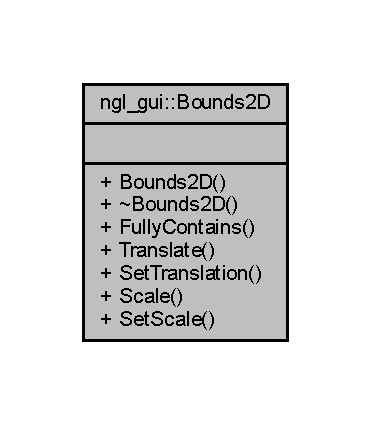
\includegraphics[width=178pt]{classngl__gui_1_1_bounds2_d__coll__graph}
\end{center}
\end{figure}
\subsection*{Public Member Functions}
\begin{DoxyCompactItemize}
\item 
\mbox{\hyperlink{classngl__gui_1_1_bounds2_d_a4e70541988d6a2125c03ac2f5f8700a3}{Bounds2D}} ()
\item 
virtual \mbox{\hyperlink{classngl__gui_1_1_bounds2_d_a660706507adf515494e5d90572f4d2ec}{$\sim$\+Bounds2D}} ()
\item 
bool \mbox{\hyperlink{classngl__gui_1_1_bounds2_d_a79aa9cec12a3492a892b6384581c11b7}{Fully\+Contains}} (const \mbox{\hyperlink{classngl__gui_1_1_bounds2_d}{Bounds2D}} \&bounds)
\item 
void \mbox{\hyperlink{classngl__gui_1_1_bounds2_d_ae194f1a4c97b962c45354af32b54e439}{Translate}} (const glm\+::vec2 \&val)
\item 
void \mbox{\hyperlink{classngl__gui_1_1_bounds2_d_ad0aa8c5230b5986564f1bfdec2c19883}{Set\+Translation}} (const glm\+::vec2 \&val)
\item 
void \mbox{\hyperlink{classngl__gui_1_1_bounds2_d_a1fbdca184f173b6b274069df064b0dee}{Scale}} (const glm\+::vec2 \&val)
\item 
void \mbox{\hyperlink{classngl__gui_1_1_bounds2_d_a79ecc23f1d8fa2bc72b02c94ec562bc3}{Set\+Scale}} (const glm\+::vec2 \&val)
\end{DoxyCompactItemize}


\subsection{Constructor \& Destructor Documentation}
\mbox{\Hypertarget{classngl__gui_1_1_bounds2_d_a4e70541988d6a2125c03ac2f5f8700a3}\label{classngl__gui_1_1_bounds2_d_a4e70541988d6a2125c03ac2f5f8700a3}} 
\index{ngl\+\_\+gui\+::\+Bounds2D@{ngl\+\_\+gui\+::\+Bounds2D}!Bounds2D@{Bounds2D}}
\index{Bounds2D@{Bounds2D}!ngl\+\_\+gui\+::\+Bounds2D@{ngl\+\_\+gui\+::\+Bounds2D}}
\subsubsection{\texorpdfstring{Bounds2\+D()}{Bounds2D()}}
{\footnotesize\ttfamily ngl\+\_\+gui\+::\+Bounds2\+D\+::\+Bounds2D (\begin{DoxyParamCaption}{ }\end{DoxyParamCaption})\hspace{0.3cm}{\ttfamily [explicit]}}

\mbox{\Hypertarget{classngl__gui_1_1_bounds2_d_a660706507adf515494e5d90572f4d2ec}\label{classngl__gui_1_1_bounds2_d_a660706507adf515494e5d90572f4d2ec}} 
\index{ngl\+\_\+gui\+::\+Bounds2D@{ngl\+\_\+gui\+::\+Bounds2D}!````~Bounds2D@{$\sim$\+Bounds2D}}
\index{````~Bounds2D@{$\sim$\+Bounds2D}!ngl\+\_\+gui\+::\+Bounds2D@{ngl\+\_\+gui\+::\+Bounds2D}}
\subsubsection{\texorpdfstring{$\sim$\+Bounds2\+D()}{~Bounds2D()}}
{\footnotesize\ttfamily ngl\+\_\+gui\+::\+Bounds2\+D\+::$\sim$\+Bounds2D (\begin{DoxyParamCaption}{ }\end{DoxyParamCaption})\hspace{0.3cm}{\ttfamily [virtual]}}



\subsection{Member Function Documentation}
\mbox{\Hypertarget{classngl__gui_1_1_bounds2_d_a79aa9cec12a3492a892b6384581c11b7}\label{classngl__gui_1_1_bounds2_d_a79aa9cec12a3492a892b6384581c11b7}} 
\index{ngl\+\_\+gui\+::\+Bounds2D@{ngl\+\_\+gui\+::\+Bounds2D}!Fully\+Contains@{Fully\+Contains}}
\index{Fully\+Contains@{Fully\+Contains}!ngl\+\_\+gui\+::\+Bounds2D@{ngl\+\_\+gui\+::\+Bounds2D}}
\subsubsection{\texorpdfstring{Fully\+Contains()}{FullyContains()}}
{\footnotesize\ttfamily bool ngl\+\_\+gui\+::\+Bounds2\+D\+::\+Fully\+Contains (\begin{DoxyParamCaption}\item[{const \mbox{\hyperlink{classngl__gui_1_1_bounds2_d}{Bounds2D}} \&}]{bounds }\end{DoxyParamCaption})}

\mbox{\Hypertarget{classngl__gui_1_1_bounds2_d_a1fbdca184f173b6b274069df064b0dee}\label{classngl__gui_1_1_bounds2_d_a1fbdca184f173b6b274069df064b0dee}} 
\index{ngl\+\_\+gui\+::\+Bounds2D@{ngl\+\_\+gui\+::\+Bounds2D}!Scale@{Scale}}
\index{Scale@{Scale}!ngl\+\_\+gui\+::\+Bounds2D@{ngl\+\_\+gui\+::\+Bounds2D}}
\subsubsection{\texorpdfstring{Scale()}{Scale()}}
{\footnotesize\ttfamily void ngl\+\_\+gui\+::\+Bounds2\+D\+::\+Scale (\begin{DoxyParamCaption}\item[{const glm\+::vec2 \&}]{val }\end{DoxyParamCaption})}

\mbox{\Hypertarget{classngl__gui_1_1_bounds2_d_a79ecc23f1d8fa2bc72b02c94ec562bc3}\label{classngl__gui_1_1_bounds2_d_a79ecc23f1d8fa2bc72b02c94ec562bc3}} 
\index{ngl\+\_\+gui\+::\+Bounds2D@{ngl\+\_\+gui\+::\+Bounds2D}!Set\+Scale@{Set\+Scale}}
\index{Set\+Scale@{Set\+Scale}!ngl\+\_\+gui\+::\+Bounds2D@{ngl\+\_\+gui\+::\+Bounds2D}}
\subsubsection{\texorpdfstring{Set\+Scale()}{SetScale()}}
{\footnotesize\ttfamily void ngl\+\_\+gui\+::\+Bounds2\+D\+::\+Set\+Scale (\begin{DoxyParamCaption}\item[{const glm\+::vec2 \&}]{val }\end{DoxyParamCaption})}

\mbox{\Hypertarget{classngl__gui_1_1_bounds2_d_ad0aa8c5230b5986564f1bfdec2c19883}\label{classngl__gui_1_1_bounds2_d_ad0aa8c5230b5986564f1bfdec2c19883}} 
\index{ngl\+\_\+gui\+::\+Bounds2D@{ngl\+\_\+gui\+::\+Bounds2D}!Set\+Translation@{Set\+Translation}}
\index{Set\+Translation@{Set\+Translation}!ngl\+\_\+gui\+::\+Bounds2D@{ngl\+\_\+gui\+::\+Bounds2D}}
\subsubsection{\texorpdfstring{Set\+Translation()}{SetTranslation()}}
{\footnotesize\ttfamily void ngl\+\_\+gui\+::\+Bounds2\+D\+::\+Set\+Translation (\begin{DoxyParamCaption}\item[{const glm\+::vec2 \&}]{val }\end{DoxyParamCaption})}

\mbox{\Hypertarget{classngl__gui_1_1_bounds2_d_ae194f1a4c97b962c45354af32b54e439}\label{classngl__gui_1_1_bounds2_d_ae194f1a4c97b962c45354af32b54e439}} 
\index{ngl\+\_\+gui\+::\+Bounds2D@{ngl\+\_\+gui\+::\+Bounds2D}!Translate@{Translate}}
\index{Translate@{Translate}!ngl\+\_\+gui\+::\+Bounds2D@{ngl\+\_\+gui\+::\+Bounds2D}}
\subsubsection{\texorpdfstring{Translate()}{Translate()}}
{\footnotesize\ttfamily void ngl\+\_\+gui\+::\+Bounds2\+D\+::\+Translate (\begin{DoxyParamCaption}\item[{const glm\+::vec2 \&}]{val }\end{DoxyParamCaption})}



The documentation for this class was generated from the following files\+:\begin{DoxyCompactItemize}
\item 
D\+:/\+Library/\+Documents/\+Job/\+Forschungsmaster/\+Projekte/\+Eye\+Candy3\+D/\+Eye\+Candy3\+D/include/\+E\+C3\+D/\+G\+U\+I/\mbox{\hyperlink{_bounds2_d_8h}{Bounds2\+D.\+h}}\item 
D\+:/\+Library/\+Documents/\+Job/\+Forschungsmaster/\+Projekte/\+Eye\+Candy3\+D/\+Eye\+Candy3\+D/src/\+G\+U\+I/\mbox{\hyperlink{_bounds2_d_8cpp}{Bounds2\+D.\+cpp}}\end{DoxyCompactItemize}

\hypertarget{classngl__gui_1_1_button}{}\section{ngl\+\_\+gui\+:\+:Button Class Reference}
\label{classngl__gui_1_1_button}\index{ngl\+\_\+gui\+::\+Button@{ngl\+\_\+gui\+::\+Button}}


{\ttfamily \#include $<$Button.\+h$>$}



Inheritance diagram for ngl\+\_\+gui\+:\+:Button\+:\nopagebreak
\begin{figure}[H]
\begin{center}
\leavevmode
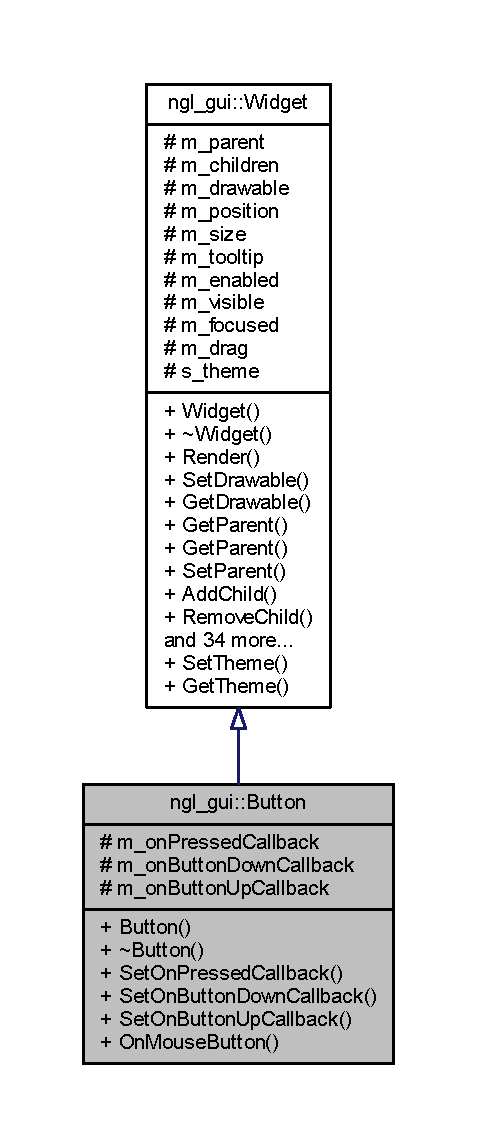
\includegraphics[height=550pt]{classngl__gui_1_1_button__inherit__graph}
\end{center}
\end{figure}


Collaboration diagram for ngl\+\_\+gui\+:\+:Button\+:
\nopagebreak
\begin{figure}[H]
\begin{center}
\leavevmode
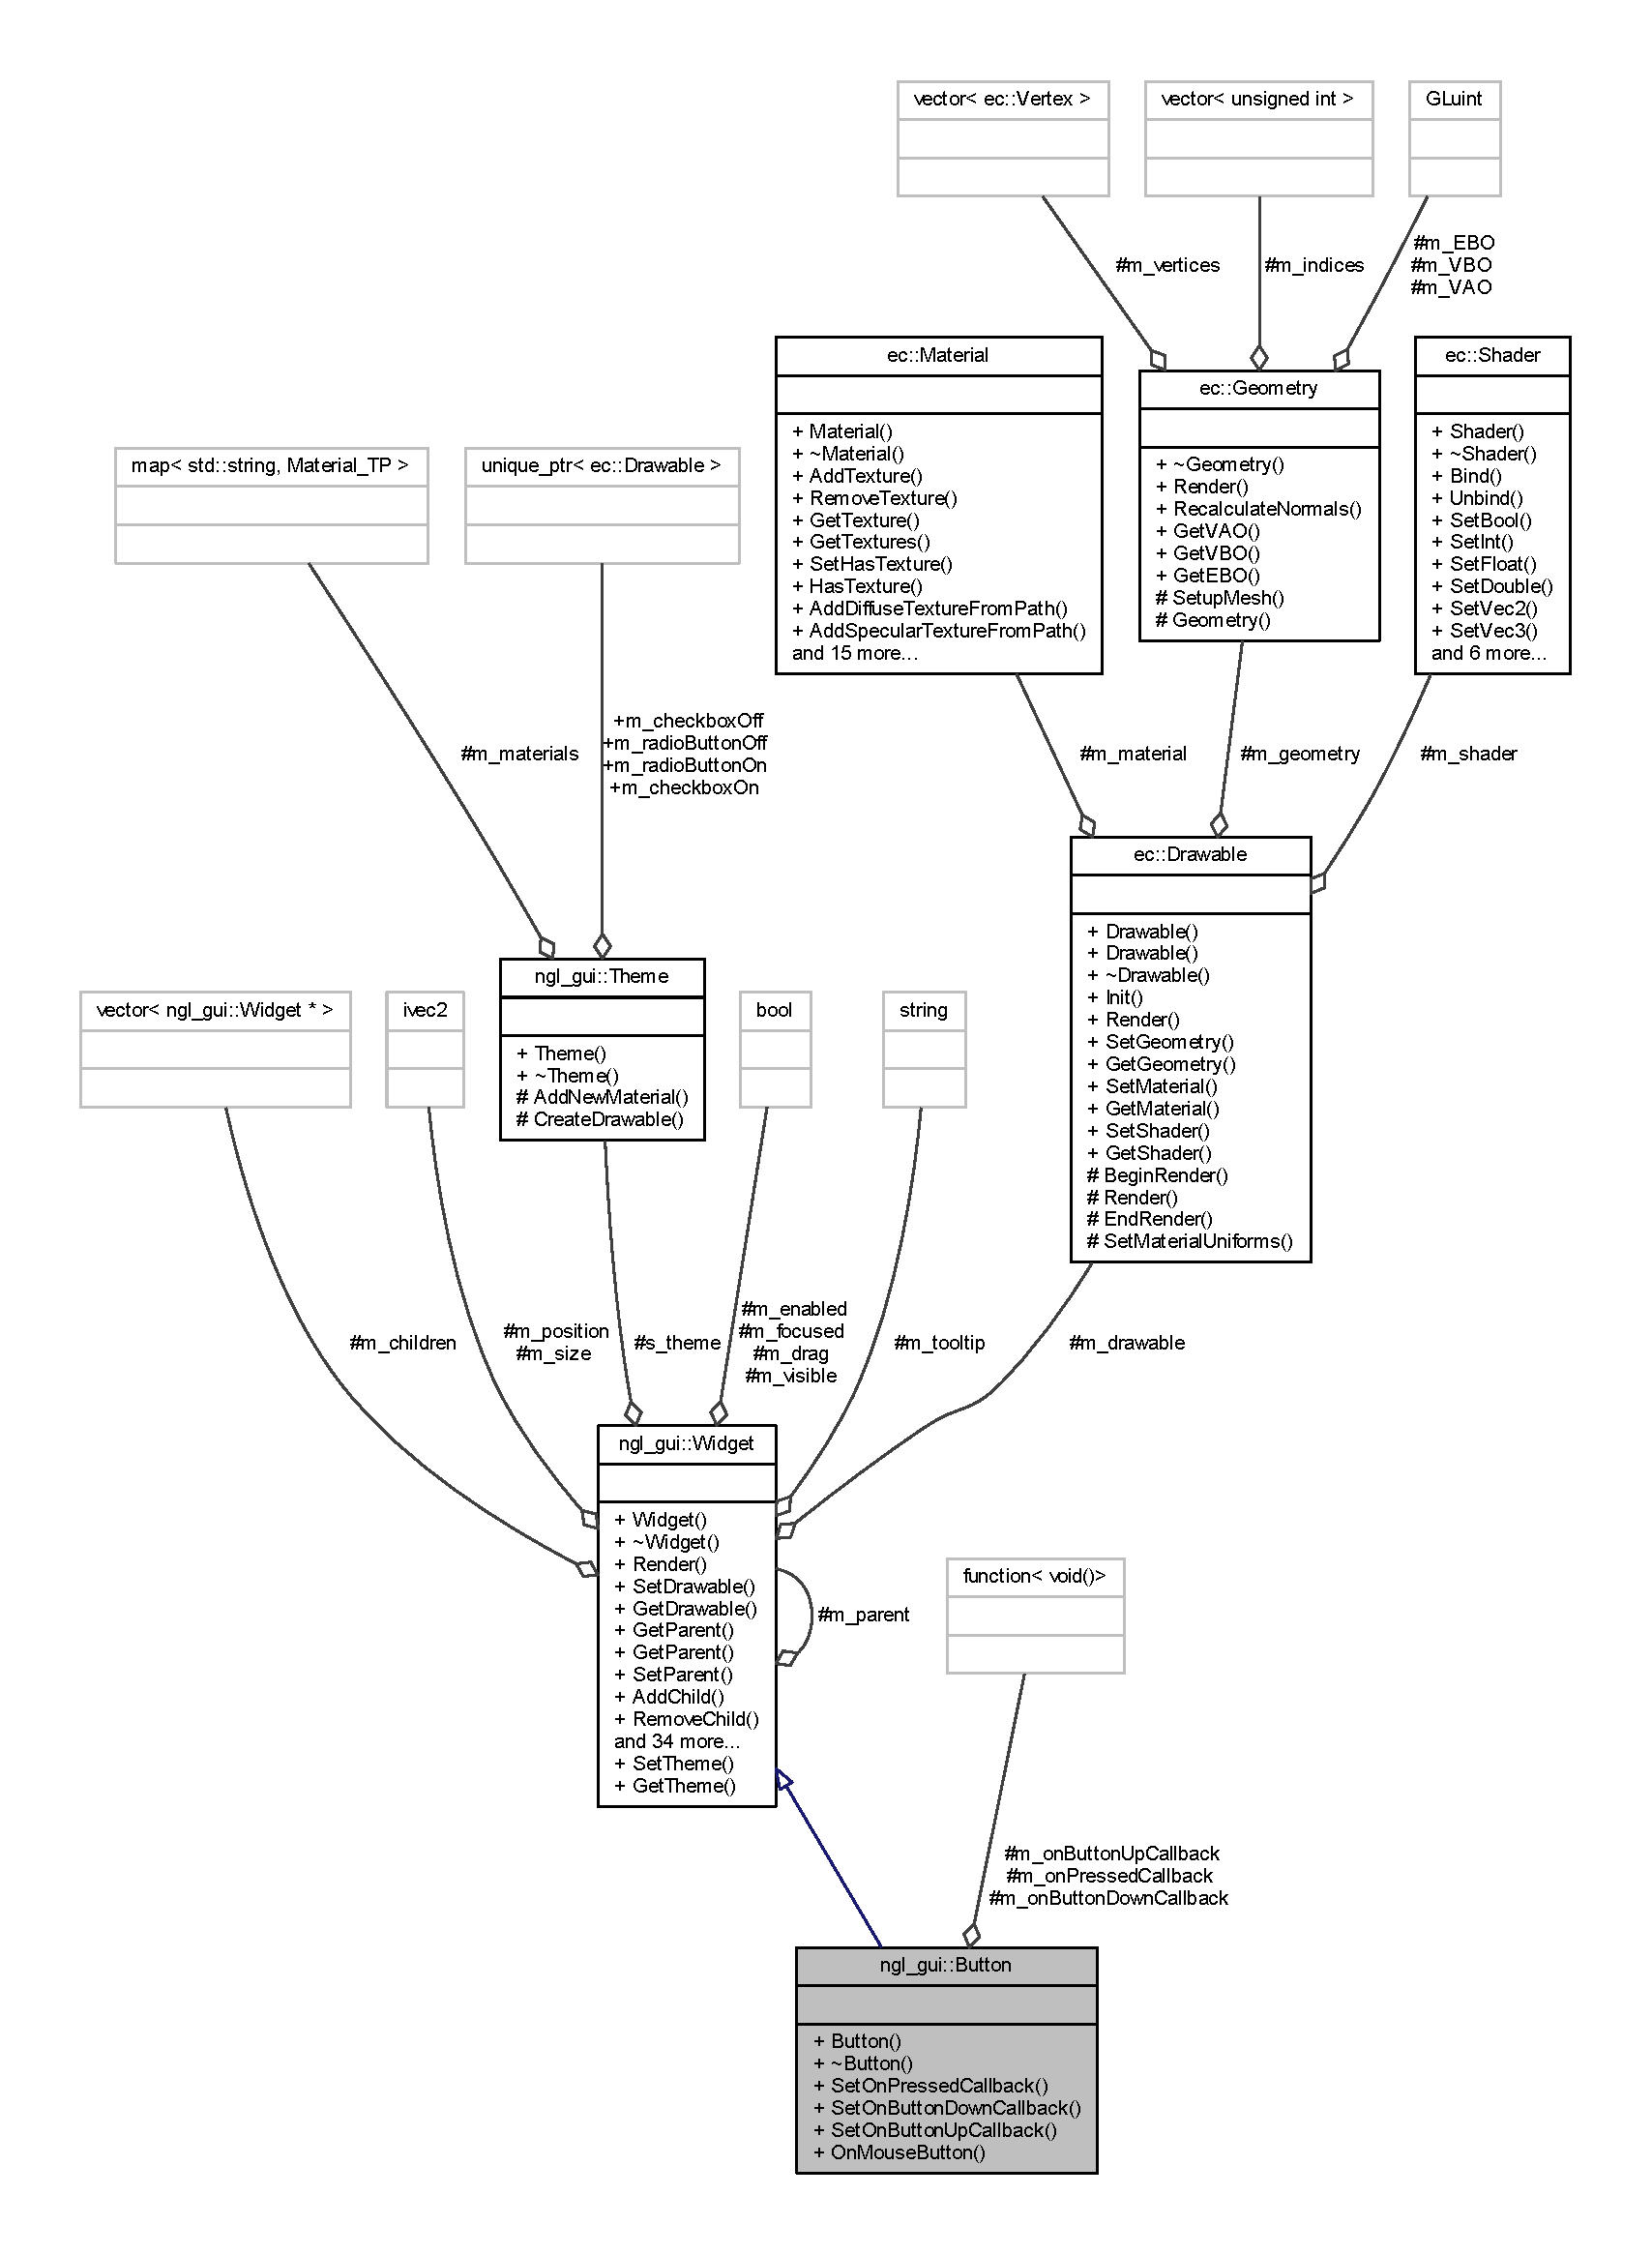
\includegraphics[width=350pt]{classngl__gui_1_1_button__coll__graph}
\end{center}
\end{figure}
\subsection*{Public Member Functions}
\begin{DoxyCompactItemize}
\item 
\mbox{\hyperlink{classngl__gui_1_1_button_ac153b6ad7d4656c9a66699fe91fb0529}{Button}} (\mbox{\hyperlink{classngl__gui_1_1_widget}{Widget}} $\ast$parent)
\item 
virtual \mbox{\hyperlink{classngl__gui_1_1_button_ae33e1e09f1f50ddc5f5820dbc90ff43f}{$\sim$\+Button}} ()
\item 
void \mbox{\hyperlink{classngl__gui_1_1_button_a604ffbd593690a3f4e044b357f678fdb}{Set\+On\+Pressed\+Callback}} (std\+::function$<$ void()$>$ callback)
\item 
void \mbox{\hyperlink{classngl__gui_1_1_button_a739337d2d66c43de5c0c6a7d0bc3552b}{Set\+On\+Button\+Down\+Callback}} (std\+::function$<$ void()$>$ callback)
\item 
void \mbox{\hyperlink{classngl__gui_1_1_button_ab1b47991bb39a0d905235fb185c3dd0a}{Set\+On\+Button\+Up\+Callback}} (std\+::function$<$ void()$>$ callback)
\item 
virtual bool \mbox{\hyperlink{classngl__gui_1_1_button_a1022c031cb9bb6658d8a6bb22295508d}{On\+Mouse\+Button}} (const glm\+::ivec2 \&position, int button, int mods, bool pressed) override
\end{DoxyCompactItemize}
\subsection*{Protected Attributes}
\begin{DoxyCompactItemize}
\item 
std\+::function$<$ void()$>$ \mbox{\hyperlink{classngl__gui_1_1_button_af090b33093b5b400f3f28e22f82d7fd2}{m\+\_\+on\+Pressed\+Callback}}
\item 
std\+::function$<$ void()$>$ \mbox{\hyperlink{classngl__gui_1_1_button_a87f1bdc19a384c649c0e299e8d0842a4}{m\+\_\+on\+Button\+Down\+Callback}}
\item 
std\+::function$<$ void()$>$ \mbox{\hyperlink{classngl__gui_1_1_button_a12f95fd476017194b064040fe071f4f7}{m\+\_\+on\+Button\+Up\+Callback}}
\end{DoxyCompactItemize}
\subsection*{Additional Inherited Members}


\subsection{Constructor \& Destructor Documentation}
\mbox{\Hypertarget{classngl__gui_1_1_button_ac153b6ad7d4656c9a66699fe91fb0529}\label{classngl__gui_1_1_button_ac153b6ad7d4656c9a66699fe91fb0529}} 
\index{ngl\+\_\+gui\+::\+Button@{ngl\+\_\+gui\+::\+Button}!Button@{Button}}
\index{Button@{Button}!ngl\+\_\+gui\+::\+Button@{ngl\+\_\+gui\+::\+Button}}
\subsubsection{\texorpdfstring{Button()}{Button()}}
{\footnotesize\ttfamily ngl\+\_\+gui\+::\+Button\+::\+Button (\begin{DoxyParamCaption}\item[{\mbox{\hyperlink{classngl__gui_1_1_widget}{Widget}} $\ast$}]{parent }\end{DoxyParamCaption})\hspace{0.3cm}{\ttfamily [explicit]}}

\mbox{\Hypertarget{classngl__gui_1_1_button_ae33e1e09f1f50ddc5f5820dbc90ff43f}\label{classngl__gui_1_1_button_ae33e1e09f1f50ddc5f5820dbc90ff43f}} 
\index{ngl\+\_\+gui\+::\+Button@{ngl\+\_\+gui\+::\+Button}!````~Button@{$\sim$\+Button}}
\index{````~Button@{$\sim$\+Button}!ngl\+\_\+gui\+::\+Button@{ngl\+\_\+gui\+::\+Button}}
\subsubsection{\texorpdfstring{$\sim$\+Button()}{~Button()}}
{\footnotesize\ttfamily ngl\+\_\+gui\+::\+Button\+::$\sim$\+Button (\begin{DoxyParamCaption}{ }\end{DoxyParamCaption})\hspace{0.3cm}{\ttfamily [virtual]}}



\subsection{Member Function Documentation}
\mbox{\Hypertarget{classngl__gui_1_1_button_a1022c031cb9bb6658d8a6bb22295508d}\label{classngl__gui_1_1_button_a1022c031cb9bb6658d8a6bb22295508d}} 
\index{ngl\+\_\+gui\+::\+Button@{ngl\+\_\+gui\+::\+Button}!On\+Mouse\+Button@{On\+Mouse\+Button}}
\index{On\+Mouse\+Button@{On\+Mouse\+Button}!ngl\+\_\+gui\+::\+Button@{ngl\+\_\+gui\+::\+Button}}
\subsubsection{\texorpdfstring{On\+Mouse\+Button()}{OnMouseButton()}}
{\footnotesize\ttfamily bool ngl\+\_\+gui\+::\+Button\+::\+On\+Mouse\+Button (\begin{DoxyParamCaption}\item[{const glm\+::ivec2 \&}]{position,  }\item[{int}]{button,  }\item[{int}]{mods,  }\item[{bool}]{pressed }\end{DoxyParamCaption})\hspace{0.3cm}{\ttfamily [override]}, {\ttfamily [virtual]}}



Reimplemented from \mbox{\hyperlink{classngl__gui_1_1_widget_a721b18dc7a09b0b7b4ff0c02162409b8}{ngl\+\_\+gui\+::\+Widget}}.

\mbox{\Hypertarget{classngl__gui_1_1_button_a739337d2d66c43de5c0c6a7d0bc3552b}\label{classngl__gui_1_1_button_a739337d2d66c43de5c0c6a7d0bc3552b}} 
\index{ngl\+\_\+gui\+::\+Button@{ngl\+\_\+gui\+::\+Button}!Set\+On\+Button\+Down\+Callback@{Set\+On\+Button\+Down\+Callback}}
\index{Set\+On\+Button\+Down\+Callback@{Set\+On\+Button\+Down\+Callback}!ngl\+\_\+gui\+::\+Button@{ngl\+\_\+gui\+::\+Button}}
\subsubsection{\texorpdfstring{Set\+On\+Button\+Down\+Callback()}{SetOnButtonDownCallback()}}
{\footnotesize\ttfamily void ngl\+\_\+gui\+::\+Button\+::\+Set\+On\+Button\+Down\+Callback (\begin{DoxyParamCaption}\item[{std\+::function$<$ void()$>$}]{callback }\end{DoxyParamCaption})}

\mbox{\Hypertarget{classngl__gui_1_1_button_ab1b47991bb39a0d905235fb185c3dd0a}\label{classngl__gui_1_1_button_ab1b47991bb39a0d905235fb185c3dd0a}} 
\index{ngl\+\_\+gui\+::\+Button@{ngl\+\_\+gui\+::\+Button}!Set\+On\+Button\+Up\+Callback@{Set\+On\+Button\+Up\+Callback}}
\index{Set\+On\+Button\+Up\+Callback@{Set\+On\+Button\+Up\+Callback}!ngl\+\_\+gui\+::\+Button@{ngl\+\_\+gui\+::\+Button}}
\subsubsection{\texorpdfstring{Set\+On\+Button\+Up\+Callback()}{SetOnButtonUpCallback()}}
{\footnotesize\ttfamily void ngl\+\_\+gui\+::\+Button\+::\+Set\+On\+Button\+Up\+Callback (\begin{DoxyParamCaption}\item[{std\+::function$<$ void()$>$}]{callback }\end{DoxyParamCaption})}

\mbox{\Hypertarget{classngl__gui_1_1_button_a604ffbd593690a3f4e044b357f678fdb}\label{classngl__gui_1_1_button_a604ffbd593690a3f4e044b357f678fdb}} 
\index{ngl\+\_\+gui\+::\+Button@{ngl\+\_\+gui\+::\+Button}!Set\+On\+Pressed\+Callback@{Set\+On\+Pressed\+Callback}}
\index{Set\+On\+Pressed\+Callback@{Set\+On\+Pressed\+Callback}!ngl\+\_\+gui\+::\+Button@{ngl\+\_\+gui\+::\+Button}}
\subsubsection{\texorpdfstring{Set\+On\+Pressed\+Callback()}{SetOnPressedCallback()}}
{\footnotesize\ttfamily void ngl\+\_\+gui\+::\+Button\+::\+Set\+On\+Pressed\+Callback (\begin{DoxyParamCaption}\item[{std\+::function$<$ void()$>$}]{callback }\end{DoxyParamCaption})}



\subsection{Member Data Documentation}
\mbox{\Hypertarget{classngl__gui_1_1_button_a87f1bdc19a384c649c0e299e8d0842a4}\label{classngl__gui_1_1_button_a87f1bdc19a384c649c0e299e8d0842a4}} 
\index{ngl\+\_\+gui\+::\+Button@{ngl\+\_\+gui\+::\+Button}!m\+\_\+on\+Button\+Down\+Callback@{m\+\_\+on\+Button\+Down\+Callback}}
\index{m\+\_\+on\+Button\+Down\+Callback@{m\+\_\+on\+Button\+Down\+Callback}!ngl\+\_\+gui\+::\+Button@{ngl\+\_\+gui\+::\+Button}}
\subsubsection{\texorpdfstring{m\+\_\+on\+Button\+Down\+Callback}{m\_onButtonDownCallback}}
{\footnotesize\ttfamily std\+::function$<$void()$>$ ngl\+\_\+gui\+::\+Button\+::m\+\_\+on\+Button\+Down\+Callback\hspace{0.3cm}{\ttfamily [protected]}}

\mbox{\Hypertarget{classngl__gui_1_1_button_a12f95fd476017194b064040fe071f4f7}\label{classngl__gui_1_1_button_a12f95fd476017194b064040fe071f4f7}} 
\index{ngl\+\_\+gui\+::\+Button@{ngl\+\_\+gui\+::\+Button}!m\+\_\+on\+Button\+Up\+Callback@{m\+\_\+on\+Button\+Up\+Callback}}
\index{m\+\_\+on\+Button\+Up\+Callback@{m\+\_\+on\+Button\+Up\+Callback}!ngl\+\_\+gui\+::\+Button@{ngl\+\_\+gui\+::\+Button}}
\subsubsection{\texorpdfstring{m\+\_\+on\+Button\+Up\+Callback}{m\_onButtonUpCallback}}
{\footnotesize\ttfamily std\+::function$<$void()$>$ ngl\+\_\+gui\+::\+Button\+::m\+\_\+on\+Button\+Up\+Callback\hspace{0.3cm}{\ttfamily [protected]}}

\mbox{\Hypertarget{classngl__gui_1_1_button_af090b33093b5b400f3f28e22f82d7fd2}\label{classngl__gui_1_1_button_af090b33093b5b400f3f28e22f82d7fd2}} 
\index{ngl\+\_\+gui\+::\+Button@{ngl\+\_\+gui\+::\+Button}!m\+\_\+on\+Pressed\+Callback@{m\+\_\+on\+Pressed\+Callback}}
\index{m\+\_\+on\+Pressed\+Callback@{m\+\_\+on\+Pressed\+Callback}!ngl\+\_\+gui\+::\+Button@{ngl\+\_\+gui\+::\+Button}}
\subsubsection{\texorpdfstring{m\+\_\+on\+Pressed\+Callback}{m\_onPressedCallback}}
{\footnotesize\ttfamily std\+::function$<$void()$>$ ngl\+\_\+gui\+::\+Button\+::m\+\_\+on\+Pressed\+Callback\hspace{0.3cm}{\ttfamily [protected]}}



The documentation for this class was generated from the following files\+:\begin{DoxyCompactItemize}
\item 
D\+:/\+Library/\+Documents/\+Job/\+Forschungsmaster/\+Projekte/\+Eye\+Candy3\+D/\+Eye\+Candy3\+D/include/\+E\+C3\+D/\+G\+U\+I/\mbox{\hyperlink{_button_8h}{Button.\+h}}\item 
D\+:/\+Library/\+Documents/\+Job/\+Forschungsmaster/\+Projekte/\+Eye\+Candy3\+D/\+Eye\+Candy3\+D/src/\+G\+U\+I/\mbox{\hyperlink{_button_8cpp}{Button.\+cpp}}\end{DoxyCompactItemize}

\hypertarget{classec_1_1_camera}{}\section{ec\+:\+:Camera Class Reference}
\label{classec_1_1_camera}\index{ec\+::\+Camera@{ec\+::\+Camera}}


{\ttfamily \#include $<$Camera.\+h$>$}



Inheritance diagram for ec\+:\+:Camera\+:
\nopagebreak
\begin{figure}[H]
\begin{center}
\leavevmode
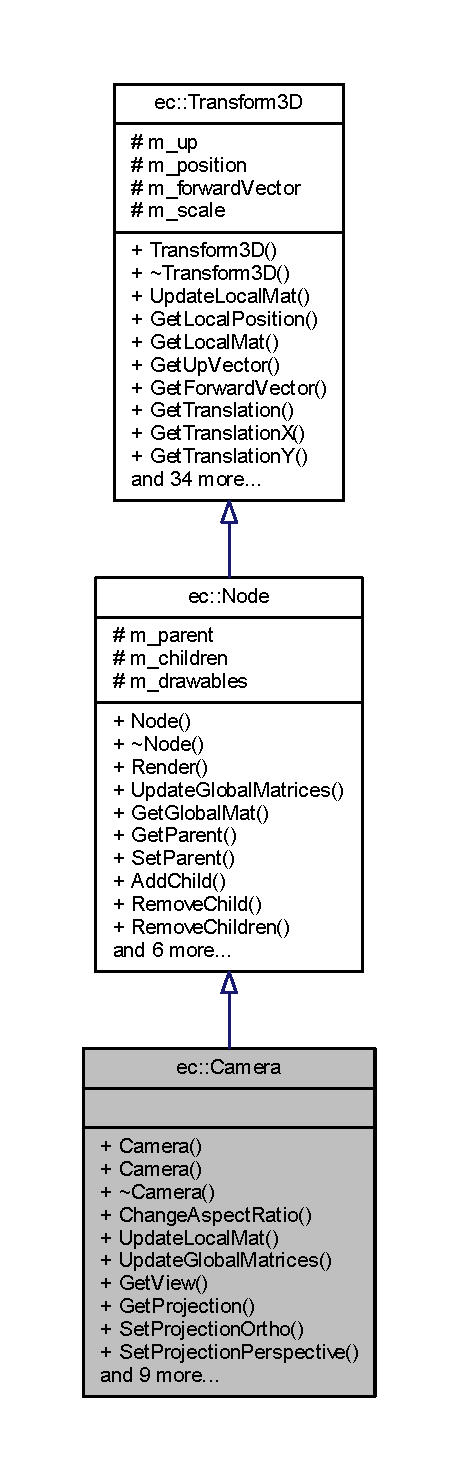
\includegraphics[height=550pt]{classec_1_1_camera__inherit__graph}
\end{center}
\end{figure}


Collaboration diagram for ec\+:\+:Camera\+:
\nopagebreak
\begin{figure}[H]
\begin{center}
\leavevmode
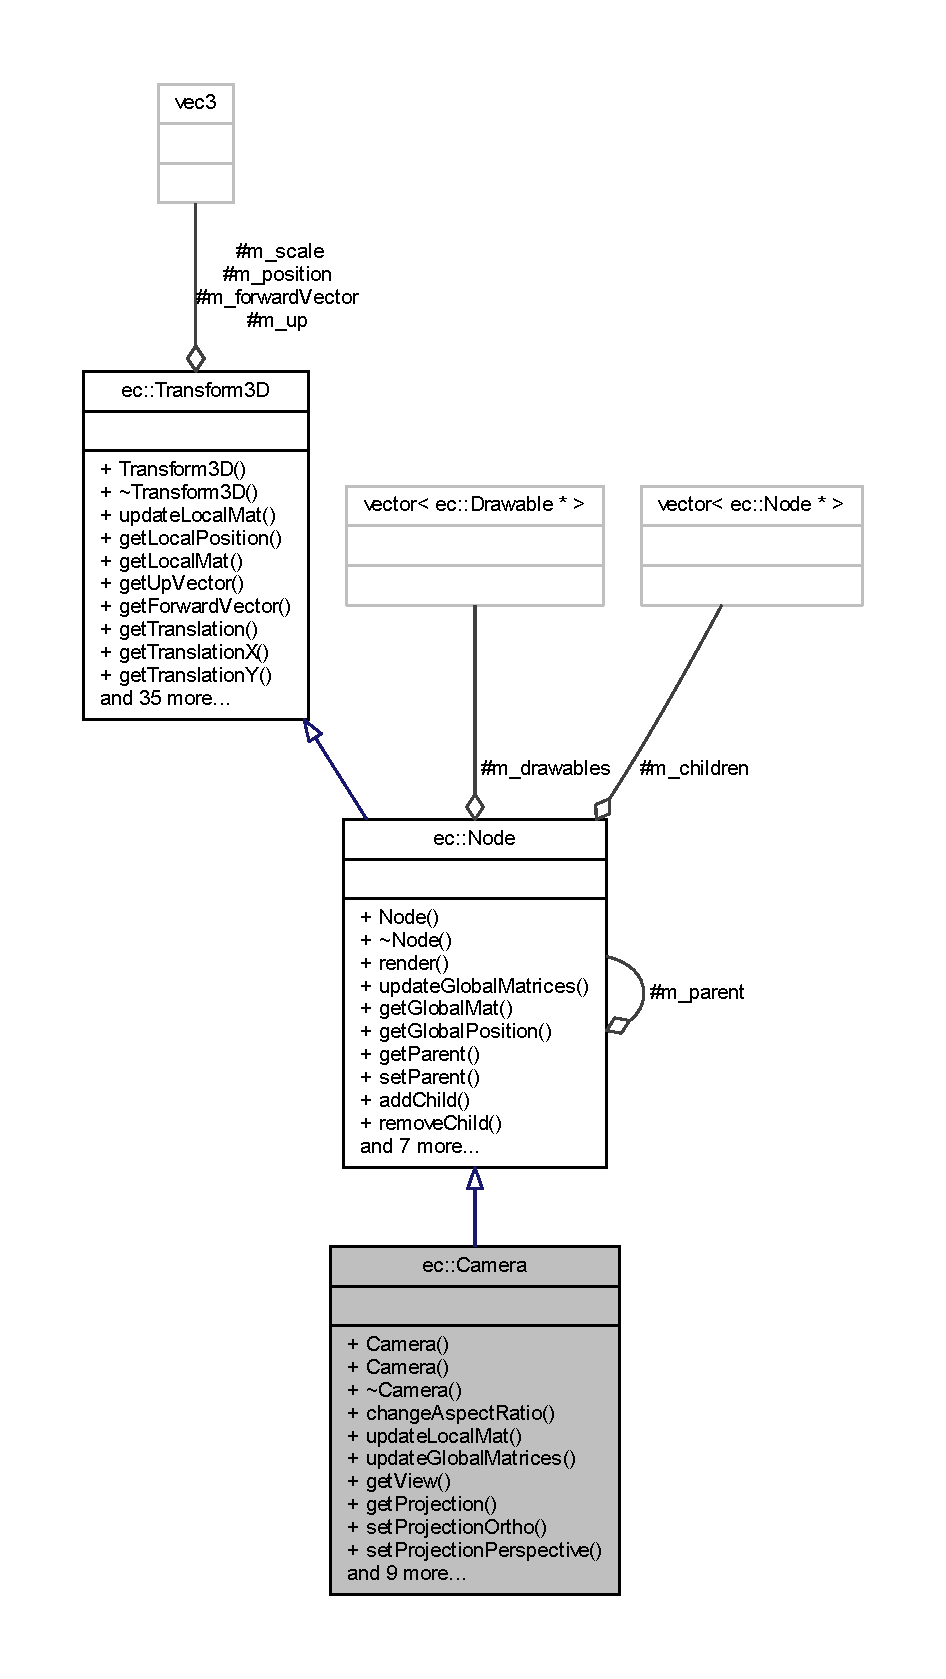
\includegraphics[height=550pt]{classec_1_1_camera__coll__graph}
\end{center}
\end{figure}
\subsection*{Public Member Functions}
\begin{DoxyCompactItemize}
\item 
\mbox{\hyperlink{classec_1_1_camera_a5b8034c32e082171bdb61033781cdcc3}{Camera}} (\mbox{\hyperlink{classec_1_1_scene}{Scene}} $\ast$scene)
\item 
\mbox{\hyperlink{classec_1_1_camera_ab5fa55c91ae586754b613c3e8f33b31c}{Camera}} (\mbox{\hyperlink{classec_1_1_scene}{Scene}} $\ast$scene, const \mbox{\hyperlink{classec_1_1_viewport}{Viewport}} \&viewport)
\item 
\mbox{\hyperlink{classec_1_1_camera_a11d706554e37d6dde0b9313a445cbd4b}{$\sim$\+Camera}} ()
\item 
void \mbox{\hyperlink{classec_1_1_camera_ad3790ce4b558aa906fe00e25d8c8c1ed}{Change\+Aspect\+Ratio}} (float aspect)
\item 
virtual void \mbox{\hyperlink{classec_1_1_camera_ab9b2d59d1755a56d67c13a5539b7e033}{Update\+Local\+Mat}} () override
\item 
virtual void \mbox{\hyperlink{classec_1_1_camera_abbdd88f9b352d34fef473064e2ccd625}{Update\+Global\+Matrices}} (const glm\+::mat4 \&m\+\_\+parent\+Mat) override
\item 
const glm\+::mat4 \& \mbox{\hyperlink{classec_1_1_camera_ad5ed2007c501081561fd8ee894f86ae0}{Get\+View}} () const
\item 
const glm\+::mat4 \& \mbox{\hyperlink{classec_1_1_camera_a9c52ad9d4077faf50d1d7170d08e1f13}{Get\+Projection}} () const
\item 
void \mbox{\hyperlink{classec_1_1_camera_ad17ef414e3a08344607a4929f89c7ab3}{Set\+Projection\+Ortho}} ()
\item 
void \mbox{\hyperlink{classec_1_1_camera_a5d6b64ba57b209cca822f4ca9e278a44}{Set\+Projection\+Perspective}} ()
\item 
void \mbox{\hyperlink{classec_1_1_camera_a9af6e8b9a37d5494b5ddf6f098f463bc}{Set\+F\+OV}} (const float fov)
\item 
float \mbox{\hyperlink{classec_1_1_camera_a076c35547c2e64166ac3307b13292131}{Get\+F\+OV}} () const
\item 
void \mbox{\hyperlink{classec_1_1_camera_af2069e18dee1923fb5d9c77bf9366479}{Set\+Near}} (const float near)
\item 
float \mbox{\hyperlink{classec_1_1_camera_abf0024083abfe06c0e5de606ee2b8912}{Get\+Near}} () const
\item 
void \mbox{\hyperlink{classec_1_1_camera_adb376b3c35aed1e7681f74ddbbe9fa25}{Set\+Far}} (const float far)
\item 
float \mbox{\hyperlink{classec_1_1_camera_a5bdbf9c5001e666bed13a5c75fd1c88f}{Get\+Far}} () const
\item 
\mbox{\hyperlink{classec_1_1_scene}{Scene}} $\ast$ \mbox{\hyperlink{classec_1_1_camera_a77f8c613ff916b697bdab94d4a610e5d}{Get\+Scene}} () const
\item 
const \mbox{\hyperlink{classec_1_1_viewport}{Viewport}} \& \mbox{\hyperlink{classec_1_1_camera_a6997f9c09e6cf43b1e7440eb2af83eb2}{Get\+Viewport}} () const
\item 
void \mbox{\hyperlink{classec_1_1_camera_a30dab960758a3614624cada979abdd5a}{Set\+Viewport}} (const \mbox{\hyperlink{classec_1_1_viewport}{Viewport}} \&viewport)
\end{DoxyCompactItemize}
\subsection*{Additional Inherited Members}


\subsection{Detailed Description}
A camera encapsulates a view and a projection matrix. It is used to render the related scene. It contains a viewport, which defines the area of the render target the scene should be rendered into. 

\subsection{Constructor \& Destructor Documentation}
\mbox{\Hypertarget{classec_1_1_camera_a5b8034c32e082171bdb61033781cdcc3}\label{classec_1_1_camera_a5b8034c32e082171bdb61033781cdcc3}} 
\index{ec\+::\+Camera@{ec\+::\+Camera}!Camera@{Camera}}
\index{Camera@{Camera}!ec\+::\+Camera@{ec\+::\+Camera}}
\subsubsection{\texorpdfstring{Camera()}{Camera()}\hspace{0.1cm}{\footnotesize\ttfamily [1/2]}}
{\footnotesize\ttfamily ec\+::\+Camera\+::\+Camera (\begin{DoxyParamCaption}\item[{\mbox{\hyperlink{classec_1_1_scene}{Scene}} $\ast$}]{scene }\end{DoxyParamCaption})\hspace{0.3cm}{\ttfamily [explicit]}}

\mbox{\Hypertarget{classec_1_1_camera_ab5fa55c91ae586754b613c3e8f33b31c}\label{classec_1_1_camera_ab5fa55c91ae586754b613c3e8f33b31c}} 
\index{ec\+::\+Camera@{ec\+::\+Camera}!Camera@{Camera}}
\index{Camera@{Camera}!ec\+::\+Camera@{ec\+::\+Camera}}
\subsubsection{\texorpdfstring{Camera()}{Camera()}\hspace{0.1cm}{\footnotesize\ttfamily [2/2]}}
{\footnotesize\ttfamily ec\+::\+Camera\+::\+Camera (\begin{DoxyParamCaption}\item[{\mbox{\hyperlink{classec_1_1_scene}{Scene}} $\ast$}]{scene,  }\item[{const \mbox{\hyperlink{classec_1_1_viewport}{Viewport}} \&}]{viewport }\end{DoxyParamCaption})\hspace{0.3cm}{\ttfamily [explicit]}}

\mbox{\Hypertarget{classec_1_1_camera_a11d706554e37d6dde0b9313a445cbd4b}\label{classec_1_1_camera_a11d706554e37d6dde0b9313a445cbd4b}} 
\index{ec\+::\+Camera@{ec\+::\+Camera}!````~Camera@{$\sim$\+Camera}}
\index{````~Camera@{$\sim$\+Camera}!ec\+::\+Camera@{ec\+::\+Camera}}
\subsubsection{\texorpdfstring{$\sim$\+Camera()}{~Camera()}}
{\footnotesize\ttfamily ec\+::\+Camera\+::$\sim$\+Camera (\begin{DoxyParamCaption}{ }\end{DoxyParamCaption})}



\subsection{Member Function Documentation}
\mbox{\Hypertarget{classec_1_1_camera_ad3790ce4b558aa906fe00e25d8c8c1ed}\label{classec_1_1_camera_ad3790ce4b558aa906fe00e25d8c8c1ed}} 
\index{ec\+::\+Camera@{ec\+::\+Camera}!Change\+Aspect\+Ratio@{Change\+Aspect\+Ratio}}
\index{Change\+Aspect\+Ratio@{Change\+Aspect\+Ratio}!ec\+::\+Camera@{ec\+::\+Camera}}
\subsubsection{\texorpdfstring{Change\+Aspect\+Ratio()}{ChangeAspectRatio()}}
{\footnotesize\ttfamily void ec\+::\+Camera\+::\+Change\+Aspect\+Ratio (\begin{DoxyParamCaption}\item[{float}]{aspect }\end{DoxyParamCaption})}

DO N\+OT U\+SE Update the viewport, so the aspect ratio of it equals the aspect ratio of the window. \mbox{\Hypertarget{classec_1_1_camera_a5bdbf9c5001e666bed13a5c75fd1c88f}\label{classec_1_1_camera_a5bdbf9c5001e666bed13a5c75fd1c88f}} 
\index{ec\+::\+Camera@{ec\+::\+Camera}!Get\+Far@{Get\+Far}}
\index{Get\+Far@{Get\+Far}!ec\+::\+Camera@{ec\+::\+Camera}}
\subsubsection{\texorpdfstring{Get\+Far()}{GetFar()}}
{\footnotesize\ttfamily float ec\+::\+Camera\+::\+Get\+Far (\begin{DoxyParamCaption}{ }\end{DoxyParamCaption}) const}

Get the current far plane \mbox{\Hypertarget{classec_1_1_camera_a076c35547c2e64166ac3307b13292131}\label{classec_1_1_camera_a076c35547c2e64166ac3307b13292131}} 
\index{ec\+::\+Camera@{ec\+::\+Camera}!Get\+F\+OV@{Get\+F\+OV}}
\index{Get\+F\+OV@{Get\+F\+OV}!ec\+::\+Camera@{ec\+::\+Camera}}
\subsubsection{\texorpdfstring{Get\+F\+O\+V()}{GetFOV()}}
{\footnotesize\ttfamily float ec\+::\+Camera\+::\+Get\+F\+OV (\begin{DoxyParamCaption}{ }\end{DoxyParamCaption}) const}

Get the current fov in radians \mbox{\Hypertarget{classec_1_1_camera_abf0024083abfe06c0e5de606ee2b8912}\label{classec_1_1_camera_abf0024083abfe06c0e5de606ee2b8912}} 
\index{ec\+::\+Camera@{ec\+::\+Camera}!Get\+Near@{Get\+Near}}
\index{Get\+Near@{Get\+Near}!ec\+::\+Camera@{ec\+::\+Camera}}
\subsubsection{\texorpdfstring{Get\+Near()}{GetNear()}}
{\footnotesize\ttfamily float ec\+::\+Camera\+::\+Get\+Near (\begin{DoxyParamCaption}{ }\end{DoxyParamCaption}) const}

Get the current near plane \mbox{\Hypertarget{classec_1_1_camera_a9c52ad9d4077faf50d1d7170d08e1f13}\label{classec_1_1_camera_a9c52ad9d4077faf50d1d7170d08e1f13}} 
\index{ec\+::\+Camera@{ec\+::\+Camera}!Get\+Projection@{Get\+Projection}}
\index{Get\+Projection@{Get\+Projection}!ec\+::\+Camera@{ec\+::\+Camera}}
\subsubsection{\texorpdfstring{Get\+Projection()}{GetProjection()}}
{\footnotesize\ttfamily const glm\+::mat4 \& ec\+::\+Camera\+::\+Get\+Projection (\begin{DoxyParamCaption}{ }\end{DoxyParamCaption}) const}

Get the current projection matrix \mbox{\Hypertarget{classec_1_1_camera_a77f8c613ff916b697bdab94d4a610e5d}\label{classec_1_1_camera_a77f8c613ff916b697bdab94d4a610e5d}} 
\index{ec\+::\+Camera@{ec\+::\+Camera}!Get\+Scene@{Get\+Scene}}
\index{Get\+Scene@{Get\+Scene}!ec\+::\+Camera@{ec\+::\+Camera}}
\subsubsection{\texorpdfstring{Get\+Scene()}{GetScene()}}
{\footnotesize\ttfamily \mbox{\hyperlink{classec_1_1_scene}{ec\+::\+Scene}} $\ast$ ec\+::\+Camera\+::\+Get\+Scene (\begin{DoxyParamCaption}{ }\end{DoxyParamCaption}) const}

Access to the related scene \mbox{\Hypertarget{classec_1_1_camera_ad5ed2007c501081561fd8ee894f86ae0}\label{classec_1_1_camera_ad5ed2007c501081561fd8ee894f86ae0}} 
\index{ec\+::\+Camera@{ec\+::\+Camera}!Get\+View@{Get\+View}}
\index{Get\+View@{Get\+View}!ec\+::\+Camera@{ec\+::\+Camera}}
\subsubsection{\texorpdfstring{Get\+View()}{GetView()}}
{\footnotesize\ttfamily const glm\+::mat4 \& ec\+::\+Camera\+::\+Get\+View (\begin{DoxyParamCaption}{ }\end{DoxyParamCaption}) const}

Get the current view matrix \mbox{\Hypertarget{classec_1_1_camera_a6997f9c09e6cf43b1e7440eb2af83eb2}\label{classec_1_1_camera_a6997f9c09e6cf43b1e7440eb2af83eb2}} 
\index{ec\+::\+Camera@{ec\+::\+Camera}!Get\+Viewport@{Get\+Viewport}}
\index{Get\+Viewport@{Get\+Viewport}!ec\+::\+Camera@{ec\+::\+Camera}}
\subsubsection{\texorpdfstring{Get\+Viewport()}{GetViewport()}}
{\footnotesize\ttfamily const \mbox{\hyperlink{classec_1_1_viewport}{ec\+::\+Viewport}} \& ec\+::\+Camera\+::\+Get\+Viewport (\begin{DoxyParamCaption}{ }\end{DoxyParamCaption}) const}

\mbox{\Hypertarget{classec_1_1_camera_adb376b3c35aed1e7681f74ddbbe9fa25}\label{classec_1_1_camera_adb376b3c35aed1e7681f74ddbbe9fa25}} 
\index{ec\+::\+Camera@{ec\+::\+Camera}!Set\+Far@{Set\+Far}}
\index{Set\+Far@{Set\+Far}!ec\+::\+Camera@{ec\+::\+Camera}}
\subsubsection{\texorpdfstring{Set\+Far()}{SetFar()}}
{\footnotesize\ttfamily void ec\+::\+Camera\+::\+Set\+Far (\begin{DoxyParamCaption}\item[{const float}]{far }\end{DoxyParamCaption})}

Set the far plane \mbox{\Hypertarget{classec_1_1_camera_a9af6e8b9a37d5494b5ddf6f098f463bc}\label{classec_1_1_camera_a9af6e8b9a37d5494b5ddf6f098f463bc}} 
\index{ec\+::\+Camera@{ec\+::\+Camera}!Set\+F\+OV@{Set\+F\+OV}}
\index{Set\+F\+OV@{Set\+F\+OV}!ec\+::\+Camera@{ec\+::\+Camera}}
\subsubsection{\texorpdfstring{Set\+F\+O\+V()}{SetFOV()}}
{\footnotesize\ttfamily void ec\+::\+Camera\+::\+Set\+F\+OV (\begin{DoxyParamCaption}\item[{const float}]{fov }\end{DoxyParamCaption})}

Set the fov 
\begin{DoxyParams}{Parameters}
{\em fov} & F\+OV in radians \\
\hline
\end{DoxyParams}
\mbox{\Hypertarget{classec_1_1_camera_af2069e18dee1923fb5d9c77bf9366479}\label{classec_1_1_camera_af2069e18dee1923fb5d9c77bf9366479}} 
\index{ec\+::\+Camera@{ec\+::\+Camera}!Set\+Near@{Set\+Near}}
\index{Set\+Near@{Set\+Near}!ec\+::\+Camera@{ec\+::\+Camera}}
\subsubsection{\texorpdfstring{Set\+Near()}{SetNear()}}
{\footnotesize\ttfamily void ec\+::\+Camera\+::\+Set\+Near (\begin{DoxyParamCaption}\item[{const float}]{near }\end{DoxyParamCaption})}

Set the near plane \mbox{\Hypertarget{classec_1_1_camera_ad17ef414e3a08344607a4929f89c7ab3}\label{classec_1_1_camera_ad17ef414e3a08344607a4929f89c7ab3}} 
\index{ec\+::\+Camera@{ec\+::\+Camera}!Set\+Projection\+Ortho@{Set\+Projection\+Ortho}}
\index{Set\+Projection\+Ortho@{Set\+Projection\+Ortho}!ec\+::\+Camera@{ec\+::\+Camera}}
\subsubsection{\texorpdfstring{Set\+Projection\+Ortho()}{SetProjectionOrtho()}}
{\footnotesize\ttfamily void ec\+::\+Camera\+::\+Set\+Projection\+Ortho (\begin{DoxyParamCaption}{ }\end{DoxyParamCaption})}

Change to orthogonal projection \mbox{\Hypertarget{classec_1_1_camera_a5d6b64ba57b209cca822f4ca9e278a44}\label{classec_1_1_camera_a5d6b64ba57b209cca822f4ca9e278a44}} 
\index{ec\+::\+Camera@{ec\+::\+Camera}!Set\+Projection\+Perspective@{Set\+Projection\+Perspective}}
\index{Set\+Projection\+Perspective@{Set\+Projection\+Perspective}!ec\+::\+Camera@{ec\+::\+Camera}}
\subsubsection{\texorpdfstring{Set\+Projection\+Perspective()}{SetProjectionPerspective()}}
{\footnotesize\ttfamily void ec\+::\+Camera\+::\+Set\+Projection\+Perspective (\begin{DoxyParamCaption}{ }\end{DoxyParamCaption})}

Change to perspective projection \mbox{\Hypertarget{classec_1_1_camera_a30dab960758a3614624cada979abdd5a}\label{classec_1_1_camera_a30dab960758a3614624cada979abdd5a}} 
\index{ec\+::\+Camera@{ec\+::\+Camera}!Set\+Viewport@{Set\+Viewport}}
\index{Set\+Viewport@{Set\+Viewport}!ec\+::\+Camera@{ec\+::\+Camera}}
\subsubsection{\texorpdfstring{Set\+Viewport()}{SetViewport()}}
{\footnotesize\ttfamily void ec\+::\+Camera\+::\+Set\+Viewport (\begin{DoxyParamCaption}\item[{const \mbox{\hyperlink{classec_1_1_viewport}{Viewport}} \&}]{viewport }\end{DoxyParamCaption})}

\mbox{\Hypertarget{classec_1_1_camera_abbdd88f9b352d34fef473064e2ccd625}\label{classec_1_1_camera_abbdd88f9b352d34fef473064e2ccd625}} 
\index{ec\+::\+Camera@{ec\+::\+Camera}!Update\+Global\+Matrices@{Update\+Global\+Matrices}}
\index{Update\+Global\+Matrices@{Update\+Global\+Matrices}!ec\+::\+Camera@{ec\+::\+Camera}}
\subsubsection{\texorpdfstring{Update\+Global\+Matrices()}{UpdateGlobalMatrices()}}
{\footnotesize\ttfamily void ec\+::\+Camera\+::\+Update\+Global\+Matrices (\begin{DoxyParamCaption}\item[{const glm\+::mat4 \&}]{m\+\_\+parent\+Mat }\end{DoxyParamCaption})\hspace{0.3cm}{\ttfamily [override]}, {\ttfamily [virtual]}}

Recursively update global matrices 

Reimplemented from \mbox{\hyperlink{classec_1_1_node_ac9970ec0ec03e130da59d0d5376a9855}{ec\+::\+Node}}.

\mbox{\Hypertarget{classec_1_1_camera_ab9b2d59d1755a56d67c13a5539b7e033}\label{classec_1_1_camera_ab9b2d59d1755a56d67c13a5539b7e033}} 
\index{ec\+::\+Camera@{ec\+::\+Camera}!Update\+Local\+Mat@{Update\+Local\+Mat}}
\index{Update\+Local\+Mat@{Update\+Local\+Mat}!ec\+::\+Camera@{ec\+::\+Camera}}
\subsubsection{\texorpdfstring{Update\+Local\+Mat()}{UpdateLocalMat()}}
{\footnotesize\ttfamily void ec\+::\+Camera\+::\+Update\+Local\+Mat (\begin{DoxyParamCaption}{ }\end{DoxyParamCaption})\hspace{0.3cm}{\ttfamily [override]}, {\ttfamily [virtual]}}

DO N\+OT U\+SE Update the view matrix 

Reimplemented from \mbox{\hyperlink{classec_1_1_transform3_d_a9af1af38089385c5b2100fe5f98f33ca}{ec\+::\+Transform3D}}.



The documentation for this class was generated from the following files\+:\begin{DoxyCompactItemize}
\item 
D\+:/\+Library/\+Documents/\+Job/\+Forschungsmaster/\+Projekte/\+Eye\+Candy3\+D/\+Eye\+Candy3\+D/include/\+E\+C3\+D/\+Core/\mbox{\hyperlink{_camera_8h}{Camera.\+h}}\item 
D\+:/\+Library/\+Documents/\+Job/\+Forschungsmaster/\+Projekte/\+Eye\+Candy3\+D/\+Eye\+Candy3\+D/src/\+Core/\mbox{\hyperlink{_camera_8cpp}{Camera.\+cpp}}\end{DoxyCompactItemize}

\hypertarget{classec_1_1_camera_controller}{}\section{ec\+:\+:Camera\+Controller Class Reference}
\label{classec_1_1_camera_controller}\index{ec\+::\+Camera\+Controller@{ec\+::\+Camera\+Controller}}


{\ttfamily \#include $<$Camera\+Controller.\+h$>$}



Inheritance diagram for ec\+:\+:Camera\+Controller\+:\nopagebreak
\begin{figure}[H]
\begin{center}
\leavevmode
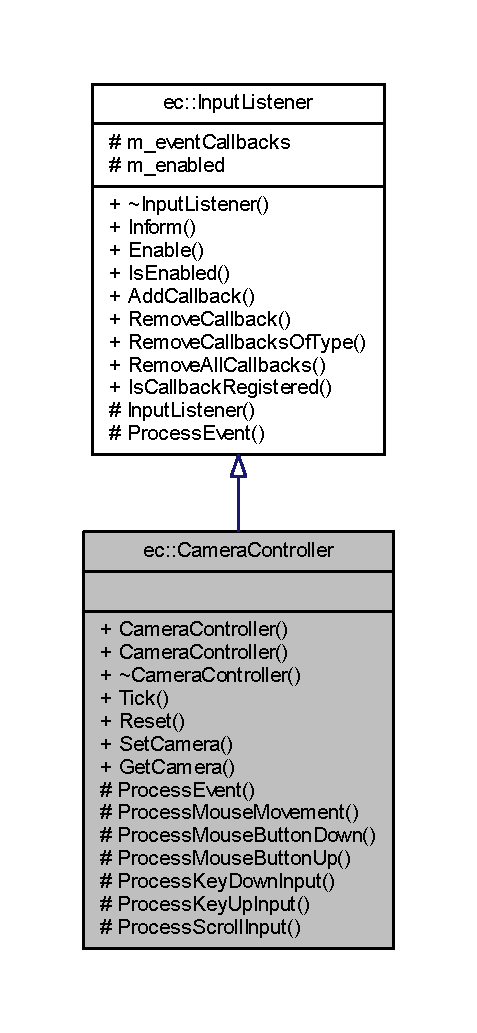
\includegraphics[width=227pt]{classec_1_1_camera_controller__inherit__graph}
\end{center}
\end{figure}


Collaboration diagram for ec\+:\+:Camera\+Controller\+:\nopagebreak
\begin{figure}[H]
\begin{center}
\leavevmode
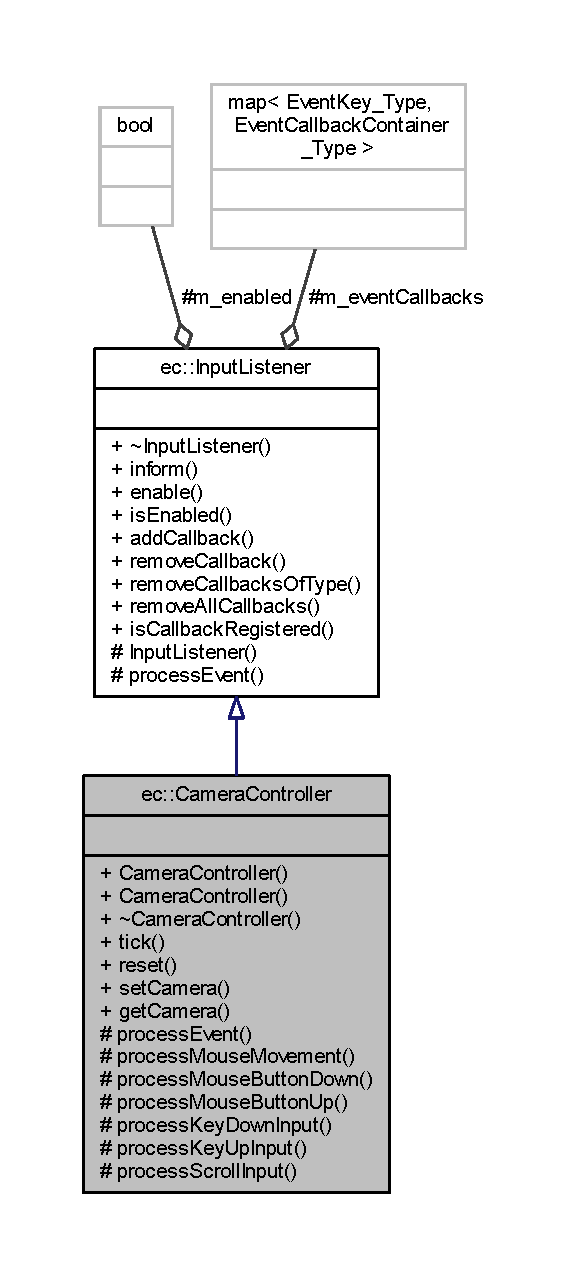
\includegraphics[height=550pt]{classec_1_1_camera_controller__coll__graph}
\end{center}
\end{figure}
\subsection*{Public Member Functions}
\begin{DoxyCompactItemize}
\item 
\mbox{\hyperlink{classec_1_1_camera_controller_a53fd061c49374fd8f1194cecac1e35aa}{Camera\+Controller}} ()
\item 
\mbox{\hyperlink{classec_1_1_camera_controller_a9edd8fff13533c84c7ea8f7f10f16580}{Camera\+Controller}} (\mbox{\hyperlink{classec_1_1_camera}{Camera}} $\ast$camera)
\item 
\mbox{\hyperlink{classec_1_1_camera_controller_a3229bd664f0d7d00b90fc3c9a852768c}{$\sim$\+Camera\+Controller}} ()
\item 
void \mbox{\hyperlink{classec_1_1_camera_controller_a82055ad6c8797937a8ec17234ab08758}{tick}} (float time\+Delta)
\begin{DoxyCompactList}\small\item\em Apply camera movement. \end{DoxyCompactList}\item 
void \mbox{\hyperlink{classec_1_1_camera_controller_a10d1642f398f155fa06c4c74961fe91f}{reset}} ()
\begin{DoxyCompactList}\small\item\em Reset camera to initial state. \end{DoxyCompactList}\item 
void \mbox{\hyperlink{classec_1_1_camera_controller_a74d3b80913b69dce0bae61a651c3b49b}{set\+Camera}} (\mbox{\hyperlink{classec_1_1_camera}{Camera}} $\ast$camera)
\begin{DoxyCompactList}\small\item\em Set the currently controlled camera. \end{DoxyCompactList}\item 
\mbox{\hyperlink{classec_1_1_camera}{Camera}} $\ast$ \mbox{\hyperlink{classec_1_1_camera_controller_a8d6e5c646108c0bf5abc25df3dd77c38}{get\+Camera}} () const
\end{DoxyCompactItemize}
\subsection*{Protected Member Functions}
\begin{DoxyCompactItemize}
\item 
void \mbox{\hyperlink{classec_1_1_camera_controller_af44aad5f80005eaadf5d637b3b00c6d6}{process\+Event}} (const \mbox{\hyperlink{structec_1_1_input_event}{Input\+Event}} \&event) override
\begin{DoxyCompactList}\small\item\em Process event to update camera movement. \end{DoxyCompactList}\item 
void \mbox{\hyperlink{classec_1_1_camera_controller_a9dc1490128a5946521a4111938564b42}{process\+Mouse\+Movement}} (const \mbox{\hyperlink{structec_1_1_mouse_event}{Mouse\+Event}} \&event)
\begin{DoxyCompactList}\small\item\em Used to rotate the camera with a mouse. \end{DoxyCompactList}\item 
void \mbox{\hyperlink{classec_1_1_camera_controller_ac2d7bd60346a2f23f591b9b5c05550dc}{process\+Mouse\+Button\+Down}} (const \mbox{\hyperlink{structec_1_1_mouse_event}{Mouse\+Event}} \&event)
\begin{DoxyCompactList}\small\item\em Enables camera rotation by mouse. \end{DoxyCompactList}\item 
void \mbox{\hyperlink{classec_1_1_camera_controller_af2a0f763157a655d53538ac9644620dd}{process\+Mouse\+Button\+Up}} (const \mbox{\hyperlink{structec_1_1_mouse_event}{Mouse\+Event}} \&event)
\begin{DoxyCompactList}\small\item\em Disables camera rotation by mouse. \end{DoxyCompactList}\item 
void \mbox{\hyperlink{classec_1_1_camera_controller_af1e6f226b4af2aa815bd885f71d25c12}{process\+Key\+Down\+Input}} (const \mbox{\hyperlink{structec_1_1_keyboard_event}{Keyboard\+Event}} \&event)
\begin{DoxyCompactList}\small\item\em Enable linear movement. \end{DoxyCompactList}\item 
void \mbox{\hyperlink{classec_1_1_camera_controller_ac92bb03a95ddf600b4a08b5b043b601e}{process\+Key\+Up\+Input}} (const \mbox{\hyperlink{structec_1_1_keyboard_event}{Keyboard\+Event}} \&event)
\begin{DoxyCompactList}\small\item\em Disable linear movement. \end{DoxyCompactList}\item 
void \mbox{\hyperlink{classec_1_1_camera_controller_aa2f60cde89ba3e982eef28d505927c22}{process\+Scroll\+Input}} (const \mbox{\hyperlink{structec_1_1_mouse_event}{Mouse\+Event}} \&event) const
\begin{DoxyCompactList}\small\item\em Change fov. \end{DoxyCompactList}\end{DoxyCompactItemize}
\subsection*{Additional Inherited Members}


\subsection{Constructor \& Destructor Documentation}
\mbox{\Hypertarget{classec_1_1_camera_controller_a53fd061c49374fd8f1194cecac1e35aa}\label{classec_1_1_camera_controller_a53fd061c49374fd8f1194cecac1e35aa}} 
\index{ec\+::\+Camera\+Controller@{ec\+::\+Camera\+Controller}!Camera\+Controller@{Camera\+Controller}}
\index{Camera\+Controller@{Camera\+Controller}!ec\+::\+Camera\+Controller@{ec\+::\+Camera\+Controller}}
\subsubsection{\texorpdfstring{Camera\+Controller()}{CameraController()}\hspace{0.1cm}{\footnotesize\ttfamily [1/2]}}
{\footnotesize\ttfamily ec\+::\+Camera\+Controller\+::\+Camera\+Controller (\begin{DoxyParamCaption}{ }\end{DoxyParamCaption})\hspace{0.3cm}{\ttfamily [explicit]}}

\mbox{\Hypertarget{classec_1_1_camera_controller_a9edd8fff13533c84c7ea8f7f10f16580}\label{classec_1_1_camera_controller_a9edd8fff13533c84c7ea8f7f10f16580}} 
\index{ec\+::\+Camera\+Controller@{ec\+::\+Camera\+Controller}!Camera\+Controller@{Camera\+Controller}}
\index{Camera\+Controller@{Camera\+Controller}!ec\+::\+Camera\+Controller@{ec\+::\+Camera\+Controller}}
\subsubsection{\texorpdfstring{Camera\+Controller()}{CameraController()}\hspace{0.1cm}{\footnotesize\ttfamily [2/2]}}
{\footnotesize\ttfamily ec\+::\+Camera\+Controller\+::\+Camera\+Controller (\begin{DoxyParamCaption}\item[{\mbox{\hyperlink{classec_1_1_camera}{Camera}} $\ast$}]{camera }\end{DoxyParamCaption})\hspace{0.3cm}{\ttfamily [explicit]}}

\mbox{\Hypertarget{classec_1_1_camera_controller_a3229bd664f0d7d00b90fc3c9a852768c}\label{classec_1_1_camera_controller_a3229bd664f0d7d00b90fc3c9a852768c}} 
\index{ec\+::\+Camera\+Controller@{ec\+::\+Camera\+Controller}!````~Camera\+Controller@{$\sim$\+Camera\+Controller}}
\index{````~Camera\+Controller@{$\sim$\+Camera\+Controller}!ec\+::\+Camera\+Controller@{ec\+::\+Camera\+Controller}}
\subsubsection{\texorpdfstring{$\sim$\+Camera\+Controller()}{~CameraController()}}
{\footnotesize\ttfamily ec\+::\+Camera\+Controller\+::$\sim$\+Camera\+Controller (\begin{DoxyParamCaption}{ }\end{DoxyParamCaption})\hspace{0.3cm}{\ttfamily [default]}}



\subsection{Member Function Documentation}
\mbox{\Hypertarget{classec_1_1_camera_controller_a8d6e5c646108c0bf5abc25df3dd77c38}\label{classec_1_1_camera_controller_a8d6e5c646108c0bf5abc25df3dd77c38}} 
\index{ec\+::\+Camera\+Controller@{ec\+::\+Camera\+Controller}!get\+Camera@{get\+Camera}}
\index{get\+Camera@{get\+Camera}!ec\+::\+Camera\+Controller@{ec\+::\+Camera\+Controller}}
\subsubsection{\texorpdfstring{get\+Camera()}{getCamera()}}
{\footnotesize\ttfamily \mbox{\hyperlink{classec_1_1_camera}{ec\+::\+Camera}} $\ast$ ec\+::\+Camera\+Controller\+::get\+Camera (\begin{DoxyParamCaption}{ }\end{DoxyParamCaption}) const}

\begin{DoxyReturn}{Returns}
The currently controlled camera. 
\end{DoxyReturn}
\mbox{\Hypertarget{classec_1_1_camera_controller_af44aad5f80005eaadf5d637b3b00c6d6}\label{classec_1_1_camera_controller_af44aad5f80005eaadf5d637b3b00c6d6}} 
\index{ec\+::\+Camera\+Controller@{ec\+::\+Camera\+Controller}!process\+Event@{process\+Event}}
\index{process\+Event@{process\+Event}!ec\+::\+Camera\+Controller@{ec\+::\+Camera\+Controller}}
\subsubsection{\texorpdfstring{process\+Event()}{processEvent()}}
{\footnotesize\ttfamily void ec\+::\+Camera\+Controller\+::process\+Event (\begin{DoxyParamCaption}\item[{const \mbox{\hyperlink{structec_1_1_input_event}{Input\+Event}} \&}]{event }\end{DoxyParamCaption})\hspace{0.3cm}{\ttfamily [override]}, {\ttfamily [protected]}, {\ttfamily [virtual]}}



Process event to update camera movement. 


\begin{DoxyParams}{Parameters}
{\em event} & An input event. \\
\hline
\end{DoxyParams}


Reimplemented from \mbox{\hyperlink{classec_1_1_input_listener_a9ceaefc79c6b0b260e88454616137840}{ec\+::\+Input\+Listener}}.

\mbox{\Hypertarget{classec_1_1_camera_controller_af1e6f226b4af2aa815bd885f71d25c12}\label{classec_1_1_camera_controller_af1e6f226b4af2aa815bd885f71d25c12}} 
\index{ec\+::\+Camera\+Controller@{ec\+::\+Camera\+Controller}!process\+Key\+Down\+Input@{process\+Key\+Down\+Input}}
\index{process\+Key\+Down\+Input@{process\+Key\+Down\+Input}!ec\+::\+Camera\+Controller@{ec\+::\+Camera\+Controller}}
\subsubsection{\texorpdfstring{process\+Key\+Down\+Input()}{processKeyDownInput()}}
{\footnotesize\ttfamily void ec\+::\+Camera\+Controller\+::process\+Key\+Down\+Input (\begin{DoxyParamCaption}\item[{const \mbox{\hyperlink{structec_1_1_keyboard_event}{Keyboard\+Event}} \&}]{event }\end{DoxyParamCaption})\hspace{0.3cm}{\ttfamily [protected]}}



Enable linear movement. 

\mbox{\Hypertarget{classec_1_1_camera_controller_ac92bb03a95ddf600b4a08b5b043b601e}\label{classec_1_1_camera_controller_ac92bb03a95ddf600b4a08b5b043b601e}} 
\index{ec\+::\+Camera\+Controller@{ec\+::\+Camera\+Controller}!process\+Key\+Up\+Input@{process\+Key\+Up\+Input}}
\index{process\+Key\+Up\+Input@{process\+Key\+Up\+Input}!ec\+::\+Camera\+Controller@{ec\+::\+Camera\+Controller}}
\subsubsection{\texorpdfstring{process\+Key\+Up\+Input()}{processKeyUpInput()}}
{\footnotesize\ttfamily void ec\+::\+Camera\+Controller\+::process\+Key\+Up\+Input (\begin{DoxyParamCaption}\item[{const \mbox{\hyperlink{structec_1_1_keyboard_event}{Keyboard\+Event}} \&}]{event }\end{DoxyParamCaption})\hspace{0.3cm}{\ttfamily [protected]}}



Disable linear movement. 

\mbox{\Hypertarget{classec_1_1_camera_controller_ac2d7bd60346a2f23f591b9b5c05550dc}\label{classec_1_1_camera_controller_ac2d7bd60346a2f23f591b9b5c05550dc}} 
\index{ec\+::\+Camera\+Controller@{ec\+::\+Camera\+Controller}!process\+Mouse\+Button\+Down@{process\+Mouse\+Button\+Down}}
\index{process\+Mouse\+Button\+Down@{process\+Mouse\+Button\+Down}!ec\+::\+Camera\+Controller@{ec\+::\+Camera\+Controller}}
\subsubsection{\texorpdfstring{process\+Mouse\+Button\+Down()}{processMouseButtonDown()}}
{\footnotesize\ttfamily void ec\+::\+Camera\+Controller\+::process\+Mouse\+Button\+Down (\begin{DoxyParamCaption}\item[{const \mbox{\hyperlink{structec_1_1_mouse_event}{Mouse\+Event}} \&}]{event }\end{DoxyParamCaption})\hspace{0.3cm}{\ttfamily [protected]}}



Enables camera rotation by mouse. 

\mbox{\Hypertarget{classec_1_1_camera_controller_af2a0f763157a655d53538ac9644620dd}\label{classec_1_1_camera_controller_af2a0f763157a655d53538ac9644620dd}} 
\index{ec\+::\+Camera\+Controller@{ec\+::\+Camera\+Controller}!process\+Mouse\+Button\+Up@{process\+Mouse\+Button\+Up}}
\index{process\+Mouse\+Button\+Up@{process\+Mouse\+Button\+Up}!ec\+::\+Camera\+Controller@{ec\+::\+Camera\+Controller}}
\subsubsection{\texorpdfstring{process\+Mouse\+Button\+Up()}{processMouseButtonUp()}}
{\footnotesize\ttfamily void ec\+::\+Camera\+Controller\+::process\+Mouse\+Button\+Up (\begin{DoxyParamCaption}\item[{const \mbox{\hyperlink{structec_1_1_mouse_event}{Mouse\+Event}} \&}]{event }\end{DoxyParamCaption})\hspace{0.3cm}{\ttfamily [protected]}}



Disables camera rotation by mouse. 

\mbox{\Hypertarget{classec_1_1_camera_controller_a9dc1490128a5946521a4111938564b42}\label{classec_1_1_camera_controller_a9dc1490128a5946521a4111938564b42}} 
\index{ec\+::\+Camera\+Controller@{ec\+::\+Camera\+Controller}!process\+Mouse\+Movement@{process\+Mouse\+Movement}}
\index{process\+Mouse\+Movement@{process\+Mouse\+Movement}!ec\+::\+Camera\+Controller@{ec\+::\+Camera\+Controller}}
\subsubsection{\texorpdfstring{process\+Mouse\+Movement()}{processMouseMovement()}}
{\footnotesize\ttfamily void ec\+::\+Camera\+Controller\+::process\+Mouse\+Movement (\begin{DoxyParamCaption}\item[{const \mbox{\hyperlink{structec_1_1_mouse_event}{Mouse\+Event}} \&}]{event }\end{DoxyParamCaption})\hspace{0.3cm}{\ttfamily [protected]}}



Used to rotate the camera with a mouse. 

\mbox{\Hypertarget{classec_1_1_camera_controller_aa2f60cde89ba3e982eef28d505927c22}\label{classec_1_1_camera_controller_aa2f60cde89ba3e982eef28d505927c22}} 
\index{ec\+::\+Camera\+Controller@{ec\+::\+Camera\+Controller}!process\+Scroll\+Input@{process\+Scroll\+Input}}
\index{process\+Scroll\+Input@{process\+Scroll\+Input}!ec\+::\+Camera\+Controller@{ec\+::\+Camera\+Controller}}
\subsubsection{\texorpdfstring{process\+Scroll\+Input()}{processScrollInput()}}
{\footnotesize\ttfamily void ec\+::\+Camera\+Controller\+::process\+Scroll\+Input (\begin{DoxyParamCaption}\item[{const \mbox{\hyperlink{structec_1_1_mouse_event}{Mouse\+Event}} \&}]{event }\end{DoxyParamCaption}) const\hspace{0.3cm}{\ttfamily [protected]}}



Change fov. 

\mbox{\Hypertarget{classec_1_1_camera_controller_a10d1642f398f155fa06c4c74961fe91f}\label{classec_1_1_camera_controller_a10d1642f398f155fa06c4c74961fe91f}} 
\index{ec\+::\+Camera\+Controller@{ec\+::\+Camera\+Controller}!reset@{reset}}
\index{reset@{reset}!ec\+::\+Camera\+Controller@{ec\+::\+Camera\+Controller}}
\subsubsection{\texorpdfstring{reset()}{reset()}}
{\footnotesize\ttfamily void ec\+::\+Camera\+Controller\+::reset (\begin{DoxyParamCaption}{ }\end{DoxyParamCaption})}



Reset camera to initial state. 

\mbox{\Hypertarget{classec_1_1_camera_controller_a74d3b80913b69dce0bae61a651c3b49b}\label{classec_1_1_camera_controller_a74d3b80913b69dce0bae61a651c3b49b}} 
\index{ec\+::\+Camera\+Controller@{ec\+::\+Camera\+Controller}!set\+Camera@{set\+Camera}}
\index{set\+Camera@{set\+Camera}!ec\+::\+Camera\+Controller@{ec\+::\+Camera\+Controller}}
\subsubsection{\texorpdfstring{set\+Camera()}{setCamera()}}
{\footnotesize\ttfamily void ec\+::\+Camera\+Controller\+::set\+Camera (\begin{DoxyParamCaption}\item[{\mbox{\hyperlink{classec_1_1_camera}{Camera}} $\ast$}]{camera }\end{DoxyParamCaption})}



Set the currently controlled camera. 

\mbox{\Hypertarget{classec_1_1_camera_controller_a82055ad6c8797937a8ec17234ab08758}\label{classec_1_1_camera_controller_a82055ad6c8797937a8ec17234ab08758}} 
\index{ec\+::\+Camera\+Controller@{ec\+::\+Camera\+Controller}!tick@{tick}}
\index{tick@{tick}!ec\+::\+Camera\+Controller@{ec\+::\+Camera\+Controller}}
\subsubsection{\texorpdfstring{tick()}{tick()}}
{\footnotesize\ttfamily void ec\+::\+Camera\+Controller\+::tick (\begin{DoxyParamCaption}\item[{float}]{time\+Delta }\end{DoxyParamCaption})}



Apply camera movement. 



The documentation for this class was generated from the following files\+:\begin{DoxyCompactItemize}
\item 
D\+:/\+Library/\+Documents/\+Job/\+Forschungsmaster/\+Projekte/\+Simulation\+Visualization/\+Eye\+Candy3\+D/\+Eye\+Candy3\+D/include/\+E\+C3\+D/\+Core/\mbox{\hyperlink{_camera_controller_8h}{Camera\+Controller.\+h}}\item 
D\+:/\+Library/\+Documents/\+Job/\+Forschungsmaster/\+Projekte/\+Simulation\+Visualization/\+Eye\+Candy3\+D/\+Eye\+Candy3\+D/src/\+Core/\mbox{\hyperlink{_camera_controller_8cpp}{Camera\+Controller.\+cpp}}\end{DoxyCompactItemize}

\hypertarget{classngl__gui_1_1_checkbox}{}\section{ngl\+\_\+gui\+:\+:Checkbox Class Reference}
\label{classngl__gui_1_1_checkbox}\index{ngl\+\_\+gui\+::\+Checkbox@{ngl\+\_\+gui\+::\+Checkbox}}


{\ttfamily \#include $<$Checkbox.\+h$>$}



Inheritance diagram for ngl\+\_\+gui\+:\+:Checkbox\+:\nopagebreak
\begin{figure}[H]
\begin{center}
\leavevmode
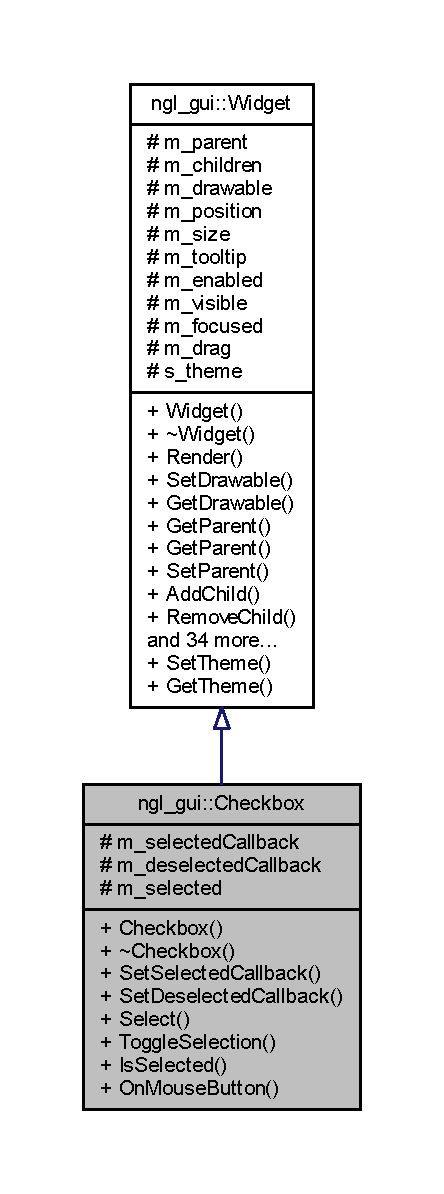
\includegraphics[height=550pt]{classngl__gui_1_1_checkbox__inherit__graph}
\end{center}
\end{figure}


Collaboration diagram for ngl\+\_\+gui\+:\+:Checkbox\+:
\nopagebreak
\begin{figure}[H]
\begin{center}
\leavevmode
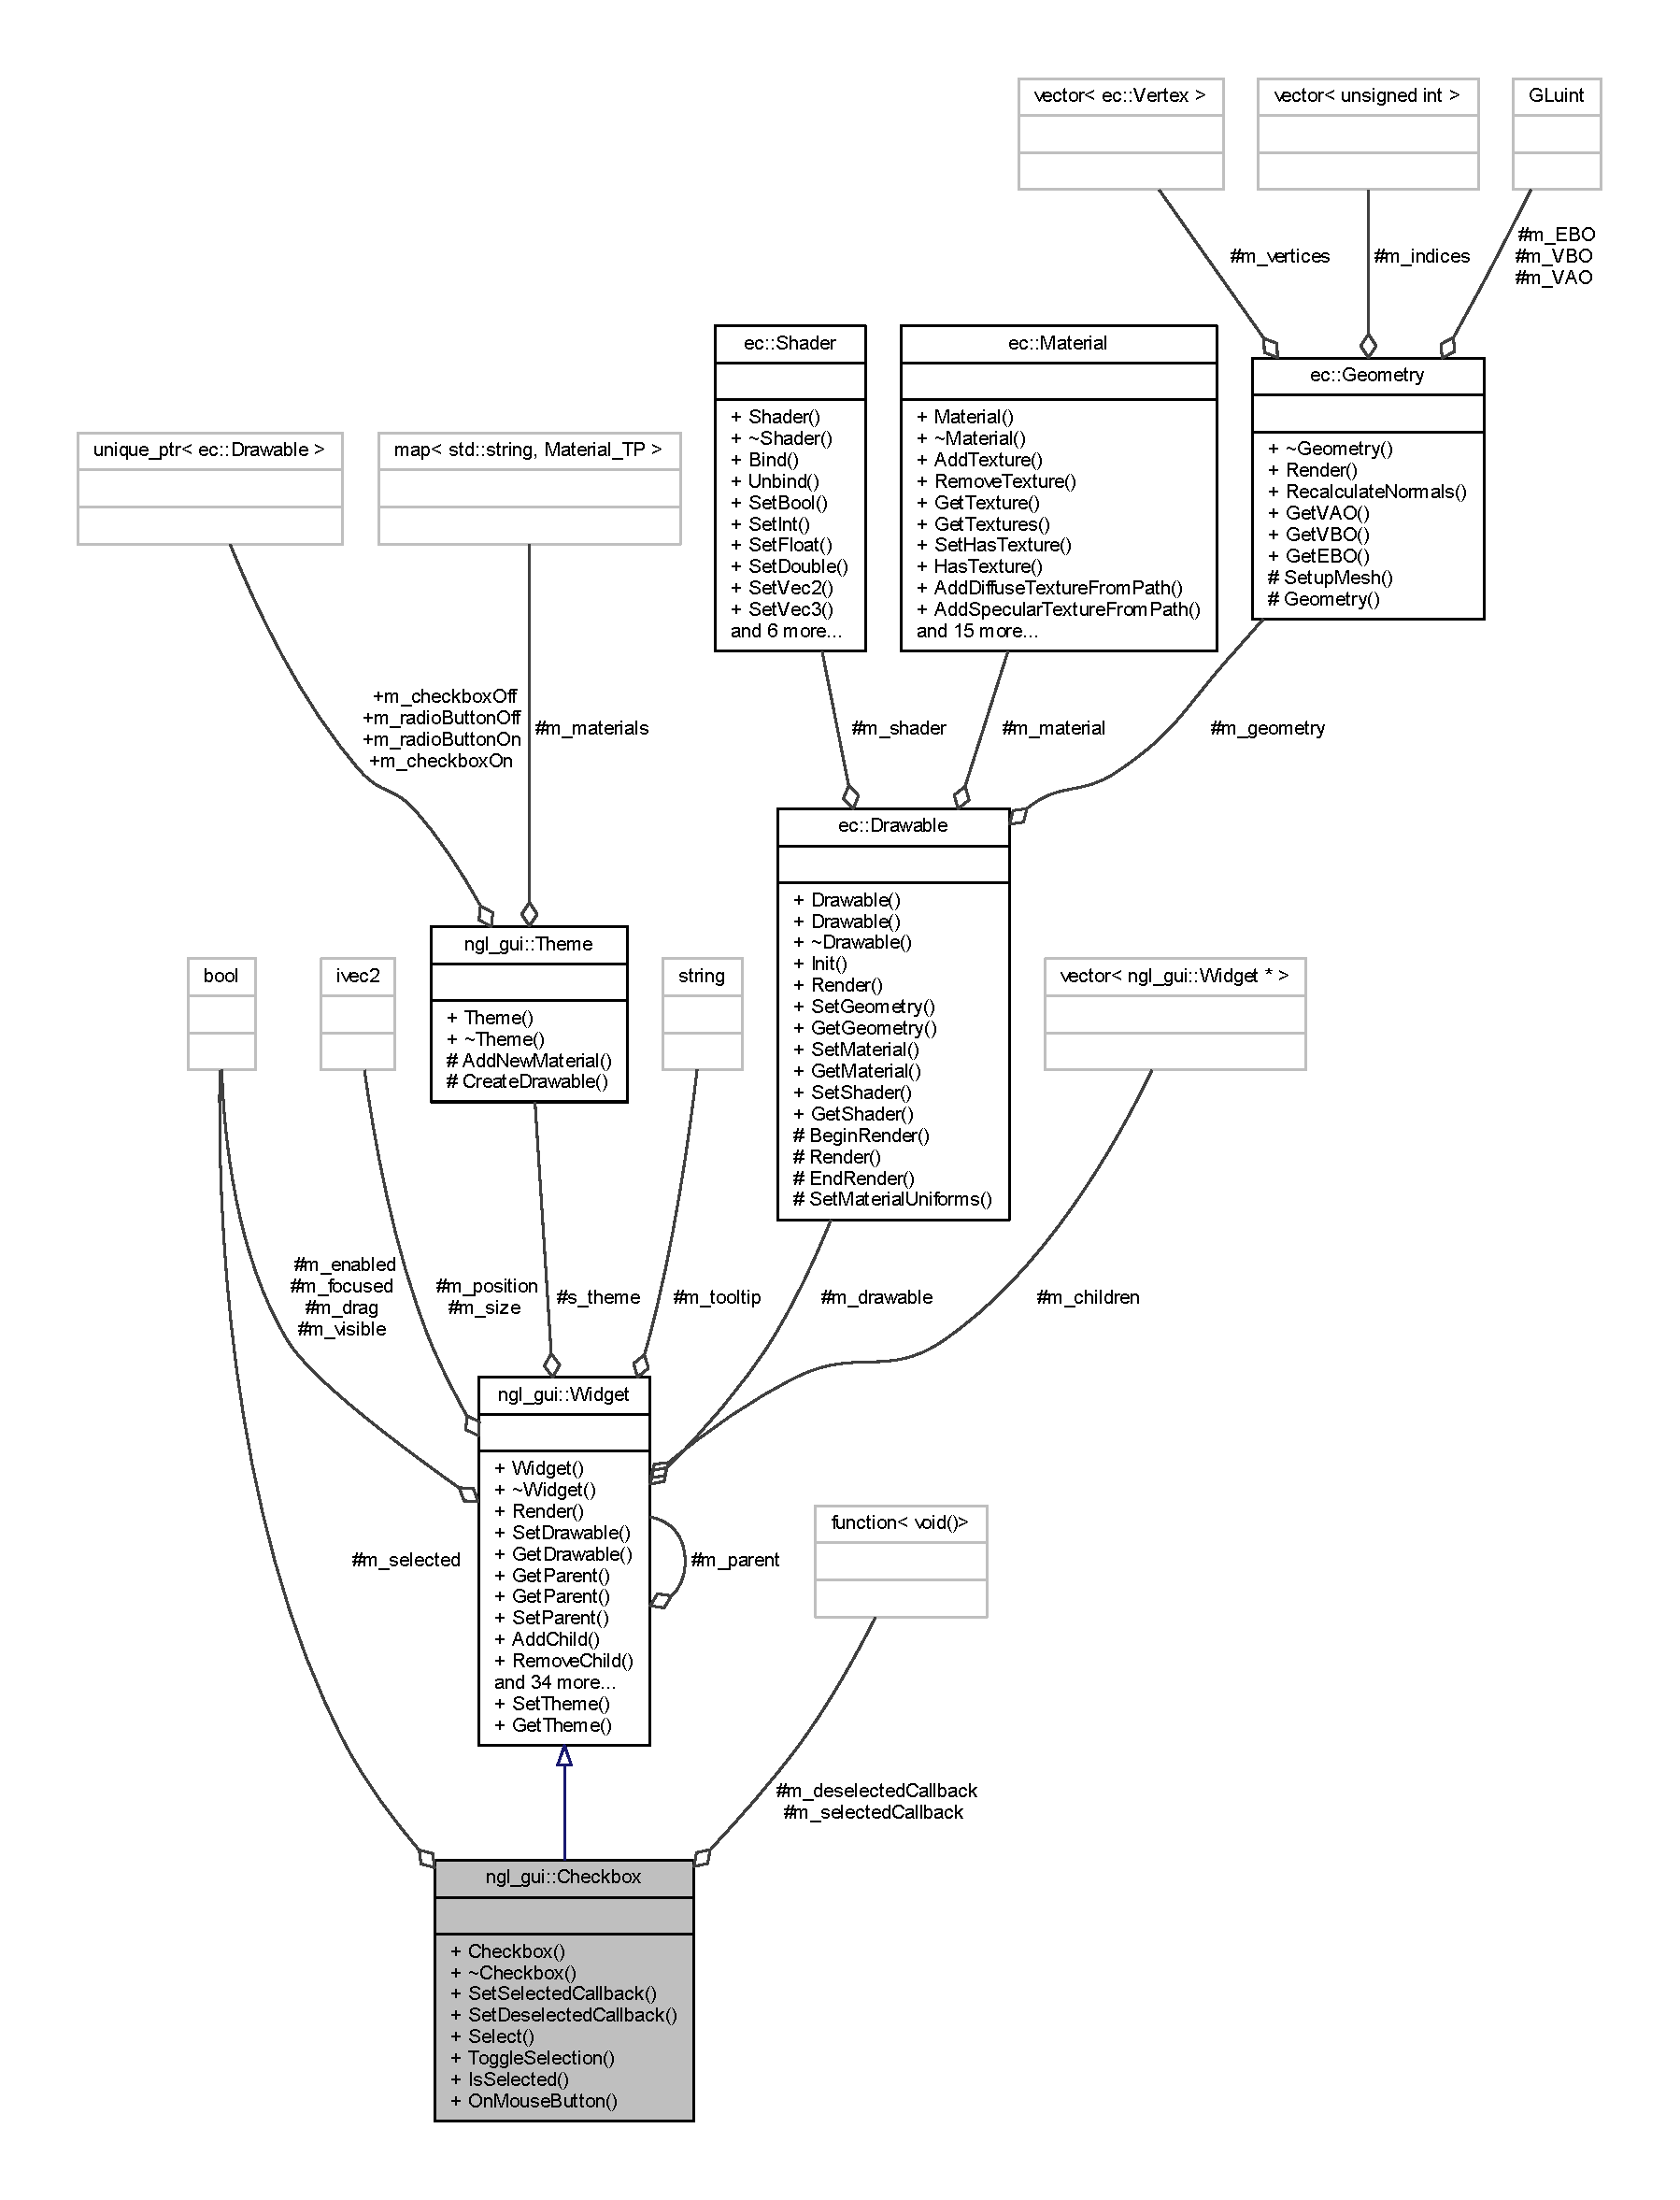
\includegraphics[width=350pt]{classngl__gui_1_1_checkbox__coll__graph}
\end{center}
\end{figure}
\subsection*{Public Member Functions}
\begin{DoxyCompactItemize}
\item 
\mbox{\hyperlink{classngl__gui_1_1_checkbox_adcc9cf43a4cff892c5e10bb41fe68777}{Checkbox}} (\mbox{\hyperlink{classngl__gui_1_1_widget}{Widget}} $\ast$parent)
\item 
virtual \mbox{\hyperlink{classngl__gui_1_1_checkbox_a31bdf168a6f602b81d8673db2317bdd4}{$\sim$\+Checkbox}} ()
\item 
void \mbox{\hyperlink{classngl__gui_1_1_checkbox_a09f0585a2fd2b73e15d1a755fa0d20c8}{Set\+Selected\+Callback}} (std\+::function$<$ void()$>$ callback)
\item 
void \mbox{\hyperlink{classngl__gui_1_1_checkbox_a1de9797b9fb31cb0e3f139f727224871}{Set\+Deselected\+Callback}} (std\+::function$<$ void()$>$ callback)
\item 
virtual void \mbox{\hyperlink{classngl__gui_1_1_checkbox_aa8045bf06c7121724c86083e5e5b166c}{Select}} (const bool selected)
\item 
virtual void \mbox{\hyperlink{classngl__gui_1_1_checkbox_a1cffeed17adcc790761916e4841a96d8}{Toggle\+Selection}} ()
\item 
bool \mbox{\hyperlink{classngl__gui_1_1_checkbox_a5352cab1a3b911eacb56422d41386390}{Is\+Selected}} () const
\item 
virtual bool \mbox{\hyperlink{classngl__gui_1_1_checkbox_a2616e2e230decef2a526e6fcfd59809e}{On\+Mouse\+Button}} (const glm\+::ivec2 \&position, int button, int mods, bool pressed) override
\end{DoxyCompactItemize}
\subsection*{Protected Attributes}
\begin{DoxyCompactItemize}
\item 
std\+::function$<$ void()$>$ \mbox{\hyperlink{classngl__gui_1_1_checkbox_a817578052ac5543eac703ba8e5f072c3}{m\+\_\+selected\+Callback}}
\item 
std\+::function$<$ void()$>$ \mbox{\hyperlink{classngl__gui_1_1_checkbox_aa2800070a32c1bd2137f1c16603e3883}{m\+\_\+deselected\+Callback}}
\item 
bool \mbox{\hyperlink{classngl__gui_1_1_checkbox_a218ceb62fd9ac89e1db17810f414984a}{m\+\_\+selected}}
\end{DoxyCompactItemize}
\subsection*{Additional Inherited Members}


\subsection{Constructor \& Destructor Documentation}
\mbox{\Hypertarget{classngl__gui_1_1_checkbox_adcc9cf43a4cff892c5e10bb41fe68777}\label{classngl__gui_1_1_checkbox_adcc9cf43a4cff892c5e10bb41fe68777}} 
\index{ngl\+\_\+gui\+::\+Checkbox@{ngl\+\_\+gui\+::\+Checkbox}!Checkbox@{Checkbox}}
\index{Checkbox@{Checkbox}!ngl\+\_\+gui\+::\+Checkbox@{ngl\+\_\+gui\+::\+Checkbox}}
\subsubsection{\texorpdfstring{Checkbox()}{Checkbox()}}
{\footnotesize\ttfamily ngl\+\_\+gui\+::\+Checkbox\+::\+Checkbox (\begin{DoxyParamCaption}\item[{\mbox{\hyperlink{classngl__gui_1_1_widget}{Widget}} $\ast$}]{parent }\end{DoxyParamCaption})\hspace{0.3cm}{\ttfamily [explicit]}}

\mbox{\Hypertarget{classngl__gui_1_1_checkbox_a31bdf168a6f602b81d8673db2317bdd4}\label{classngl__gui_1_1_checkbox_a31bdf168a6f602b81d8673db2317bdd4}} 
\index{ngl\+\_\+gui\+::\+Checkbox@{ngl\+\_\+gui\+::\+Checkbox}!````~Checkbox@{$\sim$\+Checkbox}}
\index{````~Checkbox@{$\sim$\+Checkbox}!ngl\+\_\+gui\+::\+Checkbox@{ngl\+\_\+gui\+::\+Checkbox}}
\subsubsection{\texorpdfstring{$\sim$\+Checkbox()}{~Checkbox()}}
{\footnotesize\ttfamily ngl\+\_\+gui\+::\+Checkbox\+::$\sim$\+Checkbox (\begin{DoxyParamCaption}{ }\end{DoxyParamCaption})\hspace{0.3cm}{\ttfamily [virtual]}}



\subsection{Member Function Documentation}
\mbox{\Hypertarget{classngl__gui_1_1_checkbox_a5352cab1a3b911eacb56422d41386390}\label{classngl__gui_1_1_checkbox_a5352cab1a3b911eacb56422d41386390}} 
\index{ngl\+\_\+gui\+::\+Checkbox@{ngl\+\_\+gui\+::\+Checkbox}!Is\+Selected@{Is\+Selected}}
\index{Is\+Selected@{Is\+Selected}!ngl\+\_\+gui\+::\+Checkbox@{ngl\+\_\+gui\+::\+Checkbox}}
\subsubsection{\texorpdfstring{Is\+Selected()}{IsSelected()}}
{\footnotesize\ttfamily bool ngl\+\_\+gui\+::\+Checkbox\+::\+Is\+Selected (\begin{DoxyParamCaption}{ }\end{DoxyParamCaption}) const}

\mbox{\Hypertarget{classngl__gui_1_1_checkbox_a2616e2e230decef2a526e6fcfd59809e}\label{classngl__gui_1_1_checkbox_a2616e2e230decef2a526e6fcfd59809e}} 
\index{ngl\+\_\+gui\+::\+Checkbox@{ngl\+\_\+gui\+::\+Checkbox}!On\+Mouse\+Button@{On\+Mouse\+Button}}
\index{On\+Mouse\+Button@{On\+Mouse\+Button}!ngl\+\_\+gui\+::\+Checkbox@{ngl\+\_\+gui\+::\+Checkbox}}
\subsubsection{\texorpdfstring{On\+Mouse\+Button()}{OnMouseButton()}}
{\footnotesize\ttfamily bool ngl\+\_\+gui\+::\+Checkbox\+::\+On\+Mouse\+Button (\begin{DoxyParamCaption}\item[{const glm\+::ivec2 \&}]{position,  }\item[{int}]{button,  }\item[{int}]{mods,  }\item[{bool}]{pressed }\end{DoxyParamCaption})\hspace{0.3cm}{\ttfamily [override]}, {\ttfamily [virtual]}}



Reimplemented from \mbox{\hyperlink{classngl__gui_1_1_widget_a721b18dc7a09b0b7b4ff0c02162409b8}{ngl\+\_\+gui\+::\+Widget}}.

\mbox{\Hypertarget{classngl__gui_1_1_checkbox_aa8045bf06c7121724c86083e5e5b166c}\label{classngl__gui_1_1_checkbox_aa8045bf06c7121724c86083e5e5b166c}} 
\index{ngl\+\_\+gui\+::\+Checkbox@{ngl\+\_\+gui\+::\+Checkbox}!Select@{Select}}
\index{Select@{Select}!ngl\+\_\+gui\+::\+Checkbox@{ngl\+\_\+gui\+::\+Checkbox}}
\subsubsection{\texorpdfstring{Select()}{Select()}}
{\footnotesize\ttfamily void ngl\+\_\+gui\+::\+Checkbox\+::\+Select (\begin{DoxyParamCaption}\item[{const bool}]{selected }\end{DoxyParamCaption})\hspace{0.3cm}{\ttfamily [virtual]}}

\mbox{\Hypertarget{classngl__gui_1_1_checkbox_a1de9797b9fb31cb0e3f139f727224871}\label{classngl__gui_1_1_checkbox_a1de9797b9fb31cb0e3f139f727224871}} 
\index{ngl\+\_\+gui\+::\+Checkbox@{ngl\+\_\+gui\+::\+Checkbox}!Set\+Deselected\+Callback@{Set\+Deselected\+Callback}}
\index{Set\+Deselected\+Callback@{Set\+Deselected\+Callback}!ngl\+\_\+gui\+::\+Checkbox@{ngl\+\_\+gui\+::\+Checkbox}}
\subsubsection{\texorpdfstring{Set\+Deselected\+Callback()}{SetDeselectedCallback()}}
{\footnotesize\ttfamily void ngl\+\_\+gui\+::\+Checkbox\+::\+Set\+Deselected\+Callback (\begin{DoxyParamCaption}\item[{std\+::function$<$ void()$>$}]{callback }\end{DoxyParamCaption})}

\mbox{\Hypertarget{classngl__gui_1_1_checkbox_a09f0585a2fd2b73e15d1a755fa0d20c8}\label{classngl__gui_1_1_checkbox_a09f0585a2fd2b73e15d1a755fa0d20c8}} 
\index{ngl\+\_\+gui\+::\+Checkbox@{ngl\+\_\+gui\+::\+Checkbox}!Set\+Selected\+Callback@{Set\+Selected\+Callback}}
\index{Set\+Selected\+Callback@{Set\+Selected\+Callback}!ngl\+\_\+gui\+::\+Checkbox@{ngl\+\_\+gui\+::\+Checkbox}}
\subsubsection{\texorpdfstring{Set\+Selected\+Callback()}{SetSelectedCallback()}}
{\footnotesize\ttfamily void ngl\+\_\+gui\+::\+Checkbox\+::\+Set\+Selected\+Callback (\begin{DoxyParamCaption}\item[{std\+::function$<$ void()$>$}]{callback }\end{DoxyParamCaption})}

\mbox{\Hypertarget{classngl__gui_1_1_checkbox_a1cffeed17adcc790761916e4841a96d8}\label{classngl__gui_1_1_checkbox_a1cffeed17adcc790761916e4841a96d8}} 
\index{ngl\+\_\+gui\+::\+Checkbox@{ngl\+\_\+gui\+::\+Checkbox}!Toggle\+Selection@{Toggle\+Selection}}
\index{Toggle\+Selection@{Toggle\+Selection}!ngl\+\_\+gui\+::\+Checkbox@{ngl\+\_\+gui\+::\+Checkbox}}
\subsubsection{\texorpdfstring{Toggle\+Selection()}{ToggleSelection()}}
{\footnotesize\ttfamily void ngl\+\_\+gui\+::\+Checkbox\+::\+Toggle\+Selection (\begin{DoxyParamCaption}{ }\end{DoxyParamCaption})\hspace{0.3cm}{\ttfamily [virtual]}}



\subsection{Member Data Documentation}
\mbox{\Hypertarget{classngl__gui_1_1_checkbox_aa2800070a32c1bd2137f1c16603e3883}\label{classngl__gui_1_1_checkbox_aa2800070a32c1bd2137f1c16603e3883}} 
\index{ngl\+\_\+gui\+::\+Checkbox@{ngl\+\_\+gui\+::\+Checkbox}!m\+\_\+deselected\+Callback@{m\+\_\+deselected\+Callback}}
\index{m\+\_\+deselected\+Callback@{m\+\_\+deselected\+Callback}!ngl\+\_\+gui\+::\+Checkbox@{ngl\+\_\+gui\+::\+Checkbox}}
\subsubsection{\texorpdfstring{m\+\_\+deselected\+Callback}{m\_deselectedCallback}}
{\footnotesize\ttfamily std\+::function$<$void()$>$ ngl\+\_\+gui\+::\+Checkbox\+::m\+\_\+deselected\+Callback\hspace{0.3cm}{\ttfamily [protected]}}

\mbox{\Hypertarget{classngl__gui_1_1_checkbox_a218ceb62fd9ac89e1db17810f414984a}\label{classngl__gui_1_1_checkbox_a218ceb62fd9ac89e1db17810f414984a}} 
\index{ngl\+\_\+gui\+::\+Checkbox@{ngl\+\_\+gui\+::\+Checkbox}!m\+\_\+selected@{m\+\_\+selected}}
\index{m\+\_\+selected@{m\+\_\+selected}!ngl\+\_\+gui\+::\+Checkbox@{ngl\+\_\+gui\+::\+Checkbox}}
\subsubsection{\texorpdfstring{m\+\_\+selected}{m\_selected}}
{\footnotesize\ttfamily bool ngl\+\_\+gui\+::\+Checkbox\+::m\+\_\+selected\hspace{0.3cm}{\ttfamily [protected]}}

\mbox{\Hypertarget{classngl__gui_1_1_checkbox_a817578052ac5543eac703ba8e5f072c3}\label{classngl__gui_1_1_checkbox_a817578052ac5543eac703ba8e5f072c3}} 
\index{ngl\+\_\+gui\+::\+Checkbox@{ngl\+\_\+gui\+::\+Checkbox}!m\+\_\+selected\+Callback@{m\+\_\+selected\+Callback}}
\index{m\+\_\+selected\+Callback@{m\+\_\+selected\+Callback}!ngl\+\_\+gui\+::\+Checkbox@{ngl\+\_\+gui\+::\+Checkbox}}
\subsubsection{\texorpdfstring{m\+\_\+selected\+Callback}{m\_selectedCallback}}
{\footnotesize\ttfamily std\+::function$<$void()$>$ ngl\+\_\+gui\+::\+Checkbox\+::m\+\_\+selected\+Callback\hspace{0.3cm}{\ttfamily [protected]}}



The documentation for this class was generated from the following files\+:\begin{DoxyCompactItemize}
\item 
D\+:/\+Library/\+Documents/\+Job/\+Forschungsmaster/\+Projekte/\+Eye\+Candy3\+D/\+Eye\+Candy3\+D/include/\+E\+C3\+D/\+G\+U\+I/\mbox{\hyperlink{_checkbox_8h}{Checkbox.\+h}}\item 
D\+:/\+Library/\+Documents/\+Job/\+Forschungsmaster/\+Projekte/\+Eye\+Candy3\+D/\+Eye\+Candy3\+D/src/\+G\+U\+I/\mbox{\hyperlink{_checkbox_8cpp}{Checkbox.\+cpp}}\end{DoxyCompactItemize}

\hypertarget{structec_1_1_closed_event}{}\section{ec\+:\+:Closed\+Event Struct Reference}
\label{structec_1_1_closed_event}\index{ec\+::\+Closed\+Event@{ec\+::\+Closed\+Event}}


{\ttfamily \#include $<$Input\+Event.\+h$>$}



Collaboration diagram for ec\+:\+:Closed\+Event\+:\nopagebreak
\begin{figure}[H]
\begin{center}
\leavevmode
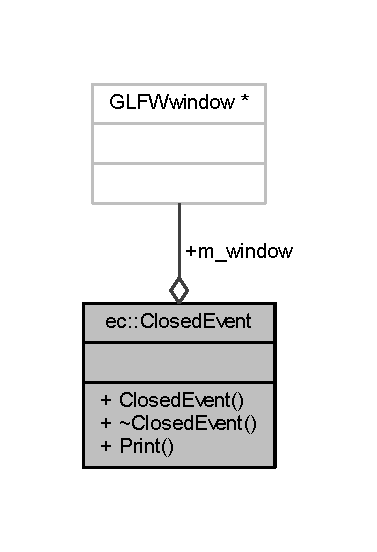
\includegraphics[width=181pt]{structec_1_1_closed_event__coll__graph}
\end{center}
\end{figure}
\subsection*{Public Member Functions}
\begin{DoxyCompactItemize}
\item 
\mbox{\hyperlink{structec_1_1_closed_event_a70ac7681a32c7abbc97add221d7d9477}{Closed\+Event}} (G\+L\+F\+Wwindow $\ast$window)
\item 
\mbox{\hyperlink{structec_1_1_closed_event_a59918a40f5034b5ece54db3d16900f31}{$\sim$\+Closed\+Event}} ()
\item 
void \mbox{\hyperlink{structec_1_1_closed_event_aa40d7f2ab8263bedc927d289a4a20190}{Print}} () const
\end{DoxyCompactItemize}
\subsection*{Public Attributes}
\begin{DoxyCompactItemize}
\item 
G\+L\+F\+Wwindow $\ast$ \mbox{\hyperlink{structec_1_1_closed_event_acd70453a645b12b21857e4e3a47f1294}{m\+\_\+window}}
\end{DoxyCompactItemize}


\subsection{Constructor \& Destructor Documentation}
\mbox{\Hypertarget{structec_1_1_closed_event_a70ac7681a32c7abbc97add221d7d9477}\label{structec_1_1_closed_event_a70ac7681a32c7abbc97add221d7d9477}} 
\index{ec\+::\+Closed\+Event@{ec\+::\+Closed\+Event}!Closed\+Event@{Closed\+Event}}
\index{Closed\+Event@{Closed\+Event}!ec\+::\+Closed\+Event@{ec\+::\+Closed\+Event}}
\subsubsection{\texorpdfstring{Closed\+Event()}{ClosedEvent()}}
{\footnotesize\ttfamily ec\+::\+Closed\+Event\+::\+Closed\+Event (\begin{DoxyParamCaption}\item[{G\+L\+F\+Wwindow $\ast$}]{window }\end{DoxyParamCaption})}

\mbox{\Hypertarget{structec_1_1_closed_event_a59918a40f5034b5ece54db3d16900f31}\label{structec_1_1_closed_event_a59918a40f5034b5ece54db3d16900f31}} 
\index{ec\+::\+Closed\+Event@{ec\+::\+Closed\+Event}!````~Closed\+Event@{$\sim$\+Closed\+Event}}
\index{````~Closed\+Event@{$\sim$\+Closed\+Event}!ec\+::\+Closed\+Event@{ec\+::\+Closed\+Event}}
\subsubsection{\texorpdfstring{$\sim$\+Closed\+Event()}{~ClosedEvent()}}
{\footnotesize\ttfamily ec\+::\+Closed\+Event\+::$\sim$\+Closed\+Event (\begin{DoxyParamCaption}{ }\end{DoxyParamCaption})}



\subsection{Member Function Documentation}
\mbox{\Hypertarget{structec_1_1_closed_event_aa40d7f2ab8263bedc927d289a4a20190}\label{structec_1_1_closed_event_aa40d7f2ab8263bedc927d289a4a20190}} 
\index{ec\+::\+Closed\+Event@{ec\+::\+Closed\+Event}!Print@{Print}}
\index{Print@{Print}!ec\+::\+Closed\+Event@{ec\+::\+Closed\+Event}}
\subsubsection{\texorpdfstring{Print()}{Print()}}
{\footnotesize\ttfamily void ec\+::\+Closed\+Event\+::\+Print (\begin{DoxyParamCaption}{ }\end{DoxyParamCaption}) const}



\subsection{Member Data Documentation}
\mbox{\Hypertarget{structec_1_1_closed_event_acd70453a645b12b21857e4e3a47f1294}\label{structec_1_1_closed_event_acd70453a645b12b21857e4e3a47f1294}} 
\index{ec\+::\+Closed\+Event@{ec\+::\+Closed\+Event}!m\+\_\+window@{m\+\_\+window}}
\index{m\+\_\+window@{m\+\_\+window}!ec\+::\+Closed\+Event@{ec\+::\+Closed\+Event}}
\subsubsection{\texorpdfstring{m\+\_\+window}{m\_window}}
{\footnotesize\ttfamily G\+L\+F\+Wwindow$\ast$ ec\+::\+Closed\+Event\+::m\+\_\+window}



The documentation for this struct was generated from the following files\+:\begin{DoxyCompactItemize}
\item 
D\+:/\+Library/\+Documents/\+Job/\+Forschungsmaster/\+Projekte/\+Eye\+Candy3\+D/\+Eye\+Candy3\+D/include/\+E\+C3\+D/\+Core/\mbox{\hyperlink{_input_event_8h}{Input\+Event.\+h}}\item 
D\+:/\+Library/\+Documents/\+Job/\+Forschungsmaster/\+Projekte/\+Eye\+Candy3\+D/\+Eye\+Candy3\+D/src/\+Core/\mbox{\hyperlink{_input_event_8cpp}{Input\+Event.\+cpp}}\end{DoxyCompactItemize}

\hypertarget{classec_1_1_cube_mesh}{}\section{ec\+:\+:Cube\+Mesh Class Reference}
\label{classec_1_1_cube_mesh}\index{ec\+::\+Cube\+Mesh@{ec\+::\+Cube\+Mesh}}


{\ttfamily \#include $<$Cube\+Mesh.\+h$>$}



Inheritance diagram for ec\+:\+:Cube\+Mesh\+:\nopagebreak
\begin{figure}[H]
\begin{center}
\leavevmode
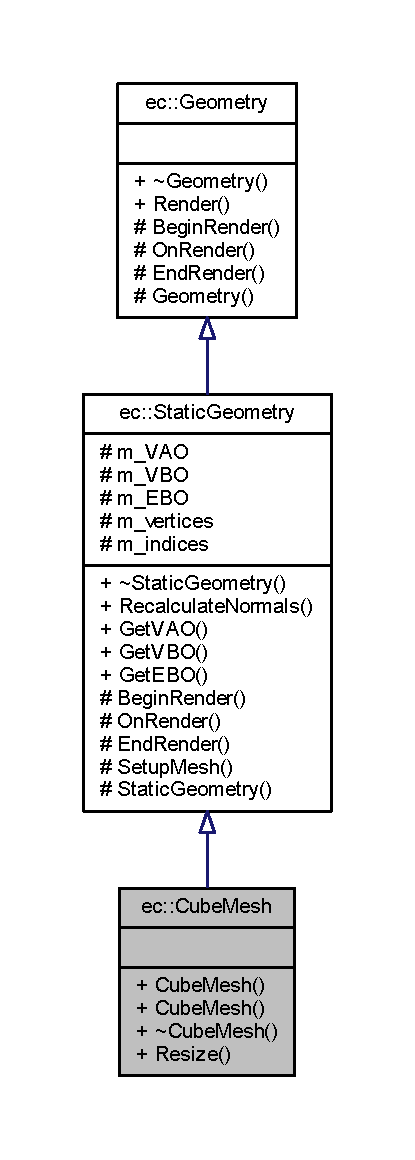
\includegraphics[width=199pt]{classec_1_1_cube_mesh__inherit__graph}
\end{center}
\end{figure}


Collaboration diagram for ec\+:\+:Cube\+Mesh\+:\nopagebreak
\begin{figure}[H]
\begin{center}
\leavevmode
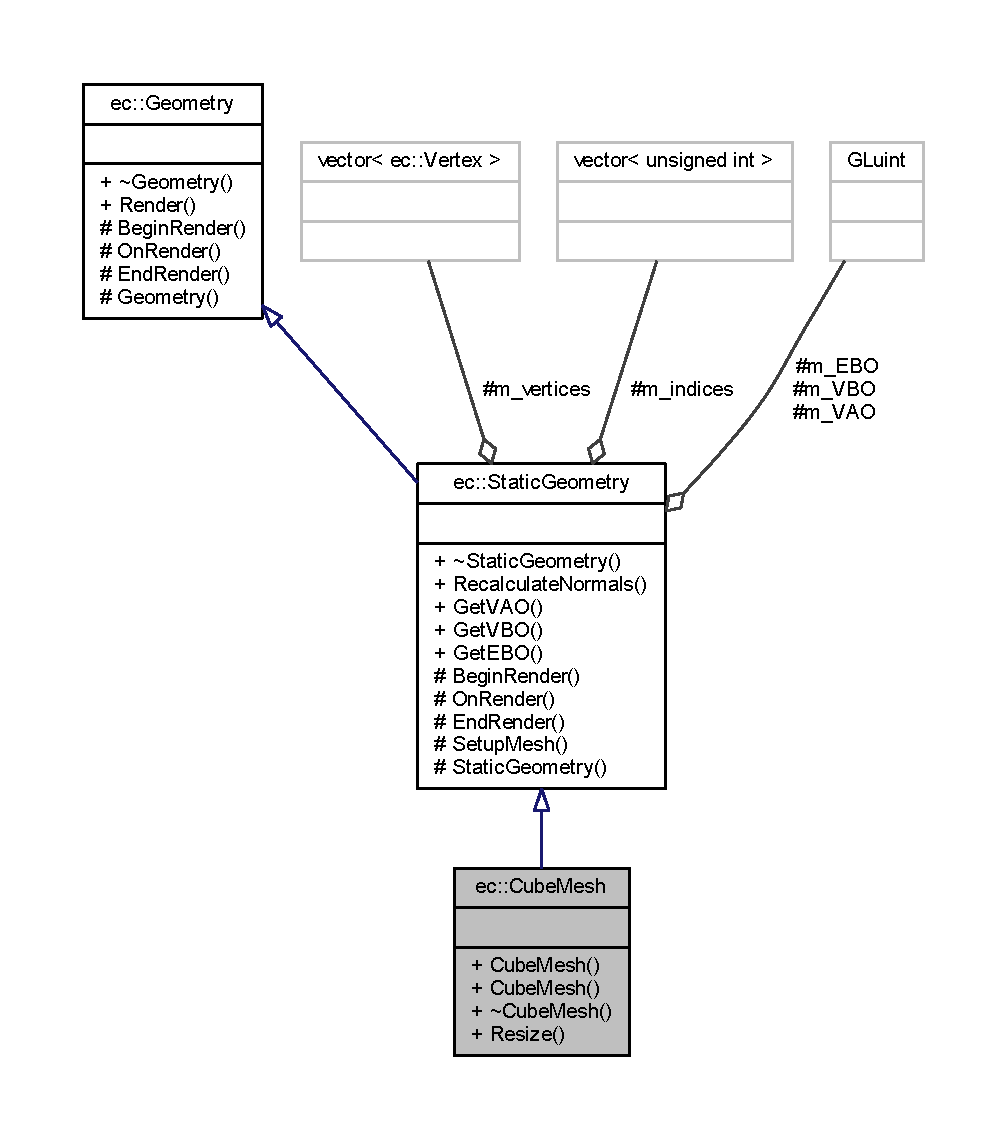
\includegraphics[width=350pt]{classec_1_1_cube_mesh__coll__graph}
\end{center}
\end{figure}
\subsection*{Public Member Functions}
\begin{DoxyCompactItemize}
\item 
\mbox{\hyperlink{classec_1_1_cube_mesh_ac7a03d63c5e3f57ef94e5d18098b4a03}{Cube\+Mesh}} (const float uniform\+Size=1.\+0f)
\item 
\mbox{\hyperlink{classec_1_1_cube_mesh_a645d007818631c7ab01c4725ec6818a6}{Cube\+Mesh}} (const float width, const float height, const float depth)
\item 
\mbox{\hyperlink{classec_1_1_cube_mesh_a59af4189ee0c7fa24e2bd239acc6589d}{$\sim$\+Cube\+Mesh}} ()
\item 
void \mbox{\hyperlink{classec_1_1_cube_mesh_a4c2538e7fa1de0ea96c794ae3bc6e1d7}{Resize}} (float width, float height, float depth)
\end{DoxyCompactItemize}
\subsection*{Additional Inherited Members}


\subsection{Constructor \& Destructor Documentation}
\mbox{\Hypertarget{classec_1_1_cube_mesh_ac7a03d63c5e3f57ef94e5d18098b4a03}\label{classec_1_1_cube_mesh_ac7a03d63c5e3f57ef94e5d18098b4a03}} 
\index{ec\+::\+Cube\+Mesh@{ec\+::\+Cube\+Mesh}!Cube\+Mesh@{Cube\+Mesh}}
\index{Cube\+Mesh@{Cube\+Mesh}!ec\+::\+Cube\+Mesh@{ec\+::\+Cube\+Mesh}}
\subsubsection{\texorpdfstring{Cube\+Mesh()}{CubeMesh()}\hspace{0.1cm}{\footnotesize\ttfamily [1/2]}}
{\footnotesize\ttfamily ec\+::\+Cube\+Mesh\+::\+Cube\+Mesh (\begin{DoxyParamCaption}\item[{const float}]{uniform\+Size = {\ttfamily 1.0f} }\end{DoxyParamCaption})\hspace{0.3cm}{\ttfamily [explicit]}}

\mbox{\Hypertarget{classec_1_1_cube_mesh_a645d007818631c7ab01c4725ec6818a6}\label{classec_1_1_cube_mesh_a645d007818631c7ab01c4725ec6818a6}} 
\index{ec\+::\+Cube\+Mesh@{ec\+::\+Cube\+Mesh}!Cube\+Mesh@{Cube\+Mesh}}
\index{Cube\+Mesh@{Cube\+Mesh}!ec\+::\+Cube\+Mesh@{ec\+::\+Cube\+Mesh}}
\subsubsection{\texorpdfstring{Cube\+Mesh()}{CubeMesh()}\hspace{0.1cm}{\footnotesize\ttfamily [2/2]}}
{\footnotesize\ttfamily ec\+::\+Cube\+Mesh\+::\+Cube\+Mesh (\begin{DoxyParamCaption}\item[{const float}]{width,  }\item[{const float}]{height,  }\item[{const float}]{depth }\end{DoxyParamCaption})\hspace{0.3cm}{\ttfamily [explicit]}}

\mbox{\Hypertarget{classec_1_1_cube_mesh_a59af4189ee0c7fa24e2bd239acc6589d}\label{classec_1_1_cube_mesh_a59af4189ee0c7fa24e2bd239acc6589d}} 
\index{ec\+::\+Cube\+Mesh@{ec\+::\+Cube\+Mesh}!````~Cube\+Mesh@{$\sim$\+Cube\+Mesh}}
\index{````~Cube\+Mesh@{$\sim$\+Cube\+Mesh}!ec\+::\+Cube\+Mesh@{ec\+::\+Cube\+Mesh}}
\subsubsection{\texorpdfstring{$\sim$\+Cube\+Mesh()}{~CubeMesh()}}
{\footnotesize\ttfamily ec\+::\+Cube\+Mesh\+::$\sim$\+Cube\+Mesh (\begin{DoxyParamCaption}{ }\end{DoxyParamCaption})}



\subsection{Member Function Documentation}
\mbox{\Hypertarget{classec_1_1_cube_mesh_a4c2538e7fa1de0ea96c794ae3bc6e1d7}\label{classec_1_1_cube_mesh_a4c2538e7fa1de0ea96c794ae3bc6e1d7}} 
\index{ec\+::\+Cube\+Mesh@{ec\+::\+Cube\+Mesh}!Resize@{Resize}}
\index{Resize@{Resize}!ec\+::\+Cube\+Mesh@{ec\+::\+Cube\+Mesh}}
\subsubsection{\texorpdfstring{Resize()}{Resize()}}
{\footnotesize\ttfamily void ec\+::\+Cube\+Mesh\+::\+Resize (\begin{DoxyParamCaption}\item[{float}]{width,  }\item[{float}]{height,  }\item[{float}]{depth }\end{DoxyParamCaption})}



The documentation for this class was generated from the following files\+:\begin{DoxyCompactItemize}
\item 
D\+:/\+Library/\+Documents/\+Job/\+Forschungsmaster/\+Projekte/\+Eye\+Candy3\+D/\+Eye\+Candy3\+D/include/\+E\+C3\+D/\+Core/\mbox{\hyperlink{_cube_mesh_8h}{Cube\+Mesh.\+h}}\item 
D\+:/\+Library/\+Documents/\+Job/\+Forschungsmaster/\+Projekte/\+Eye\+Candy3\+D/\+Eye\+Candy3\+D/src/\+Core/\mbox{\hyperlink{_cube_mesh_8cpp}{Cube\+Mesh.\+cpp}}\end{DoxyCompactItemize}

\hypertarget{classec_1_1_drawable}{}\section{ec\+:\+:Drawable Class Reference}
\label{classec_1_1_drawable}\index{ec\+::\+Drawable@{ec\+::\+Drawable}}


Core class for rendering geometry data with a certain material and shader.  




{\ttfamily \#include $<$Drawable.\+h$>$}



Collaboration diagram for ec\+:\+:Drawable\+:\nopagebreak
\begin{figure}[H]
\begin{center}
\leavevmode
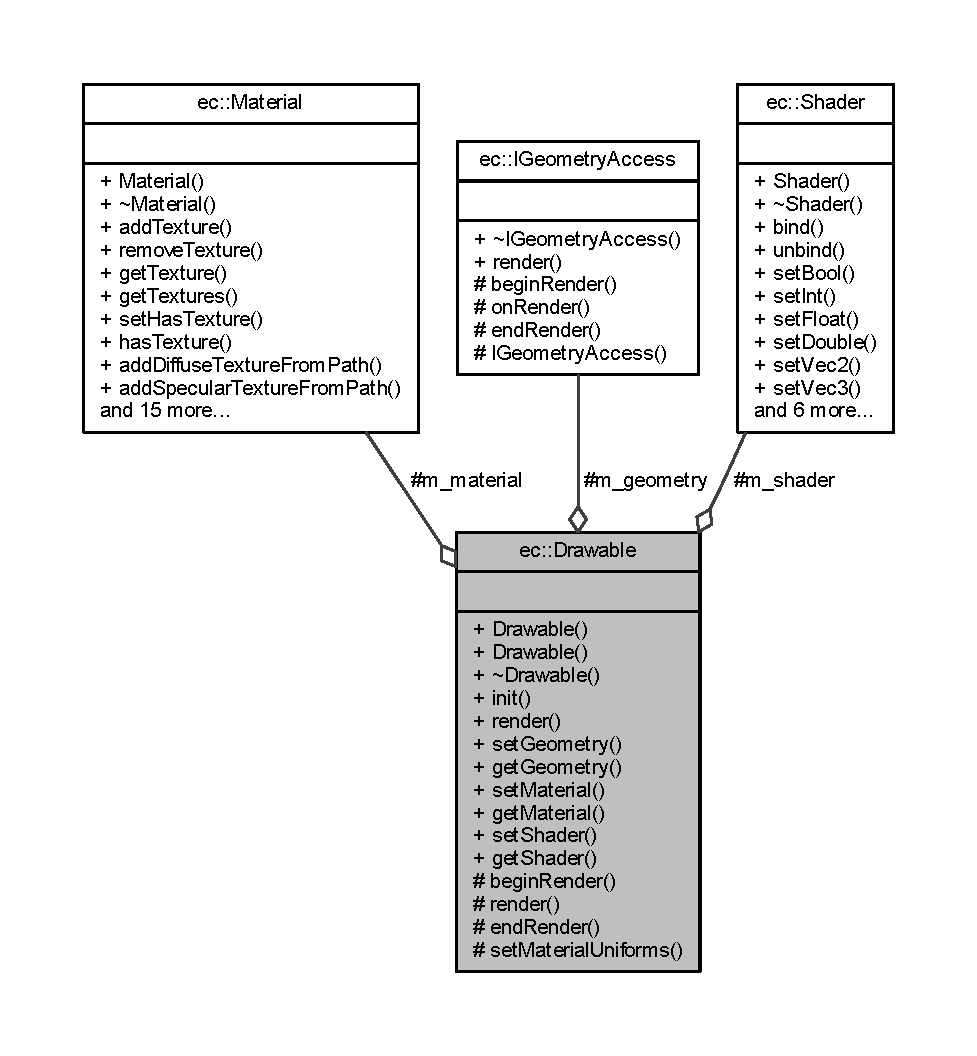
\includegraphics[height=550pt]{classec_1_1_drawable__coll__graph}
\end{center}
\end{figure}
\subsection*{Public Member Functions}
\begin{DoxyCompactItemize}
\item 
\mbox{\hyperlink{classec_1_1_drawable_adb3c4e7b4d3d510489a26b3d1a8094a2}{Drawable}} ()
\item 
\mbox{\hyperlink{classec_1_1_drawable_a1a6fee8a6543e001ee2943bda72e17cd}{Drawable}} (\mbox{\hyperlink{classec_1_1_i_geometry_access}{I\+Geometry\+Access}} $\ast$\mbox{\hyperlink{_resource_type_8h_af12fe3e5d8da3d7bd4c76e44cca2319c}{geometry}}, \mbox{\hyperlink{classec_1_1_material}{Material}} $\ast$\mbox{\hyperlink{_resource_type_8h_a16f6cac2c88eef38bdba4f004e042542}{material}}, \mbox{\hyperlink{classec_1_1_shader}{Shader}} $\ast$shader)
\begin{DoxyCompactList}\small\item\em \mbox{\hyperlink{classec_1_1_drawable}{Drawable}} constructor. \end{DoxyCompactList}\item 
virtual \mbox{\hyperlink{classec_1_1_drawable_a4a82e5cd6d6a47ad86ed42cfdda512d8}{$\sim$\+Drawable}} ()
\item 
void \mbox{\hyperlink{classec_1_1_drawable_ac494c72b1b0396dbe25a822da4e328a9}{init}} (\mbox{\hyperlink{classec_1_1_i_geometry_access}{I\+Geometry\+Access}} $\ast$\mbox{\hyperlink{_resource_type_8h_af12fe3e5d8da3d7bd4c76e44cca2319c}{geometry}}, \mbox{\hyperlink{classec_1_1_material}{Material}} $\ast$\mbox{\hyperlink{_resource_type_8h_a16f6cac2c88eef38bdba4f004e042542}{material}}, \mbox{\hyperlink{classec_1_1_shader}{Shader}} $\ast$shader)
\begin{DoxyCompactList}\small\item\em Initialize this drawable. Comfort function. \end{DoxyCompactList}\item 
virtual void \mbox{\hyperlink{classec_1_1_drawable_ac9d3345bd308fce8c99adbfc12c53106}{render}} (const glm\+::mat4 \&model)
\begin{DoxyCompactList}\small\item\em Render this drawable. \end{DoxyCompactList}\item 
void \mbox{\hyperlink{classec_1_1_drawable_a76bcb843ef5ced898724fa79a9b20250}{set\+Geometry}} (\mbox{\hyperlink{classec_1_1_i_geometry_access}{I\+Geometry\+Access}} $\ast$\mbox{\hyperlink{_resource_type_8h_af12fe3e5d8da3d7bd4c76e44cca2319c}{geometry}})
\begin{DoxyCompactList}\small\item\em Set the current geometry. \end{DoxyCompactList}\item 
\mbox{\hyperlink{classec_1_1_i_geometry_access}{I\+Geometry\+Access}} $\ast$ \mbox{\hyperlink{classec_1_1_drawable_a49a90aac40736ff3c182196c2b86c2f3}{get\+Geometry}} () const
\begin{DoxyCompactList}\small\item\em Get the current geometry. \end{DoxyCompactList}\item 
void \mbox{\hyperlink{classec_1_1_drawable_a0fc7868639a83830d4b60dfad85a0826}{set\+Material}} (\mbox{\hyperlink{classec_1_1_material}{Material}} $\ast$\mbox{\hyperlink{_resource_type_8h_a16f6cac2c88eef38bdba4f004e042542}{material}})
\begin{DoxyCompactList}\small\item\em Set the current material. \end{DoxyCompactList}\item 
\mbox{\hyperlink{classec_1_1_material}{Material}} $\ast$ \mbox{\hyperlink{classec_1_1_drawable_ac74210aca5428bedbf8af7abe9adbcc1}{get\+Material}} () const
\begin{DoxyCompactList}\small\item\em Get the current material. \end{DoxyCompactList}\item 
void \mbox{\hyperlink{classec_1_1_drawable_a413f373bb2cba109497377e18b084048}{set\+Shader}} (\mbox{\hyperlink{classec_1_1_shader}{Shader}} $\ast$shader)
\begin{DoxyCompactList}\small\item\em Set the current shader. \end{DoxyCompactList}\item 
\mbox{\hyperlink{classec_1_1_shader}{Shader}} $\ast$ \mbox{\hyperlink{classec_1_1_drawable_a7de4c8aa937bda1009c6428ceeb541c1}{get\+Shader}} () const
\begin{DoxyCompactList}\small\item\em Get the current shader. \end{DoxyCompactList}\end{DoxyCompactItemize}
\subsection*{Protected Member Functions}
\begin{DoxyCompactItemize}
\item 
virtual void \mbox{\hyperlink{classec_1_1_drawable_a9cb72c1eda19a82c849a291e7d45f2b8}{begin\+Render}} (const glm\+::mat4 \&model)
\begin{DoxyCompactList}\small\item\em Prepare drawable for rendering. \end{DoxyCompactList}\item 
virtual void \mbox{\hyperlink{classec_1_1_drawable_a7da17eae29c09e49d1a8c2c48e85f88a}{render}} ()
\begin{DoxyCompactList}\small\item\em Render the drawable. \end{DoxyCompactList}\item 
virtual void \mbox{\hyperlink{classec_1_1_drawable_abf99119cd72054a55d91a7605aa62e32}{end\+Render}} ()
\begin{DoxyCompactList}\small\item\em Finalize the rendering. \end{DoxyCompactList}\end{DoxyCompactItemize}
\subsection*{Static Protected Member Functions}
\begin{DoxyCompactItemize}
\item 
static void \mbox{\hyperlink{classec_1_1_drawable_af2b64f8e6faa71bee8cccb14387d8432}{set\+Material\+Uniforms}} (\mbox{\hyperlink{classec_1_1_shader}{Shader}} $\ast$shader, \mbox{\hyperlink{classec_1_1_material}{Material}} $\ast$\mbox{\hyperlink{_resource_type_8h_a16f6cac2c88eef38bdba4f004e042542}{material}})
\begin{DoxyCompactList}\small\item\em Transfer material data to the shader. \end{DoxyCompactList}\end{DoxyCompactItemize}
\subsection*{Protected Attributes}
\begin{DoxyCompactItemize}
\item 
\mbox{\hyperlink{classec_1_1_i_geometry_access}{I\+Geometry\+Access}} $\ast$ \mbox{\hyperlink{classec_1_1_drawable_a12fc649448250ab8a16e862495d22752}{m\+\_\+geometry}}
\item 
\mbox{\hyperlink{classec_1_1_material}{Material}} $\ast$ \mbox{\hyperlink{classec_1_1_drawable_ae95da71e937a2008a84300b8d29ac052}{m\+\_\+material}}
\item 
\mbox{\hyperlink{classec_1_1_shader}{Shader}} $\ast$ \mbox{\hyperlink{classec_1_1_drawable_aee71f07b65189391a7a465d880d744e3}{m\+\_\+shader}}
\end{DoxyCompactItemize}


\subsection{Detailed Description}
Core class for rendering geometry data with a certain material and shader. 

\subsection{Constructor \& Destructor Documentation}
\mbox{\Hypertarget{classec_1_1_drawable_adb3c4e7b4d3d510489a26b3d1a8094a2}\label{classec_1_1_drawable_adb3c4e7b4d3d510489a26b3d1a8094a2}} 
\index{ec\+::\+Drawable@{ec\+::\+Drawable}!Drawable@{Drawable}}
\index{Drawable@{Drawable}!ec\+::\+Drawable@{ec\+::\+Drawable}}
\subsubsection{\texorpdfstring{Drawable()}{Drawable()}\hspace{0.1cm}{\footnotesize\ttfamily [1/2]}}
{\footnotesize\ttfamily ec\+::\+Drawable\+::\+Drawable (\begin{DoxyParamCaption}{ }\end{DoxyParamCaption})\hspace{0.3cm}{\ttfamily [explicit]}}

\mbox{\Hypertarget{classec_1_1_drawable_a1a6fee8a6543e001ee2943bda72e17cd}\label{classec_1_1_drawable_a1a6fee8a6543e001ee2943bda72e17cd}} 
\index{ec\+::\+Drawable@{ec\+::\+Drawable}!Drawable@{Drawable}}
\index{Drawable@{Drawable}!ec\+::\+Drawable@{ec\+::\+Drawable}}
\subsubsection{\texorpdfstring{Drawable()}{Drawable()}\hspace{0.1cm}{\footnotesize\ttfamily [2/2]}}
{\footnotesize\ttfamily ec\+::\+Drawable\+::\+Drawable (\begin{DoxyParamCaption}\item[{\mbox{\hyperlink{classec_1_1_i_geometry_access}{I\+Geometry\+Access}} $\ast$}]{geometry,  }\item[{\mbox{\hyperlink{classec_1_1_material}{Material}} $\ast$}]{material,  }\item[{\mbox{\hyperlink{classec_1_1_shader}{Shader}} $\ast$}]{shader }\end{DoxyParamCaption})\hspace{0.3cm}{\ttfamily [explicit]}}



\mbox{\hyperlink{classec_1_1_drawable}{Drawable}} constructor. 


\begin{DoxyParams}{Parameters}
{\em geometry} & The geometry to render onto. \\
\hline
{\em material} & Color information. \\
\hline
{\em shader} & The shader used for drawing. \\
\hline
\end{DoxyParams}
\mbox{\Hypertarget{classec_1_1_drawable_a4a82e5cd6d6a47ad86ed42cfdda512d8}\label{classec_1_1_drawable_a4a82e5cd6d6a47ad86ed42cfdda512d8}} 
\index{ec\+::\+Drawable@{ec\+::\+Drawable}!````~Drawable@{$\sim$\+Drawable}}
\index{````~Drawable@{$\sim$\+Drawable}!ec\+::\+Drawable@{ec\+::\+Drawable}}
\subsubsection{\texorpdfstring{$\sim$\+Drawable()}{~Drawable()}}
{\footnotesize\ttfamily ec\+::\+Drawable\+::$\sim$\+Drawable (\begin{DoxyParamCaption}{ }\end{DoxyParamCaption})\hspace{0.3cm}{\ttfamily [virtual]}, {\ttfamily [default]}}



\subsection{Member Function Documentation}
\mbox{\Hypertarget{classec_1_1_drawable_a9cb72c1eda19a82c849a291e7d45f2b8}\label{classec_1_1_drawable_a9cb72c1eda19a82c849a291e7d45f2b8}} 
\index{ec\+::\+Drawable@{ec\+::\+Drawable}!begin\+Render@{begin\+Render}}
\index{begin\+Render@{begin\+Render}!ec\+::\+Drawable@{ec\+::\+Drawable}}
\subsubsection{\texorpdfstring{begin\+Render()}{beginRender()}}
{\footnotesize\ttfamily void ec\+::\+Drawable\+::begin\+Render (\begin{DoxyParamCaption}\item[{const glm\+::mat4 \&}]{model }\end{DoxyParamCaption})\hspace{0.3cm}{\ttfamily [protected]}, {\ttfamily [virtual]}}



Prepare drawable for rendering. 

\mbox{\Hypertarget{classec_1_1_drawable_abf99119cd72054a55d91a7605aa62e32}\label{classec_1_1_drawable_abf99119cd72054a55d91a7605aa62e32}} 
\index{ec\+::\+Drawable@{ec\+::\+Drawable}!end\+Render@{end\+Render}}
\index{end\+Render@{end\+Render}!ec\+::\+Drawable@{ec\+::\+Drawable}}
\subsubsection{\texorpdfstring{end\+Render()}{endRender()}}
{\footnotesize\ttfamily void ec\+::\+Drawable\+::end\+Render (\begin{DoxyParamCaption}{ }\end{DoxyParamCaption})\hspace{0.3cm}{\ttfamily [protected]}, {\ttfamily [virtual]}}



Finalize the rendering. 

\mbox{\Hypertarget{classec_1_1_drawable_a49a90aac40736ff3c182196c2b86c2f3}\label{classec_1_1_drawable_a49a90aac40736ff3c182196c2b86c2f3}} 
\index{ec\+::\+Drawable@{ec\+::\+Drawable}!get\+Geometry@{get\+Geometry}}
\index{get\+Geometry@{get\+Geometry}!ec\+::\+Drawable@{ec\+::\+Drawable}}
\subsubsection{\texorpdfstring{get\+Geometry()}{getGeometry()}}
{\footnotesize\ttfamily \mbox{\hyperlink{classec_1_1_i_geometry_access}{ec\+::\+I\+Geometry\+Access}} $\ast$ ec\+::\+Drawable\+::get\+Geometry (\begin{DoxyParamCaption}{ }\end{DoxyParamCaption}) const}



Get the current geometry. 

\mbox{\Hypertarget{classec_1_1_drawable_ac74210aca5428bedbf8af7abe9adbcc1}\label{classec_1_1_drawable_ac74210aca5428bedbf8af7abe9adbcc1}} 
\index{ec\+::\+Drawable@{ec\+::\+Drawable}!get\+Material@{get\+Material}}
\index{get\+Material@{get\+Material}!ec\+::\+Drawable@{ec\+::\+Drawable}}
\subsubsection{\texorpdfstring{get\+Material()}{getMaterial()}}
{\footnotesize\ttfamily \mbox{\hyperlink{classec_1_1_material}{ec\+::\+Material}} $\ast$ ec\+::\+Drawable\+::get\+Material (\begin{DoxyParamCaption}{ }\end{DoxyParamCaption}) const}



Get the current material. 

\mbox{\Hypertarget{classec_1_1_drawable_a7de4c8aa937bda1009c6428ceeb541c1}\label{classec_1_1_drawable_a7de4c8aa937bda1009c6428ceeb541c1}} 
\index{ec\+::\+Drawable@{ec\+::\+Drawable}!get\+Shader@{get\+Shader}}
\index{get\+Shader@{get\+Shader}!ec\+::\+Drawable@{ec\+::\+Drawable}}
\subsubsection{\texorpdfstring{get\+Shader()}{getShader()}}
{\footnotesize\ttfamily \mbox{\hyperlink{classec_1_1_shader}{ec\+::\+Shader}} $\ast$ ec\+::\+Drawable\+::get\+Shader (\begin{DoxyParamCaption}{ }\end{DoxyParamCaption}) const}



Get the current shader. 

\mbox{\Hypertarget{classec_1_1_drawable_ac494c72b1b0396dbe25a822da4e328a9}\label{classec_1_1_drawable_ac494c72b1b0396dbe25a822da4e328a9}} 
\index{ec\+::\+Drawable@{ec\+::\+Drawable}!init@{init}}
\index{init@{init}!ec\+::\+Drawable@{ec\+::\+Drawable}}
\subsubsection{\texorpdfstring{init()}{init()}}
{\footnotesize\ttfamily void ec\+::\+Drawable\+::init (\begin{DoxyParamCaption}\item[{\mbox{\hyperlink{classec_1_1_i_geometry_access}{I\+Geometry\+Access}} $\ast$}]{geometry,  }\item[{\mbox{\hyperlink{classec_1_1_material}{Material}} $\ast$}]{material,  }\item[{\mbox{\hyperlink{classec_1_1_shader}{Shader}} $\ast$}]{shader }\end{DoxyParamCaption})}



Initialize this drawable. Comfort function. 


\begin{DoxyParams}{Parameters}
{\em geometry} & The geometry to render onto. \\
\hline
{\em material} & Color information. \\
\hline
{\em shader} & The shader used for drawing. \\
\hline
\end{DoxyParams}
\mbox{\Hypertarget{classec_1_1_drawable_ac9d3345bd308fce8c99adbfc12c53106}\label{classec_1_1_drawable_ac9d3345bd308fce8c99adbfc12c53106}} 
\index{ec\+::\+Drawable@{ec\+::\+Drawable}!render@{render}}
\index{render@{render}!ec\+::\+Drawable@{ec\+::\+Drawable}}
\subsubsection{\texorpdfstring{render()}{render()}\hspace{0.1cm}{\footnotesize\ttfamily [1/2]}}
{\footnotesize\ttfamily void ec\+::\+Drawable\+::render (\begin{DoxyParamCaption}\item[{const glm\+::mat4 \&}]{model }\end{DoxyParamCaption})\hspace{0.3cm}{\ttfamily [virtual]}}



Render this drawable. 


\begin{DoxyParams}{Parameters}
{\em model} & Transformation of the object to draw. \\
\hline
\end{DoxyParams}
\mbox{\Hypertarget{classec_1_1_drawable_a7da17eae29c09e49d1a8c2c48e85f88a}\label{classec_1_1_drawable_a7da17eae29c09e49d1a8c2c48e85f88a}} 
\index{ec\+::\+Drawable@{ec\+::\+Drawable}!render@{render}}
\index{render@{render}!ec\+::\+Drawable@{ec\+::\+Drawable}}
\subsubsection{\texorpdfstring{render()}{render()}\hspace{0.1cm}{\footnotesize\ttfamily [2/2]}}
{\footnotesize\ttfamily void ec\+::\+Drawable\+::render (\begin{DoxyParamCaption}{ }\end{DoxyParamCaption})\hspace{0.3cm}{\ttfamily [protected]}, {\ttfamily [virtual]}}



Render the drawable. 

\mbox{\Hypertarget{classec_1_1_drawable_a76bcb843ef5ced898724fa79a9b20250}\label{classec_1_1_drawable_a76bcb843ef5ced898724fa79a9b20250}} 
\index{ec\+::\+Drawable@{ec\+::\+Drawable}!set\+Geometry@{set\+Geometry}}
\index{set\+Geometry@{set\+Geometry}!ec\+::\+Drawable@{ec\+::\+Drawable}}
\subsubsection{\texorpdfstring{set\+Geometry()}{setGeometry()}}
{\footnotesize\ttfamily void ec\+::\+Drawable\+::set\+Geometry (\begin{DoxyParamCaption}\item[{\mbox{\hyperlink{classec_1_1_i_geometry_access}{I\+Geometry\+Access}} $\ast$}]{geometry }\end{DoxyParamCaption})}



Set the current geometry. 

\mbox{\Hypertarget{classec_1_1_drawable_a0fc7868639a83830d4b60dfad85a0826}\label{classec_1_1_drawable_a0fc7868639a83830d4b60dfad85a0826}} 
\index{ec\+::\+Drawable@{ec\+::\+Drawable}!set\+Material@{set\+Material}}
\index{set\+Material@{set\+Material}!ec\+::\+Drawable@{ec\+::\+Drawable}}
\subsubsection{\texorpdfstring{set\+Material()}{setMaterial()}}
{\footnotesize\ttfamily void ec\+::\+Drawable\+::set\+Material (\begin{DoxyParamCaption}\item[{\mbox{\hyperlink{classec_1_1_material}{Material}} $\ast$}]{material }\end{DoxyParamCaption})}



Set the current material. 

\mbox{\Hypertarget{classec_1_1_drawable_af2b64f8e6faa71bee8cccb14387d8432}\label{classec_1_1_drawable_af2b64f8e6faa71bee8cccb14387d8432}} 
\index{ec\+::\+Drawable@{ec\+::\+Drawable}!set\+Material\+Uniforms@{set\+Material\+Uniforms}}
\index{set\+Material\+Uniforms@{set\+Material\+Uniforms}!ec\+::\+Drawable@{ec\+::\+Drawable}}
\subsubsection{\texorpdfstring{set\+Material\+Uniforms()}{setMaterialUniforms()}}
{\footnotesize\ttfamily void ec\+::\+Drawable\+::set\+Material\+Uniforms (\begin{DoxyParamCaption}\item[{\mbox{\hyperlink{classec_1_1_shader}{Shader}} $\ast$}]{shader,  }\item[{\mbox{\hyperlink{classec_1_1_material}{Material}} $\ast$}]{material }\end{DoxyParamCaption})\hspace{0.3cm}{\ttfamily [static]}, {\ttfamily [protected]}}



Transfer material data to the shader. 


\begin{DoxyParams}{Parameters}
{\em shader} & The shader to pass the data to. \\
\hline
{\em material} & The material data to pass. \\
\hline
\end{DoxyParams}
\mbox{\Hypertarget{classec_1_1_drawable_a413f373bb2cba109497377e18b084048}\label{classec_1_1_drawable_a413f373bb2cba109497377e18b084048}} 
\index{ec\+::\+Drawable@{ec\+::\+Drawable}!set\+Shader@{set\+Shader}}
\index{set\+Shader@{set\+Shader}!ec\+::\+Drawable@{ec\+::\+Drawable}}
\subsubsection{\texorpdfstring{set\+Shader()}{setShader()}}
{\footnotesize\ttfamily void ec\+::\+Drawable\+::set\+Shader (\begin{DoxyParamCaption}\item[{\mbox{\hyperlink{classec_1_1_shader}{Shader}} $\ast$}]{shader }\end{DoxyParamCaption})}



Set the current shader. 



\subsection{Member Data Documentation}
\mbox{\Hypertarget{classec_1_1_drawable_a12fc649448250ab8a16e862495d22752}\label{classec_1_1_drawable_a12fc649448250ab8a16e862495d22752}} 
\index{ec\+::\+Drawable@{ec\+::\+Drawable}!m\+\_\+geometry@{m\+\_\+geometry}}
\index{m\+\_\+geometry@{m\+\_\+geometry}!ec\+::\+Drawable@{ec\+::\+Drawable}}
\subsubsection{\texorpdfstring{m\+\_\+geometry}{m\_geometry}}
{\footnotesize\ttfamily \mbox{\hyperlink{classec_1_1_i_geometry_access}{I\+Geometry\+Access}}$\ast$ ec\+::\+Drawable\+::m\+\_\+geometry\hspace{0.3cm}{\ttfamily [protected]}}

\mbox{\Hypertarget{classec_1_1_drawable_ae95da71e937a2008a84300b8d29ac052}\label{classec_1_1_drawable_ae95da71e937a2008a84300b8d29ac052}} 
\index{ec\+::\+Drawable@{ec\+::\+Drawable}!m\+\_\+material@{m\+\_\+material}}
\index{m\+\_\+material@{m\+\_\+material}!ec\+::\+Drawable@{ec\+::\+Drawable}}
\subsubsection{\texorpdfstring{m\+\_\+material}{m\_material}}
{\footnotesize\ttfamily \mbox{\hyperlink{classec_1_1_material}{Material}}$\ast$ ec\+::\+Drawable\+::m\+\_\+material\hspace{0.3cm}{\ttfamily [protected]}}

\mbox{\Hypertarget{classec_1_1_drawable_aee71f07b65189391a7a465d880d744e3}\label{classec_1_1_drawable_aee71f07b65189391a7a465d880d744e3}} 
\index{ec\+::\+Drawable@{ec\+::\+Drawable}!m\+\_\+shader@{m\+\_\+shader}}
\index{m\+\_\+shader@{m\+\_\+shader}!ec\+::\+Drawable@{ec\+::\+Drawable}}
\subsubsection{\texorpdfstring{m\+\_\+shader}{m\_shader}}
{\footnotesize\ttfamily \mbox{\hyperlink{classec_1_1_shader}{Shader}}$\ast$ ec\+::\+Drawable\+::m\+\_\+shader\hspace{0.3cm}{\ttfamily [protected]}}



The documentation for this class was generated from the following files\+:\begin{DoxyCompactItemize}
\item 
C\+:/\+Library/\+Job/\+Projekte/\+Simulation\+Visualization/\+Eye\+Candy3\+D/\+Eye\+Candy3\+D/include/\+E\+C3\+D/\+Core/\mbox{\hyperlink{_drawable_8h}{Drawable.\+h}}\item 
C\+:/\+Library/\+Job/\+Projekte/\+Simulation\+Visualization/\+Eye\+Candy3\+D/\+Eye\+Candy3\+D/src/\+Core/\mbox{\hyperlink{_drawable_8cpp}{Drawable.\+cpp}}\end{DoxyCompactItemize}

\hypertarget{structec_1_1_drop_event}{}\section{ec\+:\+:Drop\+Event Struct Reference}
\label{structec_1_1_drop_event}\index{ec\+::\+Drop\+Event@{ec\+::\+Drop\+Event}}


An event generated by dragging and dropping links into a window.  




{\ttfamily \#include $<$Input\+Event.\+h$>$}



Collaboration diagram for ec\+:\+:Drop\+Event\+:\nopagebreak
\begin{figure}[H]
\begin{center}
\leavevmode
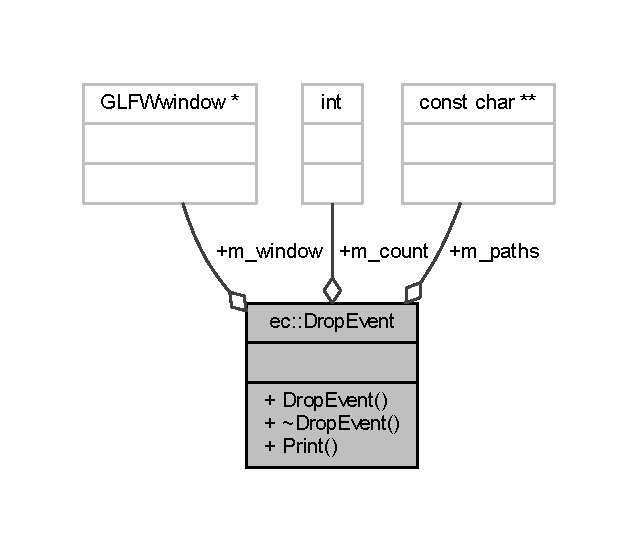
\includegraphics[width=305pt]{structec_1_1_drop_event__coll__graph}
\end{center}
\end{figure}
\subsection*{Public Member Functions}
\begin{DoxyCompactItemize}
\item 
\mbox{\hyperlink{structec_1_1_drop_event_a6ae6f5be022c3809bc204c365dc11cbc}{Drop\+Event}} ()
\item 
\mbox{\hyperlink{structec_1_1_drop_event_a955d74612461f4100890101ddd1c2528}{Drop\+Event}} (int x, int y, G\+L\+F\+Wwindow $\ast$window, int \mbox{\hyperlink{namespaceec_a30e2a743ebdeb02ac68a6cfa50f629c7ae2942a04780e223b215eb8b663cf5353}{count}}, const char $\ast$$\ast$paths)
\item 
\mbox{\hyperlink{structec_1_1_drop_event_ad68bca5b7ca0c65690fc85d682d057db}{$\sim$\+Drop\+Event}} ()
\item 
void \mbox{\hyperlink{structec_1_1_drop_event_a6cda7eaf944e0b94f49a8523c7da2656}{print}} () const
\end{DoxyCompactItemize}
\subsection*{Public Attributes}
\begin{DoxyCompactItemize}
\item 
G\+L\+F\+Wwindow $\ast$ \mbox{\hyperlink{structec_1_1_drop_event_a526c7694184ab65111ca5f8f4f2384fa}{m\+\_\+window}}
\item 
int \mbox{\hyperlink{structec_1_1_drop_event_ae1b8807808b78aecbdb27d51a4ab87eb}{m\+\_\+x}}
\item 
int \mbox{\hyperlink{structec_1_1_drop_event_a59338dd4b8cd47b7f025908a63be2e92}{m\+\_\+y}}
\item 
int \mbox{\hyperlink{structec_1_1_drop_event_a63c1174cdefa0a30b15667c9fa070a41}{m\+\_\+count}}
\item 
const char $\ast$$\ast$ \mbox{\hyperlink{structec_1_1_drop_event_ad7bdb28144cd5ccb2c13c4dbacff40cb}{m\+\_\+paths}}
\end{DoxyCompactItemize}


\subsection{Detailed Description}
An event generated by dragging and dropping links into a window. 

\subsection{Constructor \& Destructor Documentation}
\mbox{\Hypertarget{structec_1_1_drop_event_a6ae6f5be022c3809bc204c365dc11cbc}\label{structec_1_1_drop_event_a6ae6f5be022c3809bc204c365dc11cbc}} 
\index{ec\+::\+Drop\+Event@{ec\+::\+Drop\+Event}!Drop\+Event@{Drop\+Event}}
\index{Drop\+Event@{Drop\+Event}!ec\+::\+Drop\+Event@{ec\+::\+Drop\+Event}}
\subsubsection{\texorpdfstring{Drop\+Event()}{DropEvent()}\hspace{0.1cm}{\footnotesize\ttfamily [1/2]}}
{\footnotesize\ttfamily ec\+::\+Drop\+Event\+::\+Drop\+Event (\begin{DoxyParamCaption}{ }\end{DoxyParamCaption})\hspace{0.3cm}{\ttfamily [explicit]}}

\mbox{\Hypertarget{structec_1_1_drop_event_a955d74612461f4100890101ddd1c2528}\label{structec_1_1_drop_event_a955d74612461f4100890101ddd1c2528}} 
\index{ec\+::\+Drop\+Event@{ec\+::\+Drop\+Event}!Drop\+Event@{Drop\+Event}}
\index{Drop\+Event@{Drop\+Event}!ec\+::\+Drop\+Event@{ec\+::\+Drop\+Event}}
\subsubsection{\texorpdfstring{Drop\+Event()}{DropEvent()}\hspace{0.1cm}{\footnotesize\ttfamily [2/2]}}
{\footnotesize\ttfamily ec\+::\+Drop\+Event\+::\+Drop\+Event (\begin{DoxyParamCaption}\item[{int}]{x,  }\item[{int}]{y,  }\item[{G\+L\+F\+Wwindow $\ast$}]{window,  }\item[{int}]{count,  }\item[{const char $\ast$$\ast$}]{paths }\end{DoxyParamCaption})\hspace{0.3cm}{\ttfamily [explicit]}}

\mbox{\Hypertarget{structec_1_1_drop_event_ad68bca5b7ca0c65690fc85d682d057db}\label{structec_1_1_drop_event_ad68bca5b7ca0c65690fc85d682d057db}} 
\index{ec\+::\+Drop\+Event@{ec\+::\+Drop\+Event}!````~Drop\+Event@{$\sim$\+Drop\+Event}}
\index{````~Drop\+Event@{$\sim$\+Drop\+Event}!ec\+::\+Drop\+Event@{ec\+::\+Drop\+Event}}
\subsubsection{\texorpdfstring{$\sim$\+Drop\+Event()}{~DropEvent()}}
{\footnotesize\ttfamily ec\+::\+Drop\+Event\+::$\sim$\+Drop\+Event (\begin{DoxyParamCaption}{ }\end{DoxyParamCaption})\hspace{0.3cm}{\ttfamily [default]}}



\subsection{Member Function Documentation}
\mbox{\Hypertarget{structec_1_1_drop_event_a6cda7eaf944e0b94f49a8523c7da2656}\label{structec_1_1_drop_event_a6cda7eaf944e0b94f49a8523c7da2656}} 
\index{ec\+::\+Drop\+Event@{ec\+::\+Drop\+Event}!print@{print}}
\index{print@{print}!ec\+::\+Drop\+Event@{ec\+::\+Drop\+Event}}
\subsubsection{\texorpdfstring{print()}{print()}}
{\footnotesize\ttfamily void ec\+::\+Drop\+Event\+::print (\begin{DoxyParamCaption}{ }\end{DoxyParamCaption}) const}



\subsection{Member Data Documentation}
\mbox{\Hypertarget{structec_1_1_drop_event_a63c1174cdefa0a30b15667c9fa070a41}\label{structec_1_1_drop_event_a63c1174cdefa0a30b15667c9fa070a41}} 
\index{ec\+::\+Drop\+Event@{ec\+::\+Drop\+Event}!m\+\_\+count@{m\+\_\+count}}
\index{m\+\_\+count@{m\+\_\+count}!ec\+::\+Drop\+Event@{ec\+::\+Drop\+Event}}
\subsubsection{\texorpdfstring{m\+\_\+count}{m\_count}}
{\footnotesize\ttfamily int ec\+::\+Drop\+Event\+::m\+\_\+count}

\mbox{\Hypertarget{structec_1_1_drop_event_ad7bdb28144cd5ccb2c13c4dbacff40cb}\label{structec_1_1_drop_event_ad7bdb28144cd5ccb2c13c4dbacff40cb}} 
\index{ec\+::\+Drop\+Event@{ec\+::\+Drop\+Event}!m\+\_\+paths@{m\+\_\+paths}}
\index{m\+\_\+paths@{m\+\_\+paths}!ec\+::\+Drop\+Event@{ec\+::\+Drop\+Event}}
\subsubsection{\texorpdfstring{m\+\_\+paths}{m\_paths}}
{\footnotesize\ttfamily const char$\ast$$\ast$ ec\+::\+Drop\+Event\+::m\+\_\+paths}

\mbox{\Hypertarget{structec_1_1_drop_event_a526c7694184ab65111ca5f8f4f2384fa}\label{structec_1_1_drop_event_a526c7694184ab65111ca5f8f4f2384fa}} 
\index{ec\+::\+Drop\+Event@{ec\+::\+Drop\+Event}!m\+\_\+window@{m\+\_\+window}}
\index{m\+\_\+window@{m\+\_\+window}!ec\+::\+Drop\+Event@{ec\+::\+Drop\+Event}}
\subsubsection{\texorpdfstring{m\+\_\+window}{m\_window}}
{\footnotesize\ttfamily G\+L\+F\+Wwindow$\ast$ ec\+::\+Drop\+Event\+::m\+\_\+window}

\mbox{\Hypertarget{structec_1_1_drop_event_ae1b8807808b78aecbdb27d51a4ab87eb}\label{structec_1_1_drop_event_ae1b8807808b78aecbdb27d51a4ab87eb}} 
\index{ec\+::\+Drop\+Event@{ec\+::\+Drop\+Event}!m\+\_\+x@{m\+\_\+x}}
\index{m\+\_\+x@{m\+\_\+x}!ec\+::\+Drop\+Event@{ec\+::\+Drop\+Event}}
\subsubsection{\texorpdfstring{m\+\_\+x}{m\_x}}
{\footnotesize\ttfamily int ec\+::\+Drop\+Event\+::m\+\_\+x}

\mbox{\Hypertarget{structec_1_1_drop_event_a59338dd4b8cd47b7f025908a63be2e92}\label{structec_1_1_drop_event_a59338dd4b8cd47b7f025908a63be2e92}} 
\index{ec\+::\+Drop\+Event@{ec\+::\+Drop\+Event}!m\+\_\+y@{m\+\_\+y}}
\index{m\+\_\+y@{m\+\_\+y}!ec\+::\+Drop\+Event@{ec\+::\+Drop\+Event}}
\subsubsection{\texorpdfstring{m\+\_\+y}{m\_y}}
{\footnotesize\ttfamily int ec\+::\+Drop\+Event\+::m\+\_\+y}



The documentation for this struct was generated from the following files\+:\begin{DoxyCompactItemize}
\item 
C\+:/\+Library/\+Job/\+Projekte/\+Simulation\+Visualization/\+Eye\+Candy3\+D/\+Eye\+Candy3\+D/include/\+E\+C3\+D/\+Core/\mbox{\hyperlink{_input_event_8h}{Input\+Event.\+h}}\item 
C\+:/\+Library/\+Job/\+Projekte/\+Simulation\+Visualization/\+Eye\+Candy3\+D/\+Eye\+Candy3\+D/src/\+Core/\mbox{\hyperlink{_input_event_8cpp}{Input\+Event.\+cpp}}\end{DoxyCompactItemize}

\hypertarget{unionec_1_1_input_event_1_1_event_data}{}\section{ec\+:\+:Input\+Event\+:\+:Event\+Data Union Reference}
\label{unionec_1_1_input_event_1_1_event_data}\index{ec\+::\+Input\+Event\+::\+Event\+Data@{ec\+::\+Input\+Event\+::\+Event\+Data}}


{\ttfamily \#include $<$Input\+Event.\+h$>$}



Collaboration diagram for ec\+:\+:Input\+Event\+:\+:Event\+Data\+:\nopagebreak
\begin{figure}[H]
\begin{center}
\leavevmode
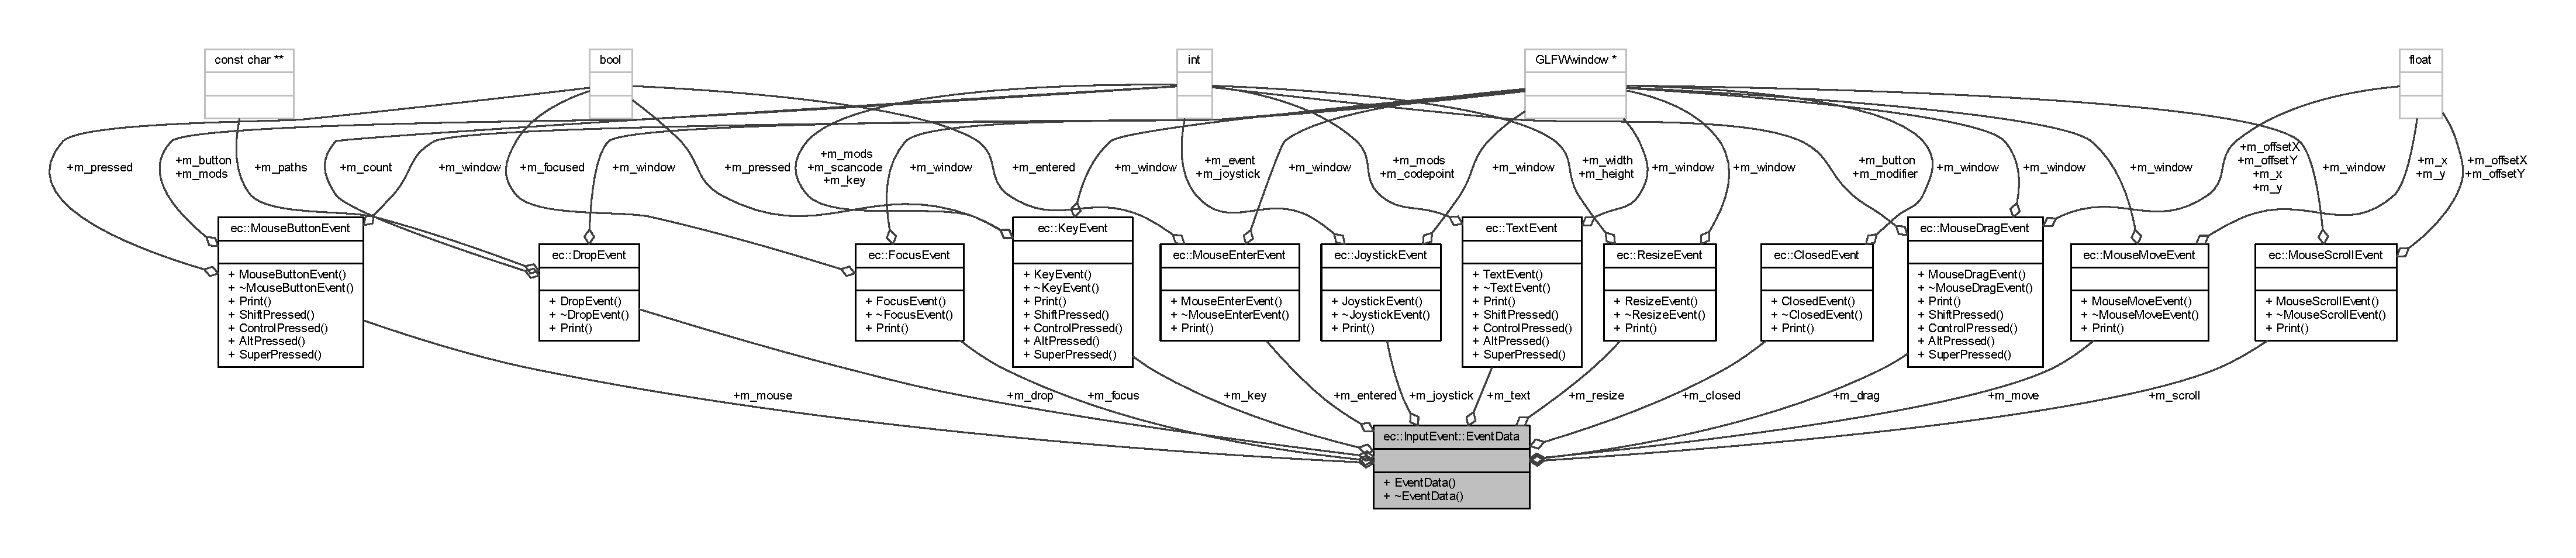
\includegraphics[width=350pt]{unionec_1_1_input_event_1_1_event_data__coll__graph}
\end{center}
\end{figure}
\subsection*{Public Member Functions}
\begin{DoxyCompactItemize}
\item 
\mbox{\hyperlink{unionec_1_1_input_event_1_1_event_data_a07feefe51335e0521a10f2032d5a7dbc}{Event\+Data}} ()
\item 
\mbox{\hyperlink{unionec_1_1_input_event_1_1_event_data_aa5609c794c2f689ecea99efa7c1a16b0}{$\sim$\+Event\+Data}} ()
\end{DoxyCompactItemize}
\subsection*{Public Attributes}
\begin{DoxyCompactItemize}
\item 
\mbox{\hyperlink{structec_1_1_mouse_move_event}{Mouse\+Move\+Event}} \mbox{\hyperlink{unionec_1_1_input_event_1_1_event_data_a0592d7314321622bf817ac5ac8cf937c}{m\+\_\+move}}
\item 
\mbox{\hyperlink{structec_1_1_mouse_drag_event}{Mouse\+Drag\+Event}} \mbox{\hyperlink{unionec_1_1_input_event_1_1_event_data_a91a200655ac87b3d464a06d7d192bea4}{m\+\_\+drag}}
\item 
\mbox{\hyperlink{structec_1_1_mouse_scroll_event}{Mouse\+Scroll\+Event}} \mbox{\hyperlink{unionec_1_1_input_event_1_1_event_data_a7cb5c60064ca006bcf29d8594472ce10}{m\+\_\+scroll}}
\item 
\mbox{\hyperlink{structec_1_1_mouse_enter_event}{Mouse\+Enter\+Event}} \mbox{\hyperlink{unionec_1_1_input_event_1_1_event_data_ae53bd6defd14eb18ab294f01ab5632b1}{m\+\_\+entered}}
\item 
\mbox{\hyperlink{structec_1_1_mouse_button_event}{Mouse\+Button\+Event}} \mbox{\hyperlink{unionec_1_1_input_event_1_1_event_data_a944e5e6d14fe8eb20f39d10def46d3f8}{m\+\_\+mouse}}
\item 
\mbox{\hyperlink{structec_1_1_joystick_event}{Joystick\+Event}} \mbox{\hyperlink{unionec_1_1_input_event_1_1_event_data_a3df014ee916cae08c2c43da4a935642f}{m\+\_\+joystick}}
\item 
\mbox{\hyperlink{structec_1_1_key_event}{Key\+Event}} \mbox{\hyperlink{unionec_1_1_input_event_1_1_event_data_ac173ac49d3a99ca0dfeab8adc6860dbc}{m\+\_\+key}}
\item 
\mbox{\hyperlink{structec_1_1_text_event}{Text\+Event}} \mbox{\hyperlink{unionec_1_1_input_event_1_1_event_data_acd584a87f8886a1df789e075949f8f54}{m\+\_\+text}}
\item 
\mbox{\hyperlink{structec_1_1_drop_event}{Drop\+Event}} \mbox{\hyperlink{unionec_1_1_input_event_1_1_event_data_a9e9c97bd137c4efc47741b0671c22da0}{m\+\_\+drop}}
\item 
\mbox{\hyperlink{structec_1_1_resize_event}{Resize\+Event}} \mbox{\hyperlink{unionec_1_1_input_event_1_1_event_data_aa4baeac14bdea798dbe97b0482cd2845}{m\+\_\+resize}}
\item 
\mbox{\hyperlink{structec_1_1_focus_event}{Focus\+Event}} \mbox{\hyperlink{unionec_1_1_input_event_1_1_event_data_a1533b88d1ec3fe02b2dc20188e3b15d3}{m\+\_\+focus}}
\item 
\mbox{\hyperlink{structec_1_1_closed_event}{Closed\+Event}} \mbox{\hyperlink{unionec_1_1_input_event_1_1_event_data_a6efd3bf979fade6572afd1943b192fbf}{m\+\_\+closed}}
\end{DoxyCompactItemize}


\subsection{Constructor \& Destructor Documentation}
\mbox{\Hypertarget{unionec_1_1_input_event_1_1_event_data_a07feefe51335e0521a10f2032d5a7dbc}\label{unionec_1_1_input_event_1_1_event_data_a07feefe51335e0521a10f2032d5a7dbc}} 
\index{ec\+::\+Input\+Event\+::\+Event\+Data@{ec\+::\+Input\+Event\+::\+Event\+Data}!Event\+Data@{Event\+Data}}
\index{Event\+Data@{Event\+Data}!ec\+::\+Input\+Event\+::\+Event\+Data@{ec\+::\+Input\+Event\+::\+Event\+Data}}
\subsubsection{\texorpdfstring{Event\+Data()}{EventData()}}
{\footnotesize\ttfamily ec\+::\+Input\+Event\+::\+Event\+Data\+::\+Event\+Data (\begin{DoxyParamCaption}{ }\end{DoxyParamCaption})\hspace{0.3cm}{\ttfamily [inline]}}

\mbox{\Hypertarget{unionec_1_1_input_event_1_1_event_data_aa5609c794c2f689ecea99efa7c1a16b0}\label{unionec_1_1_input_event_1_1_event_data_aa5609c794c2f689ecea99efa7c1a16b0}} 
\index{ec\+::\+Input\+Event\+::\+Event\+Data@{ec\+::\+Input\+Event\+::\+Event\+Data}!````~Event\+Data@{$\sim$\+Event\+Data}}
\index{````~Event\+Data@{$\sim$\+Event\+Data}!ec\+::\+Input\+Event\+::\+Event\+Data@{ec\+::\+Input\+Event\+::\+Event\+Data}}
\subsubsection{\texorpdfstring{$\sim$\+Event\+Data()}{~EventData()}}
{\footnotesize\ttfamily ec\+::\+Input\+Event\+::\+Event\+Data\+::$\sim$\+Event\+Data (\begin{DoxyParamCaption}{ }\end{DoxyParamCaption})\hspace{0.3cm}{\ttfamily [inline]}}



\subsection{Member Data Documentation}
\mbox{\Hypertarget{unionec_1_1_input_event_1_1_event_data_a6efd3bf979fade6572afd1943b192fbf}\label{unionec_1_1_input_event_1_1_event_data_a6efd3bf979fade6572afd1943b192fbf}} 
\index{ec\+::\+Input\+Event\+::\+Event\+Data@{ec\+::\+Input\+Event\+::\+Event\+Data}!m\+\_\+closed@{m\+\_\+closed}}
\index{m\+\_\+closed@{m\+\_\+closed}!ec\+::\+Input\+Event\+::\+Event\+Data@{ec\+::\+Input\+Event\+::\+Event\+Data}}
\subsubsection{\texorpdfstring{m\+\_\+closed}{m\_closed}}
{\footnotesize\ttfamily \mbox{\hyperlink{structec_1_1_closed_event}{Closed\+Event}} ec\+::\+Input\+Event\+::\+Event\+Data\+::m\+\_\+closed}

\mbox{\Hypertarget{unionec_1_1_input_event_1_1_event_data_a91a200655ac87b3d464a06d7d192bea4}\label{unionec_1_1_input_event_1_1_event_data_a91a200655ac87b3d464a06d7d192bea4}} 
\index{ec\+::\+Input\+Event\+::\+Event\+Data@{ec\+::\+Input\+Event\+::\+Event\+Data}!m\+\_\+drag@{m\+\_\+drag}}
\index{m\+\_\+drag@{m\+\_\+drag}!ec\+::\+Input\+Event\+::\+Event\+Data@{ec\+::\+Input\+Event\+::\+Event\+Data}}
\subsubsection{\texorpdfstring{m\+\_\+drag}{m\_drag}}
{\footnotesize\ttfamily \mbox{\hyperlink{structec_1_1_mouse_drag_event}{Mouse\+Drag\+Event}} ec\+::\+Input\+Event\+::\+Event\+Data\+::m\+\_\+drag}

\mbox{\Hypertarget{unionec_1_1_input_event_1_1_event_data_a9e9c97bd137c4efc47741b0671c22da0}\label{unionec_1_1_input_event_1_1_event_data_a9e9c97bd137c4efc47741b0671c22da0}} 
\index{ec\+::\+Input\+Event\+::\+Event\+Data@{ec\+::\+Input\+Event\+::\+Event\+Data}!m\+\_\+drop@{m\+\_\+drop}}
\index{m\+\_\+drop@{m\+\_\+drop}!ec\+::\+Input\+Event\+::\+Event\+Data@{ec\+::\+Input\+Event\+::\+Event\+Data}}
\subsubsection{\texorpdfstring{m\+\_\+drop}{m\_drop}}
{\footnotesize\ttfamily \mbox{\hyperlink{structec_1_1_drop_event}{Drop\+Event}} ec\+::\+Input\+Event\+::\+Event\+Data\+::m\+\_\+drop}

\mbox{\Hypertarget{unionec_1_1_input_event_1_1_event_data_ae53bd6defd14eb18ab294f01ab5632b1}\label{unionec_1_1_input_event_1_1_event_data_ae53bd6defd14eb18ab294f01ab5632b1}} 
\index{ec\+::\+Input\+Event\+::\+Event\+Data@{ec\+::\+Input\+Event\+::\+Event\+Data}!m\+\_\+entered@{m\+\_\+entered}}
\index{m\+\_\+entered@{m\+\_\+entered}!ec\+::\+Input\+Event\+::\+Event\+Data@{ec\+::\+Input\+Event\+::\+Event\+Data}}
\subsubsection{\texorpdfstring{m\+\_\+entered}{m\_entered}}
{\footnotesize\ttfamily \mbox{\hyperlink{structec_1_1_mouse_enter_event}{Mouse\+Enter\+Event}} ec\+::\+Input\+Event\+::\+Event\+Data\+::m\+\_\+entered}

\mbox{\Hypertarget{unionec_1_1_input_event_1_1_event_data_a1533b88d1ec3fe02b2dc20188e3b15d3}\label{unionec_1_1_input_event_1_1_event_data_a1533b88d1ec3fe02b2dc20188e3b15d3}} 
\index{ec\+::\+Input\+Event\+::\+Event\+Data@{ec\+::\+Input\+Event\+::\+Event\+Data}!m\+\_\+focus@{m\+\_\+focus}}
\index{m\+\_\+focus@{m\+\_\+focus}!ec\+::\+Input\+Event\+::\+Event\+Data@{ec\+::\+Input\+Event\+::\+Event\+Data}}
\subsubsection{\texorpdfstring{m\+\_\+focus}{m\_focus}}
{\footnotesize\ttfamily \mbox{\hyperlink{structec_1_1_focus_event}{Focus\+Event}} ec\+::\+Input\+Event\+::\+Event\+Data\+::m\+\_\+focus}

\mbox{\Hypertarget{unionec_1_1_input_event_1_1_event_data_a3df014ee916cae08c2c43da4a935642f}\label{unionec_1_1_input_event_1_1_event_data_a3df014ee916cae08c2c43da4a935642f}} 
\index{ec\+::\+Input\+Event\+::\+Event\+Data@{ec\+::\+Input\+Event\+::\+Event\+Data}!m\+\_\+joystick@{m\+\_\+joystick}}
\index{m\+\_\+joystick@{m\+\_\+joystick}!ec\+::\+Input\+Event\+::\+Event\+Data@{ec\+::\+Input\+Event\+::\+Event\+Data}}
\subsubsection{\texorpdfstring{m\+\_\+joystick}{m\_joystick}}
{\footnotesize\ttfamily \mbox{\hyperlink{structec_1_1_joystick_event}{Joystick\+Event}} ec\+::\+Input\+Event\+::\+Event\+Data\+::m\+\_\+joystick}

\mbox{\Hypertarget{unionec_1_1_input_event_1_1_event_data_ac173ac49d3a99ca0dfeab8adc6860dbc}\label{unionec_1_1_input_event_1_1_event_data_ac173ac49d3a99ca0dfeab8adc6860dbc}} 
\index{ec\+::\+Input\+Event\+::\+Event\+Data@{ec\+::\+Input\+Event\+::\+Event\+Data}!m\+\_\+key@{m\+\_\+key}}
\index{m\+\_\+key@{m\+\_\+key}!ec\+::\+Input\+Event\+::\+Event\+Data@{ec\+::\+Input\+Event\+::\+Event\+Data}}
\subsubsection{\texorpdfstring{m\+\_\+key}{m\_key}}
{\footnotesize\ttfamily \mbox{\hyperlink{structec_1_1_key_event}{Key\+Event}} ec\+::\+Input\+Event\+::\+Event\+Data\+::m\+\_\+key}

\mbox{\Hypertarget{unionec_1_1_input_event_1_1_event_data_a944e5e6d14fe8eb20f39d10def46d3f8}\label{unionec_1_1_input_event_1_1_event_data_a944e5e6d14fe8eb20f39d10def46d3f8}} 
\index{ec\+::\+Input\+Event\+::\+Event\+Data@{ec\+::\+Input\+Event\+::\+Event\+Data}!m\+\_\+mouse@{m\+\_\+mouse}}
\index{m\+\_\+mouse@{m\+\_\+mouse}!ec\+::\+Input\+Event\+::\+Event\+Data@{ec\+::\+Input\+Event\+::\+Event\+Data}}
\subsubsection{\texorpdfstring{m\+\_\+mouse}{m\_mouse}}
{\footnotesize\ttfamily \mbox{\hyperlink{structec_1_1_mouse_button_event}{Mouse\+Button\+Event}} ec\+::\+Input\+Event\+::\+Event\+Data\+::m\+\_\+mouse}

\mbox{\Hypertarget{unionec_1_1_input_event_1_1_event_data_a0592d7314321622bf817ac5ac8cf937c}\label{unionec_1_1_input_event_1_1_event_data_a0592d7314321622bf817ac5ac8cf937c}} 
\index{ec\+::\+Input\+Event\+::\+Event\+Data@{ec\+::\+Input\+Event\+::\+Event\+Data}!m\+\_\+move@{m\+\_\+move}}
\index{m\+\_\+move@{m\+\_\+move}!ec\+::\+Input\+Event\+::\+Event\+Data@{ec\+::\+Input\+Event\+::\+Event\+Data}}
\subsubsection{\texorpdfstring{m\+\_\+move}{m\_move}}
{\footnotesize\ttfamily \mbox{\hyperlink{structec_1_1_mouse_move_event}{Mouse\+Move\+Event}} ec\+::\+Input\+Event\+::\+Event\+Data\+::m\+\_\+move}

\mbox{\Hypertarget{unionec_1_1_input_event_1_1_event_data_aa4baeac14bdea798dbe97b0482cd2845}\label{unionec_1_1_input_event_1_1_event_data_aa4baeac14bdea798dbe97b0482cd2845}} 
\index{ec\+::\+Input\+Event\+::\+Event\+Data@{ec\+::\+Input\+Event\+::\+Event\+Data}!m\+\_\+resize@{m\+\_\+resize}}
\index{m\+\_\+resize@{m\+\_\+resize}!ec\+::\+Input\+Event\+::\+Event\+Data@{ec\+::\+Input\+Event\+::\+Event\+Data}}
\subsubsection{\texorpdfstring{m\+\_\+resize}{m\_resize}}
{\footnotesize\ttfamily \mbox{\hyperlink{structec_1_1_resize_event}{Resize\+Event}} ec\+::\+Input\+Event\+::\+Event\+Data\+::m\+\_\+resize}

\mbox{\Hypertarget{unionec_1_1_input_event_1_1_event_data_a7cb5c60064ca006bcf29d8594472ce10}\label{unionec_1_1_input_event_1_1_event_data_a7cb5c60064ca006bcf29d8594472ce10}} 
\index{ec\+::\+Input\+Event\+::\+Event\+Data@{ec\+::\+Input\+Event\+::\+Event\+Data}!m\+\_\+scroll@{m\+\_\+scroll}}
\index{m\+\_\+scroll@{m\+\_\+scroll}!ec\+::\+Input\+Event\+::\+Event\+Data@{ec\+::\+Input\+Event\+::\+Event\+Data}}
\subsubsection{\texorpdfstring{m\+\_\+scroll}{m\_scroll}}
{\footnotesize\ttfamily \mbox{\hyperlink{structec_1_1_mouse_scroll_event}{Mouse\+Scroll\+Event}} ec\+::\+Input\+Event\+::\+Event\+Data\+::m\+\_\+scroll}

\mbox{\Hypertarget{unionec_1_1_input_event_1_1_event_data_acd584a87f8886a1df789e075949f8f54}\label{unionec_1_1_input_event_1_1_event_data_acd584a87f8886a1df789e075949f8f54}} 
\index{ec\+::\+Input\+Event\+::\+Event\+Data@{ec\+::\+Input\+Event\+::\+Event\+Data}!m\+\_\+text@{m\+\_\+text}}
\index{m\+\_\+text@{m\+\_\+text}!ec\+::\+Input\+Event\+::\+Event\+Data@{ec\+::\+Input\+Event\+::\+Event\+Data}}
\subsubsection{\texorpdfstring{m\+\_\+text}{m\_text}}
{\footnotesize\ttfamily \mbox{\hyperlink{structec_1_1_text_event}{Text\+Event}} ec\+::\+Input\+Event\+::\+Event\+Data\+::m\+\_\+text}



The documentation for this union was generated from the following file\+:\begin{DoxyCompactItemize}
\item 
D\+:/\+Library/\+Documents/\+Job/\+Forschungsmaster/\+Projekte/\+Eye\+Candy3\+D/\+Eye\+Candy3\+D/include/\+E\+C3\+D/\+Core/\mbox{\hyperlink{_input_event_8h}{Input\+Event.\+h}}\end{DoxyCompactItemize}

\hypertarget{classutl_1_1_file_logger}{}\section{utl\+:\+:File\+Logger Class Reference}
\label{classutl_1_1_file_logger}\index{utl\+::\+File\+Logger@{utl\+::\+File\+Logger}}


{\ttfamily \#include $<$File\+Logger.\+h$>$}



Collaboration diagram for utl\+:\+:File\+Logger\+:\nopagebreak
\begin{figure}[H]
\begin{center}
\leavevmode
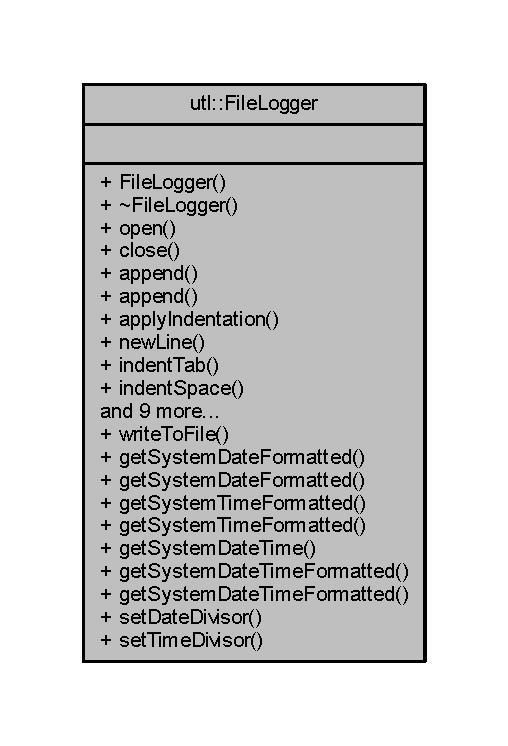
\includegraphics[width=247pt]{classutl_1_1_file_logger__coll__graph}
\end{center}
\end{figure}
\subsection*{Public Member Functions}
\begin{DoxyCompactItemize}
\item 
\mbox{\hyperlink{classutl_1_1_file_logger_af863c2a6176181b6c252ff91a46760fa}{File\+Logger}} ()
\item 
\mbox{\hyperlink{classutl_1_1_file_logger_a2bbc4a7a41145e14efaafb9563a8a869}{$\sim$\+File\+Logger}} ()
\item 
void \mbox{\hyperlink{classutl_1_1_file_logger_affe578f56cb67c168db89edf6b93497f}{Open}} (const char $\ast$filepath)
\item 
void \mbox{\hyperlink{classutl_1_1_file_logger_a1df768e7a0615fdbb6bf8d3a9b459c75}{Close}} ()
\item 
{\footnotesize template$<$class T , class... Args$>$ }\\void \mbox{\hyperlink{classutl_1_1_file_logger_aafcfaedf7477ef92fa0bfc9153b06fdb}{Append}} (T arg, Args... args)
\item 
{\footnotesize template$<$class T $>$ }\\void \mbox{\hyperlink{classutl_1_1_file_logger_a04df8807b424079163a1f6780ea339ef}{Append}} (T arg)
\item 
void \mbox{\hyperlink{classutl_1_1_file_logger_a27f64e20da2b923600fd3fda9b1ebf44}{Apply\+Indentation}} ()
\item 
void \mbox{\hyperlink{classutl_1_1_file_logger_ae4a25d385148ae2ebb310e779a23c4aa}{New\+Line}} ()
\item 
void \mbox{\hyperlink{classutl_1_1_file_logger_a286c8ae460735757b7948cf99d418ed5}{Indent\+Tab}} (const unsigned int steps)
\item 
void \mbox{\hyperlink{classutl_1_1_file_logger_ab714a77af672c562512044198be30885}{Indent\+Space}} (const unsigned int spaces)
\item 
void \mbox{\hyperlink{classutl_1_1_file_logger_aec7cd859010754605ecbcded93815eca}{Set\+Indentation\+Fill}} (const char fill\+Char)
\item 
char \mbox{\hyperlink{classutl_1_1_file_logger_a1352f5759c245eec3650271dd7b10459}{Get\+Indentation\+Fill}} () const
\item 
void \mbox{\hyperlink{classutl_1_1_file_logger_a8ee37650826800cf02719c2e67d1bc16}{Indent\+Reverse\+Tab}} (const unsigned int steps)
\item 
void \mbox{\hyperlink{classutl_1_1_file_logger_aae921d2a4b24dd2639575208f101ac4a}{Indent\+Reverse\+Space}} (const unsigned int spaces)
\item 
void \mbox{\hyperlink{classutl_1_1_file_logger_a5cc294f87e85875a5ec420bf4b60f944}{Reset\+Indentation}} ()
\item 
unsigned int \mbox{\hyperlink{classutl_1_1_file_logger_ad9a89d0c4453cff4d48253d09020daf8}{Get\+Current\+Indentation}} () const
\item 
void \mbox{\hyperlink{classutl_1_1_file_logger_ae8ce6a73b455cf5b865121ded27813d7}{Set\+Indentation}} (const unsigned int indentation)
\item 
unsigned int \mbox{\hyperlink{classutl_1_1_file_logger_a309e5f94ba4c5ea6e41bb7c600682e38}{Get\+Indentation\+Step}} () const
\item 
void \mbox{\hyperlink{classutl_1_1_file_logger_a69d64f348cae396095f6b4cff1955636}{Set\+Indentation\+Step}} (const unsigned int step)
\end{DoxyCompactItemize}
\subsection*{Static Public Member Functions}
\begin{DoxyCompactItemize}
\item 
static void \mbox{\hyperlink{classutl_1_1_file_logger_a05b05806b51da47772c9af14c4dabf41}{Write\+To\+File}} (const char $\ast$filepath, const char $\ast$data)
\item 
static std\+::string \mbox{\hyperlink{classutl_1_1_file_logger_a1346d06e73a06269bc75dd8a7f007f7a}{Get\+System\+Date\+Formatted}} ()
\item 
static std\+::string \mbox{\hyperlink{classutl_1_1_file_logger_a6d86887d521a139f467cd8a68170a56b}{Get\+System\+Date\+Formatted}} (const char divider)
\item 
static std\+::string \mbox{\hyperlink{classutl_1_1_file_logger_a5333d4596df47edfe4e625aca913d89b}{Get\+System\+Time\+Formatted}} ()
\item 
static std\+::string \mbox{\hyperlink{classutl_1_1_file_logger_ac5bee0b767adbe81ad20ce93b750c971}{Get\+System\+Time\+Formatted}} (const char divider)
\item 
static tm \mbox{\hyperlink{classutl_1_1_file_logger_ac22f71f18b679450b591edc05baa8956}{Get\+System\+Date\+Time}} ()
\item 
static std\+::string \mbox{\hyperlink{classutl_1_1_file_logger_a3287f373cc5a9766637eaad183d7eb88}{Get\+System\+Date\+Time\+Formatted}} ()
\item 
static std\+::string \mbox{\hyperlink{classutl_1_1_file_logger_a6819ec578b8a8605d3b3f47d91a30a3f}{Get\+System\+Date\+Time\+Formatted}} (const char date\+Divider, const char date\+Time\+Divider, const char time\+Divider)
\item 
static void \mbox{\hyperlink{classutl_1_1_file_logger_a273c189bbb9dc395462c01a63e318b7c}{Set\+Date\+Divisor}} (const char divider)
\item 
static void \mbox{\hyperlink{classutl_1_1_file_logger_a4a683c7f8d2a08e42be4688f8f117a05}{Set\+Time\+Divisor}} (const char divider)
\end{DoxyCompactItemize}


\subsection{Constructor \& Destructor Documentation}
\mbox{\Hypertarget{classutl_1_1_file_logger_af863c2a6176181b6c252ff91a46760fa}\label{classutl_1_1_file_logger_af863c2a6176181b6c252ff91a46760fa}} 
\index{utl\+::\+File\+Logger@{utl\+::\+File\+Logger}!File\+Logger@{File\+Logger}}
\index{File\+Logger@{File\+Logger}!utl\+::\+File\+Logger@{utl\+::\+File\+Logger}}
\subsubsection{\texorpdfstring{File\+Logger()}{FileLogger()}}
{\footnotesize\ttfamily utl\+::\+File\+Logger\+::\+File\+Logger (\begin{DoxyParamCaption}{ }\end{DoxyParamCaption})}

\mbox{\Hypertarget{classutl_1_1_file_logger_a2bbc4a7a41145e14efaafb9563a8a869}\label{classutl_1_1_file_logger_a2bbc4a7a41145e14efaafb9563a8a869}} 
\index{utl\+::\+File\+Logger@{utl\+::\+File\+Logger}!````~File\+Logger@{$\sim$\+File\+Logger}}
\index{````~File\+Logger@{$\sim$\+File\+Logger}!utl\+::\+File\+Logger@{utl\+::\+File\+Logger}}
\subsubsection{\texorpdfstring{$\sim$\+File\+Logger()}{~FileLogger()}}
{\footnotesize\ttfamily utl\+::\+File\+Logger\+::$\sim$\+File\+Logger (\begin{DoxyParamCaption}{ }\end{DoxyParamCaption})}



\subsection{Member Function Documentation}
\mbox{\Hypertarget{classutl_1_1_file_logger_aafcfaedf7477ef92fa0bfc9153b06fdb}\label{classutl_1_1_file_logger_aafcfaedf7477ef92fa0bfc9153b06fdb}} 
\index{utl\+::\+File\+Logger@{utl\+::\+File\+Logger}!Append@{Append}}
\index{Append@{Append}!utl\+::\+File\+Logger@{utl\+::\+File\+Logger}}
\subsubsection{\texorpdfstring{Append()}{Append()}\hspace{0.1cm}{\footnotesize\ttfamily [1/2]}}
{\footnotesize\ttfamily template$<$class T , class... Args$>$ \\
void utl\+::\+File\+Logger\+::\+Append (\begin{DoxyParamCaption}\item[{T}]{arg,  }\item[{Args...}]{args }\end{DoxyParamCaption})}

\mbox{\Hypertarget{classutl_1_1_file_logger_a04df8807b424079163a1f6780ea339ef}\label{classutl_1_1_file_logger_a04df8807b424079163a1f6780ea339ef}} 
\index{utl\+::\+File\+Logger@{utl\+::\+File\+Logger}!Append@{Append}}
\index{Append@{Append}!utl\+::\+File\+Logger@{utl\+::\+File\+Logger}}
\subsubsection{\texorpdfstring{Append()}{Append()}\hspace{0.1cm}{\footnotesize\ttfamily [2/2]}}
{\footnotesize\ttfamily template$<$class T $>$ \\
void utl\+::\+File\+Logger\+::\+Append (\begin{DoxyParamCaption}\item[{T}]{arg }\end{DoxyParamCaption})}

\mbox{\Hypertarget{classutl_1_1_file_logger_a27f64e20da2b923600fd3fda9b1ebf44}\label{classutl_1_1_file_logger_a27f64e20da2b923600fd3fda9b1ebf44}} 
\index{utl\+::\+File\+Logger@{utl\+::\+File\+Logger}!Apply\+Indentation@{Apply\+Indentation}}
\index{Apply\+Indentation@{Apply\+Indentation}!utl\+::\+File\+Logger@{utl\+::\+File\+Logger}}
\subsubsection{\texorpdfstring{Apply\+Indentation()}{ApplyIndentation()}}
{\footnotesize\ttfamily void utl\+::\+File\+Logger\+::\+Apply\+Indentation (\begin{DoxyParamCaption}{ }\end{DoxyParamCaption})}

\mbox{\Hypertarget{classutl_1_1_file_logger_a1df768e7a0615fdbb6bf8d3a9b459c75}\label{classutl_1_1_file_logger_a1df768e7a0615fdbb6bf8d3a9b459c75}} 
\index{utl\+::\+File\+Logger@{utl\+::\+File\+Logger}!Close@{Close}}
\index{Close@{Close}!utl\+::\+File\+Logger@{utl\+::\+File\+Logger}}
\subsubsection{\texorpdfstring{Close()}{Close()}}
{\footnotesize\ttfamily void utl\+::\+File\+Logger\+::\+Close (\begin{DoxyParamCaption}{ }\end{DoxyParamCaption})}

\mbox{\Hypertarget{classutl_1_1_file_logger_ad9a89d0c4453cff4d48253d09020daf8}\label{classutl_1_1_file_logger_ad9a89d0c4453cff4d48253d09020daf8}} 
\index{utl\+::\+File\+Logger@{utl\+::\+File\+Logger}!Get\+Current\+Indentation@{Get\+Current\+Indentation}}
\index{Get\+Current\+Indentation@{Get\+Current\+Indentation}!utl\+::\+File\+Logger@{utl\+::\+File\+Logger}}
\subsubsection{\texorpdfstring{Get\+Current\+Indentation()}{GetCurrentIndentation()}}
{\footnotesize\ttfamily unsigned int utl\+::\+File\+Logger\+::\+Get\+Current\+Indentation (\begin{DoxyParamCaption}{ }\end{DoxyParamCaption}) const}

\mbox{\Hypertarget{classutl_1_1_file_logger_a1352f5759c245eec3650271dd7b10459}\label{classutl_1_1_file_logger_a1352f5759c245eec3650271dd7b10459}} 
\index{utl\+::\+File\+Logger@{utl\+::\+File\+Logger}!Get\+Indentation\+Fill@{Get\+Indentation\+Fill}}
\index{Get\+Indentation\+Fill@{Get\+Indentation\+Fill}!utl\+::\+File\+Logger@{utl\+::\+File\+Logger}}
\subsubsection{\texorpdfstring{Get\+Indentation\+Fill()}{GetIndentationFill()}}
{\footnotesize\ttfamily char utl\+::\+File\+Logger\+::\+Get\+Indentation\+Fill (\begin{DoxyParamCaption}{ }\end{DoxyParamCaption}) const}

\mbox{\Hypertarget{classutl_1_1_file_logger_a309e5f94ba4c5ea6e41bb7c600682e38}\label{classutl_1_1_file_logger_a309e5f94ba4c5ea6e41bb7c600682e38}} 
\index{utl\+::\+File\+Logger@{utl\+::\+File\+Logger}!Get\+Indentation\+Step@{Get\+Indentation\+Step}}
\index{Get\+Indentation\+Step@{Get\+Indentation\+Step}!utl\+::\+File\+Logger@{utl\+::\+File\+Logger}}
\subsubsection{\texorpdfstring{Get\+Indentation\+Step()}{GetIndentationStep()}}
{\footnotesize\ttfamily unsigned int utl\+::\+File\+Logger\+::\+Get\+Indentation\+Step (\begin{DoxyParamCaption}{ }\end{DoxyParamCaption}) const}

\mbox{\Hypertarget{classutl_1_1_file_logger_a1346d06e73a06269bc75dd8a7f007f7a}\label{classutl_1_1_file_logger_a1346d06e73a06269bc75dd8a7f007f7a}} 
\index{utl\+::\+File\+Logger@{utl\+::\+File\+Logger}!Get\+System\+Date\+Formatted@{Get\+System\+Date\+Formatted}}
\index{Get\+System\+Date\+Formatted@{Get\+System\+Date\+Formatted}!utl\+::\+File\+Logger@{utl\+::\+File\+Logger}}
\subsubsection{\texorpdfstring{Get\+System\+Date\+Formatted()}{GetSystemDateFormatted()}\hspace{0.1cm}{\footnotesize\ttfamily [1/2]}}
{\footnotesize\ttfamily std\+::string utl\+::\+File\+Logger\+::\+Get\+System\+Date\+Formatted (\begin{DoxyParamCaption}{ }\end{DoxyParamCaption})\hspace{0.3cm}{\ttfamily [static]}}

\mbox{\Hypertarget{classutl_1_1_file_logger_a6d86887d521a139f467cd8a68170a56b}\label{classutl_1_1_file_logger_a6d86887d521a139f467cd8a68170a56b}} 
\index{utl\+::\+File\+Logger@{utl\+::\+File\+Logger}!Get\+System\+Date\+Formatted@{Get\+System\+Date\+Formatted}}
\index{Get\+System\+Date\+Formatted@{Get\+System\+Date\+Formatted}!utl\+::\+File\+Logger@{utl\+::\+File\+Logger}}
\subsubsection{\texorpdfstring{Get\+System\+Date\+Formatted()}{GetSystemDateFormatted()}\hspace{0.1cm}{\footnotesize\ttfamily [2/2]}}
{\footnotesize\ttfamily std\+::string utl\+::\+File\+Logger\+::\+Get\+System\+Date\+Formatted (\begin{DoxyParamCaption}\item[{const char}]{divider }\end{DoxyParamCaption})\hspace{0.3cm}{\ttfamily [static]}}

\mbox{\Hypertarget{classutl_1_1_file_logger_ac22f71f18b679450b591edc05baa8956}\label{classutl_1_1_file_logger_ac22f71f18b679450b591edc05baa8956}} 
\index{utl\+::\+File\+Logger@{utl\+::\+File\+Logger}!Get\+System\+Date\+Time@{Get\+System\+Date\+Time}}
\index{Get\+System\+Date\+Time@{Get\+System\+Date\+Time}!utl\+::\+File\+Logger@{utl\+::\+File\+Logger}}
\subsubsection{\texorpdfstring{Get\+System\+Date\+Time()}{GetSystemDateTime()}}
{\footnotesize\ttfamily tm utl\+::\+File\+Logger\+::\+Get\+System\+Date\+Time (\begin{DoxyParamCaption}{ }\end{DoxyParamCaption})\hspace{0.3cm}{\ttfamily [static]}}

\mbox{\Hypertarget{classutl_1_1_file_logger_a3287f373cc5a9766637eaad183d7eb88}\label{classutl_1_1_file_logger_a3287f373cc5a9766637eaad183d7eb88}} 
\index{utl\+::\+File\+Logger@{utl\+::\+File\+Logger}!Get\+System\+Date\+Time\+Formatted@{Get\+System\+Date\+Time\+Formatted}}
\index{Get\+System\+Date\+Time\+Formatted@{Get\+System\+Date\+Time\+Formatted}!utl\+::\+File\+Logger@{utl\+::\+File\+Logger}}
\subsubsection{\texorpdfstring{Get\+System\+Date\+Time\+Formatted()}{GetSystemDateTimeFormatted()}\hspace{0.1cm}{\footnotesize\ttfamily [1/2]}}
{\footnotesize\ttfamily std\+::string utl\+::\+File\+Logger\+::\+Get\+System\+Date\+Time\+Formatted (\begin{DoxyParamCaption}{ }\end{DoxyParamCaption})\hspace{0.3cm}{\ttfamily [static]}}

\mbox{\Hypertarget{classutl_1_1_file_logger_a6819ec578b8a8605d3b3f47d91a30a3f}\label{classutl_1_1_file_logger_a6819ec578b8a8605d3b3f47d91a30a3f}} 
\index{utl\+::\+File\+Logger@{utl\+::\+File\+Logger}!Get\+System\+Date\+Time\+Formatted@{Get\+System\+Date\+Time\+Formatted}}
\index{Get\+System\+Date\+Time\+Formatted@{Get\+System\+Date\+Time\+Formatted}!utl\+::\+File\+Logger@{utl\+::\+File\+Logger}}
\subsubsection{\texorpdfstring{Get\+System\+Date\+Time\+Formatted()}{GetSystemDateTimeFormatted()}\hspace{0.1cm}{\footnotesize\ttfamily [2/2]}}
{\footnotesize\ttfamily std\+::string utl\+::\+File\+Logger\+::\+Get\+System\+Date\+Time\+Formatted (\begin{DoxyParamCaption}\item[{const char}]{date\+Divider,  }\item[{const char}]{date\+Time\+Divider,  }\item[{const char}]{time\+Divider }\end{DoxyParamCaption})\hspace{0.3cm}{\ttfamily [static]}}

\mbox{\Hypertarget{classutl_1_1_file_logger_a5333d4596df47edfe4e625aca913d89b}\label{classutl_1_1_file_logger_a5333d4596df47edfe4e625aca913d89b}} 
\index{utl\+::\+File\+Logger@{utl\+::\+File\+Logger}!Get\+System\+Time\+Formatted@{Get\+System\+Time\+Formatted}}
\index{Get\+System\+Time\+Formatted@{Get\+System\+Time\+Formatted}!utl\+::\+File\+Logger@{utl\+::\+File\+Logger}}
\subsubsection{\texorpdfstring{Get\+System\+Time\+Formatted()}{GetSystemTimeFormatted()}\hspace{0.1cm}{\footnotesize\ttfamily [1/2]}}
{\footnotesize\ttfamily std\+::string utl\+::\+File\+Logger\+::\+Get\+System\+Time\+Formatted (\begin{DoxyParamCaption}{ }\end{DoxyParamCaption})\hspace{0.3cm}{\ttfamily [static]}}

\mbox{\Hypertarget{classutl_1_1_file_logger_ac5bee0b767adbe81ad20ce93b750c971}\label{classutl_1_1_file_logger_ac5bee0b767adbe81ad20ce93b750c971}} 
\index{utl\+::\+File\+Logger@{utl\+::\+File\+Logger}!Get\+System\+Time\+Formatted@{Get\+System\+Time\+Formatted}}
\index{Get\+System\+Time\+Formatted@{Get\+System\+Time\+Formatted}!utl\+::\+File\+Logger@{utl\+::\+File\+Logger}}
\subsubsection{\texorpdfstring{Get\+System\+Time\+Formatted()}{GetSystemTimeFormatted()}\hspace{0.1cm}{\footnotesize\ttfamily [2/2]}}
{\footnotesize\ttfamily std\+::string utl\+::\+File\+Logger\+::\+Get\+System\+Time\+Formatted (\begin{DoxyParamCaption}\item[{const char}]{divider }\end{DoxyParamCaption})\hspace{0.3cm}{\ttfamily [static]}}

\mbox{\Hypertarget{classutl_1_1_file_logger_aae921d2a4b24dd2639575208f101ac4a}\label{classutl_1_1_file_logger_aae921d2a4b24dd2639575208f101ac4a}} 
\index{utl\+::\+File\+Logger@{utl\+::\+File\+Logger}!Indent\+Reverse\+Space@{Indent\+Reverse\+Space}}
\index{Indent\+Reverse\+Space@{Indent\+Reverse\+Space}!utl\+::\+File\+Logger@{utl\+::\+File\+Logger}}
\subsubsection{\texorpdfstring{Indent\+Reverse\+Space()}{IndentReverseSpace()}}
{\footnotesize\ttfamily void utl\+::\+File\+Logger\+::\+Indent\+Reverse\+Space (\begin{DoxyParamCaption}\item[{const unsigned int}]{spaces }\end{DoxyParamCaption})}

\mbox{\Hypertarget{classutl_1_1_file_logger_a8ee37650826800cf02719c2e67d1bc16}\label{classutl_1_1_file_logger_a8ee37650826800cf02719c2e67d1bc16}} 
\index{utl\+::\+File\+Logger@{utl\+::\+File\+Logger}!Indent\+Reverse\+Tab@{Indent\+Reverse\+Tab}}
\index{Indent\+Reverse\+Tab@{Indent\+Reverse\+Tab}!utl\+::\+File\+Logger@{utl\+::\+File\+Logger}}
\subsubsection{\texorpdfstring{Indent\+Reverse\+Tab()}{IndentReverseTab()}}
{\footnotesize\ttfamily void utl\+::\+File\+Logger\+::\+Indent\+Reverse\+Tab (\begin{DoxyParamCaption}\item[{const unsigned int}]{steps }\end{DoxyParamCaption})}

\mbox{\Hypertarget{classutl_1_1_file_logger_ab714a77af672c562512044198be30885}\label{classutl_1_1_file_logger_ab714a77af672c562512044198be30885}} 
\index{utl\+::\+File\+Logger@{utl\+::\+File\+Logger}!Indent\+Space@{Indent\+Space}}
\index{Indent\+Space@{Indent\+Space}!utl\+::\+File\+Logger@{utl\+::\+File\+Logger}}
\subsubsection{\texorpdfstring{Indent\+Space()}{IndentSpace()}}
{\footnotesize\ttfamily void utl\+::\+File\+Logger\+::\+Indent\+Space (\begin{DoxyParamCaption}\item[{const unsigned int}]{spaces }\end{DoxyParamCaption})}

\mbox{\Hypertarget{classutl_1_1_file_logger_a286c8ae460735757b7948cf99d418ed5}\label{classutl_1_1_file_logger_a286c8ae460735757b7948cf99d418ed5}} 
\index{utl\+::\+File\+Logger@{utl\+::\+File\+Logger}!Indent\+Tab@{Indent\+Tab}}
\index{Indent\+Tab@{Indent\+Tab}!utl\+::\+File\+Logger@{utl\+::\+File\+Logger}}
\subsubsection{\texorpdfstring{Indent\+Tab()}{IndentTab()}}
{\footnotesize\ttfamily void utl\+::\+File\+Logger\+::\+Indent\+Tab (\begin{DoxyParamCaption}\item[{const unsigned int}]{steps }\end{DoxyParamCaption})}

\mbox{\Hypertarget{classutl_1_1_file_logger_ae4a25d385148ae2ebb310e779a23c4aa}\label{classutl_1_1_file_logger_ae4a25d385148ae2ebb310e779a23c4aa}} 
\index{utl\+::\+File\+Logger@{utl\+::\+File\+Logger}!New\+Line@{New\+Line}}
\index{New\+Line@{New\+Line}!utl\+::\+File\+Logger@{utl\+::\+File\+Logger}}
\subsubsection{\texorpdfstring{New\+Line()}{NewLine()}}
{\footnotesize\ttfamily void utl\+::\+File\+Logger\+::\+New\+Line (\begin{DoxyParamCaption}{ }\end{DoxyParamCaption})}

\mbox{\Hypertarget{classutl_1_1_file_logger_affe578f56cb67c168db89edf6b93497f}\label{classutl_1_1_file_logger_affe578f56cb67c168db89edf6b93497f}} 
\index{utl\+::\+File\+Logger@{utl\+::\+File\+Logger}!Open@{Open}}
\index{Open@{Open}!utl\+::\+File\+Logger@{utl\+::\+File\+Logger}}
\subsubsection{\texorpdfstring{Open()}{Open()}}
{\footnotesize\ttfamily void utl\+::\+File\+Logger\+::\+Open (\begin{DoxyParamCaption}\item[{const char $\ast$}]{filepath }\end{DoxyParamCaption})}

\mbox{\Hypertarget{classutl_1_1_file_logger_a5cc294f87e85875a5ec420bf4b60f944}\label{classutl_1_1_file_logger_a5cc294f87e85875a5ec420bf4b60f944}} 
\index{utl\+::\+File\+Logger@{utl\+::\+File\+Logger}!Reset\+Indentation@{Reset\+Indentation}}
\index{Reset\+Indentation@{Reset\+Indentation}!utl\+::\+File\+Logger@{utl\+::\+File\+Logger}}
\subsubsection{\texorpdfstring{Reset\+Indentation()}{ResetIndentation()}}
{\footnotesize\ttfamily void utl\+::\+File\+Logger\+::\+Reset\+Indentation (\begin{DoxyParamCaption}{ }\end{DoxyParamCaption})}

\mbox{\Hypertarget{classutl_1_1_file_logger_a273c189bbb9dc395462c01a63e318b7c}\label{classutl_1_1_file_logger_a273c189bbb9dc395462c01a63e318b7c}} 
\index{utl\+::\+File\+Logger@{utl\+::\+File\+Logger}!Set\+Date\+Divisor@{Set\+Date\+Divisor}}
\index{Set\+Date\+Divisor@{Set\+Date\+Divisor}!utl\+::\+File\+Logger@{utl\+::\+File\+Logger}}
\subsubsection{\texorpdfstring{Set\+Date\+Divisor()}{SetDateDivisor()}}
{\footnotesize\ttfamily void utl\+::\+File\+Logger\+::\+Set\+Date\+Divisor (\begin{DoxyParamCaption}\item[{const char}]{divider }\end{DoxyParamCaption})\hspace{0.3cm}{\ttfamily [static]}}

\mbox{\Hypertarget{classutl_1_1_file_logger_ae8ce6a73b455cf5b865121ded27813d7}\label{classutl_1_1_file_logger_ae8ce6a73b455cf5b865121ded27813d7}} 
\index{utl\+::\+File\+Logger@{utl\+::\+File\+Logger}!Set\+Indentation@{Set\+Indentation}}
\index{Set\+Indentation@{Set\+Indentation}!utl\+::\+File\+Logger@{utl\+::\+File\+Logger}}
\subsubsection{\texorpdfstring{Set\+Indentation()}{SetIndentation()}}
{\footnotesize\ttfamily void utl\+::\+File\+Logger\+::\+Set\+Indentation (\begin{DoxyParamCaption}\item[{const unsigned int}]{indentation }\end{DoxyParamCaption})}

\mbox{\Hypertarget{classutl_1_1_file_logger_aec7cd859010754605ecbcded93815eca}\label{classutl_1_1_file_logger_aec7cd859010754605ecbcded93815eca}} 
\index{utl\+::\+File\+Logger@{utl\+::\+File\+Logger}!Set\+Indentation\+Fill@{Set\+Indentation\+Fill}}
\index{Set\+Indentation\+Fill@{Set\+Indentation\+Fill}!utl\+::\+File\+Logger@{utl\+::\+File\+Logger}}
\subsubsection{\texorpdfstring{Set\+Indentation\+Fill()}{SetIndentationFill()}}
{\footnotesize\ttfamily void utl\+::\+File\+Logger\+::\+Set\+Indentation\+Fill (\begin{DoxyParamCaption}\item[{const char}]{fill\+Char }\end{DoxyParamCaption})}

\mbox{\Hypertarget{classutl_1_1_file_logger_a69d64f348cae396095f6b4cff1955636}\label{classutl_1_1_file_logger_a69d64f348cae396095f6b4cff1955636}} 
\index{utl\+::\+File\+Logger@{utl\+::\+File\+Logger}!Set\+Indentation\+Step@{Set\+Indentation\+Step}}
\index{Set\+Indentation\+Step@{Set\+Indentation\+Step}!utl\+::\+File\+Logger@{utl\+::\+File\+Logger}}
\subsubsection{\texorpdfstring{Set\+Indentation\+Step()}{SetIndentationStep()}}
{\footnotesize\ttfamily void utl\+::\+File\+Logger\+::\+Set\+Indentation\+Step (\begin{DoxyParamCaption}\item[{const unsigned int}]{step }\end{DoxyParamCaption})}

\mbox{\Hypertarget{classutl_1_1_file_logger_a4a683c7f8d2a08e42be4688f8f117a05}\label{classutl_1_1_file_logger_a4a683c7f8d2a08e42be4688f8f117a05}} 
\index{utl\+::\+File\+Logger@{utl\+::\+File\+Logger}!Set\+Time\+Divisor@{Set\+Time\+Divisor}}
\index{Set\+Time\+Divisor@{Set\+Time\+Divisor}!utl\+::\+File\+Logger@{utl\+::\+File\+Logger}}
\subsubsection{\texorpdfstring{Set\+Time\+Divisor()}{SetTimeDivisor()}}
{\footnotesize\ttfamily void utl\+::\+File\+Logger\+::\+Set\+Time\+Divisor (\begin{DoxyParamCaption}\item[{const char}]{divider }\end{DoxyParamCaption})\hspace{0.3cm}{\ttfamily [static]}}

\mbox{\Hypertarget{classutl_1_1_file_logger_a05b05806b51da47772c9af14c4dabf41}\label{classutl_1_1_file_logger_a05b05806b51da47772c9af14c4dabf41}} 
\index{utl\+::\+File\+Logger@{utl\+::\+File\+Logger}!Write\+To\+File@{Write\+To\+File}}
\index{Write\+To\+File@{Write\+To\+File}!utl\+::\+File\+Logger@{utl\+::\+File\+Logger}}
\subsubsection{\texorpdfstring{Write\+To\+File()}{WriteToFile()}}
{\footnotesize\ttfamily void utl\+::\+File\+Logger\+::\+Write\+To\+File (\begin{DoxyParamCaption}\item[{const char $\ast$}]{filepath,  }\item[{const char $\ast$}]{data }\end{DoxyParamCaption})\hspace{0.3cm}{\ttfamily [static]}}



The documentation for this class was generated from the following files\+:\begin{DoxyCompactItemize}
\item 
D\+:/\+Library/\+Documents/\+Job/\+Forschungsmaster/\+Projekte/\+Eye\+Candy3\+D/\+Eye\+Candy3\+D/include/\+E\+C3\+D/\+Utilities/\mbox{\hyperlink{_file_logger_8h}{File\+Logger.\+h}}\item 
D\+:/\+Library/\+Documents/\+Job/\+Forschungsmaster/\+Projekte/\+Eye\+Candy3\+D/\+Eye\+Candy3\+D/src/\+Utilities/\mbox{\hyperlink{_file_logger_8cpp}{File\+Logger.\+cpp}}\end{DoxyCompactItemize}

\hypertarget{structec_1_1_focus_event}{}\section{ec\+:\+:Focus\+Event Struct Reference}
\label{structec_1_1_focus_event}\index{ec\+::\+Focus\+Event@{ec\+::\+Focus\+Event}}


{\ttfamily \#include $<$Input\+Event.\+h$>$}



Collaboration diagram for ec\+:\+:Focus\+Event\+:\nopagebreak
\begin{figure}[H]
\begin{center}
\leavevmode
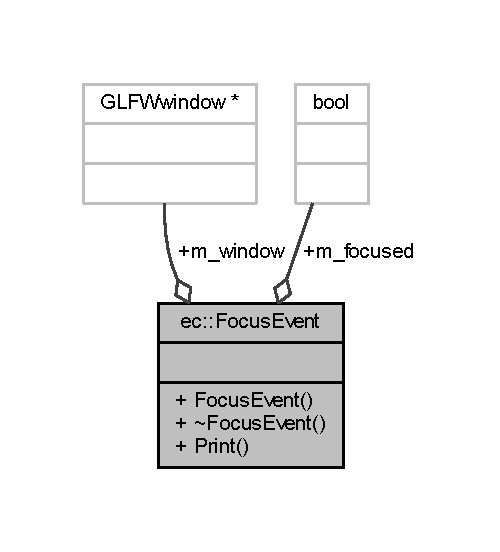
\includegraphics[width=240pt]{structec_1_1_focus_event__coll__graph}
\end{center}
\end{figure}
\subsection*{Public Member Functions}
\begin{DoxyCompactItemize}
\item 
\mbox{\hyperlink{structec_1_1_focus_event_ab160b94dd4af651dacdd6049cfdabe0a}{Focus\+Event}} (G\+L\+F\+Wwindow $\ast$window, const bool focused)
\item 
\mbox{\hyperlink{structec_1_1_focus_event_ab59b3bde4ad39accab7fadd830b5f226}{$\sim$\+Focus\+Event}} ()
\item 
void \mbox{\hyperlink{structec_1_1_focus_event_a31a1f08d96f83cbb906f92be18bc8bfb}{Print}} () const
\end{DoxyCompactItemize}
\subsection*{Public Attributes}
\begin{DoxyCompactItemize}
\item 
G\+L\+F\+Wwindow $\ast$ \mbox{\hyperlink{structec_1_1_focus_event_a44db4d7190f7312e23a56cf90c634187}{m\+\_\+window}}
\item 
bool \mbox{\hyperlink{structec_1_1_focus_event_afbca9e2277612590e35c63ef3c445042}{m\+\_\+focused}}
\end{DoxyCompactItemize}


\subsection{Constructor \& Destructor Documentation}
\mbox{\Hypertarget{structec_1_1_focus_event_ab160b94dd4af651dacdd6049cfdabe0a}\label{structec_1_1_focus_event_ab160b94dd4af651dacdd6049cfdabe0a}} 
\index{ec\+::\+Focus\+Event@{ec\+::\+Focus\+Event}!Focus\+Event@{Focus\+Event}}
\index{Focus\+Event@{Focus\+Event}!ec\+::\+Focus\+Event@{ec\+::\+Focus\+Event}}
\subsubsection{\texorpdfstring{Focus\+Event()}{FocusEvent()}}
{\footnotesize\ttfamily ec\+::\+Focus\+Event\+::\+Focus\+Event (\begin{DoxyParamCaption}\item[{G\+L\+F\+Wwindow $\ast$}]{window,  }\item[{const bool}]{focused }\end{DoxyParamCaption})}

\mbox{\Hypertarget{structec_1_1_focus_event_ab59b3bde4ad39accab7fadd830b5f226}\label{structec_1_1_focus_event_ab59b3bde4ad39accab7fadd830b5f226}} 
\index{ec\+::\+Focus\+Event@{ec\+::\+Focus\+Event}!````~Focus\+Event@{$\sim$\+Focus\+Event}}
\index{````~Focus\+Event@{$\sim$\+Focus\+Event}!ec\+::\+Focus\+Event@{ec\+::\+Focus\+Event}}
\subsubsection{\texorpdfstring{$\sim$\+Focus\+Event()}{~FocusEvent()}}
{\footnotesize\ttfamily ec\+::\+Focus\+Event\+::$\sim$\+Focus\+Event (\begin{DoxyParamCaption}{ }\end{DoxyParamCaption})}



\subsection{Member Function Documentation}
\mbox{\Hypertarget{structec_1_1_focus_event_a31a1f08d96f83cbb906f92be18bc8bfb}\label{structec_1_1_focus_event_a31a1f08d96f83cbb906f92be18bc8bfb}} 
\index{ec\+::\+Focus\+Event@{ec\+::\+Focus\+Event}!Print@{Print}}
\index{Print@{Print}!ec\+::\+Focus\+Event@{ec\+::\+Focus\+Event}}
\subsubsection{\texorpdfstring{Print()}{Print()}}
{\footnotesize\ttfamily void ec\+::\+Focus\+Event\+::\+Print (\begin{DoxyParamCaption}{ }\end{DoxyParamCaption}) const}



\subsection{Member Data Documentation}
\mbox{\Hypertarget{structec_1_1_focus_event_afbca9e2277612590e35c63ef3c445042}\label{structec_1_1_focus_event_afbca9e2277612590e35c63ef3c445042}} 
\index{ec\+::\+Focus\+Event@{ec\+::\+Focus\+Event}!m\+\_\+focused@{m\+\_\+focused}}
\index{m\+\_\+focused@{m\+\_\+focused}!ec\+::\+Focus\+Event@{ec\+::\+Focus\+Event}}
\subsubsection{\texorpdfstring{m\+\_\+focused}{m\_focused}}
{\footnotesize\ttfamily bool ec\+::\+Focus\+Event\+::m\+\_\+focused}

\mbox{\Hypertarget{structec_1_1_focus_event_a44db4d7190f7312e23a56cf90c634187}\label{structec_1_1_focus_event_a44db4d7190f7312e23a56cf90c634187}} 
\index{ec\+::\+Focus\+Event@{ec\+::\+Focus\+Event}!m\+\_\+window@{m\+\_\+window}}
\index{m\+\_\+window@{m\+\_\+window}!ec\+::\+Focus\+Event@{ec\+::\+Focus\+Event}}
\subsubsection{\texorpdfstring{m\+\_\+window}{m\_window}}
{\footnotesize\ttfamily G\+L\+F\+Wwindow$\ast$ ec\+::\+Focus\+Event\+::m\+\_\+window}



The documentation for this struct was generated from the following files\+:\begin{DoxyCompactItemize}
\item 
D\+:/\+Library/\+Documents/\+Job/\+Forschungsmaster/\+Projekte/\+Eye\+Candy3\+D/\+Eye\+Candy3\+D/include/\+E\+C3\+D/\+Core/\mbox{\hyperlink{_input_event_8h}{Input\+Event.\+h}}\item 
D\+:/\+Library/\+Documents/\+Job/\+Forschungsmaster/\+Projekte/\+Eye\+Candy3\+D/\+Eye\+Candy3\+D/src/\+Core/\mbox{\hyperlink{_input_event_8cpp}{Input\+Event.\+cpp}}\end{DoxyCompactItemize}

\hypertarget{structec_1_1_font_character}{}\section{ec\+:\+:Font\+Character Struct Reference}
\label{structec_1_1_font_character}\index{ec\+::\+Font\+Character@{ec\+::\+Font\+Character}}


A font character holds information about a specific character of a specific font.  




{\ttfamily \#include $<$Font\+Character.\+h$>$}



Collaboration diagram for ec\+:\+:Font\+Character\+:\nopagebreak
\begin{figure}[H]
\begin{center}
\leavevmode
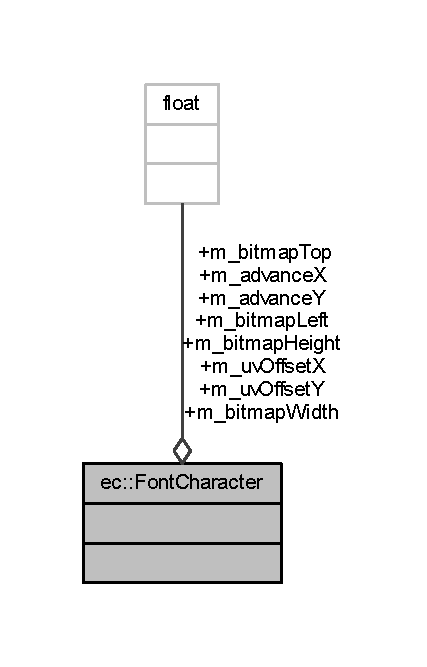
\includegraphics[width=205pt]{structec_1_1_font_character__coll__graph}
\end{center}
\end{figure}
\subsection*{Public Attributes}
\begin{DoxyCompactItemize}
\item 
float \mbox{\hyperlink{structec_1_1_font_character_a3dfcbeba30562b00daf057ac7d23c762}{m\+\_\+advanceX}}
\item 
float \mbox{\hyperlink{structec_1_1_font_character_afea51e45e05b1ac9bcf351184dde2286}{m\+\_\+advanceY}}
\item 
float \mbox{\hyperlink{structec_1_1_font_character_a29e1802582b887199a7c3484f7e99b09}{m\+\_\+bitmap\+Width}}
\item 
float \mbox{\hyperlink{structec_1_1_font_character_a4ab090e6a8358c152e94a931fe651423}{m\+\_\+bitmap\+Height}}
\item 
float \mbox{\hyperlink{structec_1_1_font_character_a5f666f5036f0ddf417c1b1e3475e433c}{m\+\_\+bitmap\+Left}}
\item 
float \mbox{\hyperlink{structec_1_1_font_character_a1555f3f60ade4c5a6a22f73d68710958}{m\+\_\+bitmap\+Top}}
\item 
float \mbox{\hyperlink{structec_1_1_font_character_a13e3f7cbc190b61581c6909bff262133}{m\+\_\+uv\+OffsetX}}
\item 
float \mbox{\hyperlink{structec_1_1_font_character_ac48d060931b82412610d9749b1374db3}{m\+\_\+uv\+OffsetY}}
\end{DoxyCompactItemize}


\subsection{Detailed Description}
A font character holds information about a specific character of a specific font. 

\subsection{Member Data Documentation}
\mbox{\Hypertarget{structec_1_1_font_character_a3dfcbeba30562b00daf057ac7d23c762}\label{structec_1_1_font_character_a3dfcbeba30562b00daf057ac7d23c762}} 
\index{ec\+::\+Font\+Character@{ec\+::\+Font\+Character}!m\+\_\+advanceX@{m\+\_\+advanceX}}
\index{m\+\_\+advanceX@{m\+\_\+advanceX}!ec\+::\+Font\+Character@{ec\+::\+Font\+Character}}
\subsubsection{\texorpdfstring{m\+\_\+advanceX}{m\_advanceX}}
{\footnotesize\ttfamily float ec\+::\+Font\+Character\+::m\+\_\+advanceX}

\mbox{\Hypertarget{structec_1_1_font_character_afea51e45e05b1ac9bcf351184dde2286}\label{structec_1_1_font_character_afea51e45e05b1ac9bcf351184dde2286}} 
\index{ec\+::\+Font\+Character@{ec\+::\+Font\+Character}!m\+\_\+advanceY@{m\+\_\+advanceY}}
\index{m\+\_\+advanceY@{m\+\_\+advanceY}!ec\+::\+Font\+Character@{ec\+::\+Font\+Character}}
\subsubsection{\texorpdfstring{m\+\_\+advanceY}{m\_advanceY}}
{\footnotesize\ttfamily float ec\+::\+Font\+Character\+::m\+\_\+advanceY}

\mbox{\Hypertarget{structec_1_1_font_character_a4ab090e6a8358c152e94a931fe651423}\label{structec_1_1_font_character_a4ab090e6a8358c152e94a931fe651423}} 
\index{ec\+::\+Font\+Character@{ec\+::\+Font\+Character}!m\+\_\+bitmap\+Height@{m\+\_\+bitmap\+Height}}
\index{m\+\_\+bitmap\+Height@{m\+\_\+bitmap\+Height}!ec\+::\+Font\+Character@{ec\+::\+Font\+Character}}
\subsubsection{\texorpdfstring{m\+\_\+bitmap\+Height}{m\_bitmapHeight}}
{\footnotesize\ttfamily float ec\+::\+Font\+Character\+::m\+\_\+bitmap\+Height}

\mbox{\Hypertarget{structec_1_1_font_character_a5f666f5036f0ddf417c1b1e3475e433c}\label{structec_1_1_font_character_a5f666f5036f0ddf417c1b1e3475e433c}} 
\index{ec\+::\+Font\+Character@{ec\+::\+Font\+Character}!m\+\_\+bitmap\+Left@{m\+\_\+bitmap\+Left}}
\index{m\+\_\+bitmap\+Left@{m\+\_\+bitmap\+Left}!ec\+::\+Font\+Character@{ec\+::\+Font\+Character}}
\subsubsection{\texorpdfstring{m\+\_\+bitmap\+Left}{m\_bitmapLeft}}
{\footnotesize\ttfamily float ec\+::\+Font\+Character\+::m\+\_\+bitmap\+Left}

\mbox{\Hypertarget{structec_1_1_font_character_a1555f3f60ade4c5a6a22f73d68710958}\label{structec_1_1_font_character_a1555f3f60ade4c5a6a22f73d68710958}} 
\index{ec\+::\+Font\+Character@{ec\+::\+Font\+Character}!m\+\_\+bitmap\+Top@{m\+\_\+bitmap\+Top}}
\index{m\+\_\+bitmap\+Top@{m\+\_\+bitmap\+Top}!ec\+::\+Font\+Character@{ec\+::\+Font\+Character}}
\subsubsection{\texorpdfstring{m\+\_\+bitmap\+Top}{m\_bitmapTop}}
{\footnotesize\ttfamily float ec\+::\+Font\+Character\+::m\+\_\+bitmap\+Top}

\mbox{\Hypertarget{structec_1_1_font_character_a29e1802582b887199a7c3484f7e99b09}\label{structec_1_1_font_character_a29e1802582b887199a7c3484f7e99b09}} 
\index{ec\+::\+Font\+Character@{ec\+::\+Font\+Character}!m\+\_\+bitmap\+Width@{m\+\_\+bitmap\+Width}}
\index{m\+\_\+bitmap\+Width@{m\+\_\+bitmap\+Width}!ec\+::\+Font\+Character@{ec\+::\+Font\+Character}}
\subsubsection{\texorpdfstring{m\+\_\+bitmap\+Width}{m\_bitmapWidth}}
{\footnotesize\ttfamily float ec\+::\+Font\+Character\+::m\+\_\+bitmap\+Width}

\mbox{\Hypertarget{structec_1_1_font_character_a13e3f7cbc190b61581c6909bff262133}\label{structec_1_1_font_character_a13e3f7cbc190b61581c6909bff262133}} 
\index{ec\+::\+Font\+Character@{ec\+::\+Font\+Character}!m\+\_\+uv\+OffsetX@{m\+\_\+uv\+OffsetX}}
\index{m\+\_\+uv\+OffsetX@{m\+\_\+uv\+OffsetX}!ec\+::\+Font\+Character@{ec\+::\+Font\+Character}}
\subsubsection{\texorpdfstring{m\+\_\+uv\+OffsetX}{m\_uvOffsetX}}
{\footnotesize\ttfamily float ec\+::\+Font\+Character\+::m\+\_\+uv\+OffsetX}

\mbox{\Hypertarget{structec_1_1_font_character_ac48d060931b82412610d9749b1374db3}\label{structec_1_1_font_character_ac48d060931b82412610d9749b1374db3}} 
\index{ec\+::\+Font\+Character@{ec\+::\+Font\+Character}!m\+\_\+uv\+OffsetY@{m\+\_\+uv\+OffsetY}}
\index{m\+\_\+uv\+OffsetY@{m\+\_\+uv\+OffsetY}!ec\+::\+Font\+Character@{ec\+::\+Font\+Character}}
\subsubsection{\texorpdfstring{m\+\_\+uv\+OffsetY}{m\_uvOffsetY}}
{\footnotesize\ttfamily float ec\+::\+Font\+Character\+::m\+\_\+uv\+OffsetY}



The documentation for this struct was generated from the following file\+:\begin{DoxyCompactItemize}
\item 
C\+:/\+Library/\+Job/\+Projekte/\+Simulation\+Visualization/\+Eye\+Candy3\+D/\+Eye\+Candy3\+D/include/\+E\+C3\+D/\+Core/\mbox{\hyperlink{_font_character_8h}{Font\+Character.\+h}}\end{DoxyCompactItemize}

\hypertarget{classec_1_1_font_texture_atlas}{}\section{ec\+:\+:Font\+Texture\+Atlas Class Reference}
\label{classec_1_1_font_texture_atlas}\index{ec\+::\+Font\+Texture\+Atlas@{ec\+::\+Font\+Texture\+Atlas}}


{\ttfamily \#include $<$Font\+Texture\+Atlas.\+h$>$}



Collaboration diagram for ec\+:\+:Font\+Texture\+Atlas\+:\nopagebreak
\begin{figure}[H]
\begin{center}
\leavevmode
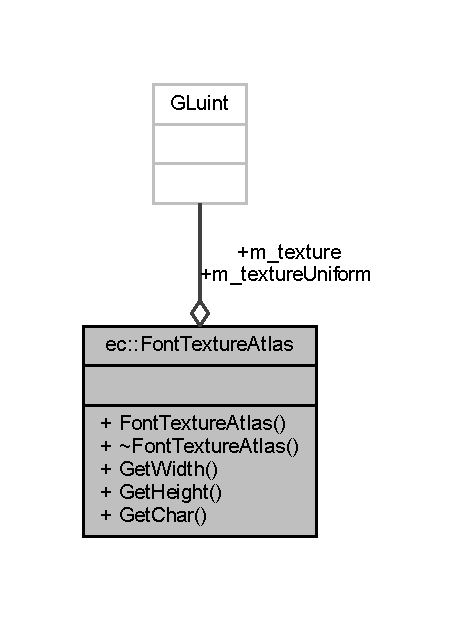
\includegraphics[width=219pt]{classec_1_1_font_texture_atlas__coll__graph}
\end{center}
\end{figure}
\subsection*{Public Member Functions}
\begin{DoxyCompactItemize}
\item 
\mbox{\hyperlink{classec_1_1_font_texture_atlas_abf42f99b2562130eb9b347c895cf14f3}{Font\+Texture\+Atlas}} (F\+T\+\_\+\+Face face, int h, G\+Luint t\+Uniform)
\item 
\mbox{\hyperlink{classec_1_1_font_texture_atlas_a9e520505ca5bd5b9cabe27448d285449}{$\sim$\+Font\+Texture\+Atlas}} ()
\item 
int \mbox{\hyperlink{classec_1_1_font_texture_atlas_a9259106785594dcf52a86120faf2abdf}{get\+Width}} () const
\item 
int \mbox{\hyperlink{classec_1_1_font_texture_atlas_aa6e4a6f124b7fed58783c48c78300244}{get\+Height}} () const
\item 
const \mbox{\hyperlink{structec_1_1_font_character}{Font\+Character}} \& \mbox{\hyperlink{classec_1_1_font_texture_atlas_a4587f2074d6295364a6ab7bac4a5846d}{get\+Char}} (int index) const
\end{DoxyCompactItemize}
\subsection*{Public Attributes}
\begin{DoxyCompactItemize}
\item 
G\+Luint \mbox{\hyperlink{classec_1_1_font_texture_atlas_a97620bab980c2f73e90928c1c9ec405a}{m\+\_\+texture}}
\item 
G\+Luint \mbox{\hyperlink{classec_1_1_font_texture_atlas_a0ad591b30c2e288d31f4ab9e18acb887}{m\+\_\+texture\+Uniform}}
\end{DoxyCompactItemize}


\subsection{Constructor \& Destructor Documentation}
\mbox{\Hypertarget{classec_1_1_font_texture_atlas_abf42f99b2562130eb9b347c895cf14f3}\label{classec_1_1_font_texture_atlas_abf42f99b2562130eb9b347c895cf14f3}} 
\index{ec\+::\+Font\+Texture\+Atlas@{ec\+::\+Font\+Texture\+Atlas}!Font\+Texture\+Atlas@{Font\+Texture\+Atlas}}
\index{Font\+Texture\+Atlas@{Font\+Texture\+Atlas}!ec\+::\+Font\+Texture\+Atlas@{ec\+::\+Font\+Texture\+Atlas}}
\subsubsection{\texorpdfstring{Font\+Texture\+Atlas()}{FontTextureAtlas()}}
{\footnotesize\ttfamily ec\+::\+Font\+Texture\+Atlas\+::\+Font\+Texture\+Atlas (\begin{DoxyParamCaption}\item[{F\+T\+\_\+\+Face}]{face,  }\item[{int}]{h,  }\item[{G\+Luint}]{t\+Uniform }\end{DoxyParamCaption})}

\mbox{\Hypertarget{classec_1_1_font_texture_atlas_a9e520505ca5bd5b9cabe27448d285449}\label{classec_1_1_font_texture_atlas_a9e520505ca5bd5b9cabe27448d285449}} 
\index{ec\+::\+Font\+Texture\+Atlas@{ec\+::\+Font\+Texture\+Atlas}!````~Font\+Texture\+Atlas@{$\sim$\+Font\+Texture\+Atlas}}
\index{````~Font\+Texture\+Atlas@{$\sim$\+Font\+Texture\+Atlas}!ec\+::\+Font\+Texture\+Atlas@{ec\+::\+Font\+Texture\+Atlas}}
\subsubsection{\texorpdfstring{$\sim$\+Font\+Texture\+Atlas()}{~FontTextureAtlas()}}
{\footnotesize\ttfamily ec\+::\+Font\+Texture\+Atlas\+::$\sim$\+Font\+Texture\+Atlas (\begin{DoxyParamCaption}{ }\end{DoxyParamCaption})}



\subsection{Member Function Documentation}
\mbox{\Hypertarget{classec_1_1_font_texture_atlas_a4587f2074d6295364a6ab7bac4a5846d}\label{classec_1_1_font_texture_atlas_a4587f2074d6295364a6ab7bac4a5846d}} 
\index{ec\+::\+Font\+Texture\+Atlas@{ec\+::\+Font\+Texture\+Atlas}!get\+Char@{get\+Char}}
\index{get\+Char@{get\+Char}!ec\+::\+Font\+Texture\+Atlas@{ec\+::\+Font\+Texture\+Atlas}}
\subsubsection{\texorpdfstring{get\+Char()}{getChar()}}
{\footnotesize\ttfamily const \mbox{\hyperlink{structec_1_1_font_character}{Font\+Character}} \& ec\+::\+Font\+Texture\+Atlas\+::get\+Char (\begin{DoxyParamCaption}\item[{int}]{index }\end{DoxyParamCaption}) const}

\mbox{\Hypertarget{classec_1_1_font_texture_atlas_aa6e4a6f124b7fed58783c48c78300244}\label{classec_1_1_font_texture_atlas_aa6e4a6f124b7fed58783c48c78300244}} 
\index{ec\+::\+Font\+Texture\+Atlas@{ec\+::\+Font\+Texture\+Atlas}!get\+Height@{get\+Height}}
\index{get\+Height@{get\+Height}!ec\+::\+Font\+Texture\+Atlas@{ec\+::\+Font\+Texture\+Atlas}}
\subsubsection{\texorpdfstring{get\+Height()}{getHeight()}}
{\footnotesize\ttfamily int ec\+::\+Font\+Texture\+Atlas\+::get\+Height (\begin{DoxyParamCaption}{ }\end{DoxyParamCaption}) const}

\mbox{\Hypertarget{classec_1_1_font_texture_atlas_a9259106785594dcf52a86120faf2abdf}\label{classec_1_1_font_texture_atlas_a9259106785594dcf52a86120faf2abdf}} 
\index{ec\+::\+Font\+Texture\+Atlas@{ec\+::\+Font\+Texture\+Atlas}!get\+Width@{get\+Width}}
\index{get\+Width@{get\+Width}!ec\+::\+Font\+Texture\+Atlas@{ec\+::\+Font\+Texture\+Atlas}}
\subsubsection{\texorpdfstring{get\+Width()}{getWidth()}}
{\footnotesize\ttfamily int ec\+::\+Font\+Texture\+Atlas\+::get\+Width (\begin{DoxyParamCaption}{ }\end{DoxyParamCaption}) const}



\subsection{Member Data Documentation}
\mbox{\Hypertarget{classec_1_1_font_texture_atlas_a97620bab980c2f73e90928c1c9ec405a}\label{classec_1_1_font_texture_atlas_a97620bab980c2f73e90928c1c9ec405a}} 
\index{ec\+::\+Font\+Texture\+Atlas@{ec\+::\+Font\+Texture\+Atlas}!m\+\_\+texture@{m\+\_\+texture}}
\index{m\+\_\+texture@{m\+\_\+texture}!ec\+::\+Font\+Texture\+Atlas@{ec\+::\+Font\+Texture\+Atlas}}
\subsubsection{\texorpdfstring{m\+\_\+texture}{m\_texture}}
{\footnotesize\ttfamily G\+Luint ec\+::\+Font\+Texture\+Atlas\+::m\+\_\+texture}

\mbox{\Hypertarget{classec_1_1_font_texture_atlas_a0ad591b30c2e288d31f4ab9e18acb887}\label{classec_1_1_font_texture_atlas_a0ad591b30c2e288d31f4ab9e18acb887}} 
\index{ec\+::\+Font\+Texture\+Atlas@{ec\+::\+Font\+Texture\+Atlas}!m\+\_\+texture\+Uniform@{m\+\_\+texture\+Uniform}}
\index{m\+\_\+texture\+Uniform@{m\+\_\+texture\+Uniform}!ec\+::\+Font\+Texture\+Atlas@{ec\+::\+Font\+Texture\+Atlas}}
\subsubsection{\texorpdfstring{m\+\_\+texture\+Uniform}{m\_textureUniform}}
{\footnotesize\ttfamily G\+Luint ec\+::\+Font\+Texture\+Atlas\+::m\+\_\+texture\+Uniform}



The documentation for this class was generated from the following files\+:\begin{DoxyCompactItemize}
\item 
D\+:/\+Library/\+Documents/\+Job/\+Forschungsmaster/\+Projekte/\+Eye\+Candy3\+D/\+Eye\+Candy3\+D/include/\+E\+C3\+D/\+Core/\mbox{\hyperlink{_font_texture_atlas_8h}{Font\+Texture\+Atlas.\+h}}\item 
D\+:/\+Library/\+Documents/\+Job/\+Forschungsmaster/\+Projekte/\+Eye\+Candy3\+D/\+Eye\+Candy3\+D/src/\+Core/\mbox{\hyperlink{_font_texture_atlas_8cpp}{Font\+Texture\+Atlas.\+cpp}}\end{DoxyCompactItemize}

\hypertarget{classec_1_1_frame}{}\section{ec\+:\+:Frame Class Reference}
\label{classec_1_1_frame}\index{ec\+::\+Frame@{ec\+::\+Frame}}


{\ttfamily \#include $<$Frame.\+h$>$}



Collaboration diagram for ec\+:\+:Frame\+:\nopagebreak
\begin{figure}[H]
\begin{center}
\leavevmode
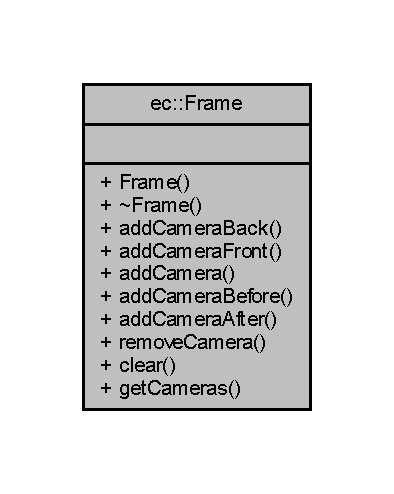
\includegraphics[width=189pt]{classec_1_1_frame__coll__graph}
\end{center}
\end{figure}
\subsection*{Public Member Functions}
\begin{DoxyCompactItemize}
\item 
\mbox{\hyperlink{classec_1_1_frame_a80ed1da85818f646b6b80fb6c8a6c2a6}{Frame}} ()
\item 
\mbox{\hyperlink{classec_1_1_frame_af2b2c733cacb47d99e460a2b75667eaa}{$\sim$\+Frame}} ()
\item 
void \mbox{\hyperlink{classec_1_1_frame_a1cfcb26e088e6f6b07103af8ac9d3bfa}{add\+Camera\+Back}} (\mbox{\hyperlink{classec_1_1_camera}{Camera}} $\ast$camera)
\item 
void \mbox{\hyperlink{classec_1_1_frame_abcbaa8a587c8ad75173aacaa853bc5b2}{add\+Camera\+Front}} (\mbox{\hyperlink{classec_1_1_camera}{Camera}} $\ast$camera)
\item 
void \mbox{\hyperlink{classec_1_1_frame_a04ba39407bc0f6e78fe47f37b3f19131}{add\+Camera}} (\mbox{\hyperlink{classec_1_1_camera}{Camera}} $\ast$camera, unsigned int priority)
\item 
bool \mbox{\hyperlink{classec_1_1_frame_af1f1769a61f70a756fd762d80a676063}{add\+Camera\+Before}} (\mbox{\hyperlink{classec_1_1_camera}{Camera}} $\ast$camera, \mbox{\hyperlink{classec_1_1_camera}{Camera}} $\ast$next\+Camera)
\item 
bool \mbox{\hyperlink{classec_1_1_frame_a60b34025921413dd3ea92c9146d76825}{add\+Camera\+After}} (\mbox{\hyperlink{classec_1_1_camera}{Camera}} $\ast$camera, \mbox{\hyperlink{classec_1_1_camera}{Camera}} $\ast$prev\+Camera)
\item 
bool \mbox{\hyperlink{classec_1_1_frame_a7a93ec89a809f5b7e685c5adc73d6cda}{remove\+Camera}} (\mbox{\hyperlink{classec_1_1_camera}{Camera}} $\ast$camera)
\item 
void \mbox{\hyperlink{classec_1_1_frame_ae9896c9acff0f468a750d9eae784b23b}{clear}} ()
\item 
std\+::vector$<$ \mbox{\hyperlink{classec_1_1_camera}{Camera}} $\ast$ $>$ \& \mbox{\hyperlink{classec_1_1_frame_a942b4c8826f6169703ff6b19ae60be8c}{get\+Cameras}} ()
\item 
const std\+::vector$<$ \mbox{\hyperlink{classec_1_1_camera}{Camera}} $\ast$ $>$ \& \mbox{\hyperlink{classec_1_1_frame_a80aefbcba8339fabc3b4aa2b8b21a8bf}{get\+Cameras}} () const
\end{DoxyCompactItemize}


\subsection{Detailed Description}
A \mbox{\hyperlink{classec_1_1_frame}{Frame}} is a collection of cameras. The order in, which these cameras are stored, determines the order in which will be rendered. 

\subsection{Constructor \& Destructor Documentation}
\mbox{\Hypertarget{classec_1_1_frame_a80ed1da85818f646b6b80fb6c8a6c2a6}\label{classec_1_1_frame_a80ed1da85818f646b6b80fb6c8a6c2a6}} 
\index{ec\+::\+Frame@{ec\+::\+Frame}!Frame@{Frame}}
\index{Frame@{Frame}!ec\+::\+Frame@{ec\+::\+Frame}}
\subsubsection{\texorpdfstring{Frame()}{Frame()}}
{\footnotesize\ttfamily ec\+::\+Frame\+::\+Frame (\begin{DoxyParamCaption}{ }\end{DoxyParamCaption})\hspace{0.3cm}{\ttfamily [explicit]}, {\ttfamily [default]}}

\mbox{\Hypertarget{classec_1_1_frame_af2b2c733cacb47d99e460a2b75667eaa}\label{classec_1_1_frame_af2b2c733cacb47d99e460a2b75667eaa}} 
\index{ec\+::\+Frame@{ec\+::\+Frame}!````~Frame@{$\sim$\+Frame}}
\index{````~Frame@{$\sim$\+Frame}!ec\+::\+Frame@{ec\+::\+Frame}}
\subsubsection{\texorpdfstring{$\sim$\+Frame()}{~Frame()}}
{\footnotesize\ttfamily ec\+::\+Frame\+::$\sim$\+Frame (\begin{DoxyParamCaption}{ }\end{DoxyParamCaption})\hspace{0.3cm}{\ttfamily [default]}}



\subsection{Member Function Documentation}
\mbox{\Hypertarget{classec_1_1_frame_a04ba39407bc0f6e78fe47f37b3f19131}\label{classec_1_1_frame_a04ba39407bc0f6e78fe47f37b3f19131}} 
\index{ec\+::\+Frame@{ec\+::\+Frame}!add\+Camera@{add\+Camera}}
\index{add\+Camera@{add\+Camera}!ec\+::\+Frame@{ec\+::\+Frame}}
\subsubsection{\texorpdfstring{add\+Camera()}{addCamera()}}
{\footnotesize\ttfamily void ec\+::\+Frame\+::add\+Camera (\begin{DoxyParamCaption}\item[{\mbox{\hyperlink{classec_1_1_camera}{Camera}} $\ast$}]{camera,  }\item[{unsigned int}]{priority }\end{DoxyParamCaption})}

Add a given camera with a given priority. If there already is a camera with the same priority registered, put the given camera before this. \mbox{\Hypertarget{classec_1_1_frame_a60b34025921413dd3ea92c9146d76825}\label{classec_1_1_frame_a60b34025921413dd3ea92c9146d76825}} 
\index{ec\+::\+Frame@{ec\+::\+Frame}!add\+Camera\+After@{add\+Camera\+After}}
\index{add\+Camera\+After@{add\+Camera\+After}!ec\+::\+Frame@{ec\+::\+Frame}}
\subsubsection{\texorpdfstring{add\+Camera\+After()}{addCameraAfter()}}
{\footnotesize\ttfamily bool ec\+::\+Frame\+::add\+Camera\+After (\begin{DoxyParamCaption}\item[{\mbox{\hyperlink{classec_1_1_camera}{Camera}} $\ast$}]{camera,  }\item[{\mbox{\hyperlink{classec_1_1_camera}{Camera}} $\ast$}]{prev\+Camera }\end{DoxyParamCaption})}

Add a given camera right after another given camera 
\begin{DoxyParams}{Parameters}
{\em camera} & The camera to be added. \\
\hline
{\em prev\+Camera} & The camera after which the newly added camera should follow. \\
\hline
\end{DoxyParams}
\begin{DoxyReturn}{Returns}
True if prev\+Camera was found, false otherwise. 
\end{DoxyReturn}
\mbox{\Hypertarget{classec_1_1_frame_a1cfcb26e088e6f6b07103af8ac9d3bfa}\label{classec_1_1_frame_a1cfcb26e088e6f6b07103af8ac9d3bfa}} 
\index{ec\+::\+Frame@{ec\+::\+Frame}!add\+Camera\+Back@{add\+Camera\+Back}}
\index{add\+Camera\+Back@{add\+Camera\+Back}!ec\+::\+Frame@{ec\+::\+Frame}}
\subsubsection{\texorpdfstring{add\+Camera\+Back()}{addCameraBack()}}
{\footnotesize\ttfamily void ec\+::\+Frame\+::add\+Camera\+Back (\begin{DoxyParamCaption}\item[{\mbox{\hyperlink{classec_1_1_camera}{Camera}} $\ast$}]{camera }\end{DoxyParamCaption})}

Add a given camera at the end (low priority camera) \mbox{\Hypertarget{classec_1_1_frame_af1f1769a61f70a756fd762d80a676063}\label{classec_1_1_frame_af1f1769a61f70a756fd762d80a676063}} 
\index{ec\+::\+Frame@{ec\+::\+Frame}!add\+Camera\+Before@{add\+Camera\+Before}}
\index{add\+Camera\+Before@{add\+Camera\+Before}!ec\+::\+Frame@{ec\+::\+Frame}}
\subsubsection{\texorpdfstring{add\+Camera\+Before()}{addCameraBefore()}}
{\footnotesize\ttfamily bool ec\+::\+Frame\+::add\+Camera\+Before (\begin{DoxyParamCaption}\item[{\mbox{\hyperlink{classec_1_1_camera}{Camera}} $\ast$}]{camera,  }\item[{\mbox{\hyperlink{classec_1_1_camera}{Camera}} $\ast$}]{next\+Camera }\end{DoxyParamCaption})}

Add a given camera right before another given camera 
\begin{DoxyParams}{Parameters}
{\em camera} & The camera to be added. \\
\hline
{\em next\+Camera} & The camera before which the newly added camera should follow. \\
\hline
\end{DoxyParams}
\begin{DoxyReturn}{Returns}
True if next\+Camera was found, false otherwise. 
\end{DoxyReturn}
\mbox{\Hypertarget{classec_1_1_frame_abcbaa8a587c8ad75173aacaa853bc5b2}\label{classec_1_1_frame_abcbaa8a587c8ad75173aacaa853bc5b2}} 
\index{ec\+::\+Frame@{ec\+::\+Frame}!add\+Camera\+Front@{add\+Camera\+Front}}
\index{add\+Camera\+Front@{add\+Camera\+Front}!ec\+::\+Frame@{ec\+::\+Frame}}
\subsubsection{\texorpdfstring{add\+Camera\+Front()}{addCameraFront()}}
{\footnotesize\ttfamily void ec\+::\+Frame\+::add\+Camera\+Front (\begin{DoxyParamCaption}\item[{\mbox{\hyperlink{classec_1_1_camera}{Camera}} $\ast$}]{camera }\end{DoxyParamCaption})}

Add a given camera at the front (high priority camera) \mbox{\Hypertarget{classec_1_1_frame_ae9896c9acff0f468a750d9eae784b23b}\label{classec_1_1_frame_ae9896c9acff0f468a750d9eae784b23b}} 
\index{ec\+::\+Frame@{ec\+::\+Frame}!clear@{clear}}
\index{clear@{clear}!ec\+::\+Frame@{ec\+::\+Frame}}
\subsubsection{\texorpdfstring{clear()}{clear()}}
{\footnotesize\ttfamily void ec\+::\+Frame\+::clear (\begin{DoxyParamCaption}{ }\end{DoxyParamCaption})}

Remove all registered cameras. \mbox{\Hypertarget{classec_1_1_frame_a942b4c8826f6169703ff6b19ae60be8c}\label{classec_1_1_frame_a942b4c8826f6169703ff6b19ae60be8c}} 
\index{ec\+::\+Frame@{ec\+::\+Frame}!get\+Cameras@{get\+Cameras}}
\index{get\+Cameras@{get\+Cameras}!ec\+::\+Frame@{ec\+::\+Frame}}
\subsubsection{\texorpdfstring{get\+Cameras()}{getCameras()}\hspace{0.1cm}{\footnotesize\ttfamily [1/2]}}
{\footnotesize\ttfamily std\+::vector$<$ \mbox{\hyperlink{classec_1_1_camera}{Camera}} $\ast$ $>$ \& ec\+::\+Frame\+::get\+Cameras (\begin{DoxyParamCaption}{ }\end{DoxyParamCaption})}

Get all registered cameras \mbox{\Hypertarget{classec_1_1_frame_a80aefbcba8339fabc3b4aa2b8b21a8bf}\label{classec_1_1_frame_a80aefbcba8339fabc3b4aa2b8b21a8bf}} 
\index{ec\+::\+Frame@{ec\+::\+Frame}!get\+Cameras@{get\+Cameras}}
\index{get\+Cameras@{get\+Cameras}!ec\+::\+Frame@{ec\+::\+Frame}}
\subsubsection{\texorpdfstring{get\+Cameras()}{getCameras()}\hspace{0.1cm}{\footnotesize\ttfamily [2/2]}}
{\footnotesize\ttfamily const std\+::vector$<$ \mbox{\hyperlink{classec_1_1_camera}{Camera}} $\ast$ $>$ \& ec\+::\+Frame\+::get\+Cameras (\begin{DoxyParamCaption}{ }\end{DoxyParamCaption}) const}

Get all registered cameras \mbox{\Hypertarget{classec_1_1_frame_a7a93ec89a809f5b7e685c5adc73d6cda}\label{classec_1_1_frame_a7a93ec89a809f5b7e685c5adc73d6cda}} 
\index{ec\+::\+Frame@{ec\+::\+Frame}!remove\+Camera@{remove\+Camera}}
\index{remove\+Camera@{remove\+Camera}!ec\+::\+Frame@{ec\+::\+Frame}}
\subsubsection{\texorpdfstring{remove\+Camera()}{removeCamera()}}
{\footnotesize\ttfamily bool ec\+::\+Frame\+::remove\+Camera (\begin{DoxyParamCaption}\item[{\mbox{\hyperlink{classec_1_1_camera}{Camera}} $\ast$}]{camera }\end{DoxyParamCaption})}

Remove a given camera from the frame. 
\begin{DoxyParams}{Parameters}
{\em camera} & The camera to be removed. \\
\hline
\end{DoxyParams}
\begin{DoxyReturn}{Returns}
True if the given camera is registered, false otherwise. 
\end{DoxyReturn}


The documentation for this class was generated from the following files\+:\begin{DoxyCompactItemize}
\item 
C\+:/\+Library/\+Job/\+Projekte/\+Simulation\+Visualization/\+Eye\+Candy3\+D/\+Eye\+Candy3\+D/include/\+E\+C3\+D/\+Core/\mbox{\hyperlink{_frame_8h}{Frame.\+h}}\item 
C\+:/\+Library/\+Job/\+Projekte/\+Simulation\+Visualization/\+Eye\+Candy3\+D/\+Eye\+Candy3\+D/src/\+Core/\mbox{\hyperlink{_frame_8cpp}{Frame.\+cpp}}\end{DoxyCompactItemize}

\hypertarget{classec_1_1_freetype}{}\section{ec\+:\+:Freetype Class Reference}
\label{classec_1_1_freetype}\index{ec\+::\+Freetype@{ec\+::\+Freetype}}


{\ttfamily \#include $<$Freetype.\+h$>$}



Collaboration diagram for ec\+:\+:Freetype\+:\nopagebreak
\begin{figure}[H]
\begin{center}
\leavevmode
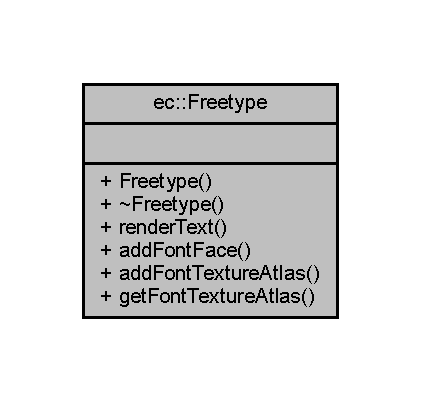
\includegraphics[width=202pt]{classec_1_1_freetype__coll__graph}
\end{center}
\end{figure}
\subsection*{Public Member Functions}
\begin{DoxyCompactItemize}
\item 
\mbox{\hyperlink{classec_1_1_freetype_a77da5cdd8b053a5fea7c5ffd78c39418}{Freetype}} (\mbox{\hyperlink{classec_1_1_shader}{Shader}} $\ast$shader)
\item 
\mbox{\hyperlink{classec_1_1_freetype_a35e8fad09705600cdd263ed3781d299b}{$\sim$\+Freetype}} ()
\item 
void \mbox{\hyperlink{classec_1_1_freetype_afef1f61fa4bd8114825c66ac93d3e6bf}{render\+Text}} (const char $\ast$\mbox{\hyperlink{namespaceec_a5de6bdb8c4b2ed6e590e721ec998f964a1cb251ec0d568de6a929b520c4aed8d1}{text}}, \mbox{\hyperlink{classec_1_1_font_texture_atlas}{Font\+Texture\+Atlas}} $\ast$atlas, float x, float y, float sx, float sy, const glm\+::vec4 \&color=glm\+::vec4(0.\+0f, 0.\+0f, 0.\+0f, 1.\+0f)) const
\item 
void \mbox{\hyperlink{classec_1_1_freetype_a7a10e5515342b70588f76328ac83826d}{add\+Font\+Face}} (const std\+::string \&name, const std\+::string \&filepath)
\item 
void \mbox{\hyperlink{classec_1_1_freetype_a1be4b69e2d57689533ddaabdc9042d51}{add\+Font\+Texture\+Atlas}} (const std\+::string \&face, unsigned int size)
\item 
\mbox{\hyperlink{classec_1_1_font_texture_atlas}{Font\+Texture\+Atlas}} $\ast$ \mbox{\hyperlink{classec_1_1_freetype_a3e0a8937ec0ceb33495598da59b2c4f3}{get\+Font\+Texture\+Atlas}} (const std\+::string \&name)
\end{DoxyCompactItemize}


\subsection{Constructor \& Destructor Documentation}
\mbox{\Hypertarget{classec_1_1_freetype_a77da5cdd8b053a5fea7c5ffd78c39418}\label{classec_1_1_freetype_a77da5cdd8b053a5fea7c5ffd78c39418}} 
\index{ec\+::\+Freetype@{ec\+::\+Freetype}!Freetype@{Freetype}}
\index{Freetype@{Freetype}!ec\+::\+Freetype@{ec\+::\+Freetype}}
\subsubsection{\texorpdfstring{Freetype()}{Freetype()}}
{\footnotesize\ttfamily ec\+::\+Freetype\+::\+Freetype (\begin{DoxyParamCaption}\item[{\mbox{\hyperlink{classec_1_1_shader}{Shader}} $\ast$}]{shader }\end{DoxyParamCaption})\hspace{0.3cm}{\ttfamily [explicit]}}

\mbox{\Hypertarget{classec_1_1_freetype_a35e8fad09705600cdd263ed3781d299b}\label{classec_1_1_freetype_a35e8fad09705600cdd263ed3781d299b}} 
\index{ec\+::\+Freetype@{ec\+::\+Freetype}!````~Freetype@{$\sim$\+Freetype}}
\index{````~Freetype@{$\sim$\+Freetype}!ec\+::\+Freetype@{ec\+::\+Freetype}}
\subsubsection{\texorpdfstring{$\sim$\+Freetype()}{~Freetype()}}
{\footnotesize\ttfamily ec\+::\+Freetype\+::$\sim$\+Freetype (\begin{DoxyParamCaption}{ }\end{DoxyParamCaption})\hspace{0.3cm}{\ttfamily [default]}}



\subsection{Member Function Documentation}
\mbox{\Hypertarget{classec_1_1_freetype_a7a10e5515342b70588f76328ac83826d}\label{classec_1_1_freetype_a7a10e5515342b70588f76328ac83826d}} 
\index{ec\+::\+Freetype@{ec\+::\+Freetype}!add\+Font\+Face@{add\+Font\+Face}}
\index{add\+Font\+Face@{add\+Font\+Face}!ec\+::\+Freetype@{ec\+::\+Freetype}}
\subsubsection{\texorpdfstring{add\+Font\+Face()}{addFontFace()}}
{\footnotesize\ttfamily void ec\+::\+Freetype\+::add\+Font\+Face (\begin{DoxyParamCaption}\item[{const std\+::string \&}]{name,  }\item[{const std\+::string \&}]{filepath }\end{DoxyParamCaption})}

\mbox{\Hypertarget{classec_1_1_freetype_a1be4b69e2d57689533ddaabdc9042d51}\label{classec_1_1_freetype_a1be4b69e2d57689533ddaabdc9042d51}} 
\index{ec\+::\+Freetype@{ec\+::\+Freetype}!add\+Font\+Texture\+Atlas@{add\+Font\+Texture\+Atlas}}
\index{add\+Font\+Texture\+Atlas@{add\+Font\+Texture\+Atlas}!ec\+::\+Freetype@{ec\+::\+Freetype}}
\subsubsection{\texorpdfstring{add\+Font\+Texture\+Atlas()}{addFontTextureAtlas()}}
{\footnotesize\ttfamily void ec\+::\+Freetype\+::add\+Font\+Texture\+Atlas (\begin{DoxyParamCaption}\item[{const std\+::string \&}]{face,  }\item[{unsigned int}]{size }\end{DoxyParamCaption})}

\mbox{\Hypertarget{classec_1_1_freetype_a3e0a8937ec0ceb33495598da59b2c4f3}\label{classec_1_1_freetype_a3e0a8937ec0ceb33495598da59b2c4f3}} 
\index{ec\+::\+Freetype@{ec\+::\+Freetype}!get\+Font\+Texture\+Atlas@{get\+Font\+Texture\+Atlas}}
\index{get\+Font\+Texture\+Atlas@{get\+Font\+Texture\+Atlas}!ec\+::\+Freetype@{ec\+::\+Freetype}}
\subsubsection{\texorpdfstring{get\+Font\+Texture\+Atlas()}{getFontTextureAtlas()}}
{\footnotesize\ttfamily \mbox{\hyperlink{classec_1_1_font_texture_atlas}{Font\+Texture\+Atlas}} $\ast$ ec\+::\+Freetype\+::get\+Font\+Texture\+Atlas (\begin{DoxyParamCaption}\item[{const std\+::string \&}]{name }\end{DoxyParamCaption})}

\mbox{\Hypertarget{classec_1_1_freetype_afef1f61fa4bd8114825c66ac93d3e6bf}\label{classec_1_1_freetype_afef1f61fa4bd8114825c66ac93d3e6bf}} 
\index{ec\+::\+Freetype@{ec\+::\+Freetype}!render\+Text@{render\+Text}}
\index{render\+Text@{render\+Text}!ec\+::\+Freetype@{ec\+::\+Freetype}}
\subsubsection{\texorpdfstring{render\+Text()}{renderText()}}
{\footnotesize\ttfamily void ec\+::\+Freetype\+::render\+Text (\begin{DoxyParamCaption}\item[{const char $\ast$}]{text,  }\item[{\mbox{\hyperlink{classec_1_1_font_texture_atlas}{Font\+Texture\+Atlas}} $\ast$}]{atlas,  }\item[{float}]{x,  }\item[{float}]{y,  }\item[{float}]{sx,  }\item[{float}]{sy,  }\item[{const glm\+::vec4 \&}]{color = {\ttfamily glm\+:\+:vec4(0.0f,~0.0f,~0.0f,~1.0f)} }\end{DoxyParamCaption}) const}



The documentation for this class was generated from the following files\+:\begin{DoxyCompactItemize}
\item 
D\+:/\+Library/\+Documents/\+Job/\+Forschungsmaster/\+Projekte/\+Eye\+Candy3\+D/\+Eye\+Candy3\+D/include/\+E\+C3\+D/\+Core/\mbox{\hyperlink{_freetype_8h}{Freetype.\+h}}\item 
D\+:/\+Library/\+Documents/\+Job/\+Forschungsmaster/\+Projekte/\+Eye\+Candy3\+D/\+Eye\+Candy3\+D/src/\+Core/\mbox{\hyperlink{_freetype_8cpp}{Freetype.\+cpp}}\end{DoxyCompactItemize}

\hypertarget{classec_1_1_geometry}{}\section{ec\+:\+:Geometry Class Reference}
\label{classec_1_1_geometry}\index{ec\+::\+Geometry@{ec\+::\+Geometry}}


{\ttfamily \#include $<$Geometry.\+h$>$}



Inheritance diagram for ec\+:\+:Geometry\+:\nopagebreak
\begin{figure}[H]
\begin{center}
\leavevmode
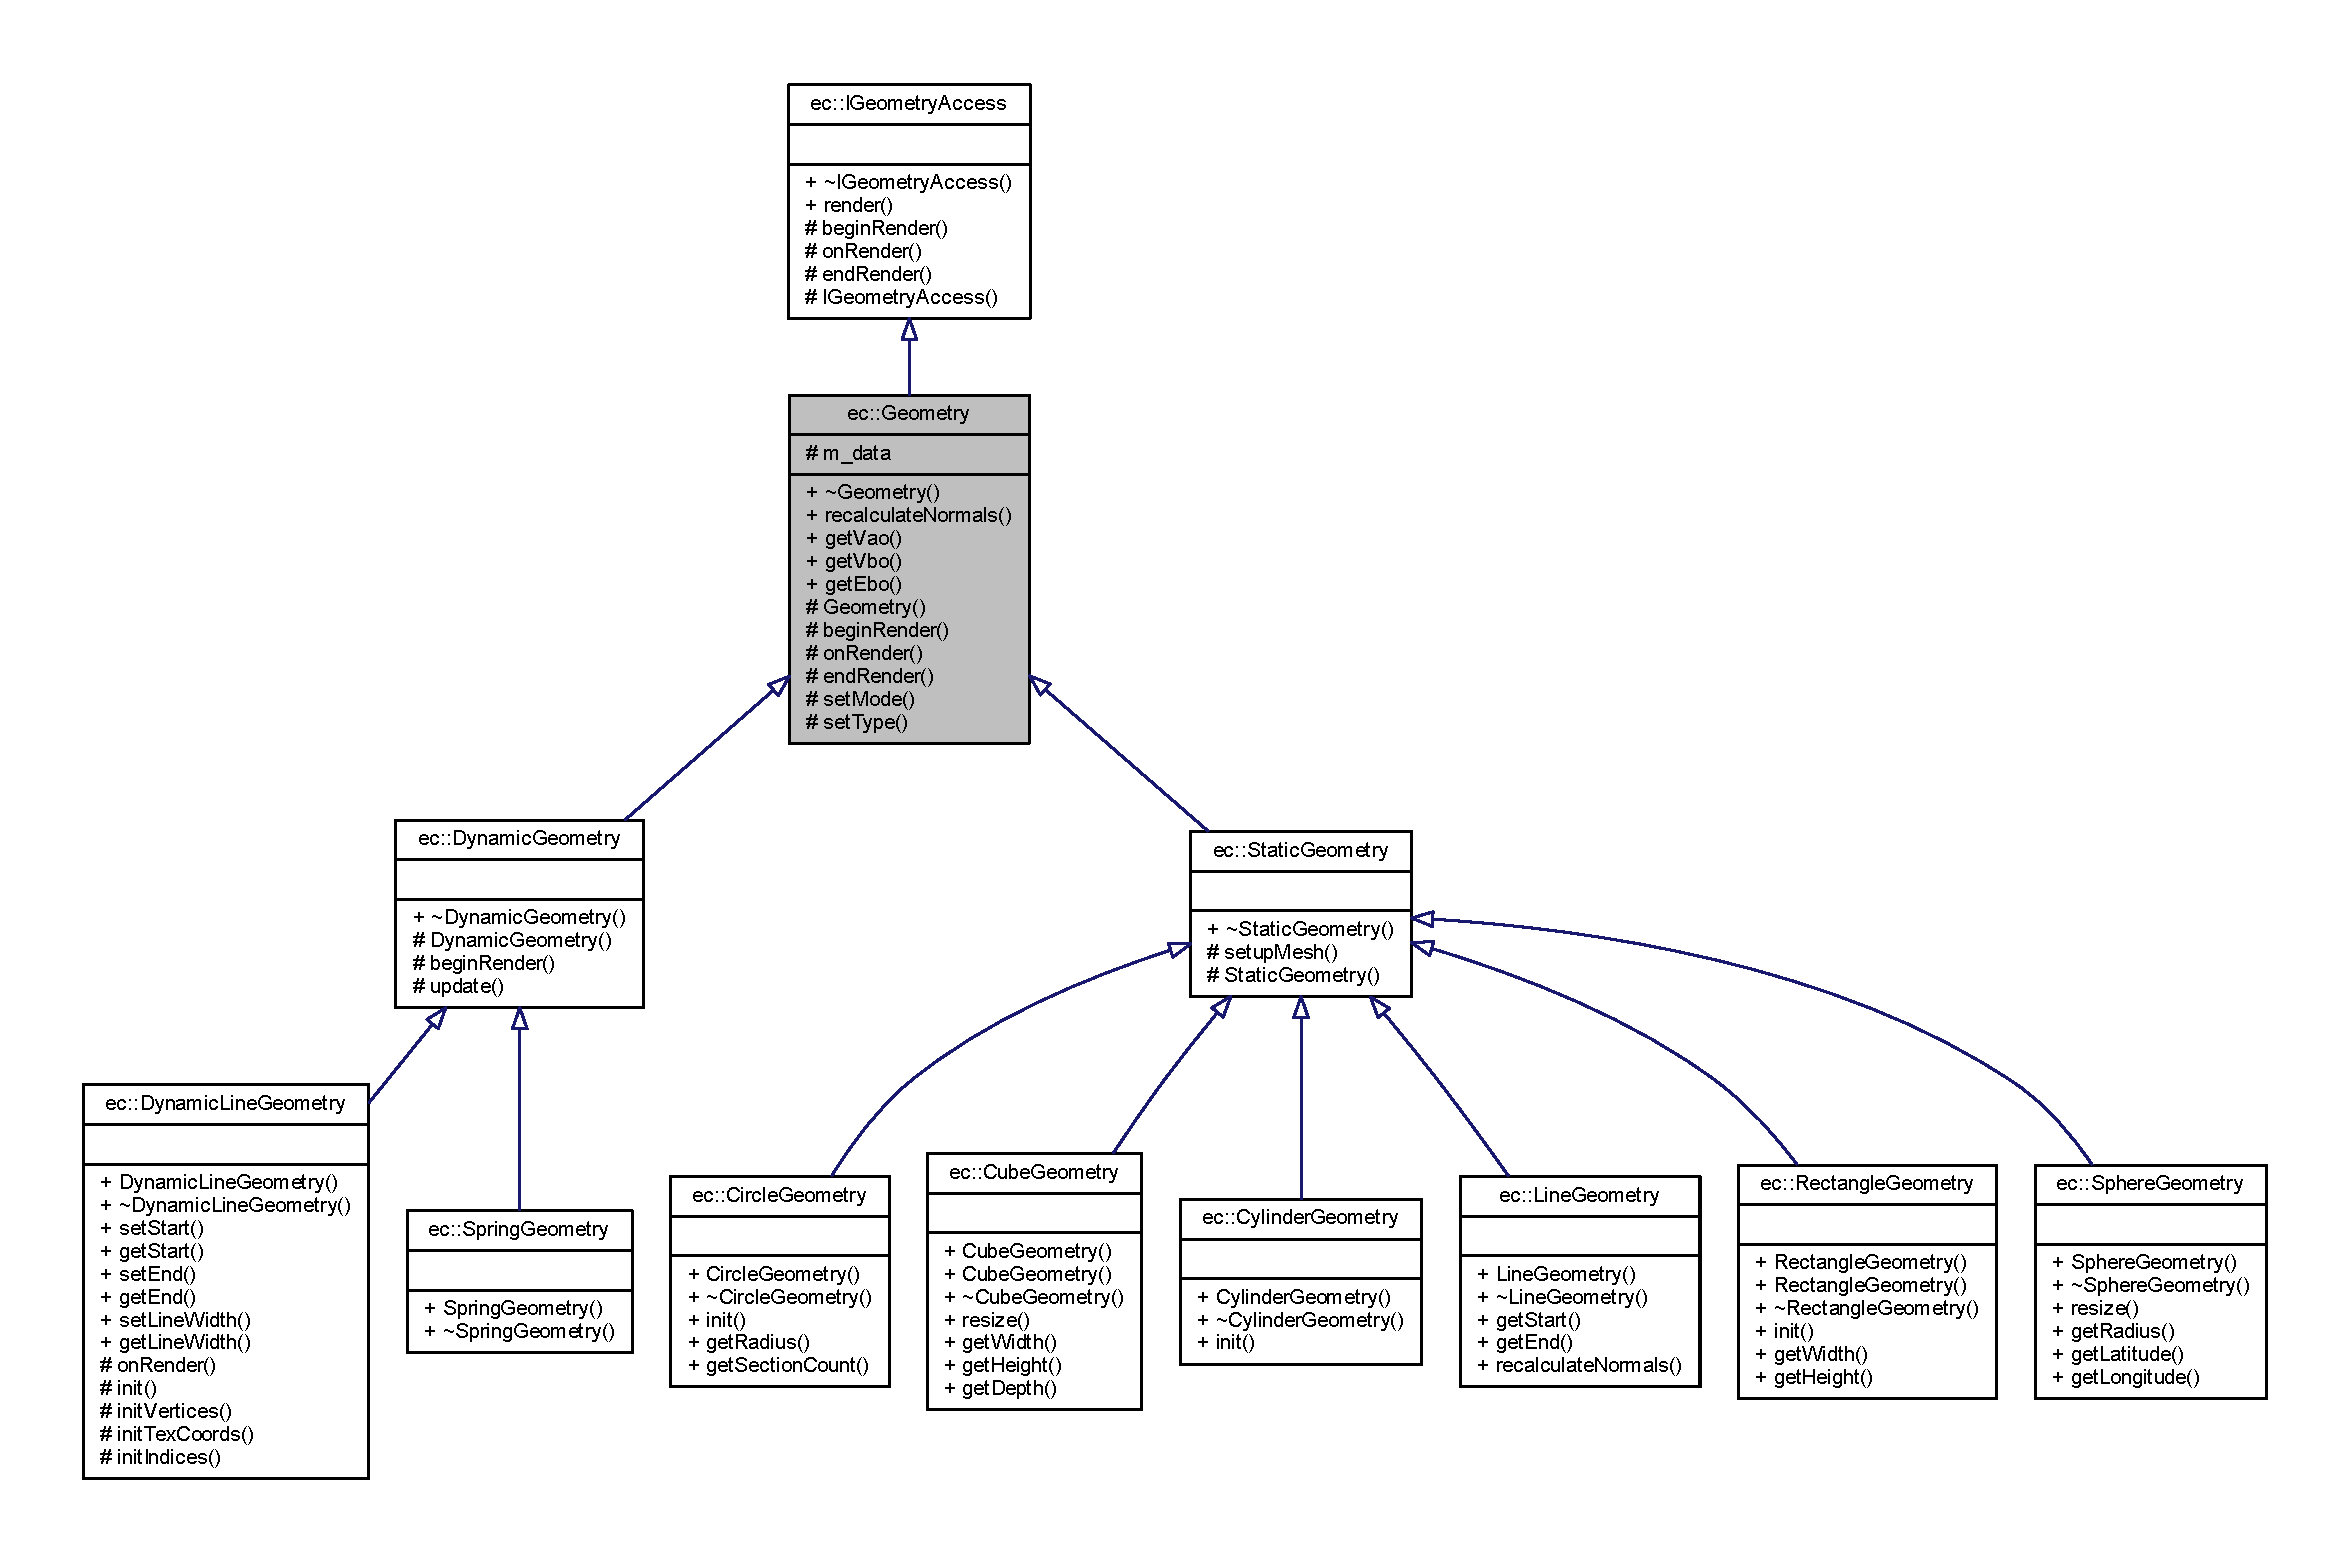
\includegraphics[width=350pt]{classec_1_1_geometry__inherit__graph}
\end{center}
\end{figure}


Collaboration diagram for ec\+:\+:Geometry\+:\nopagebreak
\begin{figure}[H]
\begin{center}
\leavevmode
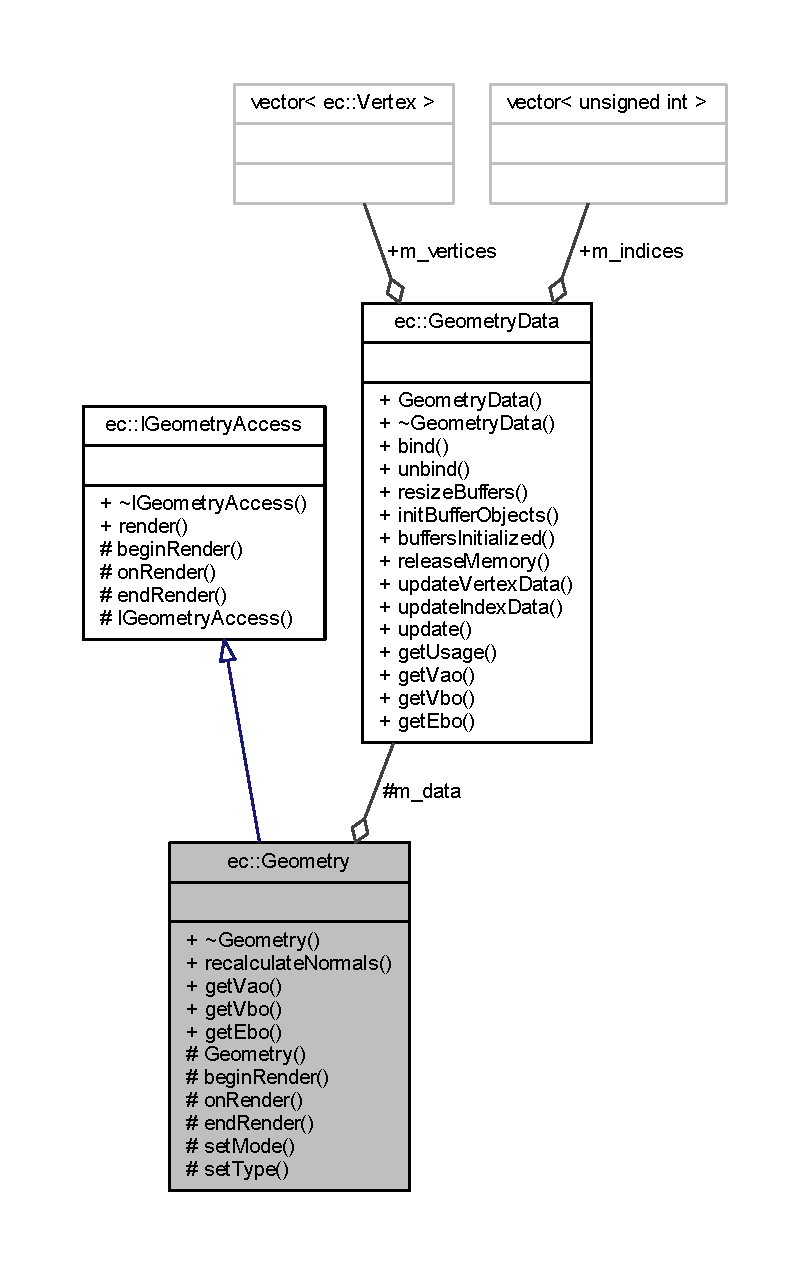
\includegraphics[width=350pt]{classec_1_1_geometry__coll__graph}
\end{center}
\end{figure}
\subsection*{Public Member Functions}
\begin{DoxyCompactItemize}
\item 
virtual \mbox{\hyperlink{classec_1_1_geometry_a964c581313da2be51a3c78d3be7f48b3}{$\sim$\+Geometry}} ()
\item 
virtual void \mbox{\hyperlink{classec_1_1_geometry_a228d4a0fa01a17379f24aee2c769b501}{recalculate\+Normals}} ()
\item 
G\+Luint \mbox{\hyperlink{classec_1_1_geometry_a91a89baad39d4f2b2c4e9774d952dce9}{get\+Vao}} () const
\item 
G\+Luint \mbox{\hyperlink{classec_1_1_geometry_abad5d4311d16462099b8f9d084d99dd4}{get\+Vbo}} () const
\item 
G\+Luint \mbox{\hyperlink{classec_1_1_geometry_a5d956ff01a7b6648ede8982e0a461ae0}{get\+Ebo}} () const
\end{DoxyCompactItemize}
\subsection*{Protected Member Functions}
\begin{DoxyCompactItemize}
\item 
\mbox{\hyperlink{classec_1_1_geometry_aeae22c6b54c7c534249ee08b3fb77a70}{Geometry}} (G\+Lenum mode=G\+L\+\_\+\+T\+R\+I\+A\+N\+G\+L\+ES, G\+Lenum type=G\+L\+\_\+\+U\+N\+S\+I\+G\+N\+E\+D\+\_\+\+I\+NT)
\item 
void \mbox{\hyperlink{classec_1_1_geometry_aeca5f0e52e7c2e4b352ede1a6e7c3f5b}{begin\+Render}} () override
\item 
void \mbox{\hyperlink{classec_1_1_geometry_a1f166e70fc880e88092f29ef46afb836}{on\+Render}} () override
\item 
void \mbox{\hyperlink{classec_1_1_geometry_ae0352702162501df185517e84c3b02bd}{end\+Render}} () override
\item 
void \mbox{\hyperlink{classec_1_1_geometry_ad4f80cd4d4c22b108c33b9030e91467b}{set\+Mode}} (G\+Lenum mode)
\item 
void \mbox{\hyperlink{classec_1_1_geometry_a12c3da280ff11e86a8b07d18a23e0880}{set\+Type}} (G\+Lenum type)
\end{DoxyCompactItemize}
\subsection*{Protected Attributes}
\begin{DoxyCompactItemize}
\item 
\mbox{\hyperlink{structec_1_1_geometry_data}{Geometry\+Data}} \mbox{\hyperlink{classec_1_1_geometry_aeb72a472b242d92496f0283cfee17fac}{m\+\_\+data}}
\end{DoxyCompactItemize}


\subsection{Constructor \& Destructor Documentation}
\mbox{\Hypertarget{classec_1_1_geometry_a964c581313da2be51a3c78d3be7f48b3}\label{classec_1_1_geometry_a964c581313da2be51a3c78d3be7f48b3}} 
\index{ec\+::\+Geometry@{ec\+::\+Geometry}!````~Geometry@{$\sim$\+Geometry}}
\index{````~Geometry@{$\sim$\+Geometry}!ec\+::\+Geometry@{ec\+::\+Geometry}}
\subsubsection{\texorpdfstring{$\sim$\+Geometry()}{~Geometry()}}
{\footnotesize\ttfamily ec\+::\+Geometry\+::$\sim$\+Geometry (\begin{DoxyParamCaption}{ }\end{DoxyParamCaption})\hspace{0.3cm}{\ttfamily [virtual]}, {\ttfamily [default]}}

\mbox{\Hypertarget{classec_1_1_geometry_aeae22c6b54c7c534249ee08b3fb77a70}\label{classec_1_1_geometry_aeae22c6b54c7c534249ee08b3fb77a70}} 
\index{ec\+::\+Geometry@{ec\+::\+Geometry}!Geometry@{Geometry}}
\index{Geometry@{Geometry}!ec\+::\+Geometry@{ec\+::\+Geometry}}
\subsubsection{\texorpdfstring{Geometry()}{Geometry()}}
{\footnotesize\ttfamily ec\+::\+Geometry\+::\+Geometry (\begin{DoxyParamCaption}\item[{G\+Lenum}]{mode = {\ttfamily GL\+\_\+TRIANGLES},  }\item[{G\+Lenum}]{type = {\ttfamily GL\+\_\+UNSIGNED\+\_\+INT} }\end{DoxyParamCaption})\hspace{0.3cm}{\ttfamily [explicit]}, {\ttfamily [protected]}}



\subsection{Member Function Documentation}
\mbox{\Hypertarget{classec_1_1_geometry_aeca5f0e52e7c2e4b352ede1a6e7c3f5b}\label{classec_1_1_geometry_aeca5f0e52e7c2e4b352ede1a6e7c3f5b}} 
\index{ec\+::\+Geometry@{ec\+::\+Geometry}!begin\+Render@{begin\+Render}}
\index{begin\+Render@{begin\+Render}!ec\+::\+Geometry@{ec\+::\+Geometry}}
\subsubsection{\texorpdfstring{begin\+Render()}{beginRender()}}
{\footnotesize\ttfamily void ec\+::\+Geometry\+::begin\+Render (\begin{DoxyParamCaption}{ }\end{DoxyParamCaption})\hspace{0.3cm}{\ttfamily [override]}, {\ttfamily [protected]}, {\ttfamily [virtual]}}

Called at the beginning of the rendering routine. 

Implements \mbox{\hyperlink{classec_1_1_i_geometry_access_a17a87aca44e2a23a6185e78262e02652}{ec\+::\+I\+Geometry\+Access}}.

\mbox{\Hypertarget{classec_1_1_geometry_ae0352702162501df185517e84c3b02bd}\label{classec_1_1_geometry_ae0352702162501df185517e84c3b02bd}} 
\index{ec\+::\+Geometry@{ec\+::\+Geometry}!end\+Render@{end\+Render}}
\index{end\+Render@{end\+Render}!ec\+::\+Geometry@{ec\+::\+Geometry}}
\subsubsection{\texorpdfstring{end\+Render()}{endRender()}}
{\footnotesize\ttfamily void ec\+::\+Geometry\+::end\+Render (\begin{DoxyParamCaption}{ }\end{DoxyParamCaption})\hspace{0.3cm}{\ttfamily [override]}, {\ttfamily [protected]}, {\ttfamily [virtual]}}

Called at the end of the rendering routine. 

Implements \mbox{\hyperlink{classec_1_1_i_geometry_access_a6d3b9c34a8b73aeac26663ef349ce41f}{ec\+::\+I\+Geometry\+Access}}.

\mbox{\Hypertarget{classec_1_1_geometry_a5d956ff01a7b6648ede8982e0a461ae0}\label{classec_1_1_geometry_a5d956ff01a7b6648ede8982e0a461ae0}} 
\index{ec\+::\+Geometry@{ec\+::\+Geometry}!get\+Ebo@{get\+Ebo}}
\index{get\+Ebo@{get\+Ebo}!ec\+::\+Geometry@{ec\+::\+Geometry}}
\subsubsection{\texorpdfstring{get\+Ebo()}{getEbo()}}
{\footnotesize\ttfamily G\+Luint ec\+::\+Geometry\+::get\+Ebo (\begin{DoxyParamCaption}{ }\end{DoxyParamCaption}) const}

Get the element buffer object id. \mbox{\Hypertarget{classec_1_1_geometry_a91a89baad39d4f2b2c4e9774d952dce9}\label{classec_1_1_geometry_a91a89baad39d4f2b2c4e9774d952dce9}} 
\index{ec\+::\+Geometry@{ec\+::\+Geometry}!get\+Vao@{get\+Vao}}
\index{get\+Vao@{get\+Vao}!ec\+::\+Geometry@{ec\+::\+Geometry}}
\subsubsection{\texorpdfstring{get\+Vao()}{getVao()}}
{\footnotesize\ttfamily G\+Luint ec\+::\+Geometry\+::get\+Vao (\begin{DoxyParamCaption}{ }\end{DoxyParamCaption}) const}

Get the vertex array object id. \mbox{\Hypertarget{classec_1_1_geometry_abad5d4311d16462099b8f9d084d99dd4}\label{classec_1_1_geometry_abad5d4311d16462099b8f9d084d99dd4}} 
\index{ec\+::\+Geometry@{ec\+::\+Geometry}!get\+Vbo@{get\+Vbo}}
\index{get\+Vbo@{get\+Vbo}!ec\+::\+Geometry@{ec\+::\+Geometry}}
\subsubsection{\texorpdfstring{get\+Vbo()}{getVbo()}}
{\footnotesize\ttfamily G\+Luint ec\+::\+Geometry\+::get\+Vbo (\begin{DoxyParamCaption}{ }\end{DoxyParamCaption}) const}

Get the vertex buffer object id. \mbox{\Hypertarget{classec_1_1_geometry_a1f166e70fc880e88092f29ef46afb836}\label{classec_1_1_geometry_a1f166e70fc880e88092f29ef46afb836}} 
\index{ec\+::\+Geometry@{ec\+::\+Geometry}!on\+Render@{on\+Render}}
\index{on\+Render@{on\+Render}!ec\+::\+Geometry@{ec\+::\+Geometry}}
\subsubsection{\texorpdfstring{on\+Render()}{onRender()}}
{\footnotesize\ttfamily void ec\+::\+Geometry\+::on\+Render (\begin{DoxyParamCaption}{ }\end{DoxyParamCaption})\hspace{0.3cm}{\ttfamily [override]}, {\ttfamily [protected]}, {\ttfamily [virtual]}}

The actual rendering of the object. 

Implements \mbox{\hyperlink{classec_1_1_i_geometry_access_a2ee418c9fa4eb266347bae2f0ef8095b}{ec\+::\+I\+Geometry\+Access}}.

\mbox{\Hypertarget{classec_1_1_geometry_a228d4a0fa01a17379f24aee2c769b501}\label{classec_1_1_geometry_a228d4a0fa01a17379f24aee2c769b501}} 
\index{ec\+::\+Geometry@{ec\+::\+Geometry}!recalculate\+Normals@{recalculate\+Normals}}
\index{recalculate\+Normals@{recalculate\+Normals}!ec\+::\+Geometry@{ec\+::\+Geometry}}
\subsubsection{\texorpdfstring{recalculate\+Normals()}{recalculateNormals()}}
{\footnotesize\ttfamily void ec\+::\+Geometry\+::recalculate\+Normals (\begin{DoxyParamCaption}{ }\end{DoxyParamCaption})\hspace{0.3cm}{\ttfamily [virtual]}}

Recalculate vertex normals. \mbox{\Hypertarget{classec_1_1_geometry_ad4f80cd4d4c22b108c33b9030e91467b}\label{classec_1_1_geometry_ad4f80cd4d4c22b108c33b9030e91467b}} 
\index{ec\+::\+Geometry@{ec\+::\+Geometry}!set\+Mode@{set\+Mode}}
\index{set\+Mode@{set\+Mode}!ec\+::\+Geometry@{ec\+::\+Geometry}}
\subsubsection{\texorpdfstring{set\+Mode()}{setMode()}}
{\footnotesize\ttfamily void ec\+::\+Geometry\+::set\+Mode (\begin{DoxyParamCaption}\item[{G\+Lenum}]{mode }\end{DoxyParamCaption})\hspace{0.3cm}{\ttfamily [protected]}}

\mbox{\Hypertarget{classec_1_1_geometry_a12c3da280ff11e86a8b07d18a23e0880}\label{classec_1_1_geometry_a12c3da280ff11e86a8b07d18a23e0880}} 
\index{ec\+::\+Geometry@{ec\+::\+Geometry}!set\+Type@{set\+Type}}
\index{set\+Type@{set\+Type}!ec\+::\+Geometry@{ec\+::\+Geometry}}
\subsubsection{\texorpdfstring{set\+Type()}{setType()}}
{\footnotesize\ttfamily void ec\+::\+Geometry\+::set\+Type (\begin{DoxyParamCaption}\item[{G\+Lenum}]{type }\end{DoxyParamCaption})\hspace{0.3cm}{\ttfamily [protected]}}



\subsection{Member Data Documentation}
\mbox{\Hypertarget{classec_1_1_geometry_aeb72a472b242d92496f0283cfee17fac}\label{classec_1_1_geometry_aeb72a472b242d92496f0283cfee17fac}} 
\index{ec\+::\+Geometry@{ec\+::\+Geometry}!m\+\_\+data@{m\+\_\+data}}
\index{m\+\_\+data@{m\+\_\+data}!ec\+::\+Geometry@{ec\+::\+Geometry}}
\subsubsection{\texorpdfstring{m\+\_\+data}{m\_data}}
{\footnotesize\ttfamily \mbox{\hyperlink{structec_1_1_geometry_data}{Geometry\+Data}} ec\+::\+Geometry\+::m\+\_\+data\hspace{0.3cm}{\ttfamily [protected]}}



The documentation for this class was generated from the following files\+:\begin{DoxyCompactItemize}
\item 
D\+:/\+Library/\+Documents/\+Job/\+Forschungsmaster/\+Projekte/\+Eye\+Candy3\+D/\+Eye\+Candy3\+D/include/\+E\+C3\+D/\+Core/\mbox{\hyperlink{_geometry_8h}{Geometry.\+h}}\item 
D\+:/\+Library/\+Documents/\+Job/\+Forschungsmaster/\+Projekte/\+Eye\+Candy3\+D/\+Eye\+Candy3\+D/src/\+Core/\mbox{\hyperlink{_geometry_8cpp}{Geometry.\+cpp}}\end{DoxyCompactItemize}

\hypertarget{classngl__gui_1_1_g_u_i}{}\section{ngl\+\_\+gui\+:\+:G\+UI Class Reference}
\label{classngl__gui_1_1_g_u_i}\index{ngl\+\_\+gui\+::\+G\+UI@{ngl\+\_\+gui\+::\+G\+UI}}


{\ttfamily \#include $<$G\+U\+I.\+h$>$}



Collaboration diagram for ngl\+\_\+gui\+:\+:G\+UI\+:\nopagebreak
\begin{figure}[H]
\begin{center}
\leavevmode
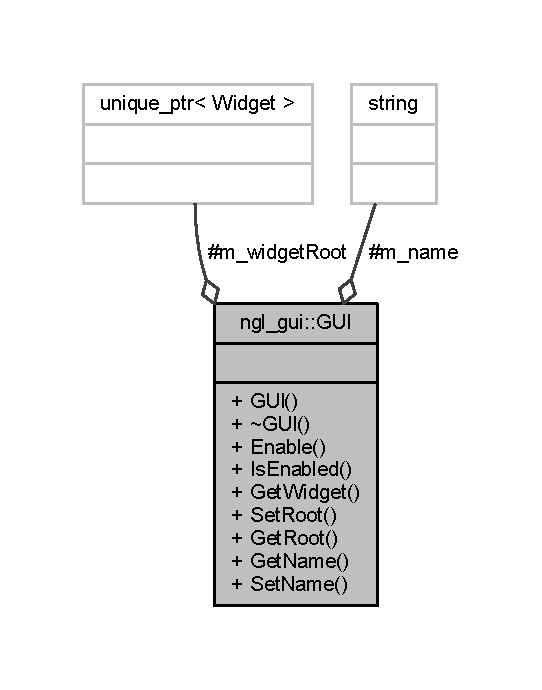
\includegraphics[width=260pt]{classngl__gui_1_1_g_u_i__coll__graph}
\end{center}
\end{figure}
\subsection*{Public Types}
\begin{DoxyCompactItemize}
\item 
using \mbox{\hyperlink{classngl__gui_1_1_g_u_i_af4d527c3697ea8524c7af82bb855286d}{Widget\+\_\+\+TP}} = std\+::unique\+\_\+ptr$<$ \mbox{\hyperlink{classngl__gui_1_1_widget}{Widget}} $>$
\end{DoxyCompactItemize}
\subsection*{Public Member Functions}
\begin{DoxyCompactItemize}
\item 
\mbox{\hyperlink{classngl__gui_1_1_g_u_i_a0b0002b02bdbf5fe660df18e104d96a8}{G\+UI}} (const std\+::string \&gui\+Name)
\item 
virtual \mbox{\hyperlink{classngl__gui_1_1_g_u_i_a1589c8616cbc59c64861bdbbcbb417b4}{$\sim$\+G\+UI}} ()
\item 
void \mbox{\hyperlink{classngl__gui_1_1_g_u_i_aa7dd88efa3541dd071aa80d7563bfc18}{Enable}} (bool enabled)
\item 
bool \mbox{\hyperlink{classngl__gui_1_1_g_u_i_ad9509cf34a9f5d0b9aaf71ca7604b9f3}{Is\+Enabled}} () const
\item 
\mbox{\hyperlink{classngl__gui_1_1_widget}{Widget}} $\ast$ \mbox{\hyperlink{classngl__gui_1_1_g_u_i_ace0c97783640c0de17dc162aa9386a29}{Get\+Widget}} ()
\item 
void \mbox{\hyperlink{classngl__gui_1_1_g_u_i_ae73ce5583001375639273e05b3c1d88e}{Set\+Root}} (std\+::unique\+\_\+ptr$<$ \mbox{\hyperlink{classngl__gui_1_1_widget}{Widget}} $>$ root)
\item 
\mbox{\hyperlink{classngl__gui_1_1_widget}{Widget}} $\ast$ \mbox{\hyperlink{classngl__gui_1_1_g_u_i_a52a2520dc946a7512ad4e57bafc6663f}{Get\+Root}} ()
\item 
const std\+::string \& \mbox{\hyperlink{classngl__gui_1_1_g_u_i_a5351aafd68b7b5feca4f723735b258d1}{Get\+Name}} () const
\item 
void \mbox{\hyperlink{classngl__gui_1_1_g_u_i_ac477048e34622fd98ff5c2b996f1519c}{Set\+Name}} (const std\+::string \&gui\+Name)
\end{DoxyCompactItemize}
\subsection*{Protected Attributes}
\begin{DoxyCompactItemize}
\item 
std\+::string \mbox{\hyperlink{classngl__gui_1_1_g_u_i_a45db809e6b975c853ee96916fda68758}{m\+\_\+name}}
\item 
\mbox{\hyperlink{classngl__gui_1_1_g_u_i_af4d527c3697ea8524c7af82bb855286d}{Widget\+\_\+\+TP}} \mbox{\hyperlink{classngl__gui_1_1_g_u_i_a8db080c30a3cbfc27879dacd7537b821}{m\+\_\+widget\+Root}}
\end{DoxyCompactItemize}


\subsection{Member Typedef Documentation}
\mbox{\Hypertarget{classngl__gui_1_1_g_u_i_af4d527c3697ea8524c7af82bb855286d}\label{classngl__gui_1_1_g_u_i_af4d527c3697ea8524c7af82bb855286d}} 
\index{ngl\+\_\+gui\+::\+G\+UI@{ngl\+\_\+gui\+::\+G\+UI}!Widget\+\_\+\+TP@{Widget\+\_\+\+TP}}
\index{Widget\+\_\+\+TP@{Widget\+\_\+\+TP}!ngl\+\_\+gui\+::\+G\+UI@{ngl\+\_\+gui\+::\+G\+UI}}
\subsubsection{\texorpdfstring{Widget\+\_\+\+TP}{Widget\_TP}}
{\footnotesize\ttfamily using \mbox{\hyperlink{classngl__gui_1_1_g_u_i_af4d527c3697ea8524c7af82bb855286d}{ngl\+\_\+gui\+::\+G\+U\+I\+::\+Widget\+\_\+\+TP}} =  std\+::unique\+\_\+ptr$<$\mbox{\hyperlink{classngl__gui_1_1_widget}{Widget}}$>$}



\subsection{Constructor \& Destructor Documentation}
\mbox{\Hypertarget{classngl__gui_1_1_g_u_i_a0b0002b02bdbf5fe660df18e104d96a8}\label{classngl__gui_1_1_g_u_i_a0b0002b02bdbf5fe660df18e104d96a8}} 
\index{ngl\+\_\+gui\+::\+G\+UI@{ngl\+\_\+gui\+::\+G\+UI}!G\+UI@{G\+UI}}
\index{G\+UI@{G\+UI}!ngl\+\_\+gui\+::\+G\+UI@{ngl\+\_\+gui\+::\+G\+UI}}
\subsubsection{\texorpdfstring{G\+U\+I()}{GUI()}}
{\footnotesize\ttfamily ngl\+\_\+gui\+::\+G\+U\+I\+::\+G\+UI (\begin{DoxyParamCaption}\item[{const std\+::string \&}]{gui\+Name }\end{DoxyParamCaption})\hspace{0.3cm}{\ttfamily [explicit]}}

\mbox{\Hypertarget{classngl__gui_1_1_g_u_i_a1589c8616cbc59c64861bdbbcbb417b4}\label{classngl__gui_1_1_g_u_i_a1589c8616cbc59c64861bdbbcbb417b4}} 
\index{ngl\+\_\+gui\+::\+G\+UI@{ngl\+\_\+gui\+::\+G\+UI}!````~G\+UI@{$\sim$\+G\+UI}}
\index{````~G\+UI@{$\sim$\+G\+UI}!ngl\+\_\+gui\+::\+G\+UI@{ngl\+\_\+gui\+::\+G\+UI}}
\subsubsection{\texorpdfstring{$\sim$\+G\+U\+I()}{~GUI()}}
{\footnotesize\ttfamily ngl\+\_\+gui\+::\+G\+U\+I\+::$\sim$\+G\+UI (\begin{DoxyParamCaption}{ }\end{DoxyParamCaption})\hspace{0.3cm}{\ttfamily [virtual]}}



\subsection{Member Function Documentation}
\mbox{\Hypertarget{classngl__gui_1_1_g_u_i_aa7dd88efa3541dd071aa80d7563bfc18}\label{classngl__gui_1_1_g_u_i_aa7dd88efa3541dd071aa80d7563bfc18}} 
\index{ngl\+\_\+gui\+::\+G\+UI@{ngl\+\_\+gui\+::\+G\+UI}!Enable@{Enable}}
\index{Enable@{Enable}!ngl\+\_\+gui\+::\+G\+UI@{ngl\+\_\+gui\+::\+G\+UI}}
\subsubsection{\texorpdfstring{Enable()}{Enable()}}
{\footnotesize\ttfamily void ngl\+\_\+gui\+::\+G\+U\+I\+::\+Enable (\begin{DoxyParamCaption}\item[{bool}]{enabled }\end{DoxyParamCaption})}

\mbox{\Hypertarget{classngl__gui_1_1_g_u_i_a5351aafd68b7b5feca4f723735b258d1}\label{classngl__gui_1_1_g_u_i_a5351aafd68b7b5feca4f723735b258d1}} 
\index{ngl\+\_\+gui\+::\+G\+UI@{ngl\+\_\+gui\+::\+G\+UI}!Get\+Name@{Get\+Name}}
\index{Get\+Name@{Get\+Name}!ngl\+\_\+gui\+::\+G\+UI@{ngl\+\_\+gui\+::\+G\+UI}}
\subsubsection{\texorpdfstring{Get\+Name()}{GetName()}}
{\footnotesize\ttfamily const std\+::string \& ngl\+\_\+gui\+::\+G\+U\+I\+::\+Get\+Name (\begin{DoxyParamCaption}{ }\end{DoxyParamCaption}) const}

\mbox{\Hypertarget{classngl__gui_1_1_g_u_i_a52a2520dc946a7512ad4e57bafc6663f}\label{classngl__gui_1_1_g_u_i_a52a2520dc946a7512ad4e57bafc6663f}} 
\index{ngl\+\_\+gui\+::\+G\+UI@{ngl\+\_\+gui\+::\+G\+UI}!Get\+Root@{Get\+Root}}
\index{Get\+Root@{Get\+Root}!ngl\+\_\+gui\+::\+G\+UI@{ngl\+\_\+gui\+::\+G\+UI}}
\subsubsection{\texorpdfstring{Get\+Root()}{GetRoot()}}
{\footnotesize\ttfamily \mbox{\hyperlink{classngl__gui_1_1_widget}{ngl\+\_\+gui\+::\+Widget}} $\ast$ ngl\+\_\+gui\+::\+G\+U\+I\+::\+Get\+Root (\begin{DoxyParamCaption}{ }\end{DoxyParamCaption})}

\mbox{\Hypertarget{classngl__gui_1_1_g_u_i_ace0c97783640c0de17dc162aa9386a29}\label{classngl__gui_1_1_g_u_i_ace0c97783640c0de17dc162aa9386a29}} 
\index{ngl\+\_\+gui\+::\+G\+UI@{ngl\+\_\+gui\+::\+G\+UI}!Get\+Widget@{Get\+Widget}}
\index{Get\+Widget@{Get\+Widget}!ngl\+\_\+gui\+::\+G\+UI@{ngl\+\_\+gui\+::\+G\+UI}}
\subsubsection{\texorpdfstring{Get\+Widget()}{GetWidget()}}
{\footnotesize\ttfamily \mbox{\hyperlink{classngl__gui_1_1_widget}{Widget}} $\ast$ ngl\+\_\+gui\+::\+G\+U\+I\+::\+Get\+Widget (\begin{DoxyParamCaption}{ }\end{DoxyParamCaption})}

\mbox{\Hypertarget{classngl__gui_1_1_g_u_i_ad9509cf34a9f5d0b9aaf71ca7604b9f3}\label{classngl__gui_1_1_g_u_i_ad9509cf34a9f5d0b9aaf71ca7604b9f3}} 
\index{ngl\+\_\+gui\+::\+G\+UI@{ngl\+\_\+gui\+::\+G\+UI}!Is\+Enabled@{Is\+Enabled}}
\index{Is\+Enabled@{Is\+Enabled}!ngl\+\_\+gui\+::\+G\+UI@{ngl\+\_\+gui\+::\+G\+UI}}
\subsubsection{\texorpdfstring{Is\+Enabled()}{IsEnabled()}}
{\footnotesize\ttfamily bool ngl\+\_\+gui\+::\+G\+U\+I\+::\+Is\+Enabled (\begin{DoxyParamCaption}{ }\end{DoxyParamCaption}) const}

\mbox{\Hypertarget{classngl__gui_1_1_g_u_i_ac477048e34622fd98ff5c2b996f1519c}\label{classngl__gui_1_1_g_u_i_ac477048e34622fd98ff5c2b996f1519c}} 
\index{ngl\+\_\+gui\+::\+G\+UI@{ngl\+\_\+gui\+::\+G\+UI}!Set\+Name@{Set\+Name}}
\index{Set\+Name@{Set\+Name}!ngl\+\_\+gui\+::\+G\+UI@{ngl\+\_\+gui\+::\+G\+UI}}
\subsubsection{\texorpdfstring{Set\+Name()}{SetName()}}
{\footnotesize\ttfamily void ngl\+\_\+gui\+::\+G\+U\+I\+::\+Set\+Name (\begin{DoxyParamCaption}\item[{const std\+::string \&}]{gui\+Name }\end{DoxyParamCaption})}

\mbox{\Hypertarget{classngl__gui_1_1_g_u_i_ae73ce5583001375639273e05b3c1d88e}\label{classngl__gui_1_1_g_u_i_ae73ce5583001375639273e05b3c1d88e}} 
\index{ngl\+\_\+gui\+::\+G\+UI@{ngl\+\_\+gui\+::\+G\+UI}!Set\+Root@{Set\+Root}}
\index{Set\+Root@{Set\+Root}!ngl\+\_\+gui\+::\+G\+UI@{ngl\+\_\+gui\+::\+G\+UI}}
\subsubsection{\texorpdfstring{Set\+Root()}{SetRoot()}}
{\footnotesize\ttfamily void ngl\+\_\+gui\+::\+G\+U\+I\+::\+Set\+Root (\begin{DoxyParamCaption}\item[{std\+::unique\+\_\+ptr$<$ \mbox{\hyperlink{classngl__gui_1_1_widget}{Widget}} $>$}]{root }\end{DoxyParamCaption})}



\subsection{Member Data Documentation}
\mbox{\Hypertarget{classngl__gui_1_1_g_u_i_a45db809e6b975c853ee96916fda68758}\label{classngl__gui_1_1_g_u_i_a45db809e6b975c853ee96916fda68758}} 
\index{ngl\+\_\+gui\+::\+G\+UI@{ngl\+\_\+gui\+::\+G\+UI}!m\+\_\+name@{m\+\_\+name}}
\index{m\+\_\+name@{m\+\_\+name}!ngl\+\_\+gui\+::\+G\+UI@{ngl\+\_\+gui\+::\+G\+UI}}
\subsubsection{\texorpdfstring{m\+\_\+name}{m\_name}}
{\footnotesize\ttfamily std\+::string ngl\+\_\+gui\+::\+G\+U\+I\+::m\+\_\+name\hspace{0.3cm}{\ttfamily [protected]}}

\mbox{\Hypertarget{classngl__gui_1_1_g_u_i_a8db080c30a3cbfc27879dacd7537b821}\label{classngl__gui_1_1_g_u_i_a8db080c30a3cbfc27879dacd7537b821}} 
\index{ngl\+\_\+gui\+::\+G\+UI@{ngl\+\_\+gui\+::\+G\+UI}!m\+\_\+widget\+Root@{m\+\_\+widget\+Root}}
\index{m\+\_\+widget\+Root@{m\+\_\+widget\+Root}!ngl\+\_\+gui\+::\+G\+UI@{ngl\+\_\+gui\+::\+G\+UI}}
\subsubsection{\texorpdfstring{m\+\_\+widget\+Root}{m\_widgetRoot}}
{\footnotesize\ttfamily \mbox{\hyperlink{classngl__gui_1_1_g_u_i_af4d527c3697ea8524c7af82bb855286d}{Widget\+\_\+\+TP}} ngl\+\_\+gui\+::\+G\+U\+I\+::m\+\_\+widget\+Root\hspace{0.3cm}{\ttfamily [protected]}}



The documentation for this class was generated from the following files\+:\begin{DoxyCompactItemize}
\item 
D\+:/\+Library/\+Documents/\+Job/\+Forschungsmaster/\+Projekte/\+Eye\+Candy3\+D/\+Eye\+Candy3\+D/include/\+E\+C3\+D/\+G\+U\+I/\mbox{\hyperlink{_g_u_i_8h}{G\+U\+I.\+h}}\item 
D\+:/\+Library/\+Documents/\+Job/\+Forschungsmaster/\+Projekte/\+Eye\+Candy3\+D/\+Eye\+Candy3\+D/src/\+G\+U\+I/\mbox{\hyperlink{_g_u_i_8cpp}{G\+U\+I.\+cpp}}\end{DoxyCompactItemize}

\hypertarget{classngl__gui_1_1_g_u_i_controller}{}\section{ngl\+\_\+gui\+:\+:G\+U\+I\+Controller Class Reference}
\label{classngl__gui_1_1_g_u_i_controller}\index{ngl\+\_\+gui\+::\+G\+U\+I\+Controller@{ngl\+\_\+gui\+::\+G\+U\+I\+Controller}}


{\ttfamily \#include $<$G\+U\+I\+Controller.\+h$>$}



Inheritance diagram for ngl\+\_\+gui\+:\+:G\+U\+I\+Controller\+:
\nopagebreak
\begin{figure}[H]
\begin{center}
\leavevmode
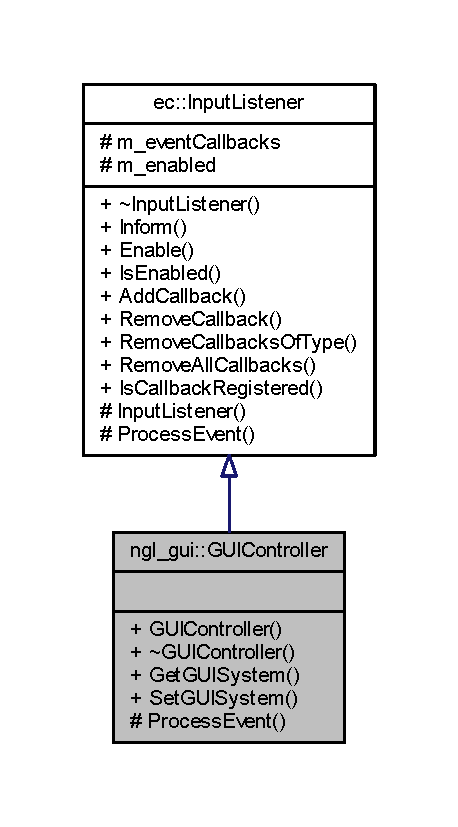
\includegraphics[width=220pt]{classngl__gui_1_1_g_u_i_controller__inherit__graph}
\end{center}
\end{figure}


Collaboration diagram for ngl\+\_\+gui\+:\+:G\+U\+I\+Controller\+:
\nopagebreak
\begin{figure}[H]
\begin{center}
\leavevmode
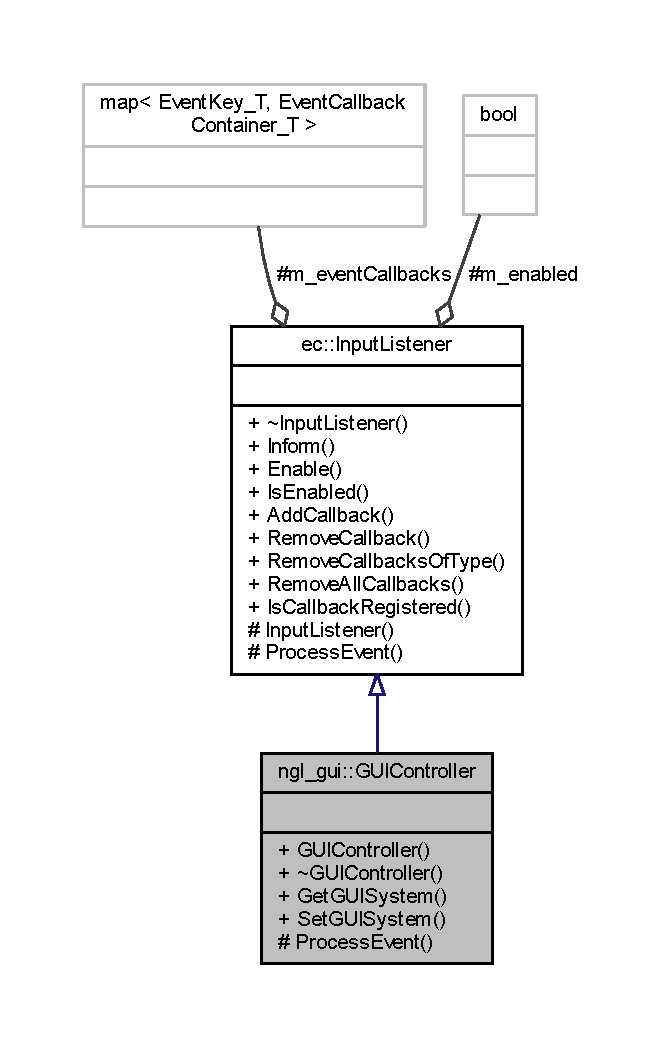
\includegraphics[width=318pt]{classngl__gui_1_1_g_u_i_controller__coll__graph}
\end{center}
\end{figure}
\subsection*{Public Member Functions}
\begin{DoxyCompactItemize}
\item 
\mbox{\hyperlink{classngl__gui_1_1_g_u_i_controller_ac6fe96782bdf72d10859c0a68caf411c}{G\+U\+I\+Controller}} ()
\item 
\mbox{\hyperlink{classngl__gui_1_1_g_u_i_controller_a729c3ba7e7932d954db59172f435e745}{$\sim$\+G\+U\+I\+Controller}} ()
\item 
\mbox{\hyperlink{classngl__gui_1_1_g_u_i_system}{G\+U\+I\+System}} $\ast$ \mbox{\hyperlink{classngl__gui_1_1_g_u_i_controller_a99ed84b859cb86d7d57f1904003a0e16}{Get\+G\+U\+I\+System}} ()
\item 
void \mbox{\hyperlink{classngl__gui_1_1_g_u_i_controller_a5ec3f78019d228572f5797521d5d0507}{Set\+G\+U\+I\+System}} (\mbox{\hyperlink{classngl__gui_1_1_g_u_i_system}{G\+U\+I\+System}} $\ast$gui\+System)
\end{DoxyCompactItemize}
\subsection*{Protected Member Functions}
\begin{DoxyCompactItemize}
\item 
virtual void \mbox{\hyperlink{classngl__gui_1_1_g_u_i_controller_aa0f7e017d386e1e2f02359916be51137}{Process\+Event}} (const \mbox{\hyperlink{structec_1_1_input_event}{ec\+::\+Input\+Event}} \&event) override
\end{DoxyCompactItemize}
\subsection*{Additional Inherited Members}


\subsection{Constructor \& Destructor Documentation}
\mbox{\Hypertarget{classngl__gui_1_1_g_u_i_controller_ac6fe96782bdf72d10859c0a68caf411c}\label{classngl__gui_1_1_g_u_i_controller_ac6fe96782bdf72d10859c0a68caf411c}} 
\index{ngl\+\_\+gui\+::\+G\+U\+I\+Controller@{ngl\+\_\+gui\+::\+G\+U\+I\+Controller}!G\+U\+I\+Controller@{G\+U\+I\+Controller}}
\index{G\+U\+I\+Controller@{G\+U\+I\+Controller}!ngl\+\_\+gui\+::\+G\+U\+I\+Controller@{ngl\+\_\+gui\+::\+G\+U\+I\+Controller}}
\subsubsection{\texorpdfstring{G\+U\+I\+Controller()}{GUIController()}}
{\footnotesize\ttfamily ngl\+\_\+gui\+::\+G\+U\+I\+Controller\+::\+G\+U\+I\+Controller (\begin{DoxyParamCaption}{ }\end{DoxyParamCaption})\hspace{0.3cm}{\ttfamily [explicit]}}

\mbox{\Hypertarget{classngl__gui_1_1_g_u_i_controller_a729c3ba7e7932d954db59172f435e745}\label{classngl__gui_1_1_g_u_i_controller_a729c3ba7e7932d954db59172f435e745}} 
\index{ngl\+\_\+gui\+::\+G\+U\+I\+Controller@{ngl\+\_\+gui\+::\+G\+U\+I\+Controller}!````~G\+U\+I\+Controller@{$\sim$\+G\+U\+I\+Controller}}
\index{````~G\+U\+I\+Controller@{$\sim$\+G\+U\+I\+Controller}!ngl\+\_\+gui\+::\+G\+U\+I\+Controller@{ngl\+\_\+gui\+::\+G\+U\+I\+Controller}}
\subsubsection{\texorpdfstring{$\sim$\+G\+U\+I\+Controller()}{~GUIController()}}
{\footnotesize\ttfamily ngl\+\_\+gui\+::\+G\+U\+I\+Controller\+::$\sim$\+G\+U\+I\+Controller (\begin{DoxyParamCaption}{ }\end{DoxyParamCaption})}



\subsection{Member Function Documentation}
\mbox{\Hypertarget{classngl__gui_1_1_g_u_i_controller_a99ed84b859cb86d7d57f1904003a0e16}\label{classngl__gui_1_1_g_u_i_controller_a99ed84b859cb86d7d57f1904003a0e16}} 
\index{ngl\+\_\+gui\+::\+G\+U\+I\+Controller@{ngl\+\_\+gui\+::\+G\+U\+I\+Controller}!Get\+G\+U\+I\+System@{Get\+G\+U\+I\+System}}
\index{Get\+G\+U\+I\+System@{Get\+G\+U\+I\+System}!ngl\+\_\+gui\+::\+G\+U\+I\+Controller@{ngl\+\_\+gui\+::\+G\+U\+I\+Controller}}
\subsubsection{\texorpdfstring{Get\+G\+U\+I\+System()}{GetGUISystem()}}
{\footnotesize\ttfamily \mbox{\hyperlink{classngl__gui_1_1_g_u_i_system}{ngl\+\_\+gui\+::\+G\+U\+I\+System}} $\ast$ ngl\+\_\+gui\+::\+G\+U\+I\+Controller\+::\+Get\+G\+U\+I\+System (\begin{DoxyParamCaption}{ }\end{DoxyParamCaption})}

\mbox{\Hypertarget{classngl__gui_1_1_g_u_i_controller_aa0f7e017d386e1e2f02359916be51137}\label{classngl__gui_1_1_g_u_i_controller_aa0f7e017d386e1e2f02359916be51137}} 
\index{ngl\+\_\+gui\+::\+G\+U\+I\+Controller@{ngl\+\_\+gui\+::\+G\+U\+I\+Controller}!Process\+Event@{Process\+Event}}
\index{Process\+Event@{Process\+Event}!ngl\+\_\+gui\+::\+G\+U\+I\+Controller@{ngl\+\_\+gui\+::\+G\+U\+I\+Controller}}
\subsubsection{\texorpdfstring{Process\+Event()}{ProcessEvent()}}
{\footnotesize\ttfamily void ngl\+\_\+gui\+::\+G\+U\+I\+Controller\+::\+Process\+Event (\begin{DoxyParamCaption}\item[{const \mbox{\hyperlink{structec_1_1_input_event}{ec\+::\+Input\+Event}} \&}]{event }\end{DoxyParamCaption})\hspace{0.3cm}{\ttfamily [override]}, {\ttfamily [protected]}, {\ttfamily [virtual]}}



Reimplemented from \mbox{\hyperlink{classec_1_1_input_listener_a25ef07efb72ac5c880cbca876ddfe66a}{ec\+::\+Input\+Listener}}.

\mbox{\Hypertarget{classngl__gui_1_1_g_u_i_controller_a5ec3f78019d228572f5797521d5d0507}\label{classngl__gui_1_1_g_u_i_controller_a5ec3f78019d228572f5797521d5d0507}} 
\index{ngl\+\_\+gui\+::\+G\+U\+I\+Controller@{ngl\+\_\+gui\+::\+G\+U\+I\+Controller}!Set\+G\+U\+I\+System@{Set\+G\+U\+I\+System}}
\index{Set\+G\+U\+I\+System@{Set\+G\+U\+I\+System}!ngl\+\_\+gui\+::\+G\+U\+I\+Controller@{ngl\+\_\+gui\+::\+G\+U\+I\+Controller}}
\subsubsection{\texorpdfstring{Set\+G\+U\+I\+System()}{SetGUISystem()}}
{\footnotesize\ttfamily void ngl\+\_\+gui\+::\+G\+U\+I\+Controller\+::\+Set\+G\+U\+I\+System (\begin{DoxyParamCaption}\item[{\mbox{\hyperlink{classngl__gui_1_1_g_u_i_system}{G\+U\+I\+System}} $\ast$}]{gui\+System }\end{DoxyParamCaption})}



The documentation for this class was generated from the following files\+:\begin{DoxyCompactItemize}
\item 
D\+:/\+Library/\+Documents/\+Job/\+Forschungsmaster/\+Projekte/\+Eye\+Candy3\+D/\+Eye\+Candy3\+D/include/\+E\+C3\+D/\+G\+U\+I/\mbox{\hyperlink{_g_u_i_controller_8h}{G\+U\+I\+Controller.\+h}}\item 
D\+:/\+Library/\+Documents/\+Job/\+Forschungsmaster/\+Projekte/\+Eye\+Candy3\+D/\+Eye\+Candy3\+D/src/\+G\+U\+I/\mbox{\hyperlink{_g_u_i_controller_8cpp}{G\+U\+I\+Controller.\+cpp}}\end{DoxyCompactItemize}

\hypertarget{classngl__gui_1_1_g_u_i_model_view_controller}{}\section{ngl\+\_\+gui\+:\+:G\+U\+I\+Model\+View\+Controller Class Reference}
\label{classngl__gui_1_1_g_u_i_model_view_controller}\index{ngl\+\_\+gui\+::\+G\+U\+I\+Model\+View\+Controller@{ngl\+\_\+gui\+::\+G\+U\+I\+Model\+View\+Controller}}


{\ttfamily \#include $<$G\+U\+I\+Model\+View\+Controller.\+h$>$}



Collaboration diagram for ngl\+\_\+gui\+:\+:G\+U\+I\+Model\+View\+Controller\+:\nopagebreak
\begin{figure}[H]
\begin{center}
\leavevmode
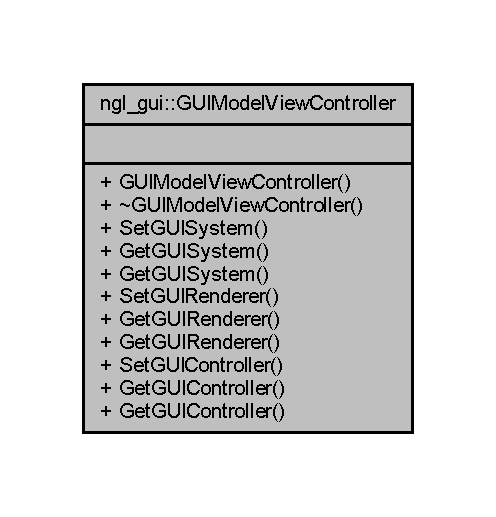
\includegraphics[width=238pt]{classngl__gui_1_1_g_u_i_model_view_controller__coll__graph}
\end{center}
\end{figure}
\subsection*{Public Member Functions}
\begin{DoxyCompactItemize}
\item 
\mbox{\hyperlink{classngl__gui_1_1_g_u_i_model_view_controller_abbe9852d1cc52529dfbdd175c1e27ec1}{G\+U\+I\+Model\+View\+Controller}} ()
\item 
\mbox{\hyperlink{classngl__gui_1_1_g_u_i_model_view_controller_af42d72e9d439309d861161b0a914b88a}{$\sim$\+G\+U\+I\+Model\+View\+Controller}} ()
\item 
void \mbox{\hyperlink{classngl__gui_1_1_g_u_i_model_view_controller_a8f04428e9810125b0fbf14a38a47910d}{Set\+G\+U\+I\+System}} (\mbox{\hyperlink{classngl__gui_1_1_g_u_i_system}{G\+U\+I\+System}} gui\+System)
\item 
const \mbox{\hyperlink{classngl__gui_1_1_g_u_i_system}{G\+U\+I\+System}} \& \mbox{\hyperlink{classngl__gui_1_1_g_u_i_model_view_controller_a3f3dd0ed59d10a38dafd5e7847a8af60}{Get\+G\+U\+I\+System}} () const
\item 
\mbox{\hyperlink{classngl__gui_1_1_g_u_i_system}{G\+U\+I\+System}} \& \mbox{\hyperlink{classngl__gui_1_1_g_u_i_model_view_controller_ad0c0f5afb8f2428a75414ed0d1e5f62d}{Get\+G\+U\+I\+System}} ()
\item 
void \mbox{\hyperlink{classngl__gui_1_1_g_u_i_model_view_controller_a677c75f653cb8334675bf16e65d94294}{Set\+G\+U\+I\+Renderer}} (const \mbox{\hyperlink{classngl__gui_1_1_g_u_i_renderer}{G\+U\+I\+Renderer}} \&gui\+Renderer)
\item 
const \mbox{\hyperlink{classngl__gui_1_1_g_u_i_renderer}{G\+U\+I\+Renderer}} \& \mbox{\hyperlink{classngl__gui_1_1_g_u_i_model_view_controller_a7e0129a2e7d06eb383af11fdfc47baa4}{Get\+G\+U\+I\+Renderer}} () const
\item 
\mbox{\hyperlink{classngl__gui_1_1_g_u_i_renderer}{G\+U\+I\+Renderer}} \& \mbox{\hyperlink{classngl__gui_1_1_g_u_i_model_view_controller_ae8be8d04f4d9f11ed7c2ae0b39091229}{Get\+G\+U\+I\+Renderer}} ()
\item 
void \mbox{\hyperlink{classngl__gui_1_1_g_u_i_model_view_controller_a079bb3f06c3190300ce3dd531c6cb58c}{Set\+G\+U\+I\+Controller}} (std\+::unique\+\_\+ptr$<$ \mbox{\hyperlink{classngl__gui_1_1_g_u_i_controller}{G\+U\+I\+Controller}} $>$ gui\+Controller)
\item 
const \mbox{\hyperlink{classngl__gui_1_1_g_u_i_controller}{G\+U\+I\+Controller}} $\ast$ \mbox{\hyperlink{classngl__gui_1_1_g_u_i_model_view_controller_a3b2bde8db092191a85eb214a11bd3258}{Get\+G\+U\+I\+Controller}} () const
\item 
\mbox{\hyperlink{classngl__gui_1_1_g_u_i_controller}{G\+U\+I\+Controller}} $\ast$ \mbox{\hyperlink{classngl__gui_1_1_g_u_i_model_view_controller_a282cc437e889c538097a4d13c997aa48}{Get\+G\+U\+I\+Controller}} ()
\end{DoxyCompactItemize}


\subsection{Constructor \& Destructor Documentation}
\mbox{\Hypertarget{classngl__gui_1_1_g_u_i_model_view_controller_abbe9852d1cc52529dfbdd175c1e27ec1}\label{classngl__gui_1_1_g_u_i_model_view_controller_abbe9852d1cc52529dfbdd175c1e27ec1}} 
\index{ngl\+\_\+gui\+::\+G\+U\+I\+Model\+View\+Controller@{ngl\+\_\+gui\+::\+G\+U\+I\+Model\+View\+Controller}!G\+U\+I\+Model\+View\+Controller@{G\+U\+I\+Model\+View\+Controller}}
\index{G\+U\+I\+Model\+View\+Controller@{G\+U\+I\+Model\+View\+Controller}!ngl\+\_\+gui\+::\+G\+U\+I\+Model\+View\+Controller@{ngl\+\_\+gui\+::\+G\+U\+I\+Model\+View\+Controller}}
\subsubsection{\texorpdfstring{G\+U\+I\+Model\+View\+Controller()}{GUIModelViewController()}}
{\footnotesize\ttfamily ngl\+\_\+gui\+::\+G\+U\+I\+Model\+View\+Controller\+::\+G\+U\+I\+Model\+View\+Controller (\begin{DoxyParamCaption}{ }\end{DoxyParamCaption})\hspace{0.3cm}{\ttfamily [explicit]}}

\mbox{\Hypertarget{classngl__gui_1_1_g_u_i_model_view_controller_af42d72e9d439309d861161b0a914b88a}\label{classngl__gui_1_1_g_u_i_model_view_controller_af42d72e9d439309d861161b0a914b88a}} 
\index{ngl\+\_\+gui\+::\+G\+U\+I\+Model\+View\+Controller@{ngl\+\_\+gui\+::\+G\+U\+I\+Model\+View\+Controller}!````~G\+U\+I\+Model\+View\+Controller@{$\sim$\+G\+U\+I\+Model\+View\+Controller}}
\index{````~G\+U\+I\+Model\+View\+Controller@{$\sim$\+G\+U\+I\+Model\+View\+Controller}!ngl\+\_\+gui\+::\+G\+U\+I\+Model\+View\+Controller@{ngl\+\_\+gui\+::\+G\+U\+I\+Model\+View\+Controller}}
\subsubsection{\texorpdfstring{$\sim$\+G\+U\+I\+Model\+View\+Controller()}{~GUIModelViewController()}}
{\footnotesize\ttfamily ngl\+\_\+gui\+::\+G\+U\+I\+Model\+View\+Controller\+::$\sim$\+G\+U\+I\+Model\+View\+Controller (\begin{DoxyParamCaption}{ }\end{DoxyParamCaption})}



\subsection{Member Function Documentation}
\mbox{\Hypertarget{classngl__gui_1_1_g_u_i_model_view_controller_a3b2bde8db092191a85eb214a11bd3258}\label{classngl__gui_1_1_g_u_i_model_view_controller_a3b2bde8db092191a85eb214a11bd3258}} 
\index{ngl\+\_\+gui\+::\+G\+U\+I\+Model\+View\+Controller@{ngl\+\_\+gui\+::\+G\+U\+I\+Model\+View\+Controller}!Get\+G\+U\+I\+Controller@{Get\+G\+U\+I\+Controller}}
\index{Get\+G\+U\+I\+Controller@{Get\+G\+U\+I\+Controller}!ngl\+\_\+gui\+::\+G\+U\+I\+Model\+View\+Controller@{ngl\+\_\+gui\+::\+G\+U\+I\+Model\+View\+Controller}}
\subsubsection{\texorpdfstring{Get\+G\+U\+I\+Controller()}{GetGUIController()}\hspace{0.1cm}{\footnotesize\ttfamily [1/2]}}
{\footnotesize\ttfamily const \mbox{\hyperlink{classngl__gui_1_1_g_u_i_controller}{ngl\+\_\+gui\+::\+G\+U\+I\+Controller}} $\ast$ ngl\+\_\+gui\+::\+G\+U\+I\+Model\+View\+Controller\+::\+Get\+G\+U\+I\+Controller (\begin{DoxyParamCaption}{ }\end{DoxyParamCaption}) const}

\mbox{\Hypertarget{classngl__gui_1_1_g_u_i_model_view_controller_a282cc437e889c538097a4d13c997aa48}\label{classngl__gui_1_1_g_u_i_model_view_controller_a282cc437e889c538097a4d13c997aa48}} 
\index{ngl\+\_\+gui\+::\+G\+U\+I\+Model\+View\+Controller@{ngl\+\_\+gui\+::\+G\+U\+I\+Model\+View\+Controller}!Get\+G\+U\+I\+Controller@{Get\+G\+U\+I\+Controller}}
\index{Get\+G\+U\+I\+Controller@{Get\+G\+U\+I\+Controller}!ngl\+\_\+gui\+::\+G\+U\+I\+Model\+View\+Controller@{ngl\+\_\+gui\+::\+G\+U\+I\+Model\+View\+Controller}}
\subsubsection{\texorpdfstring{Get\+G\+U\+I\+Controller()}{GetGUIController()}\hspace{0.1cm}{\footnotesize\ttfamily [2/2]}}
{\footnotesize\ttfamily \mbox{\hyperlink{classngl__gui_1_1_g_u_i_controller}{ngl\+\_\+gui\+::\+G\+U\+I\+Controller}} $\ast$ ngl\+\_\+gui\+::\+G\+U\+I\+Model\+View\+Controller\+::\+Get\+G\+U\+I\+Controller (\begin{DoxyParamCaption}{ }\end{DoxyParamCaption})}

\mbox{\Hypertarget{classngl__gui_1_1_g_u_i_model_view_controller_a7e0129a2e7d06eb383af11fdfc47baa4}\label{classngl__gui_1_1_g_u_i_model_view_controller_a7e0129a2e7d06eb383af11fdfc47baa4}} 
\index{ngl\+\_\+gui\+::\+G\+U\+I\+Model\+View\+Controller@{ngl\+\_\+gui\+::\+G\+U\+I\+Model\+View\+Controller}!Get\+G\+U\+I\+Renderer@{Get\+G\+U\+I\+Renderer}}
\index{Get\+G\+U\+I\+Renderer@{Get\+G\+U\+I\+Renderer}!ngl\+\_\+gui\+::\+G\+U\+I\+Model\+View\+Controller@{ngl\+\_\+gui\+::\+G\+U\+I\+Model\+View\+Controller}}
\subsubsection{\texorpdfstring{Get\+G\+U\+I\+Renderer()}{GetGUIRenderer()}\hspace{0.1cm}{\footnotesize\ttfamily [1/2]}}
{\footnotesize\ttfamily const \mbox{\hyperlink{classngl__gui_1_1_g_u_i_renderer}{ngl\+\_\+gui\+::\+G\+U\+I\+Renderer}} \& ngl\+\_\+gui\+::\+G\+U\+I\+Model\+View\+Controller\+::\+Get\+G\+U\+I\+Renderer (\begin{DoxyParamCaption}{ }\end{DoxyParamCaption}) const}

\mbox{\Hypertarget{classngl__gui_1_1_g_u_i_model_view_controller_ae8be8d04f4d9f11ed7c2ae0b39091229}\label{classngl__gui_1_1_g_u_i_model_view_controller_ae8be8d04f4d9f11ed7c2ae0b39091229}} 
\index{ngl\+\_\+gui\+::\+G\+U\+I\+Model\+View\+Controller@{ngl\+\_\+gui\+::\+G\+U\+I\+Model\+View\+Controller}!Get\+G\+U\+I\+Renderer@{Get\+G\+U\+I\+Renderer}}
\index{Get\+G\+U\+I\+Renderer@{Get\+G\+U\+I\+Renderer}!ngl\+\_\+gui\+::\+G\+U\+I\+Model\+View\+Controller@{ngl\+\_\+gui\+::\+G\+U\+I\+Model\+View\+Controller}}
\subsubsection{\texorpdfstring{Get\+G\+U\+I\+Renderer()}{GetGUIRenderer()}\hspace{0.1cm}{\footnotesize\ttfamily [2/2]}}
{\footnotesize\ttfamily \mbox{\hyperlink{classngl__gui_1_1_g_u_i_renderer}{ngl\+\_\+gui\+::\+G\+U\+I\+Renderer}} \& ngl\+\_\+gui\+::\+G\+U\+I\+Model\+View\+Controller\+::\+Get\+G\+U\+I\+Renderer (\begin{DoxyParamCaption}{ }\end{DoxyParamCaption})}

\mbox{\Hypertarget{classngl__gui_1_1_g_u_i_model_view_controller_a3f3dd0ed59d10a38dafd5e7847a8af60}\label{classngl__gui_1_1_g_u_i_model_view_controller_a3f3dd0ed59d10a38dafd5e7847a8af60}} 
\index{ngl\+\_\+gui\+::\+G\+U\+I\+Model\+View\+Controller@{ngl\+\_\+gui\+::\+G\+U\+I\+Model\+View\+Controller}!Get\+G\+U\+I\+System@{Get\+G\+U\+I\+System}}
\index{Get\+G\+U\+I\+System@{Get\+G\+U\+I\+System}!ngl\+\_\+gui\+::\+G\+U\+I\+Model\+View\+Controller@{ngl\+\_\+gui\+::\+G\+U\+I\+Model\+View\+Controller}}
\subsubsection{\texorpdfstring{Get\+G\+U\+I\+System()}{GetGUISystem()}\hspace{0.1cm}{\footnotesize\ttfamily [1/2]}}
{\footnotesize\ttfamily const \mbox{\hyperlink{classngl__gui_1_1_g_u_i_system}{ngl\+\_\+gui\+::\+G\+U\+I\+System}} \& ngl\+\_\+gui\+::\+G\+U\+I\+Model\+View\+Controller\+::\+Get\+G\+U\+I\+System (\begin{DoxyParamCaption}{ }\end{DoxyParamCaption}) const}

\mbox{\Hypertarget{classngl__gui_1_1_g_u_i_model_view_controller_ad0c0f5afb8f2428a75414ed0d1e5f62d}\label{classngl__gui_1_1_g_u_i_model_view_controller_ad0c0f5afb8f2428a75414ed0d1e5f62d}} 
\index{ngl\+\_\+gui\+::\+G\+U\+I\+Model\+View\+Controller@{ngl\+\_\+gui\+::\+G\+U\+I\+Model\+View\+Controller}!Get\+G\+U\+I\+System@{Get\+G\+U\+I\+System}}
\index{Get\+G\+U\+I\+System@{Get\+G\+U\+I\+System}!ngl\+\_\+gui\+::\+G\+U\+I\+Model\+View\+Controller@{ngl\+\_\+gui\+::\+G\+U\+I\+Model\+View\+Controller}}
\subsubsection{\texorpdfstring{Get\+G\+U\+I\+System()}{GetGUISystem()}\hspace{0.1cm}{\footnotesize\ttfamily [2/2]}}
{\footnotesize\ttfamily \mbox{\hyperlink{classngl__gui_1_1_g_u_i_system}{ngl\+\_\+gui\+::\+G\+U\+I\+System}} \& ngl\+\_\+gui\+::\+G\+U\+I\+Model\+View\+Controller\+::\+Get\+G\+U\+I\+System (\begin{DoxyParamCaption}{ }\end{DoxyParamCaption})}

\mbox{\Hypertarget{classngl__gui_1_1_g_u_i_model_view_controller_a079bb3f06c3190300ce3dd531c6cb58c}\label{classngl__gui_1_1_g_u_i_model_view_controller_a079bb3f06c3190300ce3dd531c6cb58c}} 
\index{ngl\+\_\+gui\+::\+G\+U\+I\+Model\+View\+Controller@{ngl\+\_\+gui\+::\+G\+U\+I\+Model\+View\+Controller}!Set\+G\+U\+I\+Controller@{Set\+G\+U\+I\+Controller}}
\index{Set\+G\+U\+I\+Controller@{Set\+G\+U\+I\+Controller}!ngl\+\_\+gui\+::\+G\+U\+I\+Model\+View\+Controller@{ngl\+\_\+gui\+::\+G\+U\+I\+Model\+View\+Controller}}
\subsubsection{\texorpdfstring{Set\+G\+U\+I\+Controller()}{SetGUIController()}}
{\footnotesize\ttfamily void ngl\+\_\+gui\+::\+G\+U\+I\+Model\+View\+Controller\+::\+Set\+G\+U\+I\+Controller (\begin{DoxyParamCaption}\item[{std\+::unique\+\_\+ptr$<$ \mbox{\hyperlink{classngl__gui_1_1_g_u_i_controller}{G\+U\+I\+Controller}} $>$}]{gui\+Controller }\end{DoxyParamCaption})}

\mbox{\Hypertarget{classngl__gui_1_1_g_u_i_model_view_controller_a677c75f653cb8334675bf16e65d94294}\label{classngl__gui_1_1_g_u_i_model_view_controller_a677c75f653cb8334675bf16e65d94294}} 
\index{ngl\+\_\+gui\+::\+G\+U\+I\+Model\+View\+Controller@{ngl\+\_\+gui\+::\+G\+U\+I\+Model\+View\+Controller}!Set\+G\+U\+I\+Renderer@{Set\+G\+U\+I\+Renderer}}
\index{Set\+G\+U\+I\+Renderer@{Set\+G\+U\+I\+Renderer}!ngl\+\_\+gui\+::\+G\+U\+I\+Model\+View\+Controller@{ngl\+\_\+gui\+::\+G\+U\+I\+Model\+View\+Controller}}
\subsubsection{\texorpdfstring{Set\+G\+U\+I\+Renderer()}{SetGUIRenderer()}}
{\footnotesize\ttfamily void ngl\+\_\+gui\+::\+G\+U\+I\+Model\+View\+Controller\+::\+Set\+G\+U\+I\+Renderer (\begin{DoxyParamCaption}\item[{const \mbox{\hyperlink{classngl__gui_1_1_g_u_i_renderer}{G\+U\+I\+Renderer}} \&}]{gui\+Renderer }\end{DoxyParamCaption})}

\mbox{\Hypertarget{classngl__gui_1_1_g_u_i_model_view_controller_a8f04428e9810125b0fbf14a38a47910d}\label{classngl__gui_1_1_g_u_i_model_view_controller_a8f04428e9810125b0fbf14a38a47910d}} 
\index{ngl\+\_\+gui\+::\+G\+U\+I\+Model\+View\+Controller@{ngl\+\_\+gui\+::\+G\+U\+I\+Model\+View\+Controller}!Set\+G\+U\+I\+System@{Set\+G\+U\+I\+System}}
\index{Set\+G\+U\+I\+System@{Set\+G\+U\+I\+System}!ngl\+\_\+gui\+::\+G\+U\+I\+Model\+View\+Controller@{ngl\+\_\+gui\+::\+G\+U\+I\+Model\+View\+Controller}}
\subsubsection{\texorpdfstring{Set\+G\+U\+I\+System()}{SetGUISystem()}}
{\footnotesize\ttfamily void ngl\+\_\+gui\+::\+G\+U\+I\+Model\+View\+Controller\+::\+Set\+G\+U\+I\+System (\begin{DoxyParamCaption}\item[{\mbox{\hyperlink{classngl__gui_1_1_g_u_i_system}{G\+U\+I\+System}}}]{gui\+System }\end{DoxyParamCaption})}



The documentation for this class was generated from the following files\+:\begin{DoxyCompactItemize}
\item 
D\+:/\+Library/\+Documents/\+Job/\+Forschungsmaster/\+Projekte/\+Eye\+Candy3\+D/\+Eye\+Candy3\+D/include/\+E\+C3\+D/\+G\+U\+I/\mbox{\hyperlink{_g_u_i_model_view_controller_8h}{G\+U\+I\+Model\+View\+Controller.\+h}}\item 
D\+:/\+Library/\+Documents/\+Job/\+Forschungsmaster/\+Projekte/\+Eye\+Candy3\+D/\+Eye\+Candy3\+D/src/\+G\+U\+I/\mbox{\hyperlink{_g_u_i_model_view_controller_8cpp}{G\+U\+I\+Model\+View\+Controller.\+cpp}}\end{DoxyCompactItemize}

\hypertarget{classngl__gui_1_1_g_u_i_renderer}{}\section{ngl\+\_\+gui\+:\+:G\+U\+I\+Renderer Class Reference}
\label{classngl__gui_1_1_g_u_i_renderer}\index{ngl\+\_\+gui\+::\+G\+U\+I\+Renderer@{ngl\+\_\+gui\+::\+G\+U\+I\+Renderer}}


{\ttfamily \#include $<$G\+U\+I\+Renderer.\+h$>$}



Collaboration diagram for ngl\+\_\+gui\+:\+:G\+U\+I\+Renderer\+:\nopagebreak
\begin{figure}[H]
\begin{center}
\leavevmode
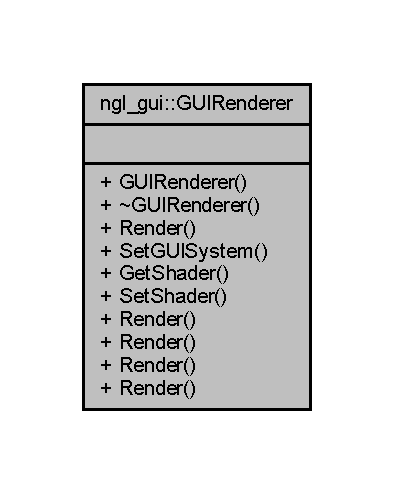
\includegraphics[width=189pt]{classngl__gui_1_1_g_u_i_renderer__coll__graph}
\end{center}
\end{figure}
\subsection*{Public Member Functions}
\begin{DoxyCompactItemize}
\item 
\mbox{\hyperlink{classngl__gui_1_1_g_u_i_renderer_ad3a022f8ea3ad488692223baf808d103}{G\+U\+I\+Renderer}} ()
\item 
\mbox{\hyperlink{classngl__gui_1_1_g_u_i_renderer_a73dd3d294eb6e79e3b874942d4a95b5a}{$\sim$\+G\+U\+I\+Renderer}} ()
\item 
void \mbox{\hyperlink{classngl__gui_1_1_g_u_i_renderer_a616aa4e5bc587896848b2523686824a7}{Render}} (\mbox{\hyperlink{structngl__gui_1_1_g_u_i_rendering_parameter_list}{G\+U\+I\+Rendering\+Parameter\+List}} params)
\item 
void \mbox{\hyperlink{classngl__gui_1_1_g_u_i_renderer_a80a4dfa6dbf0df163b24687aa1eea9f1}{Set\+G\+U\+I\+System}} (\mbox{\hyperlink{classngl__gui_1_1_g_u_i_system}{G\+U\+I\+System}} $\ast$gui\+System)
\item 
\mbox{\hyperlink{classec_1_1_shader}{ec\+::\+Shader}} $\ast$ \mbox{\hyperlink{classngl__gui_1_1_g_u_i_renderer_a7c835ff437f3781674a676aaea4546d6}{Get\+Shader}} ()
\item 
void \mbox{\hyperlink{classngl__gui_1_1_g_u_i_renderer_aa1744c6a938e609a87d55a8efece3993}{Set\+Shader}} (\mbox{\hyperlink{classec_1_1_shader}{ec\+::\+Shader}} $\ast$shader)
\item 
void \mbox{\hyperlink{classngl__gui_1_1_g_u_i_renderer_af149928da5c1cb43fb491823a1b264b8}{Render}} (\mbox{\hyperlink{classngl__gui_1_1_widget}{Widget}} $\ast$widget, \mbox{\hyperlink{classngl__gui_1_1_g_u_i_rendering_context}{G\+U\+I\+Rendering\+Context}} \&context)
\item 
void \mbox{\hyperlink{classngl__gui_1_1_g_u_i_renderer_a4c786cb952ffa1b60e47e67ace0c27db}{Render}} (\mbox{\hyperlink{classngl__gui_1_1_text}{Text}} $\ast$text, \mbox{\hyperlink{classngl__gui_1_1_g_u_i_rendering_context}{G\+U\+I\+Rendering\+Context}} \&context)
\item 
void \mbox{\hyperlink{classngl__gui_1_1_g_u_i_renderer_ae4152d9b062f2bc5910645469b265347}{Render}} (\mbox{\hyperlink{classngl__gui_1_1_screen}{Screen}} $\ast$screen, \mbox{\hyperlink{classngl__gui_1_1_g_u_i_rendering_context}{G\+U\+I\+Rendering\+Context}} \&context)
\item 
void \mbox{\hyperlink{classngl__gui_1_1_g_u_i_renderer_a1bd189925c3324cef53d59168aa75d43}{Render}} (\mbox{\hyperlink{classngl__gui_1_1_window}{Window}} $\ast$window, \mbox{\hyperlink{classngl__gui_1_1_g_u_i_rendering_context}{G\+U\+I\+Rendering\+Context}} \&context)
\end{DoxyCompactItemize}


\subsection{Constructor \& Destructor Documentation}
\mbox{\Hypertarget{classngl__gui_1_1_g_u_i_renderer_ad3a022f8ea3ad488692223baf808d103}\label{classngl__gui_1_1_g_u_i_renderer_ad3a022f8ea3ad488692223baf808d103}} 
\index{ngl\+\_\+gui\+::\+G\+U\+I\+Renderer@{ngl\+\_\+gui\+::\+G\+U\+I\+Renderer}!G\+U\+I\+Renderer@{G\+U\+I\+Renderer}}
\index{G\+U\+I\+Renderer@{G\+U\+I\+Renderer}!ngl\+\_\+gui\+::\+G\+U\+I\+Renderer@{ngl\+\_\+gui\+::\+G\+U\+I\+Renderer}}
\subsubsection{\texorpdfstring{G\+U\+I\+Renderer()}{GUIRenderer()}}
{\footnotesize\ttfamily ngl\+\_\+gui\+::\+G\+U\+I\+Renderer\+::\+G\+U\+I\+Renderer (\begin{DoxyParamCaption}{ }\end{DoxyParamCaption})\hspace{0.3cm}{\ttfamily [explicit]}}

\mbox{\Hypertarget{classngl__gui_1_1_g_u_i_renderer_a73dd3d294eb6e79e3b874942d4a95b5a}\label{classngl__gui_1_1_g_u_i_renderer_a73dd3d294eb6e79e3b874942d4a95b5a}} 
\index{ngl\+\_\+gui\+::\+G\+U\+I\+Renderer@{ngl\+\_\+gui\+::\+G\+U\+I\+Renderer}!````~G\+U\+I\+Renderer@{$\sim$\+G\+U\+I\+Renderer}}
\index{````~G\+U\+I\+Renderer@{$\sim$\+G\+U\+I\+Renderer}!ngl\+\_\+gui\+::\+G\+U\+I\+Renderer@{ngl\+\_\+gui\+::\+G\+U\+I\+Renderer}}
\subsubsection{\texorpdfstring{$\sim$\+G\+U\+I\+Renderer()}{~GUIRenderer()}}
{\footnotesize\ttfamily ngl\+\_\+gui\+::\+G\+U\+I\+Renderer\+::$\sim$\+G\+U\+I\+Renderer (\begin{DoxyParamCaption}{ }\end{DoxyParamCaption})}



\subsection{Member Function Documentation}
\mbox{\Hypertarget{classngl__gui_1_1_g_u_i_renderer_a7c835ff437f3781674a676aaea4546d6}\label{classngl__gui_1_1_g_u_i_renderer_a7c835ff437f3781674a676aaea4546d6}} 
\index{ngl\+\_\+gui\+::\+G\+U\+I\+Renderer@{ngl\+\_\+gui\+::\+G\+U\+I\+Renderer}!Get\+Shader@{Get\+Shader}}
\index{Get\+Shader@{Get\+Shader}!ngl\+\_\+gui\+::\+G\+U\+I\+Renderer@{ngl\+\_\+gui\+::\+G\+U\+I\+Renderer}}
\subsubsection{\texorpdfstring{Get\+Shader()}{GetShader()}}
{\footnotesize\ttfamily \mbox{\hyperlink{classec_1_1_shader}{ec\+::\+Shader}} $\ast$ ngl\+\_\+gui\+::\+G\+U\+I\+Renderer\+::\+Get\+Shader (\begin{DoxyParamCaption}{ }\end{DoxyParamCaption})}

\mbox{\Hypertarget{classngl__gui_1_1_g_u_i_renderer_a616aa4e5bc587896848b2523686824a7}\label{classngl__gui_1_1_g_u_i_renderer_a616aa4e5bc587896848b2523686824a7}} 
\index{ngl\+\_\+gui\+::\+G\+U\+I\+Renderer@{ngl\+\_\+gui\+::\+G\+U\+I\+Renderer}!Render@{Render}}
\index{Render@{Render}!ngl\+\_\+gui\+::\+G\+U\+I\+Renderer@{ngl\+\_\+gui\+::\+G\+U\+I\+Renderer}}
\subsubsection{\texorpdfstring{Render()}{Render()}\hspace{0.1cm}{\footnotesize\ttfamily [1/5]}}
{\footnotesize\ttfamily void ngl\+\_\+gui\+::\+G\+U\+I\+Renderer\+::\+Render (\begin{DoxyParamCaption}\item[{\mbox{\hyperlink{structngl__gui_1_1_g_u_i_rendering_parameter_list}{G\+U\+I\+Rendering\+Parameter\+List}}}]{params }\end{DoxyParamCaption})}

\mbox{\Hypertarget{classngl__gui_1_1_g_u_i_renderer_af149928da5c1cb43fb491823a1b264b8}\label{classngl__gui_1_1_g_u_i_renderer_af149928da5c1cb43fb491823a1b264b8}} 
\index{ngl\+\_\+gui\+::\+G\+U\+I\+Renderer@{ngl\+\_\+gui\+::\+G\+U\+I\+Renderer}!Render@{Render}}
\index{Render@{Render}!ngl\+\_\+gui\+::\+G\+U\+I\+Renderer@{ngl\+\_\+gui\+::\+G\+U\+I\+Renderer}}
\subsubsection{\texorpdfstring{Render()}{Render()}\hspace{0.1cm}{\footnotesize\ttfamily [2/5]}}
{\footnotesize\ttfamily void ngl\+\_\+gui\+::\+G\+U\+I\+Renderer\+::\+Render (\begin{DoxyParamCaption}\item[{\mbox{\hyperlink{classngl__gui_1_1_widget}{Widget}} $\ast$}]{widget,  }\item[{\mbox{\hyperlink{classngl__gui_1_1_g_u_i_rendering_context}{G\+U\+I\+Rendering\+Context}} \&}]{context }\end{DoxyParamCaption})}

\mbox{\Hypertarget{classngl__gui_1_1_g_u_i_renderer_a4c786cb952ffa1b60e47e67ace0c27db}\label{classngl__gui_1_1_g_u_i_renderer_a4c786cb952ffa1b60e47e67ace0c27db}} 
\index{ngl\+\_\+gui\+::\+G\+U\+I\+Renderer@{ngl\+\_\+gui\+::\+G\+U\+I\+Renderer}!Render@{Render}}
\index{Render@{Render}!ngl\+\_\+gui\+::\+G\+U\+I\+Renderer@{ngl\+\_\+gui\+::\+G\+U\+I\+Renderer}}
\subsubsection{\texorpdfstring{Render()}{Render()}\hspace{0.1cm}{\footnotesize\ttfamily [3/5]}}
{\footnotesize\ttfamily void ngl\+\_\+gui\+::\+G\+U\+I\+Renderer\+::\+Render (\begin{DoxyParamCaption}\item[{\mbox{\hyperlink{classngl__gui_1_1_text}{Text}} $\ast$}]{text,  }\item[{\mbox{\hyperlink{classngl__gui_1_1_g_u_i_rendering_context}{G\+U\+I\+Rendering\+Context}} \&}]{context }\end{DoxyParamCaption})}

\mbox{\Hypertarget{classngl__gui_1_1_g_u_i_renderer_ae4152d9b062f2bc5910645469b265347}\label{classngl__gui_1_1_g_u_i_renderer_ae4152d9b062f2bc5910645469b265347}} 
\index{ngl\+\_\+gui\+::\+G\+U\+I\+Renderer@{ngl\+\_\+gui\+::\+G\+U\+I\+Renderer}!Render@{Render}}
\index{Render@{Render}!ngl\+\_\+gui\+::\+G\+U\+I\+Renderer@{ngl\+\_\+gui\+::\+G\+U\+I\+Renderer}}
\subsubsection{\texorpdfstring{Render()}{Render()}\hspace{0.1cm}{\footnotesize\ttfamily [4/5]}}
{\footnotesize\ttfamily void ngl\+\_\+gui\+::\+G\+U\+I\+Renderer\+::\+Render (\begin{DoxyParamCaption}\item[{\mbox{\hyperlink{classngl__gui_1_1_screen}{Screen}} $\ast$}]{screen,  }\item[{\mbox{\hyperlink{classngl__gui_1_1_g_u_i_rendering_context}{G\+U\+I\+Rendering\+Context}} \&}]{context }\end{DoxyParamCaption})}

\mbox{\Hypertarget{classngl__gui_1_1_g_u_i_renderer_a1bd189925c3324cef53d59168aa75d43}\label{classngl__gui_1_1_g_u_i_renderer_a1bd189925c3324cef53d59168aa75d43}} 
\index{ngl\+\_\+gui\+::\+G\+U\+I\+Renderer@{ngl\+\_\+gui\+::\+G\+U\+I\+Renderer}!Render@{Render}}
\index{Render@{Render}!ngl\+\_\+gui\+::\+G\+U\+I\+Renderer@{ngl\+\_\+gui\+::\+G\+U\+I\+Renderer}}
\subsubsection{\texorpdfstring{Render()}{Render()}\hspace{0.1cm}{\footnotesize\ttfamily [5/5]}}
{\footnotesize\ttfamily void ngl\+\_\+gui\+::\+G\+U\+I\+Renderer\+::\+Render (\begin{DoxyParamCaption}\item[{\mbox{\hyperlink{classngl__gui_1_1_window}{Window}} $\ast$}]{window,  }\item[{\mbox{\hyperlink{classngl__gui_1_1_g_u_i_rendering_context}{G\+U\+I\+Rendering\+Context}} \&}]{context }\end{DoxyParamCaption})}

\mbox{\Hypertarget{classngl__gui_1_1_g_u_i_renderer_a80a4dfa6dbf0df163b24687aa1eea9f1}\label{classngl__gui_1_1_g_u_i_renderer_a80a4dfa6dbf0df163b24687aa1eea9f1}} 
\index{ngl\+\_\+gui\+::\+G\+U\+I\+Renderer@{ngl\+\_\+gui\+::\+G\+U\+I\+Renderer}!Set\+G\+U\+I\+System@{Set\+G\+U\+I\+System}}
\index{Set\+G\+U\+I\+System@{Set\+G\+U\+I\+System}!ngl\+\_\+gui\+::\+G\+U\+I\+Renderer@{ngl\+\_\+gui\+::\+G\+U\+I\+Renderer}}
\subsubsection{\texorpdfstring{Set\+G\+U\+I\+System()}{SetGUISystem()}}
{\footnotesize\ttfamily void ngl\+\_\+gui\+::\+G\+U\+I\+Renderer\+::\+Set\+G\+U\+I\+System (\begin{DoxyParamCaption}\item[{\mbox{\hyperlink{classngl__gui_1_1_g_u_i_system}{G\+U\+I\+System}} $\ast$}]{gui\+System }\end{DoxyParamCaption})}

\mbox{\Hypertarget{classngl__gui_1_1_g_u_i_renderer_aa1744c6a938e609a87d55a8efece3993}\label{classngl__gui_1_1_g_u_i_renderer_aa1744c6a938e609a87d55a8efece3993}} 
\index{ngl\+\_\+gui\+::\+G\+U\+I\+Renderer@{ngl\+\_\+gui\+::\+G\+U\+I\+Renderer}!Set\+Shader@{Set\+Shader}}
\index{Set\+Shader@{Set\+Shader}!ngl\+\_\+gui\+::\+G\+U\+I\+Renderer@{ngl\+\_\+gui\+::\+G\+U\+I\+Renderer}}
\subsubsection{\texorpdfstring{Set\+Shader()}{SetShader()}}
{\footnotesize\ttfamily void ngl\+\_\+gui\+::\+G\+U\+I\+Renderer\+::\+Set\+Shader (\begin{DoxyParamCaption}\item[{\mbox{\hyperlink{classec_1_1_shader}{ec\+::\+Shader}} $\ast$}]{shader }\end{DoxyParamCaption})}



The documentation for this class was generated from the following files\+:\begin{DoxyCompactItemize}
\item 
D\+:/\+Library/\+Documents/\+Job/\+Forschungsmaster/\+Projekte/\+Eye\+Candy3\+D/\+Eye\+Candy3\+D/include/\+E\+C3\+D/\+G\+U\+I/\mbox{\hyperlink{_g_u_i_renderer_8h}{G\+U\+I\+Renderer.\+h}}\item 
D\+:/\+Library/\+Documents/\+Job/\+Forschungsmaster/\+Projekte/\+Eye\+Candy3\+D/\+Eye\+Candy3\+D/src/\+G\+U\+I/\mbox{\hyperlink{_g_u_i_renderer_8cpp}{G\+U\+I\+Renderer.\+cpp}}\end{DoxyCompactItemize}

\hypertarget{classngl__gui_1_1_g_u_i_rendering_context}{}\section{ngl\+\_\+gui\+:\+:G\+U\+I\+Rendering\+Context Class Reference}
\label{classngl__gui_1_1_g_u_i_rendering_context}\index{ngl\+\_\+gui\+::\+G\+U\+I\+Rendering\+Context@{ngl\+\_\+gui\+::\+G\+U\+I\+Rendering\+Context}}


{\ttfamily \#include $<$G\+U\+I\+Renderer.\+h$>$}



Collaboration diagram for ngl\+\_\+gui\+:\+:G\+U\+I\+Rendering\+Context\+:\nopagebreak
\begin{figure}[H]
\begin{center}
\leavevmode
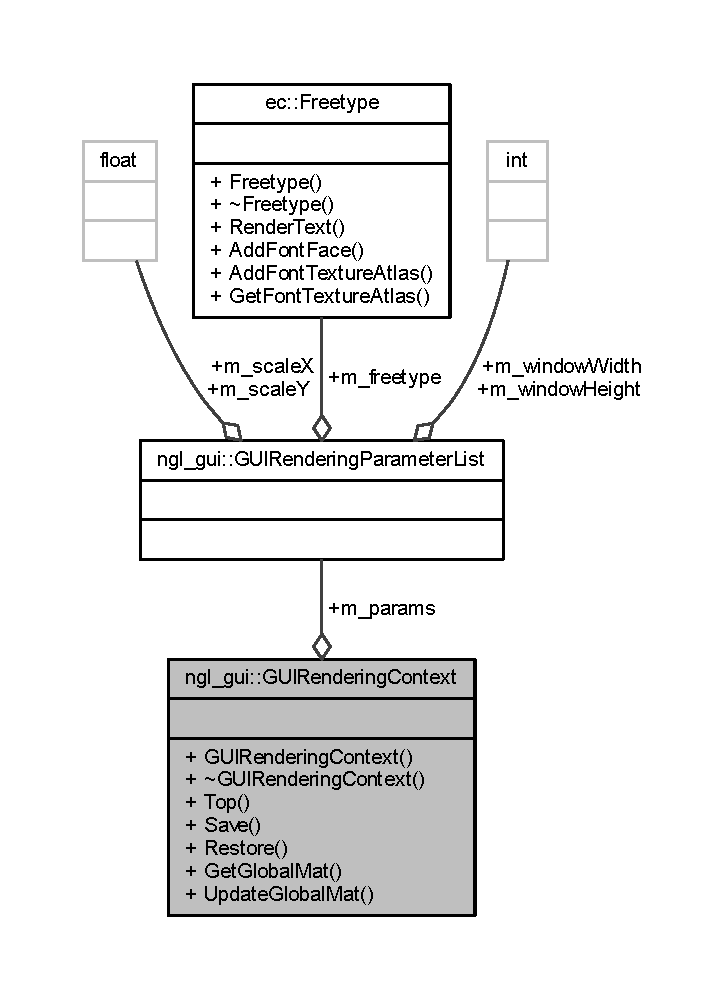
\includegraphics[width=349pt]{classngl__gui_1_1_g_u_i_rendering_context__coll__graph}
\end{center}
\end{figure}
\subsection*{Public Member Functions}
\begin{DoxyCompactItemize}
\item 
\mbox{\hyperlink{classngl__gui_1_1_g_u_i_rendering_context_ae9f289fcceb629044ac36ca31f539ef5}{G\+U\+I\+Rendering\+Context}} ()
\item 
\mbox{\hyperlink{classngl__gui_1_1_g_u_i_rendering_context_a5d94526a789e2d51f7d0007a7052ff71}{$\sim$\+G\+U\+I\+Rendering\+Context}} ()
\item 
const glm\+::mat4 \& \mbox{\hyperlink{classngl__gui_1_1_g_u_i_rendering_context_a3c8be8d1ee58468ebf2da08d55aeb340}{Top}} () const
\item 
void \mbox{\hyperlink{classngl__gui_1_1_g_u_i_rendering_context_a675df7cfcf7e47ebd1a855925c5e870e}{Save}} (const glm\+::mat4 \&mat)
\item 
void \mbox{\hyperlink{classngl__gui_1_1_g_u_i_rendering_context_aca19dc6c7b09be476dc7eac1c5d59798}{Restore}} ()
\item 
const glm\+::mat4 \& \mbox{\hyperlink{classngl__gui_1_1_g_u_i_rendering_context_a726b794550ac8969c6e2d160feadda63}{Get\+Global\+Mat}} ()
\item 
void \mbox{\hyperlink{classngl__gui_1_1_g_u_i_rendering_context_a97eb947aabbb15f4a816f0273bb8afd8}{Update\+Global\+Mat}} (\mbox{\hyperlink{classngl__gui_1_1_widget}{Widget}} $\ast$widget)
\end{DoxyCompactItemize}
\subsection*{Public Attributes}
\begin{DoxyCompactItemize}
\item 
\mbox{\hyperlink{structngl__gui_1_1_g_u_i_rendering_parameter_list}{G\+U\+I\+Rendering\+Parameter\+List}} \mbox{\hyperlink{classngl__gui_1_1_g_u_i_rendering_context_a6eec556788614881c0d087fd52e42b43}{m\+\_\+params}}
\end{DoxyCompactItemize}


\subsection{Constructor \& Destructor Documentation}
\mbox{\Hypertarget{classngl__gui_1_1_g_u_i_rendering_context_ae9f289fcceb629044ac36ca31f539ef5}\label{classngl__gui_1_1_g_u_i_rendering_context_ae9f289fcceb629044ac36ca31f539ef5}} 
\index{ngl\+\_\+gui\+::\+G\+U\+I\+Rendering\+Context@{ngl\+\_\+gui\+::\+G\+U\+I\+Rendering\+Context}!G\+U\+I\+Rendering\+Context@{G\+U\+I\+Rendering\+Context}}
\index{G\+U\+I\+Rendering\+Context@{G\+U\+I\+Rendering\+Context}!ngl\+\_\+gui\+::\+G\+U\+I\+Rendering\+Context@{ngl\+\_\+gui\+::\+G\+U\+I\+Rendering\+Context}}
\subsubsection{\texorpdfstring{G\+U\+I\+Rendering\+Context()}{GUIRenderingContext()}}
{\footnotesize\ttfamily ngl\+\_\+gui\+::\+G\+U\+I\+Rendering\+Context\+::\+G\+U\+I\+Rendering\+Context (\begin{DoxyParamCaption}{ }\end{DoxyParamCaption})}

\mbox{\Hypertarget{classngl__gui_1_1_g_u_i_rendering_context_a5d94526a789e2d51f7d0007a7052ff71}\label{classngl__gui_1_1_g_u_i_rendering_context_a5d94526a789e2d51f7d0007a7052ff71}} 
\index{ngl\+\_\+gui\+::\+G\+U\+I\+Rendering\+Context@{ngl\+\_\+gui\+::\+G\+U\+I\+Rendering\+Context}!````~G\+U\+I\+Rendering\+Context@{$\sim$\+G\+U\+I\+Rendering\+Context}}
\index{````~G\+U\+I\+Rendering\+Context@{$\sim$\+G\+U\+I\+Rendering\+Context}!ngl\+\_\+gui\+::\+G\+U\+I\+Rendering\+Context@{ngl\+\_\+gui\+::\+G\+U\+I\+Rendering\+Context}}
\subsubsection{\texorpdfstring{$\sim$\+G\+U\+I\+Rendering\+Context()}{~GUIRenderingContext()}}
{\footnotesize\ttfamily ngl\+\_\+gui\+::\+G\+U\+I\+Rendering\+Context\+::$\sim$\+G\+U\+I\+Rendering\+Context (\begin{DoxyParamCaption}{ }\end{DoxyParamCaption})}



\subsection{Member Function Documentation}
\mbox{\Hypertarget{classngl__gui_1_1_g_u_i_rendering_context_a726b794550ac8969c6e2d160feadda63}\label{classngl__gui_1_1_g_u_i_rendering_context_a726b794550ac8969c6e2d160feadda63}} 
\index{ngl\+\_\+gui\+::\+G\+U\+I\+Rendering\+Context@{ngl\+\_\+gui\+::\+G\+U\+I\+Rendering\+Context}!Get\+Global\+Mat@{Get\+Global\+Mat}}
\index{Get\+Global\+Mat@{Get\+Global\+Mat}!ngl\+\_\+gui\+::\+G\+U\+I\+Rendering\+Context@{ngl\+\_\+gui\+::\+G\+U\+I\+Rendering\+Context}}
\subsubsection{\texorpdfstring{Get\+Global\+Mat()}{GetGlobalMat()}}
{\footnotesize\ttfamily const glm\+::mat4 \& ngl\+\_\+gui\+::\+G\+U\+I\+Rendering\+Context\+::\+Get\+Global\+Mat (\begin{DoxyParamCaption}{ }\end{DoxyParamCaption})}

\mbox{\Hypertarget{classngl__gui_1_1_g_u_i_rendering_context_aca19dc6c7b09be476dc7eac1c5d59798}\label{classngl__gui_1_1_g_u_i_rendering_context_aca19dc6c7b09be476dc7eac1c5d59798}} 
\index{ngl\+\_\+gui\+::\+G\+U\+I\+Rendering\+Context@{ngl\+\_\+gui\+::\+G\+U\+I\+Rendering\+Context}!Restore@{Restore}}
\index{Restore@{Restore}!ngl\+\_\+gui\+::\+G\+U\+I\+Rendering\+Context@{ngl\+\_\+gui\+::\+G\+U\+I\+Rendering\+Context}}
\subsubsection{\texorpdfstring{Restore()}{Restore()}}
{\footnotesize\ttfamily void ngl\+\_\+gui\+::\+G\+U\+I\+Rendering\+Context\+::\+Restore (\begin{DoxyParamCaption}{ }\end{DoxyParamCaption})}

\mbox{\Hypertarget{classngl__gui_1_1_g_u_i_rendering_context_a675df7cfcf7e47ebd1a855925c5e870e}\label{classngl__gui_1_1_g_u_i_rendering_context_a675df7cfcf7e47ebd1a855925c5e870e}} 
\index{ngl\+\_\+gui\+::\+G\+U\+I\+Rendering\+Context@{ngl\+\_\+gui\+::\+G\+U\+I\+Rendering\+Context}!Save@{Save}}
\index{Save@{Save}!ngl\+\_\+gui\+::\+G\+U\+I\+Rendering\+Context@{ngl\+\_\+gui\+::\+G\+U\+I\+Rendering\+Context}}
\subsubsection{\texorpdfstring{Save()}{Save()}}
{\footnotesize\ttfamily void ngl\+\_\+gui\+::\+G\+U\+I\+Rendering\+Context\+::\+Save (\begin{DoxyParamCaption}\item[{const glm\+::mat4 \&}]{mat }\end{DoxyParamCaption})}

\mbox{\Hypertarget{classngl__gui_1_1_g_u_i_rendering_context_a3c8be8d1ee58468ebf2da08d55aeb340}\label{classngl__gui_1_1_g_u_i_rendering_context_a3c8be8d1ee58468ebf2da08d55aeb340}} 
\index{ngl\+\_\+gui\+::\+G\+U\+I\+Rendering\+Context@{ngl\+\_\+gui\+::\+G\+U\+I\+Rendering\+Context}!Top@{Top}}
\index{Top@{Top}!ngl\+\_\+gui\+::\+G\+U\+I\+Rendering\+Context@{ngl\+\_\+gui\+::\+G\+U\+I\+Rendering\+Context}}
\subsubsection{\texorpdfstring{Top()}{Top()}}
{\footnotesize\ttfamily const glm\+::mat4 \& ngl\+\_\+gui\+::\+G\+U\+I\+Rendering\+Context\+::\+Top (\begin{DoxyParamCaption}{ }\end{DoxyParamCaption}) const}

\mbox{\Hypertarget{classngl__gui_1_1_g_u_i_rendering_context_a97eb947aabbb15f4a816f0273bb8afd8}\label{classngl__gui_1_1_g_u_i_rendering_context_a97eb947aabbb15f4a816f0273bb8afd8}} 
\index{ngl\+\_\+gui\+::\+G\+U\+I\+Rendering\+Context@{ngl\+\_\+gui\+::\+G\+U\+I\+Rendering\+Context}!Update\+Global\+Mat@{Update\+Global\+Mat}}
\index{Update\+Global\+Mat@{Update\+Global\+Mat}!ngl\+\_\+gui\+::\+G\+U\+I\+Rendering\+Context@{ngl\+\_\+gui\+::\+G\+U\+I\+Rendering\+Context}}
\subsubsection{\texorpdfstring{Update\+Global\+Mat()}{UpdateGlobalMat()}}
{\footnotesize\ttfamily void ngl\+\_\+gui\+::\+G\+U\+I\+Rendering\+Context\+::\+Update\+Global\+Mat (\begin{DoxyParamCaption}\item[{\mbox{\hyperlink{classngl__gui_1_1_widget}{Widget}} $\ast$}]{widget }\end{DoxyParamCaption})}



\subsection{Member Data Documentation}
\mbox{\Hypertarget{classngl__gui_1_1_g_u_i_rendering_context_a6eec556788614881c0d087fd52e42b43}\label{classngl__gui_1_1_g_u_i_rendering_context_a6eec556788614881c0d087fd52e42b43}} 
\index{ngl\+\_\+gui\+::\+G\+U\+I\+Rendering\+Context@{ngl\+\_\+gui\+::\+G\+U\+I\+Rendering\+Context}!m\+\_\+params@{m\+\_\+params}}
\index{m\+\_\+params@{m\+\_\+params}!ngl\+\_\+gui\+::\+G\+U\+I\+Rendering\+Context@{ngl\+\_\+gui\+::\+G\+U\+I\+Rendering\+Context}}
\subsubsection{\texorpdfstring{m\+\_\+params}{m\_params}}
{\footnotesize\ttfamily \mbox{\hyperlink{structngl__gui_1_1_g_u_i_rendering_parameter_list}{G\+U\+I\+Rendering\+Parameter\+List}} ngl\+\_\+gui\+::\+G\+U\+I\+Rendering\+Context\+::m\+\_\+params}



The documentation for this class was generated from the following files\+:\begin{DoxyCompactItemize}
\item 
D\+:/\+Library/\+Documents/\+Job/\+Forschungsmaster/\+Projekte/\+Eye\+Candy3\+D/\+Eye\+Candy3\+D/include/\+E\+C3\+D/\+G\+U\+I/\mbox{\hyperlink{_g_u_i_renderer_8h}{G\+U\+I\+Renderer.\+h}}\item 
D\+:/\+Library/\+Documents/\+Job/\+Forschungsmaster/\+Projekte/\+Eye\+Candy3\+D/\+Eye\+Candy3\+D/src/\+G\+U\+I/\mbox{\hyperlink{_g_u_i_renderer_8cpp}{G\+U\+I\+Renderer.\+cpp}}\end{DoxyCompactItemize}

\hypertarget{structngl__gui_1_1_g_u_i_rendering_parameter_list}{}\section{ngl\+\_\+gui\+:\+:G\+U\+I\+Rendering\+Parameter\+List Struct Reference}
\label{structngl__gui_1_1_g_u_i_rendering_parameter_list}\index{ngl\+\_\+gui\+::\+G\+U\+I\+Rendering\+Parameter\+List@{ngl\+\_\+gui\+::\+G\+U\+I\+Rendering\+Parameter\+List}}


{\ttfamily \#include $<$G\+U\+I\+Renderer.\+h$>$}



Collaboration diagram for ngl\+\_\+gui\+:\+:G\+U\+I\+Rendering\+Parameter\+List\+:\nopagebreak
\begin{figure}[H]
\begin{center}
\leavevmode
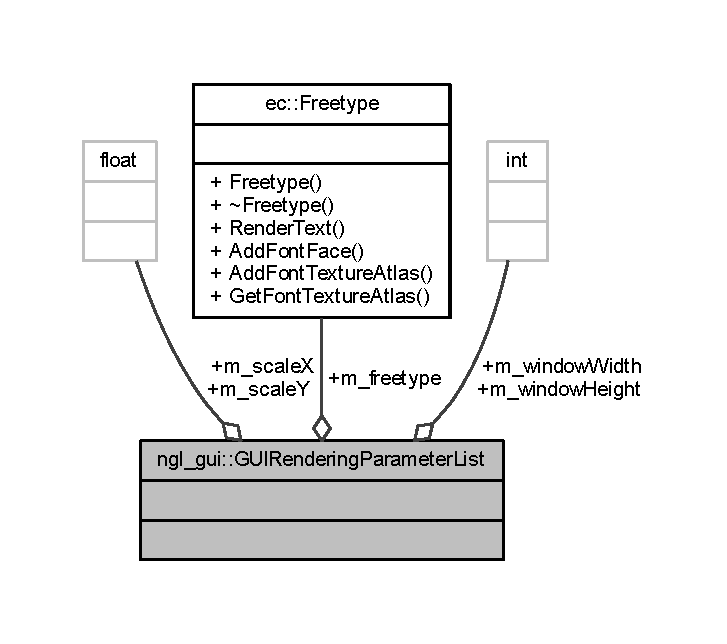
\includegraphics[width=349pt]{structngl__gui_1_1_g_u_i_rendering_parameter_list__coll__graph}
\end{center}
\end{figure}
\subsection*{Public Attributes}
\begin{DoxyCompactItemize}
\item 
\mbox{\hyperlink{classec_1_1_freetype}{ec\+::\+Freetype}} $\ast$ \mbox{\hyperlink{structngl__gui_1_1_g_u_i_rendering_parameter_list_a7613842cdc4f58969a2e913a0fa2bda0}{m\+\_\+freetype}}
\item 
float \mbox{\hyperlink{structngl__gui_1_1_g_u_i_rendering_parameter_list_a66e96c2c30bab54cb1e0c0b5fb79f0a0}{m\+\_\+scaleX}}
\item 
float \mbox{\hyperlink{structngl__gui_1_1_g_u_i_rendering_parameter_list_a3414b58859bb05449327f17bfc39dfca}{m\+\_\+scaleY}}
\item 
int \mbox{\hyperlink{structngl__gui_1_1_g_u_i_rendering_parameter_list_a57d3c0a09ed6c8b5d18472754024f6b6}{m\+\_\+window\+Width}}
\item 
int \mbox{\hyperlink{structngl__gui_1_1_g_u_i_rendering_parameter_list_acd396e477c473b4edf181953eb791639}{m\+\_\+window\+Height}}
\end{DoxyCompactItemize}


\subsection{Member Data Documentation}
\mbox{\Hypertarget{structngl__gui_1_1_g_u_i_rendering_parameter_list_a7613842cdc4f58969a2e913a0fa2bda0}\label{structngl__gui_1_1_g_u_i_rendering_parameter_list_a7613842cdc4f58969a2e913a0fa2bda0}} 
\index{ngl\+\_\+gui\+::\+G\+U\+I\+Rendering\+Parameter\+List@{ngl\+\_\+gui\+::\+G\+U\+I\+Rendering\+Parameter\+List}!m\+\_\+freetype@{m\+\_\+freetype}}
\index{m\+\_\+freetype@{m\+\_\+freetype}!ngl\+\_\+gui\+::\+G\+U\+I\+Rendering\+Parameter\+List@{ngl\+\_\+gui\+::\+G\+U\+I\+Rendering\+Parameter\+List}}
\subsubsection{\texorpdfstring{m\+\_\+freetype}{m\_freetype}}
{\footnotesize\ttfamily \mbox{\hyperlink{classec_1_1_freetype}{ec\+::\+Freetype}}$\ast$ ngl\+\_\+gui\+::\+G\+U\+I\+Rendering\+Parameter\+List\+::m\+\_\+freetype}

\mbox{\Hypertarget{structngl__gui_1_1_g_u_i_rendering_parameter_list_a66e96c2c30bab54cb1e0c0b5fb79f0a0}\label{structngl__gui_1_1_g_u_i_rendering_parameter_list_a66e96c2c30bab54cb1e0c0b5fb79f0a0}} 
\index{ngl\+\_\+gui\+::\+G\+U\+I\+Rendering\+Parameter\+List@{ngl\+\_\+gui\+::\+G\+U\+I\+Rendering\+Parameter\+List}!m\+\_\+scaleX@{m\+\_\+scaleX}}
\index{m\+\_\+scaleX@{m\+\_\+scaleX}!ngl\+\_\+gui\+::\+G\+U\+I\+Rendering\+Parameter\+List@{ngl\+\_\+gui\+::\+G\+U\+I\+Rendering\+Parameter\+List}}
\subsubsection{\texorpdfstring{m\+\_\+scaleX}{m\_scaleX}}
{\footnotesize\ttfamily float ngl\+\_\+gui\+::\+G\+U\+I\+Rendering\+Parameter\+List\+::m\+\_\+scaleX}

\mbox{\Hypertarget{structngl__gui_1_1_g_u_i_rendering_parameter_list_a3414b58859bb05449327f17bfc39dfca}\label{structngl__gui_1_1_g_u_i_rendering_parameter_list_a3414b58859bb05449327f17bfc39dfca}} 
\index{ngl\+\_\+gui\+::\+G\+U\+I\+Rendering\+Parameter\+List@{ngl\+\_\+gui\+::\+G\+U\+I\+Rendering\+Parameter\+List}!m\+\_\+scaleY@{m\+\_\+scaleY}}
\index{m\+\_\+scaleY@{m\+\_\+scaleY}!ngl\+\_\+gui\+::\+G\+U\+I\+Rendering\+Parameter\+List@{ngl\+\_\+gui\+::\+G\+U\+I\+Rendering\+Parameter\+List}}
\subsubsection{\texorpdfstring{m\+\_\+scaleY}{m\_scaleY}}
{\footnotesize\ttfamily float ngl\+\_\+gui\+::\+G\+U\+I\+Rendering\+Parameter\+List\+::m\+\_\+scaleY}

\mbox{\Hypertarget{structngl__gui_1_1_g_u_i_rendering_parameter_list_acd396e477c473b4edf181953eb791639}\label{structngl__gui_1_1_g_u_i_rendering_parameter_list_acd396e477c473b4edf181953eb791639}} 
\index{ngl\+\_\+gui\+::\+G\+U\+I\+Rendering\+Parameter\+List@{ngl\+\_\+gui\+::\+G\+U\+I\+Rendering\+Parameter\+List}!m\+\_\+window\+Height@{m\+\_\+window\+Height}}
\index{m\+\_\+window\+Height@{m\+\_\+window\+Height}!ngl\+\_\+gui\+::\+G\+U\+I\+Rendering\+Parameter\+List@{ngl\+\_\+gui\+::\+G\+U\+I\+Rendering\+Parameter\+List}}
\subsubsection{\texorpdfstring{m\+\_\+window\+Height}{m\_windowHeight}}
{\footnotesize\ttfamily int ngl\+\_\+gui\+::\+G\+U\+I\+Rendering\+Parameter\+List\+::m\+\_\+window\+Height}

\mbox{\Hypertarget{structngl__gui_1_1_g_u_i_rendering_parameter_list_a57d3c0a09ed6c8b5d18472754024f6b6}\label{structngl__gui_1_1_g_u_i_rendering_parameter_list_a57d3c0a09ed6c8b5d18472754024f6b6}} 
\index{ngl\+\_\+gui\+::\+G\+U\+I\+Rendering\+Parameter\+List@{ngl\+\_\+gui\+::\+G\+U\+I\+Rendering\+Parameter\+List}!m\+\_\+window\+Width@{m\+\_\+window\+Width}}
\index{m\+\_\+window\+Width@{m\+\_\+window\+Width}!ngl\+\_\+gui\+::\+G\+U\+I\+Rendering\+Parameter\+List@{ngl\+\_\+gui\+::\+G\+U\+I\+Rendering\+Parameter\+List}}
\subsubsection{\texorpdfstring{m\+\_\+window\+Width}{m\_windowWidth}}
{\footnotesize\ttfamily int ngl\+\_\+gui\+::\+G\+U\+I\+Rendering\+Parameter\+List\+::m\+\_\+window\+Width}



The documentation for this struct was generated from the following file\+:\begin{DoxyCompactItemize}
\item 
D\+:/\+Library/\+Documents/\+Job/\+Forschungsmaster/\+Projekte/\+Eye\+Candy3\+D/\+Eye\+Candy3\+D/include/\+E\+C3\+D/\+G\+U\+I/\mbox{\hyperlink{_g_u_i_renderer_8h}{G\+U\+I\+Renderer.\+h}}\end{DoxyCompactItemize}

\hypertarget{classngl__gui_1_1_g_u_i_system}{}\section{ngl\+\_\+gui\+:\+:G\+U\+I\+System Class Reference}
\label{classngl__gui_1_1_g_u_i_system}\index{ngl\+\_\+gui\+::\+G\+U\+I\+System@{ngl\+\_\+gui\+::\+G\+U\+I\+System}}


{\ttfamily \#include $<$G\+U\+I\+System.\+h$>$}



Collaboration diagram for ngl\+\_\+gui\+:\+:G\+U\+I\+System\+:\nopagebreak
\begin{figure}[H]
\begin{center}
\leavevmode
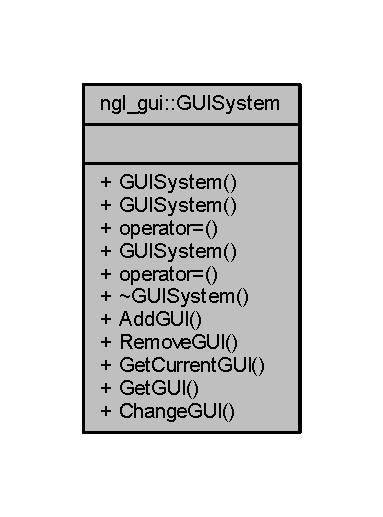
\includegraphics[width=184pt]{classngl__gui_1_1_g_u_i_system__coll__graph}
\end{center}
\end{figure}
\subsection*{Public Member Functions}
\begin{DoxyCompactItemize}
\item 
\mbox{\hyperlink{classngl__gui_1_1_g_u_i_system_ae3b077b89c26ad3b6fdc3f6552d7508e}{G\+U\+I\+System}} ()
\item 
\mbox{\hyperlink{classngl__gui_1_1_g_u_i_system_afc422ee53a06e72b1faf11df5f723792}{G\+U\+I\+System}} (const \mbox{\hyperlink{classngl__gui_1_1_g_u_i_system}{G\+U\+I\+System}} \&gui\+System)=delete
\item 
\mbox{\hyperlink{classngl__gui_1_1_g_u_i_system}{G\+U\+I\+System}} \& \mbox{\hyperlink{classngl__gui_1_1_g_u_i_system_a72358aba320d94377b8c2dfbdb7a78bc}{operator=}} (const \mbox{\hyperlink{classngl__gui_1_1_g_u_i_system}{G\+U\+I\+System}} \&gui\+System)=delete
\item 
\mbox{\hyperlink{classngl__gui_1_1_g_u_i_system_add8945f8c4a203128ff35878d3e9447b}{G\+U\+I\+System}} (\mbox{\hyperlink{classngl__gui_1_1_g_u_i_system}{G\+U\+I\+System}} \&\&gui\+System)=default
\item 
\mbox{\hyperlink{classngl__gui_1_1_g_u_i_system}{G\+U\+I\+System}} \& \mbox{\hyperlink{classngl__gui_1_1_g_u_i_system_a7d917255efcdbf070857f4c9846646d2}{operator=}} (\mbox{\hyperlink{classngl__gui_1_1_g_u_i_system}{G\+U\+I\+System}} \&\&gui\+System)=default
\item 
\mbox{\hyperlink{classngl__gui_1_1_g_u_i_system_aea572afaf1840acb0da5da07a1eb551b}{$\sim$\+G\+U\+I\+System}} ()
\item 
void \mbox{\hyperlink{classngl__gui_1_1_g_u_i_system_a4743d6da816cae8e319fe9351854731f}{Add\+G\+UI}} (\mbox{\hyperlink{classngl__gui_1_1_g_u_i}{G\+UI}} $\ast$gui)
\item 
bool \mbox{\hyperlink{classngl__gui_1_1_g_u_i_system_a5d826ebd83f05e1332cd9737fc43ecd3}{Remove\+G\+UI}} (\mbox{\hyperlink{classngl__gui_1_1_g_u_i}{G\+UI}} $\ast$gui)
\item 
\mbox{\hyperlink{classngl__gui_1_1_g_u_i}{G\+UI}} $\ast$ \mbox{\hyperlink{classngl__gui_1_1_g_u_i_system_a81746712ea980afa64f95b630ee498d7}{Get\+Current\+G\+UI}} ()
\item 
\mbox{\hyperlink{classngl__gui_1_1_g_u_i}{G\+UI}} $\ast$ \mbox{\hyperlink{classngl__gui_1_1_g_u_i_system_adeb4564e37eb08d12419ee91cc6b2f89}{Get\+G\+UI}} (const std\+::string \&name)
\item 
bool \mbox{\hyperlink{classngl__gui_1_1_g_u_i_system_a437c1de904bcfd2427d062ad147dbacc}{Change\+G\+UI}} (const std\+::string \&gui\+Name)
\end{DoxyCompactItemize}


\subsection{Constructor \& Destructor Documentation}
\mbox{\Hypertarget{classngl__gui_1_1_g_u_i_system_ae3b077b89c26ad3b6fdc3f6552d7508e}\label{classngl__gui_1_1_g_u_i_system_ae3b077b89c26ad3b6fdc3f6552d7508e}} 
\index{ngl\+\_\+gui\+::\+G\+U\+I\+System@{ngl\+\_\+gui\+::\+G\+U\+I\+System}!G\+U\+I\+System@{G\+U\+I\+System}}
\index{G\+U\+I\+System@{G\+U\+I\+System}!ngl\+\_\+gui\+::\+G\+U\+I\+System@{ngl\+\_\+gui\+::\+G\+U\+I\+System}}
\subsubsection{\texorpdfstring{G\+U\+I\+System()}{GUISystem()}\hspace{0.1cm}{\footnotesize\ttfamily [1/3]}}
{\footnotesize\ttfamily ngl\+\_\+gui\+::\+G\+U\+I\+System\+::\+G\+U\+I\+System (\begin{DoxyParamCaption}{ }\end{DoxyParamCaption})\hspace{0.3cm}{\ttfamily [explicit]}}

\mbox{\Hypertarget{classngl__gui_1_1_g_u_i_system_afc422ee53a06e72b1faf11df5f723792}\label{classngl__gui_1_1_g_u_i_system_afc422ee53a06e72b1faf11df5f723792}} 
\index{ngl\+\_\+gui\+::\+G\+U\+I\+System@{ngl\+\_\+gui\+::\+G\+U\+I\+System}!G\+U\+I\+System@{G\+U\+I\+System}}
\index{G\+U\+I\+System@{G\+U\+I\+System}!ngl\+\_\+gui\+::\+G\+U\+I\+System@{ngl\+\_\+gui\+::\+G\+U\+I\+System}}
\subsubsection{\texorpdfstring{G\+U\+I\+System()}{GUISystem()}\hspace{0.1cm}{\footnotesize\ttfamily [2/3]}}
{\footnotesize\ttfamily ngl\+\_\+gui\+::\+G\+U\+I\+System\+::\+G\+U\+I\+System (\begin{DoxyParamCaption}\item[{const \mbox{\hyperlink{classngl__gui_1_1_g_u_i_system}{G\+U\+I\+System}} \&}]{gui\+System }\end{DoxyParamCaption})\hspace{0.3cm}{\ttfamily [delete]}}

\mbox{\Hypertarget{classngl__gui_1_1_g_u_i_system_add8945f8c4a203128ff35878d3e9447b}\label{classngl__gui_1_1_g_u_i_system_add8945f8c4a203128ff35878d3e9447b}} 
\index{ngl\+\_\+gui\+::\+G\+U\+I\+System@{ngl\+\_\+gui\+::\+G\+U\+I\+System}!G\+U\+I\+System@{G\+U\+I\+System}}
\index{G\+U\+I\+System@{G\+U\+I\+System}!ngl\+\_\+gui\+::\+G\+U\+I\+System@{ngl\+\_\+gui\+::\+G\+U\+I\+System}}
\subsubsection{\texorpdfstring{G\+U\+I\+System()}{GUISystem()}\hspace{0.1cm}{\footnotesize\ttfamily [3/3]}}
{\footnotesize\ttfamily ngl\+\_\+gui\+::\+G\+U\+I\+System\+::\+G\+U\+I\+System (\begin{DoxyParamCaption}\item[{\mbox{\hyperlink{classngl__gui_1_1_g_u_i_system}{G\+U\+I\+System}} \&\&}]{gui\+System }\end{DoxyParamCaption})\hspace{0.3cm}{\ttfamily [default]}}

\mbox{\Hypertarget{classngl__gui_1_1_g_u_i_system_aea572afaf1840acb0da5da07a1eb551b}\label{classngl__gui_1_1_g_u_i_system_aea572afaf1840acb0da5da07a1eb551b}} 
\index{ngl\+\_\+gui\+::\+G\+U\+I\+System@{ngl\+\_\+gui\+::\+G\+U\+I\+System}!````~G\+U\+I\+System@{$\sim$\+G\+U\+I\+System}}
\index{````~G\+U\+I\+System@{$\sim$\+G\+U\+I\+System}!ngl\+\_\+gui\+::\+G\+U\+I\+System@{ngl\+\_\+gui\+::\+G\+U\+I\+System}}
\subsubsection{\texorpdfstring{$\sim$\+G\+U\+I\+System()}{~GUISystem()}}
{\footnotesize\ttfamily ngl\+\_\+gui\+::\+G\+U\+I\+System\+::$\sim$\+G\+U\+I\+System (\begin{DoxyParamCaption}{ }\end{DoxyParamCaption})}



\subsection{Member Function Documentation}
\mbox{\Hypertarget{classngl__gui_1_1_g_u_i_system_a4743d6da816cae8e319fe9351854731f}\label{classngl__gui_1_1_g_u_i_system_a4743d6da816cae8e319fe9351854731f}} 
\index{ngl\+\_\+gui\+::\+G\+U\+I\+System@{ngl\+\_\+gui\+::\+G\+U\+I\+System}!Add\+G\+UI@{Add\+G\+UI}}
\index{Add\+G\+UI@{Add\+G\+UI}!ngl\+\_\+gui\+::\+G\+U\+I\+System@{ngl\+\_\+gui\+::\+G\+U\+I\+System}}
\subsubsection{\texorpdfstring{Add\+G\+U\+I()}{AddGUI()}}
{\footnotesize\ttfamily void ngl\+\_\+gui\+::\+G\+U\+I\+System\+::\+Add\+G\+UI (\begin{DoxyParamCaption}\item[{\mbox{\hyperlink{classngl__gui_1_1_g_u_i}{G\+UI}} $\ast$}]{gui }\end{DoxyParamCaption})}

\mbox{\Hypertarget{classngl__gui_1_1_g_u_i_system_a437c1de904bcfd2427d062ad147dbacc}\label{classngl__gui_1_1_g_u_i_system_a437c1de904bcfd2427d062ad147dbacc}} 
\index{ngl\+\_\+gui\+::\+G\+U\+I\+System@{ngl\+\_\+gui\+::\+G\+U\+I\+System}!Change\+G\+UI@{Change\+G\+UI}}
\index{Change\+G\+UI@{Change\+G\+UI}!ngl\+\_\+gui\+::\+G\+U\+I\+System@{ngl\+\_\+gui\+::\+G\+U\+I\+System}}
\subsubsection{\texorpdfstring{Change\+G\+U\+I()}{ChangeGUI()}}
{\footnotesize\ttfamily bool ngl\+\_\+gui\+::\+G\+U\+I\+System\+::\+Change\+G\+UI (\begin{DoxyParamCaption}\item[{const std\+::string \&}]{gui\+Name }\end{DoxyParamCaption})}

\mbox{\Hypertarget{classngl__gui_1_1_g_u_i_system_a81746712ea980afa64f95b630ee498d7}\label{classngl__gui_1_1_g_u_i_system_a81746712ea980afa64f95b630ee498d7}} 
\index{ngl\+\_\+gui\+::\+G\+U\+I\+System@{ngl\+\_\+gui\+::\+G\+U\+I\+System}!Get\+Current\+G\+UI@{Get\+Current\+G\+UI}}
\index{Get\+Current\+G\+UI@{Get\+Current\+G\+UI}!ngl\+\_\+gui\+::\+G\+U\+I\+System@{ngl\+\_\+gui\+::\+G\+U\+I\+System}}
\subsubsection{\texorpdfstring{Get\+Current\+G\+U\+I()}{GetCurrentGUI()}}
{\footnotesize\ttfamily \mbox{\hyperlink{classngl__gui_1_1_g_u_i}{ngl\+\_\+gui\+::\+G\+UI}} $\ast$ ngl\+\_\+gui\+::\+G\+U\+I\+System\+::\+Get\+Current\+G\+UI (\begin{DoxyParamCaption}{ }\end{DoxyParamCaption})}

\mbox{\Hypertarget{classngl__gui_1_1_g_u_i_system_adeb4564e37eb08d12419ee91cc6b2f89}\label{classngl__gui_1_1_g_u_i_system_adeb4564e37eb08d12419ee91cc6b2f89}} 
\index{ngl\+\_\+gui\+::\+G\+U\+I\+System@{ngl\+\_\+gui\+::\+G\+U\+I\+System}!Get\+G\+UI@{Get\+G\+UI}}
\index{Get\+G\+UI@{Get\+G\+UI}!ngl\+\_\+gui\+::\+G\+U\+I\+System@{ngl\+\_\+gui\+::\+G\+U\+I\+System}}
\subsubsection{\texorpdfstring{Get\+G\+U\+I()}{GetGUI()}}
{\footnotesize\ttfamily \mbox{\hyperlink{classngl__gui_1_1_g_u_i}{ngl\+\_\+gui\+::\+G\+UI}} $\ast$ ngl\+\_\+gui\+::\+G\+U\+I\+System\+::\+Get\+G\+UI (\begin{DoxyParamCaption}\item[{const std\+::string \&}]{name }\end{DoxyParamCaption})}

\mbox{\Hypertarget{classngl__gui_1_1_g_u_i_system_a72358aba320d94377b8c2dfbdb7a78bc}\label{classngl__gui_1_1_g_u_i_system_a72358aba320d94377b8c2dfbdb7a78bc}} 
\index{ngl\+\_\+gui\+::\+G\+U\+I\+System@{ngl\+\_\+gui\+::\+G\+U\+I\+System}!operator=@{operator=}}
\index{operator=@{operator=}!ngl\+\_\+gui\+::\+G\+U\+I\+System@{ngl\+\_\+gui\+::\+G\+U\+I\+System}}
\subsubsection{\texorpdfstring{operator=()}{operator=()}\hspace{0.1cm}{\footnotesize\ttfamily [1/2]}}
{\footnotesize\ttfamily \mbox{\hyperlink{classngl__gui_1_1_g_u_i_system}{G\+U\+I\+System}}\& ngl\+\_\+gui\+::\+G\+U\+I\+System\+::operator= (\begin{DoxyParamCaption}\item[{const \mbox{\hyperlink{classngl__gui_1_1_g_u_i_system}{G\+U\+I\+System}} \&}]{gui\+System }\end{DoxyParamCaption})\hspace{0.3cm}{\ttfamily [delete]}}

\mbox{\Hypertarget{classngl__gui_1_1_g_u_i_system_a7d917255efcdbf070857f4c9846646d2}\label{classngl__gui_1_1_g_u_i_system_a7d917255efcdbf070857f4c9846646d2}} 
\index{ngl\+\_\+gui\+::\+G\+U\+I\+System@{ngl\+\_\+gui\+::\+G\+U\+I\+System}!operator=@{operator=}}
\index{operator=@{operator=}!ngl\+\_\+gui\+::\+G\+U\+I\+System@{ngl\+\_\+gui\+::\+G\+U\+I\+System}}
\subsubsection{\texorpdfstring{operator=()}{operator=()}\hspace{0.1cm}{\footnotesize\ttfamily [2/2]}}
{\footnotesize\ttfamily \mbox{\hyperlink{classngl__gui_1_1_g_u_i_system}{G\+U\+I\+System}}\& ngl\+\_\+gui\+::\+G\+U\+I\+System\+::operator= (\begin{DoxyParamCaption}\item[{\mbox{\hyperlink{classngl__gui_1_1_g_u_i_system}{G\+U\+I\+System}} \&\&}]{gui\+System }\end{DoxyParamCaption})\hspace{0.3cm}{\ttfamily [default]}}

\mbox{\Hypertarget{classngl__gui_1_1_g_u_i_system_a5d826ebd83f05e1332cd9737fc43ecd3}\label{classngl__gui_1_1_g_u_i_system_a5d826ebd83f05e1332cd9737fc43ecd3}} 
\index{ngl\+\_\+gui\+::\+G\+U\+I\+System@{ngl\+\_\+gui\+::\+G\+U\+I\+System}!Remove\+G\+UI@{Remove\+G\+UI}}
\index{Remove\+G\+UI@{Remove\+G\+UI}!ngl\+\_\+gui\+::\+G\+U\+I\+System@{ngl\+\_\+gui\+::\+G\+U\+I\+System}}
\subsubsection{\texorpdfstring{Remove\+G\+U\+I()}{RemoveGUI()}}
{\footnotesize\ttfamily bool ngl\+\_\+gui\+::\+G\+U\+I\+System\+::\+Remove\+G\+UI (\begin{DoxyParamCaption}\item[{\mbox{\hyperlink{classngl__gui_1_1_g_u_i}{G\+UI}} $\ast$}]{gui }\end{DoxyParamCaption})}



The documentation for this class was generated from the following files\+:\begin{DoxyCompactItemize}
\item 
D\+:/\+Library/\+Documents/\+Job/\+Forschungsmaster/\+Projekte/\+Eye\+Candy3\+D/\+Eye\+Candy3\+D/include/\+E\+C3\+D/\+G\+U\+I/\mbox{\hyperlink{_g_u_i_system_8h}{G\+U\+I\+System.\+h}}\item 
D\+:/\+Library/\+Documents/\+Job/\+Forschungsmaster/\+Projekte/\+Eye\+Candy3\+D/\+Eye\+Candy3\+D/src/\+G\+U\+I/\mbox{\hyperlink{_g_u_i_system_8cpp}{G\+U\+I\+System.\+cpp}}\end{DoxyCompactItemize}

\hypertarget{classngl__gui_1_1_horizontal_list}{}\section{ngl\+\_\+gui\+:\+:Horizontal\+List Class Reference}
\label{classngl__gui_1_1_horizontal_list}\index{ngl\+\_\+gui\+::\+Horizontal\+List@{ngl\+\_\+gui\+::\+Horizontal\+List}}


{\ttfamily \#include $<$Horizontal\+List.\+h$>$}



Inheritance diagram for ngl\+\_\+gui\+:\+:Horizontal\+List\+:\nopagebreak
\begin{figure}[H]
\begin{center}
\leavevmode
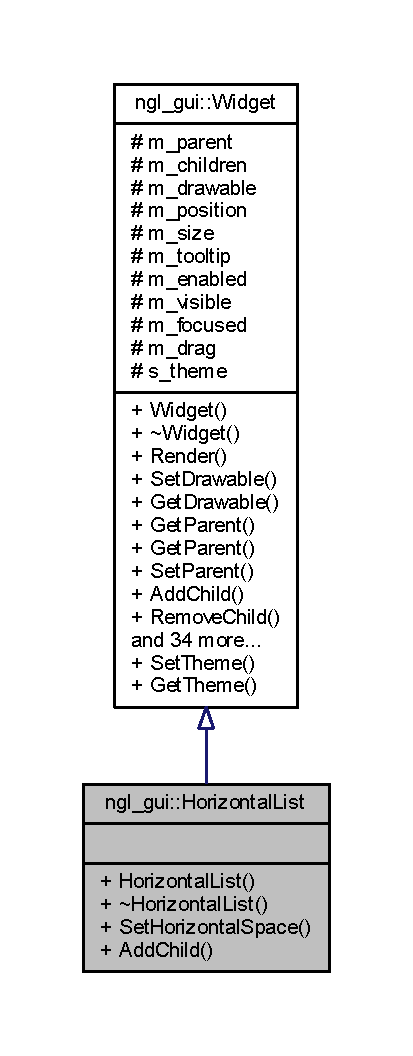
\includegraphics[width=198pt]{classngl__gui_1_1_horizontal_list__inherit__graph}
\end{center}
\end{figure}


Collaboration diagram for ngl\+\_\+gui\+:\+:Horizontal\+List\+:
\nopagebreak
\begin{figure}[H]
\begin{center}
\leavevmode
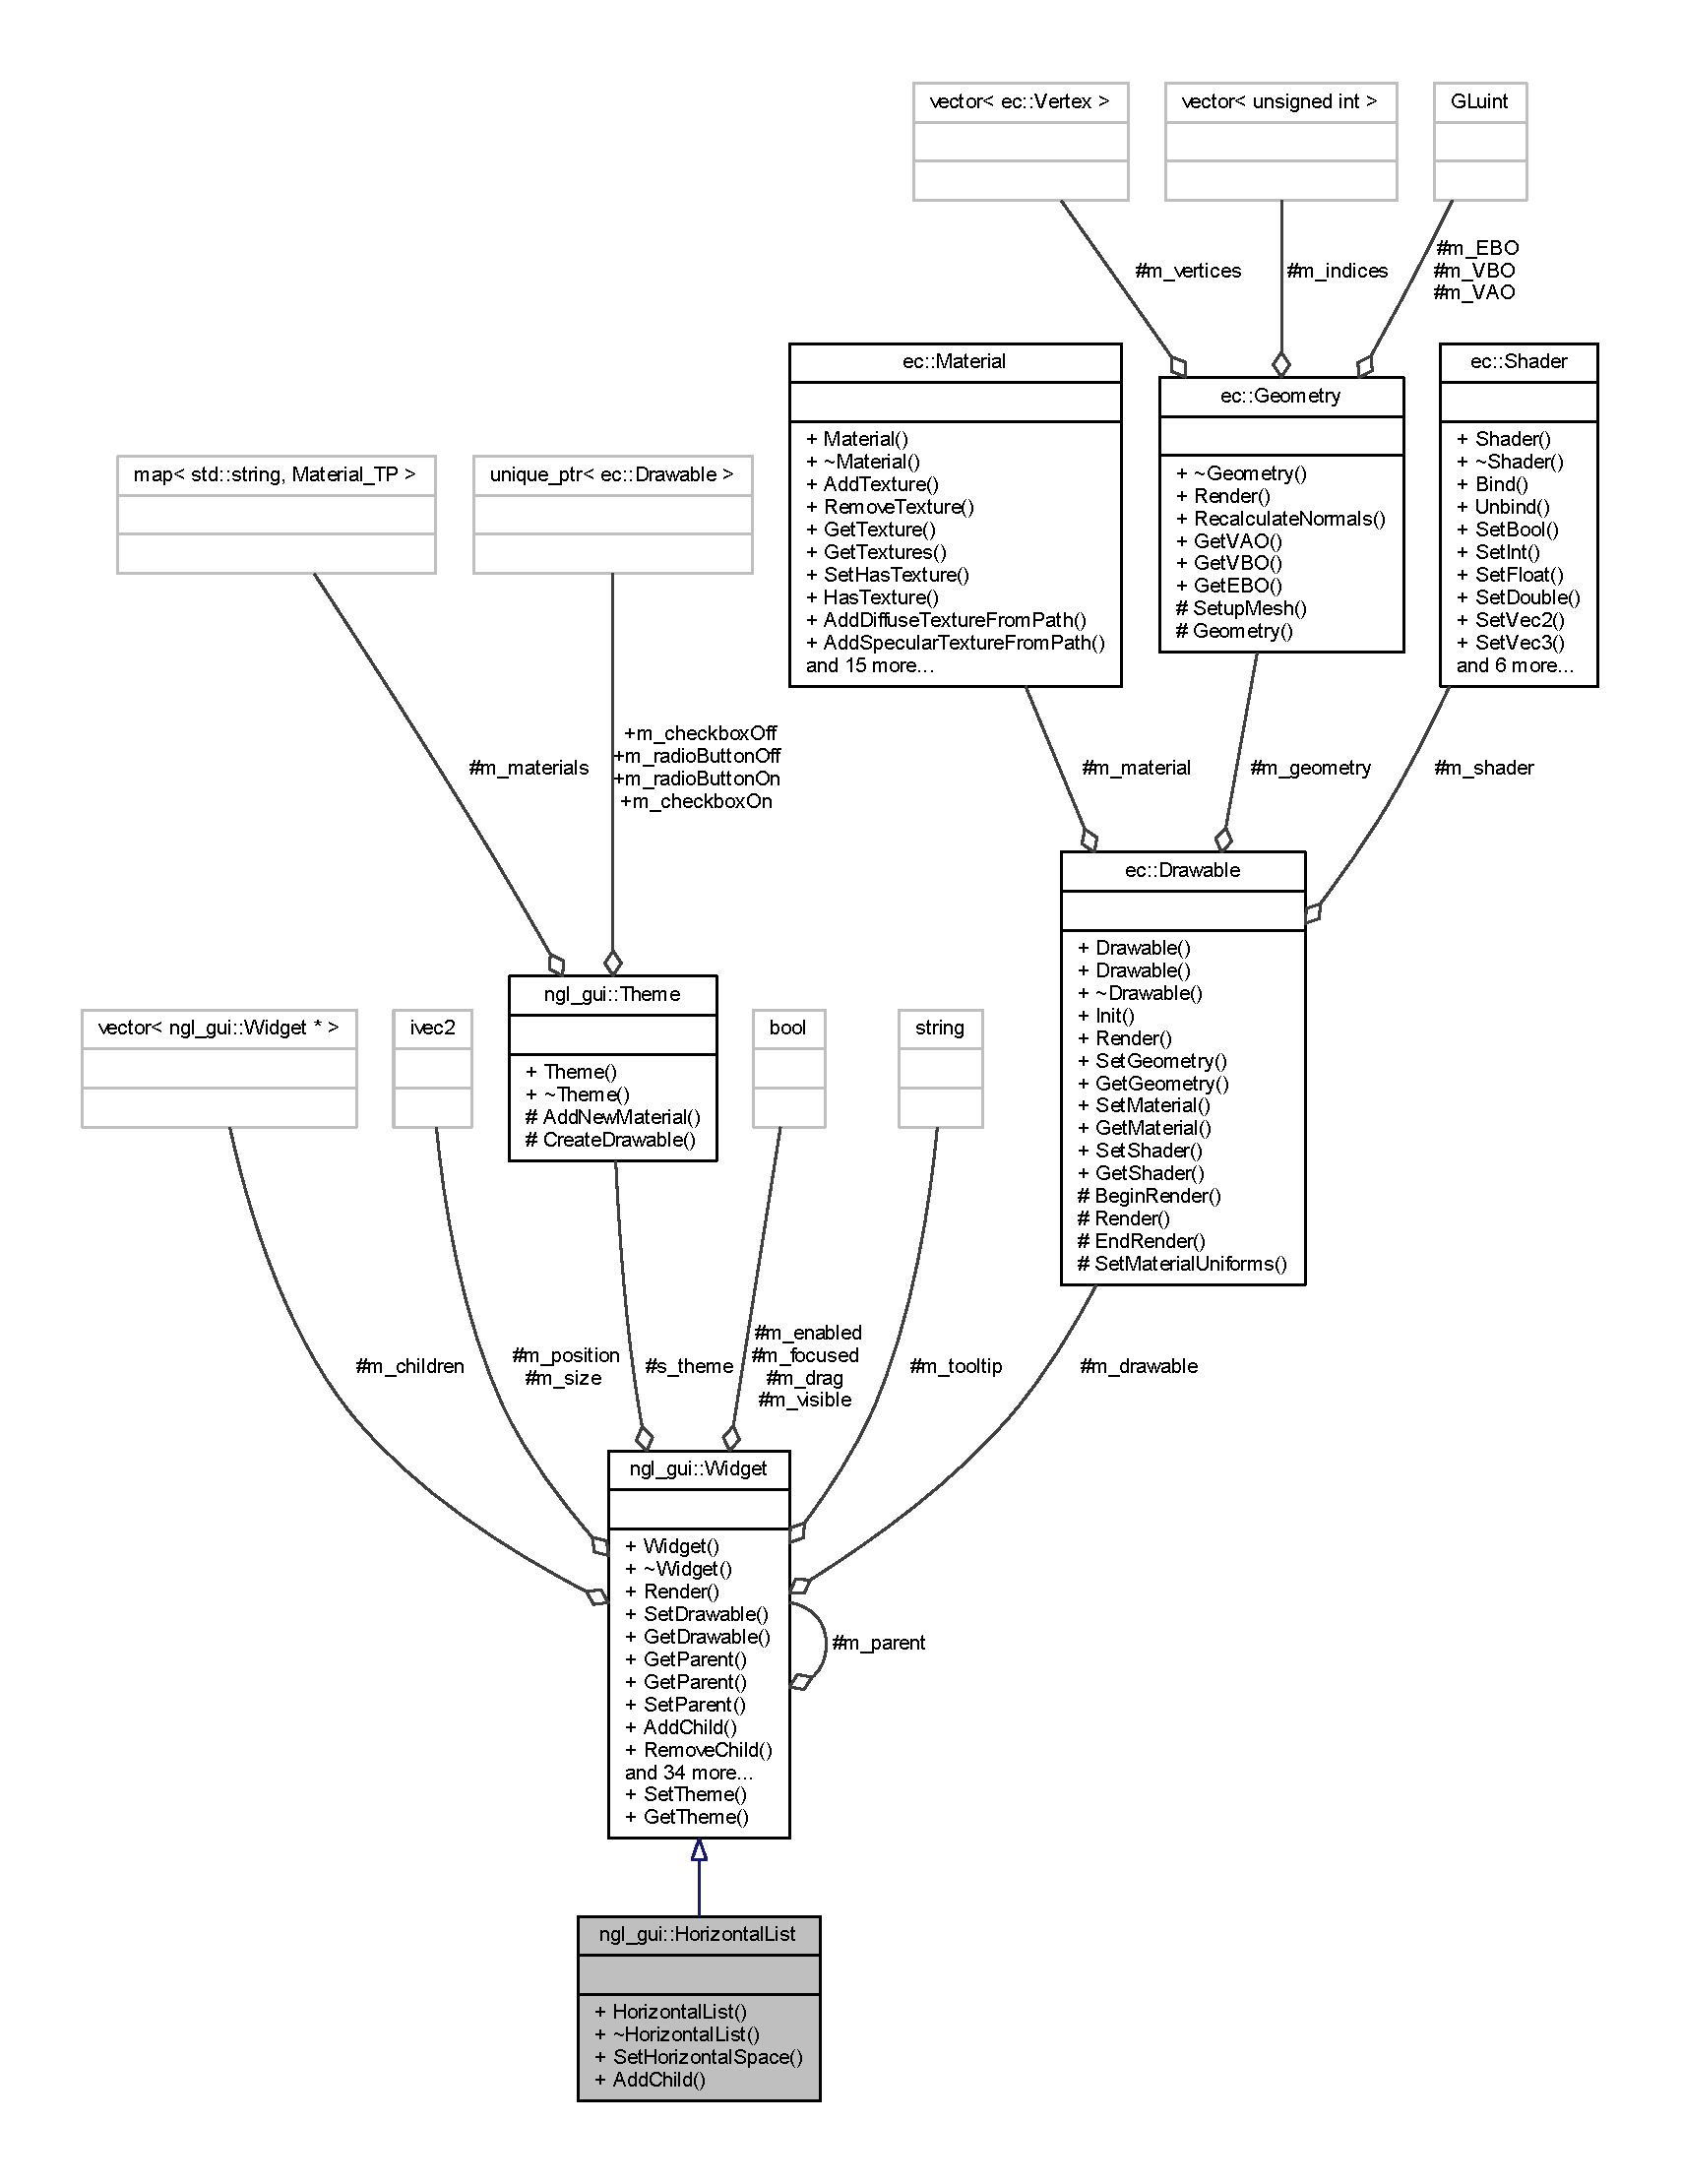
\includegraphics[width=350pt]{classngl__gui_1_1_horizontal_list__coll__graph}
\end{center}
\end{figure}
\subsection*{Public Member Functions}
\begin{DoxyCompactItemize}
\item 
\mbox{\hyperlink{classngl__gui_1_1_horizontal_list_a2b94e64efbf77b487aa08d49e23e1e41}{Horizontal\+List}} (\mbox{\hyperlink{classngl__gui_1_1_widget}{Widget}} $\ast$parent, int hspace=1)
\item 
\mbox{\hyperlink{classngl__gui_1_1_horizontal_list_a91fa289dccfaadf3dd043b1e945b18e6}{$\sim$\+Horizontal\+List}} ()
\item 
void \mbox{\hyperlink{classngl__gui_1_1_horizontal_list_affeae11b3f463f65d870938e525ab14d}{Set\+Horizontal\+Space}} (int hspace)
\item 
virtual void \mbox{\hyperlink{classngl__gui_1_1_horizontal_list_a3dcb8fc4e780268899d12ecc3980bc16}{Add\+Child}} (\mbox{\hyperlink{classngl__gui_1_1_widget}{Widget}} $\ast$widget) override
\end{DoxyCompactItemize}
\subsection*{Additional Inherited Members}


\subsection{Constructor \& Destructor Documentation}
\mbox{\Hypertarget{classngl__gui_1_1_horizontal_list_a2b94e64efbf77b487aa08d49e23e1e41}\label{classngl__gui_1_1_horizontal_list_a2b94e64efbf77b487aa08d49e23e1e41}} 
\index{ngl\+\_\+gui\+::\+Horizontal\+List@{ngl\+\_\+gui\+::\+Horizontal\+List}!Horizontal\+List@{Horizontal\+List}}
\index{Horizontal\+List@{Horizontal\+List}!ngl\+\_\+gui\+::\+Horizontal\+List@{ngl\+\_\+gui\+::\+Horizontal\+List}}
\subsubsection{\texorpdfstring{Horizontal\+List()}{HorizontalList()}}
{\footnotesize\ttfamily ngl\+\_\+gui\+::\+Horizontal\+List\+::\+Horizontal\+List (\begin{DoxyParamCaption}\item[{\mbox{\hyperlink{classngl__gui_1_1_widget}{Widget}} $\ast$}]{parent,  }\item[{int}]{hspace = {\ttfamily 1} }\end{DoxyParamCaption})\hspace{0.3cm}{\ttfamily [explicit]}}

\mbox{\Hypertarget{classngl__gui_1_1_horizontal_list_a91fa289dccfaadf3dd043b1e945b18e6}\label{classngl__gui_1_1_horizontal_list_a91fa289dccfaadf3dd043b1e945b18e6}} 
\index{ngl\+\_\+gui\+::\+Horizontal\+List@{ngl\+\_\+gui\+::\+Horizontal\+List}!````~Horizontal\+List@{$\sim$\+Horizontal\+List}}
\index{````~Horizontal\+List@{$\sim$\+Horizontal\+List}!ngl\+\_\+gui\+::\+Horizontal\+List@{ngl\+\_\+gui\+::\+Horizontal\+List}}
\subsubsection{\texorpdfstring{$\sim$\+Horizontal\+List()}{~HorizontalList()}}
{\footnotesize\ttfamily ngl\+\_\+gui\+::\+Horizontal\+List\+::$\sim$\+Horizontal\+List (\begin{DoxyParamCaption}{ }\end{DoxyParamCaption})}



\subsection{Member Function Documentation}
\mbox{\Hypertarget{classngl__gui_1_1_horizontal_list_a3dcb8fc4e780268899d12ecc3980bc16}\label{classngl__gui_1_1_horizontal_list_a3dcb8fc4e780268899d12ecc3980bc16}} 
\index{ngl\+\_\+gui\+::\+Horizontal\+List@{ngl\+\_\+gui\+::\+Horizontal\+List}!Add\+Child@{Add\+Child}}
\index{Add\+Child@{Add\+Child}!ngl\+\_\+gui\+::\+Horizontal\+List@{ngl\+\_\+gui\+::\+Horizontal\+List}}
\subsubsection{\texorpdfstring{Add\+Child()}{AddChild()}}
{\footnotesize\ttfamily void ngl\+\_\+gui\+::\+Horizontal\+List\+::\+Add\+Child (\begin{DoxyParamCaption}\item[{\mbox{\hyperlink{classngl__gui_1_1_widget}{Widget}} $\ast$}]{widget }\end{DoxyParamCaption})\hspace{0.3cm}{\ttfamily [override]}, {\ttfamily [virtual]}}



Reimplemented from \mbox{\hyperlink{classngl__gui_1_1_widget_a37128e55931fa4fe2f99556d4a45607a}{ngl\+\_\+gui\+::\+Widget}}.

\mbox{\Hypertarget{classngl__gui_1_1_horizontal_list_affeae11b3f463f65d870938e525ab14d}\label{classngl__gui_1_1_horizontal_list_affeae11b3f463f65d870938e525ab14d}} 
\index{ngl\+\_\+gui\+::\+Horizontal\+List@{ngl\+\_\+gui\+::\+Horizontal\+List}!Set\+Horizontal\+Space@{Set\+Horizontal\+Space}}
\index{Set\+Horizontal\+Space@{Set\+Horizontal\+Space}!ngl\+\_\+gui\+::\+Horizontal\+List@{ngl\+\_\+gui\+::\+Horizontal\+List}}
\subsubsection{\texorpdfstring{Set\+Horizontal\+Space()}{SetHorizontalSpace()}}
{\footnotesize\ttfamily void ngl\+\_\+gui\+::\+Horizontal\+List\+::\+Set\+Horizontal\+Space (\begin{DoxyParamCaption}\item[{int}]{hspace }\end{DoxyParamCaption})}



The documentation for this class was generated from the following files\+:\begin{DoxyCompactItemize}
\item 
D\+:/\+Library/\+Documents/\+Job/\+Forschungsmaster/\+Projekte/\+Eye\+Candy3\+D/\+Eye\+Candy3\+D/include/\+E\+C3\+D/\+G\+U\+I/\mbox{\hyperlink{_horizontal_list_8h}{Horizontal\+List.\+h}}\item 
D\+:/\+Library/\+Documents/\+Job/\+Forschungsmaster/\+Projekte/\+Eye\+Candy3\+D/\+Eye\+Candy3\+D/src/\+G\+U\+I/\mbox{\hyperlink{_horizontal_list_8cpp}{Horizontal\+List.\+cpp}}\end{DoxyCompactItemize}

\hypertarget{structec_1_1_input_event}{}\section{ec\+:\+:Input\+Event Struct Reference}
\label{structec_1_1_input_event}\index{ec\+::\+Input\+Event@{ec\+::\+Input\+Event}}


{\ttfamily \#include $<$Input\+Event.\+h$>$}



Collaboration diagram for ec\+:\+:Input\+Event\+:\nopagebreak
\begin{figure}[H]
\begin{center}
\leavevmode
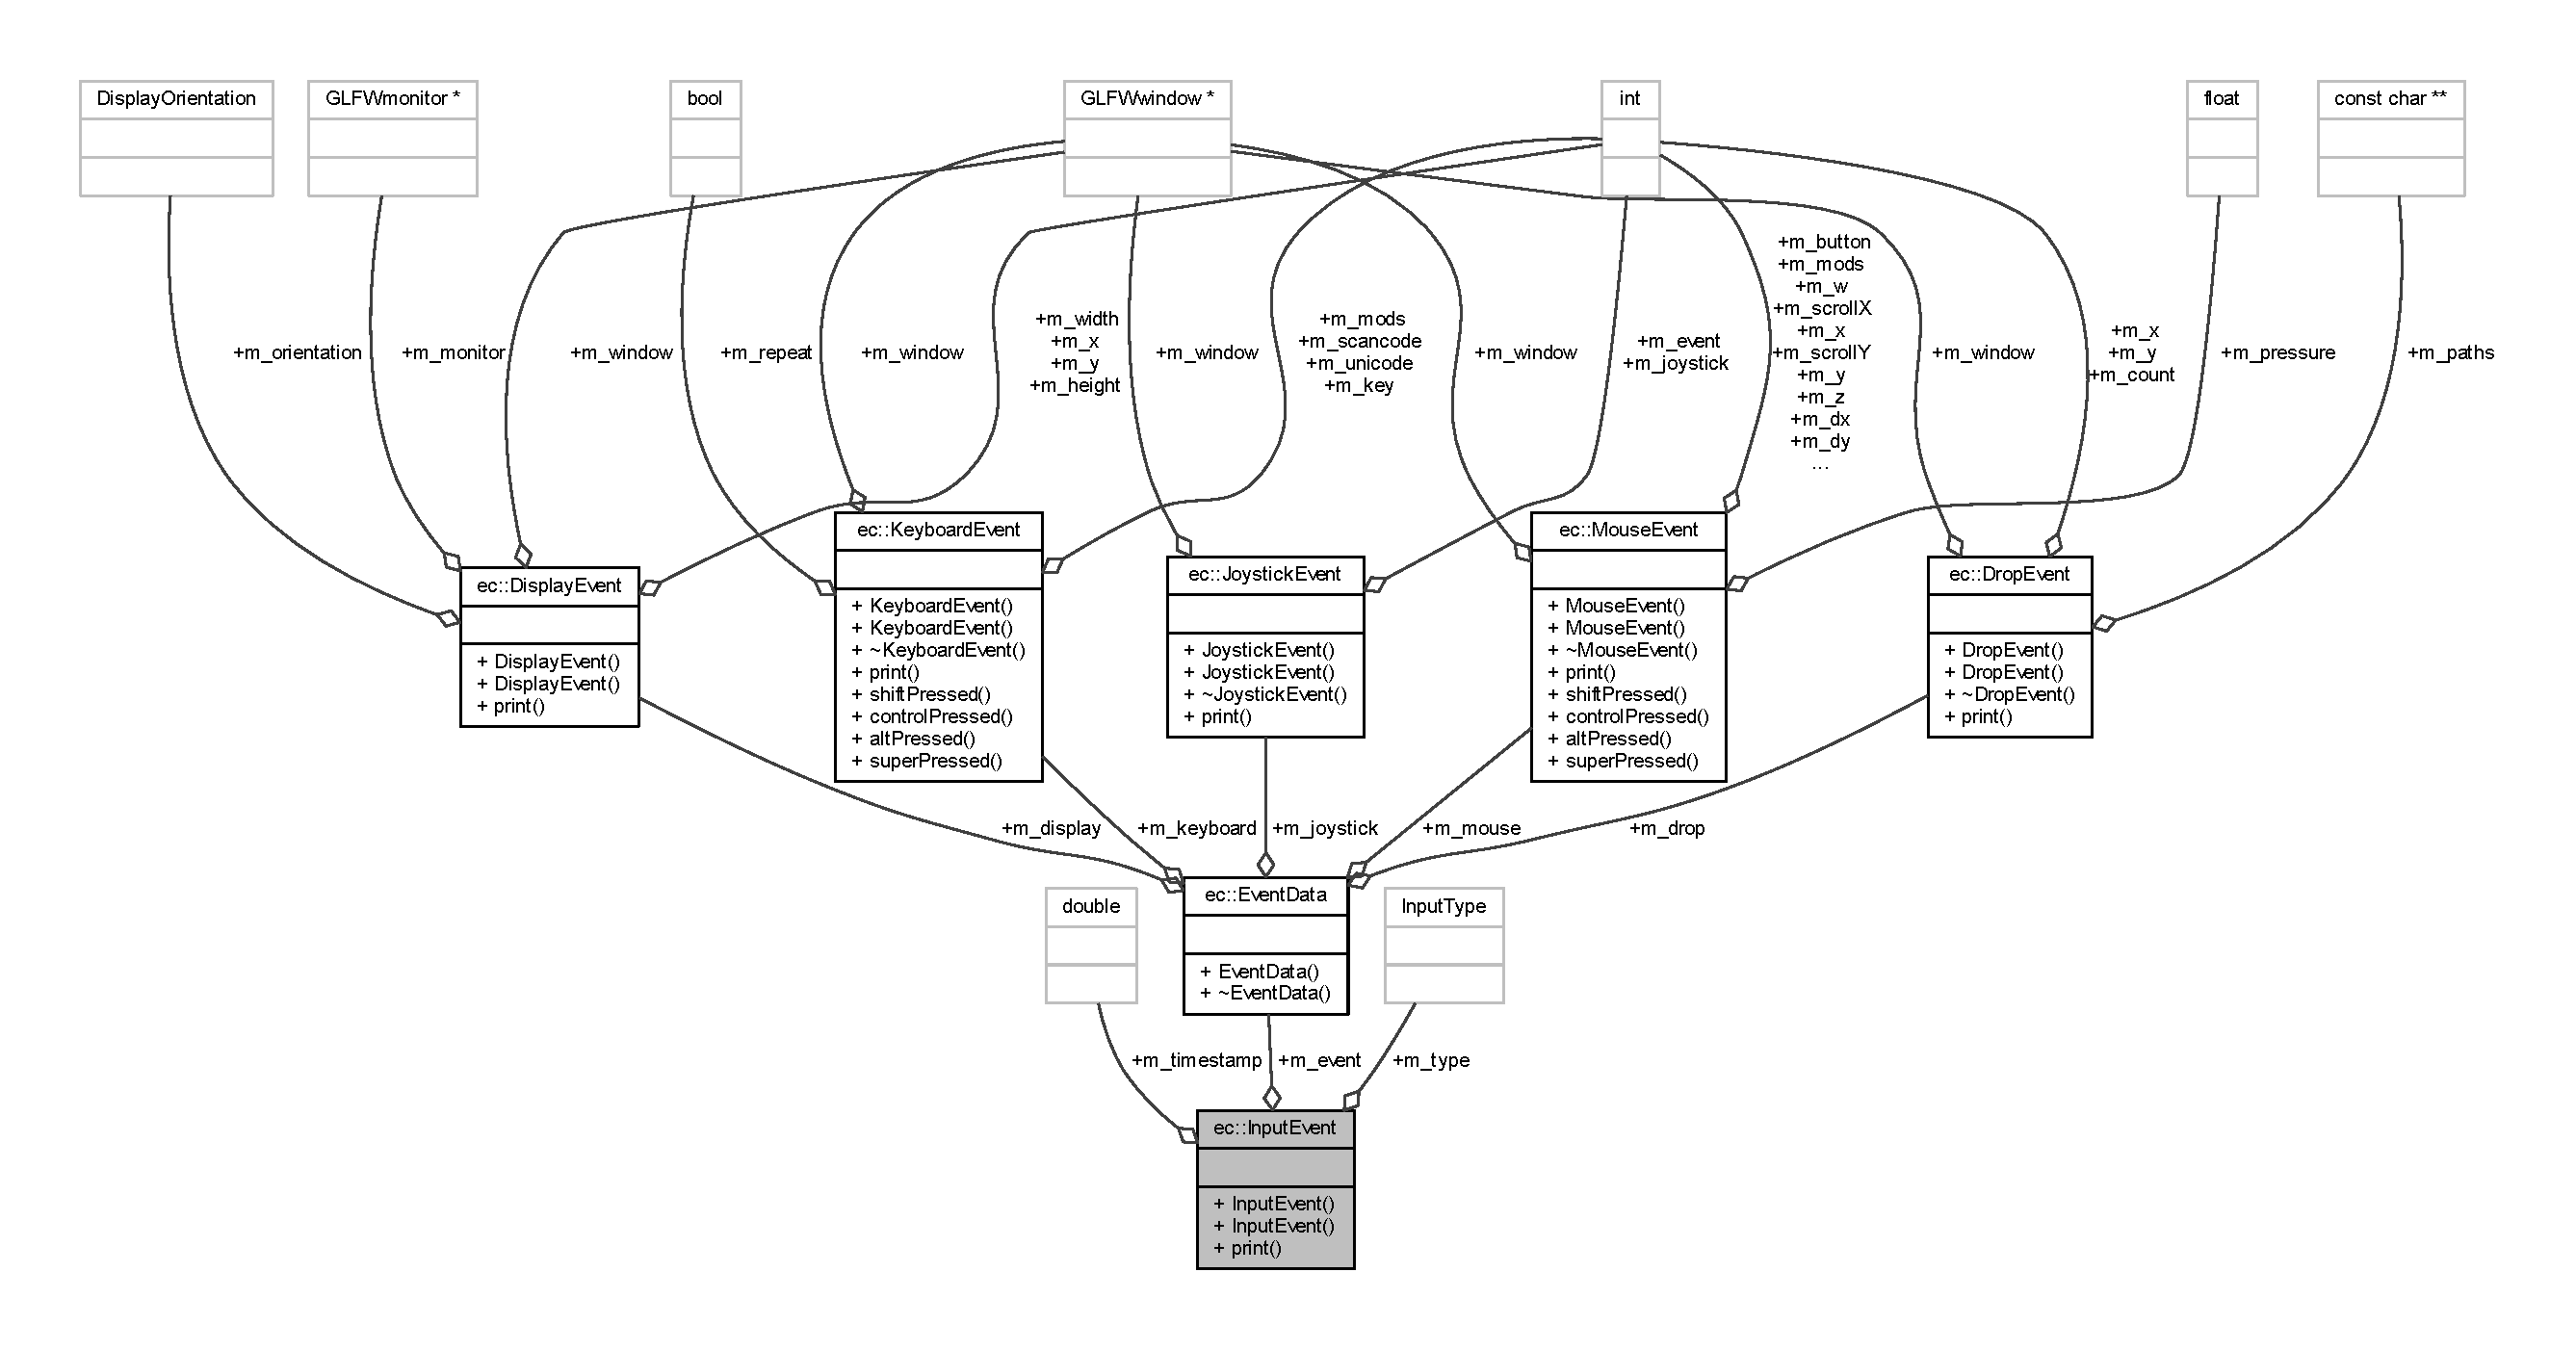
\includegraphics[width=350pt]{structec_1_1_input_event__coll__graph}
\end{center}
\end{figure}
\subsection*{Public Member Functions}
\begin{DoxyCompactItemize}
\item 
\mbox{\hyperlink{structec_1_1_input_event_a0e1dd98eb4e1161bdb573afe429d07c8}{Input\+Event}} ()
\item 
\mbox{\hyperlink{structec_1_1_input_event_af8894b724a61a63412f4e6df14a49d7a}{Input\+Event}} (\mbox{\hyperlink{namespaceec_a5de6bdb8c4b2ed6e590e721ec998f964}{Input\+Type}} type)
\item 
void \mbox{\hyperlink{structec_1_1_input_event_a778cd0afc60db1b127585a54c61b9e75}{print}} () const
\end{DoxyCompactItemize}
\subsection*{Public Attributes}
\begin{DoxyCompactItemize}
\item 
\mbox{\hyperlink{namespaceec_a5de6bdb8c4b2ed6e590e721ec998f964}{Input\+Type}} \mbox{\hyperlink{structec_1_1_input_event_a07aadaf18da2952478b803bbd4122bb7}{m\+\_\+type}}
\item 
double \mbox{\hyperlink{structec_1_1_input_event_ada54908facf585cb714bd6712d8f6c4d}{m\+\_\+timestamp}}
\item 
\mbox{\hyperlink{unionec_1_1_event_data}{Event\+Data}} \mbox{\hyperlink{structec_1_1_input_event_a10c6d0183b009da26bac115528c3da36}{m\+\_\+event}}
\end{DoxyCompactItemize}


\subsection{Detailed Description}
Group all input events to make transfer easy and save memory by only holding the event, which is currently active 

\subsection{Constructor \& Destructor Documentation}
\mbox{\Hypertarget{structec_1_1_input_event_a0e1dd98eb4e1161bdb573afe429d07c8}\label{structec_1_1_input_event_a0e1dd98eb4e1161bdb573afe429d07c8}} 
\index{ec\+::\+Input\+Event@{ec\+::\+Input\+Event}!Input\+Event@{Input\+Event}}
\index{Input\+Event@{Input\+Event}!ec\+::\+Input\+Event@{ec\+::\+Input\+Event}}
\subsubsection{\texorpdfstring{Input\+Event()}{InputEvent()}\hspace{0.1cm}{\footnotesize\ttfamily [1/2]}}
{\footnotesize\ttfamily ec\+::\+Input\+Event\+::\+Input\+Event (\begin{DoxyParamCaption}{ }\end{DoxyParamCaption})\hspace{0.3cm}{\ttfamily [explicit]}}

\mbox{\Hypertarget{structec_1_1_input_event_af8894b724a61a63412f4e6df14a49d7a}\label{structec_1_1_input_event_af8894b724a61a63412f4e6df14a49d7a}} 
\index{ec\+::\+Input\+Event@{ec\+::\+Input\+Event}!Input\+Event@{Input\+Event}}
\index{Input\+Event@{Input\+Event}!ec\+::\+Input\+Event@{ec\+::\+Input\+Event}}
\subsubsection{\texorpdfstring{Input\+Event()}{InputEvent()}\hspace{0.1cm}{\footnotesize\ttfamily [2/2]}}
{\footnotesize\ttfamily ec\+::\+Input\+Event\+::\+Input\+Event (\begin{DoxyParamCaption}\item[{\mbox{\hyperlink{namespaceec_a5de6bdb8c4b2ed6e590e721ec998f964}{Input\+Type}}}]{type }\end{DoxyParamCaption})\hspace{0.3cm}{\ttfamily [explicit]}}



\subsection{Member Function Documentation}
\mbox{\Hypertarget{structec_1_1_input_event_a778cd0afc60db1b127585a54c61b9e75}\label{structec_1_1_input_event_a778cd0afc60db1b127585a54c61b9e75}} 
\index{ec\+::\+Input\+Event@{ec\+::\+Input\+Event}!print@{print}}
\index{print@{print}!ec\+::\+Input\+Event@{ec\+::\+Input\+Event}}
\subsubsection{\texorpdfstring{print()}{print()}}
{\footnotesize\ttfamily void ec\+::\+Input\+Event\+::print (\begin{DoxyParamCaption}{ }\end{DoxyParamCaption}) const}

Print the currently active event 

\subsection{Member Data Documentation}
\mbox{\Hypertarget{structec_1_1_input_event_a10c6d0183b009da26bac115528c3da36}\label{structec_1_1_input_event_a10c6d0183b009da26bac115528c3da36}} 
\index{ec\+::\+Input\+Event@{ec\+::\+Input\+Event}!m\+\_\+event@{m\+\_\+event}}
\index{m\+\_\+event@{m\+\_\+event}!ec\+::\+Input\+Event@{ec\+::\+Input\+Event}}
\subsubsection{\texorpdfstring{m\+\_\+event}{m\_event}}
{\footnotesize\ttfamily \mbox{\hyperlink{unionec_1_1_event_data}{Event\+Data}} ec\+::\+Input\+Event\+::m\+\_\+event}

\mbox{\Hypertarget{structec_1_1_input_event_ada54908facf585cb714bd6712d8f6c4d}\label{structec_1_1_input_event_ada54908facf585cb714bd6712d8f6c4d}} 
\index{ec\+::\+Input\+Event@{ec\+::\+Input\+Event}!m\+\_\+timestamp@{m\+\_\+timestamp}}
\index{m\+\_\+timestamp@{m\+\_\+timestamp}!ec\+::\+Input\+Event@{ec\+::\+Input\+Event}}
\subsubsection{\texorpdfstring{m\+\_\+timestamp}{m\_timestamp}}
{\footnotesize\ttfamily double ec\+::\+Input\+Event\+::m\+\_\+timestamp}

\mbox{\Hypertarget{structec_1_1_input_event_a07aadaf18da2952478b803bbd4122bb7}\label{structec_1_1_input_event_a07aadaf18da2952478b803bbd4122bb7}} 
\index{ec\+::\+Input\+Event@{ec\+::\+Input\+Event}!m\+\_\+type@{m\+\_\+type}}
\index{m\+\_\+type@{m\+\_\+type}!ec\+::\+Input\+Event@{ec\+::\+Input\+Event}}
\subsubsection{\texorpdfstring{m\+\_\+type}{m\_type}}
{\footnotesize\ttfamily \mbox{\hyperlink{namespaceec_a5de6bdb8c4b2ed6e590e721ec998f964}{Input\+Type}} ec\+::\+Input\+Event\+::m\+\_\+type}

Tells which event is currently active 

The documentation for this struct was generated from the following files\+:\begin{DoxyCompactItemize}
\item 
D\+:/\+Library/\+Documents/\+Job/\+Forschungsmaster/\+Projekte/\+Eye\+Candy3\+D/\+Eye\+Candy3\+D/include/\+E\+C3\+D/\+Core/\mbox{\hyperlink{_input_event_8h}{Input\+Event.\+h}}\item 
D\+:/\+Library/\+Documents/\+Job/\+Forschungsmaster/\+Projekte/\+Eye\+Candy3\+D/\+Eye\+Candy3\+D/src/\+Core/\mbox{\hyperlink{_input_event_8cpp}{Input\+Event.\+cpp}}\end{DoxyCompactItemize}

\hypertarget{classec_1_1_input_listener}{}\section{ec\+:\+:Input\+Listener Class Reference}
\label{classec_1_1_input_listener}\index{ec\+::\+Input\+Listener@{ec\+::\+Input\+Listener}}


An \mbox{\hyperlink{classec_1_1_input_listener}{Input\+Listener}} can react on incoming events. It can either be used as a base class or be filled with callbacks.  




{\ttfamily \#include $<$Input\+Listener.\+h$>$}



Inheritance diagram for ec\+:\+:Input\+Listener\+:\nopagebreak
\begin{figure}[H]
\begin{center}
\leavevmode
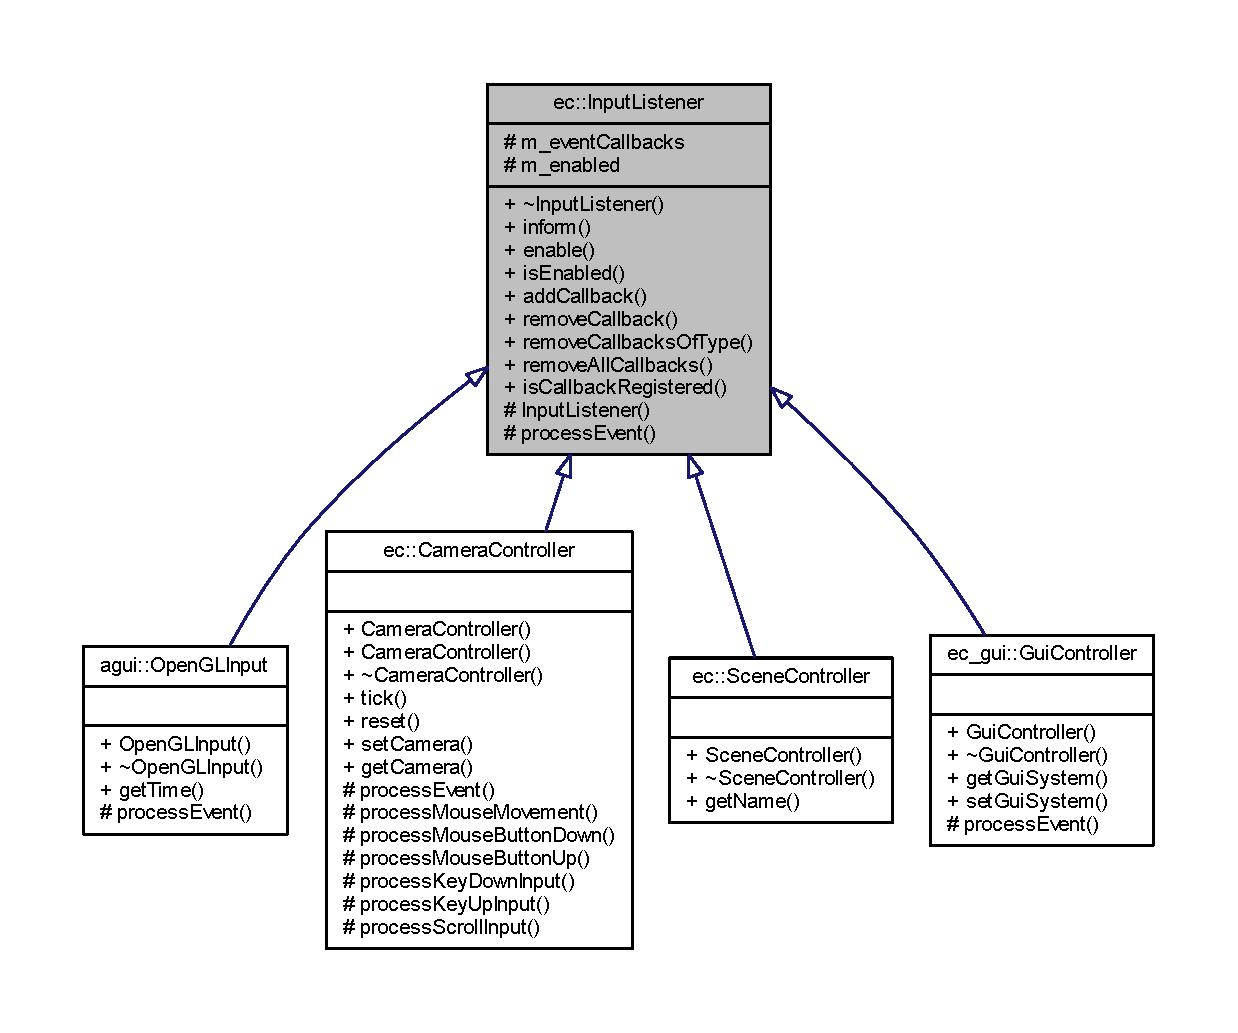
\includegraphics[width=350pt]{classec_1_1_input_listener__inherit__graph}
\end{center}
\end{figure}


Collaboration diagram for ec\+:\+:Input\+Listener\+:\nopagebreak
\begin{figure}[H]
\begin{center}
\leavevmode
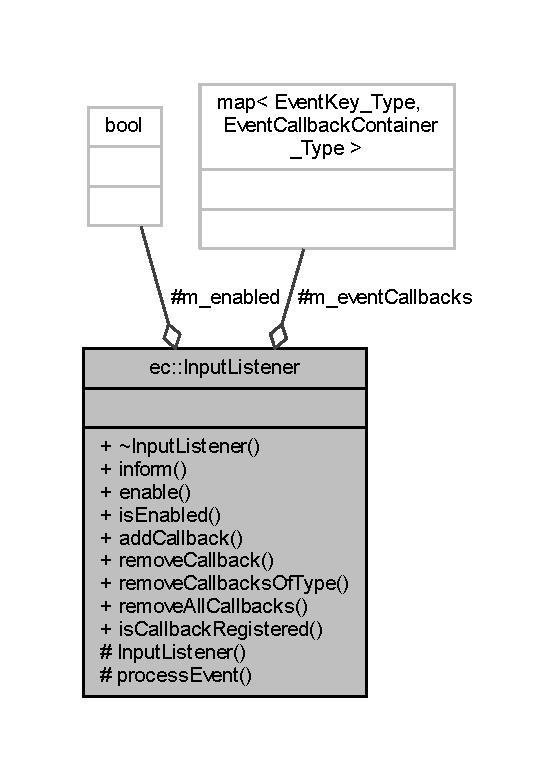
\includegraphics[width=322pt]{classec_1_1_input_listener__coll__graph}
\end{center}
\end{figure}
\subsection*{Public Types}
\begin{DoxyCompactItemize}
\item 
using \mbox{\hyperlink{classec_1_1_input_listener_af5dfb691564fa8e05fcf7f053e3c532b}{Event\+Key\+\_\+\+Type}} = \mbox{\hyperlink{namespaceec_ae2d697393ea83b34b18ab14eb5dacbca}{Input\+Type}}
\item 
using \mbox{\hyperlink{classec_1_1_input_listener_aa622615b11dfc5cd1dce423fafe27c93}{Event\+Callback\+\_\+\+Type}} = std\+::function$<$ void(const \mbox{\hyperlink{structec_1_1_input_event}{Input\+Event}} \&event)$>$
\item 
using \mbox{\hyperlink{classec_1_1_input_listener_a0d9334fafd46399a39448fe00fad3c2e}{Event\+Callback\+Container\+\_\+\+Type}} = std\+::vector$<$ \mbox{\hyperlink{classec_1_1_input_listener_aa622615b11dfc5cd1dce423fafe27c93}{Event\+Callback\+\_\+\+Type}} $>$
\item 
using \mbox{\hyperlink{classec_1_1_input_listener_abf0825f1f31a1373c5c03e51da123148}{Callback\+Container\+Map\+\_\+\+Type}} = std\+::array$<$ \mbox{\hyperlink{classec_1_1_input_listener_a0d9334fafd46399a39448fe00fad3c2e}{Event\+Callback\+Container\+\_\+\+Type}}, static\+\_\+cast$<$ int $>$(\mbox{\hyperlink{namespaceec_a30e2a743ebdeb02ac68a6cfa50f629c7ae2942a04780e223b215eb8b663cf5353}{Input\+Type\+::count}})$>$
\end{DoxyCompactItemize}
\subsection*{Public Member Functions}
\begin{DoxyCompactItemize}
\item 
virtual \mbox{\hyperlink{classec_1_1_input_listener_afd65ca201e735f5758646d6653f42804}{$\sim$\+Input\+Listener}} ()
\item 
void \mbox{\hyperlink{classec_1_1_input_listener_a39e0803651e945e177336df2cf84d61b}{inform}} (const \mbox{\hyperlink{structec_1_1_input_event}{Input\+Event}} \&event)
\begin{DoxyCompactList}\small\item\em Inform this controller about an event. \end{DoxyCompactList}\item 
virtual void \mbox{\hyperlink{classec_1_1_input_listener_a459a44443e7de70e854c2175b6c6914d}{enable}} (bool enabled)
\begin{DoxyCompactList}\small\item\em Enable or disable the evaluation of input. \end{DoxyCompactList}\item 
virtual bool \mbox{\hyperlink{classec_1_1_input_listener_a6d7a4e04543e3a86745261d9fefcbfc1}{is\+Enabled}} () const
\begin{DoxyCompactList}\small\item\em Check if this input listener is processing events. \end{DoxyCompactList}\item 
void \mbox{\hyperlink{classec_1_1_input_listener_a803faa5cc3d7576a603944cc378a7246}{add\+Callback}} (\mbox{\hyperlink{classec_1_1_input_listener_af5dfb691564fa8e05fcf7f053e3c532b}{Event\+Key\+\_\+\+Type}} key, \mbox{\hyperlink{classec_1_1_input_listener_aa622615b11dfc5cd1dce423fafe27c93}{Event\+Callback\+\_\+\+Type}} callback)
\item 
void \mbox{\hyperlink{classec_1_1_input_listener_a66e75fbfd13ec7cf87be9bebf2e02be8}{remove\+Callbacks\+Of\+Type}} (\mbox{\hyperlink{classec_1_1_input_listener_af5dfb691564fa8e05fcf7f053e3c532b}{Event\+Key\+\_\+\+Type}} key)
\begin{DoxyCompactList}\small\item\em Remove one specific or multiple callbacks. \end{DoxyCompactList}\item 
void \mbox{\hyperlink{classec_1_1_input_listener_ab3c4085477da60677e0a0659f750ead4}{remove\+All\+Callbacks}} ()
\begin{DoxyCompactList}\small\item\em Remove all registered callbacks. \end{DoxyCompactList}\end{DoxyCompactItemize}
\subsection*{Protected Member Functions}
\begin{DoxyCompactItemize}
\item 
\mbox{\hyperlink{classec_1_1_input_listener_aa44d25c2b2d3ef5e72611831fd66e10c}{Input\+Listener}} ()
\item 
virtual void \mbox{\hyperlink{classec_1_1_input_listener_a9ceaefc79c6b0b260e88454616137840}{process\+Event}} (const \mbox{\hyperlink{structec_1_1_input_event}{Input\+Event}} \&event)
\begin{DoxyCompactList}\small\item\em Automatically called, when informed about an event. \end{DoxyCompactList}\end{DoxyCompactItemize}
\subsection*{Protected Attributes}
\begin{DoxyCompactItemize}
\item 
\mbox{\hyperlink{classec_1_1_input_listener_abf0825f1f31a1373c5c03e51da123148}{Callback\+Container\+Map\+\_\+\+Type}} \mbox{\hyperlink{classec_1_1_input_listener_a4553825c97688ab1827d6f4849c92b61}{m\+\_\+callback\+Containers}}
\item 
bool \mbox{\hyperlink{classec_1_1_input_listener_af36b5fc46ed59886d73b1613aaef5a47}{m\+\_\+enabled}}
\end{DoxyCompactItemize}


\subsection{Detailed Description}
An \mbox{\hyperlink{classec_1_1_input_listener}{Input\+Listener}} can react on incoming events. It can either be used as a base class or be filled with callbacks. 

\subsection{Member Typedef Documentation}
\mbox{\Hypertarget{classec_1_1_input_listener_abf0825f1f31a1373c5c03e51da123148}\label{classec_1_1_input_listener_abf0825f1f31a1373c5c03e51da123148}} 
\index{ec\+::\+Input\+Listener@{ec\+::\+Input\+Listener}!Callback\+Container\+Map\+\_\+\+Type@{Callback\+Container\+Map\+\_\+\+Type}}
\index{Callback\+Container\+Map\+\_\+\+Type@{Callback\+Container\+Map\+\_\+\+Type}!ec\+::\+Input\+Listener@{ec\+::\+Input\+Listener}}
\subsubsection{\texorpdfstring{Callback\+Container\+Map\+\_\+\+Type}{CallbackContainerMap\_Type}}
{\footnotesize\ttfamily using \mbox{\hyperlink{classec_1_1_input_listener_abf0825f1f31a1373c5c03e51da123148}{ec\+::\+Input\+Listener\+::\+Callback\+Container\+Map\+\_\+\+Type}} =  std\+::array$<$\mbox{\hyperlink{classec_1_1_input_listener_a0d9334fafd46399a39448fe00fad3c2e}{Event\+Callback\+Container\+\_\+\+Type}}, static\+\_\+cast$<$int$>$(\mbox{\hyperlink{namespaceec_a30e2a743ebdeb02ac68a6cfa50f629c7ae2942a04780e223b215eb8b663cf5353}{Input\+Type\+::count}})$>$}

\mbox{\Hypertarget{classec_1_1_input_listener_aa622615b11dfc5cd1dce423fafe27c93}\label{classec_1_1_input_listener_aa622615b11dfc5cd1dce423fafe27c93}} 
\index{ec\+::\+Input\+Listener@{ec\+::\+Input\+Listener}!Event\+Callback\+\_\+\+Type@{Event\+Callback\+\_\+\+Type}}
\index{Event\+Callback\+\_\+\+Type@{Event\+Callback\+\_\+\+Type}!ec\+::\+Input\+Listener@{ec\+::\+Input\+Listener}}
\subsubsection{\texorpdfstring{Event\+Callback\+\_\+\+Type}{EventCallback\_Type}}
{\footnotesize\ttfamily using \mbox{\hyperlink{classec_1_1_input_listener_aa622615b11dfc5cd1dce423fafe27c93}{ec\+::\+Input\+Listener\+::\+Event\+Callback\+\_\+\+Type}} =  std\+::function$<$void(const \mbox{\hyperlink{structec_1_1_input_event}{Input\+Event}}\& event)$>$}

\mbox{\Hypertarget{classec_1_1_input_listener_a0d9334fafd46399a39448fe00fad3c2e}\label{classec_1_1_input_listener_a0d9334fafd46399a39448fe00fad3c2e}} 
\index{ec\+::\+Input\+Listener@{ec\+::\+Input\+Listener}!Event\+Callback\+Container\+\_\+\+Type@{Event\+Callback\+Container\+\_\+\+Type}}
\index{Event\+Callback\+Container\+\_\+\+Type@{Event\+Callback\+Container\+\_\+\+Type}!ec\+::\+Input\+Listener@{ec\+::\+Input\+Listener}}
\subsubsection{\texorpdfstring{Event\+Callback\+Container\+\_\+\+Type}{EventCallbackContainer\_Type}}
{\footnotesize\ttfamily using \mbox{\hyperlink{classec_1_1_input_listener_a0d9334fafd46399a39448fe00fad3c2e}{ec\+::\+Input\+Listener\+::\+Event\+Callback\+Container\+\_\+\+Type}} =  std\+::vector$<$\mbox{\hyperlink{classec_1_1_input_listener_aa622615b11dfc5cd1dce423fafe27c93}{Event\+Callback\+\_\+\+Type}}$>$}

\mbox{\Hypertarget{classec_1_1_input_listener_af5dfb691564fa8e05fcf7f053e3c532b}\label{classec_1_1_input_listener_af5dfb691564fa8e05fcf7f053e3c532b}} 
\index{ec\+::\+Input\+Listener@{ec\+::\+Input\+Listener}!Event\+Key\+\_\+\+Type@{Event\+Key\+\_\+\+Type}}
\index{Event\+Key\+\_\+\+Type@{Event\+Key\+\_\+\+Type}!ec\+::\+Input\+Listener@{ec\+::\+Input\+Listener}}
\subsubsection{\texorpdfstring{Event\+Key\+\_\+\+Type}{EventKey\_Type}}
{\footnotesize\ttfamily using \mbox{\hyperlink{classec_1_1_input_listener_af5dfb691564fa8e05fcf7f053e3c532b}{ec\+::\+Input\+Listener\+::\+Event\+Key\+\_\+\+Type}} =  \mbox{\hyperlink{namespaceec_ae2d697393ea83b34b18ab14eb5dacbca}{Input\+Type}}}



\subsection{Constructor \& Destructor Documentation}
\mbox{\Hypertarget{classec_1_1_input_listener_afd65ca201e735f5758646d6653f42804}\label{classec_1_1_input_listener_afd65ca201e735f5758646d6653f42804}} 
\index{ec\+::\+Input\+Listener@{ec\+::\+Input\+Listener}!````~Input\+Listener@{$\sim$\+Input\+Listener}}
\index{````~Input\+Listener@{$\sim$\+Input\+Listener}!ec\+::\+Input\+Listener@{ec\+::\+Input\+Listener}}
\subsubsection{\texorpdfstring{$\sim$\+Input\+Listener()}{~InputListener()}}
{\footnotesize\ttfamily ec\+::\+Input\+Listener\+::$\sim$\+Input\+Listener (\begin{DoxyParamCaption}{ }\end{DoxyParamCaption})\hspace{0.3cm}{\ttfamily [virtual]}, {\ttfamily [default]}}

\mbox{\Hypertarget{classec_1_1_input_listener_aa44d25c2b2d3ef5e72611831fd66e10c}\label{classec_1_1_input_listener_aa44d25c2b2d3ef5e72611831fd66e10c}} 
\index{ec\+::\+Input\+Listener@{ec\+::\+Input\+Listener}!Input\+Listener@{Input\+Listener}}
\index{Input\+Listener@{Input\+Listener}!ec\+::\+Input\+Listener@{ec\+::\+Input\+Listener}}
\subsubsection{\texorpdfstring{Input\+Listener()}{InputListener()}}
{\footnotesize\ttfamily ec\+::\+Input\+Listener\+::\+Input\+Listener (\begin{DoxyParamCaption}{ }\end{DoxyParamCaption})\hspace{0.3cm}{\ttfamily [explicit]}, {\ttfamily [protected]}}



\subsection{Member Function Documentation}
\mbox{\Hypertarget{classec_1_1_input_listener_a803faa5cc3d7576a603944cc378a7246}\label{classec_1_1_input_listener_a803faa5cc3d7576a603944cc378a7246}} 
\index{ec\+::\+Input\+Listener@{ec\+::\+Input\+Listener}!add\+Callback@{add\+Callback}}
\index{add\+Callback@{add\+Callback}!ec\+::\+Input\+Listener@{ec\+::\+Input\+Listener}}
\subsubsection{\texorpdfstring{add\+Callback()}{addCallback()}}
{\footnotesize\ttfamily void ec\+::\+Input\+Listener\+::add\+Callback (\begin{DoxyParamCaption}\item[{\mbox{\hyperlink{classec_1_1_input_listener_af5dfb691564fa8e05fcf7f053e3c532b}{Event\+Key\+\_\+\+Type}}}]{key,  }\item[{\mbox{\hyperlink{classec_1_1_input_listener_aa622615b11dfc5cd1dce423fafe27c93}{Event\+Callback\+\_\+\+Type}}}]{callback }\end{DoxyParamCaption})}

\mbox{\Hypertarget{classec_1_1_input_listener_a459a44443e7de70e854c2175b6c6914d}\label{classec_1_1_input_listener_a459a44443e7de70e854c2175b6c6914d}} 
\index{ec\+::\+Input\+Listener@{ec\+::\+Input\+Listener}!enable@{enable}}
\index{enable@{enable}!ec\+::\+Input\+Listener@{ec\+::\+Input\+Listener}}
\subsubsection{\texorpdfstring{enable()}{enable()}}
{\footnotesize\ttfamily void ec\+::\+Input\+Listener\+::enable (\begin{DoxyParamCaption}\item[{bool}]{enabled }\end{DoxyParamCaption})\hspace{0.3cm}{\ttfamily [virtual]}}



Enable or disable the evaluation of input. 


\begin{DoxyParams}{Parameters}
{\em enabled} & If true incoming events will be processed. \\
\hline
\end{DoxyParams}
\mbox{\Hypertarget{classec_1_1_input_listener_a39e0803651e945e177336df2cf84d61b}\label{classec_1_1_input_listener_a39e0803651e945e177336df2cf84d61b}} 
\index{ec\+::\+Input\+Listener@{ec\+::\+Input\+Listener}!inform@{inform}}
\index{inform@{inform}!ec\+::\+Input\+Listener@{ec\+::\+Input\+Listener}}
\subsubsection{\texorpdfstring{inform()}{inform()}}
{\footnotesize\ttfamily void ec\+::\+Input\+Listener\+::inform (\begin{DoxyParamCaption}\item[{const \mbox{\hyperlink{structec_1_1_input_event}{Input\+Event}} \&}]{event }\end{DoxyParamCaption})}



Inform this controller about an event. 


\begin{DoxyParams}{Parameters}
{\em event} & The event to process. \\
\hline
\end{DoxyParams}
\mbox{\Hypertarget{classec_1_1_input_listener_a6d7a4e04543e3a86745261d9fefcbfc1}\label{classec_1_1_input_listener_a6d7a4e04543e3a86745261d9fefcbfc1}} 
\index{ec\+::\+Input\+Listener@{ec\+::\+Input\+Listener}!is\+Enabled@{is\+Enabled}}
\index{is\+Enabled@{is\+Enabled}!ec\+::\+Input\+Listener@{ec\+::\+Input\+Listener}}
\subsubsection{\texorpdfstring{is\+Enabled()}{isEnabled()}}
{\footnotesize\ttfamily bool ec\+::\+Input\+Listener\+::is\+Enabled (\begin{DoxyParamCaption}{ }\end{DoxyParamCaption}) const\hspace{0.3cm}{\ttfamily [virtual]}}



Check if this input listener is processing events. 

\mbox{\Hypertarget{classec_1_1_input_listener_a9ceaefc79c6b0b260e88454616137840}\label{classec_1_1_input_listener_a9ceaefc79c6b0b260e88454616137840}} 
\index{ec\+::\+Input\+Listener@{ec\+::\+Input\+Listener}!process\+Event@{process\+Event}}
\index{process\+Event@{process\+Event}!ec\+::\+Input\+Listener@{ec\+::\+Input\+Listener}}
\subsubsection{\texorpdfstring{process\+Event()}{processEvent()}}
{\footnotesize\ttfamily void ec\+::\+Input\+Listener\+::process\+Event (\begin{DoxyParamCaption}\item[{const \mbox{\hyperlink{structec_1_1_input_event}{Input\+Event}} \&}]{event }\end{DoxyParamCaption})\hspace{0.3cm}{\ttfamily [protected]}, {\ttfamily [virtual]}}



Automatically called, when informed about an event. 



Reimplemented in \mbox{\hyperlink{classec_1_1_camera_controller_af44aad5f80005eaadf5d637b3b00c6d6}{ec\+::\+Camera\+Controller}}, and \mbox{\hyperlink{classec_1_1_open_g_l_input_a064a4e318e18d79ad8df19c789f84686}{ec\+::\+Open\+G\+L\+Input}}.

\mbox{\Hypertarget{classec_1_1_input_listener_ab3c4085477da60677e0a0659f750ead4}\label{classec_1_1_input_listener_ab3c4085477da60677e0a0659f750ead4}} 
\index{ec\+::\+Input\+Listener@{ec\+::\+Input\+Listener}!remove\+All\+Callbacks@{remove\+All\+Callbacks}}
\index{remove\+All\+Callbacks@{remove\+All\+Callbacks}!ec\+::\+Input\+Listener@{ec\+::\+Input\+Listener}}
\subsubsection{\texorpdfstring{remove\+All\+Callbacks()}{removeAllCallbacks()}}
{\footnotesize\ttfamily void ec\+::\+Input\+Listener\+::remove\+All\+Callbacks (\begin{DoxyParamCaption}{ }\end{DoxyParamCaption})}



Remove all registered callbacks. 

\mbox{\Hypertarget{classec_1_1_input_listener_a66e75fbfd13ec7cf87be9bebf2e02be8}\label{classec_1_1_input_listener_a66e75fbfd13ec7cf87be9bebf2e02be8}} 
\index{ec\+::\+Input\+Listener@{ec\+::\+Input\+Listener}!remove\+Callbacks\+Of\+Type@{remove\+Callbacks\+Of\+Type}}
\index{remove\+Callbacks\+Of\+Type@{remove\+Callbacks\+Of\+Type}!ec\+::\+Input\+Listener@{ec\+::\+Input\+Listener}}
\subsubsection{\texorpdfstring{remove\+Callbacks\+Of\+Type()}{removeCallbacksOfType()}}
{\footnotesize\ttfamily void ec\+::\+Input\+Listener\+::remove\+Callbacks\+Of\+Type (\begin{DoxyParamCaption}\item[{\mbox{\hyperlink{classec_1_1_input_listener_af5dfb691564fa8e05fcf7f053e3c532b}{Event\+Key\+\_\+\+Type}}}]{key }\end{DoxyParamCaption})}



Remove one specific or multiple callbacks. 


\begin{DoxyParams}{Parameters}
{\em key} & The type of the callbacks to remove. \\
\hline
\end{DoxyParams}


\subsection{Member Data Documentation}
\mbox{\Hypertarget{classec_1_1_input_listener_a4553825c97688ab1827d6f4849c92b61}\label{classec_1_1_input_listener_a4553825c97688ab1827d6f4849c92b61}} 
\index{ec\+::\+Input\+Listener@{ec\+::\+Input\+Listener}!m\+\_\+callback\+Containers@{m\+\_\+callback\+Containers}}
\index{m\+\_\+callback\+Containers@{m\+\_\+callback\+Containers}!ec\+::\+Input\+Listener@{ec\+::\+Input\+Listener}}
\subsubsection{\texorpdfstring{m\+\_\+callback\+Containers}{m\_callbackContainers}}
{\footnotesize\ttfamily \mbox{\hyperlink{classec_1_1_input_listener_abf0825f1f31a1373c5c03e51da123148}{Callback\+Container\+Map\+\_\+\+Type}} ec\+::\+Input\+Listener\+::m\+\_\+callback\+Containers\hspace{0.3cm}{\ttfamily [protected]}}

\mbox{\Hypertarget{classec_1_1_input_listener_af36b5fc46ed59886d73b1613aaef5a47}\label{classec_1_1_input_listener_af36b5fc46ed59886d73b1613aaef5a47}} 
\index{ec\+::\+Input\+Listener@{ec\+::\+Input\+Listener}!m\+\_\+enabled@{m\+\_\+enabled}}
\index{m\+\_\+enabled@{m\+\_\+enabled}!ec\+::\+Input\+Listener@{ec\+::\+Input\+Listener}}
\subsubsection{\texorpdfstring{m\+\_\+enabled}{m\_enabled}}
{\footnotesize\ttfamily bool ec\+::\+Input\+Listener\+::m\+\_\+enabled\hspace{0.3cm}{\ttfamily [protected]}}



The documentation for this class was generated from the following files\+:\begin{DoxyCompactItemize}
\item 
D\+:/\+Library/\+Documents/\+Job/\+Forschungsmaster/\+Projekte/\+Simulation\+Visualization/\+Eye\+Candy3\+D/\+Eye\+Candy3\+D/include/\+E\+C3\+D/\+Core/\mbox{\hyperlink{_input_listener_8h}{Input\+Listener.\+h}}\item 
D\+:/\+Library/\+Documents/\+Job/\+Forschungsmaster/\+Projekte/\+Simulation\+Visualization/\+Eye\+Candy3\+D/\+Eye\+Candy3\+D/src/\+Core/\mbox{\hyperlink{_input_listener_8cpp}{Input\+Listener.\+cpp}}\end{DoxyCompactItemize}

\hypertarget{classec_1_1_input_observable}{}\section{ec\+:\+:Input\+Observable Class Reference}
\label{classec_1_1_input_observable}\index{ec\+::\+Input\+Observable@{ec\+::\+Input\+Observable}}


{\ttfamily \#include $<$Input\+Observable.\+h$>$}



Collaboration diagram for ec\+:\+:Input\+Observable\+:\nopagebreak
\begin{figure}[H]
\begin{center}
\leavevmode
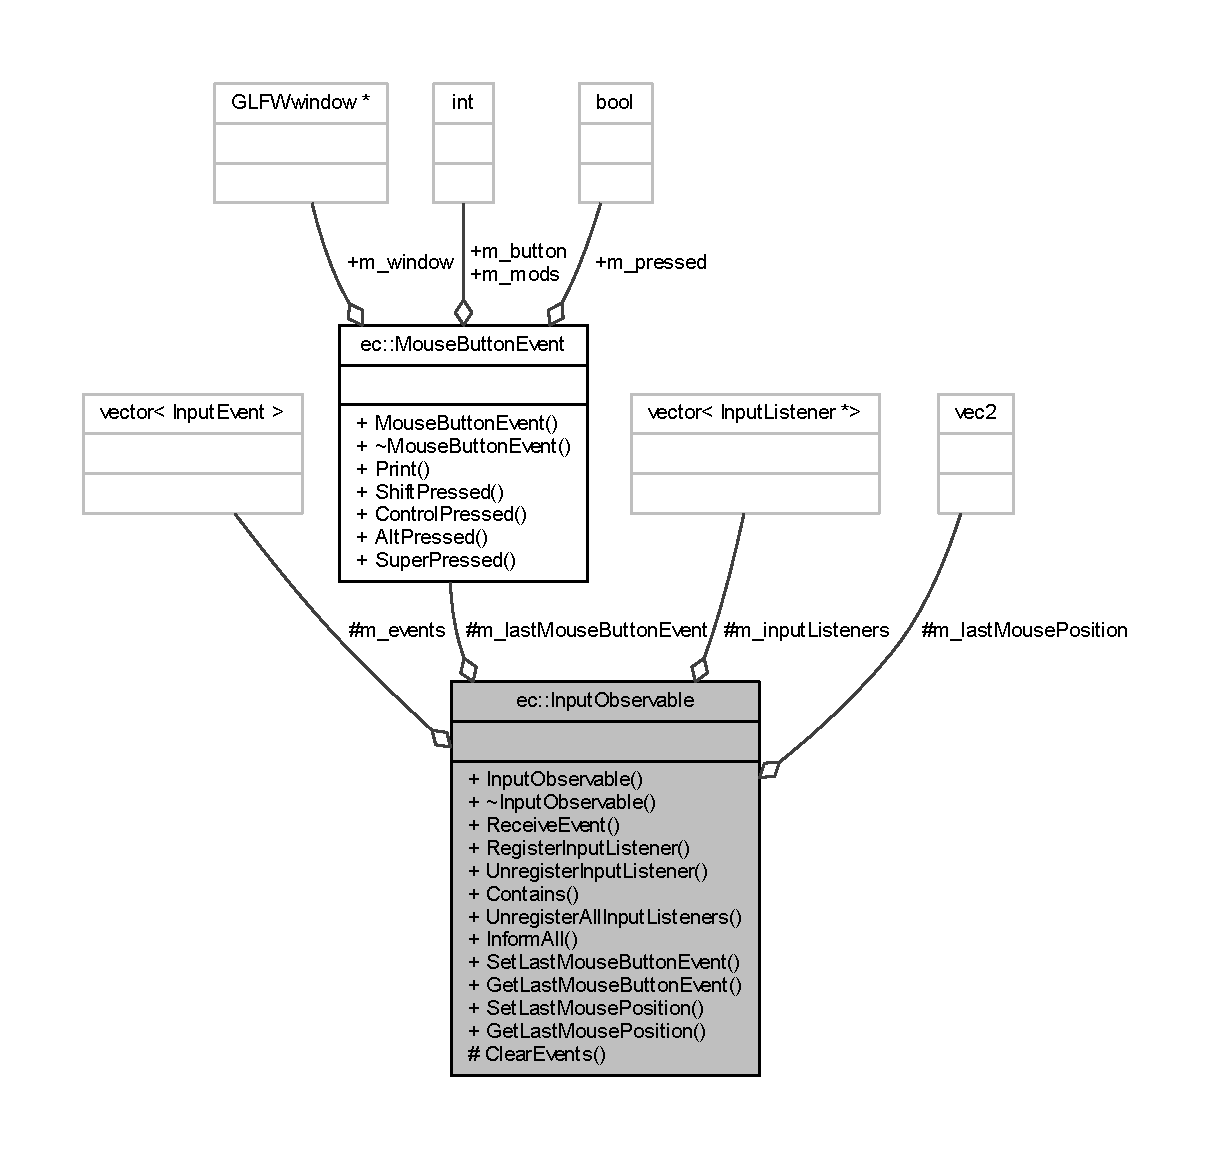
\includegraphics[width=350pt]{classec_1_1_input_observable__coll__graph}
\end{center}
\end{figure}
\subsection*{Public Types}
\begin{DoxyCompactItemize}
\item 
using \mbox{\hyperlink{classec_1_1_input_observable_a99717b2918621597db89d9ede34ddded}{Input\+Listeners\+\_\+T}} = std\+::vector$<$ \mbox{\hyperlink{classec_1_1_input_listener}{Input\+Listener}} $\ast$ $>$
\item 
using \mbox{\hyperlink{classec_1_1_input_observable_a9b63c8acbcbfc0f99d2964493ac52925}{Events\+\_\+T}} = std\+::vector$<$ \mbox{\hyperlink{structec_1_1_input_event}{Input\+Event}} $>$
\end{DoxyCompactItemize}
\subsection*{Public Member Functions}
\begin{DoxyCompactItemize}
\item 
\mbox{\hyperlink{classec_1_1_input_observable_a92422814189d1210f631f4d1378877f3}{Input\+Observable}} ()
\item 
virtual \mbox{\hyperlink{classec_1_1_input_observable_ac261f6a73cfdcd37c276e732cc25f869}{$\sim$\+Input\+Observable}} ()
\item 
virtual void \mbox{\hyperlink{classec_1_1_input_observable_ac35d29f643a2735e4cb38cb6ee1354aa}{receive\+Event}} (const \mbox{\hyperlink{structec_1_1_input_event}{Input\+Event}} \&event)
\item 
virtual void \mbox{\hyperlink{classec_1_1_input_observable_a542bd14ecfbeceed917ea0df5c7f3755}{register\+Input\+Listener}} (\mbox{\hyperlink{classec_1_1_input_listener}{Input\+Listener}} $\ast$input\+Listener)
\item 
virtual bool \mbox{\hyperlink{classec_1_1_input_observable_aab1af4952f6127781eade6dccf33aafb}{unregister\+Input\+Listener}} (\mbox{\hyperlink{classec_1_1_input_listener}{Input\+Listener}} $\ast$input\+Listener)
\item 
virtual bool \mbox{\hyperlink{classec_1_1_input_observable_a6e14f68359b8d7e1be60e8503a07ea87}{contains}} (\mbox{\hyperlink{classec_1_1_input_listener}{Input\+Listener}} $\ast$input\+Listener)
\item 
virtual void \mbox{\hyperlink{classec_1_1_input_observable_ac8d3ed43a3b26601e2710e3758248620}{unregister\+All\+Input\+Listeners}} ()
\item 
virtual void \mbox{\hyperlink{classec_1_1_input_observable_ac8ac61eaebb95010e8a12bb1e6348391}{inform\+All}} ()
\item 
void \mbox{\hyperlink{classec_1_1_input_observable_abcd9d6067210ea7751824b619147a65c}{set\+Last\+Prev\+Mouse\+Event}} (const \mbox{\hyperlink{structec_1_1_mouse_event}{Mouse\+Event}} \&event)
\item 
const \mbox{\hyperlink{structec_1_1_mouse_event}{Mouse\+Event}} \& \mbox{\hyperlink{classec_1_1_input_observable_abf9f1388171a99581a0a4100bbf2d11b}{get\+Prev\+Mouse\+Event}} () const
\item 
void \mbox{\hyperlink{classec_1_1_input_observable_afcc8abf8d747417f50465189e632d0dd}{set\+Prev\+Keyboard\+Event}} (const \mbox{\hyperlink{structec_1_1_keyboard_event}{Keyboard\+Event}} \&event)
\item 
const \mbox{\hyperlink{structec_1_1_keyboard_event}{Keyboard\+Event}} \& \mbox{\hyperlink{classec_1_1_input_observable_ab1ba2fa8deaf1d69a4809e4d8dc61452}{get\+Prev\+Keyboard\+Event}} () const
\item 
void \mbox{\hyperlink{classec_1_1_input_observable_a55c7310a50dc873f69c2246bbeeed3e6}{set\+Prev\+Display\+Event}} (const \mbox{\hyperlink{structec_1_1_display_event}{Display\+Event}} \&event)
\item 
const \mbox{\hyperlink{structec_1_1_display_event}{Display\+Event}} \& \mbox{\hyperlink{classec_1_1_input_observable_ac12e711d3a7dcaf65d2028d2283c1243}{get\+Prev\+Display\+Event}} () const
\end{DoxyCompactItemize}
\subsection*{Protected Member Functions}
\begin{DoxyCompactItemize}
\item 
\mbox{\hyperlink{structec_1_1_input_event}{Input\+Event}} \mbox{\hyperlink{classec_1_1_input_observable_a7aaa88f25dd3d8902bc6767240c83ecf}{prepare\+Event}} (const \mbox{\hyperlink{structec_1_1_input_event}{Input\+Event}} \&event)
\item 
virtual void \mbox{\hyperlink{classec_1_1_input_observable_a799c88abda6814473fe486654205f07b}{clear\+Events}} ()
\end{DoxyCompactItemize}
\subsection*{Protected Attributes}
\begin{DoxyCompactItemize}
\item 
\mbox{\hyperlink{classec_1_1_input_observable_a99717b2918621597db89d9ede34ddded}{Input\+Listeners\+\_\+T}} \mbox{\hyperlink{classec_1_1_input_observable_aa11756df5cac4e93ace9db3f6c8817c4}{m\+\_\+input\+Listeners}}
\item 
\mbox{\hyperlink{classec_1_1_input_observable_a9b63c8acbcbfc0f99d2964493ac52925}{Events\+\_\+T}} \mbox{\hyperlink{classec_1_1_input_observable_af83e9f99bec60cdce82b129fa457c6ab}{m\+\_\+events}}
\item 
\mbox{\hyperlink{structec_1_1_mouse_event}{Mouse\+Event}} \mbox{\hyperlink{classec_1_1_input_observable_a99e8c1484fe87503096e681d8bd3b75f}{m\+\_\+prev\+Mouse\+Event}}
\item 
\mbox{\hyperlink{structec_1_1_keyboard_event}{Keyboard\+Event}} \mbox{\hyperlink{classec_1_1_input_observable_acf14cdeb5a394fbd296ff3dfb391c14f}{m\+\_\+prev\+Keyboard\+Event}}
\item 
\mbox{\hyperlink{structec_1_1_display_event}{Display\+Event}} \mbox{\hyperlink{classec_1_1_input_observable_ae480593ec25d98ea00b0b7a9aa6cba32}{m\+\_\+prev\+Display\+Event}}
\end{DoxyCompactItemize}


\subsection{Member Typedef Documentation}
\mbox{\Hypertarget{classec_1_1_input_observable_a9b63c8acbcbfc0f99d2964493ac52925}\label{classec_1_1_input_observable_a9b63c8acbcbfc0f99d2964493ac52925}} 
\index{ec\+::\+Input\+Observable@{ec\+::\+Input\+Observable}!Events\+\_\+T@{Events\+\_\+T}}
\index{Events\+\_\+T@{Events\+\_\+T}!ec\+::\+Input\+Observable@{ec\+::\+Input\+Observable}}
\subsubsection{\texorpdfstring{Events\+\_\+T}{Events\_T}}
{\footnotesize\ttfamily using \mbox{\hyperlink{classec_1_1_input_observable_a9b63c8acbcbfc0f99d2964493ac52925}{ec\+::\+Input\+Observable\+::\+Events\+\_\+T}} =  std\+::vector$<$\mbox{\hyperlink{structec_1_1_input_event}{Input\+Event}}$>$}

\mbox{\Hypertarget{classec_1_1_input_observable_a99717b2918621597db89d9ede34ddded}\label{classec_1_1_input_observable_a99717b2918621597db89d9ede34ddded}} 
\index{ec\+::\+Input\+Observable@{ec\+::\+Input\+Observable}!Input\+Listeners\+\_\+T@{Input\+Listeners\+\_\+T}}
\index{Input\+Listeners\+\_\+T@{Input\+Listeners\+\_\+T}!ec\+::\+Input\+Observable@{ec\+::\+Input\+Observable}}
\subsubsection{\texorpdfstring{Input\+Listeners\+\_\+T}{InputListeners\_T}}
{\footnotesize\ttfamily using \mbox{\hyperlink{classec_1_1_input_observable_a99717b2918621597db89d9ede34ddded}{ec\+::\+Input\+Observable\+::\+Input\+Listeners\+\_\+T}} =  std\+::vector$<$\mbox{\hyperlink{classec_1_1_input_listener}{Input\+Listener}}$\ast$$>$}



\subsection{Constructor \& Destructor Documentation}
\mbox{\Hypertarget{classec_1_1_input_observable_a92422814189d1210f631f4d1378877f3}\label{classec_1_1_input_observable_a92422814189d1210f631f4d1378877f3}} 
\index{ec\+::\+Input\+Observable@{ec\+::\+Input\+Observable}!Input\+Observable@{Input\+Observable}}
\index{Input\+Observable@{Input\+Observable}!ec\+::\+Input\+Observable@{ec\+::\+Input\+Observable}}
\subsubsection{\texorpdfstring{Input\+Observable()}{InputObservable()}}
{\footnotesize\ttfamily ec\+::\+Input\+Observable\+::\+Input\+Observable (\begin{DoxyParamCaption}{ }\end{DoxyParamCaption})\hspace{0.3cm}{\ttfamily [explicit]}, {\ttfamily [default]}}

\mbox{\Hypertarget{classec_1_1_input_observable_ac261f6a73cfdcd37c276e732cc25f869}\label{classec_1_1_input_observable_ac261f6a73cfdcd37c276e732cc25f869}} 
\index{ec\+::\+Input\+Observable@{ec\+::\+Input\+Observable}!````~Input\+Observable@{$\sim$\+Input\+Observable}}
\index{````~Input\+Observable@{$\sim$\+Input\+Observable}!ec\+::\+Input\+Observable@{ec\+::\+Input\+Observable}}
\subsubsection{\texorpdfstring{$\sim$\+Input\+Observable()}{~InputObservable()}}
{\footnotesize\ttfamily ec\+::\+Input\+Observable\+::$\sim$\+Input\+Observable (\begin{DoxyParamCaption}{ }\end{DoxyParamCaption})\hspace{0.3cm}{\ttfamily [virtual]}, {\ttfamily [default]}}



\subsection{Member Function Documentation}
\mbox{\Hypertarget{classec_1_1_input_observable_a799c88abda6814473fe486654205f07b}\label{classec_1_1_input_observable_a799c88abda6814473fe486654205f07b}} 
\index{ec\+::\+Input\+Observable@{ec\+::\+Input\+Observable}!clear\+Events@{clear\+Events}}
\index{clear\+Events@{clear\+Events}!ec\+::\+Input\+Observable@{ec\+::\+Input\+Observable}}
\subsubsection{\texorpdfstring{clear\+Events()}{clearEvents()}}
{\footnotesize\ttfamily void ec\+::\+Input\+Observable\+::clear\+Events (\begin{DoxyParamCaption}{ }\end{DoxyParamCaption})\hspace{0.3cm}{\ttfamily [protected]}, {\ttfamily [virtual]}}

\mbox{\Hypertarget{classec_1_1_input_observable_a6e14f68359b8d7e1be60e8503a07ea87}\label{classec_1_1_input_observable_a6e14f68359b8d7e1be60e8503a07ea87}} 
\index{ec\+::\+Input\+Observable@{ec\+::\+Input\+Observable}!contains@{contains}}
\index{contains@{contains}!ec\+::\+Input\+Observable@{ec\+::\+Input\+Observable}}
\subsubsection{\texorpdfstring{contains()}{contains()}}
{\footnotesize\ttfamily bool ec\+::\+Input\+Observable\+::contains (\begin{DoxyParamCaption}\item[{\mbox{\hyperlink{classec_1_1_input_listener}{Input\+Listener}} $\ast$}]{input\+Listener }\end{DoxyParamCaption})\hspace{0.3cm}{\ttfamily [virtual]}}

Check if this observer contains a specific controller \mbox{\Hypertarget{classec_1_1_input_observable_ac12e711d3a7dcaf65d2028d2283c1243}\label{classec_1_1_input_observable_ac12e711d3a7dcaf65d2028d2283c1243}} 
\index{ec\+::\+Input\+Observable@{ec\+::\+Input\+Observable}!get\+Prev\+Display\+Event@{get\+Prev\+Display\+Event}}
\index{get\+Prev\+Display\+Event@{get\+Prev\+Display\+Event}!ec\+::\+Input\+Observable@{ec\+::\+Input\+Observable}}
\subsubsection{\texorpdfstring{get\+Prev\+Display\+Event()}{getPrevDisplayEvent()}}
{\footnotesize\ttfamily const \mbox{\hyperlink{structec_1_1_display_event}{ec\+::\+Display\+Event}} \& ec\+::\+Input\+Observable\+::get\+Prev\+Display\+Event (\begin{DoxyParamCaption}{ }\end{DoxyParamCaption}) const}

Get the previous keyboard event \mbox{\Hypertarget{classec_1_1_input_observable_ab1ba2fa8deaf1d69a4809e4d8dc61452}\label{classec_1_1_input_observable_ab1ba2fa8deaf1d69a4809e4d8dc61452}} 
\index{ec\+::\+Input\+Observable@{ec\+::\+Input\+Observable}!get\+Prev\+Keyboard\+Event@{get\+Prev\+Keyboard\+Event}}
\index{get\+Prev\+Keyboard\+Event@{get\+Prev\+Keyboard\+Event}!ec\+::\+Input\+Observable@{ec\+::\+Input\+Observable}}
\subsubsection{\texorpdfstring{get\+Prev\+Keyboard\+Event()}{getPrevKeyboardEvent()}}
{\footnotesize\ttfamily const \mbox{\hyperlink{structec_1_1_keyboard_event}{ec\+::\+Keyboard\+Event}} \& ec\+::\+Input\+Observable\+::get\+Prev\+Keyboard\+Event (\begin{DoxyParamCaption}{ }\end{DoxyParamCaption}) const}

Get the previous keyboard event \mbox{\Hypertarget{classec_1_1_input_observable_abf9f1388171a99581a0a4100bbf2d11b}\label{classec_1_1_input_observable_abf9f1388171a99581a0a4100bbf2d11b}} 
\index{ec\+::\+Input\+Observable@{ec\+::\+Input\+Observable}!get\+Prev\+Mouse\+Event@{get\+Prev\+Mouse\+Event}}
\index{get\+Prev\+Mouse\+Event@{get\+Prev\+Mouse\+Event}!ec\+::\+Input\+Observable@{ec\+::\+Input\+Observable}}
\subsubsection{\texorpdfstring{get\+Prev\+Mouse\+Event()}{getPrevMouseEvent()}}
{\footnotesize\ttfamily const \mbox{\hyperlink{structec_1_1_mouse_event}{ec\+::\+Mouse\+Event}} \& ec\+::\+Input\+Observable\+::get\+Prev\+Mouse\+Event (\begin{DoxyParamCaption}{ }\end{DoxyParamCaption}) const}

Get the previous mouse event \mbox{\Hypertarget{classec_1_1_input_observable_ac8ac61eaebb95010e8a12bb1e6348391}\label{classec_1_1_input_observable_ac8ac61eaebb95010e8a12bb1e6348391}} 
\index{ec\+::\+Input\+Observable@{ec\+::\+Input\+Observable}!inform\+All@{inform\+All}}
\index{inform\+All@{inform\+All}!ec\+::\+Input\+Observable@{ec\+::\+Input\+Observable}}
\subsubsection{\texorpdfstring{inform\+All()}{informAll()}}
{\footnotesize\ttfamily void ec\+::\+Input\+Observable\+::inform\+All (\begin{DoxyParamCaption}{ }\end{DoxyParamCaption})\hspace{0.3cm}{\ttfamily [virtual]}}

Inform all input listeners about all accumulated events \mbox{\Hypertarget{classec_1_1_input_observable_a7aaa88f25dd3d8902bc6767240c83ecf}\label{classec_1_1_input_observable_a7aaa88f25dd3d8902bc6767240c83ecf}} 
\index{ec\+::\+Input\+Observable@{ec\+::\+Input\+Observable}!prepare\+Event@{prepare\+Event}}
\index{prepare\+Event@{prepare\+Event}!ec\+::\+Input\+Observable@{ec\+::\+Input\+Observable}}
\subsubsection{\texorpdfstring{prepare\+Event()}{prepareEvent()}}
{\footnotesize\ttfamily \mbox{\hyperlink{structec_1_1_input_event}{ec\+::\+Input\+Event}} ec\+::\+Input\+Observable\+::prepare\+Event (\begin{DoxyParamCaption}\item[{const \mbox{\hyperlink{structec_1_1_input_event}{Input\+Event}} \&}]{event }\end{DoxyParamCaption})\hspace{0.3cm}{\ttfamily [protected]}}

\mbox{\Hypertarget{classec_1_1_input_observable_ac35d29f643a2735e4cb38cb6ee1354aa}\label{classec_1_1_input_observable_ac35d29f643a2735e4cb38cb6ee1354aa}} 
\index{ec\+::\+Input\+Observable@{ec\+::\+Input\+Observable}!receive\+Event@{receive\+Event}}
\index{receive\+Event@{receive\+Event}!ec\+::\+Input\+Observable@{ec\+::\+Input\+Observable}}
\subsubsection{\texorpdfstring{receive\+Event()}{receiveEvent()}}
{\footnotesize\ttfamily void ec\+::\+Input\+Observable\+::receive\+Event (\begin{DoxyParamCaption}\item[{const \mbox{\hyperlink{structec_1_1_input_event}{Input\+Event}} \&}]{event }\end{DoxyParamCaption})\hspace{0.3cm}{\ttfamily [virtual]}}

\mbox{\Hypertarget{classec_1_1_input_observable_a542bd14ecfbeceed917ea0df5c7f3755}\label{classec_1_1_input_observable_a542bd14ecfbeceed917ea0df5c7f3755}} 
\index{ec\+::\+Input\+Observable@{ec\+::\+Input\+Observable}!register\+Input\+Listener@{register\+Input\+Listener}}
\index{register\+Input\+Listener@{register\+Input\+Listener}!ec\+::\+Input\+Observable@{ec\+::\+Input\+Observable}}
\subsubsection{\texorpdfstring{register\+Input\+Listener()}{registerInputListener()}}
{\footnotesize\ttfamily void ec\+::\+Input\+Observable\+::register\+Input\+Listener (\begin{DoxyParamCaption}\item[{\mbox{\hyperlink{classec_1_1_input_listener}{Input\+Listener}} $\ast$}]{input\+Listener }\end{DoxyParamCaption})\hspace{0.3cm}{\ttfamily [virtual]}}

Register a new or remove an old listener \mbox{\Hypertarget{classec_1_1_input_observable_abcd9d6067210ea7751824b619147a65c}\label{classec_1_1_input_observable_abcd9d6067210ea7751824b619147a65c}} 
\index{ec\+::\+Input\+Observable@{ec\+::\+Input\+Observable}!set\+Last\+Prev\+Mouse\+Event@{set\+Last\+Prev\+Mouse\+Event}}
\index{set\+Last\+Prev\+Mouse\+Event@{set\+Last\+Prev\+Mouse\+Event}!ec\+::\+Input\+Observable@{ec\+::\+Input\+Observable}}
\subsubsection{\texorpdfstring{set\+Last\+Prev\+Mouse\+Event()}{setLastPrevMouseEvent()}}
{\footnotesize\ttfamily void ec\+::\+Input\+Observable\+::set\+Last\+Prev\+Mouse\+Event (\begin{DoxyParamCaption}\item[{const \mbox{\hyperlink{structec_1_1_mouse_event}{Mouse\+Event}} \&}]{event }\end{DoxyParamCaption})}

Set the previous mouse event \mbox{\Hypertarget{classec_1_1_input_observable_a55c7310a50dc873f69c2246bbeeed3e6}\label{classec_1_1_input_observable_a55c7310a50dc873f69c2246bbeeed3e6}} 
\index{ec\+::\+Input\+Observable@{ec\+::\+Input\+Observable}!set\+Prev\+Display\+Event@{set\+Prev\+Display\+Event}}
\index{set\+Prev\+Display\+Event@{set\+Prev\+Display\+Event}!ec\+::\+Input\+Observable@{ec\+::\+Input\+Observable}}
\subsubsection{\texorpdfstring{set\+Prev\+Display\+Event()}{setPrevDisplayEvent()}}
{\footnotesize\ttfamily void ec\+::\+Input\+Observable\+::set\+Prev\+Display\+Event (\begin{DoxyParamCaption}\item[{const \mbox{\hyperlink{structec_1_1_display_event}{Display\+Event}} \&}]{event }\end{DoxyParamCaption})}

Set the previous keyboard event \mbox{\Hypertarget{classec_1_1_input_observable_afcc8abf8d747417f50465189e632d0dd}\label{classec_1_1_input_observable_afcc8abf8d747417f50465189e632d0dd}} 
\index{ec\+::\+Input\+Observable@{ec\+::\+Input\+Observable}!set\+Prev\+Keyboard\+Event@{set\+Prev\+Keyboard\+Event}}
\index{set\+Prev\+Keyboard\+Event@{set\+Prev\+Keyboard\+Event}!ec\+::\+Input\+Observable@{ec\+::\+Input\+Observable}}
\subsubsection{\texorpdfstring{set\+Prev\+Keyboard\+Event()}{setPrevKeyboardEvent()}}
{\footnotesize\ttfamily void ec\+::\+Input\+Observable\+::set\+Prev\+Keyboard\+Event (\begin{DoxyParamCaption}\item[{const \mbox{\hyperlink{structec_1_1_keyboard_event}{Keyboard\+Event}} \&}]{event }\end{DoxyParamCaption})}

Set the previous keyboard event \mbox{\Hypertarget{classec_1_1_input_observable_ac8d3ed43a3b26601e2710e3758248620}\label{classec_1_1_input_observable_ac8d3ed43a3b26601e2710e3758248620}} 
\index{ec\+::\+Input\+Observable@{ec\+::\+Input\+Observable}!unregister\+All\+Input\+Listeners@{unregister\+All\+Input\+Listeners}}
\index{unregister\+All\+Input\+Listeners@{unregister\+All\+Input\+Listeners}!ec\+::\+Input\+Observable@{ec\+::\+Input\+Observable}}
\subsubsection{\texorpdfstring{unregister\+All\+Input\+Listeners()}{unregisterAllInputListeners()}}
{\footnotesize\ttfamily void ec\+::\+Input\+Observable\+::unregister\+All\+Input\+Listeners (\begin{DoxyParamCaption}{ }\end{DoxyParamCaption})\hspace{0.3cm}{\ttfamily [virtual]}}

Clears the input listener list \mbox{\Hypertarget{classec_1_1_input_observable_aab1af4952f6127781eade6dccf33aafb}\label{classec_1_1_input_observable_aab1af4952f6127781eade6dccf33aafb}} 
\index{ec\+::\+Input\+Observable@{ec\+::\+Input\+Observable}!unregister\+Input\+Listener@{unregister\+Input\+Listener}}
\index{unregister\+Input\+Listener@{unregister\+Input\+Listener}!ec\+::\+Input\+Observable@{ec\+::\+Input\+Observable}}
\subsubsection{\texorpdfstring{unregister\+Input\+Listener()}{unregisterInputListener()}}
{\footnotesize\ttfamily bool ec\+::\+Input\+Observable\+::unregister\+Input\+Listener (\begin{DoxyParamCaption}\item[{\mbox{\hyperlink{classec_1_1_input_listener}{Input\+Listener}} $\ast$}]{input\+Listener }\end{DoxyParamCaption})\hspace{0.3cm}{\ttfamily [virtual]}}



\subsection{Member Data Documentation}
\mbox{\Hypertarget{classec_1_1_input_observable_af83e9f99bec60cdce82b129fa457c6ab}\label{classec_1_1_input_observable_af83e9f99bec60cdce82b129fa457c6ab}} 
\index{ec\+::\+Input\+Observable@{ec\+::\+Input\+Observable}!m\+\_\+events@{m\+\_\+events}}
\index{m\+\_\+events@{m\+\_\+events}!ec\+::\+Input\+Observable@{ec\+::\+Input\+Observable}}
\subsubsection{\texorpdfstring{m\+\_\+events}{m\_events}}
{\footnotesize\ttfamily \mbox{\hyperlink{classec_1_1_input_observable_a9b63c8acbcbfc0f99d2964493ac52925}{Events\+\_\+T}} ec\+::\+Input\+Observable\+::m\+\_\+events\hspace{0.3cm}{\ttfamily [protected]}}

\mbox{\Hypertarget{classec_1_1_input_observable_aa11756df5cac4e93ace9db3f6c8817c4}\label{classec_1_1_input_observable_aa11756df5cac4e93ace9db3f6c8817c4}} 
\index{ec\+::\+Input\+Observable@{ec\+::\+Input\+Observable}!m\+\_\+input\+Listeners@{m\+\_\+input\+Listeners}}
\index{m\+\_\+input\+Listeners@{m\+\_\+input\+Listeners}!ec\+::\+Input\+Observable@{ec\+::\+Input\+Observable}}
\subsubsection{\texorpdfstring{m\+\_\+input\+Listeners}{m\_inputListeners}}
{\footnotesize\ttfamily \mbox{\hyperlink{classec_1_1_input_observable_a99717b2918621597db89d9ede34ddded}{Input\+Listeners\+\_\+T}} ec\+::\+Input\+Observable\+::m\+\_\+input\+Listeners\hspace{0.3cm}{\ttfamily [protected]}}

\mbox{\Hypertarget{classec_1_1_input_observable_ae480593ec25d98ea00b0b7a9aa6cba32}\label{classec_1_1_input_observable_ae480593ec25d98ea00b0b7a9aa6cba32}} 
\index{ec\+::\+Input\+Observable@{ec\+::\+Input\+Observable}!m\+\_\+prev\+Display\+Event@{m\+\_\+prev\+Display\+Event}}
\index{m\+\_\+prev\+Display\+Event@{m\+\_\+prev\+Display\+Event}!ec\+::\+Input\+Observable@{ec\+::\+Input\+Observable}}
\subsubsection{\texorpdfstring{m\+\_\+prev\+Display\+Event}{m\_prevDisplayEvent}}
{\footnotesize\ttfamily \mbox{\hyperlink{structec_1_1_display_event}{Display\+Event}} ec\+::\+Input\+Observable\+::m\+\_\+prev\+Display\+Event\hspace{0.3cm}{\ttfamily [protected]}}

Previous display event \mbox{\Hypertarget{classec_1_1_input_observable_acf14cdeb5a394fbd296ff3dfb391c14f}\label{classec_1_1_input_observable_acf14cdeb5a394fbd296ff3dfb391c14f}} 
\index{ec\+::\+Input\+Observable@{ec\+::\+Input\+Observable}!m\+\_\+prev\+Keyboard\+Event@{m\+\_\+prev\+Keyboard\+Event}}
\index{m\+\_\+prev\+Keyboard\+Event@{m\+\_\+prev\+Keyboard\+Event}!ec\+::\+Input\+Observable@{ec\+::\+Input\+Observable}}
\subsubsection{\texorpdfstring{m\+\_\+prev\+Keyboard\+Event}{m\_prevKeyboardEvent}}
{\footnotesize\ttfamily \mbox{\hyperlink{structec_1_1_keyboard_event}{Keyboard\+Event}} ec\+::\+Input\+Observable\+::m\+\_\+prev\+Keyboard\+Event\hspace{0.3cm}{\ttfamily [protected]}}

Previous keyboard event \mbox{\Hypertarget{classec_1_1_input_observable_a99e8c1484fe87503096e681d8bd3b75f}\label{classec_1_1_input_observable_a99e8c1484fe87503096e681d8bd3b75f}} 
\index{ec\+::\+Input\+Observable@{ec\+::\+Input\+Observable}!m\+\_\+prev\+Mouse\+Event@{m\+\_\+prev\+Mouse\+Event}}
\index{m\+\_\+prev\+Mouse\+Event@{m\+\_\+prev\+Mouse\+Event}!ec\+::\+Input\+Observable@{ec\+::\+Input\+Observable}}
\subsubsection{\texorpdfstring{m\+\_\+prev\+Mouse\+Event}{m\_prevMouseEvent}}
{\footnotesize\ttfamily \mbox{\hyperlink{structec_1_1_mouse_event}{Mouse\+Event}} ec\+::\+Input\+Observable\+::m\+\_\+prev\+Mouse\+Event\hspace{0.3cm}{\ttfamily [protected]}}

Previous mouse event 

The documentation for this class was generated from the following files\+:\begin{DoxyCompactItemize}
\item 
D\+:/\+Library/\+Documents/\+Job/\+Forschungsmaster/\+Projekte/\+Eye\+Candy3\+D/\+Eye\+Candy3\+D/include/\+E\+C3\+D/\+Core/\mbox{\hyperlink{_input_observable_8h}{Input\+Observable.\+h}}\item 
D\+:/\+Library/\+Documents/\+Job/\+Forschungsmaster/\+Projekte/\+Eye\+Candy3\+D/\+Eye\+Candy3\+D/src/\+Core/\mbox{\hyperlink{_input_observable_8cpp}{Input\+Observable.\+cpp}}\end{DoxyCompactItemize}

\hypertarget{structec_1_1_joystick_event}{}\section{ec\+:\+:Joystick\+Event Struct Reference}
\label{structec_1_1_joystick_event}\index{ec\+::\+Joystick\+Event@{ec\+::\+Joystick\+Event}}


An event generated by joystick interaction.  




{\ttfamily \#include $<$Input\+Event.\+h$>$}



Collaboration diagram for ec\+:\+:Joystick\+Event\+:\nopagebreak
\begin{figure}[H]
\begin{center}
\leavevmode
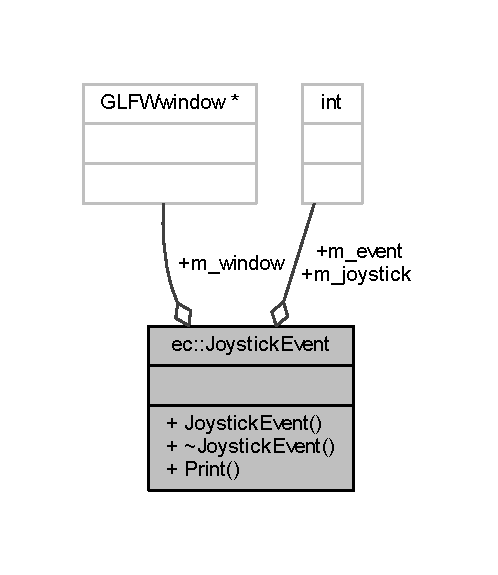
\includegraphics[width=239pt]{structec_1_1_joystick_event__coll__graph}
\end{center}
\end{figure}
\subsection*{Public Member Functions}
\begin{DoxyCompactItemize}
\item 
\mbox{\hyperlink{structec_1_1_joystick_event_a04113c84c127415b3937c214b3e6eb92}{Joystick\+Event}} ()
\item 
\mbox{\hyperlink{structec_1_1_joystick_event_ae08b4530293362fa1ecf1446f13e91e7}{Joystick\+Event}} (G\+L\+F\+Wwindow $\ast$window, int \mbox{\hyperlink{namespaceec_a48a4c5a1e957c8419028491291e37634}{joystick}}, int event)
\item 
\mbox{\hyperlink{structec_1_1_joystick_event_a182ea7dcfcd2e363909eb8ea63a41df8}{$\sim$\+Joystick\+Event}} ()
\item 
void \mbox{\hyperlink{structec_1_1_joystick_event_a8fe710e92962e5b7376167deeac260d7}{print}} () const
\end{DoxyCompactItemize}
\subsection*{Public Attributes}
\begin{DoxyCompactItemize}
\item 
G\+L\+F\+Wwindow $\ast$ \mbox{\hyperlink{structec_1_1_joystick_event_a9b108de0a7db9268dd11642a203ef816}{m\+\_\+window}}
\item 
int \mbox{\hyperlink{structec_1_1_joystick_event_a415b6d2d801b41db8f3dee6b2be35448}{m\+\_\+joystick}}
\item 
int \mbox{\hyperlink{structec_1_1_joystick_event_acf4361edcb473cbf0567137224c86f2a}{m\+\_\+event}}
\end{DoxyCompactItemize}


\subsection{Detailed Description}
An event generated by joystick interaction. 

\subsection{Constructor \& Destructor Documentation}
\mbox{\Hypertarget{structec_1_1_joystick_event_a04113c84c127415b3937c214b3e6eb92}\label{structec_1_1_joystick_event_a04113c84c127415b3937c214b3e6eb92}} 
\index{ec\+::\+Joystick\+Event@{ec\+::\+Joystick\+Event}!Joystick\+Event@{Joystick\+Event}}
\index{Joystick\+Event@{Joystick\+Event}!ec\+::\+Joystick\+Event@{ec\+::\+Joystick\+Event}}
\subsubsection{\texorpdfstring{Joystick\+Event()}{JoystickEvent()}\hspace{0.1cm}{\footnotesize\ttfamily [1/2]}}
{\footnotesize\ttfamily ec\+::\+Joystick\+Event\+::\+Joystick\+Event (\begin{DoxyParamCaption}{ }\end{DoxyParamCaption})\hspace{0.3cm}{\ttfamily [explicit]}}

\mbox{\Hypertarget{structec_1_1_joystick_event_ae08b4530293362fa1ecf1446f13e91e7}\label{structec_1_1_joystick_event_ae08b4530293362fa1ecf1446f13e91e7}} 
\index{ec\+::\+Joystick\+Event@{ec\+::\+Joystick\+Event}!Joystick\+Event@{Joystick\+Event}}
\index{Joystick\+Event@{Joystick\+Event}!ec\+::\+Joystick\+Event@{ec\+::\+Joystick\+Event}}
\subsubsection{\texorpdfstring{Joystick\+Event()}{JoystickEvent()}\hspace{0.1cm}{\footnotesize\ttfamily [2/2]}}
{\footnotesize\ttfamily ec\+::\+Joystick\+Event\+::\+Joystick\+Event (\begin{DoxyParamCaption}\item[{G\+L\+F\+Wwindow $\ast$}]{window,  }\item[{int}]{joystick,  }\item[{int}]{event }\end{DoxyParamCaption})\hspace{0.3cm}{\ttfamily [explicit]}}

\mbox{\Hypertarget{structec_1_1_joystick_event_a182ea7dcfcd2e363909eb8ea63a41df8}\label{structec_1_1_joystick_event_a182ea7dcfcd2e363909eb8ea63a41df8}} 
\index{ec\+::\+Joystick\+Event@{ec\+::\+Joystick\+Event}!````~Joystick\+Event@{$\sim$\+Joystick\+Event}}
\index{````~Joystick\+Event@{$\sim$\+Joystick\+Event}!ec\+::\+Joystick\+Event@{ec\+::\+Joystick\+Event}}
\subsubsection{\texorpdfstring{$\sim$\+Joystick\+Event()}{~JoystickEvent()}}
{\footnotesize\ttfamily ec\+::\+Joystick\+Event\+::$\sim$\+Joystick\+Event (\begin{DoxyParamCaption}{ }\end{DoxyParamCaption})\hspace{0.3cm}{\ttfamily [default]}}



\subsection{Member Function Documentation}
\mbox{\Hypertarget{structec_1_1_joystick_event_a8fe710e92962e5b7376167deeac260d7}\label{structec_1_1_joystick_event_a8fe710e92962e5b7376167deeac260d7}} 
\index{ec\+::\+Joystick\+Event@{ec\+::\+Joystick\+Event}!print@{print}}
\index{print@{print}!ec\+::\+Joystick\+Event@{ec\+::\+Joystick\+Event}}
\subsubsection{\texorpdfstring{print()}{print()}}
{\footnotesize\ttfamily void ec\+::\+Joystick\+Event\+::print (\begin{DoxyParamCaption}{ }\end{DoxyParamCaption}) const}



\subsection{Member Data Documentation}
\mbox{\Hypertarget{structec_1_1_joystick_event_acf4361edcb473cbf0567137224c86f2a}\label{structec_1_1_joystick_event_acf4361edcb473cbf0567137224c86f2a}} 
\index{ec\+::\+Joystick\+Event@{ec\+::\+Joystick\+Event}!m\+\_\+event@{m\+\_\+event}}
\index{m\+\_\+event@{m\+\_\+event}!ec\+::\+Joystick\+Event@{ec\+::\+Joystick\+Event}}
\subsubsection{\texorpdfstring{m\+\_\+event}{m\_event}}
{\footnotesize\ttfamily int ec\+::\+Joystick\+Event\+::m\+\_\+event}

\mbox{\Hypertarget{structec_1_1_joystick_event_a415b6d2d801b41db8f3dee6b2be35448}\label{structec_1_1_joystick_event_a415b6d2d801b41db8f3dee6b2be35448}} 
\index{ec\+::\+Joystick\+Event@{ec\+::\+Joystick\+Event}!m\+\_\+joystick@{m\+\_\+joystick}}
\index{m\+\_\+joystick@{m\+\_\+joystick}!ec\+::\+Joystick\+Event@{ec\+::\+Joystick\+Event}}
\subsubsection{\texorpdfstring{m\+\_\+joystick}{m\_joystick}}
{\footnotesize\ttfamily int ec\+::\+Joystick\+Event\+::m\+\_\+joystick}

\mbox{\Hypertarget{structec_1_1_joystick_event_a9b108de0a7db9268dd11642a203ef816}\label{structec_1_1_joystick_event_a9b108de0a7db9268dd11642a203ef816}} 
\index{ec\+::\+Joystick\+Event@{ec\+::\+Joystick\+Event}!m\+\_\+window@{m\+\_\+window}}
\index{m\+\_\+window@{m\+\_\+window}!ec\+::\+Joystick\+Event@{ec\+::\+Joystick\+Event}}
\subsubsection{\texorpdfstring{m\+\_\+window}{m\_window}}
{\footnotesize\ttfamily G\+L\+F\+Wwindow$\ast$ ec\+::\+Joystick\+Event\+::m\+\_\+window}



The documentation for this struct was generated from the following files\+:\begin{DoxyCompactItemize}
\item 
C\+:/\+Library/\+Job/\+Projekte/\+Simulation\+Visualization/\+Eye\+Candy3\+D/\+Eye\+Candy3\+D/include/\+E\+C3\+D/\+Core/\mbox{\hyperlink{_input_event_8h}{Input\+Event.\+h}}\item 
C\+:/\+Library/\+Job/\+Projekte/\+Simulation\+Visualization/\+Eye\+Candy3\+D/\+Eye\+Candy3\+D/src/\+Core/\mbox{\hyperlink{_input_event_8cpp}{Input\+Event.\+cpp}}\end{DoxyCompactItemize}

\hypertarget{structec_1_1_key_event}{}\section{ec\+:\+:Key\+Event Struct Reference}
\label{structec_1_1_key_event}\index{ec\+::\+Key\+Event@{ec\+::\+Key\+Event}}


{\ttfamily \#include $<$Input\+Event.\+h$>$}



Collaboration diagram for ec\+:\+:Key\+Event\+:\nopagebreak
\begin{figure}[H]
\begin{center}
\leavevmode
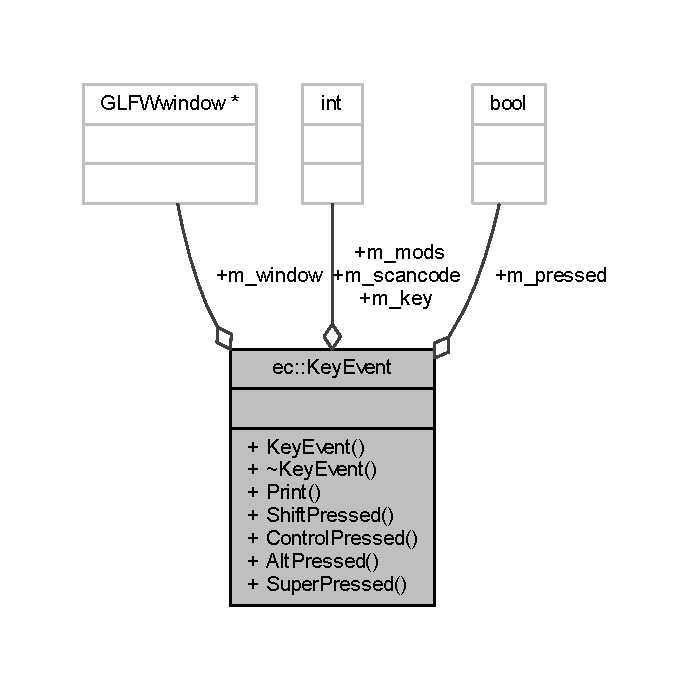
\includegraphics[width=333pt]{structec_1_1_key_event__coll__graph}
\end{center}
\end{figure}
\subsection*{Public Member Functions}
\begin{DoxyCompactItemize}
\item 
\mbox{\hyperlink{structec_1_1_key_event_a679ba7a0050b6514a3a6a110b4128562}{Key\+Event}} (G\+L\+F\+Wwindow $\ast$window, const int key, const int scancode, const int mods, const bool pressed)
\item 
\mbox{\hyperlink{structec_1_1_key_event_a2e9713c01afb046dc2504f17ce42e386}{$\sim$\+Key\+Event}} ()
\item 
void \mbox{\hyperlink{structec_1_1_key_event_ae57433e16a6e51ca2fe57a41de0cf370}{Print}} () const
\item 
bool \mbox{\hyperlink{structec_1_1_key_event_af8fb773cf9944c9ef22be92b4cf68062}{Shift\+Pressed}} () const
\item 
bool \mbox{\hyperlink{structec_1_1_key_event_af80f845419fb29c9b47a13cd7354bc27}{Control\+Pressed}} () const
\item 
bool \mbox{\hyperlink{structec_1_1_key_event_a6881e3dfbb485fdaed76e78663c7a106}{Alt\+Pressed}} () const
\item 
bool \mbox{\hyperlink{structec_1_1_key_event_ac6af6ede353055619a6f7c14b83918cc}{Super\+Pressed}} () const
\end{DoxyCompactItemize}
\subsection*{Public Attributes}
\begin{DoxyCompactItemize}
\item 
G\+L\+F\+Wwindow $\ast$ \mbox{\hyperlink{structec_1_1_key_event_a334f32a8102f1d155a6fec87375efd04}{m\+\_\+window}}
\item 
int \mbox{\hyperlink{structec_1_1_key_event_a1c81390df89a4894405bee6cb101649e}{m\+\_\+key}}
\item 
int \mbox{\hyperlink{structec_1_1_key_event_ac7d1cc5ce7aad43f0aa73879677ad375}{m\+\_\+scancode}}
\item 
int \mbox{\hyperlink{structec_1_1_key_event_a2b57c4779afbd78542be4cee2cd3dcbb}{m\+\_\+mods}}
\item 
bool \mbox{\hyperlink{structec_1_1_key_event_a4e9ab83e1535c1ee34c9eb54c21b05e3}{m\+\_\+pressed}}
\end{DoxyCompactItemize}


\subsection{Constructor \& Destructor Documentation}
\mbox{\Hypertarget{structec_1_1_key_event_a679ba7a0050b6514a3a6a110b4128562}\label{structec_1_1_key_event_a679ba7a0050b6514a3a6a110b4128562}} 
\index{ec\+::\+Key\+Event@{ec\+::\+Key\+Event}!Key\+Event@{Key\+Event}}
\index{Key\+Event@{Key\+Event}!ec\+::\+Key\+Event@{ec\+::\+Key\+Event}}
\subsubsection{\texorpdfstring{Key\+Event()}{KeyEvent()}}
{\footnotesize\ttfamily ec\+::\+Key\+Event\+::\+Key\+Event (\begin{DoxyParamCaption}\item[{G\+L\+F\+Wwindow $\ast$}]{window,  }\item[{const int}]{key,  }\item[{const int}]{scancode,  }\item[{const int}]{mods,  }\item[{const bool}]{pressed }\end{DoxyParamCaption})}

\mbox{\Hypertarget{structec_1_1_key_event_a2e9713c01afb046dc2504f17ce42e386}\label{structec_1_1_key_event_a2e9713c01afb046dc2504f17ce42e386}} 
\index{ec\+::\+Key\+Event@{ec\+::\+Key\+Event}!````~Key\+Event@{$\sim$\+Key\+Event}}
\index{````~Key\+Event@{$\sim$\+Key\+Event}!ec\+::\+Key\+Event@{ec\+::\+Key\+Event}}
\subsubsection{\texorpdfstring{$\sim$\+Key\+Event()}{~KeyEvent()}}
{\footnotesize\ttfamily ec\+::\+Key\+Event\+::$\sim$\+Key\+Event (\begin{DoxyParamCaption}{ }\end{DoxyParamCaption})}



\subsection{Member Function Documentation}
\mbox{\Hypertarget{structec_1_1_key_event_a6881e3dfbb485fdaed76e78663c7a106}\label{structec_1_1_key_event_a6881e3dfbb485fdaed76e78663c7a106}} 
\index{ec\+::\+Key\+Event@{ec\+::\+Key\+Event}!Alt\+Pressed@{Alt\+Pressed}}
\index{Alt\+Pressed@{Alt\+Pressed}!ec\+::\+Key\+Event@{ec\+::\+Key\+Event}}
\subsubsection{\texorpdfstring{Alt\+Pressed()}{AltPressed()}}
{\footnotesize\ttfamily bool ec\+::\+Key\+Event\+::\+Alt\+Pressed (\begin{DoxyParamCaption}{ }\end{DoxyParamCaption}) const}

\mbox{\Hypertarget{structec_1_1_key_event_af80f845419fb29c9b47a13cd7354bc27}\label{structec_1_1_key_event_af80f845419fb29c9b47a13cd7354bc27}} 
\index{ec\+::\+Key\+Event@{ec\+::\+Key\+Event}!Control\+Pressed@{Control\+Pressed}}
\index{Control\+Pressed@{Control\+Pressed}!ec\+::\+Key\+Event@{ec\+::\+Key\+Event}}
\subsubsection{\texorpdfstring{Control\+Pressed()}{ControlPressed()}}
{\footnotesize\ttfamily bool ec\+::\+Key\+Event\+::\+Control\+Pressed (\begin{DoxyParamCaption}{ }\end{DoxyParamCaption}) const}

\mbox{\Hypertarget{structec_1_1_key_event_ae57433e16a6e51ca2fe57a41de0cf370}\label{structec_1_1_key_event_ae57433e16a6e51ca2fe57a41de0cf370}} 
\index{ec\+::\+Key\+Event@{ec\+::\+Key\+Event}!Print@{Print}}
\index{Print@{Print}!ec\+::\+Key\+Event@{ec\+::\+Key\+Event}}
\subsubsection{\texorpdfstring{Print()}{Print()}}
{\footnotesize\ttfamily void ec\+::\+Key\+Event\+::\+Print (\begin{DoxyParamCaption}{ }\end{DoxyParamCaption}) const}

\mbox{\Hypertarget{structec_1_1_key_event_af8fb773cf9944c9ef22be92b4cf68062}\label{structec_1_1_key_event_af8fb773cf9944c9ef22be92b4cf68062}} 
\index{ec\+::\+Key\+Event@{ec\+::\+Key\+Event}!Shift\+Pressed@{Shift\+Pressed}}
\index{Shift\+Pressed@{Shift\+Pressed}!ec\+::\+Key\+Event@{ec\+::\+Key\+Event}}
\subsubsection{\texorpdfstring{Shift\+Pressed()}{ShiftPressed()}}
{\footnotesize\ttfamily bool ec\+::\+Key\+Event\+::\+Shift\+Pressed (\begin{DoxyParamCaption}{ }\end{DoxyParamCaption}) const}

\mbox{\Hypertarget{structec_1_1_key_event_ac6af6ede353055619a6f7c14b83918cc}\label{structec_1_1_key_event_ac6af6ede353055619a6f7c14b83918cc}} 
\index{ec\+::\+Key\+Event@{ec\+::\+Key\+Event}!Super\+Pressed@{Super\+Pressed}}
\index{Super\+Pressed@{Super\+Pressed}!ec\+::\+Key\+Event@{ec\+::\+Key\+Event}}
\subsubsection{\texorpdfstring{Super\+Pressed()}{SuperPressed()}}
{\footnotesize\ttfamily bool ec\+::\+Key\+Event\+::\+Super\+Pressed (\begin{DoxyParamCaption}{ }\end{DoxyParamCaption}) const}



\subsection{Member Data Documentation}
\mbox{\Hypertarget{structec_1_1_key_event_a1c81390df89a4894405bee6cb101649e}\label{structec_1_1_key_event_a1c81390df89a4894405bee6cb101649e}} 
\index{ec\+::\+Key\+Event@{ec\+::\+Key\+Event}!m\+\_\+key@{m\+\_\+key}}
\index{m\+\_\+key@{m\+\_\+key}!ec\+::\+Key\+Event@{ec\+::\+Key\+Event}}
\subsubsection{\texorpdfstring{m\+\_\+key}{m\_key}}
{\footnotesize\ttfamily int ec\+::\+Key\+Event\+::m\+\_\+key}

\mbox{\Hypertarget{structec_1_1_key_event_a2b57c4779afbd78542be4cee2cd3dcbb}\label{structec_1_1_key_event_a2b57c4779afbd78542be4cee2cd3dcbb}} 
\index{ec\+::\+Key\+Event@{ec\+::\+Key\+Event}!m\+\_\+mods@{m\+\_\+mods}}
\index{m\+\_\+mods@{m\+\_\+mods}!ec\+::\+Key\+Event@{ec\+::\+Key\+Event}}
\subsubsection{\texorpdfstring{m\+\_\+mods}{m\_mods}}
{\footnotesize\ttfamily int ec\+::\+Key\+Event\+::m\+\_\+mods}

\mbox{\Hypertarget{structec_1_1_key_event_a4e9ab83e1535c1ee34c9eb54c21b05e3}\label{structec_1_1_key_event_a4e9ab83e1535c1ee34c9eb54c21b05e3}} 
\index{ec\+::\+Key\+Event@{ec\+::\+Key\+Event}!m\+\_\+pressed@{m\+\_\+pressed}}
\index{m\+\_\+pressed@{m\+\_\+pressed}!ec\+::\+Key\+Event@{ec\+::\+Key\+Event}}
\subsubsection{\texorpdfstring{m\+\_\+pressed}{m\_pressed}}
{\footnotesize\ttfamily bool ec\+::\+Key\+Event\+::m\+\_\+pressed}

\mbox{\Hypertarget{structec_1_1_key_event_ac7d1cc5ce7aad43f0aa73879677ad375}\label{structec_1_1_key_event_ac7d1cc5ce7aad43f0aa73879677ad375}} 
\index{ec\+::\+Key\+Event@{ec\+::\+Key\+Event}!m\+\_\+scancode@{m\+\_\+scancode}}
\index{m\+\_\+scancode@{m\+\_\+scancode}!ec\+::\+Key\+Event@{ec\+::\+Key\+Event}}
\subsubsection{\texorpdfstring{m\+\_\+scancode}{m\_scancode}}
{\footnotesize\ttfamily int ec\+::\+Key\+Event\+::m\+\_\+scancode}

\mbox{\Hypertarget{structec_1_1_key_event_a334f32a8102f1d155a6fec87375efd04}\label{structec_1_1_key_event_a334f32a8102f1d155a6fec87375efd04}} 
\index{ec\+::\+Key\+Event@{ec\+::\+Key\+Event}!m\+\_\+window@{m\+\_\+window}}
\index{m\+\_\+window@{m\+\_\+window}!ec\+::\+Key\+Event@{ec\+::\+Key\+Event}}
\subsubsection{\texorpdfstring{m\+\_\+window}{m\_window}}
{\footnotesize\ttfamily G\+L\+F\+Wwindow$\ast$ ec\+::\+Key\+Event\+::m\+\_\+window}



The documentation for this struct was generated from the following files\+:\begin{DoxyCompactItemize}
\item 
D\+:/\+Library/\+Documents/\+Job/\+Forschungsmaster/\+Projekte/\+Eye\+Candy3\+D/\+Eye\+Candy3\+D/include/\+E\+C3\+D/\+Core/\mbox{\hyperlink{_input_event_8h}{Input\+Event.\+h}}\item 
D\+:/\+Library/\+Documents/\+Job/\+Forschungsmaster/\+Projekte/\+Eye\+Candy3\+D/\+Eye\+Candy3\+D/src/\+Core/\mbox{\hyperlink{_input_event_8cpp}{Input\+Event.\+cpp}}\end{DoxyCompactItemize}

\hypertarget{classec_1_1_material}{}\section{ec\+:\+:Material Class Reference}
\label{classec_1_1_material}\index{ec\+::\+Material@{ec\+::\+Material}}


{\ttfamily \#include $<$Material.\+h$>$}



Collaboration diagram for ec\+:\+:Material\+:\nopagebreak
\begin{figure}[H]
\begin{center}
\leavevmode
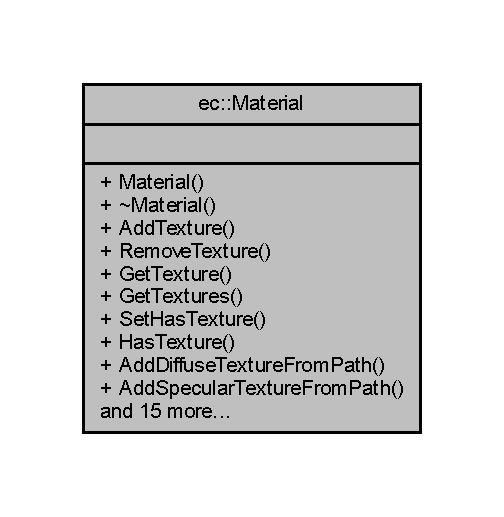
\includegraphics[width=232pt]{classec_1_1_material__coll__graph}
\end{center}
\end{figure}
\subsection*{Public Member Functions}
\begin{DoxyCompactItemize}
\item 
\mbox{\hyperlink{classec_1_1_material_a259d88ca352df2d284380f0b37052652}{Material}} ()
\item 
virtual \mbox{\hyperlink{classec_1_1_material_aec5bd3f3ef761f49a5028b415a9de52e}{$\sim$\+Material}} ()
\item 
void \mbox{\hyperlink{classec_1_1_material_aad92ada3fcc1f7b66e6bf3b6aeac73b8}{add\+Texture}} (const \mbox{\hyperlink{classec_1_1_texture}{Texture}} \&texture)
\item 
void \mbox{\hyperlink{classec_1_1_material_a83a673bcbcdef42bcea99939e5d6ff03}{remove\+Texture}} (const \mbox{\hyperlink{classec_1_1_texture}{Texture}} \&texture)
\item 
\mbox{\hyperlink{classec_1_1_texture}{Texture}} $\ast$ \mbox{\hyperlink{classec_1_1_material_a8679615f24284e809f213b882bec81bf}{get\+Texture}} (unsigned int index)
\item 
const std\+::vector$<$ \mbox{\hyperlink{classec_1_1_texture}{Texture}} $>$ \& \mbox{\hyperlink{classec_1_1_material_a95d74f12ec9d69a764a249e36b6b857c}{get\+Textures}} () const
\item 
bool \mbox{\hyperlink{classec_1_1_material_a961612ff2caee16d5d4b8f9b74042cf2}{has\+Texture}} () const
\item 
bool \mbox{\hyperlink{classec_1_1_material_a15b5c4adb903b16c25ad312963027924}{add\+Diffuse\+Texture\+From\+Path}} (const char $\ast$path)
\item 
void \mbox{\hyperlink{classec_1_1_material_afdd82441b5b2168161a17824e4a90f6f}{set\+Color\+Ambient}} (const glm\+::vec4 \&color)
\item 
void \mbox{\hyperlink{classec_1_1_material_a4ee41422a7625ac8a9f8a5e52bb18cf7}{set\+Color\+Ambient}} (float r, float g, float b, float a)
\item 
void \mbox{\hyperlink{classec_1_1_material_a22b711323a849e2ff6f9ffb871402a3e}{set\+Color\+Diffuse}} (const glm\+::vec4 \&color)
\item 
void \mbox{\hyperlink{classec_1_1_material_aa86e76b930ffffd45076465eff08bf27}{set\+Color\+Diffuse}} (float r, float g, float b, float a)
\item 
void \mbox{\hyperlink{classec_1_1_material_a947f0946ff806852e1733b1e95a03489}{set\+Color\+Specular}} (const glm\+::vec4 \&color)
\item 
void \mbox{\hyperlink{classec_1_1_material_aa62e40f0571c25eb097f03c74849f918}{set\+Color\+Specular}} (float r, float g, float b, float a)
\item 
void \mbox{\hyperlink{classec_1_1_material_a77ac7702af54e4c8a7301387bea159dd}{set\+Color\+Emission}} (const glm\+::vec4 \&color)
\item 
void \mbox{\hyperlink{classec_1_1_material_a6fa0dfb1c76b2c9b07fbd2b28021010c}{set\+Color\+Emission}} (float r, float g, float b, float a)
\item 
const glm\+::vec4 \& \mbox{\hyperlink{classec_1_1_material_a68e143f6390ae7e9bc6c080853191f94}{get\+Color\+Ambient}} () const
\item 
const glm\+::vec4 \& \mbox{\hyperlink{classec_1_1_material_a6156c82b63756da91d013b5eb39fccf5}{get\+Color\+Diffuse}} () const
\item 
const glm\+::vec4 \& \mbox{\hyperlink{classec_1_1_material_a0a4a766b22c9adeffdff5c0d5140167e}{get\+Color\+Specular}} () const
\item 
const glm\+::vec4 \& \mbox{\hyperlink{classec_1_1_material_af6a4a55683956cd0b06d0a8de1dc4b9f}{get\+Color\+Emission}} () const
\item 
void \mbox{\hyperlink{classec_1_1_material_a4b9efb15466a547d4579566dfb1e558f}{set\+Shininess}} (float shininess)
\item 
float \mbox{\hyperlink{classec_1_1_material_a125ba490c4191f8f6fe77e76934ed33a}{get\+Shininess}} () const
\end{DoxyCompactItemize}


\subsection{Constructor \& Destructor Documentation}
\mbox{\Hypertarget{classec_1_1_material_a259d88ca352df2d284380f0b37052652}\label{classec_1_1_material_a259d88ca352df2d284380f0b37052652}} 
\index{ec\+::\+Material@{ec\+::\+Material}!Material@{Material}}
\index{Material@{Material}!ec\+::\+Material@{ec\+::\+Material}}
\subsubsection{\texorpdfstring{Material()}{Material()}}
{\footnotesize\ttfamily ec\+::\+Material\+::\+Material (\begin{DoxyParamCaption}{ }\end{DoxyParamCaption})\hspace{0.3cm}{\ttfamily [explicit]}}

\mbox{\Hypertarget{classec_1_1_material_aec5bd3f3ef761f49a5028b415a9de52e}\label{classec_1_1_material_aec5bd3f3ef761f49a5028b415a9de52e}} 
\index{ec\+::\+Material@{ec\+::\+Material}!````~Material@{$\sim$\+Material}}
\index{````~Material@{$\sim$\+Material}!ec\+::\+Material@{ec\+::\+Material}}
\subsubsection{\texorpdfstring{$\sim$\+Material()}{~Material()}}
{\footnotesize\ttfamily ec\+::\+Material\+::$\sim$\+Material (\begin{DoxyParamCaption}{ }\end{DoxyParamCaption})\hspace{0.3cm}{\ttfamily [virtual]}, {\ttfamily [default]}}



\subsection{Member Function Documentation}
\mbox{\Hypertarget{classec_1_1_material_a15b5c4adb903b16c25ad312963027924}\label{classec_1_1_material_a15b5c4adb903b16c25ad312963027924}} 
\index{ec\+::\+Material@{ec\+::\+Material}!add\+Diffuse\+Texture\+From\+Path@{add\+Diffuse\+Texture\+From\+Path}}
\index{add\+Diffuse\+Texture\+From\+Path@{add\+Diffuse\+Texture\+From\+Path}!ec\+::\+Material@{ec\+::\+Material}}
\subsubsection{\texorpdfstring{add\+Diffuse\+Texture\+From\+Path()}{addDiffuseTextureFromPath()}}
{\footnotesize\ttfamily bool ec\+::\+Material\+::add\+Diffuse\+Texture\+From\+Path (\begin{DoxyParamCaption}\item[{const char $\ast$}]{path }\end{DoxyParamCaption})}

\mbox{\Hypertarget{classec_1_1_material_aad92ada3fcc1f7b66e6bf3b6aeac73b8}\label{classec_1_1_material_aad92ada3fcc1f7b66e6bf3b6aeac73b8}} 
\index{ec\+::\+Material@{ec\+::\+Material}!add\+Texture@{add\+Texture}}
\index{add\+Texture@{add\+Texture}!ec\+::\+Material@{ec\+::\+Material}}
\subsubsection{\texorpdfstring{add\+Texture()}{addTexture()}}
{\footnotesize\ttfamily void ec\+::\+Material\+::add\+Texture (\begin{DoxyParamCaption}\item[{const \mbox{\hyperlink{classec_1_1_texture}{Texture}} \&}]{texture }\end{DoxyParamCaption})}

\mbox{\Hypertarget{classec_1_1_material_a68e143f6390ae7e9bc6c080853191f94}\label{classec_1_1_material_a68e143f6390ae7e9bc6c080853191f94}} 
\index{ec\+::\+Material@{ec\+::\+Material}!get\+Color\+Ambient@{get\+Color\+Ambient}}
\index{get\+Color\+Ambient@{get\+Color\+Ambient}!ec\+::\+Material@{ec\+::\+Material}}
\subsubsection{\texorpdfstring{get\+Color\+Ambient()}{getColorAmbient()}}
{\footnotesize\ttfamily const glm\+::vec4 \& ec\+::\+Material\+::get\+Color\+Ambient (\begin{DoxyParamCaption}{ }\end{DoxyParamCaption}) const}

\mbox{\Hypertarget{classec_1_1_material_a6156c82b63756da91d013b5eb39fccf5}\label{classec_1_1_material_a6156c82b63756da91d013b5eb39fccf5}} 
\index{ec\+::\+Material@{ec\+::\+Material}!get\+Color\+Diffuse@{get\+Color\+Diffuse}}
\index{get\+Color\+Diffuse@{get\+Color\+Diffuse}!ec\+::\+Material@{ec\+::\+Material}}
\subsubsection{\texorpdfstring{get\+Color\+Diffuse()}{getColorDiffuse()}}
{\footnotesize\ttfamily const glm\+::vec4 \& ec\+::\+Material\+::get\+Color\+Diffuse (\begin{DoxyParamCaption}{ }\end{DoxyParamCaption}) const}

\mbox{\Hypertarget{classec_1_1_material_af6a4a55683956cd0b06d0a8de1dc4b9f}\label{classec_1_1_material_af6a4a55683956cd0b06d0a8de1dc4b9f}} 
\index{ec\+::\+Material@{ec\+::\+Material}!get\+Color\+Emission@{get\+Color\+Emission}}
\index{get\+Color\+Emission@{get\+Color\+Emission}!ec\+::\+Material@{ec\+::\+Material}}
\subsubsection{\texorpdfstring{get\+Color\+Emission()}{getColorEmission()}}
{\footnotesize\ttfamily const glm\+::vec4 \& ec\+::\+Material\+::get\+Color\+Emission (\begin{DoxyParamCaption}{ }\end{DoxyParamCaption}) const}

\mbox{\Hypertarget{classec_1_1_material_a0a4a766b22c9adeffdff5c0d5140167e}\label{classec_1_1_material_a0a4a766b22c9adeffdff5c0d5140167e}} 
\index{ec\+::\+Material@{ec\+::\+Material}!get\+Color\+Specular@{get\+Color\+Specular}}
\index{get\+Color\+Specular@{get\+Color\+Specular}!ec\+::\+Material@{ec\+::\+Material}}
\subsubsection{\texorpdfstring{get\+Color\+Specular()}{getColorSpecular()}}
{\footnotesize\ttfamily const glm\+::vec4 \& ec\+::\+Material\+::get\+Color\+Specular (\begin{DoxyParamCaption}{ }\end{DoxyParamCaption}) const}

\mbox{\Hypertarget{classec_1_1_material_a125ba490c4191f8f6fe77e76934ed33a}\label{classec_1_1_material_a125ba490c4191f8f6fe77e76934ed33a}} 
\index{ec\+::\+Material@{ec\+::\+Material}!get\+Shininess@{get\+Shininess}}
\index{get\+Shininess@{get\+Shininess}!ec\+::\+Material@{ec\+::\+Material}}
\subsubsection{\texorpdfstring{get\+Shininess()}{getShininess()}}
{\footnotesize\ttfamily float ec\+::\+Material\+::get\+Shininess (\begin{DoxyParamCaption}{ }\end{DoxyParamCaption}) const}

\mbox{\Hypertarget{classec_1_1_material_a8679615f24284e809f213b882bec81bf}\label{classec_1_1_material_a8679615f24284e809f213b882bec81bf}} 
\index{ec\+::\+Material@{ec\+::\+Material}!get\+Texture@{get\+Texture}}
\index{get\+Texture@{get\+Texture}!ec\+::\+Material@{ec\+::\+Material}}
\subsubsection{\texorpdfstring{get\+Texture()}{getTexture()}}
{\footnotesize\ttfamily \mbox{\hyperlink{classec_1_1_texture}{ec\+::\+Texture}} $\ast$ ec\+::\+Material\+::get\+Texture (\begin{DoxyParamCaption}\item[{unsigned int}]{index }\end{DoxyParamCaption})}

\mbox{\Hypertarget{classec_1_1_material_a95d74f12ec9d69a764a249e36b6b857c}\label{classec_1_1_material_a95d74f12ec9d69a764a249e36b6b857c}} 
\index{ec\+::\+Material@{ec\+::\+Material}!get\+Textures@{get\+Textures}}
\index{get\+Textures@{get\+Textures}!ec\+::\+Material@{ec\+::\+Material}}
\subsubsection{\texorpdfstring{get\+Textures()}{getTextures()}}
{\footnotesize\ttfamily const std\+::vector$<$ \mbox{\hyperlink{classec_1_1_texture}{Texture}} $>$ \& ec\+::\+Material\+::get\+Textures (\begin{DoxyParamCaption}{ }\end{DoxyParamCaption}) const}

\mbox{\Hypertarget{classec_1_1_material_a961612ff2caee16d5d4b8f9b74042cf2}\label{classec_1_1_material_a961612ff2caee16d5d4b8f9b74042cf2}} 
\index{ec\+::\+Material@{ec\+::\+Material}!has\+Texture@{has\+Texture}}
\index{has\+Texture@{has\+Texture}!ec\+::\+Material@{ec\+::\+Material}}
\subsubsection{\texorpdfstring{has\+Texture()}{hasTexture()}}
{\footnotesize\ttfamily bool ec\+::\+Material\+::has\+Texture (\begin{DoxyParamCaption}{ }\end{DoxyParamCaption}) const}

\mbox{\Hypertarget{classec_1_1_material_a83a673bcbcdef42bcea99939e5d6ff03}\label{classec_1_1_material_a83a673bcbcdef42bcea99939e5d6ff03}} 
\index{ec\+::\+Material@{ec\+::\+Material}!remove\+Texture@{remove\+Texture}}
\index{remove\+Texture@{remove\+Texture}!ec\+::\+Material@{ec\+::\+Material}}
\subsubsection{\texorpdfstring{remove\+Texture()}{removeTexture()}}
{\footnotesize\ttfamily void ec\+::\+Material\+::remove\+Texture (\begin{DoxyParamCaption}\item[{const \mbox{\hyperlink{classec_1_1_texture}{Texture}} \&}]{texture }\end{DoxyParamCaption})}

\mbox{\Hypertarget{classec_1_1_material_afdd82441b5b2168161a17824e4a90f6f}\label{classec_1_1_material_afdd82441b5b2168161a17824e4a90f6f}} 
\index{ec\+::\+Material@{ec\+::\+Material}!set\+Color\+Ambient@{set\+Color\+Ambient}}
\index{set\+Color\+Ambient@{set\+Color\+Ambient}!ec\+::\+Material@{ec\+::\+Material}}
\subsubsection{\texorpdfstring{set\+Color\+Ambient()}{setColorAmbient()}\hspace{0.1cm}{\footnotesize\ttfamily [1/2]}}
{\footnotesize\ttfamily void ec\+::\+Material\+::set\+Color\+Ambient (\begin{DoxyParamCaption}\item[{const glm\+::vec4 \&}]{color }\end{DoxyParamCaption})}

\mbox{\Hypertarget{classec_1_1_material_a4ee41422a7625ac8a9f8a5e52bb18cf7}\label{classec_1_1_material_a4ee41422a7625ac8a9f8a5e52bb18cf7}} 
\index{ec\+::\+Material@{ec\+::\+Material}!set\+Color\+Ambient@{set\+Color\+Ambient}}
\index{set\+Color\+Ambient@{set\+Color\+Ambient}!ec\+::\+Material@{ec\+::\+Material}}
\subsubsection{\texorpdfstring{set\+Color\+Ambient()}{setColorAmbient()}\hspace{0.1cm}{\footnotesize\ttfamily [2/2]}}
{\footnotesize\ttfamily void ec\+::\+Material\+::set\+Color\+Ambient (\begin{DoxyParamCaption}\item[{float}]{r,  }\item[{float}]{g,  }\item[{float}]{b,  }\item[{float}]{a }\end{DoxyParamCaption})}

\mbox{\Hypertarget{classec_1_1_material_a22b711323a849e2ff6f9ffb871402a3e}\label{classec_1_1_material_a22b711323a849e2ff6f9ffb871402a3e}} 
\index{ec\+::\+Material@{ec\+::\+Material}!set\+Color\+Diffuse@{set\+Color\+Diffuse}}
\index{set\+Color\+Diffuse@{set\+Color\+Diffuse}!ec\+::\+Material@{ec\+::\+Material}}
\subsubsection{\texorpdfstring{set\+Color\+Diffuse()}{setColorDiffuse()}\hspace{0.1cm}{\footnotesize\ttfamily [1/2]}}
{\footnotesize\ttfamily void ec\+::\+Material\+::set\+Color\+Diffuse (\begin{DoxyParamCaption}\item[{const glm\+::vec4 \&}]{color }\end{DoxyParamCaption})}

\mbox{\Hypertarget{classec_1_1_material_aa86e76b930ffffd45076465eff08bf27}\label{classec_1_1_material_aa86e76b930ffffd45076465eff08bf27}} 
\index{ec\+::\+Material@{ec\+::\+Material}!set\+Color\+Diffuse@{set\+Color\+Diffuse}}
\index{set\+Color\+Diffuse@{set\+Color\+Diffuse}!ec\+::\+Material@{ec\+::\+Material}}
\subsubsection{\texorpdfstring{set\+Color\+Diffuse()}{setColorDiffuse()}\hspace{0.1cm}{\footnotesize\ttfamily [2/2]}}
{\footnotesize\ttfamily void ec\+::\+Material\+::set\+Color\+Diffuse (\begin{DoxyParamCaption}\item[{float}]{r,  }\item[{float}]{g,  }\item[{float}]{b,  }\item[{float}]{a }\end{DoxyParamCaption})}

\mbox{\Hypertarget{classec_1_1_material_a77ac7702af54e4c8a7301387bea159dd}\label{classec_1_1_material_a77ac7702af54e4c8a7301387bea159dd}} 
\index{ec\+::\+Material@{ec\+::\+Material}!set\+Color\+Emission@{set\+Color\+Emission}}
\index{set\+Color\+Emission@{set\+Color\+Emission}!ec\+::\+Material@{ec\+::\+Material}}
\subsubsection{\texorpdfstring{set\+Color\+Emission()}{setColorEmission()}\hspace{0.1cm}{\footnotesize\ttfamily [1/2]}}
{\footnotesize\ttfamily void ec\+::\+Material\+::set\+Color\+Emission (\begin{DoxyParamCaption}\item[{const glm\+::vec4 \&}]{color }\end{DoxyParamCaption})}

\mbox{\Hypertarget{classec_1_1_material_a6fa0dfb1c76b2c9b07fbd2b28021010c}\label{classec_1_1_material_a6fa0dfb1c76b2c9b07fbd2b28021010c}} 
\index{ec\+::\+Material@{ec\+::\+Material}!set\+Color\+Emission@{set\+Color\+Emission}}
\index{set\+Color\+Emission@{set\+Color\+Emission}!ec\+::\+Material@{ec\+::\+Material}}
\subsubsection{\texorpdfstring{set\+Color\+Emission()}{setColorEmission()}\hspace{0.1cm}{\footnotesize\ttfamily [2/2]}}
{\footnotesize\ttfamily void ec\+::\+Material\+::set\+Color\+Emission (\begin{DoxyParamCaption}\item[{float}]{r,  }\item[{float}]{g,  }\item[{float}]{b,  }\item[{float}]{a }\end{DoxyParamCaption})}

\mbox{\Hypertarget{classec_1_1_material_a947f0946ff806852e1733b1e95a03489}\label{classec_1_1_material_a947f0946ff806852e1733b1e95a03489}} 
\index{ec\+::\+Material@{ec\+::\+Material}!set\+Color\+Specular@{set\+Color\+Specular}}
\index{set\+Color\+Specular@{set\+Color\+Specular}!ec\+::\+Material@{ec\+::\+Material}}
\subsubsection{\texorpdfstring{set\+Color\+Specular()}{setColorSpecular()}\hspace{0.1cm}{\footnotesize\ttfamily [1/2]}}
{\footnotesize\ttfamily void ec\+::\+Material\+::set\+Color\+Specular (\begin{DoxyParamCaption}\item[{const glm\+::vec4 \&}]{color }\end{DoxyParamCaption})}

\mbox{\Hypertarget{classec_1_1_material_aa62e40f0571c25eb097f03c74849f918}\label{classec_1_1_material_aa62e40f0571c25eb097f03c74849f918}} 
\index{ec\+::\+Material@{ec\+::\+Material}!set\+Color\+Specular@{set\+Color\+Specular}}
\index{set\+Color\+Specular@{set\+Color\+Specular}!ec\+::\+Material@{ec\+::\+Material}}
\subsubsection{\texorpdfstring{set\+Color\+Specular()}{setColorSpecular()}\hspace{0.1cm}{\footnotesize\ttfamily [2/2]}}
{\footnotesize\ttfamily void ec\+::\+Material\+::set\+Color\+Specular (\begin{DoxyParamCaption}\item[{float}]{r,  }\item[{float}]{g,  }\item[{float}]{b,  }\item[{float}]{a }\end{DoxyParamCaption})}

\mbox{\Hypertarget{classec_1_1_material_a4b9efb15466a547d4579566dfb1e558f}\label{classec_1_1_material_a4b9efb15466a547d4579566dfb1e558f}} 
\index{ec\+::\+Material@{ec\+::\+Material}!set\+Shininess@{set\+Shininess}}
\index{set\+Shininess@{set\+Shininess}!ec\+::\+Material@{ec\+::\+Material}}
\subsubsection{\texorpdfstring{set\+Shininess()}{setShininess()}}
{\footnotesize\ttfamily void ec\+::\+Material\+::set\+Shininess (\begin{DoxyParamCaption}\item[{float}]{shininess }\end{DoxyParamCaption})}



The documentation for this class was generated from the following files\+:\begin{DoxyCompactItemize}
\item 
D\+:/\+Library/\+Documents/\+Job/\+Forschungsmaster/\+Projekte/\+Simulation\+Visualization/\+Eye\+Candy3\+D/\+Eye\+Candy3\+D/include/\+E\+C3\+D/\+Core/\mbox{\hyperlink{_material_8h}{Material.\+h}}\item 
D\+:/\+Library/\+Documents/\+Job/\+Forschungsmaster/\+Projekte/\+Simulation\+Visualization/\+Eye\+Candy3\+D/\+Eye\+Candy3\+D/src/\+Core/\mbox{\hyperlink{_material_8cpp}{Material.\+cpp}}\end{DoxyCompactItemize}

\hypertarget{structec_1_1_mouse_button_event}{}\section{ec\+:\+:Mouse\+Button\+Event Struct Reference}
\label{structec_1_1_mouse_button_event}\index{ec\+::\+Mouse\+Button\+Event@{ec\+::\+Mouse\+Button\+Event}}


{\ttfamily \#include $<$Input\+Event.\+h$>$}



Collaboration diagram for ec\+:\+:Mouse\+Button\+Event\+:\nopagebreak
\begin{figure}[H]
\begin{center}
\leavevmode
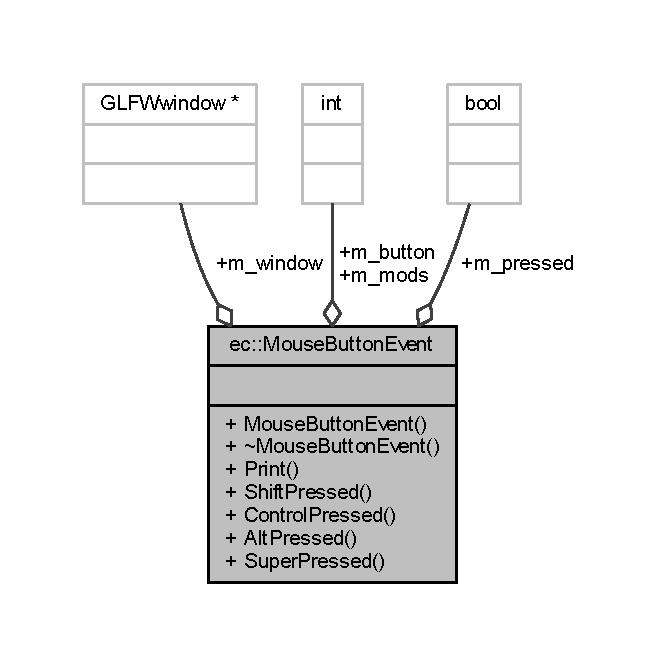
\includegraphics[width=317pt]{structec_1_1_mouse_button_event__coll__graph}
\end{center}
\end{figure}
\subsection*{Public Member Functions}
\begin{DoxyCompactItemize}
\item 
\mbox{\hyperlink{structec_1_1_mouse_button_event_aa7c76016af8d30e5c5486d5249568414}{Mouse\+Button\+Event}} (G\+L\+F\+Wwindow $\ast$window, const int button, const int mods, const bool pressed)
\item 
\mbox{\hyperlink{structec_1_1_mouse_button_event_af4e546257a07f8500dea2b49a79d644d}{$\sim$\+Mouse\+Button\+Event}} ()
\item 
void \mbox{\hyperlink{structec_1_1_mouse_button_event_a6149d796ef4dcd8bfd4540c79f8d6879}{Print}} () const
\item 
bool \mbox{\hyperlink{structec_1_1_mouse_button_event_afcdeea2b5b819f7dd5a82398fe400aca}{Shift\+Pressed}} () const
\item 
bool \mbox{\hyperlink{structec_1_1_mouse_button_event_a47190821b20fc37538379471836aa211}{Control\+Pressed}} () const
\item 
bool \mbox{\hyperlink{structec_1_1_mouse_button_event_a2a63bd0d1b22a8afe549fa49d920643c}{Alt\+Pressed}} () const
\item 
bool \mbox{\hyperlink{structec_1_1_mouse_button_event_a6cedd70bc22c194bcf3b3badeac58551}{Super\+Pressed}} () const
\end{DoxyCompactItemize}
\subsection*{Public Attributes}
\begin{DoxyCompactItemize}
\item 
G\+L\+F\+Wwindow $\ast$ \mbox{\hyperlink{structec_1_1_mouse_button_event_ab83fb7bb5cd28b90c48fd6327fe45f9c}{m\+\_\+window}}
\item 
int \mbox{\hyperlink{structec_1_1_mouse_button_event_a98e02b29b7b5bd6c1923b7b09641ed9e}{m\+\_\+button}}
\item 
int \mbox{\hyperlink{structec_1_1_mouse_button_event_afab73baa804fd9b9ab63846acf2274a9}{m\+\_\+mods}}
\item 
bool \mbox{\hyperlink{structec_1_1_mouse_button_event_ab8a22a5ef68729a7227d60b9b58bd438}{m\+\_\+pressed}}
\end{DoxyCompactItemize}


\subsection{Constructor \& Destructor Documentation}
\mbox{\Hypertarget{structec_1_1_mouse_button_event_aa7c76016af8d30e5c5486d5249568414}\label{structec_1_1_mouse_button_event_aa7c76016af8d30e5c5486d5249568414}} 
\index{ec\+::\+Mouse\+Button\+Event@{ec\+::\+Mouse\+Button\+Event}!Mouse\+Button\+Event@{Mouse\+Button\+Event}}
\index{Mouse\+Button\+Event@{Mouse\+Button\+Event}!ec\+::\+Mouse\+Button\+Event@{ec\+::\+Mouse\+Button\+Event}}
\subsubsection{\texorpdfstring{Mouse\+Button\+Event()}{MouseButtonEvent()}}
{\footnotesize\ttfamily ec\+::\+Mouse\+Button\+Event\+::\+Mouse\+Button\+Event (\begin{DoxyParamCaption}\item[{G\+L\+F\+Wwindow $\ast$}]{window,  }\item[{const int}]{button,  }\item[{const int}]{mods,  }\item[{const bool}]{pressed }\end{DoxyParamCaption})}

\mbox{\Hypertarget{structec_1_1_mouse_button_event_af4e546257a07f8500dea2b49a79d644d}\label{structec_1_1_mouse_button_event_af4e546257a07f8500dea2b49a79d644d}} 
\index{ec\+::\+Mouse\+Button\+Event@{ec\+::\+Mouse\+Button\+Event}!````~Mouse\+Button\+Event@{$\sim$\+Mouse\+Button\+Event}}
\index{````~Mouse\+Button\+Event@{$\sim$\+Mouse\+Button\+Event}!ec\+::\+Mouse\+Button\+Event@{ec\+::\+Mouse\+Button\+Event}}
\subsubsection{\texorpdfstring{$\sim$\+Mouse\+Button\+Event()}{~MouseButtonEvent()}}
{\footnotesize\ttfamily ec\+::\+Mouse\+Button\+Event\+::$\sim$\+Mouse\+Button\+Event (\begin{DoxyParamCaption}{ }\end{DoxyParamCaption})}



\subsection{Member Function Documentation}
\mbox{\Hypertarget{structec_1_1_mouse_button_event_a2a63bd0d1b22a8afe549fa49d920643c}\label{structec_1_1_mouse_button_event_a2a63bd0d1b22a8afe549fa49d920643c}} 
\index{ec\+::\+Mouse\+Button\+Event@{ec\+::\+Mouse\+Button\+Event}!Alt\+Pressed@{Alt\+Pressed}}
\index{Alt\+Pressed@{Alt\+Pressed}!ec\+::\+Mouse\+Button\+Event@{ec\+::\+Mouse\+Button\+Event}}
\subsubsection{\texorpdfstring{Alt\+Pressed()}{AltPressed()}}
{\footnotesize\ttfamily bool ec\+::\+Mouse\+Button\+Event\+::\+Alt\+Pressed (\begin{DoxyParamCaption}{ }\end{DoxyParamCaption}) const}

\mbox{\Hypertarget{structec_1_1_mouse_button_event_a47190821b20fc37538379471836aa211}\label{structec_1_1_mouse_button_event_a47190821b20fc37538379471836aa211}} 
\index{ec\+::\+Mouse\+Button\+Event@{ec\+::\+Mouse\+Button\+Event}!Control\+Pressed@{Control\+Pressed}}
\index{Control\+Pressed@{Control\+Pressed}!ec\+::\+Mouse\+Button\+Event@{ec\+::\+Mouse\+Button\+Event}}
\subsubsection{\texorpdfstring{Control\+Pressed()}{ControlPressed()}}
{\footnotesize\ttfamily bool ec\+::\+Mouse\+Button\+Event\+::\+Control\+Pressed (\begin{DoxyParamCaption}{ }\end{DoxyParamCaption}) const}

\mbox{\Hypertarget{structec_1_1_mouse_button_event_a6149d796ef4dcd8bfd4540c79f8d6879}\label{structec_1_1_mouse_button_event_a6149d796ef4dcd8bfd4540c79f8d6879}} 
\index{ec\+::\+Mouse\+Button\+Event@{ec\+::\+Mouse\+Button\+Event}!Print@{Print}}
\index{Print@{Print}!ec\+::\+Mouse\+Button\+Event@{ec\+::\+Mouse\+Button\+Event}}
\subsubsection{\texorpdfstring{Print()}{Print()}}
{\footnotesize\ttfamily void ec\+::\+Mouse\+Button\+Event\+::\+Print (\begin{DoxyParamCaption}{ }\end{DoxyParamCaption}) const}

\mbox{\Hypertarget{structec_1_1_mouse_button_event_afcdeea2b5b819f7dd5a82398fe400aca}\label{structec_1_1_mouse_button_event_afcdeea2b5b819f7dd5a82398fe400aca}} 
\index{ec\+::\+Mouse\+Button\+Event@{ec\+::\+Mouse\+Button\+Event}!Shift\+Pressed@{Shift\+Pressed}}
\index{Shift\+Pressed@{Shift\+Pressed}!ec\+::\+Mouse\+Button\+Event@{ec\+::\+Mouse\+Button\+Event}}
\subsubsection{\texorpdfstring{Shift\+Pressed()}{ShiftPressed()}}
{\footnotesize\ttfamily bool ec\+::\+Mouse\+Button\+Event\+::\+Shift\+Pressed (\begin{DoxyParamCaption}{ }\end{DoxyParamCaption}) const}

\mbox{\Hypertarget{structec_1_1_mouse_button_event_a6cedd70bc22c194bcf3b3badeac58551}\label{structec_1_1_mouse_button_event_a6cedd70bc22c194bcf3b3badeac58551}} 
\index{ec\+::\+Mouse\+Button\+Event@{ec\+::\+Mouse\+Button\+Event}!Super\+Pressed@{Super\+Pressed}}
\index{Super\+Pressed@{Super\+Pressed}!ec\+::\+Mouse\+Button\+Event@{ec\+::\+Mouse\+Button\+Event}}
\subsubsection{\texorpdfstring{Super\+Pressed()}{SuperPressed()}}
{\footnotesize\ttfamily bool ec\+::\+Mouse\+Button\+Event\+::\+Super\+Pressed (\begin{DoxyParamCaption}{ }\end{DoxyParamCaption}) const}



\subsection{Member Data Documentation}
\mbox{\Hypertarget{structec_1_1_mouse_button_event_a98e02b29b7b5bd6c1923b7b09641ed9e}\label{structec_1_1_mouse_button_event_a98e02b29b7b5bd6c1923b7b09641ed9e}} 
\index{ec\+::\+Mouse\+Button\+Event@{ec\+::\+Mouse\+Button\+Event}!m\+\_\+button@{m\+\_\+button}}
\index{m\+\_\+button@{m\+\_\+button}!ec\+::\+Mouse\+Button\+Event@{ec\+::\+Mouse\+Button\+Event}}
\subsubsection{\texorpdfstring{m\+\_\+button}{m\_button}}
{\footnotesize\ttfamily int ec\+::\+Mouse\+Button\+Event\+::m\+\_\+button}

\mbox{\Hypertarget{structec_1_1_mouse_button_event_afab73baa804fd9b9ab63846acf2274a9}\label{structec_1_1_mouse_button_event_afab73baa804fd9b9ab63846acf2274a9}} 
\index{ec\+::\+Mouse\+Button\+Event@{ec\+::\+Mouse\+Button\+Event}!m\+\_\+mods@{m\+\_\+mods}}
\index{m\+\_\+mods@{m\+\_\+mods}!ec\+::\+Mouse\+Button\+Event@{ec\+::\+Mouse\+Button\+Event}}
\subsubsection{\texorpdfstring{m\+\_\+mods}{m\_mods}}
{\footnotesize\ttfamily int ec\+::\+Mouse\+Button\+Event\+::m\+\_\+mods}

\mbox{\Hypertarget{structec_1_1_mouse_button_event_ab8a22a5ef68729a7227d60b9b58bd438}\label{structec_1_1_mouse_button_event_ab8a22a5ef68729a7227d60b9b58bd438}} 
\index{ec\+::\+Mouse\+Button\+Event@{ec\+::\+Mouse\+Button\+Event}!m\+\_\+pressed@{m\+\_\+pressed}}
\index{m\+\_\+pressed@{m\+\_\+pressed}!ec\+::\+Mouse\+Button\+Event@{ec\+::\+Mouse\+Button\+Event}}
\subsubsection{\texorpdfstring{m\+\_\+pressed}{m\_pressed}}
{\footnotesize\ttfamily bool ec\+::\+Mouse\+Button\+Event\+::m\+\_\+pressed}

\mbox{\Hypertarget{structec_1_1_mouse_button_event_ab83fb7bb5cd28b90c48fd6327fe45f9c}\label{structec_1_1_mouse_button_event_ab83fb7bb5cd28b90c48fd6327fe45f9c}} 
\index{ec\+::\+Mouse\+Button\+Event@{ec\+::\+Mouse\+Button\+Event}!m\+\_\+window@{m\+\_\+window}}
\index{m\+\_\+window@{m\+\_\+window}!ec\+::\+Mouse\+Button\+Event@{ec\+::\+Mouse\+Button\+Event}}
\subsubsection{\texorpdfstring{m\+\_\+window}{m\_window}}
{\footnotesize\ttfamily G\+L\+F\+Wwindow$\ast$ ec\+::\+Mouse\+Button\+Event\+::m\+\_\+window}



The documentation for this struct was generated from the following files\+:\begin{DoxyCompactItemize}
\item 
D\+:/\+Library/\+Documents/\+Job/\+Forschungsmaster/\+Projekte/\+Eye\+Candy3\+D/\+Eye\+Candy3\+D/include/\+E\+C3\+D/\+Core/\mbox{\hyperlink{_input_event_8h}{Input\+Event.\+h}}\item 
D\+:/\+Library/\+Documents/\+Job/\+Forschungsmaster/\+Projekte/\+Eye\+Candy3\+D/\+Eye\+Candy3\+D/src/\+Core/\mbox{\hyperlink{_input_event_8cpp}{Input\+Event.\+cpp}}\end{DoxyCompactItemize}

\hypertarget{structec_1_1_mouse_drag_event}{}\section{ec\+:\+:Mouse\+Drag\+Event Struct Reference}
\label{structec_1_1_mouse_drag_event}\index{ec\+::\+Mouse\+Drag\+Event@{ec\+::\+Mouse\+Drag\+Event}}


{\ttfamily \#include $<$Input\+Event.\+h$>$}



Collaboration diagram for ec\+:\+:Mouse\+Drag\+Event\+:\nopagebreak
\begin{figure}[H]
\begin{center}
\leavevmode
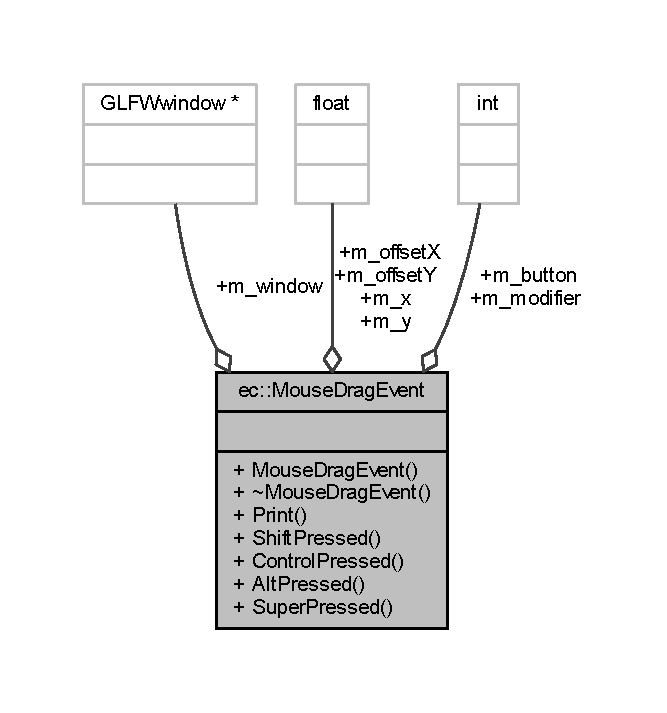
\includegraphics[width=320pt]{structec_1_1_mouse_drag_event__coll__graph}
\end{center}
\end{figure}
\subsection*{Public Member Functions}
\begin{DoxyCompactItemize}
\item 
\mbox{\hyperlink{structec_1_1_mouse_drag_event_a209ef2aaeea4f5fdda4de8f3002798a4}{Mouse\+Drag\+Event}} (G\+L\+F\+Wwindow $\ast$window, const float offsetX, const float offsetY, const float x, const float y, const int button, const int modifier)
\item 
\mbox{\hyperlink{structec_1_1_mouse_drag_event_a589e0ce60c9f229c64e64f4e7b550a80}{$\sim$\+Mouse\+Drag\+Event}} ()
\item 
void \mbox{\hyperlink{structec_1_1_mouse_drag_event_a08827eeaf27a6e24519c1848970fff74}{Print}} () const
\item 
bool \mbox{\hyperlink{structec_1_1_mouse_drag_event_a454cd7a95032be021c77def4a88b9b28}{Shift\+Pressed}} () const
\item 
bool \mbox{\hyperlink{structec_1_1_mouse_drag_event_a3d4f820f2b23c6e0e698472a98fdcdd2}{Control\+Pressed}} () const
\item 
bool \mbox{\hyperlink{structec_1_1_mouse_drag_event_a4d6ef24ef99a3328064f3a46e1e2d48e}{Alt\+Pressed}} () const
\item 
bool \mbox{\hyperlink{structec_1_1_mouse_drag_event_a6399d1f7a18e1d3a754260b5cc15e286}{Super\+Pressed}} () const
\end{DoxyCompactItemize}
\subsection*{Public Attributes}
\begin{DoxyCompactItemize}
\item 
G\+L\+F\+Wwindow $\ast$ \mbox{\hyperlink{structec_1_1_mouse_drag_event_a98e4d2a8236829d2e156eda4a09655bf}{m\+\_\+window}}
\item 
float \mbox{\hyperlink{structec_1_1_mouse_drag_event_a4ebf4f701f677620bc1f76232ca1c9a5}{m\+\_\+x}}
\item 
float \mbox{\hyperlink{structec_1_1_mouse_drag_event_ae66c5f3b087578bfcef4ff1215b50be7}{m\+\_\+y}}
\item 
float \mbox{\hyperlink{structec_1_1_mouse_drag_event_afb2e5e98e6c0014b311d1b4aec103638}{m\+\_\+offsetX}}
\item 
float \mbox{\hyperlink{structec_1_1_mouse_drag_event_a9019720292c490f1a09ecda32f89ae6e}{m\+\_\+offsetY}}
\item 
int \mbox{\hyperlink{structec_1_1_mouse_drag_event_a10244c9d449dd4343281526350e1993f}{m\+\_\+button}}
\item 
int \mbox{\hyperlink{structec_1_1_mouse_drag_event_a9434738e62de520a280e4776232ce1a1}{m\+\_\+modifier}}
\end{DoxyCompactItemize}


\subsection{Constructor \& Destructor Documentation}
\mbox{\Hypertarget{structec_1_1_mouse_drag_event_a209ef2aaeea4f5fdda4de8f3002798a4}\label{structec_1_1_mouse_drag_event_a209ef2aaeea4f5fdda4de8f3002798a4}} 
\index{ec\+::\+Mouse\+Drag\+Event@{ec\+::\+Mouse\+Drag\+Event}!Mouse\+Drag\+Event@{Mouse\+Drag\+Event}}
\index{Mouse\+Drag\+Event@{Mouse\+Drag\+Event}!ec\+::\+Mouse\+Drag\+Event@{ec\+::\+Mouse\+Drag\+Event}}
\subsubsection{\texorpdfstring{Mouse\+Drag\+Event()}{MouseDragEvent()}}
{\footnotesize\ttfamily ec\+::\+Mouse\+Drag\+Event\+::\+Mouse\+Drag\+Event (\begin{DoxyParamCaption}\item[{G\+L\+F\+Wwindow $\ast$}]{window,  }\item[{const float}]{offsetX,  }\item[{const float}]{offsetY,  }\item[{const float}]{x,  }\item[{const float}]{y,  }\item[{const int}]{button,  }\item[{const int}]{modifier }\end{DoxyParamCaption})}

\mbox{\Hypertarget{structec_1_1_mouse_drag_event_a589e0ce60c9f229c64e64f4e7b550a80}\label{structec_1_1_mouse_drag_event_a589e0ce60c9f229c64e64f4e7b550a80}} 
\index{ec\+::\+Mouse\+Drag\+Event@{ec\+::\+Mouse\+Drag\+Event}!````~Mouse\+Drag\+Event@{$\sim$\+Mouse\+Drag\+Event}}
\index{````~Mouse\+Drag\+Event@{$\sim$\+Mouse\+Drag\+Event}!ec\+::\+Mouse\+Drag\+Event@{ec\+::\+Mouse\+Drag\+Event}}
\subsubsection{\texorpdfstring{$\sim$\+Mouse\+Drag\+Event()}{~MouseDragEvent()}}
{\footnotesize\ttfamily ec\+::\+Mouse\+Drag\+Event\+::$\sim$\+Mouse\+Drag\+Event (\begin{DoxyParamCaption}{ }\end{DoxyParamCaption})}



\subsection{Member Function Documentation}
\mbox{\Hypertarget{structec_1_1_mouse_drag_event_a4d6ef24ef99a3328064f3a46e1e2d48e}\label{structec_1_1_mouse_drag_event_a4d6ef24ef99a3328064f3a46e1e2d48e}} 
\index{ec\+::\+Mouse\+Drag\+Event@{ec\+::\+Mouse\+Drag\+Event}!Alt\+Pressed@{Alt\+Pressed}}
\index{Alt\+Pressed@{Alt\+Pressed}!ec\+::\+Mouse\+Drag\+Event@{ec\+::\+Mouse\+Drag\+Event}}
\subsubsection{\texorpdfstring{Alt\+Pressed()}{AltPressed()}}
{\footnotesize\ttfamily bool ec\+::\+Mouse\+Drag\+Event\+::\+Alt\+Pressed (\begin{DoxyParamCaption}{ }\end{DoxyParamCaption}) const}

\mbox{\Hypertarget{structec_1_1_mouse_drag_event_a3d4f820f2b23c6e0e698472a98fdcdd2}\label{structec_1_1_mouse_drag_event_a3d4f820f2b23c6e0e698472a98fdcdd2}} 
\index{ec\+::\+Mouse\+Drag\+Event@{ec\+::\+Mouse\+Drag\+Event}!Control\+Pressed@{Control\+Pressed}}
\index{Control\+Pressed@{Control\+Pressed}!ec\+::\+Mouse\+Drag\+Event@{ec\+::\+Mouse\+Drag\+Event}}
\subsubsection{\texorpdfstring{Control\+Pressed()}{ControlPressed()}}
{\footnotesize\ttfamily bool ec\+::\+Mouse\+Drag\+Event\+::\+Control\+Pressed (\begin{DoxyParamCaption}{ }\end{DoxyParamCaption}) const}

\mbox{\Hypertarget{structec_1_1_mouse_drag_event_a08827eeaf27a6e24519c1848970fff74}\label{structec_1_1_mouse_drag_event_a08827eeaf27a6e24519c1848970fff74}} 
\index{ec\+::\+Mouse\+Drag\+Event@{ec\+::\+Mouse\+Drag\+Event}!Print@{Print}}
\index{Print@{Print}!ec\+::\+Mouse\+Drag\+Event@{ec\+::\+Mouse\+Drag\+Event}}
\subsubsection{\texorpdfstring{Print()}{Print()}}
{\footnotesize\ttfamily void ec\+::\+Mouse\+Drag\+Event\+::\+Print (\begin{DoxyParamCaption}{ }\end{DoxyParamCaption}) const}

\mbox{\Hypertarget{structec_1_1_mouse_drag_event_a454cd7a95032be021c77def4a88b9b28}\label{structec_1_1_mouse_drag_event_a454cd7a95032be021c77def4a88b9b28}} 
\index{ec\+::\+Mouse\+Drag\+Event@{ec\+::\+Mouse\+Drag\+Event}!Shift\+Pressed@{Shift\+Pressed}}
\index{Shift\+Pressed@{Shift\+Pressed}!ec\+::\+Mouse\+Drag\+Event@{ec\+::\+Mouse\+Drag\+Event}}
\subsubsection{\texorpdfstring{Shift\+Pressed()}{ShiftPressed()}}
{\footnotesize\ttfamily bool ec\+::\+Mouse\+Drag\+Event\+::\+Shift\+Pressed (\begin{DoxyParamCaption}{ }\end{DoxyParamCaption}) const}

\mbox{\Hypertarget{structec_1_1_mouse_drag_event_a6399d1f7a18e1d3a754260b5cc15e286}\label{structec_1_1_mouse_drag_event_a6399d1f7a18e1d3a754260b5cc15e286}} 
\index{ec\+::\+Mouse\+Drag\+Event@{ec\+::\+Mouse\+Drag\+Event}!Super\+Pressed@{Super\+Pressed}}
\index{Super\+Pressed@{Super\+Pressed}!ec\+::\+Mouse\+Drag\+Event@{ec\+::\+Mouse\+Drag\+Event}}
\subsubsection{\texorpdfstring{Super\+Pressed()}{SuperPressed()}}
{\footnotesize\ttfamily bool ec\+::\+Mouse\+Drag\+Event\+::\+Super\+Pressed (\begin{DoxyParamCaption}{ }\end{DoxyParamCaption}) const}



\subsection{Member Data Documentation}
\mbox{\Hypertarget{structec_1_1_mouse_drag_event_a10244c9d449dd4343281526350e1993f}\label{structec_1_1_mouse_drag_event_a10244c9d449dd4343281526350e1993f}} 
\index{ec\+::\+Mouse\+Drag\+Event@{ec\+::\+Mouse\+Drag\+Event}!m\+\_\+button@{m\+\_\+button}}
\index{m\+\_\+button@{m\+\_\+button}!ec\+::\+Mouse\+Drag\+Event@{ec\+::\+Mouse\+Drag\+Event}}
\subsubsection{\texorpdfstring{m\+\_\+button}{m\_button}}
{\footnotesize\ttfamily int ec\+::\+Mouse\+Drag\+Event\+::m\+\_\+button}

\mbox{\Hypertarget{structec_1_1_mouse_drag_event_a9434738e62de520a280e4776232ce1a1}\label{structec_1_1_mouse_drag_event_a9434738e62de520a280e4776232ce1a1}} 
\index{ec\+::\+Mouse\+Drag\+Event@{ec\+::\+Mouse\+Drag\+Event}!m\+\_\+modifier@{m\+\_\+modifier}}
\index{m\+\_\+modifier@{m\+\_\+modifier}!ec\+::\+Mouse\+Drag\+Event@{ec\+::\+Mouse\+Drag\+Event}}
\subsubsection{\texorpdfstring{m\+\_\+modifier}{m\_modifier}}
{\footnotesize\ttfamily int ec\+::\+Mouse\+Drag\+Event\+::m\+\_\+modifier}

\mbox{\Hypertarget{structec_1_1_mouse_drag_event_afb2e5e98e6c0014b311d1b4aec103638}\label{structec_1_1_mouse_drag_event_afb2e5e98e6c0014b311d1b4aec103638}} 
\index{ec\+::\+Mouse\+Drag\+Event@{ec\+::\+Mouse\+Drag\+Event}!m\+\_\+offsetX@{m\+\_\+offsetX}}
\index{m\+\_\+offsetX@{m\+\_\+offsetX}!ec\+::\+Mouse\+Drag\+Event@{ec\+::\+Mouse\+Drag\+Event}}
\subsubsection{\texorpdfstring{m\+\_\+offsetX}{m\_offsetX}}
{\footnotesize\ttfamily float ec\+::\+Mouse\+Drag\+Event\+::m\+\_\+offsetX}

\mbox{\Hypertarget{structec_1_1_mouse_drag_event_a9019720292c490f1a09ecda32f89ae6e}\label{structec_1_1_mouse_drag_event_a9019720292c490f1a09ecda32f89ae6e}} 
\index{ec\+::\+Mouse\+Drag\+Event@{ec\+::\+Mouse\+Drag\+Event}!m\+\_\+offsetY@{m\+\_\+offsetY}}
\index{m\+\_\+offsetY@{m\+\_\+offsetY}!ec\+::\+Mouse\+Drag\+Event@{ec\+::\+Mouse\+Drag\+Event}}
\subsubsection{\texorpdfstring{m\+\_\+offsetY}{m\_offsetY}}
{\footnotesize\ttfamily float ec\+::\+Mouse\+Drag\+Event\+::m\+\_\+offsetY}

\mbox{\Hypertarget{structec_1_1_mouse_drag_event_a98e4d2a8236829d2e156eda4a09655bf}\label{structec_1_1_mouse_drag_event_a98e4d2a8236829d2e156eda4a09655bf}} 
\index{ec\+::\+Mouse\+Drag\+Event@{ec\+::\+Mouse\+Drag\+Event}!m\+\_\+window@{m\+\_\+window}}
\index{m\+\_\+window@{m\+\_\+window}!ec\+::\+Mouse\+Drag\+Event@{ec\+::\+Mouse\+Drag\+Event}}
\subsubsection{\texorpdfstring{m\+\_\+window}{m\_window}}
{\footnotesize\ttfamily G\+L\+F\+Wwindow$\ast$ ec\+::\+Mouse\+Drag\+Event\+::m\+\_\+window}

\mbox{\Hypertarget{structec_1_1_mouse_drag_event_a4ebf4f701f677620bc1f76232ca1c9a5}\label{structec_1_1_mouse_drag_event_a4ebf4f701f677620bc1f76232ca1c9a5}} 
\index{ec\+::\+Mouse\+Drag\+Event@{ec\+::\+Mouse\+Drag\+Event}!m\+\_\+x@{m\+\_\+x}}
\index{m\+\_\+x@{m\+\_\+x}!ec\+::\+Mouse\+Drag\+Event@{ec\+::\+Mouse\+Drag\+Event}}
\subsubsection{\texorpdfstring{m\+\_\+x}{m\_x}}
{\footnotesize\ttfamily float ec\+::\+Mouse\+Drag\+Event\+::m\+\_\+x}

\mbox{\Hypertarget{structec_1_1_mouse_drag_event_ae66c5f3b087578bfcef4ff1215b50be7}\label{structec_1_1_mouse_drag_event_ae66c5f3b087578bfcef4ff1215b50be7}} 
\index{ec\+::\+Mouse\+Drag\+Event@{ec\+::\+Mouse\+Drag\+Event}!m\+\_\+y@{m\+\_\+y}}
\index{m\+\_\+y@{m\+\_\+y}!ec\+::\+Mouse\+Drag\+Event@{ec\+::\+Mouse\+Drag\+Event}}
\subsubsection{\texorpdfstring{m\+\_\+y}{m\_y}}
{\footnotesize\ttfamily float ec\+::\+Mouse\+Drag\+Event\+::m\+\_\+y}



The documentation for this struct was generated from the following files\+:\begin{DoxyCompactItemize}
\item 
D\+:/\+Library/\+Documents/\+Job/\+Forschungsmaster/\+Projekte/\+Eye\+Candy3\+D/\+Eye\+Candy3\+D/include/\+E\+C3\+D/\+Core/\mbox{\hyperlink{_input_event_8h}{Input\+Event.\+h}}\item 
D\+:/\+Library/\+Documents/\+Job/\+Forschungsmaster/\+Projekte/\+Eye\+Candy3\+D/\+Eye\+Candy3\+D/src/\+Core/\mbox{\hyperlink{_input_event_8cpp}{Input\+Event.\+cpp}}\end{DoxyCompactItemize}

\hypertarget{structec_1_1_mouse_enter_event}{}\section{ec\+:\+:Mouse\+Enter\+Event Struct Reference}
\label{structec_1_1_mouse_enter_event}\index{ec\+::\+Mouse\+Enter\+Event@{ec\+::\+Mouse\+Enter\+Event}}


{\ttfamily \#include $<$Input\+Event.\+h$>$}



Collaboration diagram for ec\+:\+:Mouse\+Enter\+Event\+:\nopagebreak
\begin{figure}[H]
\begin{center}
\leavevmode
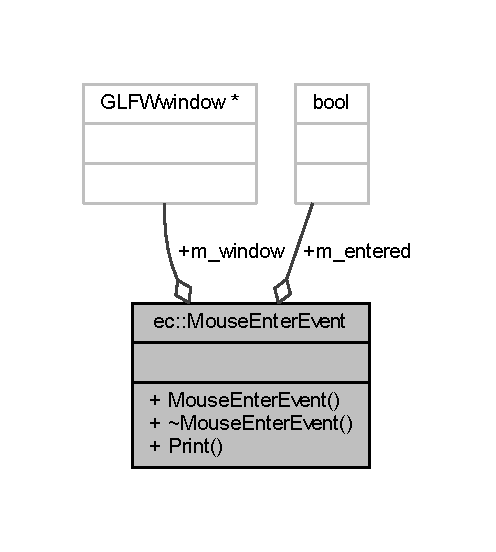
\includegraphics[width=238pt]{structec_1_1_mouse_enter_event__coll__graph}
\end{center}
\end{figure}
\subsection*{Public Member Functions}
\begin{DoxyCompactItemize}
\item 
\mbox{\hyperlink{structec_1_1_mouse_enter_event_a8683590d2b99dbb3bf3db3cd50951797}{Mouse\+Enter\+Event}} (G\+L\+F\+Wwindow $\ast$window, const bool entered)
\item 
\mbox{\hyperlink{structec_1_1_mouse_enter_event_accbd4fca68e8e582493fa3d636b9d293}{$\sim$\+Mouse\+Enter\+Event}} ()
\item 
void \mbox{\hyperlink{structec_1_1_mouse_enter_event_a341f8c9ee2ee87e4f8c74af90c2fe29d}{Print}} () const
\end{DoxyCompactItemize}
\subsection*{Public Attributes}
\begin{DoxyCompactItemize}
\item 
G\+L\+F\+Wwindow $\ast$ \mbox{\hyperlink{structec_1_1_mouse_enter_event_affdb33db16df7493f83e19cd70cfea3c}{m\+\_\+window}}
\item 
bool \mbox{\hyperlink{structec_1_1_mouse_enter_event_ae778f98aa805ff1ce3ba6872177e3fd1}{m\+\_\+entered}}
\end{DoxyCompactItemize}


\subsection{Constructor \& Destructor Documentation}
\mbox{\Hypertarget{structec_1_1_mouse_enter_event_a8683590d2b99dbb3bf3db3cd50951797}\label{structec_1_1_mouse_enter_event_a8683590d2b99dbb3bf3db3cd50951797}} 
\index{ec\+::\+Mouse\+Enter\+Event@{ec\+::\+Mouse\+Enter\+Event}!Mouse\+Enter\+Event@{Mouse\+Enter\+Event}}
\index{Mouse\+Enter\+Event@{Mouse\+Enter\+Event}!ec\+::\+Mouse\+Enter\+Event@{ec\+::\+Mouse\+Enter\+Event}}
\subsubsection{\texorpdfstring{Mouse\+Enter\+Event()}{MouseEnterEvent()}}
{\footnotesize\ttfamily ec\+::\+Mouse\+Enter\+Event\+::\+Mouse\+Enter\+Event (\begin{DoxyParamCaption}\item[{G\+L\+F\+Wwindow $\ast$}]{window,  }\item[{const bool}]{entered }\end{DoxyParamCaption})}

\mbox{\Hypertarget{structec_1_1_mouse_enter_event_accbd4fca68e8e582493fa3d636b9d293}\label{structec_1_1_mouse_enter_event_accbd4fca68e8e582493fa3d636b9d293}} 
\index{ec\+::\+Mouse\+Enter\+Event@{ec\+::\+Mouse\+Enter\+Event}!````~Mouse\+Enter\+Event@{$\sim$\+Mouse\+Enter\+Event}}
\index{````~Mouse\+Enter\+Event@{$\sim$\+Mouse\+Enter\+Event}!ec\+::\+Mouse\+Enter\+Event@{ec\+::\+Mouse\+Enter\+Event}}
\subsubsection{\texorpdfstring{$\sim$\+Mouse\+Enter\+Event()}{~MouseEnterEvent()}}
{\footnotesize\ttfamily ec\+::\+Mouse\+Enter\+Event\+::$\sim$\+Mouse\+Enter\+Event (\begin{DoxyParamCaption}{ }\end{DoxyParamCaption})}



\subsection{Member Function Documentation}
\mbox{\Hypertarget{structec_1_1_mouse_enter_event_a341f8c9ee2ee87e4f8c74af90c2fe29d}\label{structec_1_1_mouse_enter_event_a341f8c9ee2ee87e4f8c74af90c2fe29d}} 
\index{ec\+::\+Mouse\+Enter\+Event@{ec\+::\+Mouse\+Enter\+Event}!Print@{Print}}
\index{Print@{Print}!ec\+::\+Mouse\+Enter\+Event@{ec\+::\+Mouse\+Enter\+Event}}
\subsubsection{\texorpdfstring{Print()}{Print()}}
{\footnotesize\ttfamily void ec\+::\+Mouse\+Enter\+Event\+::\+Print (\begin{DoxyParamCaption}{ }\end{DoxyParamCaption}) const}



\subsection{Member Data Documentation}
\mbox{\Hypertarget{structec_1_1_mouse_enter_event_ae778f98aa805ff1ce3ba6872177e3fd1}\label{structec_1_1_mouse_enter_event_ae778f98aa805ff1ce3ba6872177e3fd1}} 
\index{ec\+::\+Mouse\+Enter\+Event@{ec\+::\+Mouse\+Enter\+Event}!m\+\_\+entered@{m\+\_\+entered}}
\index{m\+\_\+entered@{m\+\_\+entered}!ec\+::\+Mouse\+Enter\+Event@{ec\+::\+Mouse\+Enter\+Event}}
\subsubsection{\texorpdfstring{m\+\_\+entered}{m\_entered}}
{\footnotesize\ttfamily bool ec\+::\+Mouse\+Enter\+Event\+::m\+\_\+entered}

\mbox{\Hypertarget{structec_1_1_mouse_enter_event_affdb33db16df7493f83e19cd70cfea3c}\label{structec_1_1_mouse_enter_event_affdb33db16df7493f83e19cd70cfea3c}} 
\index{ec\+::\+Mouse\+Enter\+Event@{ec\+::\+Mouse\+Enter\+Event}!m\+\_\+window@{m\+\_\+window}}
\index{m\+\_\+window@{m\+\_\+window}!ec\+::\+Mouse\+Enter\+Event@{ec\+::\+Mouse\+Enter\+Event}}
\subsubsection{\texorpdfstring{m\+\_\+window}{m\_window}}
{\footnotesize\ttfamily G\+L\+F\+Wwindow$\ast$ ec\+::\+Mouse\+Enter\+Event\+::m\+\_\+window}



The documentation for this struct was generated from the following files\+:\begin{DoxyCompactItemize}
\item 
D\+:/\+Library/\+Documents/\+Job/\+Forschungsmaster/\+Projekte/\+Eye\+Candy3\+D/\+Eye\+Candy3\+D/include/\+E\+C3\+D/\+Core/\mbox{\hyperlink{_input_event_8h}{Input\+Event.\+h}}\item 
D\+:/\+Library/\+Documents/\+Job/\+Forschungsmaster/\+Projekte/\+Eye\+Candy3\+D/\+Eye\+Candy3\+D/src/\+Core/\mbox{\hyperlink{_input_event_8cpp}{Input\+Event.\+cpp}}\end{DoxyCompactItemize}

\hypertarget{structec_1_1_mouse_move_event}{}\section{ec\+:\+:Mouse\+Move\+Event Struct Reference}
\label{structec_1_1_mouse_move_event}\index{ec\+::\+Mouse\+Move\+Event@{ec\+::\+Mouse\+Move\+Event}}


{\ttfamily \#include $<$Input\+Event.\+h$>$}



Collaboration diagram for ec\+:\+:Mouse\+Move\+Event\+:\nopagebreak
\begin{figure}[H]
\begin{center}
\leavevmode
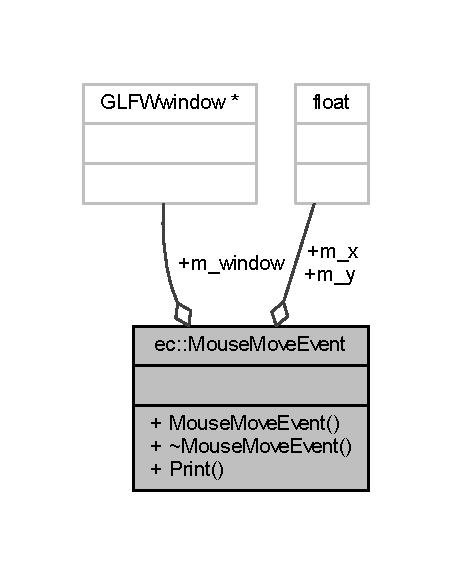
\includegraphics[width=217pt]{structec_1_1_mouse_move_event__coll__graph}
\end{center}
\end{figure}
\subsection*{Public Member Functions}
\begin{DoxyCompactItemize}
\item 
\mbox{\hyperlink{structec_1_1_mouse_move_event_a3783a260f9b525df43a628cc2dff7611}{Mouse\+Move\+Event}} (G\+L\+F\+Wwindow $\ast$window, const float x, const float y)
\item 
\mbox{\hyperlink{structec_1_1_mouse_move_event_a9839ac53047ea0bcfd23010b66c9cef5}{$\sim$\+Mouse\+Move\+Event}} ()
\item 
void \mbox{\hyperlink{structec_1_1_mouse_move_event_ab45ddd0c88e0c5a669a99d755fac3e99}{Print}} () const
\end{DoxyCompactItemize}
\subsection*{Public Attributes}
\begin{DoxyCompactItemize}
\item 
G\+L\+F\+Wwindow $\ast$ \mbox{\hyperlink{structec_1_1_mouse_move_event_ac1205c64a8f812566eeee2c83a4df824}{m\+\_\+window}}
\item 
float \mbox{\hyperlink{structec_1_1_mouse_move_event_a2e6f479609b2919db2623111e240284e}{m\+\_\+x}}
\item 
float \mbox{\hyperlink{structec_1_1_mouse_move_event_a559559f7d2ae5a689963f71f28ad2409}{m\+\_\+y}}
\end{DoxyCompactItemize}


\subsection{Constructor \& Destructor Documentation}
\mbox{\Hypertarget{structec_1_1_mouse_move_event_a3783a260f9b525df43a628cc2dff7611}\label{structec_1_1_mouse_move_event_a3783a260f9b525df43a628cc2dff7611}} 
\index{ec\+::\+Mouse\+Move\+Event@{ec\+::\+Mouse\+Move\+Event}!Mouse\+Move\+Event@{Mouse\+Move\+Event}}
\index{Mouse\+Move\+Event@{Mouse\+Move\+Event}!ec\+::\+Mouse\+Move\+Event@{ec\+::\+Mouse\+Move\+Event}}
\subsubsection{\texorpdfstring{Mouse\+Move\+Event()}{MouseMoveEvent()}}
{\footnotesize\ttfamily ec\+::\+Mouse\+Move\+Event\+::\+Mouse\+Move\+Event (\begin{DoxyParamCaption}\item[{G\+L\+F\+Wwindow $\ast$}]{window,  }\item[{const float}]{x,  }\item[{const float}]{y }\end{DoxyParamCaption})}

\mbox{\Hypertarget{structec_1_1_mouse_move_event_a9839ac53047ea0bcfd23010b66c9cef5}\label{structec_1_1_mouse_move_event_a9839ac53047ea0bcfd23010b66c9cef5}} 
\index{ec\+::\+Mouse\+Move\+Event@{ec\+::\+Mouse\+Move\+Event}!````~Mouse\+Move\+Event@{$\sim$\+Mouse\+Move\+Event}}
\index{````~Mouse\+Move\+Event@{$\sim$\+Mouse\+Move\+Event}!ec\+::\+Mouse\+Move\+Event@{ec\+::\+Mouse\+Move\+Event}}
\subsubsection{\texorpdfstring{$\sim$\+Mouse\+Move\+Event()}{~MouseMoveEvent()}}
{\footnotesize\ttfamily ec\+::\+Mouse\+Move\+Event\+::$\sim$\+Mouse\+Move\+Event (\begin{DoxyParamCaption}{ }\end{DoxyParamCaption})}



\subsection{Member Function Documentation}
\mbox{\Hypertarget{structec_1_1_mouse_move_event_ab45ddd0c88e0c5a669a99d755fac3e99}\label{structec_1_1_mouse_move_event_ab45ddd0c88e0c5a669a99d755fac3e99}} 
\index{ec\+::\+Mouse\+Move\+Event@{ec\+::\+Mouse\+Move\+Event}!Print@{Print}}
\index{Print@{Print}!ec\+::\+Mouse\+Move\+Event@{ec\+::\+Mouse\+Move\+Event}}
\subsubsection{\texorpdfstring{Print()}{Print()}}
{\footnotesize\ttfamily void ec\+::\+Mouse\+Move\+Event\+::\+Print (\begin{DoxyParamCaption}{ }\end{DoxyParamCaption}) const}



\subsection{Member Data Documentation}
\mbox{\Hypertarget{structec_1_1_mouse_move_event_ac1205c64a8f812566eeee2c83a4df824}\label{structec_1_1_mouse_move_event_ac1205c64a8f812566eeee2c83a4df824}} 
\index{ec\+::\+Mouse\+Move\+Event@{ec\+::\+Mouse\+Move\+Event}!m\+\_\+window@{m\+\_\+window}}
\index{m\+\_\+window@{m\+\_\+window}!ec\+::\+Mouse\+Move\+Event@{ec\+::\+Mouse\+Move\+Event}}
\subsubsection{\texorpdfstring{m\+\_\+window}{m\_window}}
{\footnotesize\ttfamily G\+L\+F\+Wwindow$\ast$ ec\+::\+Mouse\+Move\+Event\+::m\+\_\+window}

\mbox{\Hypertarget{structec_1_1_mouse_move_event_a2e6f479609b2919db2623111e240284e}\label{structec_1_1_mouse_move_event_a2e6f479609b2919db2623111e240284e}} 
\index{ec\+::\+Mouse\+Move\+Event@{ec\+::\+Mouse\+Move\+Event}!m\+\_\+x@{m\+\_\+x}}
\index{m\+\_\+x@{m\+\_\+x}!ec\+::\+Mouse\+Move\+Event@{ec\+::\+Mouse\+Move\+Event}}
\subsubsection{\texorpdfstring{m\+\_\+x}{m\_x}}
{\footnotesize\ttfamily float ec\+::\+Mouse\+Move\+Event\+::m\+\_\+x}

\mbox{\Hypertarget{structec_1_1_mouse_move_event_a559559f7d2ae5a689963f71f28ad2409}\label{structec_1_1_mouse_move_event_a559559f7d2ae5a689963f71f28ad2409}} 
\index{ec\+::\+Mouse\+Move\+Event@{ec\+::\+Mouse\+Move\+Event}!m\+\_\+y@{m\+\_\+y}}
\index{m\+\_\+y@{m\+\_\+y}!ec\+::\+Mouse\+Move\+Event@{ec\+::\+Mouse\+Move\+Event}}
\subsubsection{\texorpdfstring{m\+\_\+y}{m\_y}}
{\footnotesize\ttfamily float ec\+::\+Mouse\+Move\+Event\+::m\+\_\+y}



The documentation for this struct was generated from the following files\+:\begin{DoxyCompactItemize}
\item 
D\+:/\+Library/\+Documents/\+Job/\+Forschungsmaster/\+Projekte/\+Eye\+Candy3\+D/\+Eye\+Candy3\+D/include/\+E\+C3\+D/\+Core/\mbox{\hyperlink{_input_event_8h}{Input\+Event.\+h}}\item 
D\+:/\+Library/\+Documents/\+Job/\+Forschungsmaster/\+Projekte/\+Eye\+Candy3\+D/\+Eye\+Candy3\+D/src/\+Core/\mbox{\hyperlink{_input_event_8cpp}{Input\+Event.\+cpp}}\end{DoxyCompactItemize}

\hypertarget{structec_1_1_mouse_scroll_event}{}\section{ec\+:\+:Mouse\+Scroll\+Event Struct Reference}
\label{structec_1_1_mouse_scroll_event}\index{ec\+::\+Mouse\+Scroll\+Event@{ec\+::\+Mouse\+Scroll\+Event}}


{\ttfamily \#include $<$Input\+Event.\+h$>$}



Collaboration diagram for ec\+:\+:Mouse\+Scroll\+Event\+:\nopagebreak
\begin{figure}[H]
\begin{center}
\leavevmode
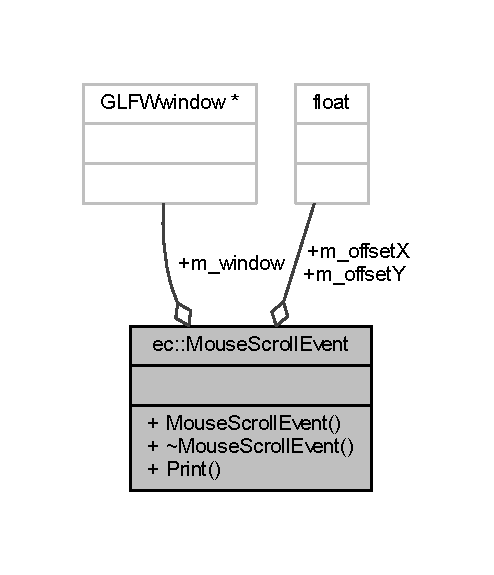
\includegraphics[width=237pt]{structec_1_1_mouse_scroll_event__coll__graph}
\end{center}
\end{figure}
\subsection*{Public Member Functions}
\begin{DoxyCompactItemize}
\item 
\mbox{\hyperlink{structec_1_1_mouse_scroll_event_a3bccf854cfd63d44a49db296fc88b8dd}{Mouse\+Scroll\+Event}} (G\+L\+F\+Wwindow $\ast$window, const float offsetX, const float offsetY)
\item 
\mbox{\hyperlink{structec_1_1_mouse_scroll_event_a253aa9552ed33bc767b64057c0d4a457}{$\sim$\+Mouse\+Scroll\+Event}} ()
\item 
void \mbox{\hyperlink{structec_1_1_mouse_scroll_event_a32d077172f91f04909d469e070e219e6}{Print}} () const
\end{DoxyCompactItemize}
\subsection*{Public Attributes}
\begin{DoxyCompactItemize}
\item 
G\+L\+F\+Wwindow $\ast$ \mbox{\hyperlink{structec_1_1_mouse_scroll_event_a76f795ff6bd0629d496005b8e415552a}{m\+\_\+window}}
\item 
float \mbox{\hyperlink{structec_1_1_mouse_scroll_event_a1925678027669178fcdd37bb3f3c034d}{m\+\_\+offsetX}}
\item 
float \mbox{\hyperlink{structec_1_1_mouse_scroll_event_ac366f5d0fb127838cca2387b7af61524}{m\+\_\+offsetY}}
\end{DoxyCompactItemize}


\subsection{Constructor \& Destructor Documentation}
\mbox{\Hypertarget{structec_1_1_mouse_scroll_event_a3bccf854cfd63d44a49db296fc88b8dd}\label{structec_1_1_mouse_scroll_event_a3bccf854cfd63d44a49db296fc88b8dd}} 
\index{ec\+::\+Mouse\+Scroll\+Event@{ec\+::\+Mouse\+Scroll\+Event}!Mouse\+Scroll\+Event@{Mouse\+Scroll\+Event}}
\index{Mouse\+Scroll\+Event@{Mouse\+Scroll\+Event}!ec\+::\+Mouse\+Scroll\+Event@{ec\+::\+Mouse\+Scroll\+Event}}
\subsubsection{\texorpdfstring{Mouse\+Scroll\+Event()}{MouseScrollEvent()}}
{\footnotesize\ttfamily ec\+::\+Mouse\+Scroll\+Event\+::\+Mouse\+Scroll\+Event (\begin{DoxyParamCaption}\item[{G\+L\+F\+Wwindow $\ast$}]{window,  }\item[{const float}]{offsetX,  }\item[{const float}]{offsetY }\end{DoxyParamCaption})}

\mbox{\Hypertarget{structec_1_1_mouse_scroll_event_a253aa9552ed33bc767b64057c0d4a457}\label{structec_1_1_mouse_scroll_event_a253aa9552ed33bc767b64057c0d4a457}} 
\index{ec\+::\+Mouse\+Scroll\+Event@{ec\+::\+Mouse\+Scroll\+Event}!````~Mouse\+Scroll\+Event@{$\sim$\+Mouse\+Scroll\+Event}}
\index{````~Mouse\+Scroll\+Event@{$\sim$\+Mouse\+Scroll\+Event}!ec\+::\+Mouse\+Scroll\+Event@{ec\+::\+Mouse\+Scroll\+Event}}
\subsubsection{\texorpdfstring{$\sim$\+Mouse\+Scroll\+Event()}{~MouseScrollEvent()}}
{\footnotesize\ttfamily ec\+::\+Mouse\+Scroll\+Event\+::$\sim$\+Mouse\+Scroll\+Event (\begin{DoxyParamCaption}{ }\end{DoxyParamCaption})}



\subsection{Member Function Documentation}
\mbox{\Hypertarget{structec_1_1_mouse_scroll_event_a32d077172f91f04909d469e070e219e6}\label{structec_1_1_mouse_scroll_event_a32d077172f91f04909d469e070e219e6}} 
\index{ec\+::\+Mouse\+Scroll\+Event@{ec\+::\+Mouse\+Scroll\+Event}!Print@{Print}}
\index{Print@{Print}!ec\+::\+Mouse\+Scroll\+Event@{ec\+::\+Mouse\+Scroll\+Event}}
\subsubsection{\texorpdfstring{Print()}{Print()}}
{\footnotesize\ttfamily void ec\+::\+Mouse\+Scroll\+Event\+::\+Print (\begin{DoxyParamCaption}{ }\end{DoxyParamCaption}) const}



\subsection{Member Data Documentation}
\mbox{\Hypertarget{structec_1_1_mouse_scroll_event_a1925678027669178fcdd37bb3f3c034d}\label{structec_1_1_mouse_scroll_event_a1925678027669178fcdd37bb3f3c034d}} 
\index{ec\+::\+Mouse\+Scroll\+Event@{ec\+::\+Mouse\+Scroll\+Event}!m\+\_\+offsetX@{m\+\_\+offsetX}}
\index{m\+\_\+offsetX@{m\+\_\+offsetX}!ec\+::\+Mouse\+Scroll\+Event@{ec\+::\+Mouse\+Scroll\+Event}}
\subsubsection{\texorpdfstring{m\+\_\+offsetX}{m\_offsetX}}
{\footnotesize\ttfamily float ec\+::\+Mouse\+Scroll\+Event\+::m\+\_\+offsetX}

\mbox{\Hypertarget{structec_1_1_mouse_scroll_event_ac366f5d0fb127838cca2387b7af61524}\label{structec_1_1_mouse_scroll_event_ac366f5d0fb127838cca2387b7af61524}} 
\index{ec\+::\+Mouse\+Scroll\+Event@{ec\+::\+Mouse\+Scroll\+Event}!m\+\_\+offsetY@{m\+\_\+offsetY}}
\index{m\+\_\+offsetY@{m\+\_\+offsetY}!ec\+::\+Mouse\+Scroll\+Event@{ec\+::\+Mouse\+Scroll\+Event}}
\subsubsection{\texorpdfstring{m\+\_\+offsetY}{m\_offsetY}}
{\footnotesize\ttfamily float ec\+::\+Mouse\+Scroll\+Event\+::m\+\_\+offsetY}

\mbox{\Hypertarget{structec_1_1_mouse_scroll_event_a76f795ff6bd0629d496005b8e415552a}\label{structec_1_1_mouse_scroll_event_a76f795ff6bd0629d496005b8e415552a}} 
\index{ec\+::\+Mouse\+Scroll\+Event@{ec\+::\+Mouse\+Scroll\+Event}!m\+\_\+window@{m\+\_\+window}}
\index{m\+\_\+window@{m\+\_\+window}!ec\+::\+Mouse\+Scroll\+Event@{ec\+::\+Mouse\+Scroll\+Event}}
\subsubsection{\texorpdfstring{m\+\_\+window}{m\_window}}
{\footnotesize\ttfamily G\+L\+F\+Wwindow$\ast$ ec\+::\+Mouse\+Scroll\+Event\+::m\+\_\+window}



The documentation for this struct was generated from the following files\+:\begin{DoxyCompactItemize}
\item 
D\+:/\+Library/\+Documents/\+Job/\+Forschungsmaster/\+Projekte/\+Eye\+Candy3\+D/\+Eye\+Candy3\+D/include/\+E\+C3\+D/\+Core/\mbox{\hyperlink{_input_event_8h}{Input\+Event.\+h}}\item 
D\+:/\+Library/\+Documents/\+Job/\+Forschungsmaster/\+Projekte/\+Eye\+Candy3\+D/\+Eye\+Candy3\+D/src/\+Core/\mbox{\hyperlink{_input_event_8cpp}{Input\+Event.\+cpp}}\end{DoxyCompactItemize}

\hypertarget{classec_1_1_node}{}\section{ec\+:\+:Node Class Reference}
\label{classec_1_1_node}\index{ec\+::\+Node@{ec\+::\+Node}}


{\ttfamily \#include $<$Node.\+h$>$}



Collaboration diagram for ec\+:\+:Node\+:
\nopagebreak
\begin{figure}[H]
\begin{center}
\leavevmode
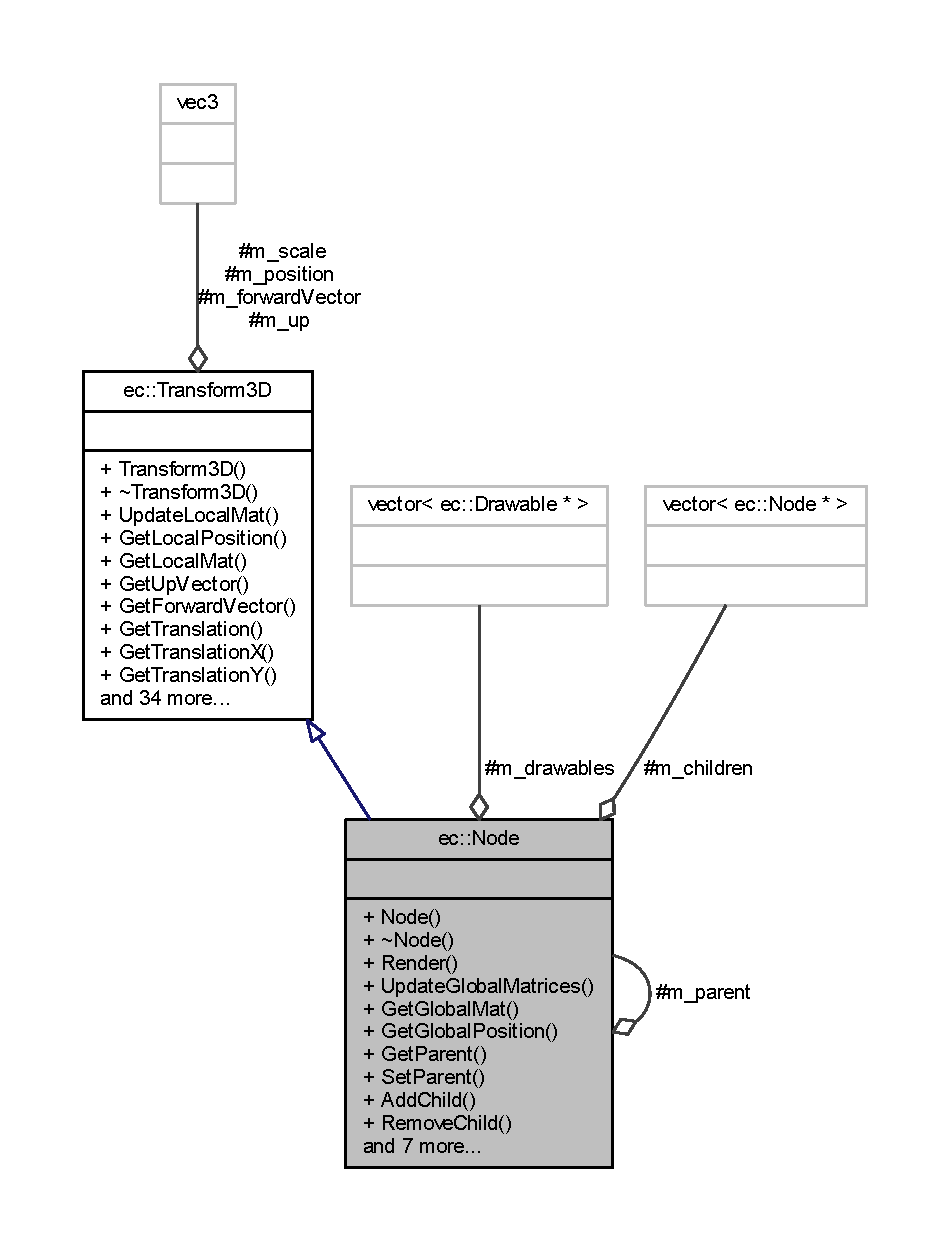
\includegraphics[width=350pt]{classec_1_1_node__coll__graph}
\end{center}
\end{figure}
\subsection*{Public Member Functions}
\begin{DoxyCompactItemize}
\item 
\mbox{\hyperlink{classec_1_1_node_a99fb4715fbc3f193ad5ed88dff15cd0e}{Node}} (\mbox{\hyperlink{classec_1_1_node}{Node}} $\ast$parent)
\item 
virtual \mbox{\hyperlink{classec_1_1_node_a6b2dfa6d2490ec46a5d15a326780889b}{$\sim$\+Node}} ()
\item 
virtual void \mbox{\hyperlink{classec_1_1_node_ac606be4f6d5a899a0b9679b6767ff109}{Render}} (\mbox{\hyperlink{classec_1_1_scene_renderer}{Scene\+Renderer}} \&renderer)
\item 
void \mbox{\hyperlink{classec_1_1_node_ac9970ec0ec03e130da59d0d5376a9855}{Update\+Global\+Matrices}} (const glm\+::mat4 \&m\+\_\+parent\+Mat)
\item 
const glm\+::mat4 \& \mbox{\hyperlink{classec_1_1_node_aafbc9c31eb710b1ac22834792e039435}{Get\+Global\+Mat}} () const
\item 
\mbox{\hyperlink{classec_1_1_node}{Node}} $\ast$ \mbox{\hyperlink{classec_1_1_node_a88919835b03a7055f4c1c50c68b83fac}{Get\+Parent}} ()
\item 
void \mbox{\hyperlink{classec_1_1_node_abda1732f28b0f81df2028d889eb73bdf}{Set\+Parent}} (\mbox{\hyperlink{classec_1_1_node}{Node}} $\ast$parent)
\item 
void \mbox{\hyperlink{classec_1_1_node_a769243d9432b14a0c4362c98f4c89a73}{Add\+Child}} (\mbox{\hyperlink{classec_1_1_node}{Node}} $\ast$child)
\item 
bool \mbox{\hyperlink{classec_1_1_node_a65f938c730afc4f5b4fcceb64ac84416}{Remove\+Child}} (\mbox{\hyperlink{classec_1_1_node}{Node}} $\ast$child)
\item 
void \mbox{\hyperlink{classec_1_1_node_ae91a96819729bc06c17870fa8cca2129}{Remove\+Children}} ()
\item 
unsigned int \mbox{\hyperlink{classec_1_1_node_afc08689badadadcbbca919858994d30b}{Get\+Children\+Count}} () const
\item 
bool \mbox{\hyperlink{classec_1_1_node_add6f4b234aebaeb7d1e76d42234b9831}{Has\+Children}} () const
\item 
virtual const std\+::vector$<$ \mbox{\hyperlink{classec_1_1_drawable}{Drawable}} $\ast$ $>$ \& \mbox{\hyperlink{classec_1_1_node_ab1cd50204e1b38c9c1b31e46d13ea915}{Get\+Drawables}} () const
\item 
void \mbox{\hyperlink{classec_1_1_node_aee80ae03faf344743ab38944ce3ced5f}{Add\+Drawable}} (\mbox{\hyperlink{classec_1_1_drawable}{Drawable}} $\ast$\mbox{\hyperlink{namespaceec_ae4420ccd0f79418a5ce075e43909289fac571a3227368b17e0ecc38a2a417e201}{drawable}})
\item 
void \mbox{\hyperlink{classec_1_1_node_acd641d3927ae368628ac90d5d79597d9}{Remove\+Drawable}} (\mbox{\hyperlink{classec_1_1_drawable}{Drawable}} $\ast$\mbox{\hyperlink{namespaceec_ae4420ccd0f79418a5ce075e43909289fac571a3227368b17e0ecc38a2a417e201}{drawable}})
\item 
void \mbox{\hyperlink{classec_1_1_node_ad874f229d3602ac6f0d0f0ce502a1fbc}{Remove\+Drawables}} ()
\item 
const glm\+::mat4 \& \mbox{\hyperlink{classec_1_1_node_a166d54a9128b6f4d552cf83d8f10856c}{Get\+Local\+Matrix}} () const
\item 
const glm\+::mat4 \& \mbox{\hyperlink{classec_1_1_node_a65650fa6bb55597cc2436949e95321ca}{Get\+Global\+Matrix}} () const
\item 
void \mbox{\hyperlink{classec_1_1_node_a6fa8ebdc20482b2bceb518b1e14b44de}{Translate}} (const glm\+::vec3 \&val)
\item 
void \mbox{\hyperlink{classec_1_1_node_a04817a276d8ba5432d6a42f4403520ef}{TranslateX}} (float x)
\item 
void \mbox{\hyperlink{classec_1_1_node_a823a4ed88acaf530b29901bb8c50e920}{TranslateY}} (float y)
\item 
void \mbox{\hyperlink{classec_1_1_node_a4f3622e18ba67afc383d69f31c073b8e}{TranslateZ}} (float z)
\item 
void \mbox{\hyperlink{classec_1_1_node_a4948bc000406051044e4bc9fa4c3f799}{Set\+Translation}} (const glm\+::vec3 \&val)
\item 
glm\+::vec3 \mbox{\hyperlink{classec_1_1_node_ae29fe5673f7007449d2efa0e599ac0db}{Get\+Translation}} () const
\item 
void \mbox{\hyperlink{classec_1_1_node_a131b4280ff9eba0a9cdf1280e2974fcc}{Rotate}} (const float angle, const glm\+::vec3 \&axis)
\item 
void \mbox{\hyperlink{classec_1_1_node_a4b00f16b05542f0abfcc7eafbad50319}{Set\+Orientation}} (const glm\+::vec3 \&orientation)
\item 
glm\+::vec3 \mbox{\hyperlink{classec_1_1_node_a841071e180e27ad6ced9878aa284c933}{Set\+Orientation}} () const
\item 
void \mbox{\hyperlink{classec_1_1_node_acd826d1dcd58f5588b8ea75068ddff67}{Scale}} (const glm\+::vec3 \&val)
\item 
void \mbox{\hyperlink{classec_1_1_node_a13c6ef1c96edf0027f66be0c7457bd83}{Set\+Scale}} (const glm\+::vec3 \&val)
\item 
glm\+::vec3 \mbox{\hyperlink{classec_1_1_node_ac77ed7b5dd0920f72484a36b665f8883}{Get\+Scale}} () const
\end{DoxyCompactItemize}
\subsection*{Protected Attributes}
\begin{DoxyCompactItemize}
\item 
\mbox{\hyperlink{classec_1_1_node}{Node}} $\ast$ \mbox{\hyperlink{classec_1_1_node_a9f5373bd3ba5bfed53894223adcfe791}{m\+\_\+parent}}
\item 
std\+::vector$<$ \mbox{\hyperlink{classec_1_1_node}{Node}} $\ast$ $>$ \mbox{\hyperlink{classec_1_1_node_a648e1758013c7fc5899cbff2f8fe41fa}{m\+\_\+children}}
\item 
std\+::vector$<$ \mbox{\hyperlink{classec_1_1_drawable}{Drawable}} $\ast$ $>$ \mbox{\hyperlink{classec_1_1_node_aa9f624971a4906674148117ba4442c01}{m\+\_\+drawables}}
\item 
glm\+::mat4 \mbox{\hyperlink{classec_1_1_node_af8842c1cf2027d0890f8529c2fafaf2d}{m\+\_\+local\+Mat}}
\end{DoxyCompactItemize}


\subsection{Constructor \& Destructor Documentation}
\mbox{\Hypertarget{classec_1_1_node_a99fb4715fbc3f193ad5ed88dff15cd0e}\label{classec_1_1_node_a99fb4715fbc3f193ad5ed88dff15cd0e}} 
\index{ec\+::\+Node@{ec\+::\+Node}!Node@{Node}}
\index{Node@{Node}!ec\+::\+Node@{ec\+::\+Node}}
\subsubsection{\texorpdfstring{Node()}{Node()}}
{\footnotesize\ttfamily ec\+::\+Node\+::\+Node (\begin{DoxyParamCaption}\item[{\mbox{\hyperlink{classec_1_1_node}{Node}} $\ast$}]{parent }\end{DoxyParamCaption})\hspace{0.3cm}{\ttfamily [explicit]}}

\mbox{\Hypertarget{classec_1_1_node_a6b2dfa6d2490ec46a5d15a326780889b}\label{classec_1_1_node_a6b2dfa6d2490ec46a5d15a326780889b}} 
\index{ec\+::\+Node@{ec\+::\+Node}!````~Node@{$\sim$\+Node}}
\index{````~Node@{$\sim$\+Node}!ec\+::\+Node@{ec\+::\+Node}}
\subsubsection{\texorpdfstring{$\sim$\+Node()}{~Node()}}
{\footnotesize\ttfamily ec\+::\+Node\+::$\sim$\+Node (\begin{DoxyParamCaption}{ }\end{DoxyParamCaption})\hspace{0.3cm}{\ttfamily [virtual]}}



\subsection{Member Function Documentation}
\mbox{\Hypertarget{classec_1_1_node_a769243d9432b14a0c4362c98f4c89a73}\label{classec_1_1_node_a769243d9432b14a0c4362c98f4c89a73}} 
\index{ec\+::\+Node@{ec\+::\+Node}!Add\+Child@{Add\+Child}}
\index{Add\+Child@{Add\+Child}!ec\+::\+Node@{ec\+::\+Node}}
\subsubsection{\texorpdfstring{Add\+Child()}{AddChild()}}
{\footnotesize\ttfamily void ec\+::\+Node\+::\+Add\+Child (\begin{DoxyParamCaption}\item[{\mbox{\hyperlink{classec_1_1_node}{Node}} $\ast$}]{child }\end{DoxyParamCaption})}

\mbox{\Hypertarget{classec_1_1_node_aee80ae03faf344743ab38944ce3ced5f}\label{classec_1_1_node_aee80ae03faf344743ab38944ce3ced5f}} 
\index{ec\+::\+Node@{ec\+::\+Node}!Add\+Drawable@{Add\+Drawable}}
\index{Add\+Drawable@{Add\+Drawable}!ec\+::\+Node@{ec\+::\+Node}}
\subsubsection{\texorpdfstring{Add\+Drawable()}{AddDrawable()}}
{\footnotesize\ttfamily void ec\+::\+Node\+::\+Add\+Drawable (\begin{DoxyParamCaption}\item[{\mbox{\hyperlink{classec_1_1_drawable}{Drawable}} $\ast$}]{drawable }\end{DoxyParamCaption})}

\mbox{\Hypertarget{classec_1_1_node_afc08689badadadcbbca919858994d30b}\label{classec_1_1_node_afc08689badadadcbbca919858994d30b}} 
\index{ec\+::\+Node@{ec\+::\+Node}!Get\+Children\+Count@{Get\+Children\+Count}}
\index{Get\+Children\+Count@{Get\+Children\+Count}!ec\+::\+Node@{ec\+::\+Node}}
\subsubsection{\texorpdfstring{Get\+Children\+Count()}{GetChildrenCount()}}
{\footnotesize\ttfamily unsigned int ec\+::\+Node\+::\+Get\+Children\+Count (\begin{DoxyParamCaption}\item[{void}]{ }\end{DoxyParamCaption}) const}

\mbox{\Hypertarget{classec_1_1_node_ab1cd50204e1b38c9c1b31e46d13ea915}\label{classec_1_1_node_ab1cd50204e1b38c9c1b31e46d13ea915}} 
\index{ec\+::\+Node@{ec\+::\+Node}!Get\+Drawables@{Get\+Drawables}}
\index{Get\+Drawables@{Get\+Drawables}!ec\+::\+Node@{ec\+::\+Node}}
\subsubsection{\texorpdfstring{Get\+Drawables()}{GetDrawables()}}
{\footnotesize\ttfamily const std\+::vector$<$ \mbox{\hyperlink{classec_1_1_drawable}{Drawable}} $\ast$ $>$ \& ec\+::\+Node\+::\+Get\+Drawables (\begin{DoxyParamCaption}{ }\end{DoxyParamCaption}) const\hspace{0.3cm}{\ttfamily [virtual]}}

\mbox{\Hypertarget{classec_1_1_node_aafbc9c31eb710b1ac22834792e039435}\label{classec_1_1_node_aafbc9c31eb710b1ac22834792e039435}} 
\index{ec\+::\+Node@{ec\+::\+Node}!Get\+Global\+Mat@{Get\+Global\+Mat}}
\index{Get\+Global\+Mat@{Get\+Global\+Mat}!ec\+::\+Node@{ec\+::\+Node}}
\subsubsection{\texorpdfstring{Get\+Global\+Mat()}{GetGlobalMat()}}
{\footnotesize\ttfamily const glm\+::mat4 \& ec\+::\+Node\+::\+Get\+Global\+Mat (\begin{DoxyParamCaption}{ }\end{DoxyParamCaption}) const}

Get the current global matrix. This node needs to be rendered at least once, for the matrix to be something else than the unit matrix. \mbox{\Hypertarget{classec_1_1_node_a65650fa6bb55597cc2436949e95321ca}\label{classec_1_1_node_a65650fa6bb55597cc2436949e95321ca}} 
\index{ec\+::\+Node@{ec\+::\+Node}!Get\+Global\+Matrix@{Get\+Global\+Matrix}}
\index{Get\+Global\+Matrix@{Get\+Global\+Matrix}!ec\+::\+Node@{ec\+::\+Node}}
\subsubsection{\texorpdfstring{Get\+Global\+Matrix()}{GetGlobalMatrix()}}
{\footnotesize\ttfamily const glm\+::mat4 \& ec\+::\+Node\+::\+Get\+Global\+Matrix (\begin{DoxyParamCaption}{ }\end{DoxyParamCaption}) const}

\mbox{\Hypertarget{classec_1_1_node_a166d54a9128b6f4d552cf83d8f10856c}\label{classec_1_1_node_a166d54a9128b6f4d552cf83d8f10856c}} 
\index{ec\+::\+Node@{ec\+::\+Node}!Get\+Local\+Matrix@{Get\+Local\+Matrix}}
\index{Get\+Local\+Matrix@{Get\+Local\+Matrix}!ec\+::\+Node@{ec\+::\+Node}}
\subsubsection{\texorpdfstring{Get\+Local\+Matrix()}{GetLocalMatrix()}}
{\footnotesize\ttfamily const glm\+::mat4 \& ec\+::\+Node\+::\+Get\+Local\+Matrix (\begin{DoxyParamCaption}{ }\end{DoxyParamCaption}) const}

\mbox{\Hypertarget{classec_1_1_node_a88919835b03a7055f4c1c50c68b83fac}\label{classec_1_1_node_a88919835b03a7055f4c1c50c68b83fac}} 
\index{ec\+::\+Node@{ec\+::\+Node}!Get\+Parent@{Get\+Parent}}
\index{Get\+Parent@{Get\+Parent}!ec\+::\+Node@{ec\+::\+Node}}
\subsubsection{\texorpdfstring{Get\+Parent()}{GetParent()}}
{\footnotesize\ttfamily \mbox{\hyperlink{classec_1_1_node}{ec\+::\+Node}} $\ast$ ec\+::\+Node\+::\+Get\+Parent (\begin{DoxyParamCaption}{ }\end{DoxyParamCaption})}

\mbox{\Hypertarget{classec_1_1_node_ac77ed7b5dd0920f72484a36b665f8883}\label{classec_1_1_node_ac77ed7b5dd0920f72484a36b665f8883}} 
\index{ec\+::\+Node@{ec\+::\+Node}!Get\+Scale@{Get\+Scale}}
\index{Get\+Scale@{Get\+Scale}!ec\+::\+Node@{ec\+::\+Node}}
\subsubsection{\texorpdfstring{Get\+Scale()}{GetScale()}}
{\footnotesize\ttfamily glm\+::vec3 ec\+::\+Node\+::\+Get\+Scale (\begin{DoxyParamCaption}{ }\end{DoxyParamCaption}) const}

\mbox{\Hypertarget{classec_1_1_node_ae29fe5673f7007449d2efa0e599ac0db}\label{classec_1_1_node_ae29fe5673f7007449d2efa0e599ac0db}} 
\index{ec\+::\+Node@{ec\+::\+Node}!Get\+Translation@{Get\+Translation}}
\index{Get\+Translation@{Get\+Translation}!ec\+::\+Node@{ec\+::\+Node}}
\subsubsection{\texorpdfstring{Get\+Translation()}{GetTranslation()}}
{\footnotesize\ttfamily glm\+::vec3 ec\+::\+Node\+::\+Get\+Translation (\begin{DoxyParamCaption}{ }\end{DoxyParamCaption}) const}

\mbox{\Hypertarget{classec_1_1_node_add6f4b234aebaeb7d1e76d42234b9831}\label{classec_1_1_node_add6f4b234aebaeb7d1e76d42234b9831}} 
\index{ec\+::\+Node@{ec\+::\+Node}!Has\+Children@{Has\+Children}}
\index{Has\+Children@{Has\+Children}!ec\+::\+Node@{ec\+::\+Node}}
\subsubsection{\texorpdfstring{Has\+Children()}{HasChildren()}}
{\footnotesize\ttfamily bool ec\+::\+Node\+::\+Has\+Children (\begin{DoxyParamCaption}{ }\end{DoxyParamCaption}) const}

\mbox{\Hypertarget{classec_1_1_node_a65f938c730afc4f5b4fcceb64ac84416}\label{classec_1_1_node_a65f938c730afc4f5b4fcceb64ac84416}} 
\index{ec\+::\+Node@{ec\+::\+Node}!Remove\+Child@{Remove\+Child}}
\index{Remove\+Child@{Remove\+Child}!ec\+::\+Node@{ec\+::\+Node}}
\subsubsection{\texorpdfstring{Remove\+Child()}{RemoveChild()}}
{\footnotesize\ttfamily bool ec\+::\+Node\+::\+Remove\+Child (\begin{DoxyParamCaption}\item[{\mbox{\hyperlink{classec_1_1_node}{Node}} $\ast$}]{child }\end{DoxyParamCaption})}

\mbox{\Hypertarget{classec_1_1_node_ae91a96819729bc06c17870fa8cca2129}\label{classec_1_1_node_ae91a96819729bc06c17870fa8cca2129}} 
\index{ec\+::\+Node@{ec\+::\+Node}!Remove\+Children@{Remove\+Children}}
\index{Remove\+Children@{Remove\+Children}!ec\+::\+Node@{ec\+::\+Node}}
\subsubsection{\texorpdfstring{Remove\+Children()}{RemoveChildren()}}
{\footnotesize\ttfamily void ec\+::\+Node\+::\+Remove\+Children (\begin{DoxyParamCaption}{ }\end{DoxyParamCaption})}

\mbox{\Hypertarget{classec_1_1_node_acd641d3927ae368628ac90d5d79597d9}\label{classec_1_1_node_acd641d3927ae368628ac90d5d79597d9}} 
\index{ec\+::\+Node@{ec\+::\+Node}!Remove\+Drawable@{Remove\+Drawable}}
\index{Remove\+Drawable@{Remove\+Drawable}!ec\+::\+Node@{ec\+::\+Node}}
\subsubsection{\texorpdfstring{Remove\+Drawable()}{RemoveDrawable()}}
{\footnotesize\ttfamily void ec\+::\+Node\+::\+Remove\+Drawable (\begin{DoxyParamCaption}\item[{\mbox{\hyperlink{classec_1_1_drawable}{Drawable}} $\ast$}]{drawable }\end{DoxyParamCaption})}

\mbox{\Hypertarget{classec_1_1_node_ad874f229d3602ac6f0d0f0ce502a1fbc}\label{classec_1_1_node_ad874f229d3602ac6f0d0f0ce502a1fbc}} 
\index{ec\+::\+Node@{ec\+::\+Node}!Remove\+Drawables@{Remove\+Drawables}}
\index{Remove\+Drawables@{Remove\+Drawables}!ec\+::\+Node@{ec\+::\+Node}}
\subsubsection{\texorpdfstring{Remove\+Drawables()}{RemoveDrawables()}}
{\footnotesize\ttfamily void ec\+::\+Node\+::\+Remove\+Drawables (\begin{DoxyParamCaption}{ }\end{DoxyParamCaption})}

\mbox{\Hypertarget{classec_1_1_node_ac606be4f6d5a899a0b9679b6767ff109}\label{classec_1_1_node_ac606be4f6d5a899a0b9679b6767ff109}} 
\index{ec\+::\+Node@{ec\+::\+Node}!Render@{Render}}
\index{Render@{Render}!ec\+::\+Node@{ec\+::\+Node}}
\subsubsection{\texorpdfstring{Render()}{Render()}}
{\footnotesize\ttfamily void ec\+::\+Node\+::\+Render (\begin{DoxyParamCaption}\item[{\mbox{\hyperlink{classec_1_1_scene_renderer}{Scene\+Renderer}} \&}]{renderer }\end{DoxyParamCaption})\hspace{0.3cm}{\ttfamily [virtual]}}

Adds drawables to the given scene renderer visitor. \mbox{\Hypertarget{classec_1_1_node_a131b4280ff9eba0a9cdf1280e2974fcc}\label{classec_1_1_node_a131b4280ff9eba0a9cdf1280e2974fcc}} 
\index{ec\+::\+Node@{ec\+::\+Node}!Rotate@{Rotate}}
\index{Rotate@{Rotate}!ec\+::\+Node@{ec\+::\+Node}}
\subsubsection{\texorpdfstring{Rotate()}{Rotate()}}
{\footnotesize\ttfamily void ec\+::\+Node\+::\+Rotate (\begin{DoxyParamCaption}\item[{const float}]{angle,  }\item[{const glm\+::vec3 \&}]{axis }\end{DoxyParamCaption})}

\mbox{\Hypertarget{classec_1_1_node_acd826d1dcd58f5588b8ea75068ddff67}\label{classec_1_1_node_acd826d1dcd58f5588b8ea75068ddff67}} 
\index{ec\+::\+Node@{ec\+::\+Node}!Scale@{Scale}}
\index{Scale@{Scale}!ec\+::\+Node@{ec\+::\+Node}}
\subsubsection{\texorpdfstring{Scale()}{Scale()}}
{\footnotesize\ttfamily void ec\+::\+Node\+::\+Scale (\begin{DoxyParamCaption}\item[{const glm\+::vec3 \&}]{val }\end{DoxyParamCaption})}

\mbox{\Hypertarget{classec_1_1_node_a4b00f16b05542f0abfcc7eafbad50319}\label{classec_1_1_node_a4b00f16b05542f0abfcc7eafbad50319}} 
\index{ec\+::\+Node@{ec\+::\+Node}!Set\+Orientation@{Set\+Orientation}}
\index{Set\+Orientation@{Set\+Orientation}!ec\+::\+Node@{ec\+::\+Node}}
\subsubsection{\texorpdfstring{Set\+Orientation()}{SetOrientation()}\hspace{0.1cm}{\footnotesize\ttfamily [1/2]}}
{\footnotesize\ttfamily void ec\+::\+Node\+::\+Set\+Orientation (\begin{DoxyParamCaption}\item[{const glm\+::vec3 \&}]{orientation }\end{DoxyParamCaption})}

\mbox{\Hypertarget{classec_1_1_node_a841071e180e27ad6ced9878aa284c933}\label{classec_1_1_node_a841071e180e27ad6ced9878aa284c933}} 
\index{ec\+::\+Node@{ec\+::\+Node}!Set\+Orientation@{Set\+Orientation}}
\index{Set\+Orientation@{Set\+Orientation}!ec\+::\+Node@{ec\+::\+Node}}
\subsubsection{\texorpdfstring{Set\+Orientation()}{SetOrientation()}\hspace{0.1cm}{\footnotesize\ttfamily [2/2]}}
{\footnotesize\ttfamily glm\+::vec3 ec\+::\+Node\+::\+Set\+Orientation (\begin{DoxyParamCaption}{ }\end{DoxyParamCaption}) const}

\mbox{\Hypertarget{classec_1_1_node_abda1732f28b0f81df2028d889eb73bdf}\label{classec_1_1_node_abda1732f28b0f81df2028d889eb73bdf}} 
\index{ec\+::\+Node@{ec\+::\+Node}!Set\+Parent@{Set\+Parent}}
\index{Set\+Parent@{Set\+Parent}!ec\+::\+Node@{ec\+::\+Node}}
\subsubsection{\texorpdfstring{Set\+Parent()}{SetParent()}}
{\footnotesize\ttfamily void ec\+::\+Node\+::\+Set\+Parent (\begin{DoxyParamCaption}\item[{\mbox{\hyperlink{classec_1_1_node}{Node}} $\ast$}]{parent }\end{DoxyParamCaption})}

\mbox{\Hypertarget{classec_1_1_node_a13c6ef1c96edf0027f66be0c7457bd83}\label{classec_1_1_node_a13c6ef1c96edf0027f66be0c7457bd83}} 
\index{ec\+::\+Node@{ec\+::\+Node}!Set\+Scale@{Set\+Scale}}
\index{Set\+Scale@{Set\+Scale}!ec\+::\+Node@{ec\+::\+Node}}
\subsubsection{\texorpdfstring{Set\+Scale()}{SetScale()}}
{\footnotesize\ttfamily void ec\+::\+Node\+::\+Set\+Scale (\begin{DoxyParamCaption}\item[{const glm\+::vec3 \&}]{val }\end{DoxyParamCaption})}

\mbox{\Hypertarget{classec_1_1_node_a4948bc000406051044e4bc9fa4c3f799}\label{classec_1_1_node_a4948bc000406051044e4bc9fa4c3f799}} 
\index{ec\+::\+Node@{ec\+::\+Node}!Set\+Translation@{Set\+Translation}}
\index{Set\+Translation@{Set\+Translation}!ec\+::\+Node@{ec\+::\+Node}}
\subsubsection{\texorpdfstring{Set\+Translation()}{SetTranslation()}}
{\footnotesize\ttfamily void ec\+::\+Node\+::\+Set\+Translation (\begin{DoxyParamCaption}\item[{const glm\+::vec3 \&}]{val }\end{DoxyParamCaption})}

\mbox{\Hypertarget{classec_1_1_node_a6fa8ebdc20482b2bceb518b1e14b44de}\label{classec_1_1_node_a6fa8ebdc20482b2bceb518b1e14b44de}} 
\index{ec\+::\+Node@{ec\+::\+Node}!Translate@{Translate}}
\index{Translate@{Translate}!ec\+::\+Node@{ec\+::\+Node}}
\subsubsection{\texorpdfstring{Translate()}{Translate()}}
{\footnotesize\ttfamily void ec\+::\+Node\+::\+Translate (\begin{DoxyParamCaption}\item[{const glm\+::vec3 \&}]{val }\end{DoxyParamCaption})}

\mbox{\Hypertarget{classec_1_1_node_a04817a276d8ba5432d6a42f4403520ef}\label{classec_1_1_node_a04817a276d8ba5432d6a42f4403520ef}} 
\index{ec\+::\+Node@{ec\+::\+Node}!TranslateX@{TranslateX}}
\index{TranslateX@{TranslateX}!ec\+::\+Node@{ec\+::\+Node}}
\subsubsection{\texorpdfstring{Translate\+X()}{TranslateX()}}
{\footnotesize\ttfamily void ec\+::\+Node\+::\+TranslateX (\begin{DoxyParamCaption}\item[{float}]{x }\end{DoxyParamCaption})}

\mbox{\Hypertarget{classec_1_1_node_a823a4ed88acaf530b29901bb8c50e920}\label{classec_1_1_node_a823a4ed88acaf530b29901bb8c50e920}} 
\index{ec\+::\+Node@{ec\+::\+Node}!TranslateY@{TranslateY}}
\index{TranslateY@{TranslateY}!ec\+::\+Node@{ec\+::\+Node}}
\subsubsection{\texorpdfstring{Translate\+Y()}{TranslateY()}}
{\footnotesize\ttfamily void ec\+::\+Node\+::\+TranslateY (\begin{DoxyParamCaption}\item[{float}]{y }\end{DoxyParamCaption})}

\mbox{\Hypertarget{classec_1_1_node_a4f3622e18ba67afc383d69f31c073b8e}\label{classec_1_1_node_a4f3622e18ba67afc383d69f31c073b8e}} 
\index{ec\+::\+Node@{ec\+::\+Node}!TranslateZ@{TranslateZ}}
\index{TranslateZ@{TranslateZ}!ec\+::\+Node@{ec\+::\+Node}}
\subsubsection{\texorpdfstring{Translate\+Z()}{TranslateZ()}}
{\footnotesize\ttfamily void ec\+::\+Node\+::\+TranslateZ (\begin{DoxyParamCaption}\item[{float}]{z }\end{DoxyParamCaption})}

\mbox{\Hypertarget{classec_1_1_node_ac9970ec0ec03e130da59d0d5376a9855}\label{classec_1_1_node_ac9970ec0ec03e130da59d0d5376a9855}} 
\index{ec\+::\+Node@{ec\+::\+Node}!Update\+Global\+Matrices@{Update\+Global\+Matrices}}
\index{Update\+Global\+Matrices@{Update\+Global\+Matrices}!ec\+::\+Node@{ec\+::\+Node}}
\subsubsection{\texorpdfstring{Update\+Global\+Matrices()}{UpdateGlobalMatrices()}}
{\footnotesize\ttfamily void ec\+::\+Node\+::\+Update\+Global\+Matrices (\begin{DoxyParamCaption}\item[{const glm\+::mat4 \&}]{m\+\_\+parent\+Mat }\end{DoxyParamCaption})}

Recursively update global matrices 

\subsection{Member Data Documentation}
\mbox{\Hypertarget{classec_1_1_node_a648e1758013c7fc5899cbff2f8fe41fa}\label{classec_1_1_node_a648e1758013c7fc5899cbff2f8fe41fa}} 
\index{ec\+::\+Node@{ec\+::\+Node}!m\+\_\+children@{m\+\_\+children}}
\index{m\+\_\+children@{m\+\_\+children}!ec\+::\+Node@{ec\+::\+Node}}
\subsubsection{\texorpdfstring{m\+\_\+children}{m\_children}}
{\footnotesize\ttfamily std\+::vector$<$\mbox{\hyperlink{classec_1_1_node}{Node}}$\ast$$>$ ec\+::\+Node\+::m\+\_\+children\hspace{0.3cm}{\ttfamily [protected]}}

\mbox{\Hypertarget{classec_1_1_node_aa9f624971a4906674148117ba4442c01}\label{classec_1_1_node_aa9f624971a4906674148117ba4442c01}} 
\index{ec\+::\+Node@{ec\+::\+Node}!m\+\_\+drawables@{m\+\_\+drawables}}
\index{m\+\_\+drawables@{m\+\_\+drawables}!ec\+::\+Node@{ec\+::\+Node}}
\subsubsection{\texorpdfstring{m\+\_\+drawables}{m\_drawables}}
{\footnotesize\ttfamily std\+::vector$<$\mbox{\hyperlink{classec_1_1_drawable}{Drawable}}$\ast$$>$ ec\+::\+Node\+::m\+\_\+drawables\hspace{0.3cm}{\ttfamily [protected]}}

\mbox{\Hypertarget{classec_1_1_node_af8842c1cf2027d0890f8529c2fafaf2d}\label{classec_1_1_node_af8842c1cf2027d0890f8529c2fafaf2d}} 
\index{ec\+::\+Node@{ec\+::\+Node}!m\+\_\+local\+Mat@{m\+\_\+local\+Mat}}
\index{m\+\_\+local\+Mat@{m\+\_\+local\+Mat}!ec\+::\+Node@{ec\+::\+Node}}
\subsubsection{\texorpdfstring{m\+\_\+local\+Mat}{m\_localMat}}
{\footnotesize\ttfamily glm\+::mat4 ec\+::\+Node\+::m\+\_\+local\+Mat\hspace{0.3cm}{\ttfamily [protected]}}

\mbox{\Hypertarget{classec_1_1_node_a9f5373bd3ba5bfed53894223adcfe791}\label{classec_1_1_node_a9f5373bd3ba5bfed53894223adcfe791}} 
\index{ec\+::\+Node@{ec\+::\+Node}!m\+\_\+parent@{m\+\_\+parent}}
\index{m\+\_\+parent@{m\+\_\+parent}!ec\+::\+Node@{ec\+::\+Node}}
\subsubsection{\texorpdfstring{m\+\_\+parent}{m\_parent}}
{\footnotesize\ttfamily \mbox{\hyperlink{classec_1_1_node}{Node}}$\ast$ ec\+::\+Node\+::m\+\_\+parent\hspace{0.3cm}{\ttfamily [protected]}}



The documentation for this class was generated from the following files\+:\begin{DoxyCompactItemize}
\item 
D\+:/\+Library/\+Documents/\+Job/\+Forschungsmaster/\+Projekte/\+Eye\+Candy3\+D/\+Eye\+Candy3\+D/include/\+E\+C3\+D/\+Core/\mbox{\hyperlink{_node_8h}{Node.\+h}}\item 
D\+:/\+Library/\+Documents/\+Job/\+Forschungsmaster/\+Projekte/\+Eye\+Candy3\+D/\+Eye\+Candy3\+D/src/\+Core/\mbox{\hyperlink{_node_8cpp}{Node.\+cpp}}\end{DoxyCompactItemize}

\hypertarget{structutl_1_1_profiling_data}{}\section{utl\+:\+:Profiling\+Data Struct Reference}
\label{structutl_1_1_profiling_data}\index{utl\+::\+Profiling\+Data@{utl\+::\+Profiling\+Data}}


{\ttfamily \#include $<$Profiler.\+h$>$}



Collaboration diagram for utl\+:\+:Profiling\+Data\+:\nopagebreak
\begin{figure}[H]
\begin{center}
\leavevmode
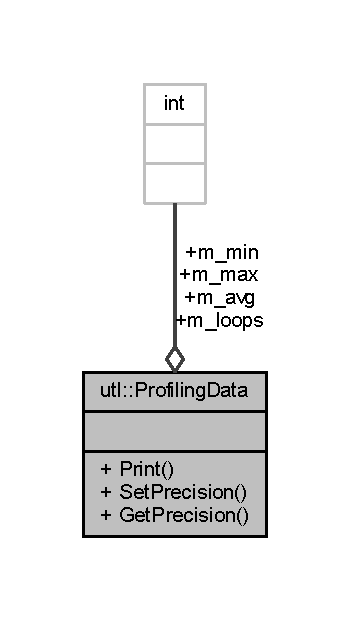
\includegraphics[width=168pt]{structutl_1_1_profiling_data__coll__graph}
\end{center}
\end{figure}
\subsection*{Public Member Functions}
\begin{DoxyCompactItemize}
\item 
void \mbox{\hyperlink{structutl_1_1_profiling_data_abf6ff992cd66ef1ad903afc3d3057d2e}{print}} () const
\item 
void \mbox{\hyperlink{structutl_1_1_profiling_data_a56c49476d775e0c82d5718f609680a5e}{set\+Precision}} (\mbox{\hyperlink{namespaceutl_ad221bb3fac593651670bdc0263b92707}{Profiling\+Precision}} precision)
\item 
\mbox{\hyperlink{namespaceutl_ad221bb3fac593651670bdc0263b92707}{Profiling\+Precision}} \mbox{\hyperlink{structutl_1_1_profiling_data_a81bcb78d3bb5fdb2ef0e100e44fed249}{get\+Precision}} () const
\end{DoxyCompactItemize}
\subsection*{Public Attributes}
\begin{DoxyCompactItemize}
\item 
unsigned int \mbox{\hyperlink{structutl_1_1_profiling_data_a1262c85d877f95e243991d5d82e8aa3f}{m\+\_\+loops}}
\item 
unsigned int \mbox{\hyperlink{structutl_1_1_profiling_data_a61e7406f3b528d1740ce266673cc725b}{m\+\_\+min}}
\item 
unsigned int \mbox{\hyperlink{structutl_1_1_profiling_data_aa37adf9f2cd78f78d581b1bf12130910}{m\+\_\+avg}}
\item 
unsigned int \mbox{\hyperlink{structutl_1_1_profiling_data_a5590a66a5ce2b5850ca8053ce62b4edc}{m\+\_\+max}}
\end{DoxyCompactItemize}


\subsection{Member Function Documentation}
\mbox{\Hypertarget{structutl_1_1_profiling_data_a81bcb78d3bb5fdb2ef0e100e44fed249}\label{structutl_1_1_profiling_data_a81bcb78d3bb5fdb2ef0e100e44fed249}} 
\index{utl\+::\+Profiling\+Data@{utl\+::\+Profiling\+Data}!get\+Precision@{get\+Precision}}
\index{get\+Precision@{get\+Precision}!utl\+::\+Profiling\+Data@{utl\+::\+Profiling\+Data}}
\subsubsection{\texorpdfstring{get\+Precision()}{getPrecision()}}
{\footnotesize\ttfamily \mbox{\hyperlink{namespaceutl_ad221bb3fac593651670bdc0263b92707}{utl\+::\+Profiling\+Precision}} utl\+::\+Profiling\+Data\+::get\+Precision (\begin{DoxyParamCaption}{ }\end{DoxyParamCaption}) const}

\mbox{\Hypertarget{structutl_1_1_profiling_data_abf6ff992cd66ef1ad903afc3d3057d2e}\label{structutl_1_1_profiling_data_abf6ff992cd66ef1ad903afc3d3057d2e}} 
\index{utl\+::\+Profiling\+Data@{utl\+::\+Profiling\+Data}!print@{print}}
\index{print@{print}!utl\+::\+Profiling\+Data@{utl\+::\+Profiling\+Data}}
\subsubsection{\texorpdfstring{print()}{print()}}
{\footnotesize\ttfamily void utl\+::\+Profiling\+Data\+::print (\begin{DoxyParamCaption}{ }\end{DoxyParamCaption}) const}

\mbox{\Hypertarget{structutl_1_1_profiling_data_a56c49476d775e0c82d5718f609680a5e}\label{structutl_1_1_profiling_data_a56c49476d775e0c82d5718f609680a5e}} 
\index{utl\+::\+Profiling\+Data@{utl\+::\+Profiling\+Data}!set\+Precision@{set\+Precision}}
\index{set\+Precision@{set\+Precision}!utl\+::\+Profiling\+Data@{utl\+::\+Profiling\+Data}}
\subsubsection{\texorpdfstring{set\+Precision()}{setPrecision()}}
{\footnotesize\ttfamily void utl\+::\+Profiling\+Data\+::set\+Precision (\begin{DoxyParamCaption}\item[{\mbox{\hyperlink{namespaceutl_ad221bb3fac593651670bdc0263b92707}{Profiling\+Precision}}}]{precision }\end{DoxyParamCaption})}



\subsection{Member Data Documentation}
\mbox{\Hypertarget{structutl_1_1_profiling_data_aa37adf9f2cd78f78d581b1bf12130910}\label{structutl_1_1_profiling_data_aa37adf9f2cd78f78d581b1bf12130910}} 
\index{utl\+::\+Profiling\+Data@{utl\+::\+Profiling\+Data}!m\+\_\+avg@{m\+\_\+avg}}
\index{m\+\_\+avg@{m\+\_\+avg}!utl\+::\+Profiling\+Data@{utl\+::\+Profiling\+Data}}
\subsubsection{\texorpdfstring{m\+\_\+avg}{m\_avg}}
{\footnotesize\ttfamily unsigned int utl\+::\+Profiling\+Data\+::m\+\_\+avg}

\mbox{\Hypertarget{structutl_1_1_profiling_data_a1262c85d877f95e243991d5d82e8aa3f}\label{structutl_1_1_profiling_data_a1262c85d877f95e243991d5d82e8aa3f}} 
\index{utl\+::\+Profiling\+Data@{utl\+::\+Profiling\+Data}!m\+\_\+loops@{m\+\_\+loops}}
\index{m\+\_\+loops@{m\+\_\+loops}!utl\+::\+Profiling\+Data@{utl\+::\+Profiling\+Data}}
\subsubsection{\texorpdfstring{m\+\_\+loops}{m\_loops}}
{\footnotesize\ttfamily unsigned int utl\+::\+Profiling\+Data\+::m\+\_\+loops}

\mbox{\Hypertarget{structutl_1_1_profiling_data_a5590a66a5ce2b5850ca8053ce62b4edc}\label{structutl_1_1_profiling_data_a5590a66a5ce2b5850ca8053ce62b4edc}} 
\index{utl\+::\+Profiling\+Data@{utl\+::\+Profiling\+Data}!m\+\_\+max@{m\+\_\+max}}
\index{m\+\_\+max@{m\+\_\+max}!utl\+::\+Profiling\+Data@{utl\+::\+Profiling\+Data}}
\subsubsection{\texorpdfstring{m\+\_\+max}{m\_max}}
{\footnotesize\ttfamily unsigned int utl\+::\+Profiling\+Data\+::m\+\_\+max}

\mbox{\Hypertarget{structutl_1_1_profiling_data_a61e7406f3b528d1740ce266673cc725b}\label{structutl_1_1_profiling_data_a61e7406f3b528d1740ce266673cc725b}} 
\index{utl\+::\+Profiling\+Data@{utl\+::\+Profiling\+Data}!m\+\_\+min@{m\+\_\+min}}
\index{m\+\_\+min@{m\+\_\+min}!utl\+::\+Profiling\+Data@{utl\+::\+Profiling\+Data}}
\subsubsection{\texorpdfstring{m\+\_\+min}{m\_min}}
{\footnotesize\ttfamily unsigned int utl\+::\+Profiling\+Data\+::m\+\_\+min}



The documentation for this struct was generated from the following files\+:\begin{DoxyCompactItemize}
\item 
D\+:/\+Library/\+Documents/\+Job/\+Forschungsmaster/\+Projekte/\+Eye\+Candy3\+D/\+Eye\+Candy3\+D/include/\+E\+C3\+D/\+Utilities/\mbox{\hyperlink{_profiler_8h}{Profiler.\+h}}\item 
D\+:/\+Library/\+Documents/\+Job/\+Forschungsmaster/\+Projekte/\+Eye\+Candy3\+D/\+Eye\+Candy3\+D/src/\+Utilities/\mbox{\hyperlink{_profiler_8cpp}{Profiler.\+cpp}}\end{DoxyCompactItemize}

\hypertarget{classngl__gui_1_1_radio_button}{}\section{ngl\+\_\+gui\+:\+:Radio\+Button Class Reference}
\label{classngl__gui_1_1_radio_button}\index{ngl\+\_\+gui\+::\+Radio\+Button@{ngl\+\_\+gui\+::\+Radio\+Button}}


{\ttfamily \#include $<$Radio\+Button.\+h$>$}



Inheritance diagram for ngl\+\_\+gui\+:\+:Radio\+Button\+:\nopagebreak
\begin{figure}[H]
\begin{center}
\leavevmode
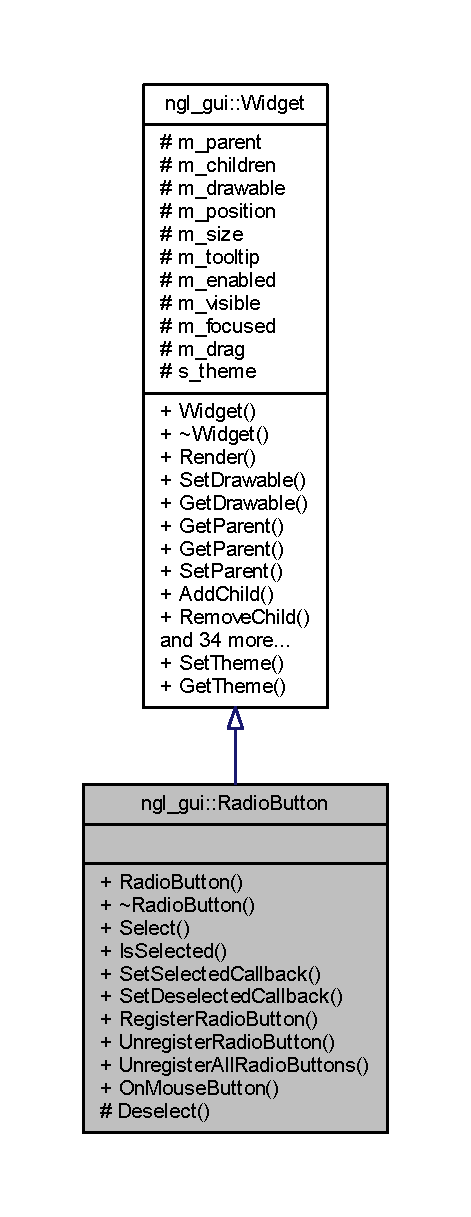
\includegraphics[height=550pt]{classngl__gui_1_1_radio_button__inherit__graph}
\end{center}
\end{figure}


Collaboration diagram for ngl\+\_\+gui\+:\+:Radio\+Button\+:
\nopagebreak
\begin{figure}[H]
\begin{center}
\leavevmode
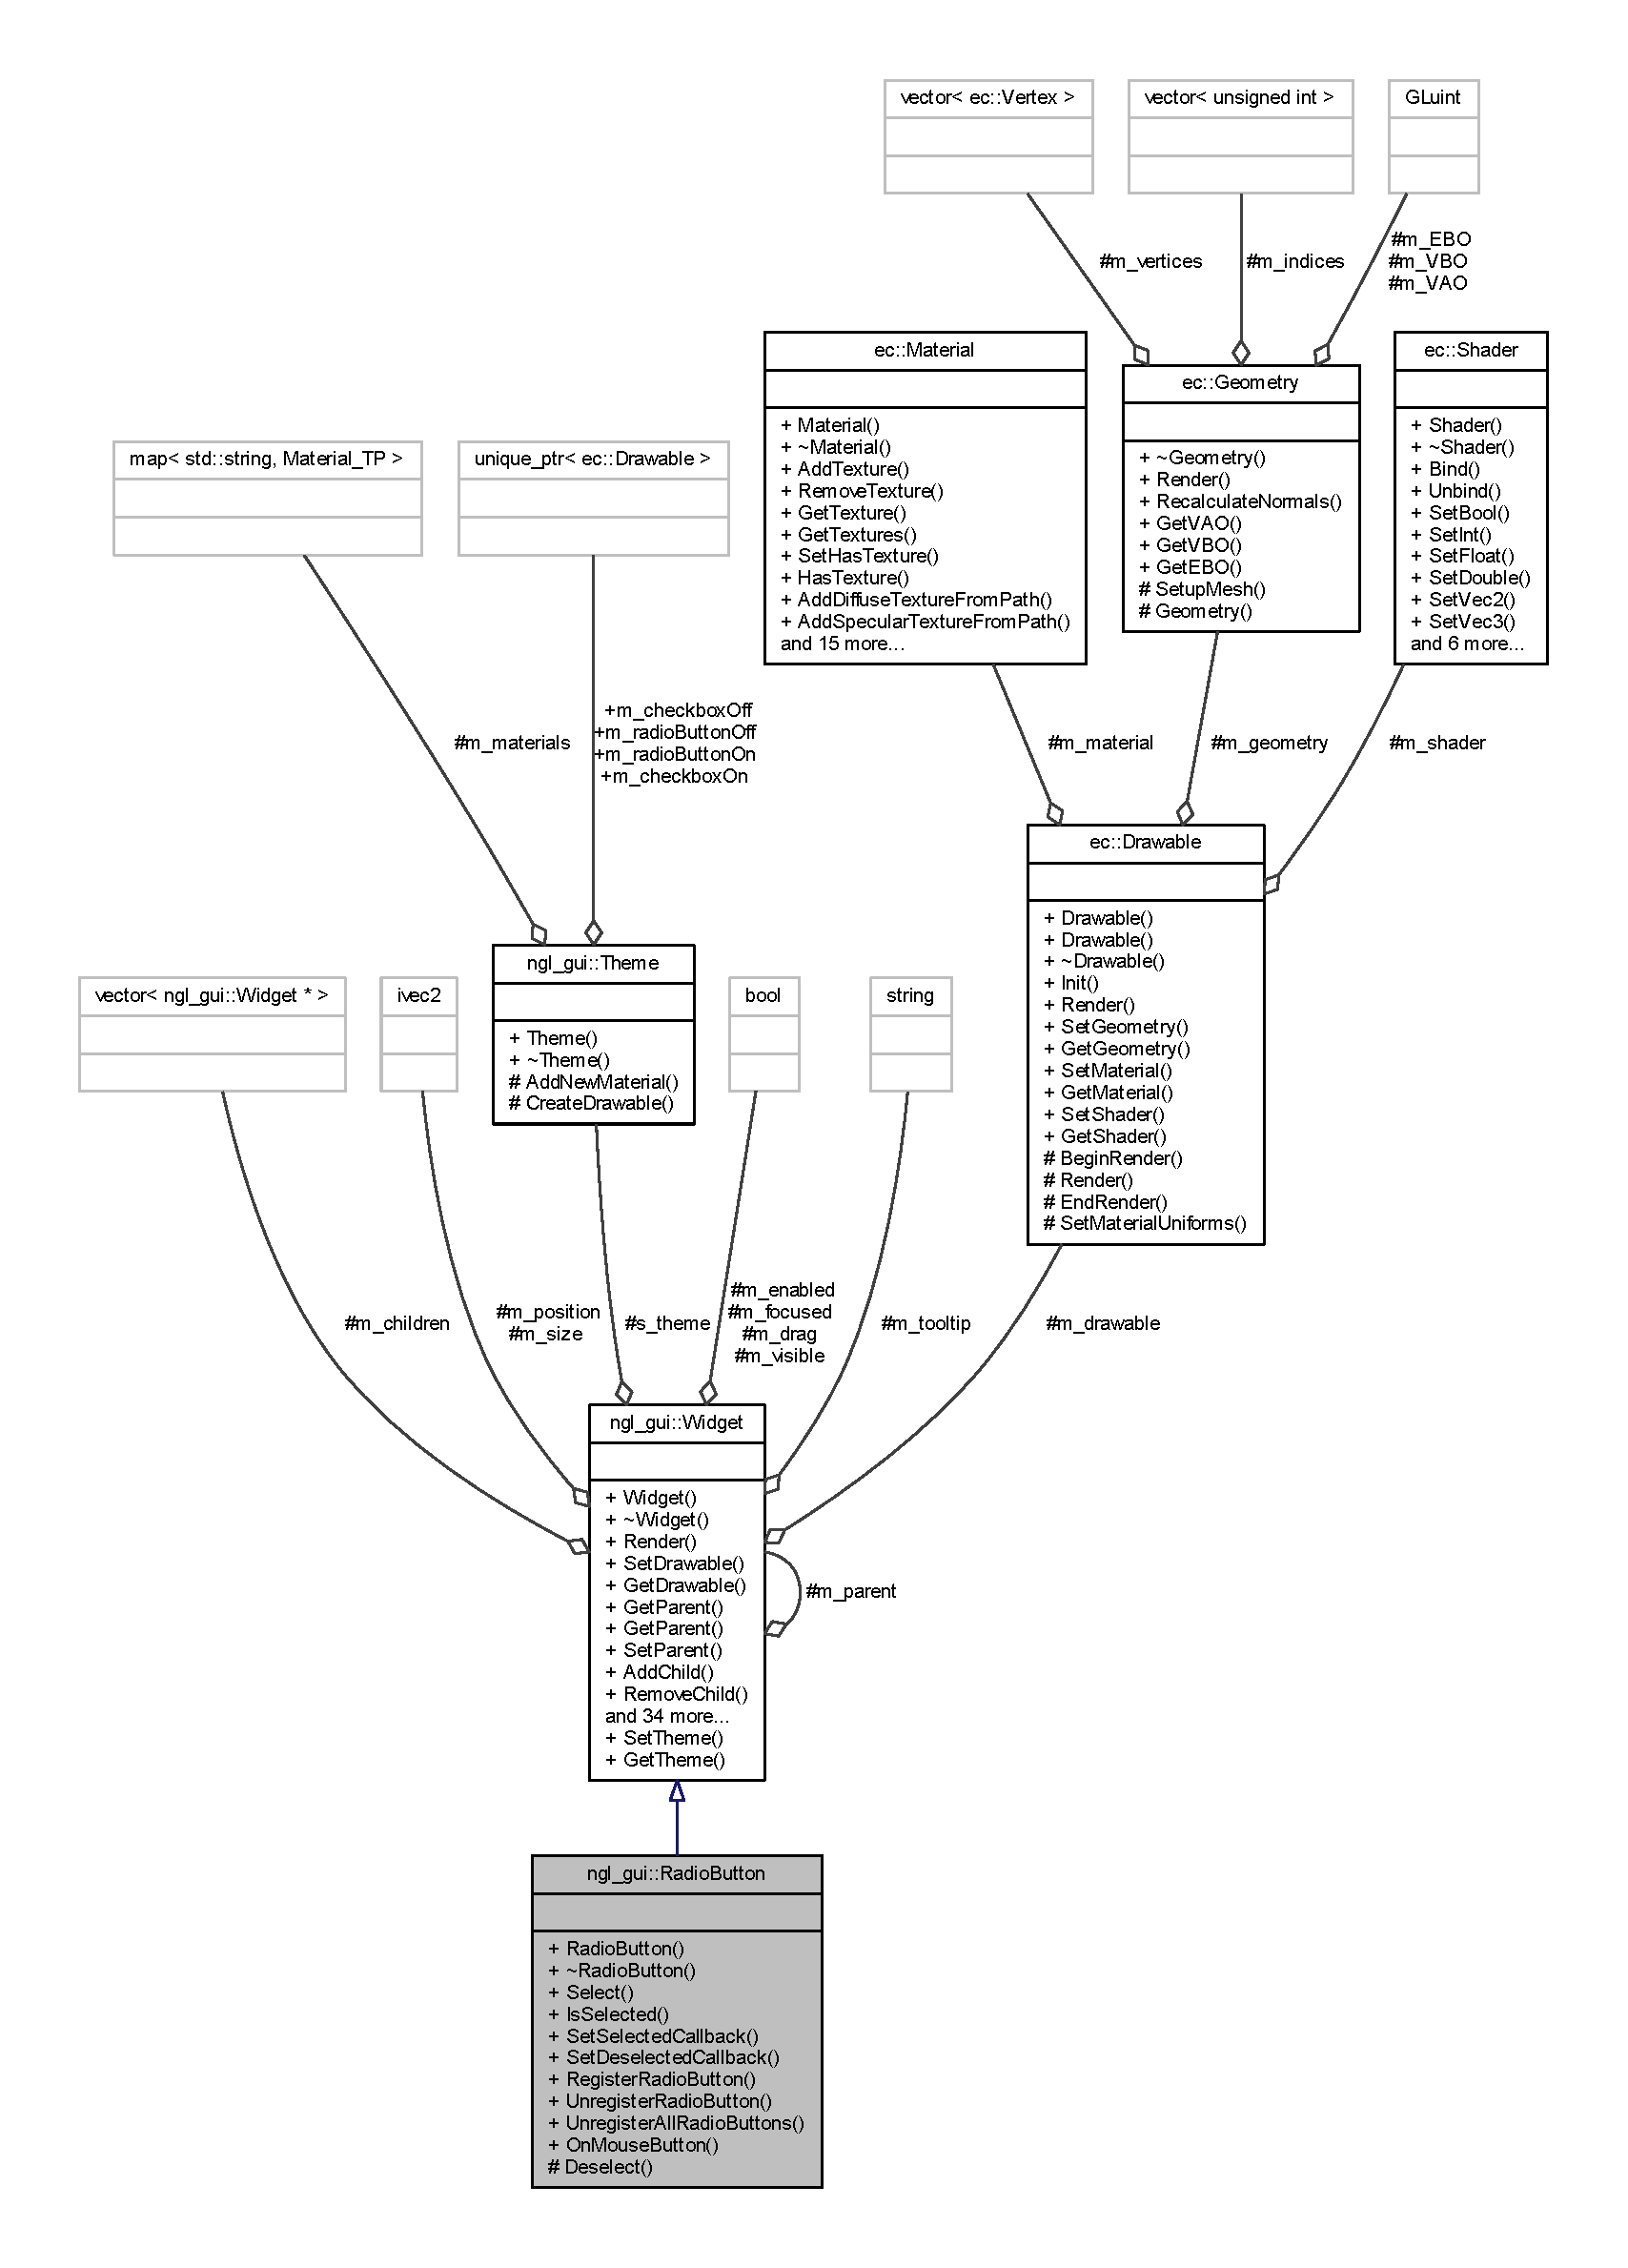
\includegraphics[width=350pt]{classngl__gui_1_1_radio_button__coll__graph}
\end{center}
\end{figure}
\subsection*{Public Member Functions}
\begin{DoxyCompactItemize}
\item 
\mbox{\hyperlink{classngl__gui_1_1_radio_button_a919cbf40d57d74418b5a38fe4e6754f2}{Radio\+Button}} (\mbox{\hyperlink{classngl__gui_1_1_widget}{Widget}} $\ast$parent)
\item 
virtual \mbox{\hyperlink{classngl__gui_1_1_radio_button_ab31789870bcefcfc9abc45fa3881a2ef}{$\sim$\+Radio\+Button}} ()
\item 
void \mbox{\hyperlink{classngl__gui_1_1_radio_button_a175e3625d976ea82c99c16f6fa64a5fb}{Select}} ()
\item 
bool \mbox{\hyperlink{classngl__gui_1_1_radio_button_aee5f82544897695560fac4cfa7359016}{Is\+Selected}} () const
\item 
void \mbox{\hyperlink{classngl__gui_1_1_radio_button_a7144c9e2b802a37b829587961314a97e}{Set\+Selected\+Callback}} (std\+::function$<$ void()$>$ callback)
\item 
void \mbox{\hyperlink{classngl__gui_1_1_radio_button_a70e72c9cdba8b96ad0e82f0a3a17b866}{Set\+Deselected\+Callback}} (std\+::function$<$ void()$>$ callback)
\item 
bool \mbox{\hyperlink{classngl__gui_1_1_radio_button_a29196e626ecf49500341062368503de5}{Register\+Radio\+Button}} (\mbox{\hyperlink{classngl__gui_1_1_radio_button}{Radio\+Button}} $\ast$radio\+Button)
\item 
bool \mbox{\hyperlink{classngl__gui_1_1_radio_button_a57b54123f1c2a144ff54dd3b0713e50b}{Unregister\+Radio\+Button}} (\mbox{\hyperlink{classngl__gui_1_1_radio_button}{Radio\+Button}} $\ast$radio\+Button)
\item 
void \mbox{\hyperlink{classngl__gui_1_1_radio_button_a7cf170dd3058219c27abea20249fdc07}{Unregister\+All\+Radio\+Buttons}} ()
\item 
virtual bool \mbox{\hyperlink{classngl__gui_1_1_radio_button_ab1593ae6fbd370c89c6c862a4ee58a92}{On\+Mouse\+Button}} (const glm\+::ivec2 \&position, int button, int mods, bool pressed) override
\end{DoxyCompactItemize}
\subsection*{Protected Member Functions}
\begin{DoxyCompactItemize}
\item 
void \mbox{\hyperlink{classngl__gui_1_1_radio_button_a53a5262bd865fafade28fe859bcd1b4e}{Deselect}} ()
\end{DoxyCompactItemize}
\subsection*{Additional Inherited Members}


\subsection{Constructor \& Destructor Documentation}
\mbox{\Hypertarget{classngl__gui_1_1_radio_button_a919cbf40d57d74418b5a38fe4e6754f2}\label{classngl__gui_1_1_radio_button_a919cbf40d57d74418b5a38fe4e6754f2}} 
\index{ngl\+\_\+gui\+::\+Radio\+Button@{ngl\+\_\+gui\+::\+Radio\+Button}!Radio\+Button@{Radio\+Button}}
\index{Radio\+Button@{Radio\+Button}!ngl\+\_\+gui\+::\+Radio\+Button@{ngl\+\_\+gui\+::\+Radio\+Button}}
\subsubsection{\texorpdfstring{Radio\+Button()}{RadioButton()}}
{\footnotesize\ttfamily ngl\+\_\+gui\+::\+Radio\+Button\+::\+Radio\+Button (\begin{DoxyParamCaption}\item[{\mbox{\hyperlink{classngl__gui_1_1_widget}{Widget}} $\ast$}]{parent }\end{DoxyParamCaption})\hspace{0.3cm}{\ttfamily [explicit]}}

\mbox{\Hypertarget{classngl__gui_1_1_radio_button_ab31789870bcefcfc9abc45fa3881a2ef}\label{classngl__gui_1_1_radio_button_ab31789870bcefcfc9abc45fa3881a2ef}} 
\index{ngl\+\_\+gui\+::\+Radio\+Button@{ngl\+\_\+gui\+::\+Radio\+Button}!````~Radio\+Button@{$\sim$\+Radio\+Button}}
\index{````~Radio\+Button@{$\sim$\+Radio\+Button}!ngl\+\_\+gui\+::\+Radio\+Button@{ngl\+\_\+gui\+::\+Radio\+Button}}
\subsubsection{\texorpdfstring{$\sim$\+Radio\+Button()}{~RadioButton()}}
{\footnotesize\ttfamily ngl\+\_\+gui\+::\+Radio\+Button\+::$\sim$\+Radio\+Button (\begin{DoxyParamCaption}{ }\end{DoxyParamCaption})\hspace{0.3cm}{\ttfamily [virtual]}}



\subsection{Member Function Documentation}
\mbox{\Hypertarget{classngl__gui_1_1_radio_button_a53a5262bd865fafade28fe859bcd1b4e}\label{classngl__gui_1_1_radio_button_a53a5262bd865fafade28fe859bcd1b4e}} 
\index{ngl\+\_\+gui\+::\+Radio\+Button@{ngl\+\_\+gui\+::\+Radio\+Button}!Deselect@{Deselect}}
\index{Deselect@{Deselect}!ngl\+\_\+gui\+::\+Radio\+Button@{ngl\+\_\+gui\+::\+Radio\+Button}}
\subsubsection{\texorpdfstring{Deselect()}{Deselect()}}
{\footnotesize\ttfamily void ngl\+\_\+gui\+::\+Radio\+Button\+::\+Deselect (\begin{DoxyParamCaption}{ }\end{DoxyParamCaption})\hspace{0.3cm}{\ttfamily [protected]}}

\mbox{\Hypertarget{classngl__gui_1_1_radio_button_aee5f82544897695560fac4cfa7359016}\label{classngl__gui_1_1_radio_button_aee5f82544897695560fac4cfa7359016}} 
\index{ngl\+\_\+gui\+::\+Radio\+Button@{ngl\+\_\+gui\+::\+Radio\+Button}!Is\+Selected@{Is\+Selected}}
\index{Is\+Selected@{Is\+Selected}!ngl\+\_\+gui\+::\+Radio\+Button@{ngl\+\_\+gui\+::\+Radio\+Button}}
\subsubsection{\texorpdfstring{Is\+Selected()}{IsSelected()}}
{\footnotesize\ttfamily bool ngl\+\_\+gui\+::\+Radio\+Button\+::\+Is\+Selected (\begin{DoxyParamCaption}{ }\end{DoxyParamCaption}) const}

\mbox{\Hypertarget{classngl__gui_1_1_radio_button_ab1593ae6fbd370c89c6c862a4ee58a92}\label{classngl__gui_1_1_radio_button_ab1593ae6fbd370c89c6c862a4ee58a92}} 
\index{ngl\+\_\+gui\+::\+Radio\+Button@{ngl\+\_\+gui\+::\+Radio\+Button}!On\+Mouse\+Button@{On\+Mouse\+Button}}
\index{On\+Mouse\+Button@{On\+Mouse\+Button}!ngl\+\_\+gui\+::\+Radio\+Button@{ngl\+\_\+gui\+::\+Radio\+Button}}
\subsubsection{\texorpdfstring{On\+Mouse\+Button()}{OnMouseButton()}}
{\footnotesize\ttfamily bool ngl\+\_\+gui\+::\+Radio\+Button\+::\+On\+Mouse\+Button (\begin{DoxyParamCaption}\item[{const glm\+::ivec2 \&}]{position,  }\item[{int}]{button,  }\item[{int}]{mods,  }\item[{bool}]{pressed }\end{DoxyParamCaption})\hspace{0.3cm}{\ttfamily [override]}, {\ttfamily [virtual]}}



Reimplemented from \mbox{\hyperlink{classngl__gui_1_1_widget_a721b18dc7a09b0b7b4ff0c02162409b8}{ngl\+\_\+gui\+::\+Widget}}.

\mbox{\Hypertarget{classngl__gui_1_1_radio_button_a29196e626ecf49500341062368503de5}\label{classngl__gui_1_1_radio_button_a29196e626ecf49500341062368503de5}} 
\index{ngl\+\_\+gui\+::\+Radio\+Button@{ngl\+\_\+gui\+::\+Radio\+Button}!Register\+Radio\+Button@{Register\+Radio\+Button}}
\index{Register\+Radio\+Button@{Register\+Radio\+Button}!ngl\+\_\+gui\+::\+Radio\+Button@{ngl\+\_\+gui\+::\+Radio\+Button}}
\subsubsection{\texorpdfstring{Register\+Radio\+Button()}{RegisterRadioButton()}}
{\footnotesize\ttfamily bool ngl\+\_\+gui\+::\+Radio\+Button\+::\+Register\+Radio\+Button (\begin{DoxyParamCaption}\item[{\mbox{\hyperlink{classngl__gui_1_1_radio_button}{Radio\+Button}} $\ast$}]{radio\+Button }\end{DoxyParamCaption})}

\mbox{\Hypertarget{classngl__gui_1_1_radio_button_a175e3625d976ea82c99c16f6fa64a5fb}\label{classngl__gui_1_1_radio_button_a175e3625d976ea82c99c16f6fa64a5fb}} 
\index{ngl\+\_\+gui\+::\+Radio\+Button@{ngl\+\_\+gui\+::\+Radio\+Button}!Select@{Select}}
\index{Select@{Select}!ngl\+\_\+gui\+::\+Radio\+Button@{ngl\+\_\+gui\+::\+Radio\+Button}}
\subsubsection{\texorpdfstring{Select()}{Select()}}
{\footnotesize\ttfamily void ngl\+\_\+gui\+::\+Radio\+Button\+::\+Select (\begin{DoxyParamCaption}{ }\end{DoxyParamCaption})}

\mbox{\Hypertarget{classngl__gui_1_1_radio_button_a70e72c9cdba8b96ad0e82f0a3a17b866}\label{classngl__gui_1_1_radio_button_a70e72c9cdba8b96ad0e82f0a3a17b866}} 
\index{ngl\+\_\+gui\+::\+Radio\+Button@{ngl\+\_\+gui\+::\+Radio\+Button}!Set\+Deselected\+Callback@{Set\+Deselected\+Callback}}
\index{Set\+Deselected\+Callback@{Set\+Deselected\+Callback}!ngl\+\_\+gui\+::\+Radio\+Button@{ngl\+\_\+gui\+::\+Radio\+Button}}
\subsubsection{\texorpdfstring{Set\+Deselected\+Callback()}{SetDeselectedCallback()}}
{\footnotesize\ttfamily void ngl\+\_\+gui\+::\+Radio\+Button\+::\+Set\+Deselected\+Callback (\begin{DoxyParamCaption}\item[{std\+::function$<$ void()$>$}]{callback }\end{DoxyParamCaption})}

\mbox{\Hypertarget{classngl__gui_1_1_radio_button_a7144c9e2b802a37b829587961314a97e}\label{classngl__gui_1_1_radio_button_a7144c9e2b802a37b829587961314a97e}} 
\index{ngl\+\_\+gui\+::\+Radio\+Button@{ngl\+\_\+gui\+::\+Radio\+Button}!Set\+Selected\+Callback@{Set\+Selected\+Callback}}
\index{Set\+Selected\+Callback@{Set\+Selected\+Callback}!ngl\+\_\+gui\+::\+Radio\+Button@{ngl\+\_\+gui\+::\+Radio\+Button}}
\subsubsection{\texorpdfstring{Set\+Selected\+Callback()}{SetSelectedCallback()}}
{\footnotesize\ttfamily void ngl\+\_\+gui\+::\+Radio\+Button\+::\+Set\+Selected\+Callback (\begin{DoxyParamCaption}\item[{std\+::function$<$ void()$>$}]{callback }\end{DoxyParamCaption})}

\mbox{\Hypertarget{classngl__gui_1_1_radio_button_a7cf170dd3058219c27abea20249fdc07}\label{classngl__gui_1_1_radio_button_a7cf170dd3058219c27abea20249fdc07}} 
\index{ngl\+\_\+gui\+::\+Radio\+Button@{ngl\+\_\+gui\+::\+Radio\+Button}!Unregister\+All\+Radio\+Buttons@{Unregister\+All\+Radio\+Buttons}}
\index{Unregister\+All\+Radio\+Buttons@{Unregister\+All\+Radio\+Buttons}!ngl\+\_\+gui\+::\+Radio\+Button@{ngl\+\_\+gui\+::\+Radio\+Button}}
\subsubsection{\texorpdfstring{Unregister\+All\+Radio\+Buttons()}{UnregisterAllRadioButtons()}}
{\footnotesize\ttfamily void ngl\+\_\+gui\+::\+Radio\+Button\+::\+Unregister\+All\+Radio\+Buttons (\begin{DoxyParamCaption}{ }\end{DoxyParamCaption})}

\mbox{\Hypertarget{classngl__gui_1_1_radio_button_a57b54123f1c2a144ff54dd3b0713e50b}\label{classngl__gui_1_1_radio_button_a57b54123f1c2a144ff54dd3b0713e50b}} 
\index{ngl\+\_\+gui\+::\+Radio\+Button@{ngl\+\_\+gui\+::\+Radio\+Button}!Unregister\+Radio\+Button@{Unregister\+Radio\+Button}}
\index{Unregister\+Radio\+Button@{Unregister\+Radio\+Button}!ngl\+\_\+gui\+::\+Radio\+Button@{ngl\+\_\+gui\+::\+Radio\+Button}}
\subsubsection{\texorpdfstring{Unregister\+Radio\+Button()}{UnregisterRadioButton()}}
{\footnotesize\ttfamily bool ngl\+\_\+gui\+::\+Radio\+Button\+::\+Unregister\+Radio\+Button (\begin{DoxyParamCaption}\item[{\mbox{\hyperlink{classngl__gui_1_1_radio_button}{Radio\+Button}} $\ast$}]{radio\+Button }\end{DoxyParamCaption})}



The documentation for this class was generated from the following files\+:\begin{DoxyCompactItemize}
\item 
D\+:/\+Library/\+Documents/\+Job/\+Forschungsmaster/\+Projekte/\+Eye\+Candy3\+D/\+Eye\+Candy3\+D/include/\+E\+C3\+D/\+G\+U\+I/\mbox{\hyperlink{_radio_button_8h}{Radio\+Button.\+h}}\item 
D\+:/\+Library/\+Documents/\+Job/\+Forschungsmaster/\+Projekte/\+Eye\+Candy3\+D/\+Eye\+Candy3\+D/src/\+G\+U\+I/\mbox{\hyperlink{_radio_button_8cpp}{Radio\+Button.\+cpp}}\end{DoxyCompactItemize}

\hypertarget{classec_1_1_rectangle_mesh}{}\section{ec\+:\+:Rectangle\+Mesh Class Reference}
\label{classec_1_1_rectangle_mesh}\index{ec\+::\+Rectangle\+Mesh@{ec\+::\+Rectangle\+Mesh}}


{\ttfamily \#include $<$Rectangle\+Mesh.\+h$>$}



Inheritance diagram for ec\+:\+:Rectangle\+Mesh\+:
\nopagebreak
\begin{figure}[H]
\begin{center}
\leavevmode
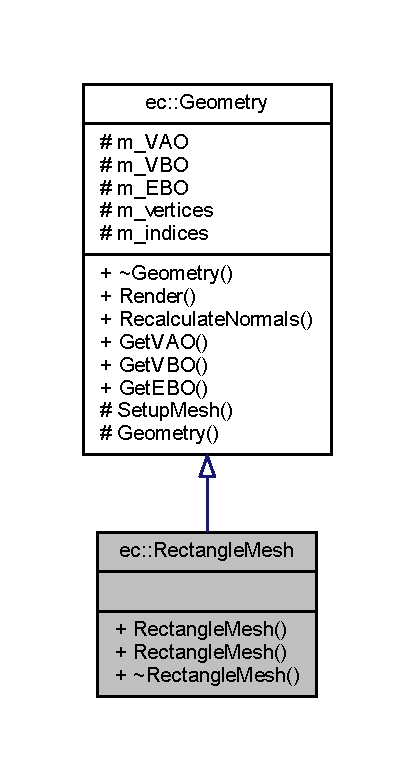
\includegraphics[width=199pt]{classec_1_1_rectangle_mesh__inherit__graph}
\end{center}
\end{figure}


Collaboration diagram for ec\+:\+:Rectangle\+Mesh\+:
\nopagebreak
\begin{figure}[H]
\begin{center}
\leavevmode
\includegraphics[width=350pt]{classec_1_1_rectangle_mesh__coll__graph}
\end{center}
\end{figure}
\subsection*{Public Member Functions}
\begin{DoxyCompactItemize}
\item 
\mbox{\hyperlink{classec_1_1_rectangle_mesh_aa75e834f688d15a8ec8162e7a9ed1c05}{Rectangle\+Mesh}} (const float uniform=1.\+0f)
\item 
\mbox{\hyperlink{classec_1_1_rectangle_mesh_a7fe73fb3ef2979cb3d7230aaeffeecdd}{Rectangle\+Mesh}} (const float width, const float height)
\item 
virtual \mbox{\hyperlink{classec_1_1_rectangle_mesh_a520388a70dadc70155b2ade95f06d110}{$\sim$\+Rectangle\+Mesh}} ()
\end{DoxyCompactItemize}
\subsection*{Additional Inherited Members}


\subsection{Constructor \& Destructor Documentation}
\mbox{\Hypertarget{classec_1_1_rectangle_mesh_aa75e834f688d15a8ec8162e7a9ed1c05}\label{classec_1_1_rectangle_mesh_aa75e834f688d15a8ec8162e7a9ed1c05}} 
\index{ec\+::\+Rectangle\+Mesh@{ec\+::\+Rectangle\+Mesh}!Rectangle\+Mesh@{Rectangle\+Mesh}}
\index{Rectangle\+Mesh@{Rectangle\+Mesh}!ec\+::\+Rectangle\+Mesh@{ec\+::\+Rectangle\+Mesh}}
\subsubsection{\texorpdfstring{Rectangle\+Mesh()}{RectangleMesh()}\hspace{0.1cm}{\footnotesize\ttfamily [1/2]}}
{\footnotesize\ttfamily ec\+::\+Rectangle\+Mesh\+::\+Rectangle\+Mesh (\begin{DoxyParamCaption}\item[{const float}]{uniform = {\ttfamily 1.0f} }\end{DoxyParamCaption})\hspace{0.3cm}{\ttfamily [explicit]}}

\mbox{\Hypertarget{classec_1_1_rectangle_mesh_a7fe73fb3ef2979cb3d7230aaeffeecdd}\label{classec_1_1_rectangle_mesh_a7fe73fb3ef2979cb3d7230aaeffeecdd}} 
\index{ec\+::\+Rectangle\+Mesh@{ec\+::\+Rectangle\+Mesh}!Rectangle\+Mesh@{Rectangle\+Mesh}}
\index{Rectangle\+Mesh@{Rectangle\+Mesh}!ec\+::\+Rectangle\+Mesh@{ec\+::\+Rectangle\+Mesh}}
\subsubsection{\texorpdfstring{Rectangle\+Mesh()}{RectangleMesh()}\hspace{0.1cm}{\footnotesize\ttfamily [2/2]}}
{\footnotesize\ttfamily ec\+::\+Rectangle\+Mesh\+::\+Rectangle\+Mesh (\begin{DoxyParamCaption}\item[{const float}]{width,  }\item[{const float}]{height }\end{DoxyParamCaption})\hspace{0.3cm}{\ttfamily [explicit]}}

\mbox{\Hypertarget{classec_1_1_rectangle_mesh_a520388a70dadc70155b2ade95f06d110}\label{classec_1_1_rectangle_mesh_a520388a70dadc70155b2ade95f06d110}} 
\index{ec\+::\+Rectangle\+Mesh@{ec\+::\+Rectangle\+Mesh}!````~Rectangle\+Mesh@{$\sim$\+Rectangle\+Mesh}}
\index{````~Rectangle\+Mesh@{$\sim$\+Rectangle\+Mesh}!ec\+::\+Rectangle\+Mesh@{ec\+::\+Rectangle\+Mesh}}
\subsubsection{\texorpdfstring{$\sim$\+Rectangle\+Mesh()}{~RectangleMesh()}}
{\footnotesize\ttfamily ec\+::\+Rectangle\+Mesh\+::$\sim$\+Rectangle\+Mesh (\begin{DoxyParamCaption}{ }\end{DoxyParamCaption})\hspace{0.3cm}{\ttfamily [virtual]}}



The documentation for this class was generated from the following files\+:\begin{DoxyCompactItemize}
\item 
D\+:/\+Library/\+Documents/\+Job/\+Forschungsmaster/\+Projekte/\+Eye\+Candy3\+D/\+Eye\+Candy3\+D/include/\+E\+C3\+D/\+Core/\mbox{\hyperlink{_rectangle_mesh_8h}{Rectangle\+Mesh.\+h}}\item 
D\+:/\+Library/\+Documents/\+Job/\+Forschungsmaster/\+Projekte/\+Eye\+Candy3\+D/\+Eye\+Candy3\+D/src/\+Core/\mbox{\hyperlink{_rectangle_mesh_8cpp}{Rectangle\+Mesh.\+cpp}}\end{DoxyCompactItemize}

\hypertarget{classec_1_1_renderer}{}\section{ec\+:\+:Renderer Class Reference}
\label{classec_1_1_renderer}\index{ec\+::\+Renderer@{ec\+::\+Renderer}}


A \mbox{\hyperlink{classec_1_1_renderer}{Renderer}} is responsible for rendering storing and using scene renderers.  




{\ttfamily \#include $<$Renderer.\+h$>$}



Collaboration diagram for ec\+:\+:Renderer\+:\nopagebreak
\begin{figure}[H]
\begin{center}
\leavevmode
\includegraphics[width=350pt]{classec_1_1_renderer__coll__graph}
\end{center}
\end{figure}
\subsection*{Public Member Functions}
\begin{DoxyCompactItemize}
\item 
\mbox{\hyperlink{classec_1_1_renderer_a97bc5e3d5050aa98a24fec3669eab28b}{Renderer}} (\mbox{\hyperlink{classec_1_1_window}{Window}} $\ast$window)
\begin{DoxyCompactList}\small\item\em \mbox{\hyperlink{classec_1_1_renderer}{Renderer}} constructor. \end{DoxyCompactList}\item 
\mbox{\hyperlink{classec_1_1_renderer_ab0a97bd174127b670899477a576d1fe6}{$\sim$\+Renderer}} ()
\item 
void \mbox{\hyperlink{classec_1_1_renderer_acfa2ed0fd23f3f6e36de59302a0148ad}{init}} (\mbox{\hyperlink{classec_1_1_shader}{Shader}} $\ast$gui\+Shader, \mbox{\hyperlink{classec_1_1_shader}{Shader}} $\ast$text\+Shader) const
\item 
void \mbox{\hyperlink{classec_1_1_renderer_a6dcc619251e6e4ec7f088567cba6fd57}{tick}} ()
\begin{DoxyCompactList}\small\item\em Update all gui systems. \end{DoxyCompactList}\item 
void \mbox{\hyperlink{classec_1_1_renderer_a7ff2c9444ad5da2a6db3331f19cb12f9}{render}} () const
\begin{DoxyCompactList}\small\item\em Render to the currently active window. \end{DoxyCompactList}\item 
void \mbox{\hyperlink{classec_1_1_renderer_abb876cb59df2478b52926782e2d0a0a9}{change\+Renderer}} (const std\+::string \&name)
\begin{DoxyCompactList}\small\item\em Change to an active renderer with the given name. \end{DoxyCompactList}\item 
void \mbox{\hyperlink{classec_1_1_renderer_aff1e2f129ce6b24a5ed1e27730a13762}{change\+Renderer}} (\mbox{\hyperlink{classec_1_1_scene_renderer}{Scene\+Renderer}} $\ast$renderer)
\begin{DoxyCompactList}\small\item\em Change the current scene renderer to a given one. The given renderer doesn\textquotesingle{}t have to be registered. \end{DoxyCompactList}\item 
void \mbox{\hyperlink{classec_1_1_renderer_a5e40791070a8fcb7250b4544bdac8725}{register\+Scene\+Renderer}} (const std\+::string \&name, \mbox{\hyperlink{classec_1_1_scene_renderer}{Scene\+Renderer}} $\ast$renderer)
\begin{DoxyCompactList}\small\item\em Register a new scene renderer. \end{DoxyCompactList}\item 
\mbox{\hyperlink{classec_1_1_scene_renderer}{Scene\+Renderer}} $\ast$ \mbox{\hyperlink{classec_1_1_renderer_a5c853ee4c34b069cc8142db8409abac6}{unregister\+Scene\+Renderer}} (const std\+::string \&name)
\begin{DoxyCompactList}\small\item\em Unregister an already registered scene renderer with the given name. \end{DoxyCompactList}\item 
\mbox{\hyperlink{classec_1_1_scene_renderer}{Scene\+Renderer}} $\ast$ \mbox{\hyperlink{classec_1_1_renderer_ab4e0c57f9d1f061f97e1fa188d52c477}{get\+Scene\+Renderer}} (const std\+::string \&name)
\begin{DoxyCompactList}\small\item\em Get a scene renderer with the given name. \end{DoxyCompactList}\end{DoxyCompactItemize}
\subsection*{Protected Member Functions}
\begin{DoxyCompactItemize}
\item 
void \mbox{\hyperlink{classec_1_1_renderer_a7dcfbdfd04d48452aba34a591b48341f}{render\+Gui}} () const
\begin{DoxyCompactList}\small\item\em Render the gui of every camera. \end{DoxyCompactList}\end{DoxyCompactItemize}
\subsection*{Protected Attributes}
\begin{DoxyCompactItemize}
\item 
\mbox{\hyperlink{classec_1_1_window}{Window}} $\ast$ \mbox{\hyperlink{classec_1_1_renderer_ac23d74f9d295bf833f095bdff8c8169b}{m\+\_\+window}}
\item 
\mbox{\hyperlink{classec_1_1_scene_renderer}{Scene\+Renderer}} $\ast$ \mbox{\hyperlink{classec_1_1_renderer_a00afed952025d62a654a5f961a55b342}{m\+\_\+active\+Renderer}}
\item 
\mbox{\hyperlink{classec_1_1_scene_renderer}{Scene\+Renderer}} $\ast$ \mbox{\hyperlink{classec_1_1_renderer_a818d84064fde8088d28358f7ea04f898}{m\+\_\+last\+Renderer}}
\item 
std\+::unique\+\_\+ptr$<$ \mbox{\hyperlink{classec_1_1_gui_renderer}{Gui\+Renderer}} $>$ \mbox{\hyperlink{classec_1_1_renderer_ac5969cd9baf68b5a3a02535bc9e9dd07}{m\+\_\+gui\+Renderer}}
\item 
std\+::map$<$ std\+::string, \mbox{\hyperlink{classec_1_1_scene_renderer}{Scene\+Renderer}} $\ast$ $>$ \mbox{\hyperlink{classec_1_1_renderer_ac3f0c1c3253fbac0f734af313cc410a4}{m\+\_\+renderer}}
\end{DoxyCompactItemize}


\subsection{Detailed Description}
A \mbox{\hyperlink{classec_1_1_renderer}{Renderer}} is responsible for rendering storing and using scene renderers. 

\subsection{Constructor \& Destructor Documentation}
\mbox{\Hypertarget{classec_1_1_renderer_a97bc5e3d5050aa98a24fec3669eab28b}\label{classec_1_1_renderer_a97bc5e3d5050aa98a24fec3669eab28b}} 
\index{ec\+::\+Renderer@{ec\+::\+Renderer}!Renderer@{Renderer}}
\index{Renderer@{Renderer}!ec\+::\+Renderer@{ec\+::\+Renderer}}
\subsubsection{\texorpdfstring{Renderer()}{Renderer()}}
{\footnotesize\ttfamily ec\+::\+Renderer\+::\+Renderer (\begin{DoxyParamCaption}\item[{\mbox{\hyperlink{classec_1_1_window}{Window}} $\ast$}]{window }\end{DoxyParamCaption})\hspace{0.3cm}{\ttfamily [explicit]}}



\mbox{\hyperlink{classec_1_1_renderer}{Renderer}} constructor. 


\begin{DoxyParams}{Parameters}
{\em window} & The window to render into \\
\hline
\end{DoxyParams}
\mbox{\Hypertarget{classec_1_1_renderer_ab0a97bd174127b670899477a576d1fe6}\label{classec_1_1_renderer_ab0a97bd174127b670899477a576d1fe6}} 
\index{ec\+::\+Renderer@{ec\+::\+Renderer}!````~Renderer@{$\sim$\+Renderer}}
\index{````~Renderer@{$\sim$\+Renderer}!ec\+::\+Renderer@{ec\+::\+Renderer}}
\subsubsection{\texorpdfstring{$\sim$\+Renderer()}{~Renderer()}}
{\footnotesize\ttfamily ec\+::\+Renderer\+::$\sim$\+Renderer (\begin{DoxyParamCaption}{ }\end{DoxyParamCaption})\hspace{0.3cm}{\ttfamily [default]}}



\subsection{Member Function Documentation}
\mbox{\Hypertarget{classec_1_1_renderer_abb876cb59df2478b52926782e2d0a0a9}\label{classec_1_1_renderer_abb876cb59df2478b52926782e2d0a0a9}} 
\index{ec\+::\+Renderer@{ec\+::\+Renderer}!change\+Renderer@{change\+Renderer}}
\index{change\+Renderer@{change\+Renderer}!ec\+::\+Renderer@{ec\+::\+Renderer}}
\subsubsection{\texorpdfstring{change\+Renderer()}{changeRenderer()}\hspace{0.1cm}{\footnotesize\ttfamily [1/2]}}
{\footnotesize\ttfamily void ec\+::\+Renderer\+::change\+Renderer (\begin{DoxyParamCaption}\item[{const std\+::string \&}]{name }\end{DoxyParamCaption})}



Change to an active renderer with the given name. 

The renderer has to be registered. \mbox{\Hypertarget{classec_1_1_renderer_aff1e2f129ce6b24a5ed1e27730a13762}\label{classec_1_1_renderer_aff1e2f129ce6b24a5ed1e27730a13762}} 
\index{ec\+::\+Renderer@{ec\+::\+Renderer}!change\+Renderer@{change\+Renderer}}
\index{change\+Renderer@{change\+Renderer}!ec\+::\+Renderer@{ec\+::\+Renderer}}
\subsubsection{\texorpdfstring{change\+Renderer()}{changeRenderer()}\hspace{0.1cm}{\footnotesize\ttfamily [2/2]}}
{\footnotesize\ttfamily void ec\+::\+Renderer\+::change\+Renderer (\begin{DoxyParamCaption}\item[{\mbox{\hyperlink{classec_1_1_scene_renderer}{Scene\+Renderer}} $\ast$}]{renderer }\end{DoxyParamCaption})}



Change the current scene renderer to a given one. The given renderer doesn\textquotesingle{}t have to be registered. 

\mbox{\Hypertarget{classec_1_1_renderer_ab4e0c57f9d1f061f97e1fa188d52c477}\label{classec_1_1_renderer_ab4e0c57f9d1f061f97e1fa188d52c477}} 
\index{ec\+::\+Renderer@{ec\+::\+Renderer}!get\+Scene\+Renderer@{get\+Scene\+Renderer}}
\index{get\+Scene\+Renderer@{get\+Scene\+Renderer}!ec\+::\+Renderer@{ec\+::\+Renderer}}
\subsubsection{\texorpdfstring{get\+Scene\+Renderer()}{getSceneRenderer()}}
{\footnotesize\ttfamily \mbox{\hyperlink{classec_1_1_scene_renderer}{ec\+::\+Scene\+Renderer}} $\ast$ ec\+::\+Renderer\+::get\+Scene\+Renderer (\begin{DoxyParamCaption}\item[{const std\+::string \&}]{name }\end{DoxyParamCaption})}



Get a scene renderer with the given name. 

\begin{DoxyReturn}{Returns}
The found scene renderer if it exist, nullptr otherwise. 
\end{DoxyReturn}
\mbox{\Hypertarget{classec_1_1_renderer_acfa2ed0fd23f3f6e36de59302a0148ad}\label{classec_1_1_renderer_acfa2ed0fd23f3f6e36de59302a0148ad}} 
\index{ec\+::\+Renderer@{ec\+::\+Renderer}!init@{init}}
\index{init@{init}!ec\+::\+Renderer@{ec\+::\+Renderer}}
\subsubsection{\texorpdfstring{init()}{init()}}
{\footnotesize\ttfamily void ec\+::\+Renderer\+::init (\begin{DoxyParamCaption}\item[{\mbox{\hyperlink{classec_1_1_shader}{Shader}} $\ast$}]{gui\+Shader,  }\item[{\mbox{\hyperlink{classec_1_1_shader}{Shader}} $\ast$}]{text\+Shader }\end{DoxyParamCaption}) const}

\mbox{\Hypertarget{classec_1_1_renderer_a5e40791070a8fcb7250b4544bdac8725}\label{classec_1_1_renderer_a5e40791070a8fcb7250b4544bdac8725}} 
\index{ec\+::\+Renderer@{ec\+::\+Renderer}!register\+Scene\+Renderer@{register\+Scene\+Renderer}}
\index{register\+Scene\+Renderer@{register\+Scene\+Renderer}!ec\+::\+Renderer@{ec\+::\+Renderer}}
\subsubsection{\texorpdfstring{register\+Scene\+Renderer()}{registerSceneRenderer()}}
{\footnotesize\ttfamily void ec\+::\+Renderer\+::register\+Scene\+Renderer (\begin{DoxyParamCaption}\item[{const std\+::string \&}]{name,  }\item[{\mbox{\hyperlink{classec_1_1_scene_renderer}{Scene\+Renderer}} $\ast$}]{renderer }\end{DoxyParamCaption})}



Register a new scene renderer. 


\begin{DoxyParams}{Parameters}
{\em name} & The id of the new registered renderer. \\
\hline
{\em renderer} & The new renderer to register. \\
\hline
\end{DoxyParams}
\mbox{\Hypertarget{classec_1_1_renderer_a7ff2c9444ad5da2a6db3331f19cb12f9}\label{classec_1_1_renderer_a7ff2c9444ad5da2a6db3331f19cb12f9}} 
\index{ec\+::\+Renderer@{ec\+::\+Renderer}!render@{render}}
\index{render@{render}!ec\+::\+Renderer@{ec\+::\+Renderer}}
\subsubsection{\texorpdfstring{render()}{render()}}
{\footnotesize\ttfamily void ec\+::\+Renderer\+::render (\begin{DoxyParamCaption}{ }\end{DoxyParamCaption}) const}



Render to the currently active window. 

\mbox{\Hypertarget{classec_1_1_renderer_a7dcfbdfd04d48452aba34a591b48341f}\label{classec_1_1_renderer_a7dcfbdfd04d48452aba34a591b48341f}} 
\index{ec\+::\+Renderer@{ec\+::\+Renderer}!render\+Gui@{render\+Gui}}
\index{render\+Gui@{render\+Gui}!ec\+::\+Renderer@{ec\+::\+Renderer}}
\subsubsection{\texorpdfstring{render\+Gui()}{renderGui()}}
{\footnotesize\ttfamily void ec\+::\+Renderer\+::render\+Gui (\begin{DoxyParamCaption}{ }\end{DoxyParamCaption}) const\hspace{0.3cm}{\ttfamily [protected]}}



Render the gui of every camera. 

\mbox{\Hypertarget{classec_1_1_renderer_a6dcc619251e6e4ec7f088567cba6fd57}\label{classec_1_1_renderer_a6dcc619251e6e4ec7f088567cba6fd57}} 
\index{ec\+::\+Renderer@{ec\+::\+Renderer}!tick@{tick}}
\index{tick@{tick}!ec\+::\+Renderer@{ec\+::\+Renderer}}
\subsubsection{\texorpdfstring{tick()}{tick()}}
{\footnotesize\ttfamily void ec\+::\+Renderer\+::tick (\begin{DoxyParamCaption}{ }\end{DoxyParamCaption})}



Update all gui systems. 

\mbox{\Hypertarget{classec_1_1_renderer_a5c853ee4c34b069cc8142db8409abac6}\label{classec_1_1_renderer_a5c853ee4c34b069cc8142db8409abac6}} 
\index{ec\+::\+Renderer@{ec\+::\+Renderer}!unregister\+Scene\+Renderer@{unregister\+Scene\+Renderer}}
\index{unregister\+Scene\+Renderer@{unregister\+Scene\+Renderer}!ec\+::\+Renderer@{ec\+::\+Renderer}}
\subsubsection{\texorpdfstring{unregister\+Scene\+Renderer()}{unregisterSceneRenderer()}}
{\footnotesize\ttfamily \mbox{\hyperlink{classec_1_1_scene_renderer}{ec\+::\+Scene\+Renderer}} $\ast$ ec\+::\+Renderer\+::unregister\+Scene\+Renderer (\begin{DoxyParamCaption}\item[{const std\+::string \&}]{name }\end{DoxyParamCaption})}



Unregister an already registered scene renderer with the given name. 

\begin{DoxyReturn}{Returns}
The unregistered scene renderer if it exist, nullptr otherwise. 
\end{DoxyReturn}


\subsection{Member Data Documentation}
\mbox{\Hypertarget{classec_1_1_renderer_a00afed952025d62a654a5f961a55b342}\label{classec_1_1_renderer_a00afed952025d62a654a5f961a55b342}} 
\index{ec\+::\+Renderer@{ec\+::\+Renderer}!m\+\_\+active\+Renderer@{m\+\_\+active\+Renderer}}
\index{m\+\_\+active\+Renderer@{m\+\_\+active\+Renderer}!ec\+::\+Renderer@{ec\+::\+Renderer}}
\subsubsection{\texorpdfstring{m\+\_\+active\+Renderer}{m\_activeRenderer}}
{\footnotesize\ttfamily \mbox{\hyperlink{classec_1_1_scene_renderer}{Scene\+Renderer}}$\ast$ ec\+::\+Renderer\+::m\+\_\+active\+Renderer\hspace{0.3cm}{\ttfamily [protected]}}

\mbox{\Hypertarget{classec_1_1_renderer_ac5969cd9baf68b5a3a02535bc9e9dd07}\label{classec_1_1_renderer_ac5969cd9baf68b5a3a02535bc9e9dd07}} 
\index{ec\+::\+Renderer@{ec\+::\+Renderer}!m\+\_\+gui\+Renderer@{m\+\_\+gui\+Renderer}}
\index{m\+\_\+gui\+Renderer@{m\+\_\+gui\+Renderer}!ec\+::\+Renderer@{ec\+::\+Renderer}}
\subsubsection{\texorpdfstring{m\+\_\+gui\+Renderer}{m\_guiRenderer}}
{\footnotesize\ttfamily std\+::unique\+\_\+ptr$<$\mbox{\hyperlink{classec_1_1_gui_renderer}{Gui\+Renderer}}$>$ ec\+::\+Renderer\+::m\+\_\+gui\+Renderer\hspace{0.3cm}{\ttfamily [protected]}}

\mbox{\Hypertarget{classec_1_1_renderer_a818d84064fde8088d28358f7ea04f898}\label{classec_1_1_renderer_a818d84064fde8088d28358f7ea04f898}} 
\index{ec\+::\+Renderer@{ec\+::\+Renderer}!m\+\_\+last\+Renderer@{m\+\_\+last\+Renderer}}
\index{m\+\_\+last\+Renderer@{m\+\_\+last\+Renderer}!ec\+::\+Renderer@{ec\+::\+Renderer}}
\subsubsection{\texorpdfstring{m\+\_\+last\+Renderer}{m\_lastRenderer}}
{\footnotesize\ttfamily \mbox{\hyperlink{classec_1_1_scene_renderer}{Scene\+Renderer}}$\ast$ ec\+::\+Renderer\+::m\+\_\+last\+Renderer\hspace{0.3cm}{\ttfamily [protected]}}

\mbox{\Hypertarget{classec_1_1_renderer_ac3f0c1c3253fbac0f734af313cc410a4}\label{classec_1_1_renderer_ac3f0c1c3253fbac0f734af313cc410a4}} 
\index{ec\+::\+Renderer@{ec\+::\+Renderer}!m\+\_\+renderer@{m\+\_\+renderer}}
\index{m\+\_\+renderer@{m\+\_\+renderer}!ec\+::\+Renderer@{ec\+::\+Renderer}}
\subsubsection{\texorpdfstring{m\+\_\+renderer}{m\_renderer}}
{\footnotesize\ttfamily std\+::map$<$std\+::string, \mbox{\hyperlink{classec_1_1_scene_renderer}{Scene\+Renderer}}$\ast$$>$ ec\+::\+Renderer\+::m\+\_\+renderer\hspace{0.3cm}{\ttfamily [protected]}}

\mbox{\Hypertarget{classec_1_1_renderer_ac23d74f9d295bf833f095bdff8c8169b}\label{classec_1_1_renderer_ac23d74f9d295bf833f095bdff8c8169b}} 
\index{ec\+::\+Renderer@{ec\+::\+Renderer}!m\+\_\+window@{m\+\_\+window}}
\index{m\+\_\+window@{m\+\_\+window}!ec\+::\+Renderer@{ec\+::\+Renderer}}
\subsubsection{\texorpdfstring{m\+\_\+window}{m\_window}}
{\footnotesize\ttfamily \mbox{\hyperlink{classec_1_1_window}{Window}}$\ast$ ec\+::\+Renderer\+::m\+\_\+window\hspace{0.3cm}{\ttfamily [protected]}}



The documentation for this class was generated from the following files\+:\begin{DoxyCompactItemize}
\item 
D\+:/\+Library/\+Documents/\+Job/\+Forschungsmaster/\+Projekte/\+Simulation\+Visualization/\+Eye\+Candy3\+D/\+Eye\+Candy3\+D/include/\+E\+C3\+D/\+Core/\mbox{\hyperlink{_renderer_8h}{Renderer.\+h}}\item 
D\+:/\+Library/\+Documents/\+Job/\+Forschungsmaster/\+Projekte/\+Simulation\+Visualization/\+Eye\+Candy3\+D/\+Eye\+Candy3\+D/src/\+Core/\mbox{\hyperlink{_renderer_8cpp}{Renderer.\+cpp}}\end{DoxyCompactItemize}

\hypertarget{structec_1_1_resize_event}{}\section{ec\+:\+:Resize\+Event Struct Reference}
\label{structec_1_1_resize_event}\index{ec\+::\+Resize\+Event@{ec\+::\+Resize\+Event}}


{\ttfamily \#include $<$Input\+Event.\+h$>$}



Collaboration diagram for ec\+:\+:Resize\+Event\+:\nopagebreak
\begin{figure}[H]
\begin{center}
\leavevmode
\includegraphics[width=231pt]{structec_1_1_resize_event__coll__graph}
\end{center}
\end{figure}
\subsection*{Public Member Functions}
\begin{DoxyCompactItemize}
\item 
\mbox{\hyperlink{structec_1_1_resize_event_a9e2b74fa922300d28f80fb37ef8aab79}{Resize\+Event}} (G\+L\+F\+Wwindow $\ast$window, const int width, const int height)
\item 
\mbox{\hyperlink{structec_1_1_resize_event_af55ba5e409720c2cf03cdb97347e3898}{$\sim$\+Resize\+Event}} ()
\item 
void \mbox{\hyperlink{structec_1_1_resize_event_acfee7a2ee86c0dbbc0a911a1a7a444c5}{Print}} () const
\end{DoxyCompactItemize}
\subsection*{Public Attributes}
\begin{DoxyCompactItemize}
\item 
G\+L\+F\+Wwindow $\ast$ \mbox{\hyperlink{structec_1_1_resize_event_a9a68471a8acd0344eadf63c9d899316c}{m\+\_\+window}}
\item 
int \mbox{\hyperlink{structec_1_1_resize_event_a3bd717165bb68bb9d28de8c7fef55f32}{m\+\_\+width}}
\item 
int \mbox{\hyperlink{structec_1_1_resize_event_a5a69028703c6d2e1c4982850b5e66868}{m\+\_\+height}}
\end{DoxyCompactItemize}


\subsection{Constructor \& Destructor Documentation}
\mbox{\Hypertarget{structec_1_1_resize_event_a9e2b74fa922300d28f80fb37ef8aab79}\label{structec_1_1_resize_event_a9e2b74fa922300d28f80fb37ef8aab79}} 
\index{ec\+::\+Resize\+Event@{ec\+::\+Resize\+Event}!Resize\+Event@{Resize\+Event}}
\index{Resize\+Event@{Resize\+Event}!ec\+::\+Resize\+Event@{ec\+::\+Resize\+Event}}
\subsubsection{\texorpdfstring{Resize\+Event()}{ResizeEvent()}}
{\footnotesize\ttfamily ec\+::\+Resize\+Event\+::\+Resize\+Event (\begin{DoxyParamCaption}\item[{G\+L\+F\+Wwindow $\ast$}]{window,  }\item[{const int}]{width,  }\item[{const int}]{height }\end{DoxyParamCaption})}

\mbox{\Hypertarget{structec_1_1_resize_event_af55ba5e409720c2cf03cdb97347e3898}\label{structec_1_1_resize_event_af55ba5e409720c2cf03cdb97347e3898}} 
\index{ec\+::\+Resize\+Event@{ec\+::\+Resize\+Event}!````~Resize\+Event@{$\sim$\+Resize\+Event}}
\index{````~Resize\+Event@{$\sim$\+Resize\+Event}!ec\+::\+Resize\+Event@{ec\+::\+Resize\+Event}}
\subsubsection{\texorpdfstring{$\sim$\+Resize\+Event()}{~ResizeEvent()}}
{\footnotesize\ttfamily ec\+::\+Resize\+Event\+::$\sim$\+Resize\+Event (\begin{DoxyParamCaption}{ }\end{DoxyParamCaption})}



\subsection{Member Function Documentation}
\mbox{\Hypertarget{structec_1_1_resize_event_acfee7a2ee86c0dbbc0a911a1a7a444c5}\label{structec_1_1_resize_event_acfee7a2ee86c0dbbc0a911a1a7a444c5}} 
\index{ec\+::\+Resize\+Event@{ec\+::\+Resize\+Event}!Print@{Print}}
\index{Print@{Print}!ec\+::\+Resize\+Event@{ec\+::\+Resize\+Event}}
\subsubsection{\texorpdfstring{Print()}{Print()}}
{\footnotesize\ttfamily void ec\+::\+Resize\+Event\+::\+Print (\begin{DoxyParamCaption}{ }\end{DoxyParamCaption}) const}



\subsection{Member Data Documentation}
\mbox{\Hypertarget{structec_1_1_resize_event_a5a69028703c6d2e1c4982850b5e66868}\label{structec_1_1_resize_event_a5a69028703c6d2e1c4982850b5e66868}} 
\index{ec\+::\+Resize\+Event@{ec\+::\+Resize\+Event}!m\+\_\+height@{m\+\_\+height}}
\index{m\+\_\+height@{m\+\_\+height}!ec\+::\+Resize\+Event@{ec\+::\+Resize\+Event}}
\subsubsection{\texorpdfstring{m\+\_\+height}{m\_height}}
{\footnotesize\ttfamily int ec\+::\+Resize\+Event\+::m\+\_\+height}

\mbox{\Hypertarget{structec_1_1_resize_event_a3bd717165bb68bb9d28de8c7fef55f32}\label{structec_1_1_resize_event_a3bd717165bb68bb9d28de8c7fef55f32}} 
\index{ec\+::\+Resize\+Event@{ec\+::\+Resize\+Event}!m\+\_\+width@{m\+\_\+width}}
\index{m\+\_\+width@{m\+\_\+width}!ec\+::\+Resize\+Event@{ec\+::\+Resize\+Event}}
\subsubsection{\texorpdfstring{m\+\_\+width}{m\_width}}
{\footnotesize\ttfamily int ec\+::\+Resize\+Event\+::m\+\_\+width}

\mbox{\Hypertarget{structec_1_1_resize_event_a9a68471a8acd0344eadf63c9d899316c}\label{structec_1_1_resize_event_a9a68471a8acd0344eadf63c9d899316c}} 
\index{ec\+::\+Resize\+Event@{ec\+::\+Resize\+Event}!m\+\_\+window@{m\+\_\+window}}
\index{m\+\_\+window@{m\+\_\+window}!ec\+::\+Resize\+Event@{ec\+::\+Resize\+Event}}
\subsubsection{\texorpdfstring{m\+\_\+window}{m\_window}}
{\footnotesize\ttfamily G\+L\+F\+Wwindow$\ast$ ec\+::\+Resize\+Event\+::m\+\_\+window}



The documentation for this struct was generated from the following files\+:\begin{DoxyCompactItemize}
\item 
D\+:/\+Library/\+Documents/\+Job/\+Forschungsmaster/\+Projekte/\+Eye\+Candy3\+D/\+Eye\+Candy3\+D/include/\+E\+C3\+D/\+Core/\mbox{\hyperlink{_input_event_8h}{Input\+Event.\+h}}\item 
D\+:/\+Library/\+Documents/\+Job/\+Forschungsmaster/\+Projekte/\+Eye\+Candy3\+D/\+Eye\+Candy3\+D/src/\+Core/\mbox{\hyperlink{_input_event_8cpp}{Input\+Event.\+cpp}}\end{DoxyCompactItemize}

\hypertarget{classec_1_1_resource_registry}{}\section{ec\+:\+:Resource\+Registry$<$ Resource\+\_\+\+Type, Key\+\_\+\+Type $>$ Class Template Reference}
\label{classec_1_1_resource_registry}\index{ec\+::\+Resource\+Registry$<$ Resource\+\_\+\+Type, Key\+\_\+\+Type $>$@{ec\+::\+Resource\+Registry$<$ Resource\+\_\+\+Type, Key\+\_\+\+Type $>$}}


Templated registry that stores key value pairs.  




{\ttfamily \#include $<$Resource\+Registry.\+h$>$}



Inheritance diagram for ec\+:\+:Resource\+Registry$<$ Resource\+\_\+\+Type, Key\+\_\+\+Type $>$\+:\nopagebreak
\begin{figure}[H]
\begin{center}
\leavevmode
\includegraphics[width=350pt]{classec_1_1_resource_registry__inherit__graph}
\end{center}
\end{figure}


Collaboration diagram for ec\+:\+:Resource\+Registry$<$ Resource\+\_\+\+Type, Key\+\_\+\+Type $>$\+:\nopagebreak
\begin{figure}[H]
\begin{center}
\leavevmode
\includegraphics[width=196pt]{classec_1_1_resource_registry__coll__graph}
\end{center}
\end{figure}
\subsection*{Public Types}
\begin{DoxyCompactItemize}
\item 
using \mbox{\hyperlink{classec_1_1_resource_registry_aa3069d67662599730165c5d0df3043c9}{Resource\+\_\+\+Ptr}} = Resource\+\_\+\+Type $\ast$
\item 
using \mbox{\hyperlink{classec_1_1_resource_registry_ae87de43830e4ff17a2883ee2f10c368e}{Resource\+\_\+\+Container}} = std\+::map$<$ Key\+\_\+\+Type, \mbox{\hyperlink{classec_1_1_resource_registry_aa3069d67662599730165c5d0df3043c9}{Resource\+\_\+\+Ptr}} $>$
\end{DoxyCompactItemize}
\subsection*{Public Member Functions}
\begin{DoxyCompactItemize}
\item 
\mbox{\hyperlink{classec_1_1_resource_registry_a8ab460d164b940e5b08dfbe0b9e27263}{Resource\+Registry}} ()
\item 
\mbox{\hyperlink{classec_1_1_resource_registry_a3b2ee8793e4fa32075be7ce3a59fe472}{$\sim$\+Resource\+Registry}} ()
\item 
Resource\+\_\+\+Type $\ast$ \mbox{\hyperlink{classec_1_1_resource_registry_a64545efa3e392204f02ebe388b2a54a6}{register\+Resource}} (\mbox{\hyperlink{classec_1_1_resource_registry_aa3069d67662599730165c5d0df3043c9}{Resource\+\_\+\+Ptr}} resource, const Key\+\_\+\+Type \&key)
\begin{DoxyCompactList}\small\item\em Register a new key-\/value pair. \end{DoxyCompactList}\item 
\mbox{\hyperlink{classec_1_1_resource_registry_aa3069d67662599730165c5d0df3043c9}{Resource\+\_\+\+Ptr}} \mbox{\hyperlink{classec_1_1_resource_registry_a637ecd8b81f8efe21b7c5153213b8213}{unregister\+Resource}} (const Key\+\_\+\+Type \&key)
\begin{DoxyCompactList}\small\item\em Unregister an already registered resource. \end{DoxyCompactList}\item 
Resource\+\_\+\+Type $\ast$ \mbox{\hyperlink{classec_1_1_resource_registry_a8ec3d2c20682a59f944fcf145e23103e}{get\+Resource}} (const Key\+\_\+\+Type \&key) const
\begin{DoxyCompactList}\small\item\em Get a reference to a registered resource. \end{DoxyCompactList}\item 
bool \mbox{\hyperlink{classec_1_1_resource_registry_afe08f6227ad0e2263b65a807cef44cf4}{is\+Registered}} (const Key\+\_\+\+Type \&key) const
\begin{DoxyCompactList}\small\item\em Check if a resource is registered. \end{DoxyCompactList}\item 
bool \mbox{\hyperlink{classec_1_1_resource_registry_a390baad918714b91edc22670d1f72fd9}{is\+Registered}} (Resource\+\_\+\+Type $\ast$resource) const
\begin{DoxyCompactList}\small\item\em Check if a resource is registered. \end{DoxyCompactList}\end{DoxyCompactItemize}


\subsection{Detailed Description}
\subsubsection*{template$<$class Resource\+\_\+\+Type, class Key\+\_\+\+Type = \+::std\+::string$>$\newline
class ec\+::\+Resource\+Registry$<$ Resource\+\_\+\+Type, Key\+\_\+\+Type $>$}

Templated registry that stores key value pairs. 


\begin{DoxyTemplParams}{Template Parameters}
{\em Resource\+\_\+\+Type} & The type of the resources to store. \\
\hline
{\em Key\+\_\+\+Type} & The resource key, used to retrieve a resource. \\
\hline
\end{DoxyTemplParams}


\subsection{Member Typedef Documentation}
\mbox{\Hypertarget{classec_1_1_resource_registry_ae87de43830e4ff17a2883ee2f10c368e}\label{classec_1_1_resource_registry_ae87de43830e4ff17a2883ee2f10c368e}} 
\index{ec\+::\+Resource\+Registry@{ec\+::\+Resource\+Registry}!Resource\+\_\+\+Container@{Resource\+\_\+\+Container}}
\index{Resource\+\_\+\+Container@{Resource\+\_\+\+Container}!ec\+::\+Resource\+Registry@{ec\+::\+Resource\+Registry}}
\subsubsection{\texorpdfstring{Resource\+\_\+\+Container}{Resource\_Container}}
{\footnotesize\ttfamily template$<$class Resource\+\_\+\+Type, class Key\+\_\+\+Type = \+::std\+::string$>$ \\
using \mbox{\hyperlink{classec_1_1_resource_registry}{ec\+::\+Resource\+Registry}}$<$ Resource\+\_\+\+Type, Key\+\_\+\+Type $>$\+::\mbox{\hyperlink{classec_1_1_resource_registry_ae87de43830e4ff17a2883ee2f10c368e}{Resource\+\_\+\+Container}} =  std\+::map$<$Key\+\_\+\+Type, \mbox{\hyperlink{classec_1_1_resource_registry_aa3069d67662599730165c5d0df3043c9}{Resource\+\_\+\+Ptr}}$>$}

\mbox{\Hypertarget{classec_1_1_resource_registry_aa3069d67662599730165c5d0df3043c9}\label{classec_1_1_resource_registry_aa3069d67662599730165c5d0df3043c9}} 
\index{ec\+::\+Resource\+Registry@{ec\+::\+Resource\+Registry}!Resource\+\_\+\+Ptr@{Resource\+\_\+\+Ptr}}
\index{Resource\+\_\+\+Ptr@{Resource\+\_\+\+Ptr}!ec\+::\+Resource\+Registry@{ec\+::\+Resource\+Registry}}
\subsubsection{\texorpdfstring{Resource\+\_\+\+Ptr}{Resource\_Ptr}}
{\footnotesize\ttfamily template$<$class Resource\+\_\+\+Type, class Key\+\_\+\+Type = \+::std\+::string$>$ \\
using \mbox{\hyperlink{classec_1_1_resource_registry}{ec\+::\+Resource\+Registry}}$<$ Resource\+\_\+\+Type, Key\+\_\+\+Type $>$\+::\mbox{\hyperlink{classec_1_1_resource_registry_aa3069d67662599730165c5d0df3043c9}{Resource\+\_\+\+Ptr}} =  Resource\+\_\+\+Type$\ast$}



\subsection{Constructor \& Destructor Documentation}
\mbox{\Hypertarget{classec_1_1_resource_registry_a8ab460d164b940e5b08dfbe0b9e27263}\label{classec_1_1_resource_registry_a8ab460d164b940e5b08dfbe0b9e27263}} 
\index{ec\+::\+Resource\+Registry@{ec\+::\+Resource\+Registry}!Resource\+Registry@{Resource\+Registry}}
\index{Resource\+Registry@{Resource\+Registry}!ec\+::\+Resource\+Registry@{ec\+::\+Resource\+Registry}}
\subsubsection{\texorpdfstring{Resource\+Registry()}{ResourceRegistry()}}
{\footnotesize\ttfamily template$<$class Resource , class Key\+\_\+\+Type $>$ \\
\mbox{\hyperlink{classec_1_1_resource_registry}{ec\+::\+Resource\+Registry}}$<$ Resource, Key\+\_\+\+Type $>$\+::\mbox{\hyperlink{classec_1_1_resource_registry}{Resource\+Registry}} (\begin{DoxyParamCaption}{ }\end{DoxyParamCaption})\hspace{0.3cm}{\ttfamily [explicit]}, {\ttfamily [default]}}

\mbox{\Hypertarget{classec_1_1_resource_registry_a3b2ee8793e4fa32075be7ce3a59fe472}\label{classec_1_1_resource_registry_a3b2ee8793e4fa32075be7ce3a59fe472}} 
\index{ec\+::\+Resource\+Registry@{ec\+::\+Resource\+Registry}!````~Resource\+Registry@{$\sim$\+Resource\+Registry}}
\index{````~Resource\+Registry@{$\sim$\+Resource\+Registry}!ec\+::\+Resource\+Registry@{ec\+::\+Resource\+Registry}}
\subsubsection{\texorpdfstring{$\sim$\+Resource\+Registry()}{~ResourceRegistry()}}
{\footnotesize\ttfamily template$<$class Resource , class Key\+\_\+\+Type $>$ \\
\mbox{\hyperlink{classec_1_1_resource_registry}{ec\+::\+Resource\+Registry}}$<$ Resource, Key\+\_\+\+Type $>$\+::$\sim$\mbox{\hyperlink{classec_1_1_resource_registry}{Resource\+Registry}} (\begin{DoxyParamCaption}{ }\end{DoxyParamCaption})\hspace{0.3cm}{\ttfamily [default]}}



\subsection{Member Function Documentation}
\mbox{\Hypertarget{classec_1_1_resource_registry_a8ec3d2c20682a59f944fcf145e23103e}\label{classec_1_1_resource_registry_a8ec3d2c20682a59f944fcf145e23103e}} 
\index{ec\+::\+Resource\+Registry@{ec\+::\+Resource\+Registry}!get\+Resource@{get\+Resource}}
\index{get\+Resource@{get\+Resource}!ec\+::\+Resource\+Registry@{ec\+::\+Resource\+Registry}}
\subsubsection{\texorpdfstring{get\+Resource()}{getResource()}}
{\footnotesize\ttfamily template$<$class Resource , class Key\+\_\+\+Type$>$ \\
Resource $\ast$ \mbox{\hyperlink{classec_1_1_resource_registry}{ec\+::\+Resource\+Registry}}$<$ Resource, Key\+\_\+\+Type $>$\+::get\+Resource (\begin{DoxyParamCaption}\item[{const Key\+\_\+\+Type \&}]{key }\end{DoxyParamCaption}) const}



Get a reference to a registered resource. 


\begin{DoxyParams}{Parameters}
{\em key} & The key of the resource to retrieve. \\
\hline
\end{DoxyParams}
\begin{DoxyReturn}{Returns}
A reference to the resource if it was found, nullptr otherwise. 
\end{DoxyReturn}
\mbox{\Hypertarget{classec_1_1_resource_registry_afe08f6227ad0e2263b65a807cef44cf4}\label{classec_1_1_resource_registry_afe08f6227ad0e2263b65a807cef44cf4}} 
\index{ec\+::\+Resource\+Registry@{ec\+::\+Resource\+Registry}!is\+Registered@{is\+Registered}}
\index{is\+Registered@{is\+Registered}!ec\+::\+Resource\+Registry@{ec\+::\+Resource\+Registry}}
\subsubsection{\texorpdfstring{is\+Registered()}{isRegistered()}\hspace{0.1cm}{\footnotesize\ttfamily [1/2]}}
{\footnotesize\ttfamily template$<$class Resource , class Key\+\_\+\+Type$>$ \\
bool \mbox{\hyperlink{classec_1_1_resource_registry}{ec\+::\+Resource\+Registry}}$<$ Resource, Key\+\_\+\+Type $>$\+::is\+Registered (\begin{DoxyParamCaption}\item[{const Key\+\_\+\+Type \&}]{key }\end{DoxyParamCaption}) const}



Check if a resource is registered. 


\begin{DoxyParams}{Parameters}
{\em key} & The key associated with the resource. \\
\hline
\end{DoxyParams}
\begin{DoxyReturn}{Returns}
True if it is registered, false otherwise. 
\end{DoxyReturn}
\mbox{\Hypertarget{classec_1_1_resource_registry_a390baad918714b91edc22670d1f72fd9}\label{classec_1_1_resource_registry_a390baad918714b91edc22670d1f72fd9}} 
\index{ec\+::\+Resource\+Registry@{ec\+::\+Resource\+Registry}!is\+Registered@{is\+Registered}}
\index{is\+Registered@{is\+Registered}!ec\+::\+Resource\+Registry@{ec\+::\+Resource\+Registry}}
\subsubsection{\texorpdfstring{is\+Registered()}{isRegistered()}\hspace{0.1cm}{\footnotesize\ttfamily [2/2]}}
{\footnotesize\ttfamily template$<$class Resource, class Key\+\_\+\+Type$>$ \\
bool \mbox{\hyperlink{classec_1_1_resource_registry}{ec\+::\+Resource\+Registry}}$<$ Resource, Key\+\_\+\+Type $>$\+::is\+Registered (\begin{DoxyParamCaption}\item[{Resource $\ast$}]{resource }\end{DoxyParamCaption}) const}



Check if a resource is registered. 


\begin{DoxyParams}{Parameters}
{\em resource} & The resource to check against. \\
\hline
\end{DoxyParams}
\begin{DoxyReturn}{Returns}
True if it is registered, false otherwise. 
\end{DoxyReturn}
\mbox{\Hypertarget{classec_1_1_resource_registry_a64545efa3e392204f02ebe388b2a54a6}\label{classec_1_1_resource_registry_a64545efa3e392204f02ebe388b2a54a6}} 
\index{ec\+::\+Resource\+Registry@{ec\+::\+Resource\+Registry}!register\+Resource@{register\+Resource}}
\index{register\+Resource@{register\+Resource}!ec\+::\+Resource\+Registry@{ec\+::\+Resource\+Registry}}
\subsubsection{\texorpdfstring{register\+Resource()}{registerResource()}}
{\footnotesize\ttfamily template$<$class Resource , class Key\+\_\+\+Type$>$ \\
Resource $\ast$ \mbox{\hyperlink{classec_1_1_resource_registry}{ec\+::\+Resource\+Registry}}$<$ Resource, Key\+\_\+\+Type $>$\+::register\+Resource (\begin{DoxyParamCaption}\item[{\mbox{\hyperlink{classec_1_1_resource_registry_aa3069d67662599730165c5d0df3043c9}{Resource\+\_\+\+Ptr}}}]{resource,  }\item[{const Key\+\_\+\+Type \&}]{key }\end{DoxyParamCaption})}



Register a new key-\/value pair. 


\begin{DoxyParams}{Parameters}
{\em resource} & The resource to save. \\
\hline
{\em key} & The key to bind with the resource. \\
\hline
\end{DoxyParams}
\begin{DoxyReturn}{Returns}
The resource if it was found, nullptr otherwise. 
\end{DoxyReturn}
\mbox{\Hypertarget{classec_1_1_resource_registry_a637ecd8b81f8efe21b7c5153213b8213}\label{classec_1_1_resource_registry_a637ecd8b81f8efe21b7c5153213b8213}} 
\index{ec\+::\+Resource\+Registry@{ec\+::\+Resource\+Registry}!unregister\+Resource@{unregister\+Resource}}
\index{unregister\+Resource@{unregister\+Resource}!ec\+::\+Resource\+Registry@{ec\+::\+Resource\+Registry}}
\subsubsection{\texorpdfstring{unregister\+Resource()}{unregisterResource()}}
{\footnotesize\ttfamily template$<$class Resource , class Key\+\_\+\+Type$>$ \\
\mbox{\hyperlink{classec_1_1_resource_registry}{Resource\+Registry}}$<$ Resource, Key\+\_\+\+Type $>$\+::\mbox{\hyperlink{classec_1_1_resource_registry_aa3069d67662599730165c5d0df3043c9}{Resource\+\_\+\+Ptr}} \mbox{\hyperlink{classec_1_1_resource_registry}{ec\+::\+Resource\+Registry}}$<$ Resource, Key\+\_\+\+Type $>$\+::unregister\+Resource (\begin{DoxyParamCaption}\item[{const Key\+\_\+\+Type \&}]{key }\end{DoxyParamCaption})}



Unregister an already registered resource. 


\begin{DoxyParams}{Parameters}
{\em key} & The key of the resource to unregister. \\
\hline
\end{DoxyParams}
\begin{DoxyReturn}{Returns}
The resource if it was found, nullptr otherwise. 
\end{DoxyReturn}


The documentation for this class was generated from the following files\+:\begin{DoxyCompactItemize}
\item 
C\+:/\+Library/\+Job/\+Projekte/\+Simulation\+Visualization/\+Eye\+Candy3\+D/\+Eye\+Candy3\+D/include/\+E\+C3\+D/\+Core/\mbox{\hyperlink{_resource_registry_8h}{Resource\+Registry.\+h}}\item 
C\+:/\+Library/\+Job/\+Projekte/\+Simulation\+Visualization/\+Eye\+Candy3\+D/\+Eye\+Candy3\+D/include/\+E\+C3\+D/\+Core/\mbox{\hyperlink{_resource_registry_8inl}{Resource\+Registry.\+inl}}\end{DoxyCompactItemize}

\hypertarget{classec_1_1_scene}{}\section{ec\+:\+:Scene Class Reference}
\label{classec_1_1_scene}\index{ec\+::\+Scene@{ec\+::\+Scene}}


A scene enables an easy switching of root nodes.  




{\ttfamily \#include $<$Scene.\+h$>$}



Collaboration diagram for ec\+:\+:Scene\+:\nopagebreak
\begin{figure}[H]
\begin{center}
\leavevmode
\includegraphics[width=350pt]{classec_1_1_scene__coll__graph}
\end{center}
\end{figure}
\subsection*{Public Member Functions}
\begin{DoxyCompactItemize}
\item 
\mbox{\hyperlink{classec_1_1_scene_a9abac0a0de42ff4e9eb6481cf1927754}{Scene}} (std\+::string name)
\begin{DoxyCompactList}\small\item\em \mbox{\hyperlink{classec_1_1_scene}{Scene}} constructor. \end{DoxyCompactList}\item 
virtual \mbox{\hyperlink{classec_1_1_scene_a25e849d1bd5a9a71af922c3668115cb6}{$\sim$\+Scene}} ()
\item 
virtual void \mbox{\hyperlink{classec_1_1_scene_a09deb945a2c8255d70a68b0aaddaecb6}{tick}} (float time\+Delta)
\begin{DoxyCompactList}\small\item\em Update routine. \end{DoxyCompactList}\item 
const std\+::string \& \mbox{\hyperlink{classec_1_1_scene_a24c00d38f3b17123f10f02ff77830f62}{get\+Name}} () const
\begin{DoxyCompactList}\small\item\em Get the name of the scene. \end{DoxyCompactList}\item 
\mbox{\hyperlink{classec_1_1_node}{Node}} $\ast$ \mbox{\hyperlink{classec_1_1_scene_aef77276f4a386c5b66159ecb1d4d072c}{get\+Root}} () const
\begin{DoxyCompactList}\small\item\em Get the root node. \end{DoxyCompactList}\item 
void \mbox{\hyperlink{classec_1_1_scene_a87a6277fea206956c0a7175cf308ece0}{set\+Scene\+System}} (\mbox{\hyperlink{classec_1_1_scene_system}{Scene\+System}} $\ast$scene\+System)
\begin{DoxyCompactList}\small\item\em Set the scene system, in which the scene is contained. \end{DoxyCompactList}\item 
\mbox{\hyperlink{classec_1_1_scene_system}{Scene\+System}} $\ast$ \mbox{\hyperlink{classec_1_1_scene_a95b79ca1dc856cb50262ab4b9e72465f}{get\+Scene\+System}} () const
\begin{DoxyCompactList}\small\item\em Get the scene system, in which the scene is contained. \end{DoxyCompactList}\item 
void \mbox{\hyperlink{classec_1_1_scene_ab1788ac3be0db2d82ee2f8c5fa0cecef}{enable}} ()
\begin{DoxyCompactList}\small\item\em Enable this scene. \end{DoxyCompactList}\item 
void \mbox{\hyperlink{classec_1_1_scene_a05bf59f23abb809000ad17bdb00cab94}{disable}} ()
\begin{DoxyCompactList}\small\item\em Disable this scene. \end{DoxyCompactList}\item 
bool \mbox{\hyperlink{classec_1_1_scene_a0748d645ee5204e64d674c1b10b26864}{is\+Enabled}} () const
\begin{DoxyCompactList}\small\item\em Check if this scene is enabled. \end{DoxyCompactList}\end{DoxyCompactItemize}
\subsection*{Protected Attributes}
\begin{DoxyCompactItemize}
\item 
bool \mbox{\hyperlink{classec_1_1_scene_ad68ba7af20ecfbc45ee136842a38ccfe}{m\+\_\+enabled}} = true
\item 
std\+::string \mbox{\hyperlink{classec_1_1_scene_a58a25f1f2370535750e341085ddfd95b}{m\+\_\+name}}
\item 
std\+::unique\+\_\+ptr$<$ \mbox{\hyperlink{classec_1_1_node}{Node}} $>$ \mbox{\hyperlink{classec_1_1_scene_a7b7f1f4840087d56148e4c4be5737b50}{m\+\_\+root}} \{\}
\item 
\mbox{\hyperlink{classec_1_1_scene_system}{Scene\+System}} $\ast$ \mbox{\hyperlink{classec_1_1_scene_ad63e472baf8e283c596891384ea98aad}{m\+\_\+scene\+System}} \{\}
\item 
\mbox{\hyperlink{classec_1_1_scene_renderer}{Scene\+Renderer}} \mbox{\hyperlink{classec_1_1_scene_a17a2c241cec6bda0a5895b353aa28fa7}{m\+\_\+scene\+Renderer}}
\end{DoxyCompactItemize}


\subsection{Detailed Description}
A scene enables an easy switching of root nodes. 

It is possible to define an own scene controller, to influence a scene through user input. 

\subsection{Constructor \& Destructor Documentation}
\mbox{\Hypertarget{classec_1_1_scene_a9abac0a0de42ff4e9eb6481cf1927754}\label{classec_1_1_scene_a9abac0a0de42ff4e9eb6481cf1927754}} 
\index{ec\+::\+Scene@{ec\+::\+Scene}!Scene@{Scene}}
\index{Scene@{Scene}!ec\+::\+Scene@{ec\+::\+Scene}}
\subsubsection{\texorpdfstring{Scene()}{Scene()}}
{\footnotesize\ttfamily ec\+::\+Scene\+::\+Scene (\begin{DoxyParamCaption}\item[{std\+::string}]{name }\end{DoxyParamCaption})\hspace{0.3cm}{\ttfamily [explicit]}}



\mbox{\hyperlink{classec_1_1_scene}{Scene}} constructor. 


\begin{DoxyParams}{Parameters}
{\em name} & The name of the scene. \\
\hline
\end{DoxyParams}
\mbox{\Hypertarget{classec_1_1_scene_a25e849d1bd5a9a71af922c3668115cb6}\label{classec_1_1_scene_a25e849d1bd5a9a71af922c3668115cb6}} 
\index{ec\+::\+Scene@{ec\+::\+Scene}!````~Scene@{$\sim$\+Scene}}
\index{````~Scene@{$\sim$\+Scene}!ec\+::\+Scene@{ec\+::\+Scene}}
\subsubsection{\texorpdfstring{$\sim$\+Scene()}{~Scene()}}
{\footnotesize\ttfamily ec\+::\+Scene\+::$\sim$\+Scene (\begin{DoxyParamCaption}{ }\end{DoxyParamCaption})\hspace{0.3cm}{\ttfamily [virtual]}, {\ttfamily [default]}}



\subsection{Member Function Documentation}
\mbox{\Hypertarget{classec_1_1_scene_a05bf59f23abb809000ad17bdb00cab94}\label{classec_1_1_scene_a05bf59f23abb809000ad17bdb00cab94}} 
\index{ec\+::\+Scene@{ec\+::\+Scene}!disable@{disable}}
\index{disable@{disable}!ec\+::\+Scene@{ec\+::\+Scene}}
\subsubsection{\texorpdfstring{disable()}{disable()}}
{\footnotesize\ttfamily void ec\+::\+Scene\+::disable (\begin{DoxyParamCaption}{ }\end{DoxyParamCaption})}



Disable this scene. 

\mbox{\Hypertarget{classec_1_1_scene_ab1788ac3be0db2d82ee2f8c5fa0cecef}\label{classec_1_1_scene_ab1788ac3be0db2d82ee2f8c5fa0cecef}} 
\index{ec\+::\+Scene@{ec\+::\+Scene}!enable@{enable}}
\index{enable@{enable}!ec\+::\+Scene@{ec\+::\+Scene}}
\subsubsection{\texorpdfstring{enable()}{enable()}}
{\footnotesize\ttfamily void ec\+::\+Scene\+::enable (\begin{DoxyParamCaption}{ }\end{DoxyParamCaption})}



Enable this scene. 

\mbox{\Hypertarget{classec_1_1_scene_a24c00d38f3b17123f10f02ff77830f62}\label{classec_1_1_scene_a24c00d38f3b17123f10f02ff77830f62}} 
\index{ec\+::\+Scene@{ec\+::\+Scene}!get\+Name@{get\+Name}}
\index{get\+Name@{get\+Name}!ec\+::\+Scene@{ec\+::\+Scene}}
\subsubsection{\texorpdfstring{get\+Name()}{getName()}}
{\footnotesize\ttfamily const std\+::string \& ec\+::\+Scene\+::get\+Name (\begin{DoxyParamCaption}{ }\end{DoxyParamCaption}) const}



Get the name of the scene. 

\mbox{\Hypertarget{classec_1_1_scene_aef77276f4a386c5b66159ecb1d4d072c}\label{classec_1_1_scene_aef77276f4a386c5b66159ecb1d4d072c}} 
\index{ec\+::\+Scene@{ec\+::\+Scene}!get\+Root@{get\+Root}}
\index{get\+Root@{get\+Root}!ec\+::\+Scene@{ec\+::\+Scene}}
\subsubsection{\texorpdfstring{get\+Root()}{getRoot()}}
{\footnotesize\ttfamily \mbox{\hyperlink{classec_1_1_node}{ec\+::\+Node}} $\ast$ ec\+::\+Scene\+::get\+Root (\begin{DoxyParamCaption}{ }\end{DoxyParamCaption}) const}



Get the root node. 

\mbox{\Hypertarget{classec_1_1_scene_a95b79ca1dc856cb50262ab4b9e72465f}\label{classec_1_1_scene_a95b79ca1dc856cb50262ab4b9e72465f}} 
\index{ec\+::\+Scene@{ec\+::\+Scene}!get\+Scene\+System@{get\+Scene\+System}}
\index{get\+Scene\+System@{get\+Scene\+System}!ec\+::\+Scene@{ec\+::\+Scene}}
\subsubsection{\texorpdfstring{get\+Scene\+System()}{getSceneSystem()}}
{\footnotesize\ttfamily \mbox{\hyperlink{classec_1_1_scene_system}{ec\+::\+Scene\+System}} $\ast$ ec\+::\+Scene\+::get\+Scene\+System (\begin{DoxyParamCaption}{ }\end{DoxyParamCaption}) const}



Get the scene system, in which the scene is contained. 

\mbox{\Hypertarget{classec_1_1_scene_a0748d645ee5204e64d674c1b10b26864}\label{classec_1_1_scene_a0748d645ee5204e64d674c1b10b26864}} 
\index{ec\+::\+Scene@{ec\+::\+Scene}!is\+Enabled@{is\+Enabled}}
\index{is\+Enabled@{is\+Enabled}!ec\+::\+Scene@{ec\+::\+Scene}}
\subsubsection{\texorpdfstring{is\+Enabled()}{isEnabled()}}
{\footnotesize\ttfamily bool ec\+::\+Scene\+::is\+Enabled (\begin{DoxyParamCaption}{ }\end{DoxyParamCaption}) const}



Check if this scene is enabled. 

\mbox{\Hypertarget{classec_1_1_scene_a87a6277fea206956c0a7175cf308ece0}\label{classec_1_1_scene_a87a6277fea206956c0a7175cf308ece0}} 
\index{ec\+::\+Scene@{ec\+::\+Scene}!set\+Scene\+System@{set\+Scene\+System}}
\index{set\+Scene\+System@{set\+Scene\+System}!ec\+::\+Scene@{ec\+::\+Scene}}
\subsubsection{\texorpdfstring{set\+Scene\+System()}{setSceneSystem()}}
{\footnotesize\ttfamily void ec\+::\+Scene\+::set\+Scene\+System (\begin{DoxyParamCaption}\item[{\mbox{\hyperlink{classec_1_1_scene_system}{Scene\+System}} $\ast$}]{scene\+System }\end{DoxyParamCaption})}



Set the scene system, in which the scene is contained. 

\mbox{\Hypertarget{classec_1_1_scene_a09deb945a2c8255d70a68b0aaddaecb6}\label{classec_1_1_scene_a09deb945a2c8255d70a68b0aaddaecb6}} 
\index{ec\+::\+Scene@{ec\+::\+Scene}!tick@{tick}}
\index{tick@{tick}!ec\+::\+Scene@{ec\+::\+Scene}}
\subsubsection{\texorpdfstring{tick()}{tick()}}
{\footnotesize\ttfamily void ec\+::\+Scene\+::tick (\begin{DoxyParamCaption}\item[{float}]{time\+Delta }\end{DoxyParamCaption})\hspace{0.3cm}{\ttfamily [virtual]}}



Update routine. 



\subsection{Member Data Documentation}
\mbox{\Hypertarget{classec_1_1_scene_ad68ba7af20ecfbc45ee136842a38ccfe}\label{classec_1_1_scene_ad68ba7af20ecfbc45ee136842a38ccfe}} 
\index{ec\+::\+Scene@{ec\+::\+Scene}!m\+\_\+enabled@{m\+\_\+enabled}}
\index{m\+\_\+enabled@{m\+\_\+enabled}!ec\+::\+Scene@{ec\+::\+Scene}}
\subsubsection{\texorpdfstring{m\+\_\+enabled}{m\_enabled}}
{\footnotesize\ttfamily bool ec\+::\+Scene\+::m\+\_\+enabled = true\hspace{0.3cm}{\ttfamily [protected]}}

\mbox{\Hypertarget{classec_1_1_scene_a58a25f1f2370535750e341085ddfd95b}\label{classec_1_1_scene_a58a25f1f2370535750e341085ddfd95b}} 
\index{ec\+::\+Scene@{ec\+::\+Scene}!m\+\_\+name@{m\+\_\+name}}
\index{m\+\_\+name@{m\+\_\+name}!ec\+::\+Scene@{ec\+::\+Scene}}
\subsubsection{\texorpdfstring{m\+\_\+name}{m\_name}}
{\footnotesize\ttfamily std\+::string ec\+::\+Scene\+::m\+\_\+name\hspace{0.3cm}{\ttfamily [protected]}}

\mbox{\Hypertarget{classec_1_1_scene_a7b7f1f4840087d56148e4c4be5737b50}\label{classec_1_1_scene_a7b7f1f4840087d56148e4c4be5737b50}} 
\index{ec\+::\+Scene@{ec\+::\+Scene}!m\+\_\+root@{m\+\_\+root}}
\index{m\+\_\+root@{m\+\_\+root}!ec\+::\+Scene@{ec\+::\+Scene}}
\subsubsection{\texorpdfstring{m\+\_\+root}{m\_root}}
{\footnotesize\ttfamily std\+::unique\+\_\+ptr$<$\mbox{\hyperlink{classec_1_1_node}{Node}}$>$ ec\+::\+Scene\+::m\+\_\+root \{\}\hspace{0.3cm}{\ttfamily [protected]}}

\mbox{\Hypertarget{classec_1_1_scene_a17a2c241cec6bda0a5895b353aa28fa7}\label{classec_1_1_scene_a17a2c241cec6bda0a5895b353aa28fa7}} 
\index{ec\+::\+Scene@{ec\+::\+Scene}!m\+\_\+scene\+Renderer@{m\+\_\+scene\+Renderer}}
\index{m\+\_\+scene\+Renderer@{m\+\_\+scene\+Renderer}!ec\+::\+Scene@{ec\+::\+Scene}}
\subsubsection{\texorpdfstring{m\+\_\+scene\+Renderer}{m\_sceneRenderer}}
{\footnotesize\ttfamily \mbox{\hyperlink{classec_1_1_scene_renderer}{Scene\+Renderer}} ec\+::\+Scene\+::m\+\_\+scene\+Renderer\hspace{0.3cm}{\ttfamily [protected]}}

\mbox{\Hypertarget{classec_1_1_scene_ad63e472baf8e283c596891384ea98aad}\label{classec_1_1_scene_ad63e472baf8e283c596891384ea98aad}} 
\index{ec\+::\+Scene@{ec\+::\+Scene}!m\+\_\+scene\+System@{m\+\_\+scene\+System}}
\index{m\+\_\+scene\+System@{m\+\_\+scene\+System}!ec\+::\+Scene@{ec\+::\+Scene}}
\subsubsection{\texorpdfstring{m\+\_\+scene\+System}{m\_sceneSystem}}
{\footnotesize\ttfamily \mbox{\hyperlink{classec_1_1_scene_system}{Scene\+System}}$\ast$ ec\+::\+Scene\+::m\+\_\+scene\+System \{\}\hspace{0.3cm}{\ttfamily [protected]}}



The documentation for this class was generated from the following files\+:\begin{DoxyCompactItemize}
\item 
D\+:/\+Library/\+Documents/\+Job/\+Forschungsmaster/\+Projekte/\+Simulation\+Visualization/\+Eye\+Candy3\+D/\+Eye\+Candy3\+D/include/\+E\+C3\+D/\+Core/\mbox{\hyperlink{_scene_8h}{Scene.\+h}}\item 
D\+:/\+Library/\+Documents/\+Job/\+Forschungsmaster/\+Projekte/\+Simulation\+Visualization/\+Eye\+Candy3\+D/\+Eye\+Candy3\+D/src/\+Core/\mbox{\hyperlink{_scene_8cpp}{Scene.\+cpp}}\end{DoxyCompactItemize}

\hypertarget{classec_1_1_scene_controller}{}\section{ec\+:\+:Scene\+Controller Class Reference}
\label{classec_1_1_scene_controller}\index{ec\+::\+Scene\+Controller@{ec\+::\+Scene\+Controller}}


Specialized \mbox{\hyperlink{classec_1_1_input_listener}{Input\+Listener}} for controlling a scene.  




{\ttfamily \#include $<$Scene\+Controller.\+h$>$}



Inheritance diagram for ec\+:\+:Scene\+Controller\+:\nopagebreak
\begin{figure}[H]
\begin{center}
\leavevmode
\includegraphics[width=216pt]{classec_1_1_scene_controller__inherit__graph}
\end{center}
\end{figure}


Collaboration diagram for ec\+:\+:Scene\+Controller\+:\nopagebreak
\begin{figure}[H]
\begin{center}
\leavevmode
\includegraphics[width=322pt]{classec_1_1_scene_controller__coll__graph}
\end{center}
\end{figure}
\subsection*{Public Member Functions}
\begin{DoxyCompactItemize}
\item 
\mbox{\hyperlink{classec_1_1_scene_controller_a97313b71165471f26f6e1bdec16392fd}{Scene\+Controller}} (std\+::string controller\+Name)
\begin{DoxyCompactList}\small\item\em \mbox{\hyperlink{classec_1_1_scene_controller}{Scene\+Controller}} constructor. \end{DoxyCompactList}\item 
virtual \mbox{\hyperlink{classec_1_1_scene_controller_a48a2231bf316949cc1a8bc304ad5281c}{$\sim$\+Scene\+Controller}} ()
\item 
const std\+::string \& \mbox{\hyperlink{classec_1_1_scene_controller_af45d2fce41110dc9a128b900bde8ba14}{get\+Name}} () const
\begin{DoxyCompactList}\small\item\em Get the name of the scene controller. \end{DoxyCompactList}\end{DoxyCompactItemize}
\subsection*{Additional Inherited Members}


\subsection{Detailed Description}
Specialized \mbox{\hyperlink{classec_1_1_input_listener}{Input\+Listener}} for controlling a scene. 

\subsection{Constructor \& Destructor Documentation}
\mbox{\Hypertarget{classec_1_1_scene_controller_a97313b71165471f26f6e1bdec16392fd}\label{classec_1_1_scene_controller_a97313b71165471f26f6e1bdec16392fd}} 
\index{ec\+::\+Scene\+Controller@{ec\+::\+Scene\+Controller}!Scene\+Controller@{Scene\+Controller}}
\index{Scene\+Controller@{Scene\+Controller}!ec\+::\+Scene\+Controller@{ec\+::\+Scene\+Controller}}
\subsubsection{\texorpdfstring{Scene\+Controller()}{SceneController()}}
{\footnotesize\ttfamily ec\+::\+Scene\+Controller\+::\+Scene\+Controller (\begin{DoxyParamCaption}\item[{std\+::string}]{controller\+Name }\end{DoxyParamCaption})\hspace{0.3cm}{\ttfamily [explicit]}}



\mbox{\hyperlink{classec_1_1_scene_controller}{Scene\+Controller}} constructor. 


\begin{DoxyParams}{Parameters}
{\em controller\+Name} & The name of the scene controller. \\
\hline
\end{DoxyParams}
\mbox{\Hypertarget{classec_1_1_scene_controller_a48a2231bf316949cc1a8bc304ad5281c}\label{classec_1_1_scene_controller_a48a2231bf316949cc1a8bc304ad5281c}} 
\index{ec\+::\+Scene\+Controller@{ec\+::\+Scene\+Controller}!````~Scene\+Controller@{$\sim$\+Scene\+Controller}}
\index{````~Scene\+Controller@{$\sim$\+Scene\+Controller}!ec\+::\+Scene\+Controller@{ec\+::\+Scene\+Controller}}
\subsubsection{\texorpdfstring{$\sim$\+Scene\+Controller()}{~SceneController()}}
{\footnotesize\ttfamily ec\+::\+Scene\+Controller\+::$\sim$\+Scene\+Controller (\begin{DoxyParamCaption}{ }\end{DoxyParamCaption})\hspace{0.3cm}{\ttfamily [virtual]}, {\ttfamily [default]}}



\subsection{Member Function Documentation}
\mbox{\Hypertarget{classec_1_1_scene_controller_af45d2fce41110dc9a128b900bde8ba14}\label{classec_1_1_scene_controller_af45d2fce41110dc9a128b900bde8ba14}} 
\index{ec\+::\+Scene\+Controller@{ec\+::\+Scene\+Controller}!get\+Name@{get\+Name}}
\index{get\+Name@{get\+Name}!ec\+::\+Scene\+Controller@{ec\+::\+Scene\+Controller}}
\subsubsection{\texorpdfstring{get\+Name()}{getName()}}
{\footnotesize\ttfamily const std\+::string \& ec\+::\+Scene\+Controller\+::get\+Name (\begin{DoxyParamCaption}{ }\end{DoxyParamCaption}) const}



Get the name of the scene controller. 



The documentation for this class was generated from the following files\+:\begin{DoxyCompactItemize}
\item 
D\+:/\+Library/\+Documents/\+Job/\+Forschungsmaster/\+Projekte/\+Simulation\+Visualization/\+Eye\+Candy3\+D/\+Eye\+Candy3\+D/include/\+E\+C3\+D/\+Core/\mbox{\hyperlink{_scene_controller_8h}{Scene\+Controller.\+h}}\item 
D\+:/\+Library/\+Documents/\+Job/\+Forschungsmaster/\+Projekte/\+Simulation\+Visualization/\+Eye\+Candy3\+D/\+Eye\+Candy3\+D/src/\+Core/\mbox{\hyperlink{_scene_controller_8cpp}{Scene\+Controller.\+cpp}}\end{DoxyCompactItemize}

\hypertarget{classec_1_1_scene_renderer}{}\section{ec\+:\+:Scene\+Renderer Class Reference}
\label{classec_1_1_scene_renderer}\index{ec\+::\+Scene\+Renderer@{ec\+::\+Scene\+Renderer}}


{\ttfamily \#include $<$Scene\+Renderer.\+h$>$}



Collaboration diagram for ec\+:\+:Scene\+Renderer\+:\nopagebreak
\begin{figure}[H]
\begin{center}
\leavevmode
\includegraphics[width=198pt]{classec_1_1_scene_renderer__coll__graph}
\end{center}
\end{figure}
\subsection*{Public Member Functions}
\begin{DoxyCompactItemize}
\item 
\mbox{\hyperlink{classec_1_1_scene_renderer_a7759ceff361e2d9b90ffe35ee61dc8c2}{Scene\+Renderer}} ()
\item 
\mbox{\hyperlink{classec_1_1_scene_renderer_ae8350e90e64b53e3dfb121c11a9d3283}{$\sim$\+Scene\+Renderer}} ()
\item 
void \mbox{\hyperlink{classec_1_1_scene_renderer_a62a39c6b1097757c9757c17506a8b2b0}{tick}} ()
\begin{DoxyCompactList}\small\item\em Update guis. \end{DoxyCompactList}\item 
void \mbox{\hyperlink{classec_1_1_scene_renderer_aa8cdd59972fd7dc7ce7c65e69c4a358b}{render}} (\mbox{\hyperlink{classec_1_1_window}{Window}} $\ast$window)
\begin{DoxyCompactList}\small\item\em Render the currently active scene. \end{DoxyCompactList}\item 
\mbox{\hyperlink{classec_1_1_frame}{Frame}} \& \mbox{\hyperlink{classec_1_1_scene_renderer_a5e314c4d0e216f80e38d72792b0f81b1}{get\+Frame}} ()
\begin{DoxyCompactList}\small\item\em Get the frame holding all registered cameras. \end{DoxyCompactList}\item 
const \mbox{\hyperlink{classec_1_1_frame}{Frame}} \& \mbox{\hyperlink{classec_1_1_scene_renderer_a8d40b598152f261d0fb3bcfa829e26e9}{get\+Frame}} () const
\begin{DoxyCompactList}\small\item\em Get the frame holding all registered cameras. \end{DoxyCompactList}\item 
void \mbox{\hyperlink{classec_1_1_scene_renderer_a3981f0af87cf5b190b4dd5b0aa694472}{set\+Frame}} (const \mbox{\hyperlink{classec_1_1_frame}{Frame}} \&frame)
\begin{DoxyCompactList}\small\item\em Set the frame holding all registered cameras. \end{DoxyCompactList}\item 
void \mbox{\hyperlink{classec_1_1_scene_renderer_a2d6d678c8e8cd9c068312a951cf8f33c}{add\+Rendering\+Target}} (\mbox{\hyperlink{classec_1_1_node}{Node}} $\ast$node)
\end{DoxyCompactItemize}
\subsection*{Protected Member Functions}
\begin{DoxyCompactItemize}
\item 
void \mbox{\hyperlink{classec_1_1_scene_renderer_ad1d418d6caa7ada328ae9648663c2d23}{on\+Begin\+Render}} (Render\+Context \&context)
\item 
void \mbox{\hyperlink{classec_1_1_scene_renderer_a3d57e498fde970f039783f7ee8b015fc}{on\+Render}} (Render\+Context \&context)
\item 
void \mbox{\hyperlink{classec_1_1_scene_renderer_ae4c7c5bfe81b36ab18e36c2ea75ea53b}{on\+End\+Render}} (Render\+Context \&context)
\end{DoxyCompactItemize}


\subsection{Constructor \& Destructor Documentation}
\mbox{\Hypertarget{classec_1_1_scene_renderer_a7759ceff361e2d9b90ffe35ee61dc8c2}\label{classec_1_1_scene_renderer_a7759ceff361e2d9b90ffe35ee61dc8c2}} 
\index{ec\+::\+Scene\+Renderer@{ec\+::\+Scene\+Renderer}!Scene\+Renderer@{Scene\+Renderer}}
\index{Scene\+Renderer@{Scene\+Renderer}!ec\+::\+Scene\+Renderer@{ec\+::\+Scene\+Renderer}}
\subsubsection{\texorpdfstring{Scene\+Renderer()}{SceneRenderer()}}
{\footnotesize\ttfamily ec\+::\+Scene\+Renderer\+::\+Scene\+Renderer (\begin{DoxyParamCaption}{ }\end{DoxyParamCaption})\hspace{0.3cm}{\ttfamily [explicit]}}

\mbox{\Hypertarget{classec_1_1_scene_renderer_ae8350e90e64b53e3dfb121c11a9d3283}\label{classec_1_1_scene_renderer_ae8350e90e64b53e3dfb121c11a9d3283}} 
\index{ec\+::\+Scene\+Renderer@{ec\+::\+Scene\+Renderer}!````~Scene\+Renderer@{$\sim$\+Scene\+Renderer}}
\index{````~Scene\+Renderer@{$\sim$\+Scene\+Renderer}!ec\+::\+Scene\+Renderer@{ec\+::\+Scene\+Renderer}}
\subsubsection{\texorpdfstring{$\sim$\+Scene\+Renderer()}{~SceneRenderer()}}
{\footnotesize\ttfamily ec\+::\+Scene\+Renderer\+::$\sim$\+Scene\+Renderer (\begin{DoxyParamCaption}{ }\end{DoxyParamCaption})\hspace{0.3cm}{\ttfamily [default]}}



\subsection{Member Function Documentation}
\mbox{\Hypertarget{classec_1_1_scene_renderer_a2d6d678c8e8cd9c068312a951cf8f33c}\label{classec_1_1_scene_renderer_a2d6d678c8e8cd9c068312a951cf8f33c}} 
\index{ec\+::\+Scene\+Renderer@{ec\+::\+Scene\+Renderer}!add\+Rendering\+Target@{add\+Rendering\+Target}}
\index{add\+Rendering\+Target@{add\+Rendering\+Target}!ec\+::\+Scene\+Renderer@{ec\+::\+Scene\+Renderer}}
\subsubsection{\texorpdfstring{add\+Rendering\+Target()}{addRenderingTarget()}}
{\footnotesize\ttfamily void ec\+::\+Scene\+Renderer\+::add\+Rendering\+Target (\begin{DoxyParamCaption}\item[{\mbox{\hyperlink{classec_1_1_node}{Node}} $\ast$}]{node }\end{DoxyParamCaption})}

\mbox{\Hypertarget{classec_1_1_scene_renderer_a5e314c4d0e216f80e38d72792b0f81b1}\label{classec_1_1_scene_renderer_a5e314c4d0e216f80e38d72792b0f81b1}} 
\index{ec\+::\+Scene\+Renderer@{ec\+::\+Scene\+Renderer}!get\+Frame@{get\+Frame}}
\index{get\+Frame@{get\+Frame}!ec\+::\+Scene\+Renderer@{ec\+::\+Scene\+Renderer}}
\subsubsection{\texorpdfstring{get\+Frame()}{getFrame()}\hspace{0.1cm}{\footnotesize\ttfamily [1/2]}}
{\footnotesize\ttfamily \mbox{\hyperlink{classec_1_1_frame}{ec\+::\+Frame}} \& ec\+::\+Scene\+Renderer\+::get\+Frame (\begin{DoxyParamCaption}{ }\end{DoxyParamCaption})}



Get the frame holding all registered cameras. 

\mbox{\Hypertarget{classec_1_1_scene_renderer_a8d40b598152f261d0fb3bcfa829e26e9}\label{classec_1_1_scene_renderer_a8d40b598152f261d0fb3bcfa829e26e9}} 
\index{ec\+::\+Scene\+Renderer@{ec\+::\+Scene\+Renderer}!get\+Frame@{get\+Frame}}
\index{get\+Frame@{get\+Frame}!ec\+::\+Scene\+Renderer@{ec\+::\+Scene\+Renderer}}
\subsubsection{\texorpdfstring{get\+Frame()}{getFrame()}\hspace{0.1cm}{\footnotesize\ttfamily [2/2]}}
{\footnotesize\ttfamily const \mbox{\hyperlink{classec_1_1_frame}{ec\+::\+Frame}} \& ec\+::\+Scene\+Renderer\+::get\+Frame (\begin{DoxyParamCaption}{ }\end{DoxyParamCaption}) const}



Get the frame holding all registered cameras. 

\mbox{\Hypertarget{classec_1_1_scene_renderer_ad1d418d6caa7ada328ae9648663c2d23}\label{classec_1_1_scene_renderer_ad1d418d6caa7ada328ae9648663c2d23}} 
\index{ec\+::\+Scene\+Renderer@{ec\+::\+Scene\+Renderer}!on\+Begin\+Render@{on\+Begin\+Render}}
\index{on\+Begin\+Render@{on\+Begin\+Render}!ec\+::\+Scene\+Renderer@{ec\+::\+Scene\+Renderer}}
\subsubsection{\texorpdfstring{on\+Begin\+Render()}{onBeginRender()}}
{\footnotesize\ttfamily void ec\+::\+Scene\+Renderer\+::on\+Begin\+Render (\begin{DoxyParamCaption}\item[{Render\+Context \&}]{context }\end{DoxyParamCaption})\hspace{0.3cm}{\ttfamily [protected]}}

\mbox{\Hypertarget{classec_1_1_scene_renderer_ae4c7c5bfe81b36ab18e36c2ea75ea53b}\label{classec_1_1_scene_renderer_ae4c7c5bfe81b36ab18e36c2ea75ea53b}} 
\index{ec\+::\+Scene\+Renderer@{ec\+::\+Scene\+Renderer}!on\+End\+Render@{on\+End\+Render}}
\index{on\+End\+Render@{on\+End\+Render}!ec\+::\+Scene\+Renderer@{ec\+::\+Scene\+Renderer}}
\subsubsection{\texorpdfstring{on\+End\+Render()}{onEndRender()}}
{\footnotesize\ttfamily void ec\+::\+Scene\+Renderer\+::on\+End\+Render (\begin{DoxyParamCaption}\item[{Render\+Context \&}]{context }\end{DoxyParamCaption})\hspace{0.3cm}{\ttfamily [protected]}}

\mbox{\Hypertarget{classec_1_1_scene_renderer_a3d57e498fde970f039783f7ee8b015fc}\label{classec_1_1_scene_renderer_a3d57e498fde970f039783f7ee8b015fc}} 
\index{ec\+::\+Scene\+Renderer@{ec\+::\+Scene\+Renderer}!on\+Render@{on\+Render}}
\index{on\+Render@{on\+Render}!ec\+::\+Scene\+Renderer@{ec\+::\+Scene\+Renderer}}
\subsubsection{\texorpdfstring{on\+Render()}{onRender()}}
{\footnotesize\ttfamily void ec\+::\+Scene\+Renderer\+::on\+Render (\begin{DoxyParamCaption}\item[{Render\+Context \&}]{context }\end{DoxyParamCaption})\hspace{0.3cm}{\ttfamily [protected]}}

\mbox{\Hypertarget{classec_1_1_scene_renderer_aa8cdd59972fd7dc7ce7c65e69c4a358b}\label{classec_1_1_scene_renderer_aa8cdd59972fd7dc7ce7c65e69c4a358b}} 
\index{ec\+::\+Scene\+Renderer@{ec\+::\+Scene\+Renderer}!render@{render}}
\index{render@{render}!ec\+::\+Scene\+Renderer@{ec\+::\+Scene\+Renderer}}
\subsubsection{\texorpdfstring{render()}{render()}}
{\footnotesize\ttfamily void ec\+::\+Scene\+Renderer\+::render (\begin{DoxyParamCaption}\item[{\mbox{\hyperlink{classec_1_1_window}{Window}} $\ast$}]{window }\end{DoxyParamCaption})}



Render the currently active scene. 

\mbox{\Hypertarget{classec_1_1_scene_renderer_a3981f0af87cf5b190b4dd5b0aa694472}\label{classec_1_1_scene_renderer_a3981f0af87cf5b190b4dd5b0aa694472}} 
\index{ec\+::\+Scene\+Renderer@{ec\+::\+Scene\+Renderer}!set\+Frame@{set\+Frame}}
\index{set\+Frame@{set\+Frame}!ec\+::\+Scene\+Renderer@{ec\+::\+Scene\+Renderer}}
\subsubsection{\texorpdfstring{set\+Frame()}{setFrame()}}
{\footnotesize\ttfamily void ec\+::\+Scene\+Renderer\+::set\+Frame (\begin{DoxyParamCaption}\item[{const \mbox{\hyperlink{classec_1_1_frame}{Frame}} \&}]{frame }\end{DoxyParamCaption})}



Set the frame holding all registered cameras. 

\mbox{\Hypertarget{classec_1_1_scene_renderer_a62a39c6b1097757c9757c17506a8b2b0}\label{classec_1_1_scene_renderer_a62a39c6b1097757c9757c17506a8b2b0}} 
\index{ec\+::\+Scene\+Renderer@{ec\+::\+Scene\+Renderer}!tick@{tick}}
\index{tick@{tick}!ec\+::\+Scene\+Renderer@{ec\+::\+Scene\+Renderer}}
\subsubsection{\texorpdfstring{tick()}{tick()}}
{\footnotesize\ttfamily void ec\+::\+Scene\+Renderer\+::tick (\begin{DoxyParamCaption}{ }\end{DoxyParamCaption})}



Update guis. 



The documentation for this class was generated from the following files\+:\begin{DoxyCompactItemize}
\item 
D\+:/\+Library/\+Documents/\+Job/\+Forschungsmaster/\+Projekte/\+Simulation\+Visualization/\+Eye\+Candy3\+D/\+Eye\+Candy3\+D/include/\+E\+C3\+D/\+Core/\mbox{\hyperlink{_scene_renderer_8h}{Scene\+Renderer.\+h}}\item 
D\+:/\+Library/\+Documents/\+Job/\+Forschungsmaster/\+Projekte/\+Simulation\+Visualization/\+Eye\+Candy3\+D/\+Eye\+Candy3\+D/src/\+Core/\mbox{\hyperlink{_scene_renderer_8cpp}{Scene\+Renderer.\+cpp}}\end{DoxyCompactItemize}

\hypertarget{classec_1_1_scene_system}{}\section{ec\+:\+:Scene\+System Class Reference}
\label{classec_1_1_scene_system}\index{ec\+::\+Scene\+System@{ec\+::\+Scene\+System}}


{\ttfamily \#include $<$Scene\+System.\+h$>$}



Collaboration diagram for ec\+:\+:Scene\+System\+:
\nopagebreak
\begin{figure}[H]
\begin{center}
\leavevmode
\includegraphics[width=215pt]{classec_1_1_scene_system__coll__graph}
\end{center}
\end{figure}
\subsection*{Public Member Functions}
\begin{DoxyCompactItemize}
\item 
\mbox{\hyperlink{classec_1_1_scene_system_aa5a44baf7e80b2d7d0d96a84847bf2b6}{Scene\+System}} (\mbox{\hyperlink{classec_1_1_window}{Window}} $\ast$window)
\item 
\mbox{\hyperlink{classec_1_1_scene_system_a612e6cc45dbea62c7ffa4c752f965482}{$\sim$\+Scene\+System}} ()
\item 
void \mbox{\hyperlink{classec_1_1_scene_system_adc8c9d0d3a83ce48e5bd177613ef9081}{Tick}} (const float time\+Delta)
\item 
bool \mbox{\hyperlink{classec_1_1_scene_system_a039bbde3973021e05d7581b96739639c}{Register\+Scene}} (\mbox{\hyperlink{classec_1_1_scene}{Scene}} $\ast$scene)
\item 
\mbox{\hyperlink{classec_1_1_scene}{ec\+::\+Scene}} $\ast$ \mbox{\hyperlink{classec_1_1_scene_system_ab3b1d99cc1eff3c7a140be71b5164954}{Unregister\+Scene}} (\mbox{\hyperlink{classec_1_1_scene}{Scene}} $\ast$scene)
\item 
\mbox{\hyperlink{classec_1_1_scene}{Scene}} $\ast$ \mbox{\hyperlink{classec_1_1_scene_system_a94cdf226415c276098032857b36ecc95}{Get\+Scene}} (const std\+::string \&scene\+Name) const
\item 
void \mbox{\hyperlink{classec_1_1_scene_system_abd2b67cb6b5378370e43719b8703e6b4}{Add\+Scene\+Controller}} (std\+::unique\+\_\+ptr$<$ \mbox{\hyperlink{classec_1_1_scene_controller}{Scene\+Controller}} $>$ scene\+Controller)
\item 
bool \mbox{\hyperlink{classec_1_1_scene_system_ac00ca66da860a434e57a41337e16efdf}{Remove\+Scene\+Controller}} (\mbox{\hyperlink{classec_1_1_scene_controller}{Scene\+Controller}} $\ast$controller)
\item 
\mbox{\hyperlink{classec_1_1_scene_controller}{Scene\+Controller}} $\ast$ \mbox{\hyperlink{classec_1_1_scene_system_a18f7a94cb7336f6a7ded7501ece69326}{Get\+Scene\+Controller}} (const char $\ast$controller\+Name)
\item 
\mbox{\hyperlink{classec_1_1_window}{Window}} $\ast$ \mbox{\hyperlink{classec_1_1_scene_system_a590db7786f2ec3c7951f06c5d5d2e664}{Get\+Window}} ()
\end{DoxyCompactItemize}


\subsection{Constructor \& Destructor Documentation}
\mbox{\Hypertarget{classec_1_1_scene_system_aa5a44baf7e80b2d7d0d96a84847bf2b6}\label{classec_1_1_scene_system_aa5a44baf7e80b2d7d0d96a84847bf2b6}} 
\index{ec\+::\+Scene\+System@{ec\+::\+Scene\+System}!Scene\+System@{Scene\+System}}
\index{Scene\+System@{Scene\+System}!ec\+::\+Scene\+System@{ec\+::\+Scene\+System}}
\subsubsection{\texorpdfstring{Scene\+System()}{SceneSystem()}}
{\footnotesize\ttfamily ec\+::\+Scene\+System\+::\+Scene\+System (\begin{DoxyParamCaption}\item[{\mbox{\hyperlink{classec_1_1_window}{Window}} $\ast$}]{window }\end{DoxyParamCaption})\hspace{0.3cm}{\ttfamily [explicit]}}

\mbox{\Hypertarget{classec_1_1_scene_system_a612e6cc45dbea62c7ffa4c752f965482}\label{classec_1_1_scene_system_a612e6cc45dbea62c7ffa4c752f965482}} 
\index{ec\+::\+Scene\+System@{ec\+::\+Scene\+System}!````~Scene\+System@{$\sim$\+Scene\+System}}
\index{````~Scene\+System@{$\sim$\+Scene\+System}!ec\+::\+Scene\+System@{ec\+::\+Scene\+System}}
\subsubsection{\texorpdfstring{$\sim$\+Scene\+System()}{~SceneSystem()}}
{\footnotesize\ttfamily ec\+::\+Scene\+System\+::$\sim$\+Scene\+System (\begin{DoxyParamCaption}{ }\end{DoxyParamCaption})}



\subsection{Member Function Documentation}
\mbox{\Hypertarget{classec_1_1_scene_system_abd2b67cb6b5378370e43719b8703e6b4}\label{classec_1_1_scene_system_abd2b67cb6b5378370e43719b8703e6b4}} 
\index{ec\+::\+Scene\+System@{ec\+::\+Scene\+System}!Add\+Scene\+Controller@{Add\+Scene\+Controller}}
\index{Add\+Scene\+Controller@{Add\+Scene\+Controller}!ec\+::\+Scene\+System@{ec\+::\+Scene\+System}}
\subsubsection{\texorpdfstring{Add\+Scene\+Controller()}{AddSceneController()}}
{\footnotesize\ttfamily void ec\+::\+Scene\+System\+::\+Add\+Scene\+Controller (\begin{DoxyParamCaption}\item[{std\+::unique\+\_\+ptr$<$ \mbox{\hyperlink{classec_1_1_scene_controller}{Scene\+Controller}} $>$}]{scene\+Controller }\end{DoxyParamCaption})}

\mbox{\Hypertarget{classec_1_1_scene_system_a94cdf226415c276098032857b36ecc95}\label{classec_1_1_scene_system_a94cdf226415c276098032857b36ecc95}} 
\index{ec\+::\+Scene\+System@{ec\+::\+Scene\+System}!Get\+Scene@{Get\+Scene}}
\index{Get\+Scene@{Get\+Scene}!ec\+::\+Scene\+System@{ec\+::\+Scene\+System}}
\subsubsection{\texorpdfstring{Get\+Scene()}{GetScene()}}
{\footnotesize\ttfamily \mbox{\hyperlink{classec_1_1_scene}{ec\+::\+Scene}} $\ast$ ec\+::\+Scene\+System\+::\+Get\+Scene (\begin{DoxyParamCaption}\item[{const std\+::string \&}]{scene\+Name }\end{DoxyParamCaption}) const}

Get the scene with the given name \begin{DoxyReturn}{Returns}
The requested scene if it exists, nullptr otherwise. 
\end{DoxyReturn}
\mbox{\Hypertarget{classec_1_1_scene_system_a18f7a94cb7336f6a7ded7501ece69326}\label{classec_1_1_scene_system_a18f7a94cb7336f6a7ded7501ece69326}} 
\index{ec\+::\+Scene\+System@{ec\+::\+Scene\+System}!Get\+Scene\+Controller@{Get\+Scene\+Controller}}
\index{Get\+Scene\+Controller@{Get\+Scene\+Controller}!ec\+::\+Scene\+System@{ec\+::\+Scene\+System}}
\subsubsection{\texorpdfstring{Get\+Scene\+Controller()}{GetSceneController()}}
{\footnotesize\ttfamily \mbox{\hyperlink{classec_1_1_scene_controller}{ec\+::\+Scene\+Controller}} $\ast$ ec\+::\+Scene\+System\+::\+Get\+Scene\+Controller (\begin{DoxyParamCaption}\item[{const char $\ast$}]{controller\+Name }\end{DoxyParamCaption})}

\mbox{\Hypertarget{classec_1_1_scene_system_a590db7786f2ec3c7951f06c5d5d2e664}\label{classec_1_1_scene_system_a590db7786f2ec3c7951f06c5d5d2e664}} 
\index{ec\+::\+Scene\+System@{ec\+::\+Scene\+System}!Get\+Window@{Get\+Window}}
\index{Get\+Window@{Get\+Window}!ec\+::\+Scene\+System@{ec\+::\+Scene\+System}}
\subsubsection{\texorpdfstring{Get\+Window()}{GetWindow()}}
{\footnotesize\ttfamily \mbox{\hyperlink{classec_1_1_window}{ec\+::\+Window}} $\ast$ ec\+::\+Scene\+System\+::\+Get\+Window (\begin{DoxyParamCaption}{ }\end{DoxyParamCaption})}

\mbox{\Hypertarget{classec_1_1_scene_system_a039bbde3973021e05d7581b96739639c}\label{classec_1_1_scene_system_a039bbde3973021e05d7581b96739639c}} 
\index{ec\+::\+Scene\+System@{ec\+::\+Scene\+System}!Register\+Scene@{Register\+Scene}}
\index{Register\+Scene@{Register\+Scene}!ec\+::\+Scene\+System@{ec\+::\+Scene\+System}}
\subsubsection{\texorpdfstring{Register\+Scene()}{RegisterScene()}}
{\footnotesize\ttfamily bool ec\+::\+Scene\+System\+::\+Register\+Scene (\begin{DoxyParamCaption}\item[{\mbox{\hyperlink{classec_1_1_scene}{Scene}} $\ast$}]{scene }\end{DoxyParamCaption})}

\mbox{\Hypertarget{classec_1_1_scene_system_ac00ca66da860a434e57a41337e16efdf}\label{classec_1_1_scene_system_ac00ca66da860a434e57a41337e16efdf}} 
\index{ec\+::\+Scene\+System@{ec\+::\+Scene\+System}!Remove\+Scene\+Controller@{Remove\+Scene\+Controller}}
\index{Remove\+Scene\+Controller@{Remove\+Scene\+Controller}!ec\+::\+Scene\+System@{ec\+::\+Scene\+System}}
\subsubsection{\texorpdfstring{Remove\+Scene\+Controller()}{RemoveSceneController()}}
{\footnotesize\ttfamily bool ec\+::\+Scene\+System\+::\+Remove\+Scene\+Controller (\begin{DoxyParamCaption}\item[{\mbox{\hyperlink{classec_1_1_scene_controller}{Scene\+Controller}} $\ast$}]{controller }\end{DoxyParamCaption})}

\mbox{\Hypertarget{classec_1_1_scene_system_adc8c9d0d3a83ce48e5bd177613ef9081}\label{classec_1_1_scene_system_adc8c9d0d3a83ce48e5bd177613ef9081}} 
\index{ec\+::\+Scene\+System@{ec\+::\+Scene\+System}!Tick@{Tick}}
\index{Tick@{Tick}!ec\+::\+Scene\+System@{ec\+::\+Scene\+System}}
\subsubsection{\texorpdfstring{Tick()}{Tick()}}
{\footnotesize\ttfamily void ec\+::\+Scene\+System\+::\+Tick (\begin{DoxyParamCaption}\item[{const float}]{time\+Delta }\end{DoxyParamCaption})}

\begin{DoxyRefDesc}{Todo}
\item[\mbox{\hyperlink{todo__todo000001}{Todo}}]implement tick�ng of scenes -\/$>$ currently active cameras? \end{DoxyRefDesc}
\mbox{\Hypertarget{classec_1_1_scene_system_ab3b1d99cc1eff3c7a140be71b5164954}\label{classec_1_1_scene_system_ab3b1d99cc1eff3c7a140be71b5164954}} 
\index{ec\+::\+Scene\+System@{ec\+::\+Scene\+System}!Unregister\+Scene@{Unregister\+Scene}}
\index{Unregister\+Scene@{Unregister\+Scene}!ec\+::\+Scene\+System@{ec\+::\+Scene\+System}}
\subsubsection{\texorpdfstring{Unregister\+Scene()}{UnregisterScene()}}
{\footnotesize\ttfamily \mbox{\hyperlink{classec_1_1_scene}{ec\+::\+Scene}} $\ast$ ec\+::\+Scene\+System\+::\+Unregister\+Scene (\begin{DoxyParamCaption}\item[{\mbox{\hyperlink{classec_1_1_scene}{Scene}} $\ast$}]{scene }\end{DoxyParamCaption})}



The documentation for this class was generated from the following files\+:\begin{DoxyCompactItemize}
\item 
D\+:/\+Library/\+Documents/\+Job/\+Forschungsmaster/\+Projekte/\+Eye\+Candy3\+D/\+Eye\+Candy3\+D/include/\+E\+C3\+D/\+Core/\mbox{\hyperlink{_scene_system_8h}{Scene\+System.\+h}}\item 
D\+:/\+Library/\+Documents/\+Job/\+Forschungsmaster/\+Projekte/\+Eye\+Candy3\+D/\+Eye\+Candy3\+D/src/\+Core/\mbox{\hyperlink{_scene_system_8cpp}{Scene\+System.\+cpp}}\end{DoxyCompactItemize}

\hypertarget{classngl__gui_1_1_screen}{}\section{ngl\+\_\+gui\+:\+:Screen Class Reference}
\label{classngl__gui_1_1_screen}\index{ngl\+\_\+gui\+::\+Screen@{ngl\+\_\+gui\+::\+Screen}}


{\ttfamily \#include $<$Screen.\+h$>$}



Inheritance diagram for ngl\+\_\+gui\+:\+:Screen\+:\nopagebreak
\begin{figure}[H]
\begin{center}
\leavevmode
\includegraphics[height=550pt]{classngl__gui_1_1_screen__inherit__graph}
\end{center}
\end{figure}


Collaboration diagram for ngl\+\_\+gui\+:\+:Screen\+:
\nopagebreak
\begin{figure}[H]
\begin{center}
\leavevmode
\includegraphics[width=350pt]{classngl__gui_1_1_screen__coll__graph}
\end{center}
\end{figure}
\subsection*{Public Member Functions}
\begin{DoxyCompactItemize}
\item 
\mbox{\hyperlink{classngl__gui_1_1_screen_ad1d0d6b993208a4cf33f2c93821ab535}{Screen}} ()
\item 
\mbox{\hyperlink{classngl__gui_1_1_screen_a6ce1083856f0014ac80e3e0c1f01317c}{$\sim$\+Screen}} ()
\item 
virtual void \mbox{\hyperlink{classngl__gui_1_1_screen_ad020aeab5832bc6b4de6e4d6b73534da}{Render}} (\mbox{\hyperlink{classngl__gui_1_1_g_u_i_renderer}{G\+U\+I\+Renderer}} \&renderer, \mbox{\hyperlink{classngl__gui_1_1_g_u_i_rendering_context}{G\+U\+I\+Rendering\+Context}} \&context) override
\item 
void \mbox{\hyperlink{classngl__gui_1_1_screen_afbe7eb1318c16137632a0b2cb29bc704}{Set\+Focused\+Widget}} (\mbox{\hyperlink{classngl__gui_1_1_widget}{Widget}} $\ast$widget)
\item 
\mbox{\hyperlink{classngl__gui_1_1_widget}{Widget}} $\ast$ \mbox{\hyperlink{classngl__gui_1_1_screen_aa6f79b5960a4a60afa9b221c203207a5}{Get\+Focused\+Widget}} ()
\item 
virtual void \mbox{\hyperlink{classngl__gui_1_1_screen_a1a74a47ad88de9f75cc87c053eb7d00e}{Move\+Focus}} () override
\item 
virtual bool \mbox{\hyperlink{classngl__gui_1_1_screen_ac9e4f72e9a02a0df46f279076cfcef31}{Contains}} (const glm\+::ivec2 \&position) const override
\item 
virtual bool \mbox{\hyperlink{classngl__gui_1_1_screen_ad0caca6d76fd28cde657bdf2ee25f8dc}{On\+Mouse\+Button}} (const glm\+::ivec2 \&position, int button, int mods, bool pressed) override
\item 
virtual bool \mbox{\hyperlink{classngl__gui_1_1_screen_a2f56b25db5dbde69c8c80404a55aa2fd}{On\+Mouse\+Move}} (const glm\+::ivec2 \&position) override
\item 
virtual bool \mbox{\hyperlink{classngl__gui_1_1_screen_a532892ea85fdc456ef7d891a1a21694e}{On\+Mouse\+Drag}} (const glm\+::ivec2 \&position, const glm\+::ivec2 \&offset, int button, int mods) override
\item 
virtual bool \mbox{\hyperlink{classngl__gui_1_1_screen_a9aca448e61f50b24bfa2a5782424b910}{On\+Mouse\+Scroll}} (const glm\+::ivec2 \&position, const glm\+::vec2 \&offset) override
\item 
virtual bool \mbox{\hyperlink{classngl__gui_1_1_screen_adaf24551542f162fa02e79ad7f4c9b8d}{On\+Focus}} (bool focused) override
\item 
virtual bool \mbox{\hyperlink{classngl__gui_1_1_screen_a2f5b915a62f13cbac4d3b838f355c6c7}{On\+Key}} (int key, int scancode, int mods, bool pressed) override
\item 
virtual bool \mbox{\hyperlink{classngl__gui_1_1_screen_ab80fea511f7af195b1f5352c9a04a86e}{On\+Text}} (unsigned int codepoint, int mods) override
\item 
virtual bool \mbox{\hyperlink{classngl__gui_1_1_screen_a72094220b06b22f1a301295ce4bcfed6}{On\+Drop}} (const glm\+::ivec2 \&position, int count, const char $\ast$$\ast$paths) override
\item 
virtual bool \mbox{\hyperlink{classngl__gui_1_1_screen_aa217aa70046107e5626e865c3bd4b385}{On\+Resize}} (const glm\+::ivec2 \&size) override
\end{DoxyCompactItemize}
\subsection*{Additional Inherited Members}


\subsection{Constructor \& Destructor Documentation}
\mbox{\Hypertarget{classngl__gui_1_1_screen_ad1d0d6b993208a4cf33f2c93821ab535}\label{classngl__gui_1_1_screen_ad1d0d6b993208a4cf33f2c93821ab535}} 
\index{ngl\+\_\+gui\+::\+Screen@{ngl\+\_\+gui\+::\+Screen}!Screen@{Screen}}
\index{Screen@{Screen}!ngl\+\_\+gui\+::\+Screen@{ngl\+\_\+gui\+::\+Screen}}
\subsubsection{\texorpdfstring{Screen()}{Screen()}}
{\footnotesize\ttfamily ngl\+\_\+gui\+::\+Screen\+::\+Screen (\begin{DoxyParamCaption}{ }\end{DoxyParamCaption})\hspace{0.3cm}{\ttfamily [explicit]}}

\mbox{\Hypertarget{classngl__gui_1_1_screen_a6ce1083856f0014ac80e3e0c1f01317c}\label{classngl__gui_1_1_screen_a6ce1083856f0014ac80e3e0c1f01317c}} 
\index{ngl\+\_\+gui\+::\+Screen@{ngl\+\_\+gui\+::\+Screen}!````~Screen@{$\sim$\+Screen}}
\index{````~Screen@{$\sim$\+Screen}!ngl\+\_\+gui\+::\+Screen@{ngl\+\_\+gui\+::\+Screen}}
\subsubsection{\texorpdfstring{$\sim$\+Screen()}{~Screen()}}
{\footnotesize\ttfamily ngl\+\_\+gui\+::\+Screen\+::$\sim$\+Screen (\begin{DoxyParamCaption}{ }\end{DoxyParamCaption})}



\subsection{Member Function Documentation}
\mbox{\Hypertarget{classngl__gui_1_1_screen_ac9e4f72e9a02a0df46f279076cfcef31}\label{classngl__gui_1_1_screen_ac9e4f72e9a02a0df46f279076cfcef31}} 
\index{ngl\+\_\+gui\+::\+Screen@{ngl\+\_\+gui\+::\+Screen}!Contains@{Contains}}
\index{Contains@{Contains}!ngl\+\_\+gui\+::\+Screen@{ngl\+\_\+gui\+::\+Screen}}
\subsubsection{\texorpdfstring{Contains()}{Contains()}}
{\footnotesize\ttfamily bool ngl\+\_\+gui\+::\+Screen\+::\+Contains (\begin{DoxyParamCaption}\item[{const glm\+::ivec2 \&}]{position }\end{DoxyParamCaption}) const\hspace{0.3cm}{\ttfamily [override]}, {\ttfamily [virtual]}}



Reimplemented from \mbox{\hyperlink{classngl__gui_1_1_widget_a4199c5d671b55c1de6bcdd4ab2772080}{ngl\+\_\+gui\+::\+Widget}}.

\mbox{\Hypertarget{classngl__gui_1_1_screen_aa6f79b5960a4a60afa9b221c203207a5}\label{classngl__gui_1_1_screen_aa6f79b5960a4a60afa9b221c203207a5}} 
\index{ngl\+\_\+gui\+::\+Screen@{ngl\+\_\+gui\+::\+Screen}!Get\+Focused\+Widget@{Get\+Focused\+Widget}}
\index{Get\+Focused\+Widget@{Get\+Focused\+Widget}!ngl\+\_\+gui\+::\+Screen@{ngl\+\_\+gui\+::\+Screen}}
\subsubsection{\texorpdfstring{Get\+Focused\+Widget()}{GetFocusedWidget()}}
{\footnotesize\ttfamily \mbox{\hyperlink{classngl__gui_1_1_widget}{ngl\+\_\+gui\+::\+Widget}} $\ast$ ngl\+\_\+gui\+::\+Screen\+::\+Get\+Focused\+Widget (\begin{DoxyParamCaption}{ }\end{DoxyParamCaption})}

\mbox{\Hypertarget{classngl__gui_1_1_screen_a1a74a47ad88de9f75cc87c053eb7d00e}\label{classngl__gui_1_1_screen_a1a74a47ad88de9f75cc87c053eb7d00e}} 
\index{ngl\+\_\+gui\+::\+Screen@{ngl\+\_\+gui\+::\+Screen}!Move\+Focus@{Move\+Focus}}
\index{Move\+Focus@{Move\+Focus}!ngl\+\_\+gui\+::\+Screen@{ngl\+\_\+gui\+::\+Screen}}
\subsubsection{\texorpdfstring{Move\+Focus()}{MoveFocus()}}
{\footnotesize\ttfamily void ngl\+\_\+gui\+::\+Screen\+::\+Move\+Focus (\begin{DoxyParamCaption}{ }\end{DoxyParamCaption})\hspace{0.3cm}{\ttfamily [override]}, {\ttfamily [virtual]}}



Reimplemented from \mbox{\hyperlink{classngl__gui_1_1_widget_a0e06194379a4760b149d5cf2ba26b360}{ngl\+\_\+gui\+::\+Widget}}.

\mbox{\Hypertarget{classngl__gui_1_1_screen_a72094220b06b22f1a301295ce4bcfed6}\label{classngl__gui_1_1_screen_a72094220b06b22f1a301295ce4bcfed6}} 
\index{ngl\+\_\+gui\+::\+Screen@{ngl\+\_\+gui\+::\+Screen}!On\+Drop@{On\+Drop}}
\index{On\+Drop@{On\+Drop}!ngl\+\_\+gui\+::\+Screen@{ngl\+\_\+gui\+::\+Screen}}
\subsubsection{\texorpdfstring{On\+Drop()}{OnDrop()}}
{\footnotesize\ttfamily bool ngl\+\_\+gui\+::\+Screen\+::\+On\+Drop (\begin{DoxyParamCaption}\item[{const glm\+::ivec2 \&}]{position,  }\item[{int}]{count,  }\item[{const char $\ast$$\ast$}]{paths }\end{DoxyParamCaption})\hspace{0.3cm}{\ttfamily [override]}, {\ttfamily [virtual]}}



Reimplemented from \mbox{\hyperlink{classngl__gui_1_1_widget_a244384eb10f734be4bbd90b440817592}{ngl\+\_\+gui\+::\+Widget}}.

\mbox{\Hypertarget{classngl__gui_1_1_screen_adaf24551542f162fa02e79ad7f4c9b8d}\label{classngl__gui_1_1_screen_adaf24551542f162fa02e79ad7f4c9b8d}} 
\index{ngl\+\_\+gui\+::\+Screen@{ngl\+\_\+gui\+::\+Screen}!On\+Focus@{On\+Focus}}
\index{On\+Focus@{On\+Focus}!ngl\+\_\+gui\+::\+Screen@{ngl\+\_\+gui\+::\+Screen}}
\subsubsection{\texorpdfstring{On\+Focus()}{OnFocus()}}
{\footnotesize\ttfamily bool ngl\+\_\+gui\+::\+Screen\+::\+On\+Focus (\begin{DoxyParamCaption}\item[{bool}]{focused }\end{DoxyParamCaption})\hspace{0.3cm}{\ttfamily [override]}, {\ttfamily [virtual]}}



Reimplemented from \mbox{\hyperlink{classngl__gui_1_1_widget_a3ea889d10cb2e1d0241dabbefdce5dc7}{ngl\+\_\+gui\+::\+Widget}}.

\mbox{\Hypertarget{classngl__gui_1_1_screen_a2f5b915a62f13cbac4d3b838f355c6c7}\label{classngl__gui_1_1_screen_a2f5b915a62f13cbac4d3b838f355c6c7}} 
\index{ngl\+\_\+gui\+::\+Screen@{ngl\+\_\+gui\+::\+Screen}!On\+Key@{On\+Key}}
\index{On\+Key@{On\+Key}!ngl\+\_\+gui\+::\+Screen@{ngl\+\_\+gui\+::\+Screen}}
\subsubsection{\texorpdfstring{On\+Key()}{OnKey()}}
{\footnotesize\ttfamily bool ngl\+\_\+gui\+::\+Screen\+::\+On\+Key (\begin{DoxyParamCaption}\item[{int}]{key,  }\item[{int}]{scancode,  }\item[{int}]{mods,  }\item[{bool}]{pressed }\end{DoxyParamCaption})\hspace{0.3cm}{\ttfamily [override]}, {\ttfamily [virtual]}}



Reimplemented from \mbox{\hyperlink{classngl__gui_1_1_widget_a5e2315b912f87414def29b4bdbba9205}{ngl\+\_\+gui\+::\+Widget}}.

\mbox{\Hypertarget{classngl__gui_1_1_screen_ad0caca6d76fd28cde657bdf2ee25f8dc}\label{classngl__gui_1_1_screen_ad0caca6d76fd28cde657bdf2ee25f8dc}} 
\index{ngl\+\_\+gui\+::\+Screen@{ngl\+\_\+gui\+::\+Screen}!On\+Mouse\+Button@{On\+Mouse\+Button}}
\index{On\+Mouse\+Button@{On\+Mouse\+Button}!ngl\+\_\+gui\+::\+Screen@{ngl\+\_\+gui\+::\+Screen}}
\subsubsection{\texorpdfstring{On\+Mouse\+Button()}{OnMouseButton()}}
{\footnotesize\ttfamily bool ngl\+\_\+gui\+::\+Screen\+::\+On\+Mouse\+Button (\begin{DoxyParamCaption}\item[{const glm\+::ivec2 \&}]{position,  }\item[{int}]{button,  }\item[{int}]{mods,  }\item[{bool}]{pressed }\end{DoxyParamCaption})\hspace{0.3cm}{\ttfamily [override]}, {\ttfamily [virtual]}}



Reimplemented from \mbox{\hyperlink{classngl__gui_1_1_widget_a721b18dc7a09b0b7b4ff0c02162409b8}{ngl\+\_\+gui\+::\+Widget}}.

\mbox{\Hypertarget{classngl__gui_1_1_screen_a532892ea85fdc456ef7d891a1a21694e}\label{classngl__gui_1_1_screen_a532892ea85fdc456ef7d891a1a21694e}} 
\index{ngl\+\_\+gui\+::\+Screen@{ngl\+\_\+gui\+::\+Screen}!On\+Mouse\+Drag@{On\+Mouse\+Drag}}
\index{On\+Mouse\+Drag@{On\+Mouse\+Drag}!ngl\+\_\+gui\+::\+Screen@{ngl\+\_\+gui\+::\+Screen}}
\subsubsection{\texorpdfstring{On\+Mouse\+Drag()}{OnMouseDrag()}}
{\footnotesize\ttfamily bool ngl\+\_\+gui\+::\+Screen\+::\+On\+Mouse\+Drag (\begin{DoxyParamCaption}\item[{const glm\+::ivec2 \&}]{position,  }\item[{const glm\+::ivec2 \&}]{offset,  }\item[{int}]{button,  }\item[{int}]{mods }\end{DoxyParamCaption})\hspace{0.3cm}{\ttfamily [override]}, {\ttfamily [virtual]}}



Reimplemented from \mbox{\hyperlink{classngl__gui_1_1_widget_aac19447b726ccec8ea22992b19edc676}{ngl\+\_\+gui\+::\+Widget}}.

\mbox{\Hypertarget{classngl__gui_1_1_screen_a2f56b25db5dbde69c8c80404a55aa2fd}\label{classngl__gui_1_1_screen_a2f56b25db5dbde69c8c80404a55aa2fd}} 
\index{ngl\+\_\+gui\+::\+Screen@{ngl\+\_\+gui\+::\+Screen}!On\+Mouse\+Move@{On\+Mouse\+Move}}
\index{On\+Mouse\+Move@{On\+Mouse\+Move}!ngl\+\_\+gui\+::\+Screen@{ngl\+\_\+gui\+::\+Screen}}
\subsubsection{\texorpdfstring{On\+Mouse\+Move()}{OnMouseMove()}}
{\footnotesize\ttfamily bool ngl\+\_\+gui\+::\+Screen\+::\+On\+Mouse\+Move (\begin{DoxyParamCaption}\item[{const glm\+::ivec2 \&}]{position }\end{DoxyParamCaption})\hspace{0.3cm}{\ttfamily [override]}, {\ttfamily [virtual]}}



Reimplemented from \mbox{\hyperlink{classngl__gui_1_1_widget_ac5d4927cc0bd0300d0b2e00d9f64d176}{ngl\+\_\+gui\+::\+Widget}}.

\mbox{\Hypertarget{classngl__gui_1_1_screen_a9aca448e61f50b24bfa2a5782424b910}\label{classngl__gui_1_1_screen_a9aca448e61f50b24bfa2a5782424b910}} 
\index{ngl\+\_\+gui\+::\+Screen@{ngl\+\_\+gui\+::\+Screen}!On\+Mouse\+Scroll@{On\+Mouse\+Scroll}}
\index{On\+Mouse\+Scroll@{On\+Mouse\+Scroll}!ngl\+\_\+gui\+::\+Screen@{ngl\+\_\+gui\+::\+Screen}}
\subsubsection{\texorpdfstring{On\+Mouse\+Scroll()}{OnMouseScroll()}}
{\footnotesize\ttfamily bool ngl\+\_\+gui\+::\+Screen\+::\+On\+Mouse\+Scroll (\begin{DoxyParamCaption}\item[{const glm\+::ivec2 \&}]{position,  }\item[{const glm\+::vec2 \&}]{offset }\end{DoxyParamCaption})\hspace{0.3cm}{\ttfamily [override]}, {\ttfamily [virtual]}}



Reimplemented from \mbox{\hyperlink{classngl__gui_1_1_widget_a754155677479020794938b90229aba58}{ngl\+\_\+gui\+::\+Widget}}.

\mbox{\Hypertarget{classngl__gui_1_1_screen_aa217aa70046107e5626e865c3bd4b385}\label{classngl__gui_1_1_screen_aa217aa70046107e5626e865c3bd4b385}} 
\index{ngl\+\_\+gui\+::\+Screen@{ngl\+\_\+gui\+::\+Screen}!On\+Resize@{On\+Resize}}
\index{On\+Resize@{On\+Resize}!ngl\+\_\+gui\+::\+Screen@{ngl\+\_\+gui\+::\+Screen}}
\subsubsection{\texorpdfstring{On\+Resize()}{OnResize()}}
{\footnotesize\ttfamily bool ngl\+\_\+gui\+::\+Screen\+::\+On\+Resize (\begin{DoxyParamCaption}\item[{const glm\+::ivec2 \&}]{size }\end{DoxyParamCaption})\hspace{0.3cm}{\ttfamily [override]}, {\ttfamily [virtual]}}



Reimplemented from \mbox{\hyperlink{classngl__gui_1_1_widget_ab360115cc08879ea3f9b301bdccc05ce}{ngl\+\_\+gui\+::\+Widget}}.

\mbox{\Hypertarget{classngl__gui_1_1_screen_ab80fea511f7af195b1f5352c9a04a86e}\label{classngl__gui_1_1_screen_ab80fea511f7af195b1f5352c9a04a86e}} 
\index{ngl\+\_\+gui\+::\+Screen@{ngl\+\_\+gui\+::\+Screen}!On\+Text@{On\+Text}}
\index{On\+Text@{On\+Text}!ngl\+\_\+gui\+::\+Screen@{ngl\+\_\+gui\+::\+Screen}}
\subsubsection{\texorpdfstring{On\+Text()}{OnText()}}
{\footnotesize\ttfamily bool ngl\+\_\+gui\+::\+Screen\+::\+On\+Text (\begin{DoxyParamCaption}\item[{unsigned int}]{codepoint,  }\item[{int}]{mods }\end{DoxyParamCaption})\hspace{0.3cm}{\ttfamily [override]}, {\ttfamily [virtual]}}



Reimplemented from \mbox{\hyperlink{classngl__gui_1_1_widget_ab991bcac876f5652190a81beece5f0f1}{ngl\+\_\+gui\+::\+Widget}}.

\mbox{\Hypertarget{classngl__gui_1_1_screen_ad020aeab5832bc6b4de6e4d6b73534da}\label{classngl__gui_1_1_screen_ad020aeab5832bc6b4de6e4d6b73534da}} 
\index{ngl\+\_\+gui\+::\+Screen@{ngl\+\_\+gui\+::\+Screen}!Render@{Render}}
\index{Render@{Render}!ngl\+\_\+gui\+::\+Screen@{ngl\+\_\+gui\+::\+Screen}}
\subsubsection{\texorpdfstring{Render()}{Render()}}
{\footnotesize\ttfamily void ngl\+\_\+gui\+::\+Screen\+::\+Render (\begin{DoxyParamCaption}\item[{\mbox{\hyperlink{classngl__gui_1_1_g_u_i_renderer}{G\+U\+I\+Renderer}} \&}]{renderer,  }\item[{\mbox{\hyperlink{classngl__gui_1_1_g_u_i_rendering_context}{G\+U\+I\+Rendering\+Context}} \&}]{context }\end{DoxyParamCaption})\hspace{0.3cm}{\ttfamily [override]}, {\ttfamily [virtual]}}



Reimplemented from \mbox{\hyperlink{classngl__gui_1_1_widget_ac62483b01680572a40125f9208a86392}{ngl\+\_\+gui\+::\+Widget}}.

\mbox{\Hypertarget{classngl__gui_1_1_screen_afbe7eb1318c16137632a0b2cb29bc704}\label{classngl__gui_1_1_screen_afbe7eb1318c16137632a0b2cb29bc704}} 
\index{ngl\+\_\+gui\+::\+Screen@{ngl\+\_\+gui\+::\+Screen}!Set\+Focused\+Widget@{Set\+Focused\+Widget}}
\index{Set\+Focused\+Widget@{Set\+Focused\+Widget}!ngl\+\_\+gui\+::\+Screen@{ngl\+\_\+gui\+::\+Screen}}
\subsubsection{\texorpdfstring{Set\+Focused\+Widget()}{SetFocusedWidget()}}
{\footnotesize\ttfamily void ngl\+\_\+gui\+::\+Screen\+::\+Set\+Focused\+Widget (\begin{DoxyParamCaption}\item[{\mbox{\hyperlink{classngl__gui_1_1_widget}{Widget}} $\ast$}]{widget }\end{DoxyParamCaption})}



The documentation for this class was generated from the following files\+:\begin{DoxyCompactItemize}
\item 
D\+:/\+Library/\+Documents/\+Job/\+Forschungsmaster/\+Projekte/\+Eye\+Candy3\+D/\+Eye\+Candy3\+D/include/\+E\+C3\+D/\+G\+U\+I/\mbox{\hyperlink{_screen_8h}{Screen.\+h}}\item 
D\+:/\+Library/\+Documents/\+Job/\+Forschungsmaster/\+Projekte/\+Eye\+Candy3\+D/\+Eye\+Candy3\+D/src/\+G\+U\+I/\mbox{\hyperlink{_screen_8cpp}{Screen.\+cpp}}\end{DoxyCompactItemize}

\hypertarget{classec_1_1_shader}{}\section{ec\+:\+:Shader Class Reference}
\label{classec_1_1_shader}\index{ec\+::\+Shader@{ec\+::\+Shader}}


{\ttfamily \#include $<$Shader.\+h$>$}



Inheritance diagram for ec\+:\+:Shader\+:\nopagebreak
\begin{figure}[H]
\begin{center}
\leavevmode
\includegraphics[height=550pt]{classec_1_1_shader__inherit__graph}
\end{center}
\end{figure}


Collaboration diagram for ec\+:\+:Shader\+:\nopagebreak
\begin{figure}[H]
\begin{center}
\leavevmode
\includegraphics[height=550pt]{classec_1_1_shader__coll__graph}
\end{center}
\end{figure}
\subsection*{Public Member Functions}
\begin{DoxyCompactItemize}
\item 
\mbox{\hyperlink{classec_1_1_shader_a3a564a98ae49d2c050dc2221d56d54ca}{Shader}} (const std\+::string \&vert\+Path, const std\+::string \&frag\+Path, const std\+::string \&geom\+Path=\char`\"{}\char`\"{}, const std\+::string \&tess\+Ctrl\+Path=\char`\"{}\char`\"{}, const std\+::string \&tess\+Eval\+Path=\char`\"{}\char`\"{})
\begin{DoxyCompactList}\small\item\em \mbox{\hyperlink{classec_1_1_shader}{Shader}} contructor. \end{DoxyCompactList}\item 
virtual \mbox{\hyperlink{classec_1_1_shader_ac448e8be5b0b2030a6d71ac5725d9157}{$\sim$\+Shader}} ()
\item 
void \mbox{\hyperlink{classec_1_1_shader_aa845ca62b0ccfbe7a07440fdf7641147}{bind}} () const
\item 
void \mbox{\hyperlink{classec_1_1_shader_a4d3730787deb6b28d59fc8b6486e5cb3}{unbind}} () const
\item 
G\+Luint \mbox{\hyperlink{classec_1_1_shader_a90fc22094d5f262c31e03066b71a88e1}{get\+Uniform\+Location}} (const char $\ast$uniform\+Name) const
\item 
G\+Luint \mbox{\hyperlink{classec_1_1_shader_a54164ed1a5d74d390f70bcfa59aa8799}{get\+Program}} () const
\item 
virtual void \mbox{\hyperlink{classec_1_1_shader_a2d674dadf35f9fba8d3ec75d0a916935}{set\+Uniforms}} ()
\end{DoxyCompactItemize}
\textbf{ }\par
\begin{DoxyCompactItemize}
\item 
void \mbox{\hyperlink{classec_1_1_shader_a0705647decc2663477c0abad943490bc}{set\+Bool}} (const char $\ast$uniform\+Name, bool val) const
\item 
void \mbox{\hyperlink{classec_1_1_shader_acb2a56cad426e5c7e51b6912dcfbeefd}{set\+Bool}} (int uniform\+Location, bool val) const
\end{DoxyCompactItemize}

\textbf{ }\par
\begin{DoxyCompactItemize}
\item 
void \mbox{\hyperlink{classec_1_1_shader_af9d30a0d4f1b2e469fe41a232ebf0614}{set\+Int}} (const char $\ast$uniform\+Name, int val) const
\item 
void \mbox{\hyperlink{classec_1_1_shader_a4fa159ab084304c3e5549602d3e37bff}{set\+Int}} (int uniform\+Location, int val) const
\end{DoxyCompactItemize}

\textbf{ }\par
\begin{DoxyCompactItemize}
\item 
void \mbox{\hyperlink{classec_1_1_shader_ad260a41b380803ac03632cd9d0157e6a}{set\+Float}} (const char $\ast$uniform\+Name, float val) const
\item 
void \mbox{\hyperlink{classec_1_1_shader_a71293d86a7e138561506f7315acdb5e7}{set\+Float}} (int uniform\+Location, float val) const
\end{DoxyCompactItemize}

\textbf{ }\par
\begin{DoxyCompactItemize}
\item 
void \mbox{\hyperlink{classec_1_1_shader_a096e33dd5ffe44b1f9ea80f4bf7c59ea}{set\+Double}} (const char $\ast$uniform\+Name, double val) const
\item 
void \mbox{\hyperlink{classec_1_1_shader_a8261c215f7716f0b607aee6876b08f6f}{set\+Double}} (int uniform\+Location, double val) const
\end{DoxyCompactItemize}

\textbf{ }\par
\begin{DoxyCompactItemize}
\item 
void \mbox{\hyperlink{classec_1_1_shader_abf4ccc409632dc1fd74d8334b835d8c5}{set\+Vec2}} (const char $\ast$uniform\+Name, const glm\+::vec2 \&v) const
\item 
void \mbox{\hyperlink{classec_1_1_shader_ae369480a833c4bdb910edf5beb8e4273}{set\+Vec2}} (int uniform\+Location, const glm\+::vec2 \&v) const
\end{DoxyCompactItemize}

\textbf{ }\par
\begin{DoxyCompactItemize}
\item 
void \mbox{\hyperlink{classec_1_1_shader_acf40e2badbdb021a269c4fec9b4bfb20}{set\+Vec3}} (const char $\ast$uniform\+Name, const glm\+::vec3 \&v) const
\item 
void \mbox{\hyperlink{classec_1_1_shader_ad56db104412fd877ffabcb04601a8e5b}{set\+Vec3}} (int uniform\+Location, const glm\+::vec3 \&v) const
\end{DoxyCompactItemize}

\textbf{ }\par
\begin{DoxyCompactItemize}
\item 
void \mbox{\hyperlink{classec_1_1_shader_aa311a1a3aba3a637886b8f019717adc9}{set\+Vec4}} (const char $\ast$uniform\+Name, const glm\+::vec4 \&v) const
\item 
void \mbox{\hyperlink{classec_1_1_shader_a2876cd885c089ff9f8e3dbb9639931f0}{set\+Vec4}} (int uniform\+Location, const glm\+::vec4 \&v) const
\end{DoxyCompactItemize}

\textbf{ }\par
\begin{DoxyCompactItemize}
\item 
void \mbox{\hyperlink{classec_1_1_shader_a47782ae05dace705129f12b9feec03ce}{set\+Mat2}} (const char $\ast$uniform\+Name, const glm\+::mat2 \&m) const
\item 
void \mbox{\hyperlink{classec_1_1_shader_a6b2ee27e91d3f4f9465008df1aad4366}{set\+Mat2}} (int uniform\+Location, const glm\+::mat2 \&m) const
\end{DoxyCompactItemize}

\textbf{ }\par
\begin{DoxyCompactItemize}
\item 
void \mbox{\hyperlink{classec_1_1_shader_abb9b4a0e149edcba5ad255f2393b52bf}{set\+Mat3}} (const char $\ast$uniform\+Name, const glm\+::mat3 \&m) const
\item 
void \mbox{\hyperlink{classec_1_1_shader_a134b5b5da07fba23324b1035d3b246cb}{set\+Mat3}} (int uniform\+Location, const glm\+::mat3 \&m) const
\end{DoxyCompactItemize}

\textbf{ }\par
\begin{DoxyCompactItemize}
\item 
void \mbox{\hyperlink{classec_1_1_shader_a2aae545a7c6999a1e27d376e02be5fe4}{set\+Mat4}} (const char $\ast$uniform\+Name, const glm\+::mat4 \&m) const
\item 
void \mbox{\hyperlink{classec_1_1_shader_a70b14375c038b9814fe16b8e3ea92a13}{set\+Mat4}} (int uniform\+Location, const glm\+::mat4 \&m) const
\end{DoxyCompactItemize}



\subsection{Detailed Description}
Bundles vertex, fragment shader, geometry, tessellation control and tessellation evaluation shaders. \mbox{\hyperlink{classec_1_1_geometry}{Geometry}} and tessellation shaders are optional.

Includes are allowed in shader sources. Included files will be inlined. -\/$>$ \char`\"{}\#include \char`\"{}filepath\char`\"{}\char`\"{} 

\subsection{Constructor \& Destructor Documentation}
\mbox{\Hypertarget{classec_1_1_shader_a3a564a98ae49d2c050dc2221d56d54ca}\label{classec_1_1_shader_a3a564a98ae49d2c050dc2221d56d54ca}} 
\index{ec\+::\+Shader@{ec\+::\+Shader}!Shader@{Shader}}
\index{Shader@{Shader}!ec\+::\+Shader@{ec\+::\+Shader}}
\subsubsection{\texorpdfstring{Shader()}{Shader()}}
{\footnotesize\ttfamily ec\+::\+Shader\+::\+Shader (\begin{DoxyParamCaption}\item[{const std\+::string \&}]{vert\+Path,  }\item[{const std\+::string \&}]{frag\+Path,  }\item[{const std\+::string \&}]{geom\+Path = {\ttfamily \char`\"{}\char`\"{}},  }\item[{const std\+::string \&}]{tess\+Ctrl\+Path = {\ttfamily \char`\"{}\char`\"{}},  }\item[{const std\+::string \&}]{tess\+Eval\+Path = {\ttfamily \char`\"{}\char`\"{}} }\end{DoxyParamCaption})}



\mbox{\hyperlink{classec_1_1_shader}{Shader}} contructor. 


\begin{DoxyParams}{Parameters}
{\em vert\+Path} & Path to vertex shader source. \\
\hline
{\em frag\+Path} & Path to fragment shader source. \\
\hline
{\em geom\+Path} & Path to geometry shader source. \\
\hline
{\em tess\+Ctrl\+Path} & Path to tessellation control shader source. \\
\hline
{\em tess\+Eval\+Path} & Path to tessellation evaluation shader source. \\
\hline
\end{DoxyParams}
\mbox{\Hypertarget{classec_1_1_shader_ac448e8be5b0b2030a6d71ac5725d9157}\label{classec_1_1_shader_ac448e8be5b0b2030a6d71ac5725d9157}} 
\index{ec\+::\+Shader@{ec\+::\+Shader}!````~Shader@{$\sim$\+Shader}}
\index{````~Shader@{$\sim$\+Shader}!ec\+::\+Shader@{ec\+::\+Shader}}
\subsubsection{\texorpdfstring{$\sim$\+Shader()}{~Shader()}}
{\footnotesize\ttfamily ec\+::\+Shader\+::$\sim$\+Shader (\begin{DoxyParamCaption}{ }\end{DoxyParamCaption})\hspace{0.3cm}{\ttfamily [virtual]}, {\ttfamily [default]}}



\subsection{Member Function Documentation}
\mbox{\Hypertarget{classec_1_1_shader_aa845ca62b0ccfbe7a07440fdf7641147}\label{classec_1_1_shader_aa845ca62b0ccfbe7a07440fdf7641147}} 
\index{ec\+::\+Shader@{ec\+::\+Shader}!bind@{bind}}
\index{bind@{bind}!ec\+::\+Shader@{ec\+::\+Shader}}
\subsubsection{\texorpdfstring{bind()}{bind()}}
{\footnotesize\ttfamily void ec\+::\+Shader\+::bind (\begin{DoxyParamCaption}{ }\end{DoxyParamCaption}) const}

Activate this shader program. \mbox{\Hypertarget{classec_1_1_shader_a54164ed1a5d74d390f70bcfa59aa8799}\label{classec_1_1_shader_a54164ed1a5d74d390f70bcfa59aa8799}} 
\index{ec\+::\+Shader@{ec\+::\+Shader}!get\+Program@{get\+Program}}
\index{get\+Program@{get\+Program}!ec\+::\+Shader@{ec\+::\+Shader}}
\subsubsection{\texorpdfstring{get\+Program()}{getProgram()}}
{\footnotesize\ttfamily G\+Luint ec\+::\+Shader\+::get\+Program (\begin{DoxyParamCaption}{ }\end{DoxyParamCaption}) const}

Get the program identifier \mbox{\Hypertarget{classec_1_1_shader_a90fc22094d5f262c31e03066b71a88e1}\label{classec_1_1_shader_a90fc22094d5f262c31e03066b71a88e1}} 
\index{ec\+::\+Shader@{ec\+::\+Shader}!get\+Uniform\+Location@{get\+Uniform\+Location}}
\index{get\+Uniform\+Location@{get\+Uniform\+Location}!ec\+::\+Shader@{ec\+::\+Shader}}
\subsubsection{\texorpdfstring{get\+Uniform\+Location()}{getUniformLocation()}}
{\footnotesize\ttfamily G\+Luint ec\+::\+Shader\+::get\+Uniform\+Location (\begin{DoxyParamCaption}\item[{const char $\ast$}]{uniform\+Name }\end{DoxyParamCaption}) const}

Get the uniform location by name \mbox{\Hypertarget{classec_1_1_shader_a0705647decc2663477c0abad943490bc}\label{classec_1_1_shader_a0705647decc2663477c0abad943490bc}} 
\index{ec\+::\+Shader@{ec\+::\+Shader}!set\+Bool@{set\+Bool}}
\index{set\+Bool@{set\+Bool}!ec\+::\+Shader@{ec\+::\+Shader}}
\subsubsection{\texorpdfstring{set\+Bool()}{setBool()}\hspace{0.1cm}{\footnotesize\ttfamily [1/2]}}
{\footnotesize\ttfamily void ec\+::\+Shader\+::set\+Bool (\begin{DoxyParamCaption}\item[{const char $\ast$}]{uniform\+Name,  }\item[{bool}]{val }\end{DoxyParamCaption}) const}

Set single boolean uniform \mbox{\Hypertarget{classec_1_1_shader_acb2a56cad426e5c7e51b6912dcfbeefd}\label{classec_1_1_shader_acb2a56cad426e5c7e51b6912dcfbeefd}} 
\index{ec\+::\+Shader@{ec\+::\+Shader}!set\+Bool@{set\+Bool}}
\index{set\+Bool@{set\+Bool}!ec\+::\+Shader@{ec\+::\+Shader}}
\subsubsection{\texorpdfstring{set\+Bool()}{setBool()}\hspace{0.1cm}{\footnotesize\ttfamily [2/2]}}
{\footnotesize\ttfamily void ec\+::\+Shader\+::set\+Bool (\begin{DoxyParamCaption}\item[{int}]{uniform\+Location,  }\item[{bool}]{val }\end{DoxyParamCaption}) const}

Set single boolean uniform \mbox{\Hypertarget{classec_1_1_shader_a096e33dd5ffe44b1f9ea80f4bf7c59ea}\label{classec_1_1_shader_a096e33dd5ffe44b1f9ea80f4bf7c59ea}} 
\index{ec\+::\+Shader@{ec\+::\+Shader}!set\+Double@{set\+Double}}
\index{set\+Double@{set\+Double}!ec\+::\+Shader@{ec\+::\+Shader}}
\subsubsection{\texorpdfstring{set\+Double()}{setDouble()}\hspace{0.1cm}{\footnotesize\ttfamily [1/2]}}
{\footnotesize\ttfamily void ec\+::\+Shader\+::set\+Double (\begin{DoxyParamCaption}\item[{const char $\ast$}]{uniform\+Name,  }\item[{double}]{val }\end{DoxyParamCaption}) const}

Set single double uniform \mbox{\Hypertarget{classec_1_1_shader_a8261c215f7716f0b607aee6876b08f6f}\label{classec_1_1_shader_a8261c215f7716f0b607aee6876b08f6f}} 
\index{ec\+::\+Shader@{ec\+::\+Shader}!set\+Double@{set\+Double}}
\index{set\+Double@{set\+Double}!ec\+::\+Shader@{ec\+::\+Shader}}
\subsubsection{\texorpdfstring{set\+Double()}{setDouble()}\hspace{0.1cm}{\footnotesize\ttfamily [2/2]}}
{\footnotesize\ttfamily void ec\+::\+Shader\+::set\+Double (\begin{DoxyParamCaption}\item[{int}]{uniform\+Location,  }\item[{double}]{val }\end{DoxyParamCaption}) const}

Set single double uniform \mbox{\Hypertarget{classec_1_1_shader_ad260a41b380803ac03632cd9d0157e6a}\label{classec_1_1_shader_ad260a41b380803ac03632cd9d0157e6a}} 
\index{ec\+::\+Shader@{ec\+::\+Shader}!set\+Float@{set\+Float}}
\index{set\+Float@{set\+Float}!ec\+::\+Shader@{ec\+::\+Shader}}
\subsubsection{\texorpdfstring{set\+Float()}{setFloat()}\hspace{0.1cm}{\footnotesize\ttfamily [1/2]}}
{\footnotesize\ttfamily void ec\+::\+Shader\+::set\+Float (\begin{DoxyParamCaption}\item[{const char $\ast$}]{uniform\+Name,  }\item[{float}]{val }\end{DoxyParamCaption}) const}

Set single float uniform \mbox{\Hypertarget{classec_1_1_shader_a71293d86a7e138561506f7315acdb5e7}\label{classec_1_1_shader_a71293d86a7e138561506f7315acdb5e7}} 
\index{ec\+::\+Shader@{ec\+::\+Shader}!set\+Float@{set\+Float}}
\index{set\+Float@{set\+Float}!ec\+::\+Shader@{ec\+::\+Shader}}
\subsubsection{\texorpdfstring{set\+Float()}{setFloat()}\hspace{0.1cm}{\footnotesize\ttfamily [2/2]}}
{\footnotesize\ttfamily void ec\+::\+Shader\+::set\+Float (\begin{DoxyParamCaption}\item[{int}]{uniform\+Location,  }\item[{float}]{val }\end{DoxyParamCaption}) const}

Set single float uniform \mbox{\Hypertarget{classec_1_1_shader_af9d30a0d4f1b2e469fe41a232ebf0614}\label{classec_1_1_shader_af9d30a0d4f1b2e469fe41a232ebf0614}} 
\index{ec\+::\+Shader@{ec\+::\+Shader}!set\+Int@{set\+Int}}
\index{set\+Int@{set\+Int}!ec\+::\+Shader@{ec\+::\+Shader}}
\subsubsection{\texorpdfstring{set\+Int()}{setInt()}\hspace{0.1cm}{\footnotesize\ttfamily [1/2]}}
{\footnotesize\ttfamily void ec\+::\+Shader\+::set\+Int (\begin{DoxyParamCaption}\item[{const char $\ast$}]{uniform\+Name,  }\item[{int}]{val }\end{DoxyParamCaption}) const}

Set single int uniform \mbox{\Hypertarget{classec_1_1_shader_a4fa159ab084304c3e5549602d3e37bff}\label{classec_1_1_shader_a4fa159ab084304c3e5549602d3e37bff}} 
\index{ec\+::\+Shader@{ec\+::\+Shader}!set\+Int@{set\+Int}}
\index{set\+Int@{set\+Int}!ec\+::\+Shader@{ec\+::\+Shader}}
\subsubsection{\texorpdfstring{set\+Int()}{setInt()}\hspace{0.1cm}{\footnotesize\ttfamily [2/2]}}
{\footnotesize\ttfamily void ec\+::\+Shader\+::set\+Int (\begin{DoxyParamCaption}\item[{int}]{uniform\+Location,  }\item[{int}]{val }\end{DoxyParamCaption}) const}

Set single int uniform \mbox{\Hypertarget{classec_1_1_shader_a47782ae05dace705129f12b9feec03ce}\label{classec_1_1_shader_a47782ae05dace705129f12b9feec03ce}} 
\index{ec\+::\+Shader@{ec\+::\+Shader}!set\+Mat2@{set\+Mat2}}
\index{set\+Mat2@{set\+Mat2}!ec\+::\+Shader@{ec\+::\+Shader}}
\subsubsection{\texorpdfstring{set\+Mat2()}{setMat2()}\hspace{0.1cm}{\footnotesize\ttfamily [1/2]}}
{\footnotesize\ttfamily void ec\+::\+Shader\+::set\+Mat2 (\begin{DoxyParamCaption}\item[{const char $\ast$}]{uniform\+Name,  }\item[{const glm\+::mat2 \&}]{m }\end{DoxyParamCaption}) const}

Single 2\+D-\/matrix uniform \mbox{\Hypertarget{classec_1_1_shader_a6b2ee27e91d3f4f9465008df1aad4366}\label{classec_1_1_shader_a6b2ee27e91d3f4f9465008df1aad4366}} 
\index{ec\+::\+Shader@{ec\+::\+Shader}!set\+Mat2@{set\+Mat2}}
\index{set\+Mat2@{set\+Mat2}!ec\+::\+Shader@{ec\+::\+Shader}}
\subsubsection{\texorpdfstring{set\+Mat2()}{setMat2()}\hspace{0.1cm}{\footnotesize\ttfamily [2/2]}}
{\footnotesize\ttfamily void ec\+::\+Shader\+::set\+Mat2 (\begin{DoxyParamCaption}\item[{int}]{uniform\+Location,  }\item[{const glm\+::mat2 \&}]{m }\end{DoxyParamCaption}) const}

Single 2\+D-\/matrix uniform \mbox{\Hypertarget{classec_1_1_shader_abb9b4a0e149edcba5ad255f2393b52bf}\label{classec_1_1_shader_abb9b4a0e149edcba5ad255f2393b52bf}} 
\index{ec\+::\+Shader@{ec\+::\+Shader}!set\+Mat3@{set\+Mat3}}
\index{set\+Mat3@{set\+Mat3}!ec\+::\+Shader@{ec\+::\+Shader}}
\subsubsection{\texorpdfstring{set\+Mat3()}{setMat3()}\hspace{0.1cm}{\footnotesize\ttfamily [1/2]}}
{\footnotesize\ttfamily void ec\+::\+Shader\+::set\+Mat3 (\begin{DoxyParamCaption}\item[{const char $\ast$}]{uniform\+Name,  }\item[{const glm\+::mat3 \&}]{m }\end{DoxyParamCaption}) const}

Single 3\+D-\/matrix uniform \mbox{\Hypertarget{classec_1_1_shader_a134b5b5da07fba23324b1035d3b246cb}\label{classec_1_1_shader_a134b5b5da07fba23324b1035d3b246cb}} 
\index{ec\+::\+Shader@{ec\+::\+Shader}!set\+Mat3@{set\+Mat3}}
\index{set\+Mat3@{set\+Mat3}!ec\+::\+Shader@{ec\+::\+Shader}}
\subsubsection{\texorpdfstring{set\+Mat3()}{setMat3()}\hspace{0.1cm}{\footnotesize\ttfamily [2/2]}}
{\footnotesize\ttfamily void ec\+::\+Shader\+::set\+Mat3 (\begin{DoxyParamCaption}\item[{int}]{uniform\+Location,  }\item[{const glm\+::mat3 \&}]{m }\end{DoxyParamCaption}) const}

Single 3\+D-\/matrix uniform \mbox{\Hypertarget{classec_1_1_shader_a2aae545a7c6999a1e27d376e02be5fe4}\label{classec_1_1_shader_a2aae545a7c6999a1e27d376e02be5fe4}} 
\index{ec\+::\+Shader@{ec\+::\+Shader}!set\+Mat4@{set\+Mat4}}
\index{set\+Mat4@{set\+Mat4}!ec\+::\+Shader@{ec\+::\+Shader}}
\subsubsection{\texorpdfstring{set\+Mat4()}{setMat4()}\hspace{0.1cm}{\footnotesize\ttfamily [1/2]}}
{\footnotesize\ttfamily void ec\+::\+Shader\+::set\+Mat4 (\begin{DoxyParamCaption}\item[{const char $\ast$}]{uniform\+Name,  }\item[{const glm\+::mat4 \&}]{m }\end{DoxyParamCaption}) const}

Single 4\+D-\/matrix uniform \mbox{\Hypertarget{classec_1_1_shader_a70b14375c038b9814fe16b8e3ea92a13}\label{classec_1_1_shader_a70b14375c038b9814fe16b8e3ea92a13}} 
\index{ec\+::\+Shader@{ec\+::\+Shader}!set\+Mat4@{set\+Mat4}}
\index{set\+Mat4@{set\+Mat4}!ec\+::\+Shader@{ec\+::\+Shader}}
\subsubsection{\texorpdfstring{set\+Mat4()}{setMat4()}\hspace{0.1cm}{\footnotesize\ttfamily [2/2]}}
{\footnotesize\ttfamily void ec\+::\+Shader\+::set\+Mat4 (\begin{DoxyParamCaption}\item[{int}]{uniform\+Location,  }\item[{const glm\+::mat4 \&}]{m }\end{DoxyParamCaption}) const}

Single 4\+D-\/matrix uniform \mbox{\Hypertarget{classec_1_1_shader_a2d674dadf35f9fba8d3ec75d0a916935}\label{classec_1_1_shader_a2d674dadf35f9fba8d3ec75d0a916935}} 
\index{ec\+::\+Shader@{ec\+::\+Shader}!set\+Uniforms@{set\+Uniforms}}
\index{set\+Uniforms@{set\+Uniforms}!ec\+::\+Shader@{ec\+::\+Shader}}
\subsubsection{\texorpdfstring{set\+Uniforms()}{setUniforms()}}
{\footnotesize\ttfamily void ec\+::\+Shader\+::set\+Uniforms (\begin{DoxyParamCaption}{ }\end{DoxyParamCaption})\hspace{0.3cm}{\ttfamily [virtual]}}

Can be overloaded to wrap uniform calls. \mbox{\Hypertarget{classec_1_1_shader_abf4ccc409632dc1fd74d8334b835d8c5}\label{classec_1_1_shader_abf4ccc409632dc1fd74d8334b835d8c5}} 
\index{ec\+::\+Shader@{ec\+::\+Shader}!set\+Vec2@{set\+Vec2}}
\index{set\+Vec2@{set\+Vec2}!ec\+::\+Shader@{ec\+::\+Shader}}
\subsubsection{\texorpdfstring{set\+Vec2()}{setVec2()}\hspace{0.1cm}{\footnotesize\ttfamily [1/2]}}
{\footnotesize\ttfamily void ec\+::\+Shader\+::set\+Vec2 (\begin{DoxyParamCaption}\item[{const char $\ast$}]{uniform\+Name,  }\item[{const glm\+::vec2 \&}]{v }\end{DoxyParamCaption}) const}

Single 2\+D-\/vector uniform \mbox{\Hypertarget{classec_1_1_shader_ae369480a833c4bdb910edf5beb8e4273}\label{classec_1_1_shader_ae369480a833c4bdb910edf5beb8e4273}} 
\index{ec\+::\+Shader@{ec\+::\+Shader}!set\+Vec2@{set\+Vec2}}
\index{set\+Vec2@{set\+Vec2}!ec\+::\+Shader@{ec\+::\+Shader}}
\subsubsection{\texorpdfstring{set\+Vec2()}{setVec2()}\hspace{0.1cm}{\footnotesize\ttfamily [2/2]}}
{\footnotesize\ttfamily void ec\+::\+Shader\+::set\+Vec2 (\begin{DoxyParamCaption}\item[{int}]{uniform\+Location,  }\item[{const glm\+::vec2 \&}]{v }\end{DoxyParamCaption}) const}

Single 2\+D-\/vector uniform \mbox{\Hypertarget{classec_1_1_shader_acf40e2badbdb021a269c4fec9b4bfb20}\label{classec_1_1_shader_acf40e2badbdb021a269c4fec9b4bfb20}} 
\index{ec\+::\+Shader@{ec\+::\+Shader}!set\+Vec3@{set\+Vec3}}
\index{set\+Vec3@{set\+Vec3}!ec\+::\+Shader@{ec\+::\+Shader}}
\subsubsection{\texorpdfstring{set\+Vec3()}{setVec3()}\hspace{0.1cm}{\footnotesize\ttfamily [1/2]}}
{\footnotesize\ttfamily void ec\+::\+Shader\+::set\+Vec3 (\begin{DoxyParamCaption}\item[{const char $\ast$}]{uniform\+Name,  }\item[{const glm\+::vec3 \&}]{v }\end{DoxyParamCaption}) const}

Single 3\+D-\/vector uniform \mbox{\Hypertarget{classec_1_1_shader_ad56db104412fd877ffabcb04601a8e5b}\label{classec_1_1_shader_ad56db104412fd877ffabcb04601a8e5b}} 
\index{ec\+::\+Shader@{ec\+::\+Shader}!set\+Vec3@{set\+Vec3}}
\index{set\+Vec3@{set\+Vec3}!ec\+::\+Shader@{ec\+::\+Shader}}
\subsubsection{\texorpdfstring{set\+Vec3()}{setVec3()}\hspace{0.1cm}{\footnotesize\ttfamily [2/2]}}
{\footnotesize\ttfamily void ec\+::\+Shader\+::set\+Vec3 (\begin{DoxyParamCaption}\item[{int}]{uniform\+Location,  }\item[{const glm\+::vec3 \&}]{v }\end{DoxyParamCaption}) const}

Single 3\+D-\/vector uniform \mbox{\Hypertarget{classec_1_1_shader_aa311a1a3aba3a637886b8f019717adc9}\label{classec_1_1_shader_aa311a1a3aba3a637886b8f019717adc9}} 
\index{ec\+::\+Shader@{ec\+::\+Shader}!set\+Vec4@{set\+Vec4}}
\index{set\+Vec4@{set\+Vec4}!ec\+::\+Shader@{ec\+::\+Shader}}
\subsubsection{\texorpdfstring{set\+Vec4()}{setVec4()}\hspace{0.1cm}{\footnotesize\ttfamily [1/2]}}
{\footnotesize\ttfamily void ec\+::\+Shader\+::set\+Vec4 (\begin{DoxyParamCaption}\item[{const char $\ast$}]{uniform\+Name,  }\item[{const glm\+::vec4 \&}]{v }\end{DoxyParamCaption}) const}

Single 4\+D-\/vector uniform \mbox{\Hypertarget{classec_1_1_shader_a2876cd885c089ff9f8e3dbb9639931f0}\label{classec_1_1_shader_a2876cd885c089ff9f8e3dbb9639931f0}} 
\index{ec\+::\+Shader@{ec\+::\+Shader}!set\+Vec4@{set\+Vec4}}
\index{set\+Vec4@{set\+Vec4}!ec\+::\+Shader@{ec\+::\+Shader}}
\subsubsection{\texorpdfstring{set\+Vec4()}{setVec4()}\hspace{0.1cm}{\footnotesize\ttfamily [2/2]}}
{\footnotesize\ttfamily void ec\+::\+Shader\+::set\+Vec4 (\begin{DoxyParamCaption}\item[{int}]{uniform\+Location,  }\item[{const glm\+::vec4 \&}]{v }\end{DoxyParamCaption}) const}

Single 4\+D-\/vector uniform \mbox{\Hypertarget{classec_1_1_shader_a4d3730787deb6b28d59fc8b6486e5cb3}\label{classec_1_1_shader_a4d3730787deb6b28d59fc8b6486e5cb3}} 
\index{ec\+::\+Shader@{ec\+::\+Shader}!unbind@{unbind}}
\index{unbind@{unbind}!ec\+::\+Shader@{ec\+::\+Shader}}
\subsubsection{\texorpdfstring{unbind()}{unbind()}}
{\footnotesize\ttfamily void ec\+::\+Shader\+::unbind (\begin{DoxyParamCaption}{ }\end{DoxyParamCaption}) const}

Deactivate this shader program. 

The documentation for this class was generated from the following files\+:\begin{DoxyCompactItemize}
\item 
C\+:/\+Library/\+Job/\+Projekte/\+Simulation\+Visualization/\+Eye\+Candy3\+D/\+Eye\+Candy3\+D/include/\+E\+C3\+D/\+Core/\+Shader/\mbox{\hyperlink{_shader_8h}{Shader.\+h}}\item 
C\+:/\+Library/\+Job/\+Projekte/\+Simulation\+Visualization/\+Eye\+Candy3\+D/\+Eye\+Candy3\+D/src/\+Core/\+Shader/\mbox{\hyperlink{_shader_8cpp}{Shader.\+cpp}}\end{DoxyCompactItemize}

\hypertarget{classec_1_1_shader_manager}{}\section{ec\+:\+:Shader\+Manager Class Reference}
\label{classec_1_1_shader_manager}\index{ec\+::\+Shader\+Manager@{ec\+::\+Shader\+Manager}}


{\ttfamily \#include $<$Shader\+Manager.\+h$>$}



Collaboration diagram for ec\+:\+:Shader\+Manager\+:\nopagebreak
\begin{figure}[H]
\begin{center}
\leavevmode
\includegraphics[width=207pt]{classec_1_1_shader_manager__coll__graph}
\end{center}
\end{figure}
\subsection*{Public Types}
\begin{DoxyCompactItemize}
\item 
using \mbox{\hyperlink{classec_1_1_shader_manager_a55148a133c8ead8c61a0370dfba2d132}{Shader\+\_\+\+Ptr}} = std\+::unique\+\_\+ptr$<$ \mbox{\hyperlink{classec_1_1_shader}{Shader}} $>$
\item 
using \mbox{\hyperlink{classec_1_1_shader_manager_a43eaaa56325923c6cb6280f83f8ca08a}{Shader\+Timed\+\_\+\+Ptr}} = std\+::unique\+\_\+ptr$<$ \mbox{\hyperlink{classec_1_1_shader_timed}{Shader\+Timed}} $>$
\end{DoxyCompactItemize}
\subsection*{Public Member Functions}
\begin{DoxyCompactItemize}
\item 
\mbox{\hyperlink{classec_1_1_shader_manager_a6064ffe0b832b2744eeb83a6aef563b7}{Shader\+Manager}} ()
\item 
\mbox{\hyperlink{classec_1_1_shader_manager_afda0f442e5f6194cfd4253b9def34f0a}{$\sim$\+Shader\+Manager}} ()
\item 
void \mbox{\hyperlink{classec_1_1_shader_manager_ac5dc847819a1e8d154d8fd0280e488c1}{update}} (float time, float time\+Delta)
\item 
bool \mbox{\hyperlink{classec_1_1_shader_manager_a36bdf3a039a5a542ef4ea381ab5613ca}{add\+Shader}} (const std\+::string \&shader\+Name, \mbox{\hyperlink{classec_1_1_shader_manager_a55148a133c8ead8c61a0370dfba2d132}{Shader\+\_\+\+Ptr}} shader)
\item 
bool \mbox{\hyperlink{classec_1_1_shader_manager_a720a9aca4f9dfe076a8f3f7cde58aedf}{add\+Shader}} (const std\+::string \&shader\+Name, \mbox{\hyperlink{classec_1_1_shader_manager_a43eaaa56325923c6cb6280f83f8ca08a}{Shader\+Timed\+\_\+\+Ptr}} shader)
\item 
bool \mbox{\hyperlink{classec_1_1_shader_manager_a81a63a18679d10c93e75b11ded25e8f0}{add\+Shader}} (const std\+::string \&shader\+Name, const std\+::string \&vert\+Path, const std\+::string \&frag\+Path, const std\+::string \&geom\+Path=\char`\"{}\char`\"{}, const std\+::string \&tess\+Ctrl\+Path=\char`\"{}\char`\"{}, const std\+::string \&tess\+Eval\+Path=\char`\"{}\char`\"{})
\item 
\mbox{\hyperlink{classec_1_1_shader}{Shader}} $\ast$ \mbox{\hyperlink{classec_1_1_shader_manager_a3e1390b9c15a6809ef07a10bac4112c7}{get\+Shader}} (const char $\ast$shader\+Name) const
\item 
const std\+::map$<$ std\+::string, std\+::unique\+\_\+ptr$<$ \mbox{\hyperlink{classec_1_1_shader}{Shader}} $>$ $>$ \& \mbox{\hyperlink{classec_1_1_shader_manager_aaff28268f21b821c048f351684a0213f}{get\+All\+Shader}} () const
\item 
bool \mbox{\hyperlink{classec_1_1_shader_manager_af42171dd2256a130b056d772e3190da0}{switch\+Shader\+Program}} (const char $\ast$shader\+Name) const
\end{DoxyCompactItemize}


\subsection{Member Typedef Documentation}
\mbox{\Hypertarget{classec_1_1_shader_manager_a55148a133c8ead8c61a0370dfba2d132}\label{classec_1_1_shader_manager_a55148a133c8ead8c61a0370dfba2d132}} 
\index{ec\+::\+Shader\+Manager@{ec\+::\+Shader\+Manager}!Shader\+\_\+\+Ptr@{Shader\+\_\+\+Ptr}}
\index{Shader\+\_\+\+Ptr@{Shader\+\_\+\+Ptr}!ec\+::\+Shader\+Manager@{ec\+::\+Shader\+Manager}}
\subsubsection{\texorpdfstring{Shader\+\_\+\+Ptr}{Shader\_Ptr}}
{\footnotesize\ttfamily using \mbox{\hyperlink{classec_1_1_shader_manager_a55148a133c8ead8c61a0370dfba2d132}{ec\+::\+Shader\+Manager\+::\+Shader\+\_\+\+Ptr}} =  std\+::unique\+\_\+ptr$<$\mbox{\hyperlink{classec_1_1_shader}{Shader}}$>$}

\mbox{\Hypertarget{classec_1_1_shader_manager_a43eaaa56325923c6cb6280f83f8ca08a}\label{classec_1_1_shader_manager_a43eaaa56325923c6cb6280f83f8ca08a}} 
\index{ec\+::\+Shader\+Manager@{ec\+::\+Shader\+Manager}!Shader\+Timed\+\_\+\+Ptr@{Shader\+Timed\+\_\+\+Ptr}}
\index{Shader\+Timed\+\_\+\+Ptr@{Shader\+Timed\+\_\+\+Ptr}!ec\+::\+Shader\+Manager@{ec\+::\+Shader\+Manager}}
\subsubsection{\texorpdfstring{Shader\+Timed\+\_\+\+Ptr}{ShaderTimed\_Ptr}}
{\footnotesize\ttfamily using \mbox{\hyperlink{classec_1_1_shader_manager_a43eaaa56325923c6cb6280f83f8ca08a}{ec\+::\+Shader\+Manager\+::\+Shader\+Timed\+\_\+\+Ptr}} =  std\+::unique\+\_\+ptr$<$\mbox{\hyperlink{classec_1_1_shader_timed}{Shader\+Timed}}$>$}



\subsection{Constructor \& Destructor Documentation}
\mbox{\Hypertarget{classec_1_1_shader_manager_a6064ffe0b832b2744eeb83a6aef563b7}\label{classec_1_1_shader_manager_a6064ffe0b832b2744eeb83a6aef563b7}} 
\index{ec\+::\+Shader\+Manager@{ec\+::\+Shader\+Manager}!Shader\+Manager@{Shader\+Manager}}
\index{Shader\+Manager@{Shader\+Manager}!ec\+::\+Shader\+Manager@{ec\+::\+Shader\+Manager}}
\subsubsection{\texorpdfstring{Shader\+Manager()}{ShaderManager()}}
{\footnotesize\ttfamily ec\+::\+Shader\+Manager\+::\+Shader\+Manager (\begin{DoxyParamCaption}{ }\end{DoxyParamCaption})\hspace{0.3cm}{\ttfamily [explicit]}, {\ttfamily [default]}}

\mbox{\Hypertarget{classec_1_1_shader_manager_afda0f442e5f6194cfd4253b9def34f0a}\label{classec_1_1_shader_manager_afda0f442e5f6194cfd4253b9def34f0a}} 
\index{ec\+::\+Shader\+Manager@{ec\+::\+Shader\+Manager}!````~Shader\+Manager@{$\sim$\+Shader\+Manager}}
\index{````~Shader\+Manager@{$\sim$\+Shader\+Manager}!ec\+::\+Shader\+Manager@{ec\+::\+Shader\+Manager}}
\subsubsection{\texorpdfstring{$\sim$\+Shader\+Manager()}{~ShaderManager()}}
{\footnotesize\ttfamily ec\+::\+Shader\+Manager\+::$\sim$\+Shader\+Manager (\begin{DoxyParamCaption}{ }\end{DoxyParamCaption})\hspace{0.3cm}{\ttfamily [default]}}



\subsection{Member Function Documentation}
\mbox{\Hypertarget{classec_1_1_shader_manager_a36bdf3a039a5a542ef4ea381ab5613ca}\label{classec_1_1_shader_manager_a36bdf3a039a5a542ef4ea381ab5613ca}} 
\index{ec\+::\+Shader\+Manager@{ec\+::\+Shader\+Manager}!add\+Shader@{add\+Shader}}
\index{add\+Shader@{add\+Shader}!ec\+::\+Shader\+Manager@{ec\+::\+Shader\+Manager}}
\subsubsection{\texorpdfstring{add\+Shader()}{addShader()}\hspace{0.1cm}{\footnotesize\ttfamily [1/3]}}
{\footnotesize\ttfamily bool ec\+::\+Shader\+Manager\+::add\+Shader (\begin{DoxyParamCaption}\item[{const std\+::string \&}]{shader\+Name,  }\item[{\mbox{\hyperlink{classec_1_1_shader_manager_a55148a133c8ead8c61a0370dfba2d132}{Shader\+\_\+\+Ptr}}}]{shader }\end{DoxyParamCaption})}

Add an existing shader. \mbox{\Hypertarget{classec_1_1_shader_manager_a720a9aca4f9dfe076a8f3f7cde58aedf}\label{classec_1_1_shader_manager_a720a9aca4f9dfe076a8f3f7cde58aedf}} 
\index{ec\+::\+Shader\+Manager@{ec\+::\+Shader\+Manager}!add\+Shader@{add\+Shader}}
\index{add\+Shader@{add\+Shader}!ec\+::\+Shader\+Manager@{ec\+::\+Shader\+Manager}}
\subsubsection{\texorpdfstring{add\+Shader()}{addShader()}\hspace{0.1cm}{\footnotesize\ttfamily [2/3]}}
{\footnotesize\ttfamily bool ec\+::\+Shader\+Manager\+::add\+Shader (\begin{DoxyParamCaption}\item[{const std\+::string \&}]{shader\+Name,  }\item[{\mbox{\hyperlink{classec_1_1_shader_manager_a43eaaa56325923c6cb6280f83f8ca08a}{Shader\+Timed\+\_\+\+Ptr}}}]{shader }\end{DoxyParamCaption})}

Add an existing shader, which will be updated continuously. \mbox{\Hypertarget{classec_1_1_shader_manager_a81a63a18679d10c93e75b11ded25e8f0}\label{classec_1_1_shader_manager_a81a63a18679d10c93e75b11ded25e8f0}} 
\index{ec\+::\+Shader\+Manager@{ec\+::\+Shader\+Manager}!add\+Shader@{add\+Shader}}
\index{add\+Shader@{add\+Shader}!ec\+::\+Shader\+Manager@{ec\+::\+Shader\+Manager}}
\subsubsection{\texorpdfstring{add\+Shader()}{addShader()}\hspace{0.1cm}{\footnotesize\ttfamily [3/3]}}
{\footnotesize\ttfamily bool ec\+::\+Shader\+Manager\+::add\+Shader (\begin{DoxyParamCaption}\item[{const std\+::string \&}]{shader\+Name,  }\item[{const std\+::string \&}]{vert\+Path,  }\item[{const std\+::string \&}]{frag\+Path,  }\item[{const std\+::string \&}]{geom\+Path = {\ttfamily \char`\"{}\char`\"{}},  }\item[{const std\+::string \&}]{tess\+Ctrl\+Path = {\ttfamily \char`\"{}\char`\"{}},  }\item[{const std\+::string \&}]{tess\+Eval\+Path = {\ttfamily \char`\"{}\char`\"{}} }\end{DoxyParamCaption})}

Create and add a new shader \mbox{\Hypertarget{classec_1_1_shader_manager_aaff28268f21b821c048f351684a0213f}\label{classec_1_1_shader_manager_aaff28268f21b821c048f351684a0213f}} 
\index{ec\+::\+Shader\+Manager@{ec\+::\+Shader\+Manager}!get\+All\+Shader@{get\+All\+Shader}}
\index{get\+All\+Shader@{get\+All\+Shader}!ec\+::\+Shader\+Manager@{ec\+::\+Shader\+Manager}}
\subsubsection{\texorpdfstring{get\+All\+Shader()}{getAllShader()}}
{\footnotesize\ttfamily const std\+::map$<$ std\+::string, std\+::unique\+\_\+ptr$<$ \mbox{\hyperlink{classec_1_1_shader}{ec\+::\+Shader}} $>$ $>$ \& ec\+::\+Shader\+Manager\+::get\+All\+Shader (\begin{DoxyParamCaption}{ }\end{DoxyParamCaption}) const}

Return all shaders \mbox{\Hypertarget{classec_1_1_shader_manager_a3e1390b9c15a6809ef07a10bac4112c7}\label{classec_1_1_shader_manager_a3e1390b9c15a6809ef07a10bac4112c7}} 
\index{ec\+::\+Shader\+Manager@{ec\+::\+Shader\+Manager}!get\+Shader@{get\+Shader}}
\index{get\+Shader@{get\+Shader}!ec\+::\+Shader\+Manager@{ec\+::\+Shader\+Manager}}
\subsubsection{\texorpdfstring{get\+Shader()}{getShader()}}
{\footnotesize\ttfamily \mbox{\hyperlink{classec_1_1_shader}{Shader}} $\ast$ ec\+::\+Shader\+Manager\+::get\+Shader (\begin{DoxyParamCaption}\item[{const char $\ast$}]{shader\+Name }\end{DoxyParamCaption}) const}

Get a shader by its name return null if not existent \mbox{\Hypertarget{classec_1_1_shader_manager_af42171dd2256a130b056d772e3190da0}\label{classec_1_1_shader_manager_af42171dd2256a130b056d772e3190da0}} 
\index{ec\+::\+Shader\+Manager@{ec\+::\+Shader\+Manager}!switch\+Shader\+Program@{switch\+Shader\+Program}}
\index{switch\+Shader\+Program@{switch\+Shader\+Program}!ec\+::\+Shader\+Manager@{ec\+::\+Shader\+Manager}}
\subsubsection{\texorpdfstring{switch\+Shader\+Program()}{switchShaderProgram()}}
{\footnotesize\ttfamily bool ec\+::\+Shader\+Manager\+::switch\+Shader\+Program (\begin{DoxyParamCaption}\item[{const char $\ast$}]{shader\+Name }\end{DoxyParamCaption}) const}

Try binding another shader \mbox{\Hypertarget{classec_1_1_shader_manager_ac5dc847819a1e8d154d8fd0280e488c1}\label{classec_1_1_shader_manager_ac5dc847819a1e8d154d8fd0280e488c1}} 
\index{ec\+::\+Shader\+Manager@{ec\+::\+Shader\+Manager}!update@{update}}
\index{update@{update}!ec\+::\+Shader\+Manager@{ec\+::\+Shader\+Manager}}
\subsubsection{\texorpdfstring{update()}{update()}}
{\footnotesize\ttfamily void ec\+::\+Shader\+Manager\+::update (\begin{DoxyParamCaption}\item[{float}]{time,  }\item[{float}]{time\+Delta }\end{DoxyParamCaption})}

Update times of timed shaders and uniforms of all shaders. 

The documentation for this class was generated from the following files\+:\begin{DoxyCompactItemize}
\item 
C\+:/\+Library/\+Job/\+Projekte/\+Simulation\+Visualization/\+Eye\+Candy3\+D/\+Eye\+Candy3\+D/include/\+E\+C3\+D/\+Core/\+Shader/\mbox{\hyperlink{_shader_manager_8h}{Shader\+Manager.\+h}}\item 
C\+:/\+Library/\+Job/\+Projekte/\+Simulation\+Visualization/\+Eye\+Candy3\+D/\+Eye\+Candy3\+D/src/\+Core/\+Shader/\mbox{\hyperlink{_shader_manager_8cpp}{Shader\+Manager.\+cpp}}\end{DoxyCompactItemize}

\hypertarget{classngl__gui_1_1_slot}{}\section{ngl\+\_\+gui\+:\+:Slot$<$ Widget\+Type $>$ Class Template Reference}
\label{classngl__gui_1_1_slot}\index{ngl\+\_\+gui\+::\+Slot$<$ Widget\+Type $>$@{ngl\+\_\+gui\+::\+Slot$<$ Widget\+Type $>$}}


{\ttfamily \#include $<$Slot.\+h$>$}



Inheritance diagram for ngl\+\_\+gui\+:\+:Slot$<$ Widget\+Type $>$\+:\nopagebreak
\begin{figure}[H]
\begin{center}
\leavevmode
\includegraphics[width=220pt]{classngl__gui_1_1_slot__inherit__graph}
\end{center}
\end{figure}


Collaboration diagram for ngl\+\_\+gui\+:\+:Slot$<$ Widget\+Type $>$\+:
\nopagebreak
\begin{figure}[H]
\begin{center}
\leavevmode
\includegraphics[width=350pt]{classngl__gui_1_1_slot__coll__graph}
\end{center}
\end{figure}
\subsection*{Public Member Functions}
\begin{DoxyCompactItemize}
\item 
\mbox{\hyperlink{classngl__gui_1_1_slot_ab34b598e916e664a250c3734dddb58c3}{Slot}} (\mbox{\hyperlink{classngl__gui_1_1_widget}{Widget}} $\ast$parent)
\item 
\mbox{\hyperlink{classngl__gui_1_1_slot_a348b414cab2f6746aa469c4d1a2ab258}{$\sim$\+Slot}} ()
\item 
const Widget\+Type $\ast$ \mbox{\hyperlink{classngl__gui_1_1_slot_a40dffade72ef8f4a331c846ead3a71c9}{Get\+Slot\+Data}} () const
\item 
Widget\+Type $\ast$ \mbox{\hyperlink{classngl__gui_1_1_slot_a82f84f6347bb881094216db92d8bd274}{Get\+Slot\+Data}} ()
\item 
void \mbox{\hyperlink{classngl__gui_1_1_slot_a678edc3301f986a708371537d221837b}{Set\+Slot\+Data}} (Widget\+Type $\ast$slot\+Data)
\end{DoxyCompactItemize}
\subsection*{Additional Inherited Members}


\subsection{Constructor \& Destructor Documentation}
\mbox{\Hypertarget{classngl__gui_1_1_slot_ab34b598e916e664a250c3734dddb58c3}\label{classngl__gui_1_1_slot_ab34b598e916e664a250c3734dddb58c3}} 
\index{ngl\+\_\+gui\+::\+Slot@{ngl\+\_\+gui\+::\+Slot}!Slot@{Slot}}
\index{Slot@{Slot}!ngl\+\_\+gui\+::\+Slot@{ngl\+\_\+gui\+::\+Slot}}
\subsubsection{\texorpdfstring{Slot()}{Slot()}}
{\footnotesize\ttfamily template$<$class Widget\+Type $>$ \\
\mbox{\hyperlink{classngl__gui_1_1_slot}{ngl\+\_\+gui\+::\+Slot}}$<$ Widget\+Type $>$\+::\mbox{\hyperlink{classngl__gui_1_1_slot}{Slot}} (\begin{DoxyParamCaption}\item[{\mbox{\hyperlink{classngl__gui_1_1_widget}{Widget}} $\ast$}]{parent }\end{DoxyParamCaption})\hspace{0.3cm}{\ttfamily [explicit]}}

\mbox{\Hypertarget{classngl__gui_1_1_slot_a348b414cab2f6746aa469c4d1a2ab258}\label{classngl__gui_1_1_slot_a348b414cab2f6746aa469c4d1a2ab258}} 
\index{ngl\+\_\+gui\+::\+Slot@{ngl\+\_\+gui\+::\+Slot}!````~Slot@{$\sim$\+Slot}}
\index{````~Slot@{$\sim$\+Slot}!ngl\+\_\+gui\+::\+Slot@{ngl\+\_\+gui\+::\+Slot}}
\subsubsection{\texorpdfstring{$\sim$\+Slot()}{~Slot()}}
{\footnotesize\ttfamily template$<$class Widget\+Type $>$ \\
\mbox{\hyperlink{classngl__gui_1_1_slot}{ngl\+\_\+gui\+::\+Slot}}$<$ Widget\+Type $>$\+::$\sim$\mbox{\hyperlink{classngl__gui_1_1_slot}{Slot}} (\begin{DoxyParamCaption}{ }\end{DoxyParamCaption})}



\subsection{Member Function Documentation}
\mbox{\Hypertarget{classngl__gui_1_1_slot_a40dffade72ef8f4a331c846ead3a71c9}\label{classngl__gui_1_1_slot_a40dffade72ef8f4a331c846ead3a71c9}} 
\index{ngl\+\_\+gui\+::\+Slot@{ngl\+\_\+gui\+::\+Slot}!Get\+Slot\+Data@{Get\+Slot\+Data}}
\index{Get\+Slot\+Data@{Get\+Slot\+Data}!ngl\+\_\+gui\+::\+Slot@{ngl\+\_\+gui\+::\+Slot}}
\subsubsection{\texorpdfstring{Get\+Slot\+Data()}{GetSlotData()}\hspace{0.1cm}{\footnotesize\ttfamily [1/2]}}
{\footnotesize\ttfamily template$<$class Widget\+Type $>$ \\
const Widget\+Type $\ast$ \mbox{\hyperlink{classngl__gui_1_1_slot}{ngl\+\_\+gui\+::\+Slot}}$<$ Widget\+Type $>$\+::Get\+Slot\+Data (\begin{DoxyParamCaption}{ }\end{DoxyParamCaption}) const}

\mbox{\Hypertarget{classngl__gui_1_1_slot_a82f84f6347bb881094216db92d8bd274}\label{classngl__gui_1_1_slot_a82f84f6347bb881094216db92d8bd274}} 
\index{ngl\+\_\+gui\+::\+Slot@{ngl\+\_\+gui\+::\+Slot}!Get\+Slot\+Data@{Get\+Slot\+Data}}
\index{Get\+Slot\+Data@{Get\+Slot\+Data}!ngl\+\_\+gui\+::\+Slot@{ngl\+\_\+gui\+::\+Slot}}
\subsubsection{\texorpdfstring{Get\+Slot\+Data()}{GetSlotData()}\hspace{0.1cm}{\footnotesize\ttfamily [2/2]}}
{\footnotesize\ttfamily template$<$class Widget\+Type $>$ \\
Widget\+Type $\ast$ \mbox{\hyperlink{classngl__gui_1_1_slot}{ngl\+\_\+gui\+::\+Slot}}$<$ Widget\+Type $>$\+::Get\+Slot\+Data (\begin{DoxyParamCaption}{ }\end{DoxyParamCaption})}

\mbox{\Hypertarget{classngl__gui_1_1_slot_a678edc3301f986a708371537d221837b}\label{classngl__gui_1_1_slot_a678edc3301f986a708371537d221837b}} 
\index{ngl\+\_\+gui\+::\+Slot@{ngl\+\_\+gui\+::\+Slot}!Set\+Slot\+Data@{Set\+Slot\+Data}}
\index{Set\+Slot\+Data@{Set\+Slot\+Data}!ngl\+\_\+gui\+::\+Slot@{ngl\+\_\+gui\+::\+Slot}}
\subsubsection{\texorpdfstring{Set\+Slot\+Data()}{SetSlotData()}}
{\footnotesize\ttfamily template$<$class Widget\+Type $>$ \\
void \mbox{\hyperlink{classngl__gui_1_1_slot}{ngl\+\_\+gui\+::\+Slot}}$<$ Widget\+Type $>$\+::Set\+Slot\+Data (\begin{DoxyParamCaption}\item[{Widget\+Type $\ast$}]{slot\+Data }\end{DoxyParamCaption})}



The documentation for this class was generated from the following file\+:\begin{DoxyCompactItemize}
\item 
D\+:/\+Library/\+Documents/\+Job/\+Forschungsmaster/\+Projekte/\+Eye\+Candy3\+D/\+Eye\+Candy3\+D/include/\+E\+C3\+D/\+G\+U\+I/\mbox{\hyperlink{_slot_8h}{Slot.\+h}}\end{DoxyCompactItemize}

\hypertarget{classngl__gui_1_1_slot_pair}{}\section{ngl\+\_\+gui\+:\+:Slot\+Pair$<$ First\+Widget, Second\+Widget $>$ Class Template Reference}
\label{classngl__gui_1_1_slot_pair}\index{ngl\+\_\+gui\+::\+Slot\+Pair$<$ First\+Widget, Second\+Widget $>$@{ngl\+\_\+gui\+::\+Slot\+Pair$<$ First\+Widget, Second\+Widget $>$}}


{\ttfamily \#include $<$Slot\+Pair.\+h$>$}



Inheritance diagram for ngl\+\_\+gui\+:\+:Slot\+Pair$<$ First\+Widget, Second\+Widget $>$\+:\nopagebreak
\begin{figure}[H]
\begin{center}
\leavevmode
\includegraphics[height=550pt]{classngl__gui_1_1_slot_pair__inherit__graph}
\end{center}
\end{figure}


Collaboration diagram for ngl\+\_\+gui\+:\+:Slot\+Pair$<$ First\+Widget, Second\+Widget $>$\+:
\nopagebreak
\begin{figure}[H]
\begin{center}
\leavevmode
\includegraphics[width=350pt]{classngl__gui_1_1_slot_pair__coll__graph}
\end{center}
\end{figure}
\subsection*{Public Member Functions}
\begin{DoxyCompactItemize}
\item 
\mbox{\hyperlink{classngl__gui_1_1_slot_pair_a6a58463dca6a44e8d84e79cb1ad18d1d}{Slot\+Pair}} (\mbox{\hyperlink{classngl__gui_1_1_widget}{Widget}} $\ast$parent)
\item 
\mbox{\hyperlink{classngl__gui_1_1_slot_pair_ae92ee1fe2988c034bee83f75c22d425c}{$\sim$\+Slot\+Pair}} ()
\item 
const First\+Widget $\ast$ \mbox{\hyperlink{classngl__gui_1_1_slot_pair_ac8ffede6a37fa6af0f6bd837779e6180}{Get\+First\+Slot\+Data}} () const
\item 
First\+Widget $\ast$ \mbox{\hyperlink{classngl__gui_1_1_slot_pair_a364faa95ab9eb3bb8e613485d8d5d772}{Get\+First\+Slot\+Data}} ()
\item 
void \mbox{\hyperlink{classngl__gui_1_1_slot_pair_a478861c7f2deabdf0d7dcb00b421e0f4}{Set\+First\+Slot\+Data}} (First\+Widget $\ast$slot\+Data)
\item 
const First\+Widget $\ast$ \mbox{\hyperlink{classngl__gui_1_1_slot_pair_a9708577c1867d14bd415fd6b923a802f}{Get\+Second\+Slot\+Data}} () const
\item 
First\+Widget $\ast$ \mbox{\hyperlink{classngl__gui_1_1_slot_pair_acd83d80b4c4ea7de7c9bc54625294f03}{Get\+Second\+Slot\+Data}} ()
\item 
void \mbox{\hyperlink{classngl__gui_1_1_slot_pair_aa9df61a55cf75ff986576fabf2ad17ef}{Set\+Second\+Slot\+Data}} (First\+Widget $\ast$slot\+Data)
\end{DoxyCompactItemize}
\subsection*{Additional Inherited Members}


\subsection{Constructor \& Destructor Documentation}
\mbox{\Hypertarget{classngl__gui_1_1_slot_pair_a6a58463dca6a44e8d84e79cb1ad18d1d}\label{classngl__gui_1_1_slot_pair_a6a58463dca6a44e8d84e79cb1ad18d1d}} 
\index{ngl\+\_\+gui\+::\+Slot\+Pair@{ngl\+\_\+gui\+::\+Slot\+Pair}!Slot\+Pair@{Slot\+Pair}}
\index{Slot\+Pair@{Slot\+Pair}!ngl\+\_\+gui\+::\+Slot\+Pair@{ngl\+\_\+gui\+::\+Slot\+Pair}}
\subsubsection{\texorpdfstring{Slot\+Pair()}{SlotPair()}}
{\footnotesize\ttfamily template$<$class First\+Widget , class Second\+Widget $>$ \\
\mbox{\hyperlink{classngl__gui_1_1_slot_pair}{ngl\+\_\+gui\+::\+Slot\+Pair}}$<$ First\+Widget, Second\+Widget $>$\+::\mbox{\hyperlink{classngl__gui_1_1_slot_pair}{Slot\+Pair}} (\begin{DoxyParamCaption}\item[{\mbox{\hyperlink{classngl__gui_1_1_widget}{Widget}} $\ast$}]{parent }\end{DoxyParamCaption})\hspace{0.3cm}{\ttfamily [explicit]}}

\mbox{\Hypertarget{classngl__gui_1_1_slot_pair_ae92ee1fe2988c034bee83f75c22d425c}\label{classngl__gui_1_1_slot_pair_ae92ee1fe2988c034bee83f75c22d425c}} 
\index{ngl\+\_\+gui\+::\+Slot\+Pair@{ngl\+\_\+gui\+::\+Slot\+Pair}!````~Slot\+Pair@{$\sim$\+Slot\+Pair}}
\index{````~Slot\+Pair@{$\sim$\+Slot\+Pair}!ngl\+\_\+gui\+::\+Slot\+Pair@{ngl\+\_\+gui\+::\+Slot\+Pair}}
\subsubsection{\texorpdfstring{$\sim$\+Slot\+Pair()}{~SlotPair()}}
{\footnotesize\ttfamily template$<$class First\+Widget , class Second\+Widget $>$ \\
\mbox{\hyperlink{classngl__gui_1_1_slot_pair}{ngl\+\_\+gui\+::\+Slot\+Pair}}$<$ First\+Widget, Second\+Widget $>$\+::$\sim$\mbox{\hyperlink{classngl__gui_1_1_slot_pair}{Slot\+Pair}} (\begin{DoxyParamCaption}{ }\end{DoxyParamCaption})}



\subsection{Member Function Documentation}
\mbox{\Hypertarget{classngl__gui_1_1_slot_pair_ac8ffede6a37fa6af0f6bd837779e6180}\label{classngl__gui_1_1_slot_pair_ac8ffede6a37fa6af0f6bd837779e6180}} 
\index{ngl\+\_\+gui\+::\+Slot\+Pair@{ngl\+\_\+gui\+::\+Slot\+Pair}!Get\+First\+Slot\+Data@{Get\+First\+Slot\+Data}}
\index{Get\+First\+Slot\+Data@{Get\+First\+Slot\+Data}!ngl\+\_\+gui\+::\+Slot\+Pair@{ngl\+\_\+gui\+::\+Slot\+Pair}}
\subsubsection{\texorpdfstring{Get\+First\+Slot\+Data()}{GetFirstSlotData()}\hspace{0.1cm}{\footnotesize\ttfamily [1/2]}}
{\footnotesize\ttfamily template$<$class First\+Widget , class Second\+Widget $>$ \\
const First\+Widget $\ast$ \mbox{\hyperlink{classngl__gui_1_1_slot_pair}{ngl\+\_\+gui\+::\+Slot\+Pair}}$<$ First\+Widget, Second\+Widget $>$\+::Get\+First\+Slot\+Data (\begin{DoxyParamCaption}{ }\end{DoxyParamCaption}) const}

\mbox{\Hypertarget{classngl__gui_1_1_slot_pair_a364faa95ab9eb3bb8e613485d8d5d772}\label{classngl__gui_1_1_slot_pair_a364faa95ab9eb3bb8e613485d8d5d772}} 
\index{ngl\+\_\+gui\+::\+Slot\+Pair@{ngl\+\_\+gui\+::\+Slot\+Pair}!Get\+First\+Slot\+Data@{Get\+First\+Slot\+Data}}
\index{Get\+First\+Slot\+Data@{Get\+First\+Slot\+Data}!ngl\+\_\+gui\+::\+Slot\+Pair@{ngl\+\_\+gui\+::\+Slot\+Pair}}
\subsubsection{\texorpdfstring{Get\+First\+Slot\+Data()}{GetFirstSlotData()}\hspace{0.1cm}{\footnotesize\ttfamily [2/2]}}
{\footnotesize\ttfamily template$<$class First\+Widget , class Second\+Widget $>$ \\
First\+Widget $\ast$ \mbox{\hyperlink{classngl__gui_1_1_slot_pair}{ngl\+\_\+gui\+::\+Slot\+Pair}}$<$ First\+Widget, Second\+Widget $>$\+::Get\+First\+Slot\+Data (\begin{DoxyParamCaption}{ }\end{DoxyParamCaption})}

\mbox{\Hypertarget{classngl__gui_1_1_slot_pair_a9708577c1867d14bd415fd6b923a802f}\label{classngl__gui_1_1_slot_pair_a9708577c1867d14bd415fd6b923a802f}} 
\index{ngl\+\_\+gui\+::\+Slot\+Pair@{ngl\+\_\+gui\+::\+Slot\+Pair}!Get\+Second\+Slot\+Data@{Get\+Second\+Slot\+Data}}
\index{Get\+Second\+Slot\+Data@{Get\+Second\+Slot\+Data}!ngl\+\_\+gui\+::\+Slot\+Pair@{ngl\+\_\+gui\+::\+Slot\+Pair}}
\subsubsection{\texorpdfstring{Get\+Second\+Slot\+Data()}{GetSecondSlotData()}\hspace{0.1cm}{\footnotesize\ttfamily [1/2]}}
{\footnotesize\ttfamily template$<$class First\+Widget , class Second\+Widget $>$ \\
const First\+Widget $\ast$ \mbox{\hyperlink{classngl__gui_1_1_slot_pair}{ngl\+\_\+gui\+::\+Slot\+Pair}}$<$ First\+Widget, Second\+Widget $>$\+::Get\+Second\+Slot\+Data (\begin{DoxyParamCaption}{ }\end{DoxyParamCaption}) const}

\mbox{\Hypertarget{classngl__gui_1_1_slot_pair_acd83d80b4c4ea7de7c9bc54625294f03}\label{classngl__gui_1_1_slot_pair_acd83d80b4c4ea7de7c9bc54625294f03}} 
\index{ngl\+\_\+gui\+::\+Slot\+Pair@{ngl\+\_\+gui\+::\+Slot\+Pair}!Get\+Second\+Slot\+Data@{Get\+Second\+Slot\+Data}}
\index{Get\+Second\+Slot\+Data@{Get\+Second\+Slot\+Data}!ngl\+\_\+gui\+::\+Slot\+Pair@{ngl\+\_\+gui\+::\+Slot\+Pair}}
\subsubsection{\texorpdfstring{Get\+Second\+Slot\+Data()}{GetSecondSlotData()}\hspace{0.1cm}{\footnotesize\ttfamily [2/2]}}
{\footnotesize\ttfamily template$<$class First\+Widget , class Second\+Widget $>$ \\
First\+Widget $\ast$ \mbox{\hyperlink{classngl__gui_1_1_slot_pair}{ngl\+\_\+gui\+::\+Slot\+Pair}}$<$ First\+Widget, Second\+Widget $>$\+::Get\+Second\+Slot\+Data (\begin{DoxyParamCaption}{ }\end{DoxyParamCaption})}

\mbox{\Hypertarget{classngl__gui_1_1_slot_pair_a478861c7f2deabdf0d7dcb00b421e0f4}\label{classngl__gui_1_1_slot_pair_a478861c7f2deabdf0d7dcb00b421e0f4}} 
\index{ngl\+\_\+gui\+::\+Slot\+Pair@{ngl\+\_\+gui\+::\+Slot\+Pair}!Set\+First\+Slot\+Data@{Set\+First\+Slot\+Data}}
\index{Set\+First\+Slot\+Data@{Set\+First\+Slot\+Data}!ngl\+\_\+gui\+::\+Slot\+Pair@{ngl\+\_\+gui\+::\+Slot\+Pair}}
\subsubsection{\texorpdfstring{Set\+First\+Slot\+Data()}{SetFirstSlotData()}}
{\footnotesize\ttfamily template$<$class First\+Widget , class Second\+Widget $>$ \\
void \mbox{\hyperlink{classngl__gui_1_1_slot_pair}{ngl\+\_\+gui\+::\+Slot\+Pair}}$<$ First\+Widget, Second\+Widget $>$\+::Set\+First\+Slot\+Data (\begin{DoxyParamCaption}\item[{First\+Widget $\ast$}]{slot\+Data }\end{DoxyParamCaption})}

\mbox{\Hypertarget{classngl__gui_1_1_slot_pair_aa9df61a55cf75ff986576fabf2ad17ef}\label{classngl__gui_1_1_slot_pair_aa9df61a55cf75ff986576fabf2ad17ef}} 
\index{ngl\+\_\+gui\+::\+Slot\+Pair@{ngl\+\_\+gui\+::\+Slot\+Pair}!Set\+Second\+Slot\+Data@{Set\+Second\+Slot\+Data}}
\index{Set\+Second\+Slot\+Data@{Set\+Second\+Slot\+Data}!ngl\+\_\+gui\+::\+Slot\+Pair@{ngl\+\_\+gui\+::\+Slot\+Pair}}
\subsubsection{\texorpdfstring{Set\+Second\+Slot\+Data()}{SetSecondSlotData()}}
{\footnotesize\ttfamily template$<$class First\+Widget , class Second\+Widget $>$ \\
void \mbox{\hyperlink{classngl__gui_1_1_slot_pair}{ngl\+\_\+gui\+::\+Slot\+Pair}}$<$ First\+Widget, Second\+Widget $>$\+::Set\+Second\+Slot\+Data (\begin{DoxyParamCaption}\item[{First\+Widget $\ast$}]{slot\+Data }\end{DoxyParamCaption})}



The documentation for this class was generated from the following file\+:\begin{DoxyCompactItemize}
\item 
D\+:/\+Library/\+Documents/\+Job/\+Forschungsmaster/\+Projekte/\+Eye\+Candy3\+D/\+Eye\+Candy3\+D/include/\+E\+C3\+D/\+G\+U\+I/\mbox{\hyperlink{_slot_pair_8h}{Slot\+Pair.\+h}}\end{DoxyCompactItemize}

\hypertarget{classec_1_1_sphere_mesh}{}\section{ec\+:\+:Sphere\+Mesh Class Reference}
\label{classec_1_1_sphere_mesh}\index{ec\+::\+Sphere\+Mesh@{ec\+::\+Sphere\+Mesh}}


{\ttfamily \#include $<$Sphere\+Mesh.\+h$>$}



Inheritance diagram for ec\+:\+:Sphere\+Mesh\+:\nopagebreak
\begin{figure}[H]
\begin{center}
\leavevmode
\includegraphics[width=199pt]{classec_1_1_sphere_mesh__inherit__graph}
\end{center}
\end{figure}


Collaboration diagram for ec\+:\+:Sphere\+Mesh\+:\nopagebreak
\begin{figure}[H]
\begin{center}
\leavevmode
\includegraphics[width=350pt]{classec_1_1_sphere_mesh__coll__graph}
\end{center}
\end{figure}
\subsection*{Public Member Functions}
\begin{DoxyCompactItemize}
\item 
\mbox{\hyperlink{classec_1_1_sphere_mesh_aef9a67fadbe115ae17af30d5f07c232d}{Sphere\+Mesh}} (float radius=1.\+0f, int latitude=20, int longitude=20)
\item 
\mbox{\hyperlink{classec_1_1_sphere_mesh_ac2d7dd9ad61b5061644259f4c84df00b}{$\sim$\+Sphere\+Mesh}} ()
\item 
void \mbox{\hyperlink{classec_1_1_sphere_mesh_a11a1d25477d5e65603efc7fd36a4056c}{Resize}} (float radius, int latitude=20, int longitude=20)
\item 
float \mbox{\hyperlink{classec_1_1_sphere_mesh_aefa0c1d8caab82b0a36e099e43008032}{Get\+Radius}} () const
\item 
float \mbox{\hyperlink{classec_1_1_sphere_mesh_ab4379e6b27a1375a4b4994f53318f6b5}{Get\+Latitude}} () const
\item 
float \mbox{\hyperlink{classec_1_1_sphere_mesh_af6cc3be0f4584a93dcd3b82e93e48392}{Get\+Longitude}} () const
\end{DoxyCompactItemize}
\subsection*{Additional Inherited Members}


\subsection{Constructor \& Destructor Documentation}
\mbox{\Hypertarget{classec_1_1_sphere_mesh_aef9a67fadbe115ae17af30d5f07c232d}\label{classec_1_1_sphere_mesh_aef9a67fadbe115ae17af30d5f07c232d}} 
\index{ec\+::\+Sphere\+Mesh@{ec\+::\+Sphere\+Mesh}!Sphere\+Mesh@{Sphere\+Mesh}}
\index{Sphere\+Mesh@{Sphere\+Mesh}!ec\+::\+Sphere\+Mesh@{ec\+::\+Sphere\+Mesh}}
\subsubsection{\texorpdfstring{Sphere\+Mesh()}{SphereMesh()}}
{\footnotesize\ttfamily ec\+::\+Sphere\+Mesh\+::\+Sphere\+Mesh (\begin{DoxyParamCaption}\item[{float}]{radius = {\ttfamily 1.0f},  }\item[{int}]{latitude = {\ttfamily 20},  }\item[{int}]{longitude = {\ttfamily 20} }\end{DoxyParamCaption})\hspace{0.3cm}{\ttfamily [explicit]}}

\mbox{\Hypertarget{classec_1_1_sphere_mesh_ac2d7dd9ad61b5061644259f4c84df00b}\label{classec_1_1_sphere_mesh_ac2d7dd9ad61b5061644259f4c84df00b}} 
\index{ec\+::\+Sphere\+Mesh@{ec\+::\+Sphere\+Mesh}!````~Sphere\+Mesh@{$\sim$\+Sphere\+Mesh}}
\index{````~Sphere\+Mesh@{$\sim$\+Sphere\+Mesh}!ec\+::\+Sphere\+Mesh@{ec\+::\+Sphere\+Mesh}}
\subsubsection{\texorpdfstring{$\sim$\+Sphere\+Mesh()}{~SphereMesh()}}
{\footnotesize\ttfamily ec\+::\+Sphere\+Mesh\+::$\sim$\+Sphere\+Mesh (\begin{DoxyParamCaption}{ }\end{DoxyParamCaption})}



\subsection{Member Function Documentation}
\mbox{\Hypertarget{classec_1_1_sphere_mesh_ab4379e6b27a1375a4b4994f53318f6b5}\label{classec_1_1_sphere_mesh_ab4379e6b27a1375a4b4994f53318f6b5}} 
\index{ec\+::\+Sphere\+Mesh@{ec\+::\+Sphere\+Mesh}!Get\+Latitude@{Get\+Latitude}}
\index{Get\+Latitude@{Get\+Latitude}!ec\+::\+Sphere\+Mesh@{ec\+::\+Sphere\+Mesh}}
\subsubsection{\texorpdfstring{Get\+Latitude()}{GetLatitude()}}
{\footnotesize\ttfamily float ec\+::\+Sphere\+Mesh\+::\+Get\+Latitude (\begin{DoxyParamCaption}{ }\end{DoxyParamCaption}) const}

\mbox{\Hypertarget{classec_1_1_sphere_mesh_af6cc3be0f4584a93dcd3b82e93e48392}\label{classec_1_1_sphere_mesh_af6cc3be0f4584a93dcd3b82e93e48392}} 
\index{ec\+::\+Sphere\+Mesh@{ec\+::\+Sphere\+Mesh}!Get\+Longitude@{Get\+Longitude}}
\index{Get\+Longitude@{Get\+Longitude}!ec\+::\+Sphere\+Mesh@{ec\+::\+Sphere\+Mesh}}
\subsubsection{\texorpdfstring{Get\+Longitude()}{GetLongitude()}}
{\footnotesize\ttfamily float ec\+::\+Sphere\+Mesh\+::\+Get\+Longitude (\begin{DoxyParamCaption}{ }\end{DoxyParamCaption}) const}

\mbox{\Hypertarget{classec_1_1_sphere_mesh_aefa0c1d8caab82b0a36e099e43008032}\label{classec_1_1_sphere_mesh_aefa0c1d8caab82b0a36e099e43008032}} 
\index{ec\+::\+Sphere\+Mesh@{ec\+::\+Sphere\+Mesh}!Get\+Radius@{Get\+Radius}}
\index{Get\+Radius@{Get\+Radius}!ec\+::\+Sphere\+Mesh@{ec\+::\+Sphere\+Mesh}}
\subsubsection{\texorpdfstring{Get\+Radius()}{GetRadius()}}
{\footnotesize\ttfamily float ec\+::\+Sphere\+Mesh\+::\+Get\+Radius (\begin{DoxyParamCaption}{ }\end{DoxyParamCaption}) const}

\mbox{\Hypertarget{classec_1_1_sphere_mesh_a11a1d25477d5e65603efc7fd36a4056c}\label{classec_1_1_sphere_mesh_a11a1d25477d5e65603efc7fd36a4056c}} 
\index{ec\+::\+Sphere\+Mesh@{ec\+::\+Sphere\+Mesh}!Resize@{Resize}}
\index{Resize@{Resize}!ec\+::\+Sphere\+Mesh@{ec\+::\+Sphere\+Mesh}}
\subsubsection{\texorpdfstring{Resize()}{Resize()}}
{\footnotesize\ttfamily void ec\+::\+Sphere\+Mesh\+::\+Resize (\begin{DoxyParamCaption}\item[{float}]{radius,  }\item[{int}]{latitude = {\ttfamily 20},  }\item[{int}]{longitude = {\ttfamily 20} }\end{DoxyParamCaption})}



The documentation for this class was generated from the following files\+:\begin{DoxyCompactItemize}
\item 
D\+:/\+Library/\+Documents/\+Job/\+Forschungsmaster/\+Projekte/\+Eye\+Candy3\+D/\+Eye\+Candy3\+D/include/\+E\+C3\+D/\+Core/\mbox{\hyperlink{_sphere_mesh_8h}{Sphere\+Mesh.\+h}}\item 
D\+:/\+Library/\+Documents/\+Job/\+Forschungsmaster/\+Projekte/\+Eye\+Candy3\+D/\+Eye\+Candy3\+D/src/\+Core/\mbox{\hyperlink{_sphere_mesh_8cpp}{Sphere\+Mesh.\+cpp}}\end{DoxyCompactItemize}

\hypertarget{classngl__gui_1_1_text}{}\section{ngl\+\_\+gui\+:\+:Text Class Reference}
\label{classngl__gui_1_1_text}\index{ngl\+\_\+gui\+::\+Text@{ngl\+\_\+gui\+::\+Text}}


{\ttfamily \#include $<$Text.\+h$>$}



Inheritance diagram for ngl\+\_\+gui\+:\+:Text\+:\nopagebreak
\begin{figure}[H]
\begin{center}
\leavevmode
\includegraphics[height=550pt]{classngl__gui_1_1_text__inherit__graph}
\end{center}
\end{figure}


Collaboration diagram for ngl\+\_\+gui\+:\+:Text\+:
\nopagebreak
\begin{figure}[H]
\begin{center}
\leavevmode
\includegraphics[width=350pt]{classngl__gui_1_1_text__coll__graph}
\end{center}
\end{figure}
\subsection*{Public Member Functions}
\begin{DoxyCompactItemize}
\item 
\mbox{\hyperlink{classngl__gui_1_1_text_aef88dfbef08883a239cafcb418367564}{Text}} (\mbox{\hyperlink{classngl__gui_1_1_widget}{Widget}} $\ast$parent)
\item 
\mbox{\hyperlink{classngl__gui_1_1_text_a844f8f7ab019695c03e3a4d834394c51}{$\sim$\+Text}} ()
\item 
virtual void \mbox{\hyperlink{classngl__gui_1_1_text_aa2dbe996a42ec05d5027ff972028ddf4}{Render}} (\mbox{\hyperlink{classngl__gui_1_1_g_u_i_renderer}{G\+U\+I\+Renderer}} \&renderer, \mbox{\hyperlink{classngl__gui_1_1_g_u_i_rendering_context}{G\+U\+I\+Rendering\+Context}} \&context) override
\item 
void \mbox{\hyperlink{classngl__gui_1_1_text_a1b0f380ffc9f3a662a10f66555e18762}{Set\+Text}} (const std\+::string \&text)
\item 
void \mbox{\hyperlink{classngl__gui_1_1_text_af359415192988ac80b0aad216eaeb661}{Set\+Text}} (int text)
\item 
void \mbox{\hyperlink{classngl__gui_1_1_text_a0e1b2e9696c84cfd54d8141809bdc032}{Set\+Text}} (float text, int precision=7)
\item 
const std\+::string \& \mbox{\hyperlink{classngl__gui_1_1_text_ab31e4a3d86b1b00122cf831c53cfe456}{Get\+Text}} () const
\item 
void \mbox{\hyperlink{classngl__gui_1_1_text_a25b6ad0a6f6b678c0851bed62479d571}{Set\+Text\+Color}} (const glm\+::vec4 \&color)
\item 
const glm\+::vec4 \& \mbox{\hyperlink{classngl__gui_1_1_text_a3836a75915b29cb21b0471e4cd589fb3}{Get\+Text\+Color}} () const
\end{DoxyCompactItemize}
\subsection*{Protected Attributes}
\begin{DoxyCompactItemize}
\item 
glm\+::vec4 \mbox{\hyperlink{classngl__gui_1_1_text_a5af39c39464b4528cf8c38edea008daf}{m\+\_\+text\+Color}}
\item 
std\+::string \mbox{\hyperlink{classngl__gui_1_1_text_a6a790da1212181a8dd95d6c5152a1699}{m\+\_\+text}}
\end{DoxyCompactItemize}
\subsection*{Additional Inherited Members}


\subsection{Constructor \& Destructor Documentation}
\mbox{\Hypertarget{classngl__gui_1_1_text_aef88dfbef08883a239cafcb418367564}\label{classngl__gui_1_1_text_aef88dfbef08883a239cafcb418367564}} 
\index{ngl\+\_\+gui\+::\+Text@{ngl\+\_\+gui\+::\+Text}!Text@{Text}}
\index{Text@{Text}!ngl\+\_\+gui\+::\+Text@{ngl\+\_\+gui\+::\+Text}}
\subsubsection{\texorpdfstring{Text()}{Text()}}
{\footnotesize\ttfamily ngl\+\_\+gui\+::\+Text\+::\+Text (\begin{DoxyParamCaption}\item[{\mbox{\hyperlink{classngl__gui_1_1_widget}{Widget}} $\ast$}]{parent }\end{DoxyParamCaption})\hspace{0.3cm}{\ttfamily [explicit]}}

\mbox{\Hypertarget{classngl__gui_1_1_text_a844f8f7ab019695c03e3a4d834394c51}\label{classngl__gui_1_1_text_a844f8f7ab019695c03e3a4d834394c51}} 
\index{ngl\+\_\+gui\+::\+Text@{ngl\+\_\+gui\+::\+Text}!````~Text@{$\sim$\+Text}}
\index{````~Text@{$\sim$\+Text}!ngl\+\_\+gui\+::\+Text@{ngl\+\_\+gui\+::\+Text}}
\subsubsection{\texorpdfstring{$\sim$\+Text()}{~Text()}}
{\footnotesize\ttfamily ngl\+\_\+gui\+::\+Text\+::$\sim$\+Text (\begin{DoxyParamCaption}{ }\end{DoxyParamCaption})}



\subsection{Member Function Documentation}
\mbox{\Hypertarget{classngl__gui_1_1_text_ab31e4a3d86b1b00122cf831c53cfe456}\label{classngl__gui_1_1_text_ab31e4a3d86b1b00122cf831c53cfe456}} 
\index{ngl\+\_\+gui\+::\+Text@{ngl\+\_\+gui\+::\+Text}!Get\+Text@{Get\+Text}}
\index{Get\+Text@{Get\+Text}!ngl\+\_\+gui\+::\+Text@{ngl\+\_\+gui\+::\+Text}}
\subsubsection{\texorpdfstring{Get\+Text()}{GetText()}}
{\footnotesize\ttfamily const std\+::string \& ngl\+\_\+gui\+::\+Text\+::\+Get\+Text (\begin{DoxyParamCaption}{ }\end{DoxyParamCaption}) const}

\mbox{\Hypertarget{classngl__gui_1_1_text_a3836a75915b29cb21b0471e4cd589fb3}\label{classngl__gui_1_1_text_a3836a75915b29cb21b0471e4cd589fb3}} 
\index{ngl\+\_\+gui\+::\+Text@{ngl\+\_\+gui\+::\+Text}!Get\+Text\+Color@{Get\+Text\+Color}}
\index{Get\+Text\+Color@{Get\+Text\+Color}!ngl\+\_\+gui\+::\+Text@{ngl\+\_\+gui\+::\+Text}}
\subsubsection{\texorpdfstring{Get\+Text\+Color()}{GetTextColor()}}
{\footnotesize\ttfamily const glm\+::vec4 \& ngl\+\_\+gui\+::\+Text\+::\+Get\+Text\+Color (\begin{DoxyParamCaption}{ }\end{DoxyParamCaption}) const}

\mbox{\Hypertarget{classngl__gui_1_1_text_aa2dbe996a42ec05d5027ff972028ddf4}\label{classngl__gui_1_1_text_aa2dbe996a42ec05d5027ff972028ddf4}} 
\index{ngl\+\_\+gui\+::\+Text@{ngl\+\_\+gui\+::\+Text}!Render@{Render}}
\index{Render@{Render}!ngl\+\_\+gui\+::\+Text@{ngl\+\_\+gui\+::\+Text}}
\subsubsection{\texorpdfstring{Render()}{Render()}}
{\footnotesize\ttfamily void ngl\+\_\+gui\+::\+Text\+::\+Render (\begin{DoxyParamCaption}\item[{\mbox{\hyperlink{classngl__gui_1_1_g_u_i_renderer}{G\+U\+I\+Renderer}} \&}]{renderer,  }\item[{\mbox{\hyperlink{classngl__gui_1_1_g_u_i_rendering_context}{G\+U\+I\+Rendering\+Context}} \&}]{context }\end{DoxyParamCaption})\hspace{0.3cm}{\ttfamily [override]}, {\ttfamily [virtual]}}



Reimplemented from \mbox{\hyperlink{classngl__gui_1_1_widget_ac62483b01680572a40125f9208a86392}{ngl\+\_\+gui\+::\+Widget}}.

\mbox{\Hypertarget{classngl__gui_1_1_text_a1b0f380ffc9f3a662a10f66555e18762}\label{classngl__gui_1_1_text_a1b0f380ffc9f3a662a10f66555e18762}} 
\index{ngl\+\_\+gui\+::\+Text@{ngl\+\_\+gui\+::\+Text}!Set\+Text@{Set\+Text}}
\index{Set\+Text@{Set\+Text}!ngl\+\_\+gui\+::\+Text@{ngl\+\_\+gui\+::\+Text}}
\subsubsection{\texorpdfstring{Set\+Text()}{SetText()}\hspace{0.1cm}{\footnotesize\ttfamily [1/3]}}
{\footnotesize\ttfamily void ngl\+\_\+gui\+::\+Text\+::\+Set\+Text (\begin{DoxyParamCaption}\item[{const std\+::string \&}]{text }\end{DoxyParamCaption})}

\mbox{\Hypertarget{classngl__gui_1_1_text_af359415192988ac80b0aad216eaeb661}\label{classngl__gui_1_1_text_af359415192988ac80b0aad216eaeb661}} 
\index{ngl\+\_\+gui\+::\+Text@{ngl\+\_\+gui\+::\+Text}!Set\+Text@{Set\+Text}}
\index{Set\+Text@{Set\+Text}!ngl\+\_\+gui\+::\+Text@{ngl\+\_\+gui\+::\+Text}}
\subsubsection{\texorpdfstring{Set\+Text()}{SetText()}\hspace{0.1cm}{\footnotesize\ttfamily [2/3]}}
{\footnotesize\ttfamily void ngl\+\_\+gui\+::\+Text\+::\+Set\+Text (\begin{DoxyParamCaption}\item[{int}]{text }\end{DoxyParamCaption})}

\mbox{\Hypertarget{classngl__gui_1_1_text_a0e1b2e9696c84cfd54d8141809bdc032}\label{classngl__gui_1_1_text_a0e1b2e9696c84cfd54d8141809bdc032}} 
\index{ngl\+\_\+gui\+::\+Text@{ngl\+\_\+gui\+::\+Text}!Set\+Text@{Set\+Text}}
\index{Set\+Text@{Set\+Text}!ngl\+\_\+gui\+::\+Text@{ngl\+\_\+gui\+::\+Text}}
\subsubsection{\texorpdfstring{Set\+Text()}{SetText()}\hspace{0.1cm}{\footnotesize\ttfamily [3/3]}}
{\footnotesize\ttfamily void ngl\+\_\+gui\+::\+Text\+::\+Set\+Text (\begin{DoxyParamCaption}\item[{float}]{text,  }\item[{int}]{precision = {\ttfamily 7} }\end{DoxyParamCaption})}

\mbox{\Hypertarget{classngl__gui_1_1_text_a25b6ad0a6f6b678c0851bed62479d571}\label{classngl__gui_1_1_text_a25b6ad0a6f6b678c0851bed62479d571}} 
\index{ngl\+\_\+gui\+::\+Text@{ngl\+\_\+gui\+::\+Text}!Set\+Text\+Color@{Set\+Text\+Color}}
\index{Set\+Text\+Color@{Set\+Text\+Color}!ngl\+\_\+gui\+::\+Text@{ngl\+\_\+gui\+::\+Text}}
\subsubsection{\texorpdfstring{Set\+Text\+Color()}{SetTextColor()}}
{\footnotesize\ttfamily void ngl\+\_\+gui\+::\+Text\+::\+Set\+Text\+Color (\begin{DoxyParamCaption}\item[{const glm\+::vec4 \&}]{color }\end{DoxyParamCaption})}



\subsection{Member Data Documentation}
\mbox{\Hypertarget{classngl__gui_1_1_text_a6a790da1212181a8dd95d6c5152a1699}\label{classngl__gui_1_1_text_a6a790da1212181a8dd95d6c5152a1699}} 
\index{ngl\+\_\+gui\+::\+Text@{ngl\+\_\+gui\+::\+Text}!m\+\_\+text@{m\+\_\+text}}
\index{m\+\_\+text@{m\+\_\+text}!ngl\+\_\+gui\+::\+Text@{ngl\+\_\+gui\+::\+Text}}
\subsubsection{\texorpdfstring{m\+\_\+text}{m\_text}}
{\footnotesize\ttfamily std\+::string ngl\+\_\+gui\+::\+Text\+::m\+\_\+text\hspace{0.3cm}{\ttfamily [protected]}}

\mbox{\Hypertarget{classngl__gui_1_1_text_a5af39c39464b4528cf8c38edea008daf}\label{classngl__gui_1_1_text_a5af39c39464b4528cf8c38edea008daf}} 
\index{ngl\+\_\+gui\+::\+Text@{ngl\+\_\+gui\+::\+Text}!m\+\_\+text\+Color@{m\+\_\+text\+Color}}
\index{m\+\_\+text\+Color@{m\+\_\+text\+Color}!ngl\+\_\+gui\+::\+Text@{ngl\+\_\+gui\+::\+Text}}
\subsubsection{\texorpdfstring{m\+\_\+text\+Color}{m\_textColor}}
{\footnotesize\ttfamily glm\+::vec4 ngl\+\_\+gui\+::\+Text\+::m\+\_\+text\+Color\hspace{0.3cm}{\ttfamily [protected]}}



The documentation for this class was generated from the following files\+:\begin{DoxyCompactItemize}
\item 
D\+:/\+Library/\+Documents/\+Job/\+Forschungsmaster/\+Projekte/\+Eye\+Candy3\+D/\+Eye\+Candy3\+D/include/\+E\+C3\+D/\+G\+U\+I/\mbox{\hyperlink{_text_8h}{Text.\+h}}\item 
D\+:/\+Library/\+Documents/\+Job/\+Forschungsmaster/\+Projekte/\+Eye\+Candy3\+D/\+Eye\+Candy3\+D/src/\+G\+U\+I/\mbox{\hyperlink{_text_8cpp}{Text.\+cpp}}\end{DoxyCompactItemize}

\hypertarget{structec_1_1_text_event}{}\section{ec\+:\+:Text\+Event Struct Reference}
\label{structec_1_1_text_event}\index{ec\+::\+Text\+Event@{ec\+::\+Text\+Event}}


{\ttfamily \#include $<$Input\+Event.\+h$>$}



Collaboration diagram for ec\+:\+:Text\+Event\+:\nopagebreak
\begin{figure}[H]
\begin{center}
\leavevmode
\includegraphics[width=249pt]{structec_1_1_text_event__coll__graph}
\end{center}
\end{figure}
\subsection*{Public Member Functions}
\begin{DoxyCompactItemize}
\item 
\mbox{\hyperlink{structec_1_1_text_event_a1bb5d951c9c280ed869a5dbfdbdf4f93}{Text\+Event}} (G\+L\+F\+Wwindow $\ast$window, const unsigned int codepoint, const int mods)
\item 
\mbox{\hyperlink{structec_1_1_text_event_af6cb457ef115f8fd434aa40c0e4eb71e}{$\sim$\+Text\+Event}} ()
\item 
void \mbox{\hyperlink{structec_1_1_text_event_a125ea7b7070407b7ffaf480b8683e445}{Print}} () const
\item 
bool \mbox{\hyperlink{structec_1_1_text_event_a86e2bd32a44e7dafd1707a45467b2034}{Shift\+Pressed}} () const
\item 
bool \mbox{\hyperlink{structec_1_1_text_event_acc7283b28fbfe3b5c4f04d1eac37f3ff}{Control\+Pressed}} () const
\item 
bool \mbox{\hyperlink{structec_1_1_text_event_a9844b3bd66c68190741a3238ad1907cd}{Alt\+Pressed}} () const
\item 
bool \mbox{\hyperlink{structec_1_1_text_event_ade817e63b5b9c596bf176dbdd2884f10}{Super\+Pressed}} () const
\end{DoxyCompactItemize}
\subsection*{Public Attributes}
\begin{DoxyCompactItemize}
\item 
G\+L\+F\+Wwindow $\ast$ \mbox{\hyperlink{structec_1_1_text_event_a7ab9619fd97483a705ef8e4ea6bd7f83}{m\+\_\+window}}
\item 
unsigned int \mbox{\hyperlink{structec_1_1_text_event_a2db69911cec1c314623da0682b25ab50}{m\+\_\+codepoint}}
\item 
int \mbox{\hyperlink{structec_1_1_text_event_ac869da2d72b42d8dee86c3261b00fde8}{m\+\_\+mods}}
\end{DoxyCompactItemize}


\subsection{Constructor \& Destructor Documentation}
\mbox{\Hypertarget{structec_1_1_text_event_a1bb5d951c9c280ed869a5dbfdbdf4f93}\label{structec_1_1_text_event_a1bb5d951c9c280ed869a5dbfdbdf4f93}} 
\index{ec\+::\+Text\+Event@{ec\+::\+Text\+Event}!Text\+Event@{Text\+Event}}
\index{Text\+Event@{Text\+Event}!ec\+::\+Text\+Event@{ec\+::\+Text\+Event}}
\subsubsection{\texorpdfstring{Text\+Event()}{TextEvent()}}
{\footnotesize\ttfamily ec\+::\+Text\+Event\+::\+Text\+Event (\begin{DoxyParamCaption}\item[{G\+L\+F\+Wwindow $\ast$}]{window,  }\item[{const unsigned int}]{codepoint,  }\item[{const int}]{mods }\end{DoxyParamCaption})}

\mbox{\Hypertarget{structec_1_1_text_event_af6cb457ef115f8fd434aa40c0e4eb71e}\label{structec_1_1_text_event_af6cb457ef115f8fd434aa40c0e4eb71e}} 
\index{ec\+::\+Text\+Event@{ec\+::\+Text\+Event}!````~Text\+Event@{$\sim$\+Text\+Event}}
\index{````~Text\+Event@{$\sim$\+Text\+Event}!ec\+::\+Text\+Event@{ec\+::\+Text\+Event}}
\subsubsection{\texorpdfstring{$\sim$\+Text\+Event()}{~TextEvent()}}
{\footnotesize\ttfamily ec\+::\+Text\+Event\+::$\sim$\+Text\+Event (\begin{DoxyParamCaption}{ }\end{DoxyParamCaption})}



\subsection{Member Function Documentation}
\mbox{\Hypertarget{structec_1_1_text_event_a9844b3bd66c68190741a3238ad1907cd}\label{structec_1_1_text_event_a9844b3bd66c68190741a3238ad1907cd}} 
\index{ec\+::\+Text\+Event@{ec\+::\+Text\+Event}!Alt\+Pressed@{Alt\+Pressed}}
\index{Alt\+Pressed@{Alt\+Pressed}!ec\+::\+Text\+Event@{ec\+::\+Text\+Event}}
\subsubsection{\texorpdfstring{Alt\+Pressed()}{AltPressed()}}
{\footnotesize\ttfamily bool ec\+::\+Text\+Event\+::\+Alt\+Pressed (\begin{DoxyParamCaption}{ }\end{DoxyParamCaption}) const}

\mbox{\Hypertarget{structec_1_1_text_event_acc7283b28fbfe3b5c4f04d1eac37f3ff}\label{structec_1_1_text_event_acc7283b28fbfe3b5c4f04d1eac37f3ff}} 
\index{ec\+::\+Text\+Event@{ec\+::\+Text\+Event}!Control\+Pressed@{Control\+Pressed}}
\index{Control\+Pressed@{Control\+Pressed}!ec\+::\+Text\+Event@{ec\+::\+Text\+Event}}
\subsubsection{\texorpdfstring{Control\+Pressed()}{ControlPressed()}}
{\footnotesize\ttfamily bool ec\+::\+Text\+Event\+::\+Control\+Pressed (\begin{DoxyParamCaption}{ }\end{DoxyParamCaption}) const}

\mbox{\Hypertarget{structec_1_1_text_event_a125ea7b7070407b7ffaf480b8683e445}\label{structec_1_1_text_event_a125ea7b7070407b7ffaf480b8683e445}} 
\index{ec\+::\+Text\+Event@{ec\+::\+Text\+Event}!Print@{Print}}
\index{Print@{Print}!ec\+::\+Text\+Event@{ec\+::\+Text\+Event}}
\subsubsection{\texorpdfstring{Print()}{Print()}}
{\footnotesize\ttfamily void ec\+::\+Text\+Event\+::\+Print (\begin{DoxyParamCaption}{ }\end{DoxyParamCaption}) const}

\mbox{\Hypertarget{structec_1_1_text_event_a86e2bd32a44e7dafd1707a45467b2034}\label{structec_1_1_text_event_a86e2bd32a44e7dafd1707a45467b2034}} 
\index{ec\+::\+Text\+Event@{ec\+::\+Text\+Event}!Shift\+Pressed@{Shift\+Pressed}}
\index{Shift\+Pressed@{Shift\+Pressed}!ec\+::\+Text\+Event@{ec\+::\+Text\+Event}}
\subsubsection{\texorpdfstring{Shift\+Pressed()}{ShiftPressed()}}
{\footnotesize\ttfamily bool ec\+::\+Text\+Event\+::\+Shift\+Pressed (\begin{DoxyParamCaption}{ }\end{DoxyParamCaption}) const}

\mbox{\Hypertarget{structec_1_1_text_event_ade817e63b5b9c596bf176dbdd2884f10}\label{structec_1_1_text_event_ade817e63b5b9c596bf176dbdd2884f10}} 
\index{ec\+::\+Text\+Event@{ec\+::\+Text\+Event}!Super\+Pressed@{Super\+Pressed}}
\index{Super\+Pressed@{Super\+Pressed}!ec\+::\+Text\+Event@{ec\+::\+Text\+Event}}
\subsubsection{\texorpdfstring{Super\+Pressed()}{SuperPressed()}}
{\footnotesize\ttfamily bool ec\+::\+Text\+Event\+::\+Super\+Pressed (\begin{DoxyParamCaption}{ }\end{DoxyParamCaption}) const}



\subsection{Member Data Documentation}
\mbox{\Hypertarget{structec_1_1_text_event_a2db69911cec1c314623da0682b25ab50}\label{structec_1_1_text_event_a2db69911cec1c314623da0682b25ab50}} 
\index{ec\+::\+Text\+Event@{ec\+::\+Text\+Event}!m\+\_\+codepoint@{m\+\_\+codepoint}}
\index{m\+\_\+codepoint@{m\+\_\+codepoint}!ec\+::\+Text\+Event@{ec\+::\+Text\+Event}}
\subsubsection{\texorpdfstring{m\+\_\+codepoint}{m\_codepoint}}
{\footnotesize\ttfamily unsigned int ec\+::\+Text\+Event\+::m\+\_\+codepoint}

\mbox{\Hypertarget{structec_1_1_text_event_ac869da2d72b42d8dee86c3261b00fde8}\label{structec_1_1_text_event_ac869da2d72b42d8dee86c3261b00fde8}} 
\index{ec\+::\+Text\+Event@{ec\+::\+Text\+Event}!m\+\_\+mods@{m\+\_\+mods}}
\index{m\+\_\+mods@{m\+\_\+mods}!ec\+::\+Text\+Event@{ec\+::\+Text\+Event}}
\subsubsection{\texorpdfstring{m\+\_\+mods}{m\_mods}}
{\footnotesize\ttfamily int ec\+::\+Text\+Event\+::m\+\_\+mods}

\mbox{\Hypertarget{structec_1_1_text_event_a7ab9619fd97483a705ef8e4ea6bd7f83}\label{structec_1_1_text_event_a7ab9619fd97483a705ef8e4ea6bd7f83}} 
\index{ec\+::\+Text\+Event@{ec\+::\+Text\+Event}!m\+\_\+window@{m\+\_\+window}}
\index{m\+\_\+window@{m\+\_\+window}!ec\+::\+Text\+Event@{ec\+::\+Text\+Event}}
\subsubsection{\texorpdfstring{m\+\_\+window}{m\_window}}
{\footnotesize\ttfamily G\+L\+F\+Wwindow$\ast$ ec\+::\+Text\+Event\+::m\+\_\+window}



The documentation for this struct was generated from the following files\+:\begin{DoxyCompactItemize}
\item 
D\+:/\+Library/\+Documents/\+Job/\+Forschungsmaster/\+Projekte/\+Eye\+Candy3\+D/\+Eye\+Candy3\+D/include/\+E\+C3\+D/\+Core/\mbox{\hyperlink{_input_event_8h}{Input\+Event.\+h}}\item 
D\+:/\+Library/\+Documents/\+Job/\+Forschungsmaster/\+Projekte/\+Eye\+Candy3\+D/\+Eye\+Candy3\+D/src/\+Core/\mbox{\hyperlink{_input_event_8cpp}{Input\+Event.\+cpp}}\end{DoxyCompactItemize}

\hypertarget{classngl__gui_1_1_text_field}{}\section{ngl\+\_\+gui\+:\+:Text\+Field Class Reference}
\label{classngl__gui_1_1_text_field}\index{ngl\+\_\+gui\+::\+Text\+Field@{ngl\+\_\+gui\+::\+Text\+Field}}


{\ttfamily \#include $<$Text\+Field.\+h$>$}



Inheritance diagram for ngl\+\_\+gui\+:\+:Text\+Field\+:\nopagebreak
\begin{figure}[H]
\begin{center}
\leavevmode
\includegraphics[height=550pt]{classngl__gui_1_1_text_field__inherit__graph}
\end{center}
\end{figure}


Collaboration diagram for ngl\+\_\+gui\+:\+:Text\+Field\+:
\nopagebreak
\begin{figure}[H]
\begin{center}
\leavevmode
\includegraphics[width=350pt]{classngl__gui_1_1_text_field__coll__graph}
\end{center}
\end{figure}
\subsection*{Public Member Functions}
\begin{DoxyCompactItemize}
\item 
\mbox{\hyperlink{classngl__gui_1_1_text_field_a6e956614a12e8783a40a6e420fb5f6b1}{Text\+Field}} (\mbox{\hyperlink{classngl__gui_1_1_widget}{Widget}} $\ast$parent)
\item 
\mbox{\hyperlink{classngl__gui_1_1_text_field_a092f9705212c34b2c649d92da08c18c2}{$\sim$\+Text\+Field}} ()
\item 
virtual bool \mbox{\hyperlink{classngl__gui_1_1_text_field_a4da976e8cb8e376b3063322d72bdcbe6}{On\+Text}} (unsigned int codepoint, int mods) override
\end{DoxyCompactItemize}
\subsection*{Additional Inherited Members}


\subsection{Constructor \& Destructor Documentation}
\mbox{\Hypertarget{classngl__gui_1_1_text_field_a6e956614a12e8783a40a6e420fb5f6b1}\label{classngl__gui_1_1_text_field_a6e956614a12e8783a40a6e420fb5f6b1}} 
\index{ngl\+\_\+gui\+::\+Text\+Field@{ngl\+\_\+gui\+::\+Text\+Field}!Text\+Field@{Text\+Field}}
\index{Text\+Field@{Text\+Field}!ngl\+\_\+gui\+::\+Text\+Field@{ngl\+\_\+gui\+::\+Text\+Field}}
\subsubsection{\texorpdfstring{Text\+Field()}{TextField()}}
{\footnotesize\ttfamily ngl\+\_\+gui\+::\+Text\+Field\+::\+Text\+Field (\begin{DoxyParamCaption}\item[{\mbox{\hyperlink{classngl__gui_1_1_widget}{Widget}} $\ast$}]{parent }\end{DoxyParamCaption})\hspace{0.3cm}{\ttfamily [explicit]}}

\mbox{\Hypertarget{classngl__gui_1_1_text_field_a092f9705212c34b2c649d92da08c18c2}\label{classngl__gui_1_1_text_field_a092f9705212c34b2c649d92da08c18c2}} 
\index{ngl\+\_\+gui\+::\+Text\+Field@{ngl\+\_\+gui\+::\+Text\+Field}!````~Text\+Field@{$\sim$\+Text\+Field}}
\index{````~Text\+Field@{$\sim$\+Text\+Field}!ngl\+\_\+gui\+::\+Text\+Field@{ngl\+\_\+gui\+::\+Text\+Field}}
\subsubsection{\texorpdfstring{$\sim$\+Text\+Field()}{~TextField()}}
{\footnotesize\ttfamily ngl\+\_\+gui\+::\+Text\+Field\+::$\sim$\+Text\+Field (\begin{DoxyParamCaption}{ }\end{DoxyParamCaption})}



\subsection{Member Function Documentation}
\mbox{\Hypertarget{classngl__gui_1_1_text_field_a4da976e8cb8e376b3063322d72bdcbe6}\label{classngl__gui_1_1_text_field_a4da976e8cb8e376b3063322d72bdcbe6}} 
\index{ngl\+\_\+gui\+::\+Text\+Field@{ngl\+\_\+gui\+::\+Text\+Field}!On\+Text@{On\+Text}}
\index{On\+Text@{On\+Text}!ngl\+\_\+gui\+::\+Text\+Field@{ngl\+\_\+gui\+::\+Text\+Field}}
\subsubsection{\texorpdfstring{On\+Text()}{OnText()}}
{\footnotesize\ttfamily bool ngl\+\_\+gui\+::\+Text\+Field\+::\+On\+Text (\begin{DoxyParamCaption}\item[{unsigned int}]{codepoint,  }\item[{int}]{mods }\end{DoxyParamCaption})\hspace{0.3cm}{\ttfamily [override]}, {\ttfamily [virtual]}}



Reimplemented from \mbox{\hyperlink{classngl__gui_1_1_widget_ab991bcac876f5652190a81beece5f0f1}{ngl\+\_\+gui\+::\+Widget}}.



The documentation for this class was generated from the following files\+:\begin{DoxyCompactItemize}
\item 
D\+:/\+Library/\+Documents/\+Job/\+Forschungsmaster/\+Projekte/\+Eye\+Candy3\+D/\+Eye\+Candy3\+D/include/\+E\+C3\+D/\+G\+U\+I/\mbox{\hyperlink{_text_field_8h}{Text\+Field.\+h}}\item 
D\+:/\+Library/\+Documents/\+Job/\+Forschungsmaster/\+Projekte/\+Eye\+Candy3\+D/\+Eye\+Candy3\+D/src/\+G\+U\+I/\mbox{\hyperlink{_text_field_8cpp}{Text\+Field.\+cpp}}\end{DoxyCompactItemize}

\hypertarget{classec_1_1_texture}{}\section{ec\+:\+:Texture Class Reference}
\label{classec_1_1_texture}\index{ec\+::\+Texture@{ec\+::\+Texture}}


Create and destroy textures on the G\+PU and enable them for Open\+GL.  




{\ttfamily \#include $<$Texture.\+h$>$}



Collaboration diagram for ec\+:\+:Texture\+:\nopagebreak
\begin{figure}[H]
\begin{center}
\leavevmode
\includegraphics[width=180pt]{classec_1_1_texture__coll__graph}
\end{center}
\end{figure}
\subsection*{Public Member Functions}
\begin{DoxyCompactItemize}
\item 
\mbox{\hyperlink{classec_1_1_texture_ac2551ef676d0c771f35dc470b8a0b237}{Texture}} ()
\item 
\mbox{\hyperlink{classec_1_1_texture_ae567d80654dd09c6b02a38ca8de29ead}{$\sim$\+Texture}} ()
\item 
bool \mbox{\hyperlink{classec_1_1_texture_ab00e335380881f3267732186381c777c}{operator==}} (const \mbox{\hyperlink{classec_1_1_texture}{Texture}} \&texture) const
\begin{DoxyCompactList}\small\item\em Check if both texture ids are the same. \end{DoxyCompactList}\item 
void \mbox{\hyperlink{classec_1_1_texture_a9e2f0191cfcc85c87edb821508cc06ee}{bind}} () const
\begin{DoxyCompactList}\small\item\em Activate this texture. \end{DoxyCompactList}\item 
void \mbox{\hyperlink{classec_1_1_texture_a95c72abc5c801df231fc970c6adffdcc}{unbind}} () const
\item 
int \mbox{\hyperlink{classec_1_1_texture_a0097b0b1826d7339ae109a187b6304d5}{get\+Id}} () const
\begin{DoxyCompactList}\small\item\em Get the texture id. \end{DoxyCompactList}\item 
void \mbox{\hyperlink{classec_1_1_texture_a4d984f43478753facd81186d1cd36bcb}{set\+Type}} (const std\+::string \&type)
\begin{DoxyCompactList}\small\item\em Set the type of this texture. \end{DoxyCompactList}\item 
const std\+::string \& \mbox{\hyperlink{classec_1_1_texture_a1c33bc610c0b5c7807fa92897320349f}{get\+Type}} () const
\begin{DoxyCompactList}\small\item\em Get the type of this texture. \end{DoxyCompactList}\item 
\mbox{\hyperlink{structec_1_1_texture_types_ac0e07f24452fa28dd8e6e33a224842fc}{Texture\+Types\+::\+Dimensions}} \mbox{\hyperlink{classec_1_1_texture_a5d1e6d8dd6c98ea036caf2696e47637a}{get\+Dimensions}} () const
\begin{DoxyCompactList}\small\item\em Get the dimension of this texture. \end{DoxyCompactList}\item 
bool \mbox{\hyperlink{classec_1_1_texture_ac2461a696b914d1b22192a87d326f480}{texture\+From\+File}} (const char $\ast$path, const std\+::string \&type)
\begin{DoxyCompactList}\small\item\em Create a 2D texture. \end{DoxyCompactList}\item 
bool \mbox{\hyperlink{classec_1_1_texture_ae84b0f18fa11275f09e4c8ea3dc89e02}{cube\+Map\+From\+File}} (const char $\ast$path, const std\+::string \&type)
\begin{DoxyCompactList}\small\item\em Create a 3D texture. \end{DoxyCompactList}\item 
int \mbox{\hyperlink{classec_1_1_texture_a0c01b293f7fe1b9ee863a1a2e9b64a6f}{get\+Width}} () const
\begin{DoxyCompactList}\small\item\em Get the texture height in pixels. \end{DoxyCompactList}\item 
int \mbox{\hyperlink{classec_1_1_texture_a45ff89dd7453c2d09ec10ba8aa58835c}{get\+Height}} () const
\begin{DoxyCompactList}\small\item\em Get the texture width in pixels. \end{DoxyCompactList}\item 
int \mbox{\hyperlink{classec_1_1_texture_a941dc88bd9843fcf8273dc8d8a259c03}{get\+Component\+Num}} () const
\begin{DoxyCompactList}\small\item\em Get the number of bytes used per pixel. \end{DoxyCompactList}\item 
bool \mbox{\hyperlink{classec_1_1_texture_ab81c62fde2f54dfbb5895a421224fcd9}{is\+Initialized}} () const
\begin{DoxyCompactList}\small\item\em Check if this texture has been initialized. \end{DoxyCompactList}\item 
void \mbox{\hyperlink{classec_1_1_texture_a57242daae8cc1ea827848f9b7f7b7fbb}{free}} ()
\begin{DoxyCompactList}\small\item\em Deallocate texture memory. \end{DoxyCompactList}\end{DoxyCompactItemize}


\subsection{Detailed Description}
Create and destroy textures on the G\+PU and enable them for Open\+GL. 

\subsection{Constructor \& Destructor Documentation}
\mbox{\Hypertarget{classec_1_1_texture_ac2551ef676d0c771f35dc470b8a0b237}\label{classec_1_1_texture_ac2551ef676d0c771f35dc470b8a0b237}} 
\index{ec\+::\+Texture@{ec\+::\+Texture}!Texture@{Texture}}
\index{Texture@{Texture}!ec\+::\+Texture@{ec\+::\+Texture}}
\subsubsection{\texorpdfstring{Texture()}{Texture()}}
{\footnotesize\ttfamily ec\+::\+Texture\+::\+Texture (\begin{DoxyParamCaption}{ }\end{DoxyParamCaption})\hspace{0.3cm}{\ttfamily [explicit]}}

\mbox{\Hypertarget{classec_1_1_texture_ae567d80654dd09c6b02a38ca8de29ead}\label{classec_1_1_texture_ae567d80654dd09c6b02a38ca8de29ead}} 
\index{ec\+::\+Texture@{ec\+::\+Texture}!````~Texture@{$\sim$\+Texture}}
\index{````~Texture@{$\sim$\+Texture}!ec\+::\+Texture@{ec\+::\+Texture}}
\subsubsection{\texorpdfstring{$\sim$\+Texture()}{~Texture()}}
{\footnotesize\ttfamily ec\+::\+Texture\+::$\sim$\+Texture (\begin{DoxyParamCaption}{ }\end{DoxyParamCaption})\hspace{0.3cm}{\ttfamily [default]}}



\subsection{Member Function Documentation}
\mbox{\Hypertarget{classec_1_1_texture_a9e2f0191cfcc85c87edb821508cc06ee}\label{classec_1_1_texture_a9e2f0191cfcc85c87edb821508cc06ee}} 
\index{ec\+::\+Texture@{ec\+::\+Texture}!bind@{bind}}
\index{bind@{bind}!ec\+::\+Texture@{ec\+::\+Texture}}
\subsubsection{\texorpdfstring{bind()}{bind()}}
{\footnotesize\ttfamily void ec\+::\+Texture\+::bind (\begin{DoxyParamCaption}{ }\end{DoxyParamCaption}) const}



Activate this texture. 

\mbox{\Hypertarget{classec_1_1_texture_ae84b0f18fa11275f09e4c8ea3dc89e02}\label{classec_1_1_texture_ae84b0f18fa11275f09e4c8ea3dc89e02}} 
\index{ec\+::\+Texture@{ec\+::\+Texture}!cube\+Map\+From\+File@{cube\+Map\+From\+File}}
\index{cube\+Map\+From\+File@{cube\+Map\+From\+File}!ec\+::\+Texture@{ec\+::\+Texture}}
\subsubsection{\texorpdfstring{cube\+Map\+From\+File()}{cubeMapFromFile()}}
{\footnotesize\ttfamily bool ec\+::\+Texture\+::cube\+Map\+From\+File (\begin{DoxyParamCaption}\item[{const char $\ast$}]{path,  }\item[{const std\+::string \&}]{type }\end{DoxyParamCaption})}



Create a 3D texture. 

\begin{DoxyReturn}{Returns}
True if creation was successful, false otherwise. 
\end{DoxyReturn}
\mbox{\Hypertarget{classec_1_1_texture_a57242daae8cc1ea827848f9b7f7b7fbb}\label{classec_1_1_texture_a57242daae8cc1ea827848f9b7f7b7fbb}} 
\index{ec\+::\+Texture@{ec\+::\+Texture}!free@{free}}
\index{free@{free}!ec\+::\+Texture@{ec\+::\+Texture}}
\subsubsection{\texorpdfstring{free()}{free()}}
{\footnotesize\ttfamily void ec\+::\+Texture\+::free (\begin{DoxyParamCaption}{ }\end{DoxyParamCaption})}



Deallocate texture memory. 

\mbox{\Hypertarget{classec_1_1_texture_a941dc88bd9843fcf8273dc8d8a259c03}\label{classec_1_1_texture_a941dc88bd9843fcf8273dc8d8a259c03}} 
\index{ec\+::\+Texture@{ec\+::\+Texture}!get\+Component\+Num@{get\+Component\+Num}}
\index{get\+Component\+Num@{get\+Component\+Num}!ec\+::\+Texture@{ec\+::\+Texture}}
\subsubsection{\texorpdfstring{get\+Component\+Num()}{getComponentNum()}}
{\footnotesize\ttfamily int ec\+::\+Texture\+::get\+Component\+Num (\begin{DoxyParamCaption}{ }\end{DoxyParamCaption}) const}



Get the number of bytes used per pixel. 

\mbox{\Hypertarget{classec_1_1_texture_a5d1e6d8dd6c98ea036caf2696e47637a}\label{classec_1_1_texture_a5d1e6d8dd6c98ea036caf2696e47637a}} 
\index{ec\+::\+Texture@{ec\+::\+Texture}!get\+Dimensions@{get\+Dimensions}}
\index{get\+Dimensions@{get\+Dimensions}!ec\+::\+Texture@{ec\+::\+Texture}}
\subsubsection{\texorpdfstring{get\+Dimensions()}{getDimensions()}}
{\footnotesize\ttfamily \mbox{\hyperlink{structec_1_1_texture_types_ac0e07f24452fa28dd8e6e33a224842fc}{ec\+::\+Texture\+Types\+::\+Dimensions}} ec\+::\+Texture\+::get\+Dimensions (\begin{DoxyParamCaption}{ }\end{DoxyParamCaption}) const}



Get the dimension of this texture. 

\mbox{\Hypertarget{classec_1_1_texture_a45ff89dd7453c2d09ec10ba8aa58835c}\label{classec_1_1_texture_a45ff89dd7453c2d09ec10ba8aa58835c}} 
\index{ec\+::\+Texture@{ec\+::\+Texture}!get\+Height@{get\+Height}}
\index{get\+Height@{get\+Height}!ec\+::\+Texture@{ec\+::\+Texture}}
\subsubsection{\texorpdfstring{get\+Height()}{getHeight()}}
{\footnotesize\ttfamily int ec\+::\+Texture\+::get\+Height (\begin{DoxyParamCaption}{ }\end{DoxyParamCaption}) const}



Get the texture width in pixels. 

\mbox{\Hypertarget{classec_1_1_texture_a0097b0b1826d7339ae109a187b6304d5}\label{classec_1_1_texture_a0097b0b1826d7339ae109a187b6304d5}} 
\index{ec\+::\+Texture@{ec\+::\+Texture}!get\+Id@{get\+Id}}
\index{get\+Id@{get\+Id}!ec\+::\+Texture@{ec\+::\+Texture}}
\subsubsection{\texorpdfstring{get\+Id()}{getId()}}
{\footnotesize\ttfamily int ec\+::\+Texture\+::get\+Id (\begin{DoxyParamCaption}{ }\end{DoxyParamCaption}) const}



Get the texture id. 

\mbox{\Hypertarget{classec_1_1_texture_a1c33bc610c0b5c7807fa92897320349f}\label{classec_1_1_texture_a1c33bc610c0b5c7807fa92897320349f}} 
\index{ec\+::\+Texture@{ec\+::\+Texture}!get\+Type@{get\+Type}}
\index{get\+Type@{get\+Type}!ec\+::\+Texture@{ec\+::\+Texture}}
\subsubsection{\texorpdfstring{get\+Type()}{getType()}}
{\footnotesize\ttfamily const std\+::string \& ec\+::\+Texture\+::get\+Type (\begin{DoxyParamCaption}{ }\end{DoxyParamCaption}) const}



Get the type of this texture. 

\mbox{\Hypertarget{classec_1_1_texture_a0c01b293f7fe1b9ee863a1a2e9b64a6f}\label{classec_1_1_texture_a0c01b293f7fe1b9ee863a1a2e9b64a6f}} 
\index{ec\+::\+Texture@{ec\+::\+Texture}!get\+Width@{get\+Width}}
\index{get\+Width@{get\+Width}!ec\+::\+Texture@{ec\+::\+Texture}}
\subsubsection{\texorpdfstring{get\+Width()}{getWidth()}}
{\footnotesize\ttfamily int ec\+::\+Texture\+::get\+Width (\begin{DoxyParamCaption}{ }\end{DoxyParamCaption}) const}



Get the texture height in pixels. 

\mbox{\Hypertarget{classec_1_1_texture_ab81c62fde2f54dfbb5895a421224fcd9}\label{classec_1_1_texture_ab81c62fde2f54dfbb5895a421224fcd9}} 
\index{ec\+::\+Texture@{ec\+::\+Texture}!is\+Initialized@{is\+Initialized}}
\index{is\+Initialized@{is\+Initialized}!ec\+::\+Texture@{ec\+::\+Texture}}
\subsubsection{\texorpdfstring{is\+Initialized()}{isInitialized()}}
{\footnotesize\ttfamily bool ec\+::\+Texture\+::is\+Initialized (\begin{DoxyParamCaption}{ }\end{DoxyParamCaption}) const}



Check if this texture has been initialized. 

\mbox{\Hypertarget{classec_1_1_texture_ab00e335380881f3267732186381c777c}\label{classec_1_1_texture_ab00e335380881f3267732186381c777c}} 
\index{ec\+::\+Texture@{ec\+::\+Texture}!operator==@{operator==}}
\index{operator==@{operator==}!ec\+::\+Texture@{ec\+::\+Texture}}
\subsubsection{\texorpdfstring{operator==()}{operator==()}}
{\footnotesize\ttfamily bool ec\+::\+Texture\+::operator== (\begin{DoxyParamCaption}\item[{const \mbox{\hyperlink{classec_1_1_texture}{Texture}} \&}]{texture }\end{DoxyParamCaption}) const}



Check if both texture ids are the same. 

\mbox{\Hypertarget{classec_1_1_texture_a4d984f43478753facd81186d1cd36bcb}\label{classec_1_1_texture_a4d984f43478753facd81186d1cd36bcb}} 
\index{ec\+::\+Texture@{ec\+::\+Texture}!set\+Type@{set\+Type}}
\index{set\+Type@{set\+Type}!ec\+::\+Texture@{ec\+::\+Texture}}
\subsubsection{\texorpdfstring{set\+Type()}{setType()}}
{\footnotesize\ttfamily void ec\+::\+Texture\+::set\+Type (\begin{DoxyParamCaption}\item[{const std\+::string \&}]{type }\end{DoxyParamCaption})}



Set the type of this texture. 

\mbox{\Hypertarget{classec_1_1_texture_ac2461a696b914d1b22192a87d326f480}\label{classec_1_1_texture_ac2461a696b914d1b22192a87d326f480}} 
\index{ec\+::\+Texture@{ec\+::\+Texture}!texture\+From\+File@{texture\+From\+File}}
\index{texture\+From\+File@{texture\+From\+File}!ec\+::\+Texture@{ec\+::\+Texture}}
\subsubsection{\texorpdfstring{texture\+From\+File()}{textureFromFile()}}
{\footnotesize\ttfamily bool ec\+::\+Texture\+::texture\+From\+File (\begin{DoxyParamCaption}\item[{const char $\ast$}]{path,  }\item[{const std\+::string \&}]{type }\end{DoxyParamCaption})}



Create a 2D texture. 

\begin{DoxyReturn}{Returns}
True if creation was successful, false otherwise. 
\end{DoxyReturn}
\mbox{\Hypertarget{classec_1_1_texture_a95c72abc5c801df231fc970c6adffdcc}\label{classec_1_1_texture_a95c72abc5c801df231fc970c6adffdcc}} 
\index{ec\+::\+Texture@{ec\+::\+Texture}!unbind@{unbind}}
\index{unbind@{unbind}!ec\+::\+Texture@{ec\+::\+Texture}}
\subsubsection{\texorpdfstring{unbind()}{unbind()}}
{\footnotesize\ttfamily void ec\+::\+Texture\+::unbind (\begin{DoxyParamCaption}{ }\end{DoxyParamCaption}) const}

Deactivate this texture. 

The documentation for this class was generated from the following files\+:\begin{DoxyCompactItemize}
\item 
D\+:/\+Library/\+Documents/\+Job/\+Forschungsmaster/\+Projekte/\+Simulation\+Visualization/\+Eye\+Candy3\+D/\+Eye\+Candy3\+D/include/\+E\+C3\+D/\+Core/\mbox{\hyperlink{_texture_8h}{Texture.\+h}}\item 
D\+:/\+Library/\+Documents/\+Job/\+Forschungsmaster/\+Projekte/\+Simulation\+Visualization/\+Eye\+Candy3\+D/\+Eye\+Candy3\+D/src/\+Core/\mbox{\hyperlink{_texture_8cpp}{Texture.\+cpp}}\end{DoxyCompactItemize}

\hypertarget{structec_1_1_texture_types}{}\section{ec\+:\+:Texture\+Types Struct Reference}
\label{structec_1_1_texture_types}\index{ec\+::\+Texture\+Types@{ec\+::\+Texture\+Types}}


{\ttfamily \#include $<$Texture.\+h$>$}



Collaboration diagram for ec\+:\+:Texture\+Types\+:\nopagebreak
\begin{figure}[H]
\begin{center}
\leavevmode
\includegraphics[width=172pt]{structec_1_1_texture_types__coll__graph}
\end{center}
\end{figure}
\subsection*{Public Types}
\begin{DoxyCompactItemize}
\item 
enum \mbox{\hyperlink{structec_1_1_texture_types_aff67825b98dd1edd7e4783350e866202}{Type}} \{ \mbox{\hyperlink{structec_1_1_texture_types_aff67825b98dd1edd7e4783350e866202a14537624b53e4f7ea1ed6da9d69689bd}{Type\+::texture\+\_\+diffuse}}, 
\mbox{\hyperlink{structec_1_1_texture_types_aff67825b98dd1edd7e4783350e866202a15de69baae1c21be50ddee302cc11949}{Type\+::texture\+\_\+specular}}, 
\mbox{\hyperlink{structec_1_1_texture_types_aff67825b98dd1edd7e4783350e866202a700e2ecc89c80e856d64e370ea3f13af}{Type\+::texture\+\_\+bump}}
 \}
\item 
enum \mbox{\hyperlink{structec_1_1_texture_types_ac0e07f24452fa28dd8e6e33a224842fc}{Dimensions}} \+: G\+Lenum \{ \mbox{\hyperlink{structec_1_1_texture_types_ac0e07f24452fa28dd8e6e33a224842fca13a163219b727876c389ffc248f28e04}{texture\+\_\+2d}} = G\+L\+\_\+\+T\+E\+X\+T\+U\+R\+E\+\_\+2D, 
\mbox{\hyperlink{structec_1_1_texture_types_ac0e07f24452fa28dd8e6e33a224842fcaf7383d5e217f8da43906166138a147ab}{texture\+\_\+3d}} = G\+L\+\_\+\+T\+E\+X\+T\+U\+R\+E\+\_\+3D
 \}
\end{DoxyCompactItemize}
\subsection*{Static Public Member Functions}
\begin{DoxyCompactItemize}
\item 
static const std\+::string \& \mbox{\hyperlink{structec_1_1_texture_types_aad3d1538e05d955cffc2c75feff20ea7}{get\+Type\+String}} (\mbox{\hyperlink{structec_1_1_texture_types_aff67825b98dd1edd7e4783350e866202}{Type}} type)
\end{DoxyCompactItemize}


\subsection{Detailed Description}
Encapsulates texture specific structures 

\subsection{Member Enumeration Documentation}
\mbox{\Hypertarget{structec_1_1_texture_types_ac0e07f24452fa28dd8e6e33a224842fc}\label{structec_1_1_texture_types_ac0e07f24452fa28dd8e6e33a224842fc}} 
\index{ec\+::\+Texture\+Types@{ec\+::\+Texture\+Types}!Dimensions@{Dimensions}}
\index{Dimensions@{Dimensions}!ec\+::\+Texture\+Types@{ec\+::\+Texture\+Types}}
\subsubsection{\texorpdfstring{Dimensions}{Dimensions}}
{\footnotesize\ttfamily enum \mbox{\hyperlink{structec_1_1_texture_types_ac0e07f24452fa28dd8e6e33a224842fc}{ec\+::\+Texture\+Types\+::\+Dimensions}} \+: G\+Lenum}

\begin{DoxyEnumFields}{Enumerator}
\raisebox{\heightof{T}}[0pt][0pt]{\index{texture\+\_\+2d@{texture\+\_\+2d}!ec\+::\+Texture\+Types@{ec\+::\+Texture\+Types}}\index{ec\+::\+Texture\+Types@{ec\+::\+Texture\+Types}!texture\+\_\+2d@{texture\+\_\+2d}}}\mbox{\Hypertarget{structec_1_1_texture_types_ac0e07f24452fa28dd8e6e33a224842fca13a163219b727876c389ffc248f28e04}\label{structec_1_1_texture_types_ac0e07f24452fa28dd8e6e33a224842fca13a163219b727876c389ffc248f28e04}} 
texture\+\_\+2d&\\
\hline

\raisebox{\heightof{T}}[0pt][0pt]{\index{texture\+\_\+3d@{texture\+\_\+3d}!ec\+::\+Texture\+Types@{ec\+::\+Texture\+Types}}\index{ec\+::\+Texture\+Types@{ec\+::\+Texture\+Types}!texture\+\_\+3d@{texture\+\_\+3d}}}\mbox{\Hypertarget{structec_1_1_texture_types_ac0e07f24452fa28dd8e6e33a224842fcaf7383d5e217f8da43906166138a147ab}\label{structec_1_1_texture_types_ac0e07f24452fa28dd8e6e33a224842fcaf7383d5e217f8da43906166138a147ab}} 
texture\+\_\+3d&\\
\hline

\end{DoxyEnumFields}
\mbox{\Hypertarget{structec_1_1_texture_types_aff67825b98dd1edd7e4783350e866202}\label{structec_1_1_texture_types_aff67825b98dd1edd7e4783350e866202}} 
\index{ec\+::\+Texture\+Types@{ec\+::\+Texture\+Types}!Type@{Type}}
\index{Type@{Type}!ec\+::\+Texture\+Types@{ec\+::\+Texture\+Types}}
\subsubsection{\texorpdfstring{Type}{Type}}
{\footnotesize\ttfamily enum \mbox{\hyperlink{structec_1_1_texture_types_aff67825b98dd1edd7e4783350e866202}{ec\+::\+Texture\+Types\+::\+Type}}\hspace{0.3cm}{\ttfamily [strong]}}

\begin{DoxyEnumFields}{Enumerator}
\raisebox{\heightof{T}}[0pt][0pt]{\index{texture\+\_\+diffuse@{texture\+\_\+diffuse}!ec\+::\+Texture\+Types@{ec\+::\+Texture\+Types}}\index{ec\+::\+Texture\+Types@{ec\+::\+Texture\+Types}!texture\+\_\+diffuse@{texture\+\_\+diffuse}}}\mbox{\Hypertarget{structec_1_1_texture_types_aff67825b98dd1edd7e4783350e866202a14537624b53e4f7ea1ed6da9d69689bd}\label{structec_1_1_texture_types_aff67825b98dd1edd7e4783350e866202a14537624b53e4f7ea1ed6da9d69689bd}} 
texture\+\_\+diffuse&\\
\hline

\raisebox{\heightof{T}}[0pt][0pt]{\index{texture\+\_\+specular@{texture\+\_\+specular}!ec\+::\+Texture\+Types@{ec\+::\+Texture\+Types}}\index{ec\+::\+Texture\+Types@{ec\+::\+Texture\+Types}!texture\+\_\+specular@{texture\+\_\+specular}}}\mbox{\Hypertarget{structec_1_1_texture_types_aff67825b98dd1edd7e4783350e866202a15de69baae1c21be50ddee302cc11949}\label{structec_1_1_texture_types_aff67825b98dd1edd7e4783350e866202a15de69baae1c21be50ddee302cc11949}} 
texture\+\_\+specular&\\
\hline

\raisebox{\heightof{T}}[0pt][0pt]{\index{texture\+\_\+bump@{texture\+\_\+bump}!ec\+::\+Texture\+Types@{ec\+::\+Texture\+Types}}\index{ec\+::\+Texture\+Types@{ec\+::\+Texture\+Types}!texture\+\_\+bump@{texture\+\_\+bump}}}\mbox{\Hypertarget{structec_1_1_texture_types_aff67825b98dd1edd7e4783350e866202a700e2ecc89c80e856d64e370ea3f13af}\label{structec_1_1_texture_types_aff67825b98dd1edd7e4783350e866202a700e2ecc89c80e856d64e370ea3f13af}} 
texture\+\_\+bump&\\
\hline

\end{DoxyEnumFields}


\subsection{Member Function Documentation}
\mbox{\Hypertarget{structec_1_1_texture_types_aad3d1538e05d955cffc2c75feff20ea7}\label{structec_1_1_texture_types_aad3d1538e05d955cffc2c75feff20ea7}} 
\index{ec\+::\+Texture\+Types@{ec\+::\+Texture\+Types}!get\+Type\+String@{get\+Type\+String}}
\index{get\+Type\+String@{get\+Type\+String}!ec\+::\+Texture\+Types@{ec\+::\+Texture\+Types}}
\subsubsection{\texorpdfstring{get\+Type\+String()}{getTypeString()}}
{\footnotesize\ttfamily const std\+::string \& ec\+::\+Texture\+Types\+::get\+Type\+String (\begin{DoxyParamCaption}\item[{\mbox{\hyperlink{structec_1_1_texture_types_aff67825b98dd1edd7e4783350e866202}{Type}}}]{type }\end{DoxyParamCaption})\hspace{0.3cm}{\ttfamily [static]}}



The documentation for this struct was generated from the following files\+:\begin{DoxyCompactItemize}
\item 
D\+:/\+Library/\+Documents/\+Job/\+Forschungsmaster/\+Projekte/\+Simulation\+Visualization/\+Eye\+Candy3\+D/\+Eye\+Candy3\+D/include/\+E\+C3\+D/\+Core/\mbox{\hyperlink{_texture_8h}{Texture.\+h}}\item 
D\+:/\+Library/\+Documents/\+Job/\+Forschungsmaster/\+Projekte/\+Simulation\+Visualization/\+Eye\+Candy3\+D/\+Eye\+Candy3\+D/src/\+Core/\mbox{\hyperlink{_texture_8cpp}{Texture.\+cpp}}\end{DoxyCompactItemize}

\hypertarget{classngl__gui_1_1_theme}{}\section{ngl\+\_\+gui\+:\+:Theme Class Reference}
\label{classngl__gui_1_1_theme}\index{ngl\+\_\+gui\+::\+Theme@{ngl\+\_\+gui\+::\+Theme}}


{\ttfamily \#include $<$Theme.\+h$>$}



Collaboration diagram for ngl\+\_\+gui\+:\+:Theme\+:
\nopagebreak
\begin{figure}[H]
\begin{center}
\leavevmode
\includegraphics[width=350pt]{classngl__gui_1_1_theme__coll__graph}
\end{center}
\end{figure}
\subsection*{Public Types}
\begin{DoxyCompactItemize}
\item 
using \mbox{\hyperlink{classngl__gui_1_1_theme_a43741a39898ef4b14443b980a2e6d67c}{Drawable\+\_\+\+TP}} = std\+::unique\+\_\+ptr$<$ \mbox{\hyperlink{classec_1_1_drawable}{ec\+::\+Drawable}} $>$
\item 
using \mbox{\hyperlink{classngl__gui_1_1_theme_a036278e436de3fbf75bce9d5a6743b9b}{Material\+\_\+\+TP}} = std\+::unique\+\_\+ptr$<$ \mbox{\hyperlink{classec_1_1_material}{ec\+::\+Material}} $>$
\end{DoxyCompactItemize}
\subsection*{Public Member Functions}
\begin{DoxyCompactItemize}
\item 
\mbox{\hyperlink{classngl__gui_1_1_theme_a402ddc15ec480f0f0a4f0ab9a459d51d}{Theme}} (\mbox{\hyperlink{classec_1_1_shader}{ec\+::\+Shader}} $\ast$shader)
\item 
virtual \mbox{\hyperlink{classngl__gui_1_1_theme_a7663964103c6d039cc8e6b49259667b9}{$\sim$\+Theme}} ()
\end{DoxyCompactItemize}
\subsection*{Public Attributes}
\begin{DoxyCompactItemize}
\item 
\mbox{\hyperlink{classngl__gui_1_1_theme_a43741a39898ef4b14443b980a2e6d67c}{Drawable\+\_\+\+TP}} \mbox{\hyperlink{classngl__gui_1_1_theme_a604c0933d4676666dc312f0a108267e5}{m\+\_\+radio\+Button\+On}}
\item 
\mbox{\hyperlink{classngl__gui_1_1_theme_a43741a39898ef4b14443b980a2e6d67c}{Drawable\+\_\+\+TP}} \mbox{\hyperlink{classngl__gui_1_1_theme_a90a227c59aeb62fd64aaed7427911d95}{m\+\_\+radio\+Button\+Off}}
\item 
\mbox{\hyperlink{classngl__gui_1_1_theme_a43741a39898ef4b14443b980a2e6d67c}{Drawable\+\_\+\+TP}} \mbox{\hyperlink{classngl__gui_1_1_theme_a84f594991535796bf6f33a8bb91b1b26}{m\+\_\+checkbox\+On}}
\item 
\mbox{\hyperlink{classngl__gui_1_1_theme_a43741a39898ef4b14443b980a2e6d67c}{Drawable\+\_\+\+TP}} \mbox{\hyperlink{classngl__gui_1_1_theme_a684d50f27d853f91c17f6b2ba4b23614}{m\+\_\+checkbox\+Off}}
\end{DoxyCompactItemize}
\subsection*{Protected Member Functions}
\begin{DoxyCompactItemize}
\item 
void \mbox{\hyperlink{classngl__gui_1_1_theme_a6b46d8c368e7112e64e5ff764766b9f0}{Add\+New\+Material}} (const std\+::string \&key, const std\+::string \&texture\+Path)
\item 
\mbox{\hyperlink{classngl__gui_1_1_theme_a43741a39898ef4b14443b980a2e6d67c}{Drawable\+\_\+\+TP}} \mbox{\hyperlink{classngl__gui_1_1_theme_a6a425e30c7a2183edc9155f7821bec63}{Create\+Drawable}} (const std\+::string \&material\+Key)
\end{DoxyCompactItemize}
\subsection*{Protected Attributes}
\begin{DoxyCompactItemize}
\item 
std\+::map$<$ std\+::string, \mbox{\hyperlink{classngl__gui_1_1_theme_a036278e436de3fbf75bce9d5a6743b9b}{Material\+\_\+\+TP}} $>$ \mbox{\hyperlink{classngl__gui_1_1_theme_a63fc68b7dca52d444dcbecc0317ce038}{m\+\_\+materials}}
\end{DoxyCompactItemize}


\subsection{Member Typedef Documentation}
\mbox{\Hypertarget{classngl__gui_1_1_theme_a43741a39898ef4b14443b980a2e6d67c}\label{classngl__gui_1_1_theme_a43741a39898ef4b14443b980a2e6d67c}} 
\index{ngl\+\_\+gui\+::\+Theme@{ngl\+\_\+gui\+::\+Theme}!Drawable\+\_\+\+TP@{Drawable\+\_\+\+TP}}
\index{Drawable\+\_\+\+TP@{Drawable\+\_\+\+TP}!ngl\+\_\+gui\+::\+Theme@{ngl\+\_\+gui\+::\+Theme}}
\subsubsection{\texorpdfstring{Drawable\+\_\+\+TP}{Drawable\_TP}}
{\footnotesize\ttfamily using \mbox{\hyperlink{classngl__gui_1_1_theme_a43741a39898ef4b14443b980a2e6d67c}{ngl\+\_\+gui\+::\+Theme\+::\+Drawable\+\_\+\+TP}} =  std\+::unique\+\_\+ptr$<$\mbox{\hyperlink{classec_1_1_drawable}{ec\+::\+Drawable}}$>$}

\mbox{\Hypertarget{classngl__gui_1_1_theme_a036278e436de3fbf75bce9d5a6743b9b}\label{classngl__gui_1_1_theme_a036278e436de3fbf75bce9d5a6743b9b}} 
\index{ngl\+\_\+gui\+::\+Theme@{ngl\+\_\+gui\+::\+Theme}!Material\+\_\+\+TP@{Material\+\_\+\+TP}}
\index{Material\+\_\+\+TP@{Material\+\_\+\+TP}!ngl\+\_\+gui\+::\+Theme@{ngl\+\_\+gui\+::\+Theme}}
\subsubsection{\texorpdfstring{Material\+\_\+\+TP}{Material\_TP}}
{\footnotesize\ttfamily using \mbox{\hyperlink{classngl__gui_1_1_theme_a036278e436de3fbf75bce9d5a6743b9b}{ngl\+\_\+gui\+::\+Theme\+::\+Material\+\_\+\+TP}} =  std\+::unique\+\_\+ptr$<$\mbox{\hyperlink{classec_1_1_material}{ec\+::\+Material}}$>$}



\subsection{Constructor \& Destructor Documentation}
\mbox{\Hypertarget{classngl__gui_1_1_theme_a402ddc15ec480f0f0a4f0ab9a459d51d}\label{classngl__gui_1_1_theme_a402ddc15ec480f0f0a4f0ab9a459d51d}} 
\index{ngl\+\_\+gui\+::\+Theme@{ngl\+\_\+gui\+::\+Theme}!Theme@{Theme}}
\index{Theme@{Theme}!ngl\+\_\+gui\+::\+Theme@{ngl\+\_\+gui\+::\+Theme}}
\subsubsection{\texorpdfstring{Theme()}{Theme()}}
{\footnotesize\ttfamily ngl\+\_\+gui\+::\+Theme\+::\+Theme (\begin{DoxyParamCaption}\item[{\mbox{\hyperlink{classec_1_1_shader}{ec\+::\+Shader}} $\ast$}]{shader }\end{DoxyParamCaption})\hspace{0.3cm}{\ttfamily [explicit]}}

\mbox{\Hypertarget{classngl__gui_1_1_theme_a7663964103c6d039cc8e6b49259667b9}\label{classngl__gui_1_1_theme_a7663964103c6d039cc8e6b49259667b9}} 
\index{ngl\+\_\+gui\+::\+Theme@{ngl\+\_\+gui\+::\+Theme}!````~Theme@{$\sim$\+Theme}}
\index{````~Theme@{$\sim$\+Theme}!ngl\+\_\+gui\+::\+Theme@{ngl\+\_\+gui\+::\+Theme}}
\subsubsection{\texorpdfstring{$\sim$\+Theme()}{~Theme()}}
{\footnotesize\ttfamily ngl\+\_\+gui\+::\+Theme\+::$\sim$\+Theme (\begin{DoxyParamCaption}{ }\end{DoxyParamCaption})\hspace{0.3cm}{\ttfamily [virtual]}}



\subsection{Member Function Documentation}
\mbox{\Hypertarget{classngl__gui_1_1_theme_a6b46d8c368e7112e64e5ff764766b9f0}\label{classngl__gui_1_1_theme_a6b46d8c368e7112e64e5ff764766b9f0}} 
\index{ngl\+\_\+gui\+::\+Theme@{ngl\+\_\+gui\+::\+Theme}!Add\+New\+Material@{Add\+New\+Material}}
\index{Add\+New\+Material@{Add\+New\+Material}!ngl\+\_\+gui\+::\+Theme@{ngl\+\_\+gui\+::\+Theme}}
\subsubsection{\texorpdfstring{Add\+New\+Material()}{AddNewMaterial()}}
{\footnotesize\ttfamily void ngl\+\_\+gui\+::\+Theme\+::\+Add\+New\+Material (\begin{DoxyParamCaption}\item[{const std\+::string \&}]{key,  }\item[{const std\+::string \&}]{texture\+Path }\end{DoxyParamCaption})\hspace{0.3cm}{\ttfamily [protected]}}

\mbox{\Hypertarget{classngl__gui_1_1_theme_a6a425e30c7a2183edc9155f7821bec63}\label{classngl__gui_1_1_theme_a6a425e30c7a2183edc9155f7821bec63}} 
\index{ngl\+\_\+gui\+::\+Theme@{ngl\+\_\+gui\+::\+Theme}!Create\+Drawable@{Create\+Drawable}}
\index{Create\+Drawable@{Create\+Drawable}!ngl\+\_\+gui\+::\+Theme@{ngl\+\_\+gui\+::\+Theme}}
\subsubsection{\texorpdfstring{Create\+Drawable()}{CreateDrawable()}}
{\footnotesize\ttfamily \mbox{\hyperlink{classngl__gui_1_1_theme_a43741a39898ef4b14443b980a2e6d67c}{Theme\+::\+Drawable\+\_\+\+TP}} ngl\+\_\+gui\+::\+Theme\+::\+Create\+Drawable (\begin{DoxyParamCaption}\item[{const std\+::string \&}]{material\+Key }\end{DoxyParamCaption})\hspace{0.3cm}{\ttfamily [protected]}}



\subsection{Member Data Documentation}
\mbox{\Hypertarget{classngl__gui_1_1_theme_a684d50f27d853f91c17f6b2ba4b23614}\label{classngl__gui_1_1_theme_a684d50f27d853f91c17f6b2ba4b23614}} 
\index{ngl\+\_\+gui\+::\+Theme@{ngl\+\_\+gui\+::\+Theme}!m\+\_\+checkbox\+Off@{m\+\_\+checkbox\+Off}}
\index{m\+\_\+checkbox\+Off@{m\+\_\+checkbox\+Off}!ngl\+\_\+gui\+::\+Theme@{ngl\+\_\+gui\+::\+Theme}}
\subsubsection{\texorpdfstring{m\+\_\+checkbox\+Off}{m\_checkboxOff}}
{\footnotesize\ttfamily \mbox{\hyperlink{classngl__gui_1_1_theme_a43741a39898ef4b14443b980a2e6d67c}{Drawable\+\_\+\+TP}} ngl\+\_\+gui\+::\+Theme\+::m\+\_\+checkbox\+Off}

\mbox{\Hypertarget{classngl__gui_1_1_theme_a84f594991535796bf6f33a8bb91b1b26}\label{classngl__gui_1_1_theme_a84f594991535796bf6f33a8bb91b1b26}} 
\index{ngl\+\_\+gui\+::\+Theme@{ngl\+\_\+gui\+::\+Theme}!m\+\_\+checkbox\+On@{m\+\_\+checkbox\+On}}
\index{m\+\_\+checkbox\+On@{m\+\_\+checkbox\+On}!ngl\+\_\+gui\+::\+Theme@{ngl\+\_\+gui\+::\+Theme}}
\subsubsection{\texorpdfstring{m\+\_\+checkbox\+On}{m\_checkboxOn}}
{\footnotesize\ttfamily \mbox{\hyperlink{classngl__gui_1_1_theme_a43741a39898ef4b14443b980a2e6d67c}{Drawable\+\_\+\+TP}} ngl\+\_\+gui\+::\+Theme\+::m\+\_\+checkbox\+On}

\mbox{\Hypertarget{classngl__gui_1_1_theme_a63fc68b7dca52d444dcbecc0317ce038}\label{classngl__gui_1_1_theme_a63fc68b7dca52d444dcbecc0317ce038}} 
\index{ngl\+\_\+gui\+::\+Theme@{ngl\+\_\+gui\+::\+Theme}!m\+\_\+materials@{m\+\_\+materials}}
\index{m\+\_\+materials@{m\+\_\+materials}!ngl\+\_\+gui\+::\+Theme@{ngl\+\_\+gui\+::\+Theme}}
\subsubsection{\texorpdfstring{m\+\_\+materials}{m\_materials}}
{\footnotesize\ttfamily std\+::map$<$std\+::string, \mbox{\hyperlink{classngl__gui_1_1_theme_a036278e436de3fbf75bce9d5a6743b9b}{Material\+\_\+\+TP}}$>$ ngl\+\_\+gui\+::\+Theme\+::m\+\_\+materials\hspace{0.3cm}{\ttfamily [protected]}}

\mbox{\Hypertarget{classngl__gui_1_1_theme_a90a227c59aeb62fd64aaed7427911d95}\label{classngl__gui_1_1_theme_a90a227c59aeb62fd64aaed7427911d95}} 
\index{ngl\+\_\+gui\+::\+Theme@{ngl\+\_\+gui\+::\+Theme}!m\+\_\+radio\+Button\+Off@{m\+\_\+radio\+Button\+Off}}
\index{m\+\_\+radio\+Button\+Off@{m\+\_\+radio\+Button\+Off}!ngl\+\_\+gui\+::\+Theme@{ngl\+\_\+gui\+::\+Theme}}
\subsubsection{\texorpdfstring{m\+\_\+radio\+Button\+Off}{m\_radioButtonOff}}
{\footnotesize\ttfamily \mbox{\hyperlink{classngl__gui_1_1_theme_a43741a39898ef4b14443b980a2e6d67c}{Drawable\+\_\+\+TP}} ngl\+\_\+gui\+::\+Theme\+::m\+\_\+radio\+Button\+Off}

\mbox{\Hypertarget{classngl__gui_1_1_theme_a604c0933d4676666dc312f0a108267e5}\label{classngl__gui_1_1_theme_a604c0933d4676666dc312f0a108267e5}} 
\index{ngl\+\_\+gui\+::\+Theme@{ngl\+\_\+gui\+::\+Theme}!m\+\_\+radio\+Button\+On@{m\+\_\+radio\+Button\+On}}
\index{m\+\_\+radio\+Button\+On@{m\+\_\+radio\+Button\+On}!ngl\+\_\+gui\+::\+Theme@{ngl\+\_\+gui\+::\+Theme}}
\subsubsection{\texorpdfstring{m\+\_\+radio\+Button\+On}{m\_radioButtonOn}}
{\footnotesize\ttfamily \mbox{\hyperlink{classngl__gui_1_1_theme_a43741a39898ef4b14443b980a2e6d67c}{Drawable\+\_\+\+TP}} ngl\+\_\+gui\+::\+Theme\+::m\+\_\+radio\+Button\+On}



The documentation for this class was generated from the following files\+:\begin{DoxyCompactItemize}
\item 
D\+:/\+Library/\+Documents/\+Job/\+Forschungsmaster/\+Projekte/\+Eye\+Candy3\+D/\+Eye\+Candy3\+D/include/\+E\+C3\+D/\+G\+U\+I/\mbox{\hyperlink{_theme_8h}{Theme.\+h}}\item 
D\+:/\+Library/\+Documents/\+Job/\+Forschungsmaster/\+Projekte/\+Eye\+Candy3\+D/\+Eye\+Candy3\+D/src/\+G\+U\+I/\mbox{\hyperlink{_theme_8cpp}{Theme.\+cpp}}\end{DoxyCompactItemize}

\hypertarget{classec_1_1_timer}{}\section{ec\+:\+:Timer Class Reference}
\label{classec_1_1_timer}\index{ec\+::\+Timer@{ec\+::\+Timer}}


{\ttfamily \#include $<$Timer.\+h$>$}



Collaboration diagram for ec\+:\+:Timer\+:\nopagebreak
\begin{figure}[H]
\begin{center}
\leavevmode
\includegraphics[width=181pt]{classec_1_1_timer__coll__graph}
\end{center}
\end{figure}
\subsection*{Public Member Functions}
\begin{DoxyCompactItemize}
\item 
\mbox{\hyperlink{classec_1_1_timer_afa10f411221610c507291183b6b6aa56}{Timer}} ()
\item 
\mbox{\hyperlink{classec_1_1_timer_a496dc6127f9d0c8ec3dc8d91de6b6448}{$\sim$\+Timer}} ()
\item 
void \mbox{\hyperlink{classec_1_1_timer_a241c38c45185bf51c5b5ac32f4b1f89a}{Reset}} ()
\item 
void \mbox{\hyperlink{classec_1_1_timer_aef045d450e959956d09a6d816c4ca406}{Reset\+Time\+Delta}} ()
\item 
double \mbox{\hyperlink{classec_1_1_timer_acadbad5c86afeaf115596dc7dedfd303}{Get\+Time}} () const
\item 
double \mbox{\hyperlink{classec_1_1_timer_adae128c90f92cf2dc71dc1095ba60b2f}{Get\+Time\+Delta}} ()
\end{DoxyCompactItemize}


\subsection{Constructor \& Destructor Documentation}
\mbox{\Hypertarget{classec_1_1_timer_afa10f411221610c507291183b6b6aa56}\label{classec_1_1_timer_afa10f411221610c507291183b6b6aa56}} 
\index{ec\+::\+Timer@{ec\+::\+Timer}!Timer@{Timer}}
\index{Timer@{Timer}!ec\+::\+Timer@{ec\+::\+Timer}}
\subsubsection{\texorpdfstring{Timer()}{Timer()}}
{\footnotesize\ttfamily ec\+::\+Timer\+::\+Timer (\begin{DoxyParamCaption}{ }\end{DoxyParamCaption})\hspace{0.3cm}{\ttfamily [explicit]}}

\mbox{\Hypertarget{classec_1_1_timer_a496dc6127f9d0c8ec3dc8d91de6b6448}\label{classec_1_1_timer_a496dc6127f9d0c8ec3dc8d91de6b6448}} 
\index{ec\+::\+Timer@{ec\+::\+Timer}!````~Timer@{$\sim$\+Timer}}
\index{````~Timer@{$\sim$\+Timer}!ec\+::\+Timer@{ec\+::\+Timer}}
\subsubsection{\texorpdfstring{$\sim$\+Timer()}{~Timer()}}
{\footnotesize\ttfamily ec\+::\+Timer\+::$\sim$\+Timer (\begin{DoxyParamCaption}{ }\end{DoxyParamCaption})}



\subsection{Member Function Documentation}
\mbox{\Hypertarget{classec_1_1_timer_acadbad5c86afeaf115596dc7dedfd303}\label{classec_1_1_timer_acadbad5c86afeaf115596dc7dedfd303}} 
\index{ec\+::\+Timer@{ec\+::\+Timer}!Get\+Time@{Get\+Time}}
\index{Get\+Time@{Get\+Time}!ec\+::\+Timer@{ec\+::\+Timer}}
\subsubsection{\texorpdfstring{Get\+Time()}{GetTime()}}
{\footnotesize\ttfamily double ec\+::\+Timer\+::\+Get\+Time (\begin{DoxyParamCaption}{ }\end{DoxyParamCaption}) const}

\mbox{\Hypertarget{classec_1_1_timer_adae128c90f92cf2dc71dc1095ba60b2f}\label{classec_1_1_timer_adae128c90f92cf2dc71dc1095ba60b2f}} 
\index{ec\+::\+Timer@{ec\+::\+Timer}!Get\+Time\+Delta@{Get\+Time\+Delta}}
\index{Get\+Time\+Delta@{Get\+Time\+Delta}!ec\+::\+Timer@{ec\+::\+Timer}}
\subsubsection{\texorpdfstring{Get\+Time\+Delta()}{GetTimeDelta()}}
{\footnotesize\ttfamily double ec\+::\+Timer\+::\+Get\+Time\+Delta (\begin{DoxyParamCaption}{ }\end{DoxyParamCaption})}

\mbox{\Hypertarget{classec_1_1_timer_a241c38c45185bf51c5b5ac32f4b1f89a}\label{classec_1_1_timer_a241c38c45185bf51c5b5ac32f4b1f89a}} 
\index{ec\+::\+Timer@{ec\+::\+Timer}!Reset@{Reset}}
\index{Reset@{Reset}!ec\+::\+Timer@{ec\+::\+Timer}}
\subsubsection{\texorpdfstring{Reset()}{Reset()}}
{\footnotesize\ttfamily void ec\+::\+Timer\+::\+Reset (\begin{DoxyParamCaption}{ }\end{DoxyParamCaption})}

\mbox{\Hypertarget{classec_1_1_timer_aef045d450e959956d09a6d816c4ca406}\label{classec_1_1_timer_aef045d450e959956d09a6d816c4ca406}} 
\index{ec\+::\+Timer@{ec\+::\+Timer}!Reset\+Time\+Delta@{Reset\+Time\+Delta}}
\index{Reset\+Time\+Delta@{Reset\+Time\+Delta}!ec\+::\+Timer@{ec\+::\+Timer}}
\subsubsection{\texorpdfstring{Reset\+Time\+Delta()}{ResetTimeDelta()}}
{\footnotesize\ttfamily void ec\+::\+Timer\+::\+Reset\+Time\+Delta (\begin{DoxyParamCaption}{ }\end{DoxyParamCaption})}



The documentation for this class was generated from the following files\+:\begin{DoxyCompactItemize}
\item 
D\+:/\+Library/\+Documents/\+Job/\+Forschungsmaster/\+Projekte/\+Eye\+Candy3\+D/\+Eye\+Candy3\+D/include/\+E\+C3\+D/\+Utilities/\mbox{\hyperlink{_timer_8h}{Timer.\+h}}\item 
D\+:/\+Library/\+Documents/\+Job/\+Forschungsmaster/\+Projekte/\+Eye\+Candy3\+D/\+Eye\+Candy3\+D/src/\+Utilities/\mbox{\hyperlink{_timer_8cpp}{Timer.\+cpp}}\end{DoxyCompactItemize}

\hypertarget{classec_1_1_transform3_d}{}\section{ec\+:\+:Transform3D Class Reference}
\label{classec_1_1_transform3_d}\index{ec\+::\+Transform3D@{ec\+::\+Transform3D}}


{\ttfamily \#include $<$Transform3\+D.\+h$>$}



Inheritance diagram for ec\+:\+:Transform3D\+:
\nopagebreak
\begin{figure}[H]
\begin{center}
\leavevmode
\includegraphics[height=550pt]{classec_1_1_transform3_d__inherit__graph}
\end{center}
\end{figure}


Collaboration diagram for ec\+:\+:Transform3D\+:\nopagebreak
\begin{figure}[H]
\begin{center}
\leavevmode
\includegraphics[width=214pt]{classec_1_1_transform3_d__coll__graph}
\end{center}
\end{figure}
\subsection*{Public Member Functions}
\begin{DoxyCompactItemize}
\item 
\mbox{\hyperlink{classec_1_1_transform3_d_aec13468ee4386a737b62c780086e9f95}{Transform3D}} (const glm\+::vec3 \&position=glm\+::vec3(0.\+0f), const glm\+::vec3 \&scale=glm\+::vec3(1.\+0f), const glm\+::vec3 \&orientation=conf\+::g\+\_\+coordinate\+\_\+system\+\_\+orientation)
\item 
\mbox{\hyperlink{classec_1_1_transform3_d_a1df4b7afcf78aef64719b2302cfac864}{$\sim$\+Transform3D}} ()
\item 
virtual void \mbox{\hyperlink{classec_1_1_transform3_d_a9af1af38089385c5b2100fe5f98f33ca}{Update\+Local\+Mat}} ()
\item 
const glm\+::vec3 \& \mbox{\hyperlink{classec_1_1_transform3_d_a69a9688cbe54695c5798eb532b7f1a30}{Get\+Local\+Position}} ()
\item 
const glm\+::mat4 \& \mbox{\hyperlink{classec_1_1_transform3_d_a39bf61001742803f82e888e2b64a58f4}{Get\+Local\+Mat}} () const
\item 
const glm\+::vec3 \& \mbox{\hyperlink{classec_1_1_transform3_d_ace4e850baa2cbbbbcbe12613eb6851a8}{Get\+Up\+Vector}} () const
\item 
const glm\+::vec3 \& \mbox{\hyperlink{classec_1_1_transform3_d_a50b05aae5350602938a0df871764e8c6}{Get\+Forward\+Vector}} () const
\item 
const glm\+::vec3 \& \mbox{\hyperlink{classec_1_1_transform3_d_a71b999a8cf046109562a5335c9af7c77}{Get\+Translation}} () const
\item 
float \mbox{\hyperlink{classec_1_1_transform3_d_ae95b9e3b8b535ae7ab0e109ea82b4585}{Get\+TranslationX}} () const
\item 
float \mbox{\hyperlink{classec_1_1_transform3_d_a59f4bf735a15afa5dad75106e15e8691}{Get\+TranslationY}} () const
\item 
float \mbox{\hyperlink{classec_1_1_transform3_d_a85f04530ab18f8266e8741eca1e69315}{Get\+TranslationZ}} () const
\item 
void \mbox{\hyperlink{classec_1_1_transform3_d_a553b6e61a45aae2661bcb5568613a32a}{Translate}} (const float x, const float y, const float z)
\item 
void \mbox{\hyperlink{classec_1_1_transform3_d_a9935de1ebeecdd4bfd58073c1ea1b854}{Translate}} (const glm\+::vec3 \&v)
\item 
void \mbox{\hyperlink{classec_1_1_transform3_d_a0c1e55c9edcd7cb53199fd05ba111099}{TranslateX}} (const float x)
\item 
void \mbox{\hyperlink{classec_1_1_transform3_d_ae95b02e45148ca35e98ae54d23b01904}{TranslateY}} (const float y)
\item 
void \mbox{\hyperlink{classec_1_1_transform3_d_a33c653dddfd16ec7481f1b1313a4505e}{TranslateZ}} (const float z)
\item 
void \mbox{\hyperlink{classec_1_1_transform3_d_a3a2ebde1bdb7b79e080deaee7555e251}{Set\+Translation}} (const glm\+::vec3 \&translation)
\item 
void \mbox{\hyperlink{classec_1_1_transform3_d_a14c627a2eea894334e652ba9046bdcae}{Set\+Translation}} (const float x, const float y, const float z)
\item 
void \mbox{\hyperlink{classec_1_1_transform3_d_a150e25babd8e2aeeb650c768e4d5d448}{Set\+TranslationX}} (const float x)
\item 
void \mbox{\hyperlink{classec_1_1_transform3_d_a93cbe1baa33972865b10554fbacfddec}{Set\+TranslationY}} (const float y)
\item 
void \mbox{\hyperlink{classec_1_1_transform3_d_af7a125c99afbd7e53cf7b905c2ab1db4}{Set\+TranslationZ}} (const float z)
\item 
void \mbox{\hyperlink{classec_1_1_transform3_d_a84df51411133b3402b75fa05bd51faae}{Translate\+Local}} (const float x, const float y, const float z)
\item 
void \mbox{\hyperlink{classec_1_1_transform3_d_a44ece37c7f56329840c2f92ae695e9a2}{Translate\+Local}} (const glm\+::vec3 \&v)
\item 
void \mbox{\hyperlink{classec_1_1_transform3_d_ae2675da2f17fe145cc199412d85777d5}{Rotate}} (const glm\+::quat \&rot)
\item 
void \mbox{\hyperlink{classec_1_1_transform3_d_acaaea3ccdff9e23f1edf6f9fed054afe}{Rotate}} (float angle, const glm\+::vec3 \&axis)
\item 
void \mbox{\hyperlink{classec_1_1_transform3_d_a04e4eaf695ba795bac09e8fa43c0a462}{RotateX}} (const float angle)
\item 
void \mbox{\hyperlink{classec_1_1_transform3_d_a71e31dbecd1bfad8754c7b3bca691876}{RotateY}} (const float angle)
\item 
void \mbox{\hyperlink{classec_1_1_transform3_d_aff76dc65f161ff8401976561772dd2fc}{RotateZ}} (const float angle)
\item 
void \mbox{\hyperlink{classec_1_1_transform3_d_af5995f2c01e062a715f8a3181dd11f04}{Rotate\+X\+Local}} (const float angle)
\item 
void \mbox{\hyperlink{classec_1_1_transform3_d_a593767a5127e4156c309b3613a162b42}{Rotate\+Y\+Local}} (const float angle)
\item 
void \mbox{\hyperlink{classec_1_1_transform3_d_aba0aba873f12438d20f059bd86702135}{Rotate\+Z\+Local}} (const float angle)
\item 
const glm\+::vec3 \& \mbox{\hyperlink{classec_1_1_transform3_d_a8819e33e87e8a8cf0086c156b0072a4d}{Get\+Scale}} () const
\item 
float \mbox{\hyperlink{classec_1_1_transform3_d_a34c610a94a2802100447d053a7866b85}{Get\+ScaleX}} () const
\item 
float \mbox{\hyperlink{classec_1_1_transform3_d_abfa421cde566209e669eba461cdafb16}{Get\+ScaleY}} () const
\item 
float \mbox{\hyperlink{classec_1_1_transform3_d_ae4c302baa33386b27eecb1cd4c627573}{Get\+ScaleZ}} () const
\item 
void \mbox{\hyperlink{classec_1_1_transform3_d_a6f6909d1f35cc5c4d4340e6fe56d5e4d}{Scale}} (const glm\+::vec3 \&val)
\item 
void \mbox{\hyperlink{classec_1_1_transform3_d_a17289ae542625db691f2d4944c8213fb}{ScaleX}} (const float sx)
\item 
void \mbox{\hyperlink{classec_1_1_transform3_d_a8b85b17f0879d8f5f0f14746d6a13f51}{ScaleY}} (const float sy)
\item 
void \mbox{\hyperlink{classec_1_1_transform3_d_aabfade728cf9193d14ab5e726c8ddd0f}{ScaleZ}} (const float sz)
\item 
void \mbox{\hyperlink{classec_1_1_transform3_d_ac60d767a4f53241ef68726530da0b984}{Set\+Scale}} (const glm\+::vec3 \&val)
\item 
void \mbox{\hyperlink{classec_1_1_transform3_d_ac3a8b4e7a97700c4761bfadbd6a6b9ec}{Set\+Scale}} (const float sx, const float sy, const float sz)
\item 
void \mbox{\hyperlink{classec_1_1_transform3_d_ae846994da07971f9d56b33d29cd65088}{Set\+ScaleX}} (const float sx)
\item 
void \mbox{\hyperlink{classec_1_1_transform3_d_a2fc713c7032ef473b7c6cc73e323e54f}{Set\+ScaleY}} (const float sy)
\item 
void \mbox{\hyperlink{classec_1_1_transform3_d_a7e6dcd189fb5e4300e63a6eaeb20eece}{Set\+ScaleZ}} (const float sz)
\end{DoxyCompactItemize}
\subsection*{Protected Attributes}
\begin{DoxyCompactItemize}
\item 
glm\+::vec3 \mbox{\hyperlink{classec_1_1_transform3_d_addd1132fb57befe841dfd9af94aa4329}{m\+\_\+up}}
\item 
glm\+::vec3 \mbox{\hyperlink{classec_1_1_transform3_d_a5bba8c29bb22d2b122b64b51b52335f7}{m\+\_\+position}}
\item 
glm\+::vec3 \mbox{\hyperlink{classec_1_1_transform3_d_a5d7ebb5dc842dc73fe0840f3e3f95ab8}{m\+\_\+forward\+Vector}}
\item 
glm\+::vec3 \mbox{\hyperlink{classec_1_1_transform3_d_a8eb8cecaa5ec8273e49c9487e0f6b935}{m\+\_\+scale}}
\end{DoxyCompactItemize}


\subsection{Constructor \& Destructor Documentation}
\mbox{\Hypertarget{classec_1_1_transform3_d_aec13468ee4386a737b62c780086e9f95}\label{classec_1_1_transform3_d_aec13468ee4386a737b62c780086e9f95}} 
\index{ec\+::\+Transform3D@{ec\+::\+Transform3D}!Transform3D@{Transform3D}}
\index{Transform3D@{Transform3D}!ec\+::\+Transform3D@{ec\+::\+Transform3D}}
\subsubsection{\texorpdfstring{Transform3\+D()}{Transform3D()}}
{\footnotesize\ttfamily ec\+::\+Transform3\+D\+::\+Transform3D (\begin{DoxyParamCaption}\item[{const glm\+::vec3 \&}]{position = {\ttfamily glm\+:\+:vec3(0.0f)},  }\item[{const glm\+::vec3 \&}]{scale = {\ttfamily glm\+:\+:vec3(1.0f)},  }\item[{const glm\+::vec3 \&}]{orientation = {\ttfamily conf\+:\+:g\+\_\+coordinate\+\_\+system\+\_\+orientation} }\end{DoxyParamCaption})\hspace{0.3cm}{\ttfamily [explicit]}}

\mbox{\Hypertarget{classec_1_1_transform3_d_a1df4b7afcf78aef64719b2302cfac864}\label{classec_1_1_transform3_d_a1df4b7afcf78aef64719b2302cfac864}} 
\index{ec\+::\+Transform3D@{ec\+::\+Transform3D}!````~Transform3D@{$\sim$\+Transform3D}}
\index{````~Transform3D@{$\sim$\+Transform3D}!ec\+::\+Transform3D@{ec\+::\+Transform3D}}
\subsubsection{\texorpdfstring{$\sim$\+Transform3\+D()}{~Transform3D()}}
{\footnotesize\ttfamily ec\+::\+Transform3\+D\+::$\sim$\+Transform3D (\begin{DoxyParamCaption}{ }\end{DoxyParamCaption})}



\subsection{Member Function Documentation}
\mbox{\Hypertarget{classec_1_1_transform3_d_a50b05aae5350602938a0df871764e8c6}\label{classec_1_1_transform3_d_a50b05aae5350602938a0df871764e8c6}} 
\index{ec\+::\+Transform3D@{ec\+::\+Transform3D}!Get\+Forward\+Vector@{Get\+Forward\+Vector}}
\index{Get\+Forward\+Vector@{Get\+Forward\+Vector}!ec\+::\+Transform3D@{ec\+::\+Transform3D}}
\subsubsection{\texorpdfstring{Get\+Forward\+Vector()}{GetForwardVector()}}
{\footnotesize\ttfamily const glm\+::vec3 \& ec\+::\+Transform3\+D\+::\+Get\+Forward\+Vector (\begin{DoxyParamCaption}{ }\end{DoxyParamCaption}) const}

Get the current forward vector. \mbox{\Hypertarget{classec_1_1_transform3_d_a39bf61001742803f82e888e2b64a58f4}\label{classec_1_1_transform3_d_a39bf61001742803f82e888e2b64a58f4}} 
\index{ec\+::\+Transform3D@{ec\+::\+Transform3D}!Get\+Local\+Mat@{Get\+Local\+Mat}}
\index{Get\+Local\+Mat@{Get\+Local\+Mat}!ec\+::\+Transform3D@{ec\+::\+Transform3D}}
\subsubsection{\texorpdfstring{Get\+Local\+Mat()}{GetLocalMat()}}
{\footnotesize\ttfamily const glm\+::mat4 \& ec\+::\+Transform3\+D\+::\+Get\+Local\+Mat (\begin{DoxyParamCaption}{ }\end{DoxyParamCaption}) const}

Get the current view matrix. \mbox{\Hypertarget{classec_1_1_transform3_d_a69a9688cbe54695c5798eb532b7f1a30}\label{classec_1_1_transform3_d_a69a9688cbe54695c5798eb532b7f1a30}} 
\index{ec\+::\+Transform3D@{ec\+::\+Transform3D}!Get\+Local\+Position@{Get\+Local\+Position}}
\index{Get\+Local\+Position@{Get\+Local\+Position}!ec\+::\+Transform3D@{ec\+::\+Transform3D}}
\subsubsection{\texorpdfstring{Get\+Local\+Position()}{GetLocalPosition()}}
{\footnotesize\ttfamily const glm\+::vec3 \& ec\+::\+Transform3\+D\+::\+Get\+Local\+Position (\begin{DoxyParamCaption}{ }\end{DoxyParamCaption})}

Get the current local position . Performance critical, since the local matrix has to be updated. \mbox{\Hypertarget{classec_1_1_transform3_d_a8819e33e87e8a8cf0086c156b0072a4d}\label{classec_1_1_transform3_d_a8819e33e87e8a8cf0086c156b0072a4d}} 
\index{ec\+::\+Transform3D@{ec\+::\+Transform3D}!Get\+Scale@{Get\+Scale}}
\index{Get\+Scale@{Get\+Scale}!ec\+::\+Transform3D@{ec\+::\+Transform3D}}
\subsubsection{\texorpdfstring{Get\+Scale()}{GetScale()}}
{\footnotesize\ttfamily const glm\+::vec3 \& ec\+::\+Transform3\+D\+::\+Get\+Scale (\begin{DoxyParamCaption}{ }\end{DoxyParamCaption}) const}

Get the current scale. \mbox{\Hypertarget{classec_1_1_transform3_d_a34c610a94a2802100447d053a7866b85}\label{classec_1_1_transform3_d_a34c610a94a2802100447d053a7866b85}} 
\index{ec\+::\+Transform3D@{ec\+::\+Transform3D}!Get\+ScaleX@{Get\+ScaleX}}
\index{Get\+ScaleX@{Get\+ScaleX}!ec\+::\+Transform3D@{ec\+::\+Transform3D}}
\subsubsection{\texorpdfstring{Get\+Scale\+X()}{GetScaleX()}}
{\footnotesize\ttfamily float ec\+::\+Transform3\+D\+::\+Get\+ScaleX (\begin{DoxyParamCaption}{ }\end{DoxyParamCaption}) const}

Get the x component of the scale. \mbox{\Hypertarget{classec_1_1_transform3_d_abfa421cde566209e669eba461cdafb16}\label{classec_1_1_transform3_d_abfa421cde566209e669eba461cdafb16}} 
\index{ec\+::\+Transform3D@{ec\+::\+Transform3D}!Get\+ScaleY@{Get\+ScaleY}}
\index{Get\+ScaleY@{Get\+ScaleY}!ec\+::\+Transform3D@{ec\+::\+Transform3D}}
\subsubsection{\texorpdfstring{Get\+Scale\+Y()}{GetScaleY()}}
{\footnotesize\ttfamily float ec\+::\+Transform3\+D\+::\+Get\+ScaleY (\begin{DoxyParamCaption}{ }\end{DoxyParamCaption}) const}

Get the y component of the scale. \mbox{\Hypertarget{classec_1_1_transform3_d_ae4c302baa33386b27eecb1cd4c627573}\label{classec_1_1_transform3_d_ae4c302baa33386b27eecb1cd4c627573}} 
\index{ec\+::\+Transform3D@{ec\+::\+Transform3D}!Get\+ScaleZ@{Get\+ScaleZ}}
\index{Get\+ScaleZ@{Get\+ScaleZ}!ec\+::\+Transform3D@{ec\+::\+Transform3D}}
\subsubsection{\texorpdfstring{Get\+Scale\+Z()}{GetScaleZ()}}
{\footnotesize\ttfamily float ec\+::\+Transform3\+D\+::\+Get\+ScaleZ (\begin{DoxyParamCaption}{ }\end{DoxyParamCaption}) const}

Get the z component of the scale. \mbox{\Hypertarget{classec_1_1_transform3_d_a71b999a8cf046109562a5335c9af7c77}\label{classec_1_1_transform3_d_a71b999a8cf046109562a5335c9af7c77}} 
\index{ec\+::\+Transform3D@{ec\+::\+Transform3D}!Get\+Translation@{Get\+Translation}}
\index{Get\+Translation@{Get\+Translation}!ec\+::\+Transform3D@{ec\+::\+Transform3D}}
\subsubsection{\texorpdfstring{Get\+Translation()}{GetTranslation()}}
{\footnotesize\ttfamily const glm\+::vec3 \& ec\+::\+Transform3\+D\+::\+Get\+Translation (\begin{DoxyParamCaption}{ }\end{DoxyParamCaption}) const}

Get the current translation W\+I\+T\+H\+O\+UT scale and rotation applied! \mbox{\Hypertarget{classec_1_1_transform3_d_ae95b9e3b8b535ae7ab0e109ea82b4585}\label{classec_1_1_transform3_d_ae95b9e3b8b535ae7ab0e109ea82b4585}} 
\index{ec\+::\+Transform3D@{ec\+::\+Transform3D}!Get\+TranslationX@{Get\+TranslationX}}
\index{Get\+TranslationX@{Get\+TranslationX}!ec\+::\+Transform3D@{ec\+::\+Transform3D}}
\subsubsection{\texorpdfstring{Get\+Translation\+X()}{GetTranslationX()}}
{\footnotesize\ttfamily float ec\+::\+Transform3\+D\+::\+Get\+TranslationX (\begin{DoxyParamCaption}{ }\end{DoxyParamCaption}) const}

Get the x component of the current translation \mbox{\Hypertarget{classec_1_1_transform3_d_a59f4bf735a15afa5dad75106e15e8691}\label{classec_1_1_transform3_d_a59f4bf735a15afa5dad75106e15e8691}} 
\index{ec\+::\+Transform3D@{ec\+::\+Transform3D}!Get\+TranslationY@{Get\+TranslationY}}
\index{Get\+TranslationY@{Get\+TranslationY}!ec\+::\+Transform3D@{ec\+::\+Transform3D}}
\subsubsection{\texorpdfstring{Get\+Translation\+Y()}{GetTranslationY()}}
{\footnotesize\ttfamily float ec\+::\+Transform3\+D\+::\+Get\+TranslationY (\begin{DoxyParamCaption}{ }\end{DoxyParamCaption}) const}

Get the y component of the current translation \mbox{\Hypertarget{classec_1_1_transform3_d_a85f04530ab18f8266e8741eca1e69315}\label{classec_1_1_transform3_d_a85f04530ab18f8266e8741eca1e69315}} 
\index{ec\+::\+Transform3D@{ec\+::\+Transform3D}!Get\+TranslationZ@{Get\+TranslationZ}}
\index{Get\+TranslationZ@{Get\+TranslationZ}!ec\+::\+Transform3D@{ec\+::\+Transform3D}}
\subsubsection{\texorpdfstring{Get\+Translation\+Z()}{GetTranslationZ()}}
{\footnotesize\ttfamily float ec\+::\+Transform3\+D\+::\+Get\+TranslationZ (\begin{DoxyParamCaption}{ }\end{DoxyParamCaption}) const}

Get the z component of the current translation \mbox{\Hypertarget{classec_1_1_transform3_d_ace4e850baa2cbbbbcbe12613eb6851a8}\label{classec_1_1_transform3_d_ace4e850baa2cbbbbcbe12613eb6851a8}} 
\index{ec\+::\+Transform3D@{ec\+::\+Transform3D}!Get\+Up\+Vector@{Get\+Up\+Vector}}
\index{Get\+Up\+Vector@{Get\+Up\+Vector}!ec\+::\+Transform3D@{ec\+::\+Transform3D}}
\subsubsection{\texorpdfstring{Get\+Up\+Vector()}{GetUpVector()}}
{\footnotesize\ttfamily const glm\+::vec3 \& ec\+::\+Transform3\+D\+::\+Get\+Up\+Vector (\begin{DoxyParamCaption}{ }\end{DoxyParamCaption}) const}

Get the current up vector. \mbox{\Hypertarget{classec_1_1_transform3_d_ae2675da2f17fe145cc199412d85777d5}\label{classec_1_1_transform3_d_ae2675da2f17fe145cc199412d85777d5}} 
\index{ec\+::\+Transform3D@{ec\+::\+Transform3D}!Rotate@{Rotate}}
\index{Rotate@{Rotate}!ec\+::\+Transform3D@{ec\+::\+Transform3D}}
\subsubsection{\texorpdfstring{Rotate()}{Rotate()}\hspace{0.1cm}{\footnotesize\ttfamily [1/2]}}
{\footnotesize\ttfamily void ec\+::\+Transform3\+D\+::\+Rotate (\begin{DoxyParamCaption}\item[{const glm\+::quat \&}]{rot }\end{DoxyParamCaption})}

Rotate with a quaternion. \mbox{\Hypertarget{classec_1_1_transform3_d_acaaea3ccdff9e23f1edf6f9fed054afe}\label{classec_1_1_transform3_d_acaaea3ccdff9e23f1edf6f9fed054afe}} 
\index{ec\+::\+Transform3D@{ec\+::\+Transform3D}!Rotate@{Rotate}}
\index{Rotate@{Rotate}!ec\+::\+Transform3D@{ec\+::\+Transform3D}}
\subsubsection{\texorpdfstring{Rotate()}{Rotate()}\hspace{0.1cm}{\footnotesize\ttfamily [2/2]}}
{\footnotesize\ttfamily void ec\+::\+Transform3\+D\+::\+Rotate (\begin{DoxyParamCaption}\item[{float}]{angle,  }\item[{const glm\+::vec3 \&}]{axis }\end{DoxyParamCaption})}

Rotate around an axis by a given angle. \mbox{\Hypertarget{classec_1_1_transform3_d_a04e4eaf695ba795bac09e8fa43c0a462}\label{classec_1_1_transform3_d_a04e4eaf695ba795bac09e8fa43c0a462}} 
\index{ec\+::\+Transform3D@{ec\+::\+Transform3D}!RotateX@{RotateX}}
\index{RotateX@{RotateX}!ec\+::\+Transform3D@{ec\+::\+Transform3D}}
\subsubsection{\texorpdfstring{Rotate\+X()}{RotateX()}}
{\footnotesize\ttfamily void ec\+::\+Transform3\+D\+::\+RotateX (\begin{DoxyParamCaption}\item[{const float}]{angle }\end{DoxyParamCaption})}

Rotate around the x axis by a given angle. \mbox{\Hypertarget{classec_1_1_transform3_d_af5995f2c01e062a715f8a3181dd11f04}\label{classec_1_1_transform3_d_af5995f2c01e062a715f8a3181dd11f04}} 
\index{ec\+::\+Transform3D@{ec\+::\+Transform3D}!Rotate\+X\+Local@{Rotate\+X\+Local}}
\index{Rotate\+X\+Local@{Rotate\+X\+Local}!ec\+::\+Transform3D@{ec\+::\+Transform3D}}
\subsubsection{\texorpdfstring{Rotate\+X\+Local()}{RotateXLocal()}}
{\footnotesize\ttfamily void ec\+::\+Transform3\+D\+::\+Rotate\+X\+Local (\begin{DoxyParamCaption}\item[{const float}]{angle }\end{DoxyParamCaption})}

Rotate around the local x axis by a given angle \mbox{\Hypertarget{classec_1_1_transform3_d_a71e31dbecd1bfad8754c7b3bca691876}\label{classec_1_1_transform3_d_a71e31dbecd1bfad8754c7b3bca691876}} 
\index{ec\+::\+Transform3D@{ec\+::\+Transform3D}!RotateY@{RotateY}}
\index{RotateY@{RotateY}!ec\+::\+Transform3D@{ec\+::\+Transform3D}}
\subsubsection{\texorpdfstring{Rotate\+Y()}{RotateY()}}
{\footnotesize\ttfamily void ec\+::\+Transform3\+D\+::\+RotateY (\begin{DoxyParamCaption}\item[{const float}]{angle }\end{DoxyParamCaption})}

Rotate around the y axis by a given angle. \mbox{\Hypertarget{classec_1_1_transform3_d_a593767a5127e4156c309b3613a162b42}\label{classec_1_1_transform3_d_a593767a5127e4156c309b3613a162b42}} 
\index{ec\+::\+Transform3D@{ec\+::\+Transform3D}!Rotate\+Y\+Local@{Rotate\+Y\+Local}}
\index{Rotate\+Y\+Local@{Rotate\+Y\+Local}!ec\+::\+Transform3D@{ec\+::\+Transform3D}}
\subsubsection{\texorpdfstring{Rotate\+Y\+Local()}{RotateYLocal()}}
{\footnotesize\ttfamily void ec\+::\+Transform3\+D\+::\+Rotate\+Y\+Local (\begin{DoxyParamCaption}\item[{const float}]{angle }\end{DoxyParamCaption})}

Rotate around the local y axis by a given angle \mbox{\Hypertarget{classec_1_1_transform3_d_aff76dc65f161ff8401976561772dd2fc}\label{classec_1_1_transform3_d_aff76dc65f161ff8401976561772dd2fc}} 
\index{ec\+::\+Transform3D@{ec\+::\+Transform3D}!RotateZ@{RotateZ}}
\index{RotateZ@{RotateZ}!ec\+::\+Transform3D@{ec\+::\+Transform3D}}
\subsubsection{\texorpdfstring{Rotate\+Z()}{RotateZ()}}
{\footnotesize\ttfamily void ec\+::\+Transform3\+D\+::\+RotateZ (\begin{DoxyParamCaption}\item[{const float}]{angle }\end{DoxyParamCaption})}

Rotate around the z axis by a given angle. \mbox{\Hypertarget{classec_1_1_transform3_d_aba0aba873f12438d20f059bd86702135}\label{classec_1_1_transform3_d_aba0aba873f12438d20f059bd86702135}} 
\index{ec\+::\+Transform3D@{ec\+::\+Transform3D}!Rotate\+Z\+Local@{Rotate\+Z\+Local}}
\index{Rotate\+Z\+Local@{Rotate\+Z\+Local}!ec\+::\+Transform3D@{ec\+::\+Transform3D}}
\subsubsection{\texorpdfstring{Rotate\+Z\+Local()}{RotateZLocal()}}
{\footnotesize\ttfamily void ec\+::\+Transform3\+D\+::\+Rotate\+Z\+Local (\begin{DoxyParamCaption}\item[{const float}]{angle }\end{DoxyParamCaption})}

Rotate around the local z axis by a given angle \mbox{\Hypertarget{classec_1_1_transform3_d_a6f6909d1f35cc5c4d4340e6fe56d5e4d}\label{classec_1_1_transform3_d_a6f6909d1f35cc5c4d4340e6fe56d5e4d}} 
\index{ec\+::\+Transform3D@{ec\+::\+Transform3D}!Scale@{Scale}}
\index{Scale@{Scale}!ec\+::\+Transform3D@{ec\+::\+Transform3D}}
\subsubsection{\texorpdfstring{Scale()}{Scale()}}
{\footnotesize\ttfamily void ec\+::\+Transform3\+D\+::\+Scale (\begin{DoxyParamCaption}\item[{const glm\+::vec3 \&}]{val }\end{DoxyParamCaption})}

Multiplicatively scaling of the current scale. \mbox{\Hypertarget{classec_1_1_transform3_d_a17289ae542625db691f2d4944c8213fb}\label{classec_1_1_transform3_d_a17289ae542625db691f2d4944c8213fb}} 
\index{ec\+::\+Transform3D@{ec\+::\+Transform3D}!ScaleX@{ScaleX}}
\index{ScaleX@{ScaleX}!ec\+::\+Transform3D@{ec\+::\+Transform3D}}
\subsubsection{\texorpdfstring{Scale\+X()}{ScaleX()}}
{\footnotesize\ttfamily void ec\+::\+Transform3\+D\+::\+ScaleX (\begin{DoxyParamCaption}\item[{const float}]{sx }\end{DoxyParamCaption})}

Multiplicatively scale the x scale component. \mbox{\Hypertarget{classec_1_1_transform3_d_a8b85b17f0879d8f5f0f14746d6a13f51}\label{classec_1_1_transform3_d_a8b85b17f0879d8f5f0f14746d6a13f51}} 
\index{ec\+::\+Transform3D@{ec\+::\+Transform3D}!ScaleY@{ScaleY}}
\index{ScaleY@{ScaleY}!ec\+::\+Transform3D@{ec\+::\+Transform3D}}
\subsubsection{\texorpdfstring{Scale\+Y()}{ScaleY()}}
{\footnotesize\ttfamily void ec\+::\+Transform3\+D\+::\+ScaleY (\begin{DoxyParamCaption}\item[{const float}]{sy }\end{DoxyParamCaption})}

Multiplicatively scale the y scale component. \mbox{\Hypertarget{classec_1_1_transform3_d_aabfade728cf9193d14ab5e726c8ddd0f}\label{classec_1_1_transform3_d_aabfade728cf9193d14ab5e726c8ddd0f}} 
\index{ec\+::\+Transform3D@{ec\+::\+Transform3D}!ScaleZ@{ScaleZ}}
\index{ScaleZ@{ScaleZ}!ec\+::\+Transform3D@{ec\+::\+Transform3D}}
\subsubsection{\texorpdfstring{Scale\+Z()}{ScaleZ()}}
{\footnotesize\ttfamily void ec\+::\+Transform3\+D\+::\+ScaleZ (\begin{DoxyParamCaption}\item[{const float}]{sz }\end{DoxyParamCaption})}

Multiplicatively scale the z scale component. \mbox{\Hypertarget{classec_1_1_transform3_d_ac60d767a4f53241ef68726530da0b984}\label{classec_1_1_transform3_d_ac60d767a4f53241ef68726530da0b984}} 
\index{ec\+::\+Transform3D@{ec\+::\+Transform3D}!Set\+Scale@{Set\+Scale}}
\index{Set\+Scale@{Set\+Scale}!ec\+::\+Transform3D@{ec\+::\+Transform3D}}
\subsubsection{\texorpdfstring{Set\+Scale()}{SetScale()}\hspace{0.1cm}{\footnotesize\ttfamily [1/2]}}
{\footnotesize\ttfamily void ec\+::\+Transform3\+D\+::\+Set\+Scale (\begin{DoxyParamCaption}\item[{const glm\+::vec3 \&}]{val }\end{DoxyParamCaption})}

Assign the given value to the current scale. \mbox{\Hypertarget{classec_1_1_transform3_d_ac3a8b4e7a97700c4761bfadbd6a6b9ec}\label{classec_1_1_transform3_d_ac3a8b4e7a97700c4761bfadbd6a6b9ec}} 
\index{ec\+::\+Transform3D@{ec\+::\+Transform3D}!Set\+Scale@{Set\+Scale}}
\index{Set\+Scale@{Set\+Scale}!ec\+::\+Transform3D@{ec\+::\+Transform3D}}
\subsubsection{\texorpdfstring{Set\+Scale()}{SetScale()}\hspace{0.1cm}{\footnotesize\ttfamily [2/2]}}
{\footnotesize\ttfamily void ec\+::\+Transform3\+D\+::\+Set\+Scale (\begin{DoxyParamCaption}\item[{const float}]{sx,  }\item[{const float}]{sy,  }\item[{const float}]{sz }\end{DoxyParamCaption})}

Assign the given value to the current scale. \mbox{\Hypertarget{classec_1_1_transform3_d_ae846994da07971f9d56b33d29cd65088}\label{classec_1_1_transform3_d_ae846994da07971f9d56b33d29cd65088}} 
\index{ec\+::\+Transform3D@{ec\+::\+Transform3D}!Set\+ScaleX@{Set\+ScaleX}}
\index{Set\+ScaleX@{Set\+ScaleX}!ec\+::\+Transform3D@{ec\+::\+Transform3D}}
\subsubsection{\texorpdfstring{Set\+Scale\+X()}{SetScaleX()}}
{\footnotesize\ttfamily void ec\+::\+Transform3\+D\+::\+Set\+ScaleX (\begin{DoxyParamCaption}\item[{const float}]{sx }\end{DoxyParamCaption})}

Assign the given value to the current x-\/scale component. \mbox{\Hypertarget{classec_1_1_transform3_d_a2fc713c7032ef473b7c6cc73e323e54f}\label{classec_1_1_transform3_d_a2fc713c7032ef473b7c6cc73e323e54f}} 
\index{ec\+::\+Transform3D@{ec\+::\+Transform3D}!Set\+ScaleY@{Set\+ScaleY}}
\index{Set\+ScaleY@{Set\+ScaleY}!ec\+::\+Transform3D@{ec\+::\+Transform3D}}
\subsubsection{\texorpdfstring{Set\+Scale\+Y()}{SetScaleY()}}
{\footnotesize\ttfamily void ec\+::\+Transform3\+D\+::\+Set\+ScaleY (\begin{DoxyParamCaption}\item[{const float}]{sy }\end{DoxyParamCaption})}

Assign the given value to the current x-\/scale component. \mbox{\Hypertarget{classec_1_1_transform3_d_a7e6dcd189fb5e4300e63a6eaeb20eece}\label{classec_1_1_transform3_d_a7e6dcd189fb5e4300e63a6eaeb20eece}} 
\index{ec\+::\+Transform3D@{ec\+::\+Transform3D}!Set\+ScaleZ@{Set\+ScaleZ}}
\index{Set\+ScaleZ@{Set\+ScaleZ}!ec\+::\+Transform3D@{ec\+::\+Transform3D}}
\subsubsection{\texorpdfstring{Set\+Scale\+Z()}{SetScaleZ()}}
{\footnotesize\ttfamily void ec\+::\+Transform3\+D\+::\+Set\+ScaleZ (\begin{DoxyParamCaption}\item[{const float}]{sz }\end{DoxyParamCaption})}

Assign the given value to the current x-\/scale component. \mbox{\Hypertarget{classec_1_1_transform3_d_a3a2ebde1bdb7b79e080deaee7555e251}\label{classec_1_1_transform3_d_a3a2ebde1bdb7b79e080deaee7555e251}} 
\index{ec\+::\+Transform3D@{ec\+::\+Transform3D}!Set\+Translation@{Set\+Translation}}
\index{Set\+Translation@{Set\+Translation}!ec\+::\+Transform3D@{ec\+::\+Transform3D}}
\subsubsection{\texorpdfstring{Set\+Translation()}{SetTranslation()}\hspace{0.1cm}{\footnotesize\ttfamily [1/2]}}
{\footnotesize\ttfamily void ec\+::\+Transform3\+D\+::\+Set\+Translation (\begin{DoxyParamCaption}\item[{const glm\+::vec3 \&}]{translation }\end{DoxyParamCaption})}

Assign the given position to the current position. \mbox{\Hypertarget{classec_1_1_transform3_d_a14c627a2eea894334e652ba9046bdcae}\label{classec_1_1_transform3_d_a14c627a2eea894334e652ba9046bdcae}} 
\index{ec\+::\+Transform3D@{ec\+::\+Transform3D}!Set\+Translation@{Set\+Translation}}
\index{Set\+Translation@{Set\+Translation}!ec\+::\+Transform3D@{ec\+::\+Transform3D}}
\subsubsection{\texorpdfstring{Set\+Translation()}{SetTranslation()}\hspace{0.1cm}{\footnotesize\ttfamily [2/2]}}
{\footnotesize\ttfamily void ec\+::\+Transform3\+D\+::\+Set\+Translation (\begin{DoxyParamCaption}\item[{const float}]{x,  }\item[{const float}]{y,  }\item[{const float}]{z }\end{DoxyParamCaption})}

Assign the given position to the current position. \mbox{\Hypertarget{classec_1_1_transform3_d_a150e25babd8e2aeeb650c768e4d5d448}\label{classec_1_1_transform3_d_a150e25babd8e2aeeb650c768e4d5d448}} 
\index{ec\+::\+Transform3D@{ec\+::\+Transform3D}!Set\+TranslationX@{Set\+TranslationX}}
\index{Set\+TranslationX@{Set\+TranslationX}!ec\+::\+Transform3D@{ec\+::\+Transform3D}}
\subsubsection{\texorpdfstring{Set\+Translation\+X()}{SetTranslationX()}}
{\footnotesize\ttfamily void ec\+::\+Transform3\+D\+::\+Set\+TranslationX (\begin{DoxyParamCaption}\item[{const float}]{x }\end{DoxyParamCaption})}

Assign the given value to the current x-\/coordinate. \mbox{\Hypertarget{classec_1_1_transform3_d_a93cbe1baa33972865b10554fbacfddec}\label{classec_1_1_transform3_d_a93cbe1baa33972865b10554fbacfddec}} 
\index{ec\+::\+Transform3D@{ec\+::\+Transform3D}!Set\+TranslationY@{Set\+TranslationY}}
\index{Set\+TranslationY@{Set\+TranslationY}!ec\+::\+Transform3D@{ec\+::\+Transform3D}}
\subsubsection{\texorpdfstring{Set\+Translation\+Y()}{SetTranslationY()}}
{\footnotesize\ttfamily void ec\+::\+Transform3\+D\+::\+Set\+TranslationY (\begin{DoxyParamCaption}\item[{const float}]{y }\end{DoxyParamCaption})}

Assign the given value to the current y-\/coordinate. \mbox{\Hypertarget{classec_1_1_transform3_d_af7a125c99afbd7e53cf7b905c2ab1db4}\label{classec_1_1_transform3_d_af7a125c99afbd7e53cf7b905c2ab1db4}} 
\index{ec\+::\+Transform3D@{ec\+::\+Transform3D}!Set\+TranslationZ@{Set\+TranslationZ}}
\index{Set\+TranslationZ@{Set\+TranslationZ}!ec\+::\+Transform3D@{ec\+::\+Transform3D}}
\subsubsection{\texorpdfstring{Set\+Translation\+Z()}{SetTranslationZ()}}
{\footnotesize\ttfamily void ec\+::\+Transform3\+D\+::\+Set\+TranslationZ (\begin{DoxyParamCaption}\item[{const float}]{z }\end{DoxyParamCaption})}

Assign the given value to the current z-\/coordinate. \mbox{\Hypertarget{classec_1_1_transform3_d_a553b6e61a45aae2661bcb5568613a32a}\label{classec_1_1_transform3_d_a553b6e61a45aae2661bcb5568613a32a}} 
\index{ec\+::\+Transform3D@{ec\+::\+Transform3D}!Translate@{Translate}}
\index{Translate@{Translate}!ec\+::\+Transform3D@{ec\+::\+Transform3D}}
\subsubsection{\texorpdfstring{Translate()}{Translate()}\hspace{0.1cm}{\footnotesize\ttfamily [1/2]}}
{\footnotesize\ttfamily void ec\+::\+Transform3\+D\+::\+Translate (\begin{DoxyParamCaption}\item[{const float}]{x,  }\item[{const float}]{y,  }\item[{const float}]{z }\end{DoxyParamCaption})}

Adds the given coordinates to the current position. \mbox{\Hypertarget{classec_1_1_transform3_d_a9935de1ebeecdd4bfd58073c1ea1b854}\label{classec_1_1_transform3_d_a9935de1ebeecdd4bfd58073c1ea1b854}} 
\index{ec\+::\+Transform3D@{ec\+::\+Transform3D}!Translate@{Translate}}
\index{Translate@{Translate}!ec\+::\+Transform3D@{ec\+::\+Transform3D}}
\subsubsection{\texorpdfstring{Translate()}{Translate()}\hspace{0.1cm}{\footnotesize\ttfamily [2/2]}}
{\footnotesize\ttfamily void ec\+::\+Transform3\+D\+::\+Translate (\begin{DoxyParamCaption}\item[{const glm\+::vec3 \&}]{v }\end{DoxyParamCaption})}

Adds the given vector to the current position. \mbox{\Hypertarget{classec_1_1_transform3_d_a84df51411133b3402b75fa05bd51faae}\label{classec_1_1_transform3_d_a84df51411133b3402b75fa05bd51faae}} 
\index{ec\+::\+Transform3D@{ec\+::\+Transform3D}!Translate\+Local@{Translate\+Local}}
\index{Translate\+Local@{Translate\+Local}!ec\+::\+Transform3D@{ec\+::\+Transform3D}}
\subsubsection{\texorpdfstring{Translate\+Local()}{TranslateLocal()}\hspace{0.1cm}{\footnotesize\ttfamily [1/2]}}
{\footnotesize\ttfamily void ec\+::\+Transform3\+D\+::\+Translate\+Local (\begin{DoxyParamCaption}\item[{const float}]{x,  }\item[{const float}]{y,  }\item[{const float}]{z }\end{DoxyParamCaption})}

Translate by the given coordinates and with respect to the current orientation. \mbox{\Hypertarget{classec_1_1_transform3_d_a44ece37c7f56329840c2f92ae695e9a2}\label{classec_1_1_transform3_d_a44ece37c7f56329840c2f92ae695e9a2}} 
\index{ec\+::\+Transform3D@{ec\+::\+Transform3D}!Translate\+Local@{Translate\+Local}}
\index{Translate\+Local@{Translate\+Local}!ec\+::\+Transform3D@{ec\+::\+Transform3D}}
\subsubsection{\texorpdfstring{Translate\+Local()}{TranslateLocal()}\hspace{0.1cm}{\footnotesize\ttfamily [2/2]}}
{\footnotesize\ttfamily void ec\+::\+Transform3\+D\+::\+Translate\+Local (\begin{DoxyParamCaption}\item[{const glm\+::vec3 \&}]{v }\end{DoxyParamCaption})}

Translate by the given vector and with respect to the current orientation. \mbox{\Hypertarget{classec_1_1_transform3_d_a0c1e55c9edcd7cb53199fd05ba111099}\label{classec_1_1_transform3_d_a0c1e55c9edcd7cb53199fd05ba111099}} 
\index{ec\+::\+Transform3D@{ec\+::\+Transform3D}!TranslateX@{TranslateX}}
\index{TranslateX@{TranslateX}!ec\+::\+Transform3D@{ec\+::\+Transform3D}}
\subsubsection{\texorpdfstring{Translate\+X()}{TranslateX()}}
{\footnotesize\ttfamily void ec\+::\+Transform3\+D\+::\+TranslateX (\begin{DoxyParamCaption}\item[{const float}]{x }\end{DoxyParamCaption})}

Adds the given value to the current x-\/coordinate. \mbox{\Hypertarget{classec_1_1_transform3_d_ae95b02e45148ca35e98ae54d23b01904}\label{classec_1_1_transform3_d_ae95b02e45148ca35e98ae54d23b01904}} 
\index{ec\+::\+Transform3D@{ec\+::\+Transform3D}!TranslateY@{TranslateY}}
\index{TranslateY@{TranslateY}!ec\+::\+Transform3D@{ec\+::\+Transform3D}}
\subsubsection{\texorpdfstring{Translate\+Y()}{TranslateY()}}
{\footnotesize\ttfamily void ec\+::\+Transform3\+D\+::\+TranslateY (\begin{DoxyParamCaption}\item[{const float}]{y }\end{DoxyParamCaption})}

Adds the given value to the current y-\/coordinate. \mbox{\Hypertarget{classec_1_1_transform3_d_a33c653dddfd16ec7481f1b1313a4505e}\label{classec_1_1_transform3_d_a33c653dddfd16ec7481f1b1313a4505e}} 
\index{ec\+::\+Transform3D@{ec\+::\+Transform3D}!TranslateZ@{TranslateZ}}
\index{TranslateZ@{TranslateZ}!ec\+::\+Transform3D@{ec\+::\+Transform3D}}
\subsubsection{\texorpdfstring{Translate\+Z()}{TranslateZ()}}
{\footnotesize\ttfamily void ec\+::\+Transform3\+D\+::\+TranslateZ (\begin{DoxyParamCaption}\item[{const float}]{z }\end{DoxyParamCaption})}

Adds the given value to the current z-\/coordinate. \mbox{\Hypertarget{classec_1_1_transform3_d_a9af1af38089385c5b2100fe5f98f33ca}\label{classec_1_1_transform3_d_a9af1af38089385c5b2100fe5f98f33ca}} 
\index{ec\+::\+Transform3D@{ec\+::\+Transform3D}!Update\+Local\+Mat@{Update\+Local\+Mat}}
\index{Update\+Local\+Mat@{Update\+Local\+Mat}!ec\+::\+Transform3D@{ec\+::\+Transform3D}}
\subsubsection{\texorpdfstring{Update\+Local\+Mat()}{UpdateLocalMat()}}
{\footnotesize\ttfamily void ec\+::\+Transform3\+D\+::\+Update\+Local\+Mat (\begin{DoxyParamCaption}{ }\end{DoxyParamCaption})\hspace{0.3cm}{\ttfamily [virtual]}}

This function should be called once before accessing the local matrix, if a prior transformation has been executed. Create a new local mat from the current position, rotation and scale. 

Reimplemented in \mbox{\hyperlink{classec_1_1_camera_ab9b2d59d1755a56d67c13a5539b7e033}{ec\+::\+Camera}}.



\subsection{Member Data Documentation}
\mbox{\Hypertarget{classec_1_1_transform3_d_a5d7ebb5dc842dc73fe0840f3e3f95ab8}\label{classec_1_1_transform3_d_a5d7ebb5dc842dc73fe0840f3e3f95ab8}} 
\index{ec\+::\+Transform3D@{ec\+::\+Transform3D}!m\+\_\+forward\+Vector@{m\+\_\+forward\+Vector}}
\index{m\+\_\+forward\+Vector@{m\+\_\+forward\+Vector}!ec\+::\+Transform3D@{ec\+::\+Transform3D}}
\subsubsection{\texorpdfstring{m\+\_\+forward\+Vector}{m\_forwardVector}}
{\footnotesize\ttfamily glm\+::vec3 ec\+::\+Transform3\+D\+::m\+\_\+forward\+Vector\hspace{0.3cm}{\ttfamily [protected]}}

\mbox{\Hypertarget{classec_1_1_transform3_d_a5bba8c29bb22d2b122b64b51b52335f7}\label{classec_1_1_transform3_d_a5bba8c29bb22d2b122b64b51b52335f7}} 
\index{ec\+::\+Transform3D@{ec\+::\+Transform3D}!m\+\_\+position@{m\+\_\+position}}
\index{m\+\_\+position@{m\+\_\+position}!ec\+::\+Transform3D@{ec\+::\+Transform3D}}
\subsubsection{\texorpdfstring{m\+\_\+position}{m\_position}}
{\footnotesize\ttfamily glm\+::vec3 ec\+::\+Transform3\+D\+::m\+\_\+position\hspace{0.3cm}{\ttfamily [protected]}}

\mbox{\Hypertarget{classec_1_1_transform3_d_a8eb8cecaa5ec8273e49c9487e0f6b935}\label{classec_1_1_transform3_d_a8eb8cecaa5ec8273e49c9487e0f6b935}} 
\index{ec\+::\+Transform3D@{ec\+::\+Transform3D}!m\+\_\+scale@{m\+\_\+scale}}
\index{m\+\_\+scale@{m\+\_\+scale}!ec\+::\+Transform3D@{ec\+::\+Transform3D}}
\subsubsection{\texorpdfstring{m\+\_\+scale}{m\_scale}}
{\footnotesize\ttfamily glm\+::vec3 ec\+::\+Transform3\+D\+::m\+\_\+scale\hspace{0.3cm}{\ttfamily [protected]}}

\mbox{\Hypertarget{classec_1_1_transform3_d_addd1132fb57befe841dfd9af94aa4329}\label{classec_1_1_transform3_d_addd1132fb57befe841dfd9af94aa4329}} 
\index{ec\+::\+Transform3D@{ec\+::\+Transform3D}!m\+\_\+up@{m\+\_\+up}}
\index{m\+\_\+up@{m\+\_\+up}!ec\+::\+Transform3D@{ec\+::\+Transform3D}}
\subsubsection{\texorpdfstring{m\+\_\+up}{m\_up}}
{\footnotesize\ttfamily glm\+::vec3 ec\+::\+Transform3\+D\+::m\+\_\+up\hspace{0.3cm}{\ttfamily [protected]}}



The documentation for this class was generated from the following files\+:\begin{DoxyCompactItemize}
\item 
D\+:/\+Library/\+Documents/\+Job/\+Forschungsmaster/\+Projekte/\+Eye\+Candy3\+D/\+Eye\+Candy3\+D/include/\+E\+C3\+D/\+Core/\mbox{\hyperlink{_transform3_d_8h}{Transform3\+D.\+h}}\item 
D\+:/\+Library/\+Documents/\+Job/\+Forschungsmaster/\+Projekte/\+Eye\+Candy3\+D/\+Eye\+Candy3\+D/src/\+Core/\mbox{\hyperlink{_transform3_d_8cpp}{Transform3\+D.\+cpp}}\end{DoxyCompactItemize}

\hypertarget{structec_1_1_vertex}{}\section{ec\+:\+:Vertex Struct Reference}
\label{structec_1_1_vertex}\index{ec\+::\+Vertex@{ec\+::\+Vertex}}


{\ttfamily \#include $<$Vertex.\+h$>$}



Collaboration diagram for ec\+:\+:Vertex\+:\nopagebreak
\begin{figure}[H]
\begin{center}
\leavevmode
\includegraphics[width=227pt]{structec_1_1_vertex__coll__graph}
\end{center}
\end{figure}
\subsection*{Public Attributes}
\begin{DoxyCompactItemize}
\item 
glm\+::vec3 \mbox{\hyperlink{structec_1_1_vertex_acb3327c996406e4d1a6b43cfa1f3ea47}{m\+\_\+position}}
\item 
glm\+::vec3 \mbox{\hyperlink{structec_1_1_vertex_aec5eb9b7fc72c250525c6b64bfabd2a2}{m\+\_\+normal}}
\item 
glm\+::vec2 \mbox{\hyperlink{structec_1_1_vertex_a12e2b45d0fdb3873a01dd9ada9e66f64}{m\+\_\+tex\+Coords}}
\end{DoxyCompactItemize}


\subsection{Member Data Documentation}
\mbox{\Hypertarget{structec_1_1_vertex_aec5eb9b7fc72c250525c6b64bfabd2a2}\label{structec_1_1_vertex_aec5eb9b7fc72c250525c6b64bfabd2a2}} 
\index{ec\+::\+Vertex@{ec\+::\+Vertex}!m\+\_\+normal@{m\+\_\+normal}}
\index{m\+\_\+normal@{m\+\_\+normal}!ec\+::\+Vertex@{ec\+::\+Vertex}}
\subsubsection{\texorpdfstring{m\+\_\+normal}{m\_normal}}
{\footnotesize\ttfamily glm\+::vec3 ec\+::\+Vertex\+::m\+\_\+normal}

\mbox{\Hypertarget{structec_1_1_vertex_acb3327c996406e4d1a6b43cfa1f3ea47}\label{structec_1_1_vertex_acb3327c996406e4d1a6b43cfa1f3ea47}} 
\index{ec\+::\+Vertex@{ec\+::\+Vertex}!m\+\_\+position@{m\+\_\+position}}
\index{m\+\_\+position@{m\+\_\+position}!ec\+::\+Vertex@{ec\+::\+Vertex}}
\subsubsection{\texorpdfstring{m\+\_\+position}{m\_position}}
{\footnotesize\ttfamily glm\+::vec3 ec\+::\+Vertex\+::m\+\_\+position}

\mbox{\Hypertarget{structec_1_1_vertex_a12e2b45d0fdb3873a01dd9ada9e66f64}\label{structec_1_1_vertex_a12e2b45d0fdb3873a01dd9ada9e66f64}} 
\index{ec\+::\+Vertex@{ec\+::\+Vertex}!m\+\_\+tex\+Coords@{m\+\_\+tex\+Coords}}
\index{m\+\_\+tex\+Coords@{m\+\_\+tex\+Coords}!ec\+::\+Vertex@{ec\+::\+Vertex}}
\subsubsection{\texorpdfstring{m\+\_\+tex\+Coords}{m\_texCoords}}
{\footnotesize\ttfamily glm\+::vec2 ec\+::\+Vertex\+::m\+\_\+tex\+Coords}



The documentation for this struct was generated from the following file\+:\begin{DoxyCompactItemize}
\item 
C\+:/\+Library/\+Job/\+Projekte/\+Simulation\+Visualization/\+Eye\+Candy3\+D/\+Eye\+Candy3\+D/include/\+E\+C3\+D/\+Core/\mbox{\hyperlink{_vertex_8h}{Vertex.\+h}}\end{DoxyCompactItemize}

\hypertarget{classngl__gui_1_1_vertical_list}{}\section{ngl\+\_\+gui\+:\+:Vertical\+List Class Reference}
\label{classngl__gui_1_1_vertical_list}\index{ngl\+\_\+gui\+::\+Vertical\+List@{ngl\+\_\+gui\+::\+Vertical\+List}}


{\ttfamily \#include $<$Vertical\+List.\+h$>$}



Inheritance diagram for ngl\+\_\+gui\+:\+:Vertical\+List\+:\nopagebreak
\begin{figure}[H]
\begin{center}
\leavevmode
\includegraphics[width=187pt]{classngl__gui_1_1_vertical_list__inherit__graph}
\end{center}
\end{figure}


Collaboration diagram for ngl\+\_\+gui\+:\+:Vertical\+List\+:
\nopagebreak
\begin{figure}[H]
\begin{center}
\leavevmode
\includegraphics[width=350pt]{classngl__gui_1_1_vertical_list__coll__graph}
\end{center}
\end{figure}
\subsection*{Public Member Functions}
\begin{DoxyCompactItemize}
\item 
\mbox{\hyperlink{classngl__gui_1_1_vertical_list_ac78d76dc744752a68484b99829a6231a}{Vertical\+List}} (\mbox{\hyperlink{classngl__gui_1_1_widget}{Widget}} $\ast$parent, int vspace=1)
\item 
\mbox{\hyperlink{classngl__gui_1_1_vertical_list_a97e8d182cd930a69fb44a0a51c180daf}{$\sim$\+Vertical\+List}} ()
\item 
void \mbox{\hyperlink{classngl__gui_1_1_vertical_list_a9cd01a452579837c61a5ebb49df7e612}{Set\+Vertical\+Space}} (int vspace)
\item 
virtual void \mbox{\hyperlink{classngl__gui_1_1_vertical_list_ae8bd79a7e0e91778acb2d93085763138}{Add\+Child}} (\mbox{\hyperlink{classngl__gui_1_1_widget}{Widget}} $\ast$widget) override
\end{DoxyCompactItemize}
\subsection*{Additional Inherited Members}


\subsection{Constructor \& Destructor Documentation}
\mbox{\Hypertarget{classngl__gui_1_1_vertical_list_ac78d76dc744752a68484b99829a6231a}\label{classngl__gui_1_1_vertical_list_ac78d76dc744752a68484b99829a6231a}} 
\index{ngl\+\_\+gui\+::\+Vertical\+List@{ngl\+\_\+gui\+::\+Vertical\+List}!Vertical\+List@{Vertical\+List}}
\index{Vertical\+List@{Vertical\+List}!ngl\+\_\+gui\+::\+Vertical\+List@{ngl\+\_\+gui\+::\+Vertical\+List}}
\subsubsection{\texorpdfstring{Vertical\+List()}{VerticalList()}}
{\footnotesize\ttfamily ngl\+\_\+gui\+::\+Vertical\+List\+::\+Vertical\+List (\begin{DoxyParamCaption}\item[{\mbox{\hyperlink{classngl__gui_1_1_widget}{Widget}} $\ast$}]{parent,  }\item[{int}]{vspace = {\ttfamily 1} }\end{DoxyParamCaption})\hspace{0.3cm}{\ttfamily [explicit]}}

\mbox{\Hypertarget{classngl__gui_1_1_vertical_list_a97e8d182cd930a69fb44a0a51c180daf}\label{classngl__gui_1_1_vertical_list_a97e8d182cd930a69fb44a0a51c180daf}} 
\index{ngl\+\_\+gui\+::\+Vertical\+List@{ngl\+\_\+gui\+::\+Vertical\+List}!````~Vertical\+List@{$\sim$\+Vertical\+List}}
\index{````~Vertical\+List@{$\sim$\+Vertical\+List}!ngl\+\_\+gui\+::\+Vertical\+List@{ngl\+\_\+gui\+::\+Vertical\+List}}
\subsubsection{\texorpdfstring{$\sim$\+Vertical\+List()}{~VerticalList()}}
{\footnotesize\ttfamily ngl\+\_\+gui\+::\+Vertical\+List\+::$\sim$\+Vertical\+List (\begin{DoxyParamCaption}{ }\end{DoxyParamCaption})}



\subsection{Member Function Documentation}
\mbox{\Hypertarget{classngl__gui_1_1_vertical_list_ae8bd79a7e0e91778acb2d93085763138}\label{classngl__gui_1_1_vertical_list_ae8bd79a7e0e91778acb2d93085763138}} 
\index{ngl\+\_\+gui\+::\+Vertical\+List@{ngl\+\_\+gui\+::\+Vertical\+List}!Add\+Child@{Add\+Child}}
\index{Add\+Child@{Add\+Child}!ngl\+\_\+gui\+::\+Vertical\+List@{ngl\+\_\+gui\+::\+Vertical\+List}}
\subsubsection{\texorpdfstring{Add\+Child()}{AddChild()}}
{\footnotesize\ttfamily void ngl\+\_\+gui\+::\+Vertical\+List\+::\+Add\+Child (\begin{DoxyParamCaption}\item[{\mbox{\hyperlink{classngl__gui_1_1_widget}{Widget}} $\ast$}]{widget }\end{DoxyParamCaption})\hspace{0.3cm}{\ttfamily [override]}, {\ttfamily [virtual]}}



Reimplemented from \mbox{\hyperlink{classngl__gui_1_1_widget_a37128e55931fa4fe2f99556d4a45607a}{ngl\+\_\+gui\+::\+Widget}}.

\mbox{\Hypertarget{classngl__gui_1_1_vertical_list_a9cd01a452579837c61a5ebb49df7e612}\label{classngl__gui_1_1_vertical_list_a9cd01a452579837c61a5ebb49df7e612}} 
\index{ngl\+\_\+gui\+::\+Vertical\+List@{ngl\+\_\+gui\+::\+Vertical\+List}!Set\+Vertical\+Space@{Set\+Vertical\+Space}}
\index{Set\+Vertical\+Space@{Set\+Vertical\+Space}!ngl\+\_\+gui\+::\+Vertical\+List@{ngl\+\_\+gui\+::\+Vertical\+List}}
\subsubsection{\texorpdfstring{Set\+Vertical\+Space()}{SetVerticalSpace()}}
{\footnotesize\ttfamily void ngl\+\_\+gui\+::\+Vertical\+List\+::\+Set\+Vertical\+Space (\begin{DoxyParamCaption}\item[{int}]{vspace }\end{DoxyParamCaption})}



The documentation for this class was generated from the following files\+:\begin{DoxyCompactItemize}
\item 
D\+:/\+Library/\+Documents/\+Job/\+Forschungsmaster/\+Projekte/\+Eye\+Candy3\+D/\+Eye\+Candy3\+D/include/\+E\+C3\+D/\+G\+U\+I/\mbox{\hyperlink{_vertical_list_8h}{Vertical\+List.\+h}}\item 
D\+:/\+Library/\+Documents/\+Job/\+Forschungsmaster/\+Projekte/\+Eye\+Candy3\+D/\+Eye\+Candy3\+D/src/\+G\+U\+I/\mbox{\hyperlink{_vertical_list_8cpp}{Vertical\+List.\+cpp}}\end{DoxyCompactItemize}

\hypertarget{classec_1_1_viewport}{}\section{ec\+:\+:Viewport Class Reference}
\label{classec_1_1_viewport}\index{ec\+::\+Viewport@{ec\+::\+Viewport}}


{\ttfamily \#include $<$Viewport.\+h$>$}



Collaboration diagram for ec\+:\+:Viewport\+:\nopagebreak
\begin{figure}[H]
\begin{center}
\leavevmode
\includegraphics[width=169pt]{classec_1_1_viewport__coll__graph}
\end{center}
\end{figure}
\subsection*{Public Member Functions}
\begin{DoxyCompactItemize}
\item 
\mbox{\hyperlink{classec_1_1_viewport_a287d09d9303d9fbbea3c915f832d2ab8}{Viewport}} (const glm\+::vec2 \&position=glm\+::vec2(0.\+0f), const glm\+::vec2 \&size=glm\+::vec2(1.\+0f))
\item 
\mbox{\hyperlink{classec_1_1_viewport_a65341c63372c6158a0a2932fa1f2c66b}{$\sim$\+Viewport}} ()
\item 
const glm\+::vec2 \& \mbox{\hyperlink{classec_1_1_viewport_aee8a504b5b66702a627cc13aa3e4ac94}{Get\+Position}} () const
\item 
float \mbox{\hyperlink{classec_1_1_viewport_a9eb9dd217b11d9f7fa1ffb2c76bc60a9}{Get\+PositionX}} () const
\item 
float \mbox{\hyperlink{classec_1_1_viewport_ab3b320481304aec2aee3f1ee53793898}{Get\+PositionY}} () const
\item 
void \mbox{\hyperlink{classec_1_1_viewport_a880a53af6b1b80bd30dec3da38e4a653}{Set\+Position}} (const glm\+::vec2 \&position)
\item 
void \mbox{\hyperlink{classec_1_1_viewport_a02f3a376956b1f7234efcaa26bedf064}{Set\+PositionX}} (float x)
\item 
void \mbox{\hyperlink{classec_1_1_viewport_abe18d636e8f53f087b3cb7a21699fb93}{Set\+PositionY}} (float y)
\item 
const glm\+::vec2 \& \mbox{\hyperlink{classec_1_1_viewport_a128183b59733fcef73d52a9f61f82181}{Get\+Size}} () const
\item 
float \mbox{\hyperlink{classec_1_1_viewport_ad1d046f5f6da951f420cf6bae52bfb44}{Get\+SizeX}} () const
\item 
float \mbox{\hyperlink{classec_1_1_viewport_aae60019c1f37603b065f7d38b760764b}{Get\+SizeY}} () const
\item 
void \mbox{\hyperlink{classec_1_1_viewport_a9e8bd48f0bb12b8a45502d766d6e1b76}{Set\+Size}} (const glm\+::vec2 \&size)
\item 
void \mbox{\hyperlink{classec_1_1_viewport_a8bee5a207bb2919c04624aa7b9d3af34}{Set\+SizeX}} (float x)
\item 
void \mbox{\hyperlink{classec_1_1_viewport_aca8b10d6c70358e579980c7a32efd21c}{Set\+SizeY}} (float y)
\end{DoxyCompactItemize}


\subsection{Detailed Description}
A viewport defines a rectangular area into which a camera renders. For every point (x,y) inside this area\+: x = \mbox{[}0,1\mbox{]}, y = \mbox{[}0,1\mbox{]} applies. 

\subsection{Constructor \& Destructor Documentation}
\mbox{\Hypertarget{classec_1_1_viewport_a287d09d9303d9fbbea3c915f832d2ab8}\label{classec_1_1_viewport_a287d09d9303d9fbbea3c915f832d2ab8}} 
\index{ec\+::\+Viewport@{ec\+::\+Viewport}!Viewport@{Viewport}}
\index{Viewport@{Viewport}!ec\+::\+Viewport@{ec\+::\+Viewport}}
\subsubsection{\texorpdfstring{Viewport()}{Viewport()}}
{\footnotesize\ttfamily ec\+::\+Viewport\+::\+Viewport (\begin{DoxyParamCaption}\item[{const glm\+::vec2 \&}]{position = {\ttfamily glm\+:\+:vec2(0.0f)},  }\item[{const glm\+::vec2 \&}]{size = {\ttfamily glm\+:\+:vec2(1.0f)} }\end{DoxyParamCaption})\hspace{0.3cm}{\ttfamily [explicit]}}

\mbox{\Hypertarget{classec_1_1_viewport_a65341c63372c6158a0a2932fa1f2c66b}\label{classec_1_1_viewport_a65341c63372c6158a0a2932fa1f2c66b}} 
\index{ec\+::\+Viewport@{ec\+::\+Viewport}!````~Viewport@{$\sim$\+Viewport}}
\index{````~Viewport@{$\sim$\+Viewport}!ec\+::\+Viewport@{ec\+::\+Viewport}}
\subsubsection{\texorpdfstring{$\sim$\+Viewport()}{~Viewport()}}
{\footnotesize\ttfamily ec\+::\+Viewport\+::$\sim$\+Viewport (\begin{DoxyParamCaption}{ }\end{DoxyParamCaption})}



\subsection{Member Function Documentation}
\mbox{\Hypertarget{classec_1_1_viewport_aee8a504b5b66702a627cc13aa3e4ac94}\label{classec_1_1_viewport_aee8a504b5b66702a627cc13aa3e4ac94}} 
\index{ec\+::\+Viewport@{ec\+::\+Viewport}!Get\+Position@{Get\+Position}}
\index{Get\+Position@{Get\+Position}!ec\+::\+Viewport@{ec\+::\+Viewport}}
\subsubsection{\texorpdfstring{Get\+Position()}{GetPosition()}}
{\footnotesize\ttfamily const glm\+::vec2 \& ec\+::\+Viewport\+::\+Get\+Position (\begin{DoxyParamCaption}{ }\end{DoxyParamCaption}) const}

\mbox{\Hypertarget{classec_1_1_viewport_a9eb9dd217b11d9f7fa1ffb2c76bc60a9}\label{classec_1_1_viewport_a9eb9dd217b11d9f7fa1ffb2c76bc60a9}} 
\index{ec\+::\+Viewport@{ec\+::\+Viewport}!Get\+PositionX@{Get\+PositionX}}
\index{Get\+PositionX@{Get\+PositionX}!ec\+::\+Viewport@{ec\+::\+Viewport}}
\subsubsection{\texorpdfstring{Get\+Position\+X()}{GetPositionX()}}
{\footnotesize\ttfamily float ec\+::\+Viewport\+::\+Get\+PositionX (\begin{DoxyParamCaption}{ }\end{DoxyParamCaption}) const}

\mbox{\Hypertarget{classec_1_1_viewport_ab3b320481304aec2aee3f1ee53793898}\label{classec_1_1_viewport_ab3b320481304aec2aee3f1ee53793898}} 
\index{ec\+::\+Viewport@{ec\+::\+Viewport}!Get\+PositionY@{Get\+PositionY}}
\index{Get\+PositionY@{Get\+PositionY}!ec\+::\+Viewport@{ec\+::\+Viewport}}
\subsubsection{\texorpdfstring{Get\+Position\+Y()}{GetPositionY()}}
{\footnotesize\ttfamily float ec\+::\+Viewport\+::\+Get\+PositionY (\begin{DoxyParamCaption}{ }\end{DoxyParamCaption}) const}

\mbox{\Hypertarget{classec_1_1_viewport_a128183b59733fcef73d52a9f61f82181}\label{classec_1_1_viewport_a128183b59733fcef73d52a9f61f82181}} 
\index{ec\+::\+Viewport@{ec\+::\+Viewport}!Get\+Size@{Get\+Size}}
\index{Get\+Size@{Get\+Size}!ec\+::\+Viewport@{ec\+::\+Viewport}}
\subsubsection{\texorpdfstring{Get\+Size()}{GetSize()}}
{\footnotesize\ttfamily const glm\+::vec2 \& ec\+::\+Viewport\+::\+Get\+Size (\begin{DoxyParamCaption}{ }\end{DoxyParamCaption}) const}

\mbox{\Hypertarget{classec_1_1_viewport_ad1d046f5f6da951f420cf6bae52bfb44}\label{classec_1_1_viewport_ad1d046f5f6da951f420cf6bae52bfb44}} 
\index{ec\+::\+Viewport@{ec\+::\+Viewport}!Get\+SizeX@{Get\+SizeX}}
\index{Get\+SizeX@{Get\+SizeX}!ec\+::\+Viewport@{ec\+::\+Viewport}}
\subsubsection{\texorpdfstring{Get\+Size\+X()}{GetSizeX()}}
{\footnotesize\ttfamily float ec\+::\+Viewport\+::\+Get\+SizeX (\begin{DoxyParamCaption}{ }\end{DoxyParamCaption}) const}

\mbox{\Hypertarget{classec_1_1_viewport_aae60019c1f37603b065f7d38b760764b}\label{classec_1_1_viewport_aae60019c1f37603b065f7d38b760764b}} 
\index{ec\+::\+Viewport@{ec\+::\+Viewport}!Get\+SizeY@{Get\+SizeY}}
\index{Get\+SizeY@{Get\+SizeY}!ec\+::\+Viewport@{ec\+::\+Viewport}}
\subsubsection{\texorpdfstring{Get\+Size\+Y()}{GetSizeY()}}
{\footnotesize\ttfamily float ec\+::\+Viewport\+::\+Get\+SizeY (\begin{DoxyParamCaption}{ }\end{DoxyParamCaption}) const}

\mbox{\Hypertarget{classec_1_1_viewport_a880a53af6b1b80bd30dec3da38e4a653}\label{classec_1_1_viewport_a880a53af6b1b80bd30dec3da38e4a653}} 
\index{ec\+::\+Viewport@{ec\+::\+Viewport}!Set\+Position@{Set\+Position}}
\index{Set\+Position@{Set\+Position}!ec\+::\+Viewport@{ec\+::\+Viewport}}
\subsubsection{\texorpdfstring{Set\+Position()}{SetPosition()}}
{\footnotesize\ttfamily void ec\+::\+Viewport\+::\+Set\+Position (\begin{DoxyParamCaption}\item[{const glm\+::vec2 \&}]{position }\end{DoxyParamCaption})}

\mbox{\Hypertarget{classec_1_1_viewport_a02f3a376956b1f7234efcaa26bedf064}\label{classec_1_1_viewport_a02f3a376956b1f7234efcaa26bedf064}} 
\index{ec\+::\+Viewport@{ec\+::\+Viewport}!Set\+PositionX@{Set\+PositionX}}
\index{Set\+PositionX@{Set\+PositionX}!ec\+::\+Viewport@{ec\+::\+Viewport}}
\subsubsection{\texorpdfstring{Set\+Position\+X()}{SetPositionX()}}
{\footnotesize\ttfamily void ec\+::\+Viewport\+::\+Set\+PositionX (\begin{DoxyParamCaption}\item[{float}]{x }\end{DoxyParamCaption})}

\mbox{\Hypertarget{classec_1_1_viewport_abe18d636e8f53f087b3cb7a21699fb93}\label{classec_1_1_viewport_abe18d636e8f53f087b3cb7a21699fb93}} 
\index{ec\+::\+Viewport@{ec\+::\+Viewport}!Set\+PositionY@{Set\+PositionY}}
\index{Set\+PositionY@{Set\+PositionY}!ec\+::\+Viewport@{ec\+::\+Viewport}}
\subsubsection{\texorpdfstring{Set\+Position\+Y()}{SetPositionY()}}
{\footnotesize\ttfamily void ec\+::\+Viewport\+::\+Set\+PositionY (\begin{DoxyParamCaption}\item[{float}]{y }\end{DoxyParamCaption})}

\mbox{\Hypertarget{classec_1_1_viewport_a9e8bd48f0bb12b8a45502d766d6e1b76}\label{classec_1_1_viewport_a9e8bd48f0bb12b8a45502d766d6e1b76}} 
\index{ec\+::\+Viewport@{ec\+::\+Viewport}!Set\+Size@{Set\+Size}}
\index{Set\+Size@{Set\+Size}!ec\+::\+Viewport@{ec\+::\+Viewport}}
\subsubsection{\texorpdfstring{Set\+Size()}{SetSize()}}
{\footnotesize\ttfamily void ec\+::\+Viewport\+::\+Set\+Size (\begin{DoxyParamCaption}\item[{const glm\+::vec2 \&}]{size }\end{DoxyParamCaption})}

\mbox{\Hypertarget{classec_1_1_viewport_a8bee5a207bb2919c04624aa7b9d3af34}\label{classec_1_1_viewport_a8bee5a207bb2919c04624aa7b9d3af34}} 
\index{ec\+::\+Viewport@{ec\+::\+Viewport}!Set\+SizeX@{Set\+SizeX}}
\index{Set\+SizeX@{Set\+SizeX}!ec\+::\+Viewport@{ec\+::\+Viewport}}
\subsubsection{\texorpdfstring{Set\+Size\+X()}{SetSizeX()}}
{\footnotesize\ttfamily void ec\+::\+Viewport\+::\+Set\+SizeX (\begin{DoxyParamCaption}\item[{float}]{x }\end{DoxyParamCaption})}

\mbox{\Hypertarget{classec_1_1_viewport_aca8b10d6c70358e579980c7a32efd21c}\label{classec_1_1_viewport_aca8b10d6c70358e579980c7a32efd21c}} 
\index{ec\+::\+Viewport@{ec\+::\+Viewport}!Set\+SizeY@{Set\+SizeY}}
\index{Set\+SizeY@{Set\+SizeY}!ec\+::\+Viewport@{ec\+::\+Viewport}}
\subsubsection{\texorpdfstring{Set\+Size\+Y()}{SetSizeY()}}
{\footnotesize\ttfamily void ec\+::\+Viewport\+::\+Set\+SizeY (\begin{DoxyParamCaption}\item[{float}]{y }\end{DoxyParamCaption})}



The documentation for this class was generated from the following files\+:\begin{DoxyCompactItemize}
\item 
D\+:/\+Library/\+Documents/\+Job/\+Forschungsmaster/\+Projekte/\+Eye\+Candy3\+D/\+Eye\+Candy3\+D/include/\+E\+C3\+D/\+Core/\mbox{\hyperlink{_viewport_8h}{Viewport.\+h}}\item 
D\+:/\+Library/\+Documents/\+Job/\+Forschungsmaster/\+Projekte/\+Eye\+Candy3\+D/\+Eye\+Candy3\+D/src/\+Core/\mbox{\hyperlink{_viewport_8cpp}{Viewport.\+cpp}}\end{DoxyCompactItemize}

\hypertarget{classngl__gui_1_1_widget}{}\section{ngl\+\_\+gui\+:\+:Widget Class Reference}
\label{classngl__gui_1_1_widget}\index{ngl\+\_\+gui\+::\+Widget@{ngl\+\_\+gui\+::\+Widget}}


{\ttfamily \#include $<$Widget.\+h$>$}



Inheritance diagram for ngl\+\_\+gui\+:\+:Widget\+:\nopagebreak
\begin{figure}[H]
\begin{center}
\leavevmode
\includegraphics[width=350pt]{classngl__gui_1_1_widget__inherit__graph}
\end{center}
\end{figure}


Collaboration diagram for ngl\+\_\+gui\+:\+:Widget\+:
\nopagebreak
\begin{figure}[H]
\begin{center}
\leavevmode
\includegraphics[width=350pt]{classngl__gui_1_1_widget__coll__graph}
\end{center}
\end{figure}
\subsection*{Public Member Functions}
\begin{DoxyCompactItemize}
\item 
\mbox{\hyperlink{classngl__gui_1_1_widget_a6c94eedacd5b5be0fd989d31f07e75fe}{Widget}} (\mbox{\hyperlink{classngl__gui_1_1_widget}{Widget}} $\ast$parent)
\item 
virtual \mbox{\hyperlink{classngl__gui_1_1_widget_a014c3b016418bd51cd5770ae0e52ae39}{$\sim$\+Widget}} ()
\item 
virtual void \mbox{\hyperlink{classngl__gui_1_1_widget_ac62483b01680572a40125f9208a86392}{Render}} (\mbox{\hyperlink{classngl__gui_1_1_g_u_i_renderer}{G\+U\+I\+Renderer}} \&renderer, \mbox{\hyperlink{classngl__gui_1_1_g_u_i_rendering_context}{G\+U\+I\+Rendering\+Context}} \&context)
\item 
virtual void \mbox{\hyperlink{classngl__gui_1_1_widget_a9c58db403326c6317b61bc2f32262a3c}{Set\+Drawable}} (\mbox{\hyperlink{classec_1_1_drawable}{ec\+::\+Drawable}} $\ast$drawable)
\item 
virtual \mbox{\hyperlink{classec_1_1_drawable}{ec\+::\+Drawable}} $\ast$ \mbox{\hyperlink{classngl__gui_1_1_widget_ad0ff31f602ec55a5f94bc37a48fe312f}{Get\+Drawable}} ()
\item 
virtual const \mbox{\hyperlink{classngl__gui_1_1_widget}{Widget}} $\ast$ \mbox{\hyperlink{classngl__gui_1_1_widget_ae1b1c7de610600c9326a1fad87cf1250}{Get\+Parent}} () const
\item 
virtual \mbox{\hyperlink{classngl__gui_1_1_widget}{Widget}} $\ast$ \mbox{\hyperlink{classngl__gui_1_1_widget_a2c8bf3340abae632270d071affda1bf7}{Get\+Parent}} ()
\item 
virtual void \mbox{\hyperlink{classngl__gui_1_1_widget_a3cdf55b21704618f4d6f915abdb65e8f}{Set\+Parent}} (\mbox{\hyperlink{classngl__gui_1_1_widget}{Widget}} $\ast$widget)
\item 
virtual void \mbox{\hyperlink{classngl__gui_1_1_widget_a37128e55931fa4fe2f99556d4a45607a}{Add\+Child}} (\mbox{\hyperlink{classngl__gui_1_1_widget}{Widget}} $\ast$widget)
\item 
virtual void \mbox{\hyperlink{classngl__gui_1_1_widget_ad41034ddf29536888ea7e1fdbc37df4e}{Remove\+Child}} (\mbox{\hyperlink{classngl__gui_1_1_widget}{Widget}} $\ast$widget)
\item 
virtual void \mbox{\hyperlink{classngl__gui_1_1_widget_a8edf589d7a17f12398855f783b8d6c91}{Remove\+Child\+At\+Index}} (unsigned int index)
\item 
virtual const std\+::vector$<$ \mbox{\hyperlink{classngl__gui_1_1_widget}{Widget}} $\ast$ $>$ \& \mbox{\hyperlink{classngl__gui_1_1_widget_a1ab5c80ee91b7d15e1c23197946abf7c}{Get\+Children}} () const
\item 
virtual unsigned int \mbox{\hyperlink{classngl__gui_1_1_widget_aee880f1cad57109b5c850fe5bc4980e2}{Get\+Index\+Of\+Child}} (\mbox{\hyperlink{classngl__gui_1_1_widget}{Widget}} $\ast$widget)
\item 
virtual const \mbox{\hyperlink{classngl__gui_1_1_widget}{Widget}} $\ast$ \mbox{\hyperlink{classngl__gui_1_1_widget_a4b68cbec4ac4ad3437e61a02ad03aa91}{Get\+Child\+At\+Index}} (const unsigned int index) const
\item 
virtual \mbox{\hyperlink{classngl__gui_1_1_widget}{Widget}} $\ast$ \mbox{\hyperlink{classngl__gui_1_1_widget_a3817d437db47f680f168652f2dd2815b}{Get\+Child\+At\+Index}} (const unsigned int index)
\item 
virtual bool \mbox{\hyperlink{classngl__gui_1_1_widget_a1de9607838c7e50775e5311be7a3809f}{Is\+Enabled}} () const
\item 
virtual void \mbox{\hyperlink{classngl__gui_1_1_widget_a68032269b8c0f1dcce8e43a6c887b104}{Enable}} (const bool enable)
\item 
virtual bool \mbox{\hyperlink{classngl__gui_1_1_widget_ac18d5bc5d1c266dcc7ff1daf361a59cf}{Is\+Visible}} () const
\item 
virtual void \mbox{\hyperlink{classngl__gui_1_1_widget_af5ee4fc6ee3299c552dc84bf27f436b1}{Set\+Visible}} (const bool visible)
\item 
virtual bool \mbox{\hyperlink{classngl__gui_1_1_widget_a4199c5d671b55c1de6bcdd4ab2772080}{Contains}} (const glm\+::ivec2 \&position) const
\item 
virtual bool \mbox{\hyperlink{classngl__gui_1_1_widget_af7a939c7989342dc68adec31e55286a0}{Is\+Focused}} () const
\item 
virtual void \mbox{\hyperlink{classngl__gui_1_1_widget_a5b4d8cd7dc8a1b10264800563b56a4bb}{Set\+Focus}} (const bool focused)
\item 
virtual void \mbox{\hyperlink{classngl__gui_1_1_widget_a0e06194379a4760b149d5cf2ba26b360}{Move\+Focus}} ()
\item 
virtual bool \mbox{\hyperlink{classngl__gui_1_1_widget_aa3b991da4a52ef2bfd752b1b94e0594c}{Is\+Dragged}} () const
\item 
virtual void \mbox{\hyperlink{classngl__gui_1_1_widget_ada4143b1aeafac782113a27abeab1145}{Set\+Dragged}} (const bool dragged)
\item 
virtual void \mbox{\hyperlink{classngl__gui_1_1_widget_acdc4ede81f89c4f5a22a6f372e6a34d7}{Set\+Position}} (const glm\+::ivec2 \&position)
\item 
virtual void \mbox{\hyperlink{classngl__gui_1_1_widget_ae93bf12ee5a55bce3519ea8ac888b73c}{Set\+Position}} (const int x, const int y)
\item 
virtual void \mbox{\hyperlink{classngl__gui_1_1_widget_a7b1cbd77bb35297b20048a68bd385f6f}{Set\+PositionX}} (const int x)
\item 
virtual void \mbox{\hyperlink{classngl__gui_1_1_widget_a9f2d5df091e4b012ba95f296e14dc720}{Set\+PositionY}} (const int y)
\item 
virtual const glm\+::ivec2 \& \mbox{\hyperlink{classngl__gui_1_1_widget_ac4f06cebc7d48d43774926da1e994281}{Get\+Position}} () const
\item 
virtual void \mbox{\hyperlink{classngl__gui_1_1_widget_ac86121806bd92e3097d8f58212510bbb}{Set\+Size}} (const glm\+::ivec2 \&size)
\item 
virtual void \mbox{\hyperlink{classngl__gui_1_1_widget_aaf58999336d157fc651e328d594dbe37}{Set\+Size}} (const int sx, const int sy)
\item 
virtual void \mbox{\hyperlink{classngl__gui_1_1_widget_a9c49a781241d314841f455abf4c88983}{Set\+SizeX}} (const int sx)
\item 
virtual void \mbox{\hyperlink{classngl__gui_1_1_widget_acae81cd9e22ed62e665a48aceb3ddda1}{Set\+SizeY}} (const int sy)
\item 
virtual const glm\+::ivec2 \& \mbox{\hyperlink{classngl__gui_1_1_widget_acc8ec6c7cdc2ceef6f0523308131a974}{Get\+Size}} () const
\item 
virtual bool \mbox{\hyperlink{classngl__gui_1_1_widget_a721b18dc7a09b0b7b4ff0c02162409b8}{On\+Mouse\+Button}} (const glm\+::ivec2 \&position, int button, int mods, bool pressed)
\item 
virtual bool \mbox{\hyperlink{classngl__gui_1_1_widget_ac5d4927cc0bd0300d0b2e00d9f64d176}{On\+Mouse\+Move}} (const glm\+::ivec2 \&position)
\item 
virtual bool \mbox{\hyperlink{classngl__gui_1_1_widget_aac19447b726ccec8ea22992b19edc676}{On\+Mouse\+Drag}} (const glm\+::ivec2 \&position, const glm\+::ivec2 \&offset, int button, int mods)
\item 
virtual bool \mbox{\hyperlink{classngl__gui_1_1_widget_a754155677479020794938b90229aba58}{On\+Mouse\+Scroll}} (const glm\+::ivec2 \&position, const glm\+::vec2 \&offset)
\item 
virtual bool \mbox{\hyperlink{classngl__gui_1_1_widget_a3ea889d10cb2e1d0241dabbefdce5dc7}{On\+Focus}} (bool focused)
\item 
virtual bool \mbox{\hyperlink{classngl__gui_1_1_widget_a5e2315b912f87414def29b4bdbba9205}{On\+Key}} (int key, int scancode, int mods, bool pressed)
\item 
virtual bool \mbox{\hyperlink{classngl__gui_1_1_widget_ab991bcac876f5652190a81beece5f0f1}{On\+Text}} (unsigned int codepoint, int mods)
\item 
virtual bool \mbox{\hyperlink{classngl__gui_1_1_widget_a244384eb10f734be4bbd90b440817592}{On\+Drop}} (const glm\+::ivec2 \&position, int count, const char $\ast$$\ast$paths)
\item 
virtual bool \mbox{\hyperlink{classngl__gui_1_1_widget_ab360115cc08879ea3f9b301bdccc05ce}{On\+Resize}} (const glm\+::ivec2 \&size)
\end{DoxyCompactItemize}
\subsection*{Static Public Member Functions}
\begin{DoxyCompactItemize}
\item 
static void \mbox{\hyperlink{classngl__gui_1_1_widget_a89d5ed0cb6340f32524fdaca4721fb6a}{Set\+Theme}} (\mbox{\hyperlink{classngl__gui_1_1_theme}{Theme}} $\ast$theme)
\item 
static \mbox{\hyperlink{classngl__gui_1_1_theme}{Theme}} $\ast$ \mbox{\hyperlink{classngl__gui_1_1_widget_a4b78d39f4d5092bce3f2454ad1df3d9f}{Get\+Theme}} ()
\end{DoxyCompactItemize}
\subsection*{Protected Attributes}
\begin{DoxyCompactItemize}
\item 
\mbox{\hyperlink{classngl__gui_1_1_widget}{Widget}} $\ast$ \mbox{\hyperlink{classngl__gui_1_1_widget_a09ffb9283908093bcef73ba9fc2061a4}{m\+\_\+parent}}
\item 
std\+::vector$<$ \mbox{\hyperlink{classngl__gui_1_1_widget}{Widget}} $\ast$ $>$ \mbox{\hyperlink{classngl__gui_1_1_widget_ac841b8e18f17432767be5711e38999f0}{m\+\_\+children}}
\item 
\mbox{\hyperlink{classec_1_1_drawable}{ec\+::\+Drawable}} $\ast$ \mbox{\hyperlink{classngl__gui_1_1_widget_af12a3b7766959c8753dcd6c46116a81c}{m\+\_\+drawable}}
\item 
glm\+::ivec2 \mbox{\hyperlink{classngl__gui_1_1_widget_a70faaab294ca368962d5841de2669f1d}{m\+\_\+position}}
\item 
glm\+::ivec2 \mbox{\hyperlink{classngl__gui_1_1_widget_a3ccc83d7b5e7df098f85a484088fae7e}{m\+\_\+size}}
\item 
std\+::string \mbox{\hyperlink{classngl__gui_1_1_widget_a547515f4345391f1ae1c0fecc1354806}{m\+\_\+tooltip}}
\item 
bool \mbox{\hyperlink{classngl__gui_1_1_widget_a3604b9c01a61aa3fe8883ee04b848c6c}{m\+\_\+enabled}}
\item 
bool \mbox{\hyperlink{classngl__gui_1_1_widget_a61c829e05729c4eb38f5f1db7c59d2fa}{m\+\_\+visible}}
\item 
bool \mbox{\hyperlink{classngl__gui_1_1_widget_a6c71f5f5617b9974fbc4a871adb60edb}{m\+\_\+focused}}
\item 
bool \mbox{\hyperlink{classngl__gui_1_1_widget_ad5fbd226a8dc5df1cd38f3392950c37d}{m\+\_\+drag}}
\end{DoxyCompactItemize}
\subsection*{Static Protected Attributes}
\begin{DoxyCompactItemize}
\item 
static \mbox{\hyperlink{classngl__gui_1_1_theme}{Theme}} $\ast$ \mbox{\hyperlink{classngl__gui_1_1_widget_a3def3b84db75a90cf5462c87bd687cc9}{s\+\_\+theme}} = nullptr
\end{DoxyCompactItemize}


\subsection{Constructor \& Destructor Documentation}
\mbox{\Hypertarget{classngl__gui_1_1_widget_a6c94eedacd5b5be0fd989d31f07e75fe}\label{classngl__gui_1_1_widget_a6c94eedacd5b5be0fd989d31f07e75fe}} 
\index{ngl\+\_\+gui\+::\+Widget@{ngl\+\_\+gui\+::\+Widget}!Widget@{Widget}}
\index{Widget@{Widget}!ngl\+\_\+gui\+::\+Widget@{ngl\+\_\+gui\+::\+Widget}}
\subsubsection{\texorpdfstring{Widget()}{Widget()}}
{\footnotesize\ttfamily ngl\+\_\+gui\+::\+Widget\+::\+Widget (\begin{DoxyParamCaption}\item[{\mbox{\hyperlink{classngl__gui_1_1_widget}{Widget}} $\ast$}]{parent }\end{DoxyParamCaption})\hspace{0.3cm}{\ttfamily [explicit]}}

\mbox{\Hypertarget{classngl__gui_1_1_widget_a014c3b016418bd51cd5770ae0e52ae39}\label{classngl__gui_1_1_widget_a014c3b016418bd51cd5770ae0e52ae39}} 
\index{ngl\+\_\+gui\+::\+Widget@{ngl\+\_\+gui\+::\+Widget}!````~Widget@{$\sim$\+Widget}}
\index{````~Widget@{$\sim$\+Widget}!ngl\+\_\+gui\+::\+Widget@{ngl\+\_\+gui\+::\+Widget}}
\subsubsection{\texorpdfstring{$\sim$\+Widget()}{~Widget()}}
{\footnotesize\ttfamily ngl\+\_\+gui\+::\+Widget\+::$\sim$\+Widget (\begin{DoxyParamCaption}{ }\end{DoxyParamCaption})\hspace{0.3cm}{\ttfamily [virtual]}}



\subsection{Member Function Documentation}
\mbox{\Hypertarget{classngl__gui_1_1_widget_a37128e55931fa4fe2f99556d4a45607a}\label{classngl__gui_1_1_widget_a37128e55931fa4fe2f99556d4a45607a}} 
\index{ngl\+\_\+gui\+::\+Widget@{ngl\+\_\+gui\+::\+Widget}!Add\+Child@{Add\+Child}}
\index{Add\+Child@{Add\+Child}!ngl\+\_\+gui\+::\+Widget@{ngl\+\_\+gui\+::\+Widget}}
\subsubsection{\texorpdfstring{Add\+Child()}{AddChild()}}
{\footnotesize\ttfamily void ngl\+\_\+gui\+::\+Widget\+::\+Add\+Child (\begin{DoxyParamCaption}\item[{\mbox{\hyperlink{classngl__gui_1_1_widget}{Widget}} $\ast$}]{widget }\end{DoxyParamCaption})\hspace{0.3cm}{\ttfamily [virtual]}}



Reimplemented in \mbox{\hyperlink{classngl__gui_1_1_horizontal_list_a3dcb8fc4e780268899d12ecc3980bc16}{ngl\+\_\+gui\+::\+Horizontal\+List}}, and \mbox{\hyperlink{classngl__gui_1_1_vertical_list_ae8bd79a7e0e91778acb2d93085763138}{ngl\+\_\+gui\+::\+Vertical\+List}}.

\mbox{\Hypertarget{classngl__gui_1_1_widget_a4199c5d671b55c1de6bcdd4ab2772080}\label{classngl__gui_1_1_widget_a4199c5d671b55c1de6bcdd4ab2772080}} 
\index{ngl\+\_\+gui\+::\+Widget@{ngl\+\_\+gui\+::\+Widget}!Contains@{Contains}}
\index{Contains@{Contains}!ngl\+\_\+gui\+::\+Widget@{ngl\+\_\+gui\+::\+Widget}}
\subsubsection{\texorpdfstring{Contains()}{Contains()}}
{\footnotesize\ttfamily bool ngl\+\_\+gui\+::\+Widget\+::\+Contains (\begin{DoxyParamCaption}\item[{const glm\+::ivec2 \&}]{position }\end{DoxyParamCaption}) const\hspace{0.3cm}{\ttfamily [virtual]}}



Reimplemented in \mbox{\hyperlink{classngl__gui_1_1_screen_ac9e4f72e9a02a0df46f279076cfcef31}{ngl\+\_\+gui\+::\+Screen}}.

\mbox{\Hypertarget{classngl__gui_1_1_widget_a68032269b8c0f1dcce8e43a6c887b104}\label{classngl__gui_1_1_widget_a68032269b8c0f1dcce8e43a6c887b104}} 
\index{ngl\+\_\+gui\+::\+Widget@{ngl\+\_\+gui\+::\+Widget}!Enable@{Enable}}
\index{Enable@{Enable}!ngl\+\_\+gui\+::\+Widget@{ngl\+\_\+gui\+::\+Widget}}
\subsubsection{\texorpdfstring{Enable()}{Enable()}}
{\footnotesize\ttfamily void ngl\+\_\+gui\+::\+Widget\+::\+Enable (\begin{DoxyParamCaption}\item[{const bool}]{enable }\end{DoxyParamCaption})\hspace{0.3cm}{\ttfamily [virtual]}}

\mbox{\Hypertarget{classngl__gui_1_1_widget_a4b68cbec4ac4ad3437e61a02ad03aa91}\label{classngl__gui_1_1_widget_a4b68cbec4ac4ad3437e61a02ad03aa91}} 
\index{ngl\+\_\+gui\+::\+Widget@{ngl\+\_\+gui\+::\+Widget}!Get\+Child\+At\+Index@{Get\+Child\+At\+Index}}
\index{Get\+Child\+At\+Index@{Get\+Child\+At\+Index}!ngl\+\_\+gui\+::\+Widget@{ngl\+\_\+gui\+::\+Widget}}
\subsubsection{\texorpdfstring{Get\+Child\+At\+Index()}{GetChildAtIndex()}\hspace{0.1cm}{\footnotesize\ttfamily [1/2]}}
{\footnotesize\ttfamily const \mbox{\hyperlink{classngl__gui_1_1_widget}{ngl\+\_\+gui\+::\+Widget}} $\ast$ ngl\+\_\+gui\+::\+Widget\+::\+Get\+Child\+At\+Index (\begin{DoxyParamCaption}\item[{const unsigned int}]{index }\end{DoxyParamCaption}) const\hspace{0.3cm}{\ttfamily [virtual]}}

\mbox{\Hypertarget{classngl__gui_1_1_widget_a3817d437db47f680f168652f2dd2815b}\label{classngl__gui_1_1_widget_a3817d437db47f680f168652f2dd2815b}} 
\index{ngl\+\_\+gui\+::\+Widget@{ngl\+\_\+gui\+::\+Widget}!Get\+Child\+At\+Index@{Get\+Child\+At\+Index}}
\index{Get\+Child\+At\+Index@{Get\+Child\+At\+Index}!ngl\+\_\+gui\+::\+Widget@{ngl\+\_\+gui\+::\+Widget}}
\subsubsection{\texorpdfstring{Get\+Child\+At\+Index()}{GetChildAtIndex()}\hspace{0.1cm}{\footnotesize\ttfamily [2/2]}}
{\footnotesize\ttfamily \mbox{\hyperlink{classngl__gui_1_1_widget}{ngl\+\_\+gui\+::\+Widget}} $\ast$ ngl\+\_\+gui\+::\+Widget\+::\+Get\+Child\+At\+Index (\begin{DoxyParamCaption}\item[{const unsigned int}]{index }\end{DoxyParamCaption})\hspace{0.3cm}{\ttfamily [virtual]}}

\mbox{\Hypertarget{classngl__gui_1_1_widget_a1ab5c80ee91b7d15e1c23197946abf7c}\label{classngl__gui_1_1_widget_a1ab5c80ee91b7d15e1c23197946abf7c}} 
\index{ngl\+\_\+gui\+::\+Widget@{ngl\+\_\+gui\+::\+Widget}!Get\+Children@{Get\+Children}}
\index{Get\+Children@{Get\+Children}!ngl\+\_\+gui\+::\+Widget@{ngl\+\_\+gui\+::\+Widget}}
\subsubsection{\texorpdfstring{Get\+Children()}{GetChildren()}}
{\footnotesize\ttfamily const std\+::vector$<$ \mbox{\hyperlink{classngl__gui_1_1_widget}{Widget}} $\ast$ $>$ \& ngl\+\_\+gui\+::\+Widget\+::\+Get\+Children (\begin{DoxyParamCaption}{ }\end{DoxyParamCaption}) const\hspace{0.3cm}{\ttfamily [virtual]}}

\mbox{\Hypertarget{classngl__gui_1_1_widget_ad0ff31f602ec55a5f94bc37a48fe312f}\label{classngl__gui_1_1_widget_ad0ff31f602ec55a5f94bc37a48fe312f}} 
\index{ngl\+\_\+gui\+::\+Widget@{ngl\+\_\+gui\+::\+Widget}!Get\+Drawable@{Get\+Drawable}}
\index{Get\+Drawable@{Get\+Drawable}!ngl\+\_\+gui\+::\+Widget@{ngl\+\_\+gui\+::\+Widget}}
\subsubsection{\texorpdfstring{Get\+Drawable()}{GetDrawable()}}
{\footnotesize\ttfamily \mbox{\hyperlink{classec_1_1_drawable}{ec\+::\+Drawable}} $\ast$ ngl\+\_\+gui\+::\+Widget\+::\+Get\+Drawable (\begin{DoxyParamCaption}{ }\end{DoxyParamCaption})\hspace{0.3cm}{\ttfamily [virtual]}}

\mbox{\Hypertarget{classngl__gui_1_1_widget_aee880f1cad57109b5c850fe5bc4980e2}\label{classngl__gui_1_1_widget_aee880f1cad57109b5c850fe5bc4980e2}} 
\index{ngl\+\_\+gui\+::\+Widget@{ngl\+\_\+gui\+::\+Widget}!Get\+Index\+Of\+Child@{Get\+Index\+Of\+Child}}
\index{Get\+Index\+Of\+Child@{Get\+Index\+Of\+Child}!ngl\+\_\+gui\+::\+Widget@{ngl\+\_\+gui\+::\+Widget}}
\subsubsection{\texorpdfstring{Get\+Index\+Of\+Child()}{GetIndexOfChild()}}
{\footnotesize\ttfamily unsigned int ngl\+\_\+gui\+::\+Widget\+::\+Get\+Index\+Of\+Child (\begin{DoxyParamCaption}\item[{\mbox{\hyperlink{classngl__gui_1_1_widget}{Widget}} $\ast$}]{widget }\end{DoxyParamCaption})\hspace{0.3cm}{\ttfamily [virtual]}}

\mbox{\Hypertarget{classngl__gui_1_1_widget_ae1b1c7de610600c9326a1fad87cf1250}\label{classngl__gui_1_1_widget_ae1b1c7de610600c9326a1fad87cf1250}} 
\index{ngl\+\_\+gui\+::\+Widget@{ngl\+\_\+gui\+::\+Widget}!Get\+Parent@{Get\+Parent}}
\index{Get\+Parent@{Get\+Parent}!ngl\+\_\+gui\+::\+Widget@{ngl\+\_\+gui\+::\+Widget}}
\subsubsection{\texorpdfstring{Get\+Parent()}{GetParent()}\hspace{0.1cm}{\footnotesize\ttfamily [1/2]}}
{\footnotesize\ttfamily const \mbox{\hyperlink{classngl__gui_1_1_widget}{ngl\+\_\+gui\+::\+Widget}} $\ast$ ngl\+\_\+gui\+::\+Widget\+::\+Get\+Parent (\begin{DoxyParamCaption}{ }\end{DoxyParamCaption}) const\hspace{0.3cm}{\ttfamily [virtual]}}

\mbox{\Hypertarget{classngl__gui_1_1_widget_a2c8bf3340abae632270d071affda1bf7}\label{classngl__gui_1_1_widget_a2c8bf3340abae632270d071affda1bf7}} 
\index{ngl\+\_\+gui\+::\+Widget@{ngl\+\_\+gui\+::\+Widget}!Get\+Parent@{Get\+Parent}}
\index{Get\+Parent@{Get\+Parent}!ngl\+\_\+gui\+::\+Widget@{ngl\+\_\+gui\+::\+Widget}}
\subsubsection{\texorpdfstring{Get\+Parent()}{GetParent()}\hspace{0.1cm}{\footnotesize\ttfamily [2/2]}}
{\footnotesize\ttfamily \mbox{\hyperlink{classngl__gui_1_1_widget}{ngl\+\_\+gui\+::\+Widget}} $\ast$ ngl\+\_\+gui\+::\+Widget\+::\+Get\+Parent (\begin{DoxyParamCaption}{ }\end{DoxyParamCaption})\hspace{0.3cm}{\ttfamily [virtual]}}

\mbox{\Hypertarget{classngl__gui_1_1_widget_ac4f06cebc7d48d43774926da1e994281}\label{classngl__gui_1_1_widget_ac4f06cebc7d48d43774926da1e994281}} 
\index{ngl\+\_\+gui\+::\+Widget@{ngl\+\_\+gui\+::\+Widget}!Get\+Position@{Get\+Position}}
\index{Get\+Position@{Get\+Position}!ngl\+\_\+gui\+::\+Widget@{ngl\+\_\+gui\+::\+Widget}}
\subsubsection{\texorpdfstring{Get\+Position()}{GetPosition()}}
{\footnotesize\ttfamily const glm\+::ivec2 \& ngl\+\_\+gui\+::\+Widget\+::\+Get\+Position (\begin{DoxyParamCaption}{ }\end{DoxyParamCaption}) const\hspace{0.3cm}{\ttfamily [virtual]}}

\mbox{\Hypertarget{classngl__gui_1_1_widget_acc8ec6c7cdc2ceef6f0523308131a974}\label{classngl__gui_1_1_widget_acc8ec6c7cdc2ceef6f0523308131a974}} 
\index{ngl\+\_\+gui\+::\+Widget@{ngl\+\_\+gui\+::\+Widget}!Get\+Size@{Get\+Size}}
\index{Get\+Size@{Get\+Size}!ngl\+\_\+gui\+::\+Widget@{ngl\+\_\+gui\+::\+Widget}}
\subsubsection{\texorpdfstring{Get\+Size()}{GetSize()}}
{\footnotesize\ttfamily const glm\+::ivec2 \& ngl\+\_\+gui\+::\+Widget\+::\+Get\+Size (\begin{DoxyParamCaption}{ }\end{DoxyParamCaption}) const\hspace{0.3cm}{\ttfamily [virtual]}}

\mbox{\Hypertarget{classngl__gui_1_1_widget_a4b78d39f4d5092bce3f2454ad1df3d9f}\label{classngl__gui_1_1_widget_a4b78d39f4d5092bce3f2454ad1df3d9f}} 
\index{ngl\+\_\+gui\+::\+Widget@{ngl\+\_\+gui\+::\+Widget}!Get\+Theme@{Get\+Theme}}
\index{Get\+Theme@{Get\+Theme}!ngl\+\_\+gui\+::\+Widget@{ngl\+\_\+gui\+::\+Widget}}
\subsubsection{\texorpdfstring{Get\+Theme()}{GetTheme()}}
{\footnotesize\ttfamily \mbox{\hyperlink{classngl__gui_1_1_theme}{ngl\+\_\+gui\+::\+Theme}} $\ast$ ngl\+\_\+gui\+::\+Widget\+::\+Get\+Theme (\begin{DoxyParamCaption}{ }\end{DoxyParamCaption})\hspace{0.3cm}{\ttfamily [static]}}

\mbox{\Hypertarget{classngl__gui_1_1_widget_aa3b991da4a52ef2bfd752b1b94e0594c}\label{classngl__gui_1_1_widget_aa3b991da4a52ef2bfd752b1b94e0594c}} 
\index{ngl\+\_\+gui\+::\+Widget@{ngl\+\_\+gui\+::\+Widget}!Is\+Dragged@{Is\+Dragged}}
\index{Is\+Dragged@{Is\+Dragged}!ngl\+\_\+gui\+::\+Widget@{ngl\+\_\+gui\+::\+Widget}}
\subsubsection{\texorpdfstring{Is\+Dragged()}{IsDragged()}}
{\footnotesize\ttfamily bool ngl\+\_\+gui\+::\+Widget\+::\+Is\+Dragged (\begin{DoxyParamCaption}{ }\end{DoxyParamCaption}) const\hspace{0.3cm}{\ttfamily [virtual]}}

\mbox{\Hypertarget{classngl__gui_1_1_widget_a1de9607838c7e50775e5311be7a3809f}\label{classngl__gui_1_1_widget_a1de9607838c7e50775e5311be7a3809f}} 
\index{ngl\+\_\+gui\+::\+Widget@{ngl\+\_\+gui\+::\+Widget}!Is\+Enabled@{Is\+Enabled}}
\index{Is\+Enabled@{Is\+Enabled}!ngl\+\_\+gui\+::\+Widget@{ngl\+\_\+gui\+::\+Widget}}
\subsubsection{\texorpdfstring{Is\+Enabled()}{IsEnabled()}}
{\footnotesize\ttfamily bool ngl\+\_\+gui\+::\+Widget\+::\+Is\+Enabled (\begin{DoxyParamCaption}{ }\end{DoxyParamCaption}) const\hspace{0.3cm}{\ttfamily [virtual]}}

\mbox{\Hypertarget{classngl__gui_1_1_widget_af7a939c7989342dc68adec31e55286a0}\label{classngl__gui_1_1_widget_af7a939c7989342dc68adec31e55286a0}} 
\index{ngl\+\_\+gui\+::\+Widget@{ngl\+\_\+gui\+::\+Widget}!Is\+Focused@{Is\+Focused}}
\index{Is\+Focused@{Is\+Focused}!ngl\+\_\+gui\+::\+Widget@{ngl\+\_\+gui\+::\+Widget}}
\subsubsection{\texorpdfstring{Is\+Focused()}{IsFocused()}}
{\footnotesize\ttfamily bool ngl\+\_\+gui\+::\+Widget\+::\+Is\+Focused (\begin{DoxyParamCaption}{ }\end{DoxyParamCaption}) const\hspace{0.3cm}{\ttfamily [virtual]}}

\mbox{\Hypertarget{classngl__gui_1_1_widget_ac18d5bc5d1c266dcc7ff1daf361a59cf}\label{classngl__gui_1_1_widget_ac18d5bc5d1c266dcc7ff1daf361a59cf}} 
\index{ngl\+\_\+gui\+::\+Widget@{ngl\+\_\+gui\+::\+Widget}!Is\+Visible@{Is\+Visible}}
\index{Is\+Visible@{Is\+Visible}!ngl\+\_\+gui\+::\+Widget@{ngl\+\_\+gui\+::\+Widget}}
\subsubsection{\texorpdfstring{Is\+Visible()}{IsVisible()}}
{\footnotesize\ttfamily bool ngl\+\_\+gui\+::\+Widget\+::\+Is\+Visible (\begin{DoxyParamCaption}{ }\end{DoxyParamCaption}) const\hspace{0.3cm}{\ttfamily [virtual]}}

\mbox{\Hypertarget{classngl__gui_1_1_widget_a0e06194379a4760b149d5cf2ba26b360}\label{classngl__gui_1_1_widget_a0e06194379a4760b149d5cf2ba26b360}} 
\index{ngl\+\_\+gui\+::\+Widget@{ngl\+\_\+gui\+::\+Widget}!Move\+Focus@{Move\+Focus}}
\index{Move\+Focus@{Move\+Focus}!ngl\+\_\+gui\+::\+Widget@{ngl\+\_\+gui\+::\+Widget}}
\subsubsection{\texorpdfstring{Move\+Focus()}{MoveFocus()}}
{\footnotesize\ttfamily void ngl\+\_\+gui\+::\+Widget\+::\+Move\+Focus (\begin{DoxyParamCaption}{ }\end{DoxyParamCaption})\hspace{0.3cm}{\ttfamily [virtual]}}



Reimplemented in \mbox{\hyperlink{classngl__gui_1_1_screen_a1a74a47ad88de9f75cc87c053eb7d00e}{ngl\+\_\+gui\+::\+Screen}}.

\mbox{\Hypertarget{classngl__gui_1_1_widget_a244384eb10f734be4bbd90b440817592}\label{classngl__gui_1_1_widget_a244384eb10f734be4bbd90b440817592}} 
\index{ngl\+\_\+gui\+::\+Widget@{ngl\+\_\+gui\+::\+Widget}!On\+Drop@{On\+Drop}}
\index{On\+Drop@{On\+Drop}!ngl\+\_\+gui\+::\+Widget@{ngl\+\_\+gui\+::\+Widget}}
\subsubsection{\texorpdfstring{On\+Drop()}{OnDrop()}}
{\footnotesize\ttfamily bool ngl\+\_\+gui\+::\+Widget\+::\+On\+Drop (\begin{DoxyParamCaption}\item[{const glm\+::ivec2 \&}]{position,  }\item[{int}]{count,  }\item[{const char $\ast$$\ast$}]{paths }\end{DoxyParamCaption})\hspace{0.3cm}{\ttfamily [virtual]}}



Reimplemented in \mbox{\hyperlink{classngl__gui_1_1_screen_a72094220b06b22f1a301295ce4bcfed6}{ngl\+\_\+gui\+::\+Screen}}.

\mbox{\Hypertarget{classngl__gui_1_1_widget_a3ea889d10cb2e1d0241dabbefdce5dc7}\label{classngl__gui_1_1_widget_a3ea889d10cb2e1d0241dabbefdce5dc7}} 
\index{ngl\+\_\+gui\+::\+Widget@{ngl\+\_\+gui\+::\+Widget}!On\+Focus@{On\+Focus}}
\index{On\+Focus@{On\+Focus}!ngl\+\_\+gui\+::\+Widget@{ngl\+\_\+gui\+::\+Widget}}
\subsubsection{\texorpdfstring{On\+Focus()}{OnFocus()}}
{\footnotesize\ttfamily bool ngl\+\_\+gui\+::\+Widget\+::\+On\+Focus (\begin{DoxyParamCaption}\item[{bool}]{focused }\end{DoxyParamCaption})\hspace{0.3cm}{\ttfamily [virtual]}}



Reimplemented in \mbox{\hyperlink{classngl__gui_1_1_screen_adaf24551542f162fa02e79ad7f4c9b8d}{ngl\+\_\+gui\+::\+Screen}}.

\mbox{\Hypertarget{classngl__gui_1_1_widget_a5e2315b912f87414def29b4bdbba9205}\label{classngl__gui_1_1_widget_a5e2315b912f87414def29b4bdbba9205}} 
\index{ngl\+\_\+gui\+::\+Widget@{ngl\+\_\+gui\+::\+Widget}!On\+Key@{On\+Key}}
\index{On\+Key@{On\+Key}!ngl\+\_\+gui\+::\+Widget@{ngl\+\_\+gui\+::\+Widget}}
\subsubsection{\texorpdfstring{On\+Key()}{OnKey()}}
{\footnotesize\ttfamily bool ngl\+\_\+gui\+::\+Widget\+::\+On\+Key (\begin{DoxyParamCaption}\item[{int}]{key,  }\item[{int}]{scancode,  }\item[{int}]{mods,  }\item[{bool}]{pressed }\end{DoxyParamCaption})\hspace{0.3cm}{\ttfamily [virtual]}}



Reimplemented in \mbox{\hyperlink{classngl__gui_1_1_screen_a2f5b915a62f13cbac4d3b838f355c6c7}{ngl\+\_\+gui\+::\+Screen}}.

\mbox{\Hypertarget{classngl__gui_1_1_widget_a721b18dc7a09b0b7b4ff0c02162409b8}\label{classngl__gui_1_1_widget_a721b18dc7a09b0b7b4ff0c02162409b8}} 
\index{ngl\+\_\+gui\+::\+Widget@{ngl\+\_\+gui\+::\+Widget}!On\+Mouse\+Button@{On\+Mouse\+Button}}
\index{On\+Mouse\+Button@{On\+Mouse\+Button}!ngl\+\_\+gui\+::\+Widget@{ngl\+\_\+gui\+::\+Widget}}
\subsubsection{\texorpdfstring{On\+Mouse\+Button()}{OnMouseButton()}}
{\footnotesize\ttfamily bool ngl\+\_\+gui\+::\+Widget\+::\+On\+Mouse\+Button (\begin{DoxyParamCaption}\item[{const glm\+::ivec2 \&}]{position,  }\item[{int}]{button,  }\item[{int}]{mods,  }\item[{bool}]{pressed }\end{DoxyParamCaption})\hspace{0.3cm}{\ttfamily [virtual]}}



Reimplemented in \mbox{\hyperlink{classngl__gui_1_1_screen_ad0caca6d76fd28cde657bdf2ee25f8dc}{ngl\+\_\+gui\+::\+Screen}}, \mbox{\hyperlink{classngl__gui_1_1_radio_button_ab1593ae6fbd370c89c6c862a4ee58a92}{ngl\+\_\+gui\+::\+Radio\+Button}}, \mbox{\hyperlink{classngl__gui_1_1_checkbox_a2616e2e230decef2a526e6fcfd59809e}{ngl\+\_\+gui\+::\+Checkbox}}, and \mbox{\hyperlink{classngl__gui_1_1_button_a1022c031cb9bb6658d8a6bb22295508d}{ngl\+\_\+gui\+::\+Button}}.

\mbox{\Hypertarget{classngl__gui_1_1_widget_aac19447b726ccec8ea22992b19edc676}\label{classngl__gui_1_1_widget_aac19447b726ccec8ea22992b19edc676}} 
\index{ngl\+\_\+gui\+::\+Widget@{ngl\+\_\+gui\+::\+Widget}!On\+Mouse\+Drag@{On\+Mouse\+Drag}}
\index{On\+Mouse\+Drag@{On\+Mouse\+Drag}!ngl\+\_\+gui\+::\+Widget@{ngl\+\_\+gui\+::\+Widget}}
\subsubsection{\texorpdfstring{On\+Mouse\+Drag()}{OnMouseDrag()}}
{\footnotesize\ttfamily bool ngl\+\_\+gui\+::\+Widget\+::\+On\+Mouse\+Drag (\begin{DoxyParamCaption}\item[{const glm\+::ivec2 \&}]{position,  }\item[{const glm\+::ivec2 \&}]{offset,  }\item[{int}]{button,  }\item[{int}]{mods }\end{DoxyParamCaption})\hspace{0.3cm}{\ttfamily [virtual]}}



Reimplemented in \mbox{\hyperlink{classngl__gui_1_1_screen_a532892ea85fdc456ef7d891a1a21694e}{ngl\+\_\+gui\+::\+Screen}}.

\mbox{\Hypertarget{classngl__gui_1_1_widget_ac5d4927cc0bd0300d0b2e00d9f64d176}\label{classngl__gui_1_1_widget_ac5d4927cc0bd0300d0b2e00d9f64d176}} 
\index{ngl\+\_\+gui\+::\+Widget@{ngl\+\_\+gui\+::\+Widget}!On\+Mouse\+Move@{On\+Mouse\+Move}}
\index{On\+Mouse\+Move@{On\+Mouse\+Move}!ngl\+\_\+gui\+::\+Widget@{ngl\+\_\+gui\+::\+Widget}}
\subsubsection{\texorpdfstring{On\+Mouse\+Move()}{OnMouseMove()}}
{\footnotesize\ttfamily bool ngl\+\_\+gui\+::\+Widget\+::\+On\+Mouse\+Move (\begin{DoxyParamCaption}\item[{const glm\+::ivec2 \&}]{position }\end{DoxyParamCaption})\hspace{0.3cm}{\ttfamily [virtual]}}



Reimplemented in \mbox{\hyperlink{classngl__gui_1_1_screen_a2f56b25db5dbde69c8c80404a55aa2fd}{ngl\+\_\+gui\+::\+Screen}}.

\mbox{\Hypertarget{classngl__gui_1_1_widget_a754155677479020794938b90229aba58}\label{classngl__gui_1_1_widget_a754155677479020794938b90229aba58}} 
\index{ngl\+\_\+gui\+::\+Widget@{ngl\+\_\+gui\+::\+Widget}!On\+Mouse\+Scroll@{On\+Mouse\+Scroll}}
\index{On\+Mouse\+Scroll@{On\+Mouse\+Scroll}!ngl\+\_\+gui\+::\+Widget@{ngl\+\_\+gui\+::\+Widget}}
\subsubsection{\texorpdfstring{On\+Mouse\+Scroll()}{OnMouseScroll()}}
{\footnotesize\ttfamily bool ngl\+\_\+gui\+::\+Widget\+::\+On\+Mouse\+Scroll (\begin{DoxyParamCaption}\item[{const glm\+::ivec2 \&}]{position,  }\item[{const glm\+::vec2 \&}]{offset }\end{DoxyParamCaption})\hspace{0.3cm}{\ttfamily [virtual]}}



Reimplemented in \mbox{\hyperlink{classngl__gui_1_1_screen_a9aca448e61f50b24bfa2a5782424b910}{ngl\+\_\+gui\+::\+Screen}}.

\mbox{\Hypertarget{classngl__gui_1_1_widget_ab360115cc08879ea3f9b301bdccc05ce}\label{classngl__gui_1_1_widget_ab360115cc08879ea3f9b301bdccc05ce}} 
\index{ngl\+\_\+gui\+::\+Widget@{ngl\+\_\+gui\+::\+Widget}!On\+Resize@{On\+Resize}}
\index{On\+Resize@{On\+Resize}!ngl\+\_\+gui\+::\+Widget@{ngl\+\_\+gui\+::\+Widget}}
\subsubsection{\texorpdfstring{On\+Resize()}{OnResize()}}
{\footnotesize\ttfamily bool ngl\+\_\+gui\+::\+Widget\+::\+On\+Resize (\begin{DoxyParamCaption}\item[{const glm\+::ivec2 \&}]{size }\end{DoxyParamCaption})\hspace{0.3cm}{\ttfamily [virtual]}}



Reimplemented in \mbox{\hyperlink{classngl__gui_1_1_screen_aa217aa70046107e5626e865c3bd4b385}{ngl\+\_\+gui\+::\+Screen}}.

\mbox{\Hypertarget{classngl__gui_1_1_widget_ab991bcac876f5652190a81beece5f0f1}\label{classngl__gui_1_1_widget_ab991bcac876f5652190a81beece5f0f1}} 
\index{ngl\+\_\+gui\+::\+Widget@{ngl\+\_\+gui\+::\+Widget}!On\+Text@{On\+Text}}
\index{On\+Text@{On\+Text}!ngl\+\_\+gui\+::\+Widget@{ngl\+\_\+gui\+::\+Widget}}
\subsubsection{\texorpdfstring{On\+Text()}{OnText()}}
{\footnotesize\ttfamily bool ngl\+\_\+gui\+::\+Widget\+::\+On\+Text (\begin{DoxyParamCaption}\item[{unsigned int}]{codepoint,  }\item[{int}]{mods }\end{DoxyParamCaption})\hspace{0.3cm}{\ttfamily [virtual]}}



Reimplemented in \mbox{\hyperlink{classngl__gui_1_1_screen_ab80fea511f7af195b1f5352c9a04a86e}{ngl\+\_\+gui\+::\+Screen}}, and \mbox{\hyperlink{classngl__gui_1_1_text_field_a4da976e8cb8e376b3063322d72bdcbe6}{ngl\+\_\+gui\+::\+Text\+Field}}.

\mbox{\Hypertarget{classngl__gui_1_1_widget_ad41034ddf29536888ea7e1fdbc37df4e}\label{classngl__gui_1_1_widget_ad41034ddf29536888ea7e1fdbc37df4e}} 
\index{ngl\+\_\+gui\+::\+Widget@{ngl\+\_\+gui\+::\+Widget}!Remove\+Child@{Remove\+Child}}
\index{Remove\+Child@{Remove\+Child}!ngl\+\_\+gui\+::\+Widget@{ngl\+\_\+gui\+::\+Widget}}
\subsubsection{\texorpdfstring{Remove\+Child()}{RemoveChild()}}
{\footnotesize\ttfamily void ngl\+\_\+gui\+::\+Widget\+::\+Remove\+Child (\begin{DoxyParamCaption}\item[{\mbox{\hyperlink{classngl__gui_1_1_widget}{Widget}} $\ast$}]{widget }\end{DoxyParamCaption})\hspace{0.3cm}{\ttfamily [virtual]}}

\mbox{\Hypertarget{classngl__gui_1_1_widget_a8edf589d7a17f12398855f783b8d6c91}\label{classngl__gui_1_1_widget_a8edf589d7a17f12398855f783b8d6c91}} 
\index{ngl\+\_\+gui\+::\+Widget@{ngl\+\_\+gui\+::\+Widget}!Remove\+Child\+At\+Index@{Remove\+Child\+At\+Index}}
\index{Remove\+Child\+At\+Index@{Remove\+Child\+At\+Index}!ngl\+\_\+gui\+::\+Widget@{ngl\+\_\+gui\+::\+Widget}}
\subsubsection{\texorpdfstring{Remove\+Child\+At\+Index()}{RemoveChildAtIndex()}}
{\footnotesize\ttfamily void ngl\+\_\+gui\+::\+Widget\+::\+Remove\+Child\+At\+Index (\begin{DoxyParamCaption}\item[{unsigned int}]{index }\end{DoxyParamCaption})\hspace{0.3cm}{\ttfamily [virtual]}}

\mbox{\Hypertarget{classngl__gui_1_1_widget_ac62483b01680572a40125f9208a86392}\label{classngl__gui_1_1_widget_ac62483b01680572a40125f9208a86392}} 
\index{ngl\+\_\+gui\+::\+Widget@{ngl\+\_\+gui\+::\+Widget}!Render@{Render}}
\index{Render@{Render}!ngl\+\_\+gui\+::\+Widget@{ngl\+\_\+gui\+::\+Widget}}
\subsubsection{\texorpdfstring{Render()}{Render()}}
{\footnotesize\ttfamily void ngl\+\_\+gui\+::\+Widget\+::\+Render (\begin{DoxyParamCaption}\item[{\mbox{\hyperlink{classngl__gui_1_1_g_u_i_renderer}{G\+U\+I\+Renderer}} \&}]{renderer,  }\item[{\mbox{\hyperlink{classngl__gui_1_1_g_u_i_rendering_context}{G\+U\+I\+Rendering\+Context}} \&}]{context }\end{DoxyParamCaption})\hspace{0.3cm}{\ttfamily [virtual]}}



Reimplemented in \mbox{\hyperlink{classngl__gui_1_1_text_aa2dbe996a42ec05d5027ff972028ddf4}{ngl\+\_\+gui\+::\+Text}}, \mbox{\hyperlink{classngl__gui_1_1_screen_ad020aeab5832bc6b4de6e4d6b73534da}{ngl\+\_\+gui\+::\+Screen}}, and \mbox{\hyperlink{classngl__gui_1_1_window_ad79a7c2a639f6bb245540fa8a932f4b1}{ngl\+\_\+gui\+::\+Window}}.

\mbox{\Hypertarget{classngl__gui_1_1_widget_ada4143b1aeafac782113a27abeab1145}\label{classngl__gui_1_1_widget_ada4143b1aeafac782113a27abeab1145}} 
\index{ngl\+\_\+gui\+::\+Widget@{ngl\+\_\+gui\+::\+Widget}!Set\+Dragged@{Set\+Dragged}}
\index{Set\+Dragged@{Set\+Dragged}!ngl\+\_\+gui\+::\+Widget@{ngl\+\_\+gui\+::\+Widget}}
\subsubsection{\texorpdfstring{Set\+Dragged()}{SetDragged()}}
{\footnotesize\ttfamily void ngl\+\_\+gui\+::\+Widget\+::\+Set\+Dragged (\begin{DoxyParamCaption}\item[{const bool}]{dragged }\end{DoxyParamCaption})\hspace{0.3cm}{\ttfamily [virtual]}}

\mbox{\Hypertarget{classngl__gui_1_1_widget_a9c58db403326c6317b61bc2f32262a3c}\label{classngl__gui_1_1_widget_a9c58db403326c6317b61bc2f32262a3c}} 
\index{ngl\+\_\+gui\+::\+Widget@{ngl\+\_\+gui\+::\+Widget}!Set\+Drawable@{Set\+Drawable}}
\index{Set\+Drawable@{Set\+Drawable}!ngl\+\_\+gui\+::\+Widget@{ngl\+\_\+gui\+::\+Widget}}
\subsubsection{\texorpdfstring{Set\+Drawable()}{SetDrawable()}}
{\footnotesize\ttfamily void ngl\+\_\+gui\+::\+Widget\+::\+Set\+Drawable (\begin{DoxyParamCaption}\item[{\mbox{\hyperlink{classec_1_1_drawable}{ec\+::\+Drawable}} $\ast$}]{drawable }\end{DoxyParamCaption})\hspace{0.3cm}{\ttfamily [virtual]}}

\mbox{\Hypertarget{classngl__gui_1_1_widget_a5b4d8cd7dc8a1b10264800563b56a4bb}\label{classngl__gui_1_1_widget_a5b4d8cd7dc8a1b10264800563b56a4bb}} 
\index{ngl\+\_\+gui\+::\+Widget@{ngl\+\_\+gui\+::\+Widget}!Set\+Focus@{Set\+Focus}}
\index{Set\+Focus@{Set\+Focus}!ngl\+\_\+gui\+::\+Widget@{ngl\+\_\+gui\+::\+Widget}}
\subsubsection{\texorpdfstring{Set\+Focus()}{SetFocus()}}
{\footnotesize\ttfamily void ngl\+\_\+gui\+::\+Widget\+::\+Set\+Focus (\begin{DoxyParamCaption}\item[{const bool}]{focused }\end{DoxyParamCaption})\hspace{0.3cm}{\ttfamily [virtual]}}

\mbox{\Hypertarget{classngl__gui_1_1_widget_a3cdf55b21704618f4d6f915abdb65e8f}\label{classngl__gui_1_1_widget_a3cdf55b21704618f4d6f915abdb65e8f}} 
\index{ngl\+\_\+gui\+::\+Widget@{ngl\+\_\+gui\+::\+Widget}!Set\+Parent@{Set\+Parent}}
\index{Set\+Parent@{Set\+Parent}!ngl\+\_\+gui\+::\+Widget@{ngl\+\_\+gui\+::\+Widget}}
\subsubsection{\texorpdfstring{Set\+Parent()}{SetParent()}}
{\footnotesize\ttfamily void ngl\+\_\+gui\+::\+Widget\+::\+Set\+Parent (\begin{DoxyParamCaption}\item[{\mbox{\hyperlink{classngl__gui_1_1_widget}{Widget}} $\ast$}]{widget }\end{DoxyParamCaption})\hspace{0.3cm}{\ttfamily [virtual]}}

\mbox{\Hypertarget{classngl__gui_1_1_widget_acdc4ede81f89c4f5a22a6f372e6a34d7}\label{classngl__gui_1_1_widget_acdc4ede81f89c4f5a22a6f372e6a34d7}} 
\index{ngl\+\_\+gui\+::\+Widget@{ngl\+\_\+gui\+::\+Widget}!Set\+Position@{Set\+Position}}
\index{Set\+Position@{Set\+Position}!ngl\+\_\+gui\+::\+Widget@{ngl\+\_\+gui\+::\+Widget}}
\subsubsection{\texorpdfstring{Set\+Position()}{SetPosition()}\hspace{0.1cm}{\footnotesize\ttfamily [1/2]}}
{\footnotesize\ttfamily void ngl\+\_\+gui\+::\+Widget\+::\+Set\+Position (\begin{DoxyParamCaption}\item[{const glm\+::ivec2 \&}]{position }\end{DoxyParamCaption})\hspace{0.3cm}{\ttfamily [virtual]}}

\mbox{\Hypertarget{classngl__gui_1_1_widget_ae93bf12ee5a55bce3519ea8ac888b73c}\label{classngl__gui_1_1_widget_ae93bf12ee5a55bce3519ea8ac888b73c}} 
\index{ngl\+\_\+gui\+::\+Widget@{ngl\+\_\+gui\+::\+Widget}!Set\+Position@{Set\+Position}}
\index{Set\+Position@{Set\+Position}!ngl\+\_\+gui\+::\+Widget@{ngl\+\_\+gui\+::\+Widget}}
\subsubsection{\texorpdfstring{Set\+Position()}{SetPosition()}\hspace{0.1cm}{\footnotesize\ttfamily [2/2]}}
{\footnotesize\ttfamily void ngl\+\_\+gui\+::\+Widget\+::\+Set\+Position (\begin{DoxyParamCaption}\item[{const int}]{x,  }\item[{const int}]{y }\end{DoxyParamCaption})\hspace{0.3cm}{\ttfamily [virtual]}}

\mbox{\Hypertarget{classngl__gui_1_1_widget_a7b1cbd77bb35297b20048a68bd385f6f}\label{classngl__gui_1_1_widget_a7b1cbd77bb35297b20048a68bd385f6f}} 
\index{ngl\+\_\+gui\+::\+Widget@{ngl\+\_\+gui\+::\+Widget}!Set\+PositionX@{Set\+PositionX}}
\index{Set\+PositionX@{Set\+PositionX}!ngl\+\_\+gui\+::\+Widget@{ngl\+\_\+gui\+::\+Widget}}
\subsubsection{\texorpdfstring{Set\+Position\+X()}{SetPositionX()}}
{\footnotesize\ttfamily void ngl\+\_\+gui\+::\+Widget\+::\+Set\+PositionX (\begin{DoxyParamCaption}\item[{const int}]{x }\end{DoxyParamCaption})\hspace{0.3cm}{\ttfamily [virtual]}}

\mbox{\Hypertarget{classngl__gui_1_1_widget_a9f2d5df091e4b012ba95f296e14dc720}\label{classngl__gui_1_1_widget_a9f2d5df091e4b012ba95f296e14dc720}} 
\index{ngl\+\_\+gui\+::\+Widget@{ngl\+\_\+gui\+::\+Widget}!Set\+PositionY@{Set\+PositionY}}
\index{Set\+PositionY@{Set\+PositionY}!ngl\+\_\+gui\+::\+Widget@{ngl\+\_\+gui\+::\+Widget}}
\subsubsection{\texorpdfstring{Set\+Position\+Y()}{SetPositionY()}}
{\footnotesize\ttfamily void ngl\+\_\+gui\+::\+Widget\+::\+Set\+PositionY (\begin{DoxyParamCaption}\item[{const int}]{y }\end{DoxyParamCaption})\hspace{0.3cm}{\ttfamily [virtual]}}

\mbox{\Hypertarget{classngl__gui_1_1_widget_ac86121806bd92e3097d8f58212510bbb}\label{classngl__gui_1_1_widget_ac86121806bd92e3097d8f58212510bbb}} 
\index{ngl\+\_\+gui\+::\+Widget@{ngl\+\_\+gui\+::\+Widget}!Set\+Size@{Set\+Size}}
\index{Set\+Size@{Set\+Size}!ngl\+\_\+gui\+::\+Widget@{ngl\+\_\+gui\+::\+Widget}}
\subsubsection{\texorpdfstring{Set\+Size()}{SetSize()}\hspace{0.1cm}{\footnotesize\ttfamily [1/2]}}
{\footnotesize\ttfamily void ngl\+\_\+gui\+::\+Widget\+::\+Set\+Size (\begin{DoxyParamCaption}\item[{const glm\+::ivec2 \&}]{size }\end{DoxyParamCaption})\hspace{0.3cm}{\ttfamily [virtual]}}

\mbox{\Hypertarget{classngl__gui_1_1_widget_aaf58999336d157fc651e328d594dbe37}\label{classngl__gui_1_1_widget_aaf58999336d157fc651e328d594dbe37}} 
\index{ngl\+\_\+gui\+::\+Widget@{ngl\+\_\+gui\+::\+Widget}!Set\+Size@{Set\+Size}}
\index{Set\+Size@{Set\+Size}!ngl\+\_\+gui\+::\+Widget@{ngl\+\_\+gui\+::\+Widget}}
\subsubsection{\texorpdfstring{Set\+Size()}{SetSize()}\hspace{0.1cm}{\footnotesize\ttfamily [2/2]}}
{\footnotesize\ttfamily void ngl\+\_\+gui\+::\+Widget\+::\+Set\+Size (\begin{DoxyParamCaption}\item[{const int}]{sx,  }\item[{const int}]{sy }\end{DoxyParamCaption})\hspace{0.3cm}{\ttfamily [virtual]}}

\mbox{\Hypertarget{classngl__gui_1_1_widget_a9c49a781241d314841f455abf4c88983}\label{classngl__gui_1_1_widget_a9c49a781241d314841f455abf4c88983}} 
\index{ngl\+\_\+gui\+::\+Widget@{ngl\+\_\+gui\+::\+Widget}!Set\+SizeX@{Set\+SizeX}}
\index{Set\+SizeX@{Set\+SizeX}!ngl\+\_\+gui\+::\+Widget@{ngl\+\_\+gui\+::\+Widget}}
\subsubsection{\texorpdfstring{Set\+Size\+X()}{SetSizeX()}}
{\footnotesize\ttfamily void ngl\+\_\+gui\+::\+Widget\+::\+Set\+SizeX (\begin{DoxyParamCaption}\item[{const int}]{sx }\end{DoxyParamCaption})\hspace{0.3cm}{\ttfamily [virtual]}}

\mbox{\Hypertarget{classngl__gui_1_1_widget_acae81cd9e22ed62e665a48aceb3ddda1}\label{classngl__gui_1_1_widget_acae81cd9e22ed62e665a48aceb3ddda1}} 
\index{ngl\+\_\+gui\+::\+Widget@{ngl\+\_\+gui\+::\+Widget}!Set\+SizeY@{Set\+SizeY}}
\index{Set\+SizeY@{Set\+SizeY}!ngl\+\_\+gui\+::\+Widget@{ngl\+\_\+gui\+::\+Widget}}
\subsubsection{\texorpdfstring{Set\+Size\+Y()}{SetSizeY()}}
{\footnotesize\ttfamily void ngl\+\_\+gui\+::\+Widget\+::\+Set\+SizeY (\begin{DoxyParamCaption}\item[{const int}]{sy }\end{DoxyParamCaption})\hspace{0.3cm}{\ttfamily [virtual]}}

\mbox{\Hypertarget{classngl__gui_1_1_widget_a89d5ed0cb6340f32524fdaca4721fb6a}\label{classngl__gui_1_1_widget_a89d5ed0cb6340f32524fdaca4721fb6a}} 
\index{ngl\+\_\+gui\+::\+Widget@{ngl\+\_\+gui\+::\+Widget}!Set\+Theme@{Set\+Theme}}
\index{Set\+Theme@{Set\+Theme}!ngl\+\_\+gui\+::\+Widget@{ngl\+\_\+gui\+::\+Widget}}
\subsubsection{\texorpdfstring{Set\+Theme()}{SetTheme()}}
{\footnotesize\ttfamily void ngl\+\_\+gui\+::\+Widget\+::\+Set\+Theme (\begin{DoxyParamCaption}\item[{\mbox{\hyperlink{classngl__gui_1_1_theme}{Theme}} $\ast$}]{theme }\end{DoxyParamCaption})\hspace{0.3cm}{\ttfamily [static]}}

\mbox{\Hypertarget{classngl__gui_1_1_widget_af5ee4fc6ee3299c552dc84bf27f436b1}\label{classngl__gui_1_1_widget_af5ee4fc6ee3299c552dc84bf27f436b1}} 
\index{ngl\+\_\+gui\+::\+Widget@{ngl\+\_\+gui\+::\+Widget}!Set\+Visible@{Set\+Visible}}
\index{Set\+Visible@{Set\+Visible}!ngl\+\_\+gui\+::\+Widget@{ngl\+\_\+gui\+::\+Widget}}
\subsubsection{\texorpdfstring{Set\+Visible()}{SetVisible()}}
{\footnotesize\ttfamily void ngl\+\_\+gui\+::\+Widget\+::\+Set\+Visible (\begin{DoxyParamCaption}\item[{const bool}]{visible }\end{DoxyParamCaption})\hspace{0.3cm}{\ttfamily [virtual]}}



\subsection{Member Data Documentation}
\mbox{\Hypertarget{classngl__gui_1_1_widget_ac841b8e18f17432767be5711e38999f0}\label{classngl__gui_1_1_widget_ac841b8e18f17432767be5711e38999f0}} 
\index{ngl\+\_\+gui\+::\+Widget@{ngl\+\_\+gui\+::\+Widget}!m\+\_\+children@{m\+\_\+children}}
\index{m\+\_\+children@{m\+\_\+children}!ngl\+\_\+gui\+::\+Widget@{ngl\+\_\+gui\+::\+Widget}}
\subsubsection{\texorpdfstring{m\+\_\+children}{m\_children}}
{\footnotesize\ttfamily std\+::vector$<$\mbox{\hyperlink{classngl__gui_1_1_widget}{Widget}}$\ast$$>$ ngl\+\_\+gui\+::\+Widget\+::m\+\_\+children\hspace{0.3cm}{\ttfamily [protected]}}

\mbox{\Hypertarget{classngl__gui_1_1_widget_ad5fbd226a8dc5df1cd38f3392950c37d}\label{classngl__gui_1_1_widget_ad5fbd226a8dc5df1cd38f3392950c37d}} 
\index{ngl\+\_\+gui\+::\+Widget@{ngl\+\_\+gui\+::\+Widget}!m\+\_\+drag@{m\+\_\+drag}}
\index{m\+\_\+drag@{m\+\_\+drag}!ngl\+\_\+gui\+::\+Widget@{ngl\+\_\+gui\+::\+Widget}}
\subsubsection{\texorpdfstring{m\+\_\+drag}{m\_drag}}
{\footnotesize\ttfamily bool ngl\+\_\+gui\+::\+Widget\+::m\+\_\+drag\hspace{0.3cm}{\ttfamily [protected]}}

\mbox{\Hypertarget{classngl__gui_1_1_widget_af12a3b7766959c8753dcd6c46116a81c}\label{classngl__gui_1_1_widget_af12a3b7766959c8753dcd6c46116a81c}} 
\index{ngl\+\_\+gui\+::\+Widget@{ngl\+\_\+gui\+::\+Widget}!m\+\_\+drawable@{m\+\_\+drawable}}
\index{m\+\_\+drawable@{m\+\_\+drawable}!ngl\+\_\+gui\+::\+Widget@{ngl\+\_\+gui\+::\+Widget}}
\subsubsection{\texorpdfstring{m\+\_\+drawable}{m\_drawable}}
{\footnotesize\ttfamily \mbox{\hyperlink{classec_1_1_drawable}{ec\+::\+Drawable}}$\ast$ ngl\+\_\+gui\+::\+Widget\+::m\+\_\+drawable\hspace{0.3cm}{\ttfamily [protected]}}

\mbox{\Hypertarget{classngl__gui_1_1_widget_a3604b9c01a61aa3fe8883ee04b848c6c}\label{classngl__gui_1_1_widget_a3604b9c01a61aa3fe8883ee04b848c6c}} 
\index{ngl\+\_\+gui\+::\+Widget@{ngl\+\_\+gui\+::\+Widget}!m\+\_\+enabled@{m\+\_\+enabled}}
\index{m\+\_\+enabled@{m\+\_\+enabled}!ngl\+\_\+gui\+::\+Widget@{ngl\+\_\+gui\+::\+Widget}}
\subsubsection{\texorpdfstring{m\+\_\+enabled}{m\_enabled}}
{\footnotesize\ttfamily bool ngl\+\_\+gui\+::\+Widget\+::m\+\_\+enabled\hspace{0.3cm}{\ttfamily [protected]}}

\mbox{\Hypertarget{classngl__gui_1_1_widget_a6c71f5f5617b9974fbc4a871adb60edb}\label{classngl__gui_1_1_widget_a6c71f5f5617b9974fbc4a871adb60edb}} 
\index{ngl\+\_\+gui\+::\+Widget@{ngl\+\_\+gui\+::\+Widget}!m\+\_\+focused@{m\+\_\+focused}}
\index{m\+\_\+focused@{m\+\_\+focused}!ngl\+\_\+gui\+::\+Widget@{ngl\+\_\+gui\+::\+Widget}}
\subsubsection{\texorpdfstring{m\+\_\+focused}{m\_focused}}
{\footnotesize\ttfamily bool ngl\+\_\+gui\+::\+Widget\+::m\+\_\+focused\hspace{0.3cm}{\ttfamily [protected]}}

\mbox{\Hypertarget{classngl__gui_1_1_widget_a09ffb9283908093bcef73ba9fc2061a4}\label{classngl__gui_1_1_widget_a09ffb9283908093bcef73ba9fc2061a4}} 
\index{ngl\+\_\+gui\+::\+Widget@{ngl\+\_\+gui\+::\+Widget}!m\+\_\+parent@{m\+\_\+parent}}
\index{m\+\_\+parent@{m\+\_\+parent}!ngl\+\_\+gui\+::\+Widget@{ngl\+\_\+gui\+::\+Widget}}
\subsubsection{\texorpdfstring{m\+\_\+parent}{m\_parent}}
{\footnotesize\ttfamily \mbox{\hyperlink{classngl__gui_1_1_widget}{Widget}}$\ast$ ngl\+\_\+gui\+::\+Widget\+::m\+\_\+parent\hspace{0.3cm}{\ttfamily [protected]}}

\mbox{\Hypertarget{classngl__gui_1_1_widget_a70faaab294ca368962d5841de2669f1d}\label{classngl__gui_1_1_widget_a70faaab294ca368962d5841de2669f1d}} 
\index{ngl\+\_\+gui\+::\+Widget@{ngl\+\_\+gui\+::\+Widget}!m\+\_\+position@{m\+\_\+position}}
\index{m\+\_\+position@{m\+\_\+position}!ngl\+\_\+gui\+::\+Widget@{ngl\+\_\+gui\+::\+Widget}}
\subsubsection{\texorpdfstring{m\+\_\+position}{m\_position}}
{\footnotesize\ttfamily glm\+::ivec2 ngl\+\_\+gui\+::\+Widget\+::m\+\_\+position\hspace{0.3cm}{\ttfamily [protected]}}

\mbox{\Hypertarget{classngl__gui_1_1_widget_a3ccc83d7b5e7df098f85a484088fae7e}\label{classngl__gui_1_1_widget_a3ccc83d7b5e7df098f85a484088fae7e}} 
\index{ngl\+\_\+gui\+::\+Widget@{ngl\+\_\+gui\+::\+Widget}!m\+\_\+size@{m\+\_\+size}}
\index{m\+\_\+size@{m\+\_\+size}!ngl\+\_\+gui\+::\+Widget@{ngl\+\_\+gui\+::\+Widget}}
\subsubsection{\texorpdfstring{m\+\_\+size}{m\_size}}
{\footnotesize\ttfamily glm\+::ivec2 ngl\+\_\+gui\+::\+Widget\+::m\+\_\+size\hspace{0.3cm}{\ttfamily [protected]}}

\mbox{\Hypertarget{classngl__gui_1_1_widget_a547515f4345391f1ae1c0fecc1354806}\label{classngl__gui_1_1_widget_a547515f4345391f1ae1c0fecc1354806}} 
\index{ngl\+\_\+gui\+::\+Widget@{ngl\+\_\+gui\+::\+Widget}!m\+\_\+tooltip@{m\+\_\+tooltip}}
\index{m\+\_\+tooltip@{m\+\_\+tooltip}!ngl\+\_\+gui\+::\+Widget@{ngl\+\_\+gui\+::\+Widget}}
\subsubsection{\texorpdfstring{m\+\_\+tooltip}{m\_tooltip}}
{\footnotesize\ttfamily std\+::string ngl\+\_\+gui\+::\+Widget\+::m\+\_\+tooltip\hspace{0.3cm}{\ttfamily [protected]}}

\mbox{\Hypertarget{classngl__gui_1_1_widget_a61c829e05729c4eb38f5f1db7c59d2fa}\label{classngl__gui_1_1_widget_a61c829e05729c4eb38f5f1db7c59d2fa}} 
\index{ngl\+\_\+gui\+::\+Widget@{ngl\+\_\+gui\+::\+Widget}!m\+\_\+visible@{m\+\_\+visible}}
\index{m\+\_\+visible@{m\+\_\+visible}!ngl\+\_\+gui\+::\+Widget@{ngl\+\_\+gui\+::\+Widget}}
\subsubsection{\texorpdfstring{m\+\_\+visible}{m\_visible}}
{\footnotesize\ttfamily bool ngl\+\_\+gui\+::\+Widget\+::m\+\_\+visible\hspace{0.3cm}{\ttfamily [protected]}}

\mbox{\Hypertarget{classngl__gui_1_1_widget_a3def3b84db75a90cf5462c87bd687cc9}\label{classngl__gui_1_1_widget_a3def3b84db75a90cf5462c87bd687cc9}} 
\index{ngl\+\_\+gui\+::\+Widget@{ngl\+\_\+gui\+::\+Widget}!s\+\_\+theme@{s\+\_\+theme}}
\index{s\+\_\+theme@{s\+\_\+theme}!ngl\+\_\+gui\+::\+Widget@{ngl\+\_\+gui\+::\+Widget}}
\subsubsection{\texorpdfstring{s\+\_\+theme}{s\_theme}}
{\footnotesize\ttfamily \mbox{\hyperlink{classngl__gui_1_1_theme}{ngl\+\_\+gui\+::\+Theme}} $\ast$ ngl\+\_\+gui\+::\+Widget\+::s\+\_\+theme = nullptr\hspace{0.3cm}{\ttfamily [static]}, {\ttfamily [protected]}}



The documentation for this class was generated from the following files\+:\begin{DoxyCompactItemize}
\item 
D\+:/\+Library/\+Documents/\+Job/\+Forschungsmaster/\+Projekte/\+Eye\+Candy3\+D/\+Eye\+Candy3\+D/include/\+E\+C3\+D/\+G\+U\+I/\mbox{\hyperlink{_widget_8h}{Widget.\+h}}\item 
D\+:/\+Library/\+Documents/\+Job/\+Forschungsmaster/\+Projekte/\+Eye\+Candy3\+D/\+Eye\+Candy3\+D/src/\+G\+U\+I/\mbox{\hyperlink{_widget_8cpp}{Widget.\+cpp}}\end{DoxyCompactItemize}

\hypertarget{classngl__gui_1_1_window}{}\section{ngl\+\_\+gui\+:\+:Window Class Reference}
\label{classngl__gui_1_1_window}\index{ngl\+\_\+gui\+::\+Window@{ngl\+\_\+gui\+::\+Window}}


{\ttfamily \#include $<$Window.\+h$>$}



Inheritance diagram for ngl\+\_\+gui\+:\+:Window\+:\nopagebreak
\begin{figure}[H]
\begin{center}
\leavevmode
\includegraphics[width=168pt]{classngl__gui_1_1_window__inherit__graph}
\end{center}
\end{figure}


Collaboration diagram for ngl\+\_\+gui\+:\+:Window\+:
\nopagebreak
\begin{figure}[H]
\begin{center}
\leavevmode
\includegraphics[width=350pt]{classngl__gui_1_1_window__coll__graph}
\end{center}
\end{figure}
\subsection*{Public Member Functions}
\begin{DoxyCompactItemize}
\item 
\mbox{\hyperlink{classngl__gui_1_1_window_a9452892046557b3f69be35d39452555e}{Window}} (\mbox{\hyperlink{classngl__gui_1_1_widget}{Widget}} $\ast$parent)
\item 
virtual \mbox{\hyperlink{classngl__gui_1_1_window_aae2fd5adcc13da2f7aabb75d77376cbe}{$\sim$\+Window}} ()
\item 
virtual void \mbox{\hyperlink{classngl__gui_1_1_window_ad79a7c2a639f6bb245540fa8a932f4b1}{Render}} (\mbox{\hyperlink{classngl__gui_1_1_g_u_i_renderer}{G\+U\+I\+Renderer}} \&renderer, \mbox{\hyperlink{classngl__gui_1_1_g_u_i_rendering_context}{G\+U\+I\+Rendering\+Context}} \&context) override
\end{DoxyCompactItemize}
\subsection*{Additional Inherited Members}


\subsection{Constructor \& Destructor Documentation}
\mbox{\Hypertarget{classngl__gui_1_1_window_a9452892046557b3f69be35d39452555e}\label{classngl__gui_1_1_window_a9452892046557b3f69be35d39452555e}} 
\index{ngl\+\_\+gui\+::\+Window@{ngl\+\_\+gui\+::\+Window}!Window@{Window}}
\index{Window@{Window}!ngl\+\_\+gui\+::\+Window@{ngl\+\_\+gui\+::\+Window}}
\subsubsection{\texorpdfstring{Window()}{Window()}}
{\footnotesize\ttfamily ngl\+\_\+gui\+::\+Window\+::\+Window (\begin{DoxyParamCaption}\item[{\mbox{\hyperlink{classngl__gui_1_1_widget}{Widget}} $\ast$}]{parent }\end{DoxyParamCaption})\hspace{0.3cm}{\ttfamily [explicit]}}

\mbox{\Hypertarget{classngl__gui_1_1_window_aae2fd5adcc13da2f7aabb75d77376cbe}\label{classngl__gui_1_1_window_aae2fd5adcc13da2f7aabb75d77376cbe}} 
\index{ngl\+\_\+gui\+::\+Window@{ngl\+\_\+gui\+::\+Window}!````~Window@{$\sim$\+Window}}
\index{````~Window@{$\sim$\+Window}!ngl\+\_\+gui\+::\+Window@{ngl\+\_\+gui\+::\+Window}}
\subsubsection{\texorpdfstring{$\sim$\+Window()}{~Window()}}
{\footnotesize\ttfamily ngl\+\_\+gui\+::\+Window\+::$\sim$\+Window (\begin{DoxyParamCaption}{ }\end{DoxyParamCaption})\hspace{0.3cm}{\ttfamily [virtual]}}



\subsection{Member Function Documentation}
\mbox{\Hypertarget{classngl__gui_1_1_window_ad79a7c2a639f6bb245540fa8a932f4b1}\label{classngl__gui_1_1_window_ad79a7c2a639f6bb245540fa8a932f4b1}} 
\index{ngl\+\_\+gui\+::\+Window@{ngl\+\_\+gui\+::\+Window}!Render@{Render}}
\index{Render@{Render}!ngl\+\_\+gui\+::\+Window@{ngl\+\_\+gui\+::\+Window}}
\subsubsection{\texorpdfstring{Render()}{Render()}}
{\footnotesize\ttfamily void ngl\+\_\+gui\+::\+Window\+::\+Render (\begin{DoxyParamCaption}\item[{\mbox{\hyperlink{classngl__gui_1_1_g_u_i_renderer}{G\+U\+I\+Renderer}} \&}]{renderer,  }\item[{\mbox{\hyperlink{classngl__gui_1_1_g_u_i_rendering_context}{G\+U\+I\+Rendering\+Context}} \&}]{context }\end{DoxyParamCaption})\hspace{0.3cm}{\ttfamily [override]}, {\ttfamily [virtual]}}



Reimplemented from \mbox{\hyperlink{classngl__gui_1_1_widget_ac62483b01680572a40125f9208a86392}{ngl\+\_\+gui\+::\+Widget}}.



The documentation for this class was generated from the following files\+:\begin{DoxyCompactItemize}
\item 
D\+:/\+Library/\+Documents/\+Job/\+Forschungsmaster/\+Projekte/\+Eye\+Candy3\+D/\+Eye\+Candy3\+D/include/\+E\+C3\+D/\+G\+U\+I/\mbox{\hyperlink{_g_u_i_2_window_8h}{Window.\+h}}\item 
D\+:/\+Library/\+Documents/\+Job/\+Forschungsmaster/\+Projekte/\+Eye\+Candy3\+D/\+Eye\+Candy3\+D/src/\+G\+U\+I/\mbox{\hyperlink{_g_u_i_2_window_8cpp}{Window.\+cpp}}\end{DoxyCompactItemize}

\hypertarget{classec_1_1_window}{}\section{ec\+:\+:Window Class Reference}
\label{classec_1_1_window}\index{ec\+::\+Window@{ec\+::\+Window}}


{\ttfamily \#include $<$Window.\+h$>$}



Collaboration diagram for ec\+:\+:Window\+:
\nopagebreak
\begin{figure}[H]
\begin{center}
\leavevmode
\includegraphics[width=350pt]{classec_1_1_window__coll__graph}
\end{center}
\end{figure}
\subsection*{Public Member Functions}
\begin{DoxyCompactItemize}
\item 
\mbox{\hyperlink{classec_1_1_window_af9eab51c6ea017a296866278bbbcdb28}{Window}} (const unsigned int window\+Width, const unsigned int window\+Height, const char $\ast$window\+Title)
\item 
virtual \mbox{\hyperlink{classec_1_1_window_a639d3f230ca0e232066b4c61a5a212b7}{$\sim$\+Window}} ()
\item 
virtual void \mbox{\hyperlink{classec_1_1_window_a1cde792adea9d3e15f7bab9c3100a8b9}{Start\+Main\+Loop}} ()
\item 
virtual void \mbox{\hyperlink{classec_1_1_window_aab4c6c1ee3c71e53532ec21a253cad4d}{Tick}} (const float time\+Delta)
\item 
virtual void \mbox{\hyperlink{classec_1_1_window_af0be4ef5101cfd9251511c402c1e9598}{Render}} ()
\item 
virtual void \mbox{\hyperlink{classec_1_1_window_a5fa670ea10ce548d445e1a82ded336a2}{Set\+Frame\+Rate}} (const double fps)
\item 
virtual void \mbox{\hyperlink{classec_1_1_window_a53866131854aeb378e8a21cf18c9810b}{Resize\+Callback}} (G\+L\+F\+Wwindow $\ast$window, int width, int height)
\item 
\mbox{\hyperlink{classec_1_1_input_observable}{Input\+Observable}} \& \mbox{\hyperlink{classec_1_1_window_a0f2af2fca7c4c20d027acf6afaf79b99}{Get\+Input\+Observer}} ()
\item 
\mbox{\hyperlink{classec_1_1_shader_manager}{Shader\+Manager}} \& \mbox{\hyperlink{classec_1_1_window_a5f2d20a2d7b3bc05c29830164437d190}{Get\+Shader\+Manager}} ()
\item 
\mbox{\hyperlink{classec_1_1_scene_system}{Scene\+System}} \& \mbox{\hyperlink{classec_1_1_window_aad83b5eb3bb0708c08503ac3c6b7b670}{Get\+Scene\+System}} ()
\item 
void \mbox{\hyperlink{classec_1_1_window_aefcd8fd06bb58f946100005975fc94c4}{Switch\+To\+Face\+Mode}} ()
\item 
void \mbox{\hyperlink{classec_1_1_window_a5176dd1ed33f621b4eb8f71eb64cccad}{Switch\+To\+Wireframe\+Mode}} ()
\item 
void \mbox{\hyperlink{classec_1_1_window_adaf30fde0a52c772d3b089746fd6397a}{Switch\+To\+Point\+Mode}} ()
\item 
void \mbox{\hyperlink{classec_1_1_window_a33339ac52b268b577d21dc9248e59935}{Go\+Windowed}} ()
\item 
void \mbox{\hyperlink{classec_1_1_window_af6345e0c05937b769936e714f154623e}{Go\+Fullscreen}} ()
\item 
void \mbox{\hyperlink{classec_1_1_window_a6605c513a7dbab0b43ddfad6ff7ac55a}{Close\+Window}} ()
\item 
void \mbox{\hyperlink{classec_1_1_window_af0d59d99e745ebde21fed3b165543a52}{Set\+Clear\+Color}} (const glm\+::vec4 \&clear\+Color)
\item 
const glm\+::vec4 \& \mbox{\hyperlink{classec_1_1_window_aa87fd9b3042657bc41461c1234296847}{Get\+Clear\+Color}} () const
\item 
G\+L\+F\+Wwindow $\ast$ \mbox{\hyperlink{classec_1_1_window_a3131064635c5c422ac65b17eeaddae59}{Get\+Window}} () const
\item 
glm\+::ivec2 \mbox{\hyperlink{classec_1_1_window_ab8dde6eac2f340b3a31cadf764f664f1}{Get\+Window\+Resolution}} () const
\item 
glm\+::ivec2 \mbox{\hyperlink{classec_1_1_window_a04959818ec9c89bb982deefa5868cab5}{Get\+Window\+Position}} () const
\end{DoxyCompactItemize}
\subsection*{Static Public Member Functions}
\begin{DoxyCompactItemize}
\item 
static void \mbox{\hyperlink{classec_1_1_window_ad8b192b0b757ec15d233d65e52dedc2c}{Error\+Callback}} (int error, const char $\ast$description)
\end{DoxyCompactItemize}
\subsection*{Protected Attributes}
\begin{DoxyCompactItemize}
\item 
unsigned int \mbox{\hyperlink{classec_1_1_window_a123952ed65bb1099068dd7ca2781bd4b}{m\+\_\+window\+Width}}
\item 
unsigned int \mbox{\hyperlink{classec_1_1_window_a1beba0a39ddf045ba3ec441b2147a874}{m\+\_\+window\+Height}}
\item 
std\+::string \mbox{\hyperlink{classec_1_1_window_a2f9c3a96c57440be25c92fc09e8913d2}{m\+\_\+window\+Title}}
\item 
G\+L\+F\+Wwindow $\ast$ \mbox{\hyperlink{classec_1_1_window_a6d40786a23714fff2de92ed74e8eb10e}{m\+\_\+window}}
\item 
\mbox{\hyperlink{classec_1_1_timer}{Timer}} \mbox{\hyperlink{classec_1_1_window_af826de73c15768bf1a4ee5dbff0e377c}{m\+\_\+timer}}
\item 
\mbox{\hyperlink{classec_1_1_scene_system}{Scene\+System}} \mbox{\hyperlink{classec_1_1_window_a5c50dfac91e6105a6862693e71976a3e}{m\+\_\+scene\+System}}
\item 
\mbox{\hyperlink{classec_1_1_shader_manager}{Shader\+Manager}} \mbox{\hyperlink{classec_1_1_window_ad4b04fabdef20b69206562d2703a7bf9}{m\+\_\+shader\+Manager}}
\item 
\mbox{\hyperlink{classec_1_1_input_observable}{Input\+Observable}} \mbox{\hyperlink{classec_1_1_window_a070efea3cadf4eaee9af066b7b21d595}{m\+\_\+input\+Observable}}
\item 
\mbox{\hyperlink{classec_1_1_renderer}{Renderer}} \mbox{\hyperlink{classec_1_1_window_a6951a4d1a08549dcc797cf12c8f46710}{m\+\_\+renderer}}
\item 
double \mbox{\hyperlink{classec_1_1_window_aa7245d9cfc57373c805b63ba3e8826f8}{m\+\_\+frame\+Rate}}
\item 
double \mbox{\hyperlink{classec_1_1_window_a6c56361d6931e3a5a6dcfe7a08c25e09}{m\+\_\+frame\+Interval}}
\end{DoxyCompactItemize}


\subsection{Constructor \& Destructor Documentation}
\mbox{\Hypertarget{classec_1_1_window_af9eab51c6ea017a296866278bbbcdb28}\label{classec_1_1_window_af9eab51c6ea017a296866278bbbcdb28}} 
\index{ec\+::\+Window@{ec\+::\+Window}!Window@{Window}}
\index{Window@{Window}!ec\+::\+Window@{ec\+::\+Window}}
\subsubsection{\texorpdfstring{Window()}{Window()}}
{\footnotesize\ttfamily ec\+::\+Window\+::\+Window (\begin{DoxyParamCaption}\item[{const unsigned int}]{window\+Width,  }\item[{const unsigned int}]{window\+Height,  }\item[{const char $\ast$}]{window\+Title }\end{DoxyParamCaption})\hspace{0.3cm}{\ttfamily [explicit]}}

\mbox{\Hypertarget{classec_1_1_window_a639d3f230ca0e232066b4c61a5a212b7}\label{classec_1_1_window_a639d3f230ca0e232066b4c61a5a212b7}} 
\index{ec\+::\+Window@{ec\+::\+Window}!````~Window@{$\sim$\+Window}}
\index{````~Window@{$\sim$\+Window}!ec\+::\+Window@{ec\+::\+Window}}
\subsubsection{\texorpdfstring{$\sim$\+Window()}{~Window()}}
{\footnotesize\ttfamily ec\+::\+Window\+::$\sim$\+Window (\begin{DoxyParamCaption}{ }\end{DoxyParamCaption})\hspace{0.3cm}{\ttfamily [virtual]}}



\subsection{Member Function Documentation}
\mbox{\Hypertarget{classec_1_1_window_a6605c513a7dbab0b43ddfad6ff7ac55a}\label{classec_1_1_window_a6605c513a7dbab0b43ddfad6ff7ac55a}} 
\index{ec\+::\+Window@{ec\+::\+Window}!Close\+Window@{Close\+Window}}
\index{Close\+Window@{Close\+Window}!ec\+::\+Window@{ec\+::\+Window}}
\subsubsection{\texorpdfstring{Close\+Window()}{CloseWindow()}}
{\footnotesize\ttfamily void ec\+::\+Window\+::\+Close\+Window (\begin{DoxyParamCaption}{ }\end{DoxyParamCaption})}

\mbox{\Hypertarget{classec_1_1_window_ad8b192b0b757ec15d233d65e52dedc2c}\label{classec_1_1_window_ad8b192b0b757ec15d233d65e52dedc2c}} 
\index{ec\+::\+Window@{ec\+::\+Window}!Error\+Callback@{Error\+Callback}}
\index{Error\+Callback@{Error\+Callback}!ec\+::\+Window@{ec\+::\+Window}}
\subsubsection{\texorpdfstring{Error\+Callback()}{ErrorCallback()}}
{\footnotesize\ttfamily void ec\+::\+Window\+::\+Error\+Callback (\begin{DoxyParamCaption}\item[{int}]{error,  }\item[{const char $\ast$}]{description }\end{DoxyParamCaption})\hspace{0.3cm}{\ttfamily [static]}}

\mbox{\Hypertarget{classec_1_1_window_aa87fd9b3042657bc41461c1234296847}\label{classec_1_1_window_aa87fd9b3042657bc41461c1234296847}} 
\index{ec\+::\+Window@{ec\+::\+Window}!Get\+Clear\+Color@{Get\+Clear\+Color}}
\index{Get\+Clear\+Color@{Get\+Clear\+Color}!ec\+::\+Window@{ec\+::\+Window}}
\subsubsection{\texorpdfstring{Get\+Clear\+Color()}{GetClearColor()}}
{\footnotesize\ttfamily const glm\+::vec4 \& ec\+::\+Window\+::\+Get\+Clear\+Color (\begin{DoxyParamCaption}{ }\end{DoxyParamCaption}) const}

\mbox{\Hypertarget{classec_1_1_window_a0f2af2fca7c4c20d027acf6afaf79b99}\label{classec_1_1_window_a0f2af2fca7c4c20d027acf6afaf79b99}} 
\index{ec\+::\+Window@{ec\+::\+Window}!Get\+Input\+Observer@{Get\+Input\+Observer}}
\index{Get\+Input\+Observer@{Get\+Input\+Observer}!ec\+::\+Window@{ec\+::\+Window}}
\subsubsection{\texorpdfstring{Get\+Input\+Observer()}{GetInputObserver()}}
{\footnotesize\ttfamily \mbox{\hyperlink{classec_1_1_input_observable}{ec\+::\+Input\+Observable}} \& ec\+::\+Window\+::\+Get\+Input\+Observer (\begin{DoxyParamCaption}{ }\end{DoxyParamCaption})}

\mbox{\Hypertarget{classec_1_1_window_aad83b5eb3bb0708c08503ac3c6b7b670}\label{classec_1_1_window_aad83b5eb3bb0708c08503ac3c6b7b670}} 
\index{ec\+::\+Window@{ec\+::\+Window}!Get\+Scene\+System@{Get\+Scene\+System}}
\index{Get\+Scene\+System@{Get\+Scene\+System}!ec\+::\+Window@{ec\+::\+Window}}
\subsubsection{\texorpdfstring{Get\+Scene\+System()}{GetSceneSystem()}}
{\footnotesize\ttfamily \mbox{\hyperlink{classec_1_1_scene_system}{ec\+::\+Scene\+System}} \& ec\+::\+Window\+::\+Get\+Scene\+System (\begin{DoxyParamCaption}{ }\end{DoxyParamCaption})}

\mbox{\Hypertarget{classec_1_1_window_a5f2d20a2d7b3bc05c29830164437d190}\label{classec_1_1_window_a5f2d20a2d7b3bc05c29830164437d190}} 
\index{ec\+::\+Window@{ec\+::\+Window}!Get\+Shader\+Manager@{Get\+Shader\+Manager}}
\index{Get\+Shader\+Manager@{Get\+Shader\+Manager}!ec\+::\+Window@{ec\+::\+Window}}
\subsubsection{\texorpdfstring{Get\+Shader\+Manager()}{GetShaderManager()}}
{\footnotesize\ttfamily \mbox{\hyperlink{classec_1_1_shader_manager}{ec\+::\+Shader\+Manager}} \& ec\+::\+Window\+::\+Get\+Shader\+Manager (\begin{DoxyParamCaption}{ }\end{DoxyParamCaption})}

\mbox{\Hypertarget{classec_1_1_window_a3131064635c5c422ac65b17eeaddae59}\label{classec_1_1_window_a3131064635c5c422ac65b17eeaddae59}} 
\index{ec\+::\+Window@{ec\+::\+Window}!Get\+Window@{Get\+Window}}
\index{Get\+Window@{Get\+Window}!ec\+::\+Window@{ec\+::\+Window}}
\subsubsection{\texorpdfstring{Get\+Window()}{GetWindow()}}
{\footnotesize\ttfamily G\+L\+F\+Wwindow $\ast$ ec\+::\+Window\+::\+Get\+Window (\begin{DoxyParamCaption}{ }\end{DoxyParamCaption}) const}

Access to window \mbox{\Hypertarget{classec_1_1_window_a04959818ec9c89bb982deefa5868cab5}\label{classec_1_1_window_a04959818ec9c89bb982deefa5868cab5}} 
\index{ec\+::\+Window@{ec\+::\+Window}!Get\+Window\+Position@{Get\+Window\+Position}}
\index{Get\+Window\+Position@{Get\+Window\+Position}!ec\+::\+Window@{ec\+::\+Window}}
\subsubsection{\texorpdfstring{Get\+Window\+Position()}{GetWindowPosition()}}
{\footnotesize\ttfamily glm\+::ivec2 ec\+::\+Window\+::\+Get\+Window\+Position (\begin{DoxyParamCaption}{ }\end{DoxyParamCaption}) const}

\mbox{\Hypertarget{classec_1_1_window_ab8dde6eac2f340b3a31cadf764f664f1}\label{classec_1_1_window_ab8dde6eac2f340b3a31cadf764f664f1}} 
\index{ec\+::\+Window@{ec\+::\+Window}!Get\+Window\+Resolution@{Get\+Window\+Resolution}}
\index{Get\+Window\+Resolution@{Get\+Window\+Resolution}!ec\+::\+Window@{ec\+::\+Window}}
\subsubsection{\texorpdfstring{Get\+Window\+Resolution()}{GetWindowResolution()}}
{\footnotesize\ttfamily glm\+::ivec2 ec\+::\+Window\+::\+Get\+Window\+Resolution (\begin{DoxyParamCaption}{ }\end{DoxyParamCaption}) const}

\mbox{\Hypertarget{classec_1_1_window_af6345e0c05937b769936e714f154623e}\label{classec_1_1_window_af6345e0c05937b769936e714f154623e}} 
\index{ec\+::\+Window@{ec\+::\+Window}!Go\+Fullscreen@{Go\+Fullscreen}}
\index{Go\+Fullscreen@{Go\+Fullscreen}!ec\+::\+Window@{ec\+::\+Window}}
\subsubsection{\texorpdfstring{Go\+Fullscreen()}{GoFullscreen()}}
{\footnotesize\ttfamily void ec\+::\+Window\+::\+Go\+Fullscreen (\begin{DoxyParamCaption}{ }\end{DoxyParamCaption})}

\mbox{\Hypertarget{classec_1_1_window_a33339ac52b268b577d21dc9248e59935}\label{classec_1_1_window_a33339ac52b268b577d21dc9248e59935}} 
\index{ec\+::\+Window@{ec\+::\+Window}!Go\+Windowed@{Go\+Windowed}}
\index{Go\+Windowed@{Go\+Windowed}!ec\+::\+Window@{ec\+::\+Window}}
\subsubsection{\texorpdfstring{Go\+Windowed()}{GoWindowed()}}
{\footnotesize\ttfamily void ec\+::\+Window\+::\+Go\+Windowed (\begin{DoxyParamCaption}{ }\end{DoxyParamCaption})}

\mbox{\Hypertarget{classec_1_1_window_af0be4ef5101cfd9251511c402c1e9598}\label{classec_1_1_window_af0be4ef5101cfd9251511c402c1e9598}} 
\index{ec\+::\+Window@{ec\+::\+Window}!Render@{Render}}
\index{Render@{Render}!ec\+::\+Window@{ec\+::\+Window}}
\subsubsection{\texorpdfstring{Render()}{Render()}}
{\footnotesize\ttfamily void ec\+::\+Window\+::\+Render (\begin{DoxyParamCaption}{ }\end{DoxyParamCaption})\hspace{0.3cm}{\ttfamily [virtual]}}

\mbox{\Hypertarget{classec_1_1_window_a53866131854aeb378e8a21cf18c9810b}\label{classec_1_1_window_a53866131854aeb378e8a21cf18c9810b}} 
\index{ec\+::\+Window@{ec\+::\+Window}!Resize\+Callback@{Resize\+Callback}}
\index{Resize\+Callback@{Resize\+Callback}!ec\+::\+Window@{ec\+::\+Window}}
\subsubsection{\texorpdfstring{Resize\+Callback()}{ResizeCallback()}}
{\footnotesize\ttfamily void ec\+::\+Window\+::\+Resize\+Callback (\begin{DoxyParamCaption}\item[{G\+L\+F\+Wwindow $\ast$}]{window,  }\item[{int}]{width,  }\item[{int}]{height }\end{DoxyParamCaption})\hspace{0.3cm}{\ttfamily [virtual]}}

\mbox{\Hypertarget{classec_1_1_window_af0d59d99e745ebde21fed3b165543a52}\label{classec_1_1_window_af0d59d99e745ebde21fed3b165543a52}} 
\index{ec\+::\+Window@{ec\+::\+Window}!Set\+Clear\+Color@{Set\+Clear\+Color}}
\index{Set\+Clear\+Color@{Set\+Clear\+Color}!ec\+::\+Window@{ec\+::\+Window}}
\subsubsection{\texorpdfstring{Set\+Clear\+Color()}{SetClearColor()}}
{\footnotesize\ttfamily void ec\+::\+Window\+::\+Set\+Clear\+Color (\begin{DoxyParamCaption}\item[{const glm\+::vec4 \&}]{clear\+Color }\end{DoxyParamCaption})}

\mbox{\Hypertarget{classec_1_1_window_a5fa670ea10ce548d445e1a82ded336a2}\label{classec_1_1_window_a5fa670ea10ce548d445e1a82ded336a2}} 
\index{ec\+::\+Window@{ec\+::\+Window}!Set\+Frame\+Rate@{Set\+Frame\+Rate}}
\index{Set\+Frame\+Rate@{Set\+Frame\+Rate}!ec\+::\+Window@{ec\+::\+Window}}
\subsubsection{\texorpdfstring{Set\+Frame\+Rate()}{SetFrameRate()}}
{\footnotesize\ttfamily void ec\+::\+Window\+::\+Set\+Frame\+Rate (\begin{DoxyParamCaption}\item[{const double}]{fps }\end{DoxyParamCaption})\hspace{0.3cm}{\ttfamily [virtual]}}

\mbox{\Hypertarget{classec_1_1_window_a1cde792adea9d3e15f7bab9c3100a8b9}\label{classec_1_1_window_a1cde792adea9d3e15f7bab9c3100a8b9}} 
\index{ec\+::\+Window@{ec\+::\+Window}!Start\+Main\+Loop@{Start\+Main\+Loop}}
\index{Start\+Main\+Loop@{Start\+Main\+Loop}!ec\+::\+Window@{ec\+::\+Window}}
\subsubsection{\texorpdfstring{Start\+Main\+Loop()}{StartMainLoop()}}
{\footnotesize\ttfamily void ec\+::\+Window\+::\+Start\+Main\+Loop (\begin{DoxyParamCaption}{ }\end{DoxyParamCaption})\hspace{0.3cm}{\ttfamily [virtual]}}

\mbox{\Hypertarget{classec_1_1_window_aefcd8fd06bb58f946100005975fc94c4}\label{classec_1_1_window_aefcd8fd06bb58f946100005975fc94c4}} 
\index{ec\+::\+Window@{ec\+::\+Window}!Switch\+To\+Face\+Mode@{Switch\+To\+Face\+Mode}}
\index{Switch\+To\+Face\+Mode@{Switch\+To\+Face\+Mode}!ec\+::\+Window@{ec\+::\+Window}}
\subsubsection{\texorpdfstring{Switch\+To\+Face\+Mode()}{SwitchToFaceMode()}}
{\footnotesize\ttfamily void ec\+::\+Window\+::\+Switch\+To\+Face\+Mode (\begin{DoxyParamCaption}{ }\end{DoxyParamCaption})}

\mbox{\Hypertarget{classec_1_1_window_adaf30fde0a52c772d3b089746fd6397a}\label{classec_1_1_window_adaf30fde0a52c772d3b089746fd6397a}} 
\index{ec\+::\+Window@{ec\+::\+Window}!Switch\+To\+Point\+Mode@{Switch\+To\+Point\+Mode}}
\index{Switch\+To\+Point\+Mode@{Switch\+To\+Point\+Mode}!ec\+::\+Window@{ec\+::\+Window}}
\subsubsection{\texorpdfstring{Switch\+To\+Point\+Mode()}{SwitchToPointMode()}}
{\footnotesize\ttfamily void ec\+::\+Window\+::\+Switch\+To\+Point\+Mode (\begin{DoxyParamCaption}{ }\end{DoxyParamCaption})}

\mbox{\Hypertarget{classec_1_1_window_a5176dd1ed33f621b4eb8f71eb64cccad}\label{classec_1_1_window_a5176dd1ed33f621b4eb8f71eb64cccad}} 
\index{ec\+::\+Window@{ec\+::\+Window}!Switch\+To\+Wireframe\+Mode@{Switch\+To\+Wireframe\+Mode}}
\index{Switch\+To\+Wireframe\+Mode@{Switch\+To\+Wireframe\+Mode}!ec\+::\+Window@{ec\+::\+Window}}
\subsubsection{\texorpdfstring{Switch\+To\+Wireframe\+Mode()}{SwitchToWireframeMode()}}
{\footnotesize\ttfamily void ec\+::\+Window\+::\+Switch\+To\+Wireframe\+Mode (\begin{DoxyParamCaption}{ }\end{DoxyParamCaption})}

\mbox{\Hypertarget{classec_1_1_window_aab4c6c1ee3c71e53532ec21a253cad4d}\label{classec_1_1_window_aab4c6c1ee3c71e53532ec21a253cad4d}} 
\index{ec\+::\+Window@{ec\+::\+Window}!Tick@{Tick}}
\index{Tick@{Tick}!ec\+::\+Window@{ec\+::\+Window}}
\subsubsection{\texorpdfstring{Tick()}{Tick()}}
{\footnotesize\ttfamily void ec\+::\+Window\+::\+Tick (\begin{DoxyParamCaption}\item[{const float}]{time\+Delta }\end{DoxyParamCaption})\hspace{0.3cm}{\ttfamily [virtual]}}



\subsection{Member Data Documentation}
\mbox{\Hypertarget{classec_1_1_window_a6c56361d6931e3a5a6dcfe7a08c25e09}\label{classec_1_1_window_a6c56361d6931e3a5a6dcfe7a08c25e09}} 
\index{ec\+::\+Window@{ec\+::\+Window}!m\+\_\+frame\+Interval@{m\+\_\+frame\+Interval}}
\index{m\+\_\+frame\+Interval@{m\+\_\+frame\+Interval}!ec\+::\+Window@{ec\+::\+Window}}
\subsubsection{\texorpdfstring{m\+\_\+frame\+Interval}{m\_frameInterval}}
{\footnotesize\ttfamily double ec\+::\+Window\+::m\+\_\+frame\+Interval\hspace{0.3cm}{\ttfamily [protected]}}

\mbox{\Hypertarget{classec_1_1_window_aa7245d9cfc57373c805b63ba3e8826f8}\label{classec_1_1_window_aa7245d9cfc57373c805b63ba3e8826f8}} 
\index{ec\+::\+Window@{ec\+::\+Window}!m\+\_\+frame\+Rate@{m\+\_\+frame\+Rate}}
\index{m\+\_\+frame\+Rate@{m\+\_\+frame\+Rate}!ec\+::\+Window@{ec\+::\+Window}}
\subsubsection{\texorpdfstring{m\+\_\+frame\+Rate}{m\_frameRate}}
{\footnotesize\ttfamily double ec\+::\+Window\+::m\+\_\+frame\+Rate\hspace{0.3cm}{\ttfamily [protected]}}

\mbox{\Hypertarget{classec_1_1_window_a070efea3cadf4eaee9af066b7b21d595}\label{classec_1_1_window_a070efea3cadf4eaee9af066b7b21d595}} 
\index{ec\+::\+Window@{ec\+::\+Window}!m\+\_\+input\+Observable@{m\+\_\+input\+Observable}}
\index{m\+\_\+input\+Observable@{m\+\_\+input\+Observable}!ec\+::\+Window@{ec\+::\+Window}}
\subsubsection{\texorpdfstring{m\+\_\+input\+Observable}{m\_inputObservable}}
{\footnotesize\ttfamily \mbox{\hyperlink{classec_1_1_input_observable}{Input\+Observable}} ec\+::\+Window\+::m\+\_\+input\+Observable\hspace{0.3cm}{\ttfamily [protected]}}

\mbox{\Hypertarget{classec_1_1_window_a6951a4d1a08549dcc797cf12c8f46710}\label{classec_1_1_window_a6951a4d1a08549dcc797cf12c8f46710}} 
\index{ec\+::\+Window@{ec\+::\+Window}!m\+\_\+renderer@{m\+\_\+renderer}}
\index{m\+\_\+renderer@{m\+\_\+renderer}!ec\+::\+Window@{ec\+::\+Window}}
\subsubsection{\texorpdfstring{m\+\_\+renderer}{m\_renderer}}
{\footnotesize\ttfamily \mbox{\hyperlink{classec_1_1_renderer}{Renderer}} ec\+::\+Window\+::m\+\_\+renderer\hspace{0.3cm}{\ttfamily [protected]}}

\mbox{\Hypertarget{classec_1_1_window_a5c50dfac91e6105a6862693e71976a3e}\label{classec_1_1_window_a5c50dfac91e6105a6862693e71976a3e}} 
\index{ec\+::\+Window@{ec\+::\+Window}!m\+\_\+scene\+System@{m\+\_\+scene\+System}}
\index{m\+\_\+scene\+System@{m\+\_\+scene\+System}!ec\+::\+Window@{ec\+::\+Window}}
\subsubsection{\texorpdfstring{m\+\_\+scene\+System}{m\_sceneSystem}}
{\footnotesize\ttfamily \mbox{\hyperlink{classec_1_1_scene_system}{Scene\+System}} ec\+::\+Window\+::m\+\_\+scene\+System\hspace{0.3cm}{\ttfamily [protected]}}

\mbox{\Hypertarget{classec_1_1_window_ad4b04fabdef20b69206562d2703a7bf9}\label{classec_1_1_window_ad4b04fabdef20b69206562d2703a7bf9}} 
\index{ec\+::\+Window@{ec\+::\+Window}!m\+\_\+shader\+Manager@{m\+\_\+shader\+Manager}}
\index{m\+\_\+shader\+Manager@{m\+\_\+shader\+Manager}!ec\+::\+Window@{ec\+::\+Window}}
\subsubsection{\texorpdfstring{m\+\_\+shader\+Manager}{m\_shaderManager}}
{\footnotesize\ttfamily \mbox{\hyperlink{classec_1_1_shader_manager}{Shader\+Manager}} ec\+::\+Window\+::m\+\_\+shader\+Manager\hspace{0.3cm}{\ttfamily [protected]}}

\mbox{\Hypertarget{classec_1_1_window_af826de73c15768bf1a4ee5dbff0e377c}\label{classec_1_1_window_af826de73c15768bf1a4ee5dbff0e377c}} 
\index{ec\+::\+Window@{ec\+::\+Window}!m\+\_\+timer@{m\+\_\+timer}}
\index{m\+\_\+timer@{m\+\_\+timer}!ec\+::\+Window@{ec\+::\+Window}}
\subsubsection{\texorpdfstring{m\+\_\+timer}{m\_timer}}
{\footnotesize\ttfamily \mbox{\hyperlink{classec_1_1_timer}{Timer}} ec\+::\+Window\+::m\+\_\+timer\hspace{0.3cm}{\ttfamily [protected]}}

\mbox{\Hypertarget{classec_1_1_window_a6d40786a23714fff2de92ed74e8eb10e}\label{classec_1_1_window_a6d40786a23714fff2de92ed74e8eb10e}} 
\index{ec\+::\+Window@{ec\+::\+Window}!m\+\_\+window@{m\+\_\+window}}
\index{m\+\_\+window@{m\+\_\+window}!ec\+::\+Window@{ec\+::\+Window}}
\subsubsection{\texorpdfstring{m\+\_\+window}{m\_window}}
{\footnotesize\ttfamily G\+L\+F\+Wwindow$\ast$ ec\+::\+Window\+::m\+\_\+window\hspace{0.3cm}{\ttfamily [protected]}}

\mbox{\Hypertarget{classec_1_1_window_a1beba0a39ddf045ba3ec441b2147a874}\label{classec_1_1_window_a1beba0a39ddf045ba3ec441b2147a874}} 
\index{ec\+::\+Window@{ec\+::\+Window}!m\+\_\+window\+Height@{m\+\_\+window\+Height}}
\index{m\+\_\+window\+Height@{m\+\_\+window\+Height}!ec\+::\+Window@{ec\+::\+Window}}
\subsubsection{\texorpdfstring{m\+\_\+window\+Height}{m\_windowHeight}}
{\footnotesize\ttfamily unsigned int ec\+::\+Window\+::m\+\_\+window\+Height\hspace{0.3cm}{\ttfamily [protected]}}

\mbox{\Hypertarget{classec_1_1_window_a2f9c3a96c57440be25c92fc09e8913d2}\label{classec_1_1_window_a2f9c3a96c57440be25c92fc09e8913d2}} 
\index{ec\+::\+Window@{ec\+::\+Window}!m\+\_\+window\+Title@{m\+\_\+window\+Title}}
\index{m\+\_\+window\+Title@{m\+\_\+window\+Title}!ec\+::\+Window@{ec\+::\+Window}}
\subsubsection{\texorpdfstring{m\+\_\+window\+Title}{m\_windowTitle}}
{\footnotesize\ttfamily std\+::string ec\+::\+Window\+::m\+\_\+window\+Title\hspace{0.3cm}{\ttfamily [protected]}}

\mbox{\Hypertarget{classec_1_1_window_a123952ed65bb1099068dd7ca2781bd4b}\label{classec_1_1_window_a123952ed65bb1099068dd7ca2781bd4b}} 
\index{ec\+::\+Window@{ec\+::\+Window}!m\+\_\+window\+Width@{m\+\_\+window\+Width}}
\index{m\+\_\+window\+Width@{m\+\_\+window\+Width}!ec\+::\+Window@{ec\+::\+Window}}
\subsubsection{\texorpdfstring{m\+\_\+window\+Width}{m\_windowWidth}}
{\footnotesize\ttfamily unsigned int ec\+::\+Window\+::m\+\_\+window\+Width\hspace{0.3cm}{\ttfamily [protected]}}



The documentation for this class was generated from the following files\+:\begin{DoxyCompactItemize}
\item 
D\+:/\+Library/\+Documents/\+Job/\+Forschungsmaster/\+Projekte/\+Eye\+Candy3\+D/\+Eye\+Candy3\+D/include/\+E\+C3\+D/\+Core/\mbox{\hyperlink{_core_2_window_8h}{Window.\+h}}\item 
D\+:/\+Library/\+Documents/\+Job/\+Forschungsmaster/\+Projekte/\+Eye\+Candy3\+D/\+Eye\+Candy3\+D/src/\+Core/\mbox{\hyperlink{_core_2_window_8cpp}{Window.\+cpp}}\end{DoxyCompactItemize}

\chapter{File Documentation}
\hypertarget{_common_8h}{}\section{C\+:/\+Library/\+Job/\+Projekte/\+Simulation\+Visualization/\+Eye\+Candy3\+D/\+Eye\+Candy3\+D/include/\+E\+C3\+D/\+Common/\+Common.h File Reference}
\label{_common_8h}\index{C\+:/\+Library/\+Job/\+Projekte/\+Simulation\+Visualization/\+Eye\+Candy3\+D/\+Eye\+Candy3\+D/include/\+E\+C3\+D/\+Common/\+Common.\+h@{C\+:/\+Library/\+Job/\+Projekte/\+Simulation\+Visualization/\+Eye\+Candy3\+D/\+Eye\+Candy3\+D/include/\+E\+C3\+D/\+Common/\+Common.\+h}}
{\ttfamily \#include \char`\"{}E\+C3\+D/\+Common/\+Config.\+h\char`\"{}}\newline
Include dependency graph for Common.\+h\+:\nopagebreak
\begin{figure}[H]
\begin{center}
\leavevmode
\includegraphics[width=250pt]{_common_8h__incl}
\end{center}
\end{figure}
This graph shows which files directly or indirectly include this file\+:\nopagebreak
\begin{figure}[H]
\begin{center}
\leavevmode
\includegraphics[width=350pt]{_common_8h__dep__incl}
\end{center}
\end{figure}
\subsection*{Namespaces}
\begin{DoxyCompactItemize}
\item 
 \mbox{\hyperlink{namespaceec}{ec}}
\begin{DoxyCompactList}\small\item\em Base class for all kinds of geometry. \end{DoxyCompactList}\end{DoxyCompactItemize}
\subsection*{Macros}
\begin{DoxyCompactItemize}
\item 
\#define \mbox{\hyperlink{_common_8h_aac42573e202ca3dd4d259c81691e2369}{E\+C3\+D\+\_\+\+D\+E\+C\+L\+S\+P\+EC}}
\end{DoxyCompactItemize}


\subsection{Macro Definition Documentation}
\mbox{\Hypertarget{_common_8h_aac42573e202ca3dd4d259c81691e2369}\label{_common_8h_aac42573e202ca3dd4d259c81691e2369}} 
\index{Common.\+h@{Common.\+h}!E\+C3\+D\+\_\+\+D\+E\+C\+L\+S\+P\+EC@{E\+C3\+D\+\_\+\+D\+E\+C\+L\+S\+P\+EC}}
\index{E\+C3\+D\+\_\+\+D\+E\+C\+L\+S\+P\+EC@{E\+C3\+D\+\_\+\+D\+E\+C\+L\+S\+P\+EC}!Common.\+h@{Common.\+h}}
\subsubsection{\texorpdfstring{E\+C3\+D\+\_\+\+D\+E\+C\+L\+S\+P\+EC}{EC3D\_DECLSPEC}}
{\footnotesize\ttfamily \#define E\+C3\+D\+\_\+\+D\+E\+C\+L\+S\+P\+EC}


\hypertarget{_config_8h}{}\section{D\+:/\+Library/\+Documents/\+Job/\+Forschungsmaster/\+Projekte/\+Simulation\+Visualization/\+Eye\+Candy3\+D/\+Eye\+Candy3\+D/include/\+E\+C3\+D/\+Common/\+Config.h File Reference}
\label{_config_8h}\index{D\+:/\+Library/\+Documents/\+Job/\+Forschungsmaster/\+Projekte/\+Simulation\+Visualization/\+Eye\+Candy3\+D/\+Eye\+Candy3\+D/include/\+E\+C3\+D/\+Common/\+Config.\+h@{D\+:/\+Library/\+Documents/\+Job/\+Forschungsmaster/\+Projekte/\+Simulation\+Visualization/\+Eye\+Candy3\+D/\+Eye\+Candy3\+D/include/\+E\+C3\+D/\+Common/\+Config.\+h}}
{\ttfamily \#include $<$glm/glm.\+hpp$>$}\newline
Include dependency graph for Config.\+h\+:\nopagebreak
\begin{figure}[H]
\begin{center}
\leavevmode
\includegraphics[width=250pt]{_config_8h__incl}
\end{center}
\end{figure}
This graph shows which files directly or indirectly include this file\+:\nopagebreak
\begin{figure}[H]
\begin{center}
\leavevmode
\includegraphics[width=350pt]{_config_8h__dep__incl}
\end{center}
\end{figure}
\subsection*{Namespaces}
\begin{DoxyCompactItemize}
\item 
 \mbox{\hyperlink{namespaceconf}{conf}}
\item 
 \mbox{\hyperlink{namespaceconf__shader}{conf\+\_\+shader}}
\end{DoxyCompactItemize}
\subsection*{Macros}
\begin{DoxyCompactItemize}
\item 
\#define \mbox{\hyperlink{_config_8h_a0e5064904af614016451e329679cb928}{E\+C3\+D\+\_\+\+C\+U\+D\+A\+\_\+\+S\+U\+P\+P\+O\+R\+T\+ED}}
\item 
\#define \mbox{\hyperlink{_config_8h_ac9eb366a5931c682a631cfc1dffdfaa8}{E\+C3\+D\+\_\+\+R\+I\+G\+H\+T\+\_\+\+H\+A\+N\+D\+E\+D\+\_\+\+C\+O\+O\+R\+D\+I\+N\+A\+T\+E\+\_\+\+S\+Y\+S\+T\+EM}}
\end{DoxyCompactItemize}
\subsection*{Variables}
\begin{DoxyCompactItemize}
\item 
constexpr unsigned int \mbox{\hyperlink{namespaceconf_acc43f747362be61710fbb695f123a09d}{conf\+::g\+\_\+gl\+Major}} = 3
\item 
constexpr unsigned int \mbox{\hyperlink{namespaceconf_adbe23fd53e5cda0c75d8286fabf3b570}{conf\+::g\+\_\+gl\+Minor}} = 3
\item 
constexpr unsigned int \mbox{\hyperlink{namespaceconf_ad869531faabeab0398cdda5c77e0e82c}{conf\+::g\+\_\+cu\+Number\+Of\+Blocks}} = 1024
\item 
constexpr unsigned int \mbox{\hyperlink{namespaceconf_a2d494e9e62094bc07dd553d707881e2c}{conf\+::g\+\_\+cu\+Threads\+Per\+Block}} = 256
\item 
const glm\+::vec4 \mbox{\hyperlink{namespaceconf__shader_ac6c3c15069ea3f7eb5bb887be2271158}{conf\+\_\+shader\+::g\+\_\+material\+Ambient\+Default}} = glm\+::vec4(0.\+0f)
\item 
const glm\+::vec4 \mbox{\hyperlink{namespaceconf__shader_a856df0bab1c443a1b4aea72a95324c79}{conf\+\_\+shader\+::g\+\_\+material\+Diffuse\+Default}} = glm\+::vec4(1.\+0f)
\item 
const glm\+::vec4 \mbox{\hyperlink{namespaceconf__shader_abce3f1ff56dd74a9e131c515c25e934d}{conf\+\_\+shader\+::g\+\_\+material\+Specular\+Default}} = glm\+::vec4(0.\+0f)
\item 
const glm\+::vec4 \mbox{\hyperlink{namespaceconf__shader_a3f79a773138cd441b6c3a93a1494a62f}{conf\+\_\+shader\+::g\+\_\+material\+Emissive\+Default}} = glm\+::vec4(0.\+0f)
\item 
constexpr float \mbox{\hyperlink{namespaceconf__shader_a024e4aa6cd74ae96015a9c38e9291a97}{conf\+\_\+shader\+::g\+\_\+material\+Shininess\+Default}} = 0.\+1f
\item 
constexpr bool \mbox{\hyperlink{namespaceconf__shader_a60560f8a8fc34f0d3f1a1f3bdbd89b5e}{conf\+\_\+shader\+::g\+\_\+material\+Has\+Texture\+Default}} = false
\end{DoxyCompactItemize}


\subsection{Macro Definition Documentation}
\mbox{\Hypertarget{_config_8h_a0e5064904af614016451e329679cb928}\label{_config_8h_a0e5064904af614016451e329679cb928}} 
\index{Config.\+h@{Config.\+h}!E\+C3\+D\+\_\+\+C\+U\+D\+A\+\_\+\+S\+U\+P\+P\+O\+R\+T\+ED@{E\+C3\+D\+\_\+\+C\+U\+D\+A\+\_\+\+S\+U\+P\+P\+O\+R\+T\+ED}}
\index{E\+C3\+D\+\_\+\+C\+U\+D\+A\+\_\+\+S\+U\+P\+P\+O\+R\+T\+ED@{E\+C3\+D\+\_\+\+C\+U\+D\+A\+\_\+\+S\+U\+P\+P\+O\+R\+T\+ED}!Config.\+h@{Config.\+h}}
\subsubsection{\texorpdfstring{E\+C3\+D\+\_\+\+C\+U\+D\+A\+\_\+\+S\+U\+P\+P\+O\+R\+T\+ED}{EC3D\_CUDA\_SUPPORTED}}
{\footnotesize\ttfamily \#define E\+C3\+D\+\_\+\+C\+U\+D\+A\+\_\+\+S\+U\+P\+P\+O\+R\+T\+ED}

\mbox{\Hypertarget{_config_8h_ac9eb366a5931c682a631cfc1dffdfaa8}\label{_config_8h_ac9eb366a5931c682a631cfc1dffdfaa8}} 
\index{Config.\+h@{Config.\+h}!E\+C3\+D\+\_\+\+R\+I\+G\+H\+T\+\_\+\+H\+A\+N\+D\+E\+D\+\_\+\+C\+O\+O\+R\+D\+I\+N\+A\+T\+E\+\_\+\+S\+Y\+S\+T\+EM@{E\+C3\+D\+\_\+\+R\+I\+G\+H\+T\+\_\+\+H\+A\+N\+D\+E\+D\+\_\+\+C\+O\+O\+R\+D\+I\+N\+A\+T\+E\+\_\+\+S\+Y\+S\+T\+EM}}
\index{E\+C3\+D\+\_\+\+R\+I\+G\+H\+T\+\_\+\+H\+A\+N\+D\+E\+D\+\_\+\+C\+O\+O\+R\+D\+I\+N\+A\+T\+E\+\_\+\+S\+Y\+S\+T\+EM@{E\+C3\+D\+\_\+\+R\+I\+G\+H\+T\+\_\+\+H\+A\+N\+D\+E\+D\+\_\+\+C\+O\+O\+R\+D\+I\+N\+A\+T\+E\+\_\+\+S\+Y\+S\+T\+EM}!Config.\+h@{Config.\+h}}
\subsubsection{\texorpdfstring{E\+C3\+D\+\_\+\+R\+I\+G\+H\+T\+\_\+\+H\+A\+N\+D\+E\+D\+\_\+\+C\+O\+O\+R\+D\+I\+N\+A\+T\+E\+\_\+\+S\+Y\+S\+T\+EM}{EC3D\_RIGHT\_HANDED\_COORDINATE\_SYSTEM}}
{\footnotesize\ttfamily \#define E\+C3\+D\+\_\+\+R\+I\+G\+H\+T\+\_\+\+H\+A\+N\+D\+E\+D\+\_\+\+C\+O\+O\+R\+D\+I\+N\+A\+T\+E\+\_\+\+S\+Y\+S\+T\+EM}


\hypertarget{_camera_8h}{}\section{D\+:/\+Library/\+Documents/\+Job/\+Forschungsmaster/\+Projekte/\+Simulation\+Visualization/\+Eye\+Candy3\+D/\+Eye\+Candy3\+D/include/\+E\+C3\+D/\+Core/\+Camera.h File Reference}
\label{_camera_8h}\index{D\+:/\+Library/\+Documents/\+Job/\+Forschungsmaster/\+Projekte/\+Simulation\+Visualization/\+Eye\+Candy3\+D/\+Eye\+Candy3\+D/include/\+E\+C3\+D/\+Core/\+Camera.\+h@{D\+:/\+Library/\+Documents/\+Job/\+Forschungsmaster/\+Projekte/\+Simulation\+Visualization/\+Eye\+Candy3\+D/\+Eye\+Candy3\+D/include/\+E\+C3\+D/\+Core/\+Camera.\+h}}
{\ttfamily \#include \char`\"{}Node.\+h\char`\"{}}\newline
{\ttfamily \#include \char`\"{}E\+C3\+D/\+Common/\+Common.\+h\char`\"{}}\newline
{\ttfamily \#include \char`\"{}Viewport.\+h\char`\"{}}\newline
{\ttfamily \#include \char`\"{}Camera\+Type.\+h\char`\"{}}\newline
{\ttfamily \#include \char`\"{}E\+C3\+D/\+Gui/\+Gui\+System.\+h\char`\"{}}\newline
{\ttfamily \#include $<$glm/glm.\+hpp$>$}\newline
Include dependency graph for Camera.\+h\+:\nopagebreak
\begin{figure}[H]
\begin{center}
\leavevmode
\includegraphics[width=350pt]{_camera_8h__incl}
\end{center}
\end{figure}
This graph shows which files directly or indirectly include this file\+:\nopagebreak
\begin{figure}[H]
\begin{center}
\leavevmode
\includegraphics[width=350pt]{_camera_8h__dep__incl}
\end{center}
\end{figure}
\subsection*{Classes}
\begin{DoxyCompactItemize}
\item 
class \mbox{\hyperlink{classec_1_1_camera}{ec\+::\+Camera}}
\begin{DoxyCompactList}\small\item\em A camera encapsulates a view and a projection matrix. It is used to render the related scene. It contains a viewport, which defines the area of the render target the scene should be rendered into. \end{DoxyCompactList}\end{DoxyCompactItemize}
\subsection*{Namespaces}
\begin{DoxyCompactItemize}
\item 
 \mbox{\hyperlink{namespaceec}{ec}}
\begin{DoxyCompactList}\small\item\em Base class for all kinds of geometry. \end{DoxyCompactList}\end{DoxyCompactItemize}

\hypertarget{_camera_controller_8h}{}\section{D\+:/\+Library/\+Documents/\+Job/\+Forschungsmaster/\+Projekte/\+Eye\+Candy3\+D/\+Eye\+Candy3\+D/include/\+E\+C3\+D/\+Core/\+Camera\+Controller.h File Reference}
\label{_camera_controller_8h}\index{D\+:/\+Library/\+Documents/\+Job/\+Forschungsmaster/\+Projekte/\+Eye\+Candy3\+D/\+Eye\+Candy3\+D/include/\+E\+C3\+D/\+Core/\+Camera\+Controller.\+h@{D\+:/\+Library/\+Documents/\+Job/\+Forschungsmaster/\+Projekte/\+Eye\+Candy3\+D/\+Eye\+Candy3\+D/include/\+E\+C3\+D/\+Core/\+Camera\+Controller.\+h}}
{\ttfamily \#include \char`\"{}Input\+Listener.\+h\char`\"{}}\newline
{\ttfamily \#include \char`\"{}Input\+Event.\+h\char`\"{}}\newline
{\ttfamily \#include $<$glm/glm.\+hpp$>$}\newline
Include dependency graph for Camera\+Controller.\+h\+:\nopagebreak
\begin{figure}[H]
\begin{center}
\leavevmode
\includegraphics[width=350pt]{_camera_controller_8h__incl}
\end{center}
\end{figure}
This graph shows which files directly or indirectly include this file\+:\nopagebreak
\begin{figure}[H]
\begin{center}
\leavevmode
\includegraphics[width=275pt]{_camera_controller_8h__dep__incl}
\end{center}
\end{figure}
\subsection*{Classes}
\begin{DoxyCompactItemize}
\item 
class \mbox{\hyperlink{classec_1_1_camera_controller}{ec\+::\+Camera\+Controller}}
\end{DoxyCompactItemize}
\subsection*{Namespaces}
\begin{DoxyCompactItemize}
\item 
 \mbox{\hyperlink{namespaceec}{ec}}
\end{DoxyCompactItemize}

\hypertarget{_camera_type_8h}{}\section{C\+:/\+Library/\+Job/\+Projekte/\+Simulation\+Visualization/\+Eye\+Candy3\+D/\+Eye\+Candy3\+D/include/\+E\+C3\+D/\+Core/\+Camera\+Type.h File Reference}
\label{_camera_type_8h}\index{C\+:/\+Library/\+Job/\+Projekte/\+Simulation\+Visualization/\+Eye\+Candy3\+D/\+Eye\+Candy3\+D/include/\+E\+C3\+D/\+Core/\+Camera\+Type.\+h@{C\+:/\+Library/\+Job/\+Projekte/\+Simulation\+Visualization/\+Eye\+Candy3\+D/\+Eye\+Candy3\+D/include/\+E\+C3\+D/\+Core/\+Camera\+Type.\+h}}
{\ttfamily \#include \char`\"{}E\+C3\+D/\+Common/\+Common.\+h\char`\"{}}\newline
Include dependency graph for Camera\+Type.\+h\+:\nopagebreak
\begin{figure}[H]
\begin{center}
\leavevmode
\includegraphics[width=250pt]{_camera_type_8h__incl}
\end{center}
\end{figure}
This graph shows which files directly or indirectly include this file\+:\nopagebreak
\begin{figure}[H]
\begin{center}
\leavevmode
\includegraphics[width=350pt]{_camera_type_8h__dep__incl}
\end{center}
\end{figure}
\subsection*{Namespaces}
\begin{DoxyCompactItemize}
\item 
 \mbox{\hyperlink{namespaceec}{ec}}
\begin{DoxyCompactList}\small\item\em \mbox{\hyperlink{classec_1_1_input_listener}{Input\+Listener}} gets informed about Input\+Events from an \mbox{\hyperlink{classec_1_1_input_observable}{Input\+Observable}}. \end{DoxyCompactList}\end{DoxyCompactItemize}
\subsection*{Variables}
\begin{DoxyCompactItemize}
\item 
\mbox{\hyperlink{_camera_type_8h_ade010780e0984146f6b0a99d3f927f1d}{orthogonal}}
\end{DoxyCompactItemize}


\subsection{Variable Documentation}
\mbox{\Hypertarget{_camera_type_8h_ade010780e0984146f6b0a99d3f927f1d}\label{_camera_type_8h_ade010780e0984146f6b0a99d3f927f1d}} 
\index{Camera\+Type.\+h@{Camera\+Type.\+h}!orthogonal@{orthogonal}}
\index{orthogonal@{orthogonal}!Camera\+Type.\+h@{Camera\+Type.\+h}}
\subsubsection{\texorpdfstring{orthogonal}{orthogonal}}
{\footnotesize\ttfamily orthogonal}


\hypertarget{_cube_mesh_8h}{}\section{D\+:/\+Library/\+Documents/\+Job/\+Forschungsmaster/\+Projekte/\+Eye\+Candy3\+D/\+Eye\+Candy3\+D/include/\+E\+C3\+D/\+Core/\+Cube\+Mesh.h File Reference}
\label{_cube_mesh_8h}\index{D\+:/\+Library/\+Documents/\+Job/\+Forschungsmaster/\+Projekte/\+Eye\+Candy3\+D/\+Eye\+Candy3\+D/include/\+E\+C3\+D/\+Core/\+Cube\+Mesh.\+h@{D\+:/\+Library/\+Documents/\+Job/\+Forschungsmaster/\+Projekte/\+Eye\+Candy3\+D/\+Eye\+Candy3\+D/include/\+E\+C3\+D/\+Core/\+Cube\+Mesh.\+h}}
{\ttfamily \#include \char`\"{}E\+C3\+D/\+Core/\+Static\+Geometry.\+h\char`\"{}}\newline
Include dependency graph for Cube\+Mesh.\+h\+:
\nopagebreak
\begin{figure}[H]
\begin{center}
\leavevmode
\includegraphics[width=350pt]{_cube_mesh_8h__incl}
\end{center}
\end{figure}
This graph shows which files directly or indirectly include this file\+:
\nopagebreak
\begin{figure}[H]
\begin{center}
\leavevmode
\includegraphics[width=249pt]{_cube_mesh_8h__dep__incl}
\end{center}
\end{figure}
\subsection*{Classes}
\begin{DoxyCompactItemize}
\item 
class \mbox{\hyperlink{classec_1_1_cube_mesh}{ec\+::\+Cube\+Mesh}}
\end{DoxyCompactItemize}
\subsection*{Namespaces}
\begin{DoxyCompactItemize}
\item 
 \mbox{\hyperlink{namespaceec}{ec}}
\end{DoxyCompactItemize}

\hypertarget{_drawable_8h}{}\section{D\+:/\+Library/\+Documents/\+Job/\+Forschungsmaster/\+Projekte/\+Eye\+Candy3\+D/\+Eye\+Candy3\+D/include/\+E\+C3\+D/\+Core/\+Drawable.h File Reference}
\label{_drawable_8h}\index{D\+:/\+Library/\+Documents/\+Job/\+Forschungsmaster/\+Projekte/\+Eye\+Candy3\+D/\+Eye\+Candy3\+D/include/\+E\+C3\+D/\+Core/\+Drawable.\+h@{D\+:/\+Library/\+Documents/\+Job/\+Forschungsmaster/\+Projekte/\+Eye\+Candy3\+D/\+Eye\+Candy3\+D/include/\+E\+C3\+D/\+Core/\+Drawable.\+h}}
{\ttfamily \#include $<$G\+L/glew.\+h$>$}\newline
{\ttfamily \#include $<$glm/glm.\+hpp$>$}\newline
Include dependency graph for Drawable.\+h\+:\nopagebreak
\begin{figure}[H]
\begin{center}
\leavevmode
\includegraphics[width=249pt]{_drawable_8h__incl}
\end{center}
\end{figure}
This graph shows which files directly or indirectly include this file\+:\nopagebreak
\begin{figure}[H]
\begin{center}
\leavevmode
\includegraphics[width=350pt]{_drawable_8h__dep__incl}
\end{center}
\end{figure}
\subsection*{Classes}
\begin{DoxyCompactItemize}
\item 
class \mbox{\hyperlink{classec_1_1_drawable}{ec\+::\+Drawable}}
\end{DoxyCompactItemize}
\subsection*{Namespaces}
\begin{DoxyCompactItemize}
\item 
 \mbox{\hyperlink{namespaceec}{ec}}
\end{DoxyCompactItemize}

\hypertarget{_font_character_8h}{}\section{C\+:/\+Library/\+Job/\+Projekte/\+Simulation\+Visualization/\+Eye\+Candy3\+D/\+Eye\+Candy3\+D/include/\+E\+C3\+D/\+Core/\+Font\+Character.h File Reference}
\label{_font_character_8h}\index{C\+:/\+Library/\+Job/\+Projekte/\+Simulation\+Visualization/\+Eye\+Candy3\+D/\+Eye\+Candy3\+D/include/\+E\+C3\+D/\+Core/\+Font\+Character.\+h@{C\+:/\+Library/\+Job/\+Projekte/\+Simulation\+Visualization/\+Eye\+Candy3\+D/\+Eye\+Candy3\+D/include/\+E\+C3\+D/\+Core/\+Font\+Character.\+h}}
{\ttfamily \#include \char`\"{}E\+C3\+D/\+Common/\+Common.\+h\char`\"{}}\newline
Include dependency graph for Font\+Character.\+h\+:\nopagebreak
\begin{figure}[H]
\begin{center}
\leavevmode
\includegraphics[width=250pt]{_font_character_8h__incl}
\end{center}
\end{figure}
This graph shows which files directly or indirectly include this file\+:\nopagebreak
\begin{figure}[H]
\begin{center}
\leavevmode
\includegraphics[width=350pt]{_font_character_8h__dep__incl}
\end{center}
\end{figure}
\subsection*{Classes}
\begin{DoxyCompactItemize}
\item 
struct \mbox{\hyperlink{structec_1_1_font_character}{ec\+::\+Font\+Character}}
\begin{DoxyCompactList}\small\item\em A font character holds information about a specific character of a specific font. \end{DoxyCompactList}\end{DoxyCompactItemize}
\subsection*{Namespaces}
\begin{DoxyCompactItemize}
\item 
 \mbox{\hyperlink{namespaceec}{ec}}
\begin{DoxyCompactList}\small\item\em \mbox{\hyperlink{classec_1_1_input_listener}{Input\+Listener}} gets informed about Input\+Events from an \mbox{\hyperlink{classec_1_1_input_observable}{Input\+Observable}}. \end{DoxyCompactList}\end{DoxyCompactItemize}

\hypertarget{_font_texture_atlas_8h}{}\section{D\+:/\+Library/\+Documents/\+Job/\+Forschungsmaster/\+Projekte/\+Simulation\+Visualization/\+Eye\+Candy3\+D/\+Eye\+Candy3\+D/include/\+E\+C3\+D/\+Core/\+Font\+Texture\+Atlas.h File Reference}
\label{_font_texture_atlas_8h}\index{D\+:/\+Library/\+Documents/\+Job/\+Forschungsmaster/\+Projekte/\+Simulation\+Visualization/\+Eye\+Candy3\+D/\+Eye\+Candy3\+D/include/\+E\+C3\+D/\+Core/\+Font\+Texture\+Atlas.\+h@{D\+:/\+Library/\+Documents/\+Job/\+Forschungsmaster/\+Projekte/\+Simulation\+Visualization/\+Eye\+Candy3\+D/\+Eye\+Candy3\+D/include/\+E\+C3\+D/\+Core/\+Font\+Texture\+Atlas.\+h}}
{\ttfamily \#include $<$G\+L/glew.\+h$>$}\newline
{\ttfamily \#include \char`\"{}E\+C3\+D/\+Common/\+Common.\+h\char`\"{}}\newline
{\ttfamily \#include \char`\"{}Font\+Character.\+h\char`\"{}}\newline
{\ttfamily \#include $<$ft2build.\+h$>$}\newline
Include dependency graph for Font\+Texture\+Atlas.\+h\+:\nopagebreak
\begin{figure}[H]
\begin{center}
\leavevmode
\includegraphics[width=350pt]{_font_texture_atlas_8h__incl}
\end{center}
\end{figure}
This graph shows which files directly or indirectly include this file\+:\nopagebreak
\begin{figure}[H]
\begin{center}
\leavevmode
\includegraphics[width=350pt]{_font_texture_atlas_8h__dep__incl}
\end{center}
\end{figure}
\subsection*{Classes}
\begin{DoxyCompactItemize}
\item 
class \mbox{\hyperlink{classec_1_1_font_texture_atlas}{ec\+::\+Font\+Texture\+Atlas}}
\begin{DoxyCompactList}\small\item\em Saves all font characters of a specific font. Font characters will be saved on a single texture, so it can be used for rendering text. \end{DoxyCompactList}\end{DoxyCompactItemize}
\subsection*{Namespaces}
\begin{DoxyCompactItemize}
\item 
 \mbox{\hyperlink{namespaceec}{ec}}
\begin{DoxyCompactList}\small\item\em \mbox{\hyperlink{classec_1_1_input_listener}{Input\+Listener}} gets informed about Input\+Events from an \mbox{\hyperlink{classec_1_1_input_observable}{Input\+Observable}}. \end{DoxyCompactList}\end{DoxyCompactItemize}

\hypertarget{_frame_8h}{}\section{D\+:/\+Library/\+Documents/\+Job/\+Forschungsmaster/\+Projekte/\+Simulation\+Visualization/\+Eye\+Candy3\+D/\+Eye\+Candy3\+D/include/\+E\+C3\+D/\+Core/\+Frame.h File Reference}
\label{_frame_8h}\index{D\+:/\+Library/\+Documents/\+Job/\+Forschungsmaster/\+Projekte/\+Simulation\+Visualization/\+Eye\+Candy3\+D/\+Eye\+Candy3\+D/include/\+E\+C3\+D/\+Core/\+Frame.\+h@{D\+:/\+Library/\+Documents/\+Job/\+Forschungsmaster/\+Projekte/\+Simulation\+Visualization/\+Eye\+Candy3\+D/\+Eye\+Candy3\+D/include/\+E\+C3\+D/\+Core/\+Frame.\+h}}
{\ttfamily \#include \char`\"{}E\+C3\+D/\+Common/\+Common.\+h\char`\"{}}\newline
{\ttfamily \#include $<$vector$>$}\newline
Include dependency graph for Frame.\+h\+:\nopagebreak
\begin{figure}[H]
\begin{center}
\leavevmode
\includegraphics[width=285pt]{_frame_8h__incl}
\end{center}
\end{figure}
This graph shows which files directly or indirectly include this file\+:\nopagebreak
\begin{figure}[H]
\begin{center}
\leavevmode
\includegraphics[width=350pt]{_frame_8h__dep__incl}
\end{center}
\end{figure}
\subsection*{Classes}
\begin{DoxyCompactItemize}
\item 
class \mbox{\hyperlink{classec_1_1_frame}{ec\+::\+Frame}}
\begin{DoxyCompactList}\small\item\em A \mbox{\hyperlink{classec_1_1_frame}{Frame}} is a collection of cameras. The order in, which these cameras are stored, determines the order in which will be rendered. \end{DoxyCompactList}\end{DoxyCompactItemize}
\subsection*{Namespaces}
\begin{DoxyCompactItemize}
\item 
 \mbox{\hyperlink{namespaceec}{ec}}
\begin{DoxyCompactList}\small\item\em \mbox{\hyperlink{classec_1_1_input_listener}{Input\+Listener}} gets informed about Input\+Events from an \mbox{\hyperlink{classec_1_1_input_observable}{Input\+Observable}}. \end{DoxyCompactList}\end{DoxyCompactItemize}

\hypertarget{_freetype_8h}{}\section{C\+:/\+Library/\+Job/\+Projekte/\+Simulation\+Visualization/\+Eye\+Candy3\+D/\+Eye\+Candy3\+D/include/\+E\+C3\+D/\+Core/\+Freetype.h File Reference}
\label{_freetype_8h}\index{C\+:/\+Library/\+Job/\+Projekte/\+Simulation\+Visualization/\+Eye\+Candy3\+D/\+Eye\+Candy3\+D/include/\+E\+C3\+D/\+Core/\+Freetype.\+h@{C\+:/\+Library/\+Job/\+Projekte/\+Simulation\+Visualization/\+Eye\+Candy3\+D/\+Eye\+Candy3\+D/include/\+E\+C3\+D/\+Core/\+Freetype.\+h}}
{\ttfamily \#include $<$G\+L/glew.\+h$>$}\newline
{\ttfamily \#include \char`\"{}E\+C3\+D/\+Common/\+Common.\+h\char`\"{}}\newline
{\ttfamily \#include $<$map$>$}\newline
{\ttfamily \#include $<$string$>$}\newline
{\ttfamily \#include $<$memory$>$}\newline
{\ttfamily \#include $<$glm/glm.\+hpp$>$}\newline
{\ttfamily \#include $<$ft2build.\+h$>$}\newline
Include dependency graph for Freetype.\+h\+:\nopagebreak
\begin{figure}[H]
\begin{center}
\leavevmode
\includegraphics[width=350pt]{_freetype_8h__incl}
\end{center}
\end{figure}
This graph shows which files directly or indirectly include this file\+:\nopagebreak
\begin{figure}[H]
\begin{center}
\leavevmode
\includegraphics[width=350pt]{_freetype_8h__dep__incl}
\end{center}
\end{figure}
\subsection*{Classes}
\begin{DoxyCompactItemize}
\item 
class \mbox{\hyperlink{classec_1_1_freetype}{ec\+::\+Freetype}}
\end{DoxyCompactItemize}
\subsection*{Namespaces}
\begin{DoxyCompactItemize}
\item 
 \mbox{\hyperlink{namespaceec}{ec}}
\begin{DoxyCompactList}\small\item\em \mbox{\hyperlink{classec_1_1_input_listener}{Input\+Listener}} gets informed about Input\+Events from an \mbox{\hyperlink{classec_1_1_input_observable}{Input\+Observable}}. \end{DoxyCompactList}\end{DoxyCompactItemize}

\hypertarget{_geometry_8h}{}\section{D\+:/\+Library/\+Documents/\+Job/\+Forschungsmaster/\+Projekte/\+Eye\+Candy3\+D/\+Eye\+Candy3\+D/include/\+E\+C3\+D/\+Core/\+Geometry.h File Reference}
\label{_geometry_8h}\index{D\+:/\+Library/\+Documents/\+Job/\+Forschungsmaster/\+Projekte/\+Eye\+Candy3\+D/\+Eye\+Candy3\+D/include/\+E\+C3\+D/\+Core/\+Geometry.\+h@{D\+:/\+Library/\+Documents/\+Job/\+Forschungsmaster/\+Projekte/\+Eye\+Candy3\+D/\+Eye\+Candy3\+D/include/\+E\+C3\+D/\+Core/\+Geometry.\+h}}
{\ttfamily \#include \char`\"{}Vertex.\+h\char`\"{}}\newline
{\ttfamily \#include \char`\"{}Texture.\+h\char`\"{}}\newline
{\ttfamily \#include $<$glm/glm.\+hpp$>$}\newline
{\ttfamily \#include $<$vector$>$}\newline
{\ttfamily \#include $<$gl/glew.\+h$>$}\newline
Include dependency graph for Geometry.\+h\+:\nopagebreak
\begin{figure}[H]
\begin{center}
\leavevmode
\includegraphics[width=350pt]{_geometry_8h__incl}
\end{center}
\end{figure}
This graph shows which files directly or indirectly include this file\+:\nopagebreak
\begin{figure}[H]
\begin{center}
\leavevmode
\includegraphics[width=350pt]{_geometry_8h__dep__incl}
\end{center}
\end{figure}
\subsection*{Classes}
\begin{DoxyCompactItemize}
\item 
class \mbox{\hyperlink{classec_1_1_geometry}{ec\+::\+Geometry}}
\end{DoxyCompactItemize}
\subsection*{Namespaces}
\begin{DoxyCompactItemize}
\item 
 \mbox{\hyperlink{namespaceec}{ec}}
\end{DoxyCompactItemize}

\hypertarget{_geometry_root_8h}{}\section{D\+:/\+Library/\+Documents/\+Job/\+Forschungsmaster/\+Projekte/\+Eye\+Candy3\+D/\+Eye\+Candy3\+D/include/\+E\+C3\+D/\+Core/\+Geometry\+Root.h File Reference}
\label{_geometry_root_8h}\index{D\+:/\+Library/\+Documents/\+Job/\+Forschungsmaster/\+Projekte/\+Eye\+Candy3\+D/\+Eye\+Candy3\+D/include/\+E\+C3\+D/\+Core/\+Geometry\+Root.\+h@{D\+:/\+Library/\+Documents/\+Job/\+Forschungsmaster/\+Projekte/\+Eye\+Candy3\+D/\+Eye\+Candy3\+D/include/\+E\+C3\+D/\+Core/\+Geometry\+Root.\+h}}
{\ttfamily \#include \char`\"{}Geometry.\+h\char`\"{}}\newline
{\ttfamily \#include \char`\"{}Terrain\+Mesh.\+h\char`\"{}}\newline
{\ttfamily \#include \char`\"{}Cube\+Mesh.\+h\char`\"{}}\newline
{\ttfamily \#include \char`\"{}Rectangle\+Mesh.\+h\char`\"{}}\newline
Include dependency graph for Geometry\+Root.\+h\+:
\nopagebreak
\begin{figure}[H]
\begin{center}
\leavevmode
\includegraphics[width=350pt]{_geometry_root_8h__incl}
\end{center}
\end{figure}

\hypertarget{_input_event_8h}{}\section{C\+:/\+Library/\+Job/\+Projekte/\+Simulation\+Visualization/\+Eye\+Candy3\+D/\+Eye\+Candy3\+D/include/\+E\+C3\+D/\+Core/\+Input\+Event.h File Reference}
\label{_input_event_8h}\index{C\+:/\+Library/\+Job/\+Projekte/\+Simulation\+Visualization/\+Eye\+Candy3\+D/\+Eye\+Candy3\+D/include/\+E\+C3\+D/\+Core/\+Input\+Event.\+h@{C\+:/\+Library/\+Job/\+Projekte/\+Simulation\+Visualization/\+Eye\+Candy3\+D/\+Eye\+Candy3\+D/include/\+E\+C3\+D/\+Core/\+Input\+Event.\+h}}
{\ttfamily \#include \char`\"{}E\+C3\+D/\+Common/\+Common.\+h\char`\"{}}\newline
Include dependency graph for Input\+Event.\+h\+:\nopagebreak
\begin{figure}[H]
\begin{center}
\leavevmode
\includegraphics[width=250pt]{_input_event_8h__incl}
\end{center}
\end{figure}
This graph shows which files directly or indirectly include this file\+:\nopagebreak
\begin{figure}[H]
\begin{center}
\leavevmode
\includegraphics[width=350pt]{_input_event_8h__dep__incl}
\end{center}
\end{figure}
\subsection*{Classes}
\begin{DoxyCompactItemize}
\item 
struct \mbox{\hyperlink{structec_1_1_display_event}{ec\+::\+Display\+Event}}
\begin{DoxyCompactList}\small\item\em An event sent by the window. \end{DoxyCompactList}\item 
struct \mbox{\hyperlink{structec_1_1_keyboard_event}{ec\+::\+Keyboard\+Event}}
\begin{DoxyCompactList}\small\item\em An event generated by keyboard interaction. \end{DoxyCompactList}\item 
struct \mbox{\hyperlink{structec_1_1_mouse_event}{ec\+::\+Mouse\+Event}}
\begin{DoxyCompactList}\small\item\em An event generated by mouse interaction. \end{DoxyCompactList}\item 
struct \mbox{\hyperlink{structec_1_1_joystick_event}{ec\+::\+Joystick\+Event}}
\begin{DoxyCompactList}\small\item\em An event generated by joystick interaction. \end{DoxyCompactList}\item 
struct \mbox{\hyperlink{structec_1_1_drop_event}{ec\+::\+Drop\+Event}}
\begin{DoxyCompactList}\small\item\em An event generated by dragging and dropping links into a window. \end{DoxyCompactList}\item 
union \mbox{\hyperlink{unionec_1_1_event_data}{ec\+::\+Event\+Data}}
\begin{DoxyCompactList}\small\item\em Holds the actual data of an event. Only one event can be active at a time. \end{DoxyCompactList}\item 
struct \mbox{\hyperlink{structec_1_1_input_event}{ec\+::\+Input\+Event}}
\begin{DoxyCompactList}\small\item\em Group all input events to make transfer easy and save memory by only holding the event, which is currently active. \end{DoxyCompactList}\end{DoxyCompactItemize}
\subsection*{Namespaces}
\begin{DoxyCompactItemize}
\item 
 \mbox{\hyperlink{namespaceec}{ec}}
\begin{DoxyCompactList}\small\item\em \mbox{\hyperlink{classec_1_1_input_listener}{Input\+Listener}} gets informed about Input\+Events from an \mbox{\hyperlink{classec_1_1_input_observable}{Input\+Observable}}. \end{DoxyCompactList}\end{DoxyCompactItemize}
\subsection*{Variables}
\begin{DoxyCompactItemize}
\item 
enum \mbox{\hyperlink{_common_8h_aac42573e202ca3dd4d259c81691e2369}{E\+C3\+D\+\_\+\+D\+E\+C\+L\+S\+P\+EC}} \mbox{\hyperlink{namespaceec_ae2d697393ea83b34b18ab14eb5dacbca}{ec\+::\+Input\+Type}}
\begin{DoxyCompactList}\small\item\em Enumeration entries for every kind of input event. \end{DoxyCompactList}\item 
enum \mbox{\hyperlink{_common_8h_aac42573e202ca3dd4d259c81691e2369}{E\+C3\+D\+\_\+\+D\+E\+C\+L\+S\+P\+EC}} \mbox{\hyperlink{namespaceec_a7fb336f49377247955ebd3f6658ba50b}{ec\+::mouse\+\_\+scroll}}
\item 
enum \mbox{\hyperlink{_common_8h_aac42573e202ca3dd4d259c81691e2369}{E\+C3\+D\+\_\+\+D\+E\+C\+L\+S\+P\+EC}} \mbox{\hyperlink{namespaceec_a7b76ba0c0ae46329abe1fc22115ab729}{ec\+::mouse\+\_\+enter}}
\item 
enum \mbox{\hyperlink{_common_8h_aac42573e202ca3dd4d259c81691e2369}{E\+C3\+D\+\_\+\+D\+E\+C\+L\+S\+P\+EC}} \mbox{\hyperlink{namespaceec_a5fd84b2204156e6d2e500dfd83ea2b4b}{ec\+::mouse\+\_\+left}}
\item 
enum \mbox{\hyperlink{_common_8h_aac42573e202ca3dd4d259c81691e2369}{E\+C3\+D\+\_\+\+D\+E\+C\+L\+S\+P\+EC}} \mbox{\hyperlink{namespaceec_a4b2a6409d34d7e07233d26b19bf3540c}{ec\+::mouse\+\_\+button\+\_\+pressed}}
\item 
enum \mbox{\hyperlink{_common_8h_aac42573e202ca3dd4d259c81691e2369}{E\+C3\+D\+\_\+\+D\+E\+C\+L\+S\+P\+EC}} \mbox{\hyperlink{namespaceec_af6e3c23e9650c9ecfd41cfd817f1a068}{ec\+::mouse\+\_\+button\+\_\+released}}
\item 
enum \mbox{\hyperlink{_common_8h_aac42573e202ca3dd4d259c81691e2369}{E\+C3\+D\+\_\+\+D\+E\+C\+L\+S\+P\+EC}} \mbox{\hyperlink{namespaceec_a48a4c5a1e957c8419028491291e37634}{ec\+::joystick}}
\item 
enum \mbox{\hyperlink{_common_8h_aac42573e202ca3dd4d259c81691e2369}{E\+C3\+D\+\_\+\+D\+E\+C\+L\+S\+P\+EC}} \mbox{\hyperlink{namespaceec_a6db9eda8a1039ccbbc883b1156c6c838}{ec\+::key\+\_\+pressed}}
\item 
enum \mbox{\hyperlink{_common_8h_aac42573e202ca3dd4d259c81691e2369}{E\+C3\+D\+\_\+\+D\+E\+C\+L\+S\+P\+EC}} \mbox{\hyperlink{namespaceec_a8ec308d52dd60f3bc270fc07a113bd67}{ec\+::key\+\_\+released}}
\item 
enum \mbox{\hyperlink{_common_8h_aac42573e202ca3dd4d259c81691e2369}{E\+C3\+D\+\_\+\+D\+E\+C\+L\+S\+P\+EC}} \mbox{\hyperlink{namespaceec_a0bdee24285d69deca899e166b29c0150}{ec\+::text}}
\item 
enum \mbox{\hyperlink{_common_8h_aac42573e202ca3dd4d259c81691e2369}{E\+C3\+D\+\_\+\+D\+E\+C\+L\+S\+P\+EC}} \mbox{\hyperlink{namespaceec_ac1c8382601881db68a89d49d959b3fb8}{ec\+::drop}}
\item 
enum \mbox{\hyperlink{_common_8h_aac42573e202ca3dd4d259c81691e2369}{E\+C3\+D\+\_\+\+D\+E\+C\+L\+S\+P\+EC}} \mbox{\hyperlink{namespaceec_a84e452d7f020435b50e2c18e7cdca968}{ec\+::resize}}
\item 
enum \mbox{\hyperlink{_common_8h_aac42573e202ca3dd4d259c81691e2369}{E\+C3\+D\+\_\+\+D\+E\+C\+L\+S\+P\+EC}} \mbox{\hyperlink{namespaceec_af038c649a7c43904c7d37ba129f1b346}{ec\+::lost\+\_\+focus}}
\item 
enum \mbox{\hyperlink{_common_8h_aac42573e202ca3dd4d259c81691e2369}{E\+C3\+D\+\_\+\+D\+E\+C\+L\+S\+P\+EC}} \mbox{\hyperlink{namespaceec_a1e2dd185f2ea6b2729b32fec30917a0e}{ec\+::gained\+\_\+focus}}
\item 
enum \mbox{\hyperlink{_common_8h_aac42573e202ca3dd4d259c81691e2369}{E\+C3\+D\+\_\+\+D\+E\+C\+L\+S\+P\+EC}} \mbox{\hyperlink{namespaceec_af316093f3fa4161f332a168bd91d598e}{ec\+::restored}}
\item 
enum \mbox{\hyperlink{_common_8h_aac42573e202ca3dd4d259c81691e2369}{E\+C3\+D\+\_\+\+D\+E\+C\+L\+S\+P\+EC}} \mbox{\hyperlink{namespaceec_a5886b41b06c3a2522782c1129b38569d}{ec\+::minimized}}
\item 
enum \mbox{\hyperlink{_common_8h_aac42573e202ca3dd4d259c81691e2369}{E\+C3\+D\+\_\+\+D\+E\+C\+L\+S\+P\+EC}} \mbox{\hyperlink{namespaceec_a435bfb057b6ec7278b405d423194057b}{ec\+::window\+\_\+move}}
\item 
enum \mbox{\hyperlink{_common_8h_aac42573e202ca3dd4d259c81691e2369}{E\+C3\+D\+\_\+\+D\+E\+C\+L\+S\+P\+EC}} \mbox{\hyperlink{namespaceec_a2a1f0b9f84e0ccf8a264a846b5ca23ff}{ec\+::monitor\+\_\+connected}}
\item 
enum \mbox{\hyperlink{_common_8h_aac42573e202ca3dd4d259c81691e2369}{E\+C3\+D\+\_\+\+D\+E\+C\+L\+S\+P\+EC}} \mbox{\hyperlink{namespaceec_ac7da3b2ff7c2bb148e07798a9e8e51f4}{ec\+::monitor\+\_\+disconnected}}
\item 
enum \mbox{\hyperlink{_common_8h_aac42573e202ca3dd4d259c81691e2369}{E\+C3\+D\+\_\+\+D\+E\+C\+L\+S\+P\+EC}} \mbox{\hyperlink{namespaceec_a50f9b2ea9dbfffe311ceb6f857573272}{ec\+::closed}}
\item 
enum \mbox{\hyperlink{_common_8h_aac42573e202ca3dd4d259c81691e2369}{E\+C3\+D\+\_\+\+D\+E\+C\+L\+S\+P\+EC}} \mbox{\hyperlink{namespaceec_a4dc8d59c4e90842e057344aefde0efbd}{ec\+::count}}
\item 
\mbox{\hyperlink{_input_event_8h_a69ce17c829030355847d745e3ca3b9f3}{rotated\+\_\+0}}
\item 
\mbox{\hyperlink{_input_event_8h_afc0edc7d9fe8f6bf0477a001aa1fd784}{rotated\+\_\+90}}
\item 
\mbox{\hyperlink{_input_event_8h_ad8a60722d2105780e6a0bf49b6ae9d92}{rotated\+\_\+180}}
\item 
\mbox{\hyperlink{_input_event_8h_ae68255e4c76543578cba62b7515f6630}{rotated\+\_\+270}}
\item 
\mbox{\hyperlink{_input_event_8h_ae437f4c4b41859406faafe5f5b57d32a}{face\+\_\+up}}
\end{DoxyCompactItemize}


\subsection{Variable Documentation}
\mbox{\Hypertarget{_input_event_8h_ae437f4c4b41859406faafe5f5b57d32a}\label{_input_event_8h_ae437f4c4b41859406faafe5f5b57d32a}} 
\index{Input\+Event.\+h@{Input\+Event.\+h}!face\+\_\+up@{face\+\_\+up}}
\index{face\+\_\+up@{face\+\_\+up}!Input\+Event.\+h@{Input\+Event.\+h}}
\subsubsection{\texorpdfstring{face\+\_\+up}{face\_up}}
{\footnotesize\ttfamily face\+\_\+up}

\mbox{\Hypertarget{_input_event_8h_a69ce17c829030355847d745e3ca3b9f3}\label{_input_event_8h_a69ce17c829030355847d745e3ca3b9f3}} 
\index{Input\+Event.\+h@{Input\+Event.\+h}!rotated\+\_\+0@{rotated\+\_\+0}}
\index{rotated\+\_\+0@{rotated\+\_\+0}!Input\+Event.\+h@{Input\+Event.\+h}}
\subsubsection{\texorpdfstring{rotated\+\_\+0}{rotated\_0}}
{\footnotesize\ttfamily rotated\+\_\+0}

\mbox{\Hypertarget{_input_event_8h_ad8a60722d2105780e6a0bf49b6ae9d92}\label{_input_event_8h_ad8a60722d2105780e6a0bf49b6ae9d92}} 
\index{Input\+Event.\+h@{Input\+Event.\+h}!rotated\+\_\+180@{rotated\+\_\+180}}
\index{rotated\+\_\+180@{rotated\+\_\+180}!Input\+Event.\+h@{Input\+Event.\+h}}
\subsubsection{\texorpdfstring{rotated\+\_\+180}{rotated\_180}}
{\footnotesize\ttfamily rotated\+\_\+180}

\mbox{\Hypertarget{_input_event_8h_ae68255e4c76543578cba62b7515f6630}\label{_input_event_8h_ae68255e4c76543578cba62b7515f6630}} 
\index{Input\+Event.\+h@{Input\+Event.\+h}!rotated\+\_\+270@{rotated\+\_\+270}}
\index{rotated\+\_\+270@{rotated\+\_\+270}!Input\+Event.\+h@{Input\+Event.\+h}}
\subsubsection{\texorpdfstring{rotated\+\_\+270}{rotated\_270}}
{\footnotesize\ttfamily rotated\+\_\+270}

\mbox{\Hypertarget{_input_event_8h_afc0edc7d9fe8f6bf0477a001aa1fd784}\label{_input_event_8h_afc0edc7d9fe8f6bf0477a001aa1fd784}} 
\index{Input\+Event.\+h@{Input\+Event.\+h}!rotated\+\_\+90@{rotated\+\_\+90}}
\index{rotated\+\_\+90@{rotated\+\_\+90}!Input\+Event.\+h@{Input\+Event.\+h}}
\subsubsection{\texorpdfstring{rotated\+\_\+90}{rotated\_90}}
{\footnotesize\ttfamily rotated\+\_\+90}


\hypertarget{_input_listener_8h}{}\section{D\+:/\+Library/\+Documents/\+Job/\+Forschungsmaster/\+Projekte/\+Eye\+Candy3\+D/\+Eye\+Candy3\+D/include/\+E\+C3\+D/\+Core/\+Input\+Listener.h File Reference}
\label{_input_listener_8h}\index{D\+:/\+Library/\+Documents/\+Job/\+Forschungsmaster/\+Projekte/\+Eye\+Candy3\+D/\+Eye\+Candy3\+D/include/\+E\+C3\+D/\+Core/\+Input\+Listener.\+h@{D\+:/\+Library/\+Documents/\+Job/\+Forschungsmaster/\+Projekte/\+Eye\+Candy3\+D/\+Eye\+Candy3\+D/include/\+E\+C3\+D/\+Core/\+Input\+Listener.\+h}}
{\ttfamily \#include \char`\"{}Input\+Event.\+h\char`\"{}}\newline
{\ttfamily \#include $<$vector$>$}\newline
{\ttfamily \#include $<$functional$>$}\newline
{\ttfamily \#include $<$map$>$}\newline
{\ttfamily \#include $<$utility$>$}\newline
Include dependency graph for Input\+Listener.\+h\+:
\nopagebreak
\begin{figure}[H]
\begin{center}
\leavevmode
\includegraphics[width=350pt]{_input_listener_8h__incl}
\end{center}
\end{figure}
This graph shows which files directly or indirectly include this file\+:
\nopagebreak
\begin{figure}[H]
\begin{center}
\leavevmode
\includegraphics[width=350pt]{_input_listener_8h__dep__incl}
\end{center}
\end{figure}
\subsection*{Classes}
\begin{DoxyCompactItemize}
\item 
class \mbox{\hyperlink{classec_1_1_input_listener}{ec\+::\+Input\+Listener}}
\end{DoxyCompactItemize}
\subsection*{Namespaces}
\begin{DoxyCompactItemize}
\item 
 \mbox{\hyperlink{namespaceec}{ec}}
\end{DoxyCompactItemize}

\hypertarget{_input_observable_8h}{}\section{C\+:/\+Library/\+Job/\+Projekte/\+Simulation\+Visualization/\+Eye\+Candy3\+D/\+Eye\+Candy3\+D/include/\+E\+C3\+D/\+Core/\+Input\+Observable.h File Reference}
\label{_input_observable_8h}\index{C\+:/\+Library/\+Job/\+Projekte/\+Simulation\+Visualization/\+Eye\+Candy3\+D/\+Eye\+Candy3\+D/include/\+E\+C3\+D/\+Core/\+Input\+Observable.\+h@{C\+:/\+Library/\+Job/\+Projekte/\+Simulation\+Visualization/\+Eye\+Candy3\+D/\+Eye\+Candy3\+D/include/\+E\+C3\+D/\+Core/\+Input\+Observable.\+h}}
{\ttfamily \#include \char`\"{}E\+C3\+D/\+Common/\+Common.\+h\char`\"{}}\newline
{\ttfamily \#include \char`\"{}Input\+Event.\+h\char`\"{}}\newline
{\ttfamily \#include $<$vector$>$}\newline
Include dependency graph for Input\+Observable.\+h\+:\nopagebreak
\begin{figure}[H]
\begin{center}
\leavevmode
\includegraphics[width=274pt]{_input_observable_8h__incl}
\end{center}
\end{figure}
This graph shows which files directly or indirectly include this file\+:\nopagebreak
\begin{figure}[H]
\begin{center}
\leavevmode
\includegraphics[width=350pt]{_input_observable_8h__dep__incl}
\end{center}
\end{figure}
\subsection*{Classes}
\begin{DoxyCompactItemize}
\item 
class \mbox{\hyperlink{classec_1_1_input_observable}{ec\+::\+Input\+Observable}}
\begin{DoxyCompactList}\small\item\em Input\+Observables inform Input\+Listeners about Input\+Events. \end{DoxyCompactList}\end{DoxyCompactItemize}
\subsection*{Namespaces}
\begin{DoxyCompactItemize}
\item 
 \mbox{\hyperlink{namespaceec}{ec}}
\begin{DoxyCompactList}\small\item\em \mbox{\hyperlink{classec_1_1_input_listener}{Input\+Listener}} gets informed about Input\+Events from an \mbox{\hyperlink{classec_1_1_input_observable}{Input\+Observable}}. \end{DoxyCompactList}\end{DoxyCompactItemize}

\hypertarget{_material_8h}{}\section{D\+:/\+Library/\+Documents/\+Job/\+Forschungsmaster/\+Projekte/\+Eye\+Candy3\+D/\+Eye\+Candy3\+D/include/\+E\+C3\+D/\+Core/\+Material.h File Reference}
\label{_material_8h}\index{D\+:/\+Library/\+Documents/\+Job/\+Forschungsmaster/\+Projekte/\+Eye\+Candy3\+D/\+Eye\+Candy3\+D/include/\+E\+C3\+D/\+Core/\+Material.\+h@{D\+:/\+Library/\+Documents/\+Job/\+Forschungsmaster/\+Projekte/\+Eye\+Candy3\+D/\+Eye\+Candy3\+D/include/\+E\+C3\+D/\+Core/\+Material.\+h}}
{\ttfamily \#include \char`\"{}Texture.\+h\char`\"{}}\newline
{\ttfamily \#include $<$vector$>$}\newline
{\ttfamily \#include $<$glm/glm.\+hpp$>$}\newline
Include dependency graph for Material.\+h\+:\nopagebreak
\begin{figure}[H]
\begin{center}
\leavevmode
\includegraphics[width=350pt]{_material_8h__incl}
\end{center}
\end{figure}
This graph shows which files directly or indirectly include this file\+:\nopagebreak
\begin{figure}[H]
\begin{center}
\leavevmode
\includegraphics[width=350pt]{_material_8h__dep__incl}
\end{center}
\end{figure}
\subsection*{Classes}
\begin{DoxyCompactItemize}
\item 
class \mbox{\hyperlink{classec_1_1_material}{ec\+::\+Material}}
\end{DoxyCompactItemize}
\subsection*{Namespaces}
\begin{DoxyCompactItemize}
\item 
 \mbox{\hyperlink{namespaceec}{ec}}
\end{DoxyCompactItemize}

\hypertarget{_node_8h}{}\section{D\+:/\+Library/\+Documents/\+Job/\+Forschungsmaster/\+Projekte/\+Simulation\+Visualization/\+Eye\+Candy3\+D/\+Eye\+Candy3\+D/include/\+E\+C3\+D/\+Core/\+Node.h File Reference}
\label{_node_8h}\index{D\+:/\+Library/\+Documents/\+Job/\+Forschungsmaster/\+Projekte/\+Simulation\+Visualization/\+Eye\+Candy3\+D/\+Eye\+Candy3\+D/include/\+E\+C3\+D/\+Core/\+Node.\+h@{D\+:/\+Library/\+Documents/\+Job/\+Forschungsmaster/\+Projekte/\+Simulation\+Visualization/\+Eye\+Candy3\+D/\+Eye\+Candy3\+D/include/\+E\+C3\+D/\+Core/\+Node.\+h}}
{\ttfamily \#include \char`\"{}E\+C3\+D/\+Core/\+Transform3\+D.\+h\char`\"{}}\newline
{\ttfamily \#include \char`\"{}E\+C3\+D/\+Common/\+Common.\+h\char`\"{}}\newline
{\ttfamily \#include $<$vector$>$}\newline
{\ttfamily \#include $<$glm/glm.\+hpp$>$}\newline
Include dependency graph for Node.\+h\+:\nopagebreak
\begin{figure}[H]
\begin{center}
\leavevmode
\includegraphics[width=350pt]{_node_8h__incl}
\end{center}
\end{figure}
This graph shows which files directly or indirectly include this file\+:\nopagebreak
\begin{figure}[H]
\begin{center}
\leavevmode
\includegraphics[width=350pt]{_node_8h__dep__incl}
\end{center}
\end{figure}
\subsection*{Classes}
\begin{DoxyCompactItemize}
\item 
class \mbox{\hyperlink{classec_1_1_node}{ec\+::\+Node}}
\end{DoxyCompactItemize}
\subsection*{Namespaces}
\begin{DoxyCompactItemize}
\item 
 \mbox{\hyperlink{namespaceec}{ec}}
\begin{DoxyCompactList}\small\item\em Base class for all kinds of geometry. \end{DoxyCompactList}\end{DoxyCompactItemize}

\hypertarget{_rectangle_mesh_8h}{}\section{D\+:/\+Library/\+Documents/\+Job/\+Forschungsmaster/\+Projekte/\+Eye\+Candy3\+D/\+Eye\+Candy3\+D/include/\+E\+C3\+D/\+Core/\+Rectangle\+Mesh.h File Reference}
\label{_rectangle_mesh_8h}\index{D\+:/\+Library/\+Documents/\+Job/\+Forschungsmaster/\+Projekte/\+Eye\+Candy3\+D/\+Eye\+Candy3\+D/include/\+E\+C3\+D/\+Core/\+Rectangle\+Mesh.\+h@{D\+:/\+Library/\+Documents/\+Job/\+Forschungsmaster/\+Projekte/\+Eye\+Candy3\+D/\+Eye\+Candy3\+D/include/\+E\+C3\+D/\+Core/\+Rectangle\+Mesh.\+h}}
{\ttfamily \#include \char`\"{}E\+C3\+D/\+Core/\+Static\+Geometry.\+h\char`\"{}}\newline
Include dependency graph for Rectangle\+Mesh.\+h\+:\nopagebreak
\begin{figure}[H]
\begin{center}
\leavevmode
\includegraphics[width=350pt]{_rectangle_mesh_8h__incl}
\end{center}
\end{figure}
This graph shows which files directly or indirectly include this file\+:\nopagebreak
\begin{figure}[H]
\begin{center}
\leavevmode
\includegraphics[width=350pt]{_rectangle_mesh_8h__dep__incl}
\end{center}
\end{figure}
\subsection*{Classes}
\begin{DoxyCompactItemize}
\item 
class \mbox{\hyperlink{classec_1_1_rectangle_mesh}{ec\+::\+Rectangle\+Mesh}}
\end{DoxyCompactItemize}
\subsection*{Namespaces}
\begin{DoxyCompactItemize}
\item 
 \mbox{\hyperlink{namespaceec}{ec}}
\end{DoxyCompactItemize}

\hypertarget{_renderer_8h}{}\section{C\+:/\+Library/\+Job/\+Projekte/\+Simulation\+Visualization/\+Eye\+Candy3\+D/\+Eye\+Candy3\+D/include/\+E\+C3\+D/\+Core/\+Renderer.h File Reference}
\label{_renderer_8h}\index{C\+:/\+Library/\+Job/\+Projekte/\+Simulation\+Visualization/\+Eye\+Candy3\+D/\+Eye\+Candy3\+D/include/\+E\+C3\+D/\+Core/\+Renderer.\+h@{C\+:/\+Library/\+Job/\+Projekte/\+Simulation\+Visualization/\+Eye\+Candy3\+D/\+Eye\+Candy3\+D/include/\+E\+C3\+D/\+Core/\+Renderer.\+h}}
{\ttfamily \#include \char`\"{}E\+C3\+D/\+Common/\+Common.\+h\char`\"{}}\newline
{\ttfamily \#include \char`\"{}E\+C3\+D/\+Core/\+Scene\+Renderer.\+h\char`\"{}}\newline
{\ttfamily \#include $<$map$>$}\newline
{\ttfamily \#include \char`\"{}E\+C3\+D/\+Gui/\+Gui\+Renderer.\+h\char`\"{}}\newline
Include dependency graph for Renderer.\+h\+:\nopagebreak
\begin{figure}[H]
\begin{center}
\leavevmode
\includegraphics[width=350pt]{_renderer_8h__incl}
\end{center}
\end{figure}
This graph shows which files directly or indirectly include this file\+:\nopagebreak
\begin{figure}[H]
\begin{center}
\leavevmode
\includegraphics[width=350pt]{_renderer_8h__dep__incl}
\end{center}
\end{figure}
\subsection*{Classes}
\begin{DoxyCompactItemize}
\item 
class \mbox{\hyperlink{classec_1_1_renderer}{ec\+::\+Renderer}}
\begin{DoxyCompactList}\small\item\em A \mbox{\hyperlink{classec_1_1_renderer}{Renderer}} is responsible for rendering storing and using scene renderers. \end{DoxyCompactList}\end{DoxyCompactItemize}
\subsection*{Namespaces}
\begin{DoxyCompactItemize}
\item 
 \mbox{\hyperlink{namespaceec}{ec}}
\begin{DoxyCompactList}\small\item\em \mbox{\hyperlink{classec_1_1_input_listener}{Input\+Listener}} gets informed about Input\+Events from an \mbox{\hyperlink{classec_1_1_input_observable}{Input\+Observable}}. \end{DoxyCompactList}\end{DoxyCompactItemize}

\hypertarget{_resource_registry_8h}{}\section{D\+:/\+Library/\+Documents/\+Job/\+Forschungsmaster/\+Projekte/\+Eye\+Candy3\+D/\+Eye\+Candy3\+D/include/\+E\+C3\+D/\+Core/\+Resource\+Registry.h File Reference}
\label{_resource_registry_8h}\index{D\+:/\+Library/\+Documents/\+Job/\+Forschungsmaster/\+Projekte/\+Eye\+Candy3\+D/\+Eye\+Candy3\+D/include/\+E\+C3\+D/\+Core/\+Resource\+Registry.\+h@{D\+:/\+Library/\+Documents/\+Job/\+Forschungsmaster/\+Projekte/\+Eye\+Candy3\+D/\+Eye\+Candy3\+D/include/\+E\+C3\+D/\+Core/\+Resource\+Registry.\+h}}
{\ttfamily \#include \char`\"{}E\+C3\+D/\+Core/\+Texture.\+h\char`\"{}}\newline
{\ttfamily \#include \char`\"{}E\+C3\+D/\+Core/\+Geometry.\+h\char`\"{}}\newline
{\ttfamily \#include \char`\"{}E\+C3\+D/\+Core/\+Material.\+h\char`\"{}}\newline
{\ttfamily \#include \char`\"{}E\+C3\+D/\+Core/\+Drawable.\+h\char`\"{}}\newline
{\ttfamily \#include $<$string$>$}\newline
{\ttfamily \#include $<$map$>$}\newline
{\ttfamily \#include \char`\"{}Resource\+Registry.\+inl\char`\"{}}\newline
Include dependency graph for Resource\+Registry.\+h\+:
\nopagebreak
\begin{figure}[H]
\begin{center}
\leavevmode
\includegraphics[width=350pt]{_resource_registry_8h__incl}
\end{center}
\end{figure}
\subsection*{Classes}
\begin{DoxyCompactItemize}
\item 
class \mbox{\hyperlink{classec_1_1_resource_registry}{ec\+::\+Resource\+Registry$<$ Resource $>$}}
\end{DoxyCompactItemize}
\subsection*{Namespaces}
\begin{DoxyCompactItemize}
\item 
 \mbox{\hyperlink{namespaceec}{ec}}
\end{DoxyCompactItemize}

\hypertarget{_resource_registry_8inl}{}\section{D\+:/\+Library/\+Documents/\+Job/\+Forschungsmaster/\+Projekte/\+Eye\+Candy3\+D/\+Eye\+Candy3\+D/include/\+E\+C3\+D/\+Core/\+Resource\+Registry.inl File Reference}
\label{_resource_registry_8inl}\index{D\+:/\+Library/\+Documents/\+Job/\+Forschungsmaster/\+Projekte/\+Eye\+Candy3\+D/\+Eye\+Candy3\+D/include/\+E\+C3\+D/\+Core/\+Resource\+Registry.\+inl@{D\+:/\+Library/\+Documents/\+Job/\+Forschungsmaster/\+Projekte/\+Eye\+Candy3\+D/\+Eye\+Candy3\+D/include/\+E\+C3\+D/\+Core/\+Resource\+Registry.\+inl}}
This graph shows which files directly or indirectly include this file\+:\nopagebreak
\begin{figure}[H]
\begin{center}
\leavevmode
\includegraphics[width=350pt]{_resource_registry_8inl__dep__incl}
\end{center}
\end{figure}
\subsection*{Namespaces}
\begin{DoxyCompactItemize}
\item 
 \mbox{\hyperlink{namespaceec}{ec}}
\end{DoxyCompactItemize}

\hypertarget{_resource_type_8h}{}\section{D\+:/\+Library/\+Documents/\+Job/\+Forschungsmaster/\+Projekte/\+Simulation\+Visualization/\+Eye\+Candy3\+D/\+Eye\+Candy3\+D/include/\+E\+C3\+D/\+Core/\+Resource\+Type.h File Reference}
\label{_resource_type_8h}\index{D\+:/\+Library/\+Documents/\+Job/\+Forschungsmaster/\+Projekte/\+Simulation\+Visualization/\+Eye\+Candy3\+D/\+Eye\+Candy3\+D/include/\+E\+C3\+D/\+Core/\+Resource\+Type.\+h@{D\+:/\+Library/\+Documents/\+Job/\+Forschungsmaster/\+Projekte/\+Simulation\+Visualization/\+Eye\+Candy3\+D/\+Eye\+Candy3\+D/include/\+E\+C3\+D/\+Core/\+Resource\+Type.\+h}}
{\ttfamily \#include \char`\"{}E\+C3\+D/\+Common/\+Common.\+h\char`\"{}}\newline
Include dependency graph for Resource\+Type.\+h\+:\nopagebreak
\begin{figure}[H]
\begin{center}
\leavevmode
\includegraphics[width=250pt]{_resource_type_8h__incl}
\end{center}
\end{figure}
\subsection*{Namespaces}
\begin{DoxyCompactItemize}
\item 
 \mbox{\hyperlink{namespaceec}{ec}}
\begin{DoxyCompactList}\small\item\em \mbox{\hyperlink{classec_1_1_input_listener}{Input\+Listener}} gets informed about Input\+Events from an \mbox{\hyperlink{classec_1_1_input_observable}{Input\+Observable}}. \end{DoxyCompactList}\end{DoxyCompactItemize}
\subsection*{Variables}
\begin{DoxyCompactItemize}
\item 
\mbox{\hyperlink{_resource_type_8h_a16f6cac2c88eef38bdba4f004e042542}{material}}
\item 
\mbox{\hyperlink{_resource_type_8h_a0e08bf97f986b1083a00d3f004fb04f7}{drawable}}
\item 
\mbox{\hyperlink{_resource_type_8h_af12fe3e5d8da3d7bd4c76e44cca2319c}{geometry}}
\end{DoxyCompactItemize}


\subsection{Variable Documentation}
\mbox{\Hypertarget{_resource_type_8h_a0e08bf97f986b1083a00d3f004fb04f7}\label{_resource_type_8h_a0e08bf97f986b1083a00d3f004fb04f7}} 
\index{Resource\+Type.\+h@{Resource\+Type.\+h}!drawable@{drawable}}
\index{drawable@{drawable}!Resource\+Type.\+h@{Resource\+Type.\+h}}
\subsubsection{\texorpdfstring{drawable}{drawable}}
{\footnotesize\ttfamily drawable}

\mbox{\Hypertarget{_resource_type_8h_af12fe3e5d8da3d7bd4c76e44cca2319c}\label{_resource_type_8h_af12fe3e5d8da3d7bd4c76e44cca2319c}} 
\index{Resource\+Type.\+h@{Resource\+Type.\+h}!geometry@{geometry}}
\index{geometry@{geometry}!Resource\+Type.\+h@{Resource\+Type.\+h}}
\subsubsection{\texorpdfstring{geometry}{geometry}}
{\footnotesize\ttfamily geometry}

\mbox{\Hypertarget{_resource_type_8h_a16f6cac2c88eef38bdba4f004e042542}\label{_resource_type_8h_a16f6cac2c88eef38bdba4f004e042542}} 
\index{Resource\+Type.\+h@{Resource\+Type.\+h}!material@{material}}
\index{material@{material}!Resource\+Type.\+h@{Resource\+Type.\+h}}
\subsubsection{\texorpdfstring{material}{material}}
{\footnotesize\ttfamily material}


\hypertarget{_scene_8h}{}\section{D\+:/\+Library/\+Documents/\+Job/\+Forschungsmaster/\+Projekte/\+Simulation\+Visualization/\+Eye\+Candy3\+D/\+Eye\+Candy3\+D/include/\+E\+C3\+D/\+Core/\+Scene.h File Reference}
\label{_scene_8h}\index{D\+:/\+Library/\+Documents/\+Job/\+Forschungsmaster/\+Projekte/\+Simulation\+Visualization/\+Eye\+Candy3\+D/\+Eye\+Candy3\+D/include/\+E\+C3\+D/\+Core/\+Scene.\+h@{D\+:/\+Library/\+Documents/\+Job/\+Forschungsmaster/\+Projekte/\+Simulation\+Visualization/\+Eye\+Candy3\+D/\+Eye\+Candy3\+D/include/\+E\+C3\+D/\+Core/\+Scene.\+h}}
{\ttfamily \#include \char`\"{}E\+C3\+D/\+Common/\+Common.\+h\char`\"{}}\newline
{\ttfamily \#include \char`\"{}E\+C3\+D/\+Core/\+Scene\+Renderer.\+h\char`\"{}}\newline
{\ttfamily \#include $<$string$>$}\newline
{\ttfamily \#include $<$memory$>$}\newline
Include dependency graph for Scene.\+h\+:\nopagebreak
\begin{figure}[H]
\begin{center}
\leavevmode
\includegraphics[width=350pt]{_scene_8h__incl}
\end{center}
\end{figure}
This graph shows which files directly or indirectly include this file\+:\nopagebreak
\begin{figure}[H]
\begin{center}
\leavevmode
\includegraphics[width=350pt]{_scene_8h__dep__incl}
\end{center}
\end{figure}
\subsection*{Classes}
\begin{DoxyCompactItemize}
\item 
class \mbox{\hyperlink{classec_1_1_scene}{ec\+::\+Scene}}
\end{DoxyCompactItemize}
\subsection*{Namespaces}
\begin{DoxyCompactItemize}
\item 
 \mbox{\hyperlink{namespaceec}{ec}}
\begin{DoxyCompactList}\small\item\em Base class for all kinds of geometry. \end{DoxyCompactList}\end{DoxyCompactItemize}

\hypertarget{_scene_controller_8h}{}\section{D\+:/\+Library/\+Documents/\+Job/\+Forschungsmaster/\+Projekte/\+Simulation\+Visualization/\+Eye\+Candy3\+D/\+Eye\+Candy3\+D/include/\+E\+C3\+D/\+Core/\+Scene\+Controller.h File Reference}
\label{_scene_controller_8h}\index{D\+:/\+Library/\+Documents/\+Job/\+Forschungsmaster/\+Projekte/\+Simulation\+Visualization/\+Eye\+Candy3\+D/\+Eye\+Candy3\+D/include/\+E\+C3\+D/\+Core/\+Scene\+Controller.\+h@{D\+:/\+Library/\+Documents/\+Job/\+Forschungsmaster/\+Projekte/\+Simulation\+Visualization/\+Eye\+Candy3\+D/\+Eye\+Candy3\+D/include/\+E\+C3\+D/\+Core/\+Scene\+Controller.\+h}}
{\ttfamily \#include \char`\"{}E\+C3\+D/\+Core/\+Input\+Listener.\+h\char`\"{}}\newline
{\ttfamily \#include \char`\"{}E\+C3\+D/\+Common/\+Common.\+h\char`\"{}}\newline
{\ttfamily \#include $<$functional$>$}\newline
Include dependency graph for Scene\+Controller.\+h\+:\nopagebreak
\begin{figure}[H]
\begin{center}
\leavevmode
\includegraphics[width=350pt]{_scene_controller_8h__incl}
\end{center}
\end{figure}
This graph shows which files directly or indirectly include this file\+:\nopagebreak
\begin{figure}[H]
\begin{center}
\leavevmode
\includegraphics[width=350pt]{_scene_controller_8h__dep__incl}
\end{center}
\end{figure}
\subsection*{Classes}
\begin{DoxyCompactItemize}
\item 
class \mbox{\hyperlink{classec_1_1_scene_controller}{ec\+::\+Scene\+Controller}}
\end{DoxyCompactItemize}
\subsection*{Namespaces}
\begin{DoxyCompactItemize}
\item 
 \mbox{\hyperlink{namespaceec}{ec}}
\end{DoxyCompactItemize}

\hypertarget{_scene_renderer_8h}{}\section{D\+:/\+Library/\+Documents/\+Job/\+Forschungsmaster/\+Projekte/\+Simulation\+Visualization/\+Eye\+Candy3\+D/\+Eye\+Candy3\+D/include/\+E\+C3\+D/\+Core/\+Scene\+Renderer.h File Reference}
\label{_scene_renderer_8h}\index{D\+:/\+Library/\+Documents/\+Job/\+Forschungsmaster/\+Projekte/\+Simulation\+Visualization/\+Eye\+Candy3\+D/\+Eye\+Candy3\+D/include/\+E\+C3\+D/\+Core/\+Scene\+Renderer.\+h@{D\+:/\+Library/\+Documents/\+Job/\+Forschungsmaster/\+Projekte/\+Simulation\+Visualization/\+Eye\+Candy3\+D/\+Eye\+Candy3\+D/include/\+E\+C3\+D/\+Core/\+Scene\+Renderer.\+h}}
{\ttfamily \#include \char`\"{}E\+C3\+D/\+Common/\+Common.\+h\char`\"{}}\newline
{\ttfamily \#include \char`\"{}E\+C3\+D/\+Core/\+Frame.\+h\char`\"{}}\newline
{\ttfamily \#include $<$glm/glm.\+hpp$>$}\newline
{\ttfamily \#include $<$set$>$}\newline
Include dependency graph for Scene\+Renderer.\+h\+:\nopagebreak
\begin{figure}[H]
\begin{center}
\leavevmode
\includegraphics[width=315pt]{_scene_renderer_8h__incl}
\end{center}
\end{figure}
This graph shows which files directly or indirectly include this file\+:\nopagebreak
\begin{figure}[H]
\begin{center}
\leavevmode
\includegraphics[width=350pt]{_scene_renderer_8h__dep__incl}
\end{center}
\end{figure}
\subsection*{Classes}
\begin{DoxyCompactItemize}
\item 
class \mbox{\hyperlink{classec_1_1_scene_renderer}{ec\+::\+Scene\+Renderer}}
\end{DoxyCompactItemize}
\subsection*{Namespaces}
\begin{DoxyCompactItemize}
\item 
 \mbox{\hyperlink{namespaceec}{ec}}
\begin{DoxyCompactList}\small\item\em \mbox{\hyperlink{classec_1_1_input_listener}{Input\+Listener}} gets informed about Input\+Events from an \mbox{\hyperlink{classec_1_1_input_observable}{Input\+Observable}}. \end{DoxyCompactList}\end{DoxyCompactItemize}

\hypertarget{_scene_system_8h}{}\section{C\+:/\+Library/\+Job/\+Projekte/\+Simulation\+Visualization/\+Eye\+Candy3\+D/\+Eye\+Candy3\+D/include/\+E\+C3\+D/\+Core/\+Scene\+System.h File Reference}
\label{_scene_system_8h}\index{C\+:/\+Library/\+Job/\+Projekte/\+Simulation\+Visualization/\+Eye\+Candy3\+D/\+Eye\+Candy3\+D/include/\+E\+C3\+D/\+Core/\+Scene\+System.\+h@{C\+:/\+Library/\+Job/\+Projekte/\+Simulation\+Visualization/\+Eye\+Candy3\+D/\+Eye\+Candy3\+D/include/\+E\+C3\+D/\+Core/\+Scene\+System.\+h}}
{\ttfamily \#include \char`\"{}E\+C3\+D/\+Common/\+Common.\+h\char`\"{}}\newline
{\ttfamily \#include \char`\"{}E\+C3\+D/\+Core/\+Scene\+Renderer.\+h\char`\"{}}\newline
{\ttfamily \#include $<$vector$>$}\newline
{\ttfamily \#include $<$memory$>$}\newline
Include dependency graph for Scene\+System.\+h\+:\nopagebreak
\begin{figure}[H]
\begin{center}
\leavevmode
\includegraphics[width=350pt]{_scene_system_8h__incl}
\end{center}
\end{figure}
This graph shows which files directly or indirectly include this file\+:\nopagebreak
\begin{figure}[H]
\begin{center}
\leavevmode
\includegraphics[width=350pt]{_scene_system_8h__dep__incl}
\end{center}
\end{figure}
\subsection*{Classes}
\begin{DoxyCompactItemize}
\item 
class \mbox{\hyperlink{classec_1_1_scene_system}{ec\+::\+Scene\+System}}
\end{DoxyCompactItemize}
\subsection*{Namespaces}
\begin{DoxyCompactItemize}
\item 
 \mbox{\hyperlink{namespaceec}{ec}}
\begin{DoxyCompactList}\small\item\em \mbox{\hyperlink{classec_1_1_input_listener}{Input\+Listener}} gets informed about Input\+Events from an \mbox{\hyperlink{classec_1_1_input_observable}{Input\+Observable}}. \end{DoxyCompactList}\end{DoxyCompactItemize}

\hypertarget{_shader_8h}{}\section{D\+:/\+Library/\+Documents/\+Job/\+Forschungsmaster/\+Projekte/\+Simulation\+Visualization/\+Eye\+Candy3\+D/\+Eye\+Candy3\+D/include/\+E\+C3\+D/\+Core/\+Shader/\+Shader.h File Reference}
\label{_shader_8h}\index{D\+:/\+Library/\+Documents/\+Job/\+Forschungsmaster/\+Projekte/\+Simulation\+Visualization/\+Eye\+Candy3\+D/\+Eye\+Candy3\+D/include/\+E\+C3\+D/\+Core/\+Shader/\+Shader.\+h@{D\+:/\+Library/\+Documents/\+Job/\+Forschungsmaster/\+Projekte/\+Simulation\+Visualization/\+Eye\+Candy3\+D/\+Eye\+Candy3\+D/include/\+E\+C3\+D/\+Core/\+Shader/\+Shader.\+h}}
{\ttfamily \#include $<$G\+L/glew.\+h$>$}\newline
{\ttfamily \#include \char`\"{}E\+C3\+D/\+Common/\+Common.\+h\char`\"{}}\newline
{\ttfamily \#include $<$glm/glm.\+hpp$>$}\newline
{\ttfamily \#include $<$string$>$}\newline
Include dependency graph for Shader.\+h\+:\nopagebreak
\begin{figure}[H]
\begin{center}
\leavevmode
\includegraphics[width=350pt]{_shader_8h__incl}
\end{center}
\end{figure}
This graph shows which files directly or indirectly include this file\+:\nopagebreak
\begin{figure}[H]
\begin{center}
\leavevmode
\includegraphics[width=350pt]{_shader_8h__dep__incl}
\end{center}
\end{figure}
\subsection*{Classes}
\begin{DoxyCompactItemize}
\item 
class \mbox{\hyperlink{classec_1_1_shader}{ec\+::\+Shader}}
\end{DoxyCompactItemize}
\subsection*{Namespaces}
\begin{DoxyCompactItemize}
\item 
 \mbox{\hyperlink{namespaceec}{ec}}
\end{DoxyCompactItemize}

\hypertarget{_shader_manager_8h}{}\section{D\+:/\+Library/\+Documents/\+Job/\+Forschungsmaster/\+Projekte/\+Eye\+Candy3\+D/\+Eye\+Candy3\+D/include/\+E\+C3\+D/\+Core/\+Shader/\+Shader\+Manager.h File Reference}
\label{_shader_manager_8h}\index{D\+:/\+Library/\+Documents/\+Job/\+Forschungsmaster/\+Projekte/\+Eye\+Candy3\+D/\+Eye\+Candy3\+D/include/\+E\+C3\+D/\+Core/\+Shader/\+Shader\+Manager.\+h@{D\+:/\+Library/\+Documents/\+Job/\+Forschungsmaster/\+Projekte/\+Eye\+Candy3\+D/\+Eye\+Candy3\+D/include/\+E\+C3\+D/\+Core/\+Shader/\+Shader\+Manager.\+h}}
{\ttfamily \#include $<$map$>$}\newline
{\ttfamily \#include $<$string$>$}\newline
{\ttfamily \#include $<$memory$>$}\newline
Include dependency graph for Shader\+Manager.\+h\+:
\nopagebreak
\begin{figure}[H]
\begin{center}
\leavevmode
\includegraphics[width=256pt]{_shader_manager_8h__incl}
\end{center}
\end{figure}
This graph shows which files directly or indirectly include this file\+:
\nopagebreak
\begin{figure}[H]
\begin{center}
\leavevmode
\includegraphics[width=350pt]{_shader_manager_8h__dep__incl}
\end{center}
\end{figure}
\subsection*{Classes}
\begin{DoxyCompactItemize}
\item 
class \mbox{\hyperlink{classec_1_1_shader_manager}{ec\+::\+Shader\+Manager}}
\end{DoxyCompactItemize}
\subsection*{Namespaces}
\begin{DoxyCompactItemize}
\item 
 \mbox{\hyperlink{namespaceec}{ec}}
\end{DoxyCompactItemize}

\hypertarget{_sphere_mesh_8h}{}\section{D\+:/\+Library/\+Documents/\+Job/\+Forschungsmaster/\+Projekte/\+Eye\+Candy3\+D/\+Eye\+Candy3\+D/include/\+E\+C3\+D/\+Core/\+Sphere\+Mesh.h File Reference}
\label{_sphere_mesh_8h}\index{D\+:/\+Library/\+Documents/\+Job/\+Forschungsmaster/\+Projekte/\+Eye\+Candy3\+D/\+Eye\+Candy3\+D/include/\+E\+C3\+D/\+Core/\+Sphere\+Mesh.\+h@{D\+:/\+Library/\+Documents/\+Job/\+Forschungsmaster/\+Projekte/\+Eye\+Candy3\+D/\+Eye\+Candy3\+D/include/\+E\+C3\+D/\+Core/\+Sphere\+Mesh.\+h}}
{\ttfamily \#include \char`\"{}Geometry.\+h\char`\"{}}\newline
Include dependency graph for Sphere\+Mesh.\+h\+:\nopagebreak
\begin{figure}[H]
\begin{center}
\leavevmode
\includegraphics[width=350pt]{_sphere_mesh_8h__incl}
\end{center}
\end{figure}
This graph shows which files directly or indirectly include this file\+:\nopagebreak
\begin{figure}[H]
\begin{center}
\leavevmode
\includegraphics[width=255pt]{_sphere_mesh_8h__dep__incl}
\end{center}
\end{figure}
\subsection*{Classes}
\begin{DoxyCompactItemize}
\item 
class \mbox{\hyperlink{classec_1_1_sphere_mesh}{ec\+::\+Sphere\+Mesh}}
\end{DoxyCompactItemize}
\subsection*{Namespaces}
\begin{DoxyCompactItemize}
\item 
 \mbox{\hyperlink{namespaceec}{ec}}
\end{DoxyCompactItemize}

\hypertarget{_texture_8h}{}\section{D\+:/\+Library/\+Documents/\+Job/\+Forschungsmaster/\+Projekte/\+Eye\+Candy3\+D/\+Eye\+Candy3\+D/include/\+E\+C3\+D/\+Core/\+Texture.h File Reference}
\label{_texture_8h}\index{D\+:/\+Library/\+Documents/\+Job/\+Forschungsmaster/\+Projekte/\+Eye\+Candy3\+D/\+Eye\+Candy3\+D/include/\+E\+C3\+D/\+Core/\+Texture.\+h@{D\+:/\+Library/\+Documents/\+Job/\+Forschungsmaster/\+Projekte/\+Eye\+Candy3\+D/\+Eye\+Candy3\+D/include/\+E\+C3\+D/\+Core/\+Texture.\+h}}
{\ttfamily \#include $<$gl/glew.\+h$>$}\newline
{\ttfamily \#include $<$map$>$}\newline
{\ttfamily \#include $<$string$>$}\newline
Include dependency graph for Texture.\+h\+:\nopagebreak
\begin{figure}[H]
\begin{center}
\leavevmode
\includegraphics[width=255pt]{_texture_8h__incl}
\end{center}
\end{figure}
This graph shows which files directly or indirectly include this file\+:
\nopagebreak
\begin{figure}[H]
\begin{center}
\leavevmode
\includegraphics[width=350pt]{_texture_8h__dep__incl}
\end{center}
\end{figure}
\subsection*{Classes}
\begin{DoxyCompactItemize}
\item 
struct \mbox{\hyperlink{structec_1_1_texture_types}{ec\+::\+Texture\+Types}}
\item 
class \mbox{\hyperlink{classec_1_1_texture}{ec\+::\+Texture}}
\end{DoxyCompactItemize}
\subsection*{Namespaces}
\begin{DoxyCompactItemize}
\item 
 \mbox{\hyperlink{namespaceec}{ec}}
\end{DoxyCompactItemize}

\hypertarget{_transform3_d_8h}{}\section{D\+:/\+Library/\+Documents/\+Job/\+Forschungsmaster/\+Projekte/\+Eye\+Candy3\+D/\+Eye\+Candy3\+D/include/\+E\+C3\+D/\+Core/\+Transform3D.h File Reference}
\label{_transform3_d_8h}\index{D\+:/\+Library/\+Documents/\+Job/\+Forschungsmaster/\+Projekte/\+Eye\+Candy3\+D/\+Eye\+Candy3\+D/include/\+E\+C3\+D/\+Core/\+Transform3\+D.\+h@{D\+:/\+Library/\+Documents/\+Job/\+Forschungsmaster/\+Projekte/\+Eye\+Candy3\+D/\+Eye\+Candy3\+D/include/\+E\+C3\+D/\+Core/\+Transform3\+D.\+h}}
{\ttfamily \#include \char`\"{}E\+C3\+D/\+Common/\+Config.\+h\char`\"{}}\newline
{\ttfamily \#include $<$glm/glm.\+hpp$>$}\newline
Include dependency graph for Transform3\+D.\+h\+:\nopagebreak
\begin{figure}[H]
\begin{center}
\leavevmode
\includegraphics[width=273pt]{_transform3_d_8h__incl}
\end{center}
\end{figure}
This graph shows which files directly or indirectly include this file\+:\nopagebreak
\begin{figure}[H]
\begin{center}
\leavevmode
\includegraphics[width=350pt]{_transform3_d_8h__dep__incl}
\end{center}
\end{figure}
\subsection*{Classes}
\begin{DoxyCompactItemize}
\item 
class \mbox{\hyperlink{classec_1_1_transform3_d}{ec\+::\+Transform3D}}
\end{DoxyCompactItemize}
\subsection*{Namespaces}
\begin{DoxyCompactItemize}
\item 
 \mbox{\hyperlink{namespaceec}{ec}}
\end{DoxyCompactItemize}

\hypertarget{_vertex_8h}{}\section{D\+:/\+Library/\+Documents/\+Job/\+Forschungsmaster/\+Projekte/\+Eye\+Candy3\+D/\+Eye\+Candy3\+D/include/\+E\+C3\+D/\+Core/\+Vertex.h File Reference}
\label{_vertex_8h}\index{D\+:/\+Library/\+Documents/\+Job/\+Forschungsmaster/\+Projekte/\+Eye\+Candy3\+D/\+Eye\+Candy3\+D/include/\+E\+C3\+D/\+Core/\+Vertex.\+h@{D\+:/\+Library/\+Documents/\+Job/\+Forschungsmaster/\+Projekte/\+Eye\+Candy3\+D/\+Eye\+Candy3\+D/include/\+E\+C3\+D/\+Core/\+Vertex.\+h}}
{\ttfamily \#include $<$glm/glm.\+hpp$>$}\newline
Include dependency graph for Vertex.\+h\+:\nopagebreak
\begin{figure}[H]
\begin{center}
\leavevmode
\includegraphics[width=249pt]{_vertex_8h__incl}
\end{center}
\end{figure}
This graph shows which files directly or indirectly include this file\+:
\nopagebreak
\begin{figure}[H]
\begin{center}
\leavevmode
\includegraphics[width=350pt]{_vertex_8h__dep__incl}
\end{center}
\end{figure}
\subsection*{Classes}
\begin{DoxyCompactItemize}
\item 
struct \mbox{\hyperlink{structec_1_1_vertex}{ec\+::\+Vertex}}
\end{DoxyCompactItemize}
\subsection*{Namespaces}
\begin{DoxyCompactItemize}
\item 
 \mbox{\hyperlink{namespaceec}{ec}}
\end{DoxyCompactItemize}

\hypertarget{_viewport_8h}{}\section{C\+:/\+Library/\+Job/\+Projekte/\+Simulation\+Visualization/\+Eye\+Candy3\+D/\+Eye\+Candy3\+D/include/\+E\+C3\+D/\+Core/\+Viewport.h File Reference}
\label{_viewport_8h}\index{C\+:/\+Library/\+Job/\+Projekte/\+Simulation\+Visualization/\+Eye\+Candy3\+D/\+Eye\+Candy3\+D/include/\+E\+C3\+D/\+Core/\+Viewport.\+h@{C\+:/\+Library/\+Job/\+Projekte/\+Simulation\+Visualization/\+Eye\+Candy3\+D/\+Eye\+Candy3\+D/include/\+E\+C3\+D/\+Core/\+Viewport.\+h}}
{\ttfamily \#include \char`\"{}E\+C3\+D/\+Common/\+Common.\+h\char`\"{}}\newline
{\ttfamily \#include $<$glm/glm.\+hpp$>$}\newline
Include dependency graph for Viewport.\+h\+:\nopagebreak
\begin{figure}[H]
\begin{center}
\leavevmode
\includegraphics[width=279pt]{_viewport_8h__incl}
\end{center}
\end{figure}
This graph shows which files directly or indirectly include this file\+:\nopagebreak
\begin{figure}[H]
\begin{center}
\leavevmode
\includegraphics[width=350pt]{_viewport_8h__dep__incl}
\end{center}
\end{figure}
\subsection*{Classes}
\begin{DoxyCompactItemize}
\item 
class \mbox{\hyperlink{classec_1_1_viewport}{ec\+::\+Viewport}}
\end{DoxyCompactItemize}
\subsection*{Namespaces}
\begin{DoxyCompactItemize}
\item 
 \mbox{\hyperlink{namespaceec}{ec}}
\begin{DoxyCompactList}\small\item\em \mbox{\hyperlink{classec_1_1_input_listener}{Input\+Listener}} gets informed about Input\+Events from an \mbox{\hyperlink{classec_1_1_input_observable}{Input\+Observable}}. \end{DoxyCompactList}\end{DoxyCompactItemize}

\hypertarget{_core_2_window_8h}{}\section{D\+:/\+Library/\+Documents/\+Job/\+Forschungsmaster/\+Projekte/\+Eye\+Candy3\+D/\+Eye\+Candy3\+D/include/\+E\+C3\+D/\+Core/\+Window.h File Reference}
\label{_core_2_window_8h}\index{D\+:/\+Library/\+Documents/\+Job/\+Forschungsmaster/\+Projekte/\+Eye\+Candy3\+D/\+Eye\+Candy3\+D/include/\+E\+C3\+D/\+Core/\+Window.\+h@{D\+:/\+Library/\+Documents/\+Job/\+Forschungsmaster/\+Projekte/\+Eye\+Candy3\+D/\+Eye\+Candy3\+D/include/\+E\+C3\+D/\+Core/\+Window.\+h}}
{\ttfamily \#include $<$G\+L/glew.\+h$>$}\newline
{\ttfamily \#include $<$G\+L\+F\+W/glfw3.\+h$>$}\newline
{\ttfamily \#include \char`\"{}Renderer.\+h\char`\"{}}\newline
{\ttfamily \#include \char`\"{}Freetype.\+h\char`\"{}}\newline
{\ttfamily \#include \char`\"{}Scene\+System.\+h\char`\"{}}\newline
{\ttfamily \#include \char`\"{}Shader/\+Shader\+Manager.\+h\char`\"{}}\newline
{\ttfamily \#include \char`\"{}Input\+Observable.\+h\char`\"{}}\newline
{\ttfamily \#include \char`\"{}E\+C3\+D/\+Utilities/\+Timer.\+h\char`\"{}}\newline
{\ttfamily \#include $<$string$>$}\newline
{\ttfamily \#include $<$glm/glm.\+hpp$>$}\newline
Include dependency graph for Window.\+h\+:
\nopagebreak
\begin{figure}[H]
\begin{center}
\leavevmode
\includegraphics[width=350pt]{_core_2_window_8h__incl}
\end{center}
\end{figure}
This graph shows which files directly or indirectly include this file\+:
\nopagebreak
\begin{figure}[H]
\begin{center}
\leavevmode
\includegraphics[width=350pt]{_core_2_window_8h__dep__incl}
\end{center}
\end{figure}
\subsection*{Classes}
\begin{DoxyCompactItemize}
\item 
class \mbox{\hyperlink{classec_1_1_window}{ec\+::\+Window}}
\end{DoxyCompactItemize}
\subsection*{Namespaces}
\begin{DoxyCompactItemize}
\item 
 \mbox{\hyperlink{namespaceec}{ec}}
\end{DoxyCompactItemize}

\hypertarget{_g_u_i_2_window_8h}{}\section{D\+:/\+Library/\+Documents/\+Job/\+Forschungsmaster/\+Projekte/\+Eye\+Candy3\+D/\+Eye\+Candy3\+D/include/\+E\+C3\+D/\+G\+U\+I/\+Window.h File Reference}
\label{_g_u_i_2_window_8h}\index{D\+:/\+Library/\+Documents/\+Job/\+Forschungsmaster/\+Projekte/\+Eye\+Candy3\+D/\+Eye\+Candy3\+D/include/\+E\+C3\+D/\+G\+U\+I/\+Window.\+h@{D\+:/\+Library/\+Documents/\+Job/\+Forschungsmaster/\+Projekte/\+Eye\+Candy3\+D/\+Eye\+Candy3\+D/include/\+E\+C3\+D/\+G\+U\+I/\+Window.\+h}}
{\ttfamily \#include \char`\"{}Widget.\+h\char`\"{}}\newline
Include dependency graph for Window.\+h\+:\nopagebreak
\begin{figure}[H]
\begin{center}
\leavevmode
\includegraphics[width=340pt]{_g_u_i_2_window_8h__incl}
\end{center}
\end{figure}
This graph shows which files directly or indirectly include this file\+:\nopagebreak
\begin{figure}[H]
\begin{center}
\leavevmode
\includegraphics[width=350pt]{_g_u_i_2_window_8h__dep__incl}
\end{center}
\end{figure}
\subsection*{Classes}
\begin{DoxyCompactItemize}
\item 
class \mbox{\hyperlink{classec__gui_1_1_window}{ec\+\_\+gui\+::\+Window}}
\end{DoxyCompactItemize}
\subsection*{Namespaces}
\begin{DoxyCompactItemize}
\item 
 \mbox{\hyperlink{namespaceec__gui}{ec\+\_\+gui}}
\end{DoxyCompactItemize}

\hypertarget{_bounds2_d_8h}{}\section{D\+:/\+Library/\+Documents/\+Job/\+Forschungsmaster/\+Projekte/\+Eye\+Candy3\+D/\+Eye\+Candy3\+D/include/\+E\+C3\+D/\+G\+U\+I/\+Bounds2D.h File Reference}
\label{_bounds2_d_8h}\index{D\+:/\+Library/\+Documents/\+Job/\+Forschungsmaster/\+Projekte/\+Eye\+Candy3\+D/\+Eye\+Candy3\+D/include/\+E\+C3\+D/\+G\+U\+I/\+Bounds2\+D.\+h@{D\+:/\+Library/\+Documents/\+Job/\+Forschungsmaster/\+Projekte/\+Eye\+Candy3\+D/\+Eye\+Candy3\+D/include/\+E\+C3\+D/\+G\+U\+I/\+Bounds2\+D.\+h}}
{\ttfamily \#include $<$glm/glm.\+hpp$>$}\newline
Include dependency graph for Bounds2\+D.\+h\+:\nopagebreak
\begin{figure}[H]
\begin{center}
\leavevmode
\includegraphics[width=249pt]{_bounds2_d_8h__incl}
\end{center}
\end{figure}
This graph shows which files directly or indirectly include this file\+:\nopagebreak
\begin{figure}[H]
\begin{center}
\leavevmode
\includegraphics[width=249pt]{_bounds2_d_8h__dep__incl}
\end{center}
\end{figure}
\subsection*{Classes}
\begin{DoxyCompactItemize}
\item 
class \mbox{\hyperlink{classec__gui_1_1_bounds2_d}{ec\+\_\+gui\+::\+Bounds2D}}
\end{DoxyCompactItemize}
\subsection*{Namespaces}
\begin{DoxyCompactItemize}
\item 
 \mbox{\hyperlink{namespaceec__gui}{ec\+\_\+gui}}
\end{DoxyCompactItemize}

\hypertarget{_button_8h}{}\section{D\+:/\+Library/\+Documents/\+Job/\+Forschungsmaster/\+Projekte/\+Eye\+Candy3\+D/\+Eye\+Candy3\+D/include/\+E\+C3\+D/\+G\+U\+I/\+Button.h File Reference}
\label{_button_8h}\index{D\+:/\+Library/\+Documents/\+Job/\+Forschungsmaster/\+Projekte/\+Eye\+Candy3\+D/\+Eye\+Candy3\+D/include/\+E\+C3\+D/\+G\+U\+I/\+Button.\+h@{D\+:/\+Library/\+Documents/\+Job/\+Forschungsmaster/\+Projekte/\+Eye\+Candy3\+D/\+Eye\+Candy3\+D/include/\+E\+C3\+D/\+G\+U\+I/\+Button.\+h}}
{\ttfamily \#include \char`\"{}Widget.\+h\char`\"{}}\newline
{\ttfamily \#include \char`\"{}E\+C3\+D/\+Core/\+Input\+Event.\+h\char`\"{}}\newline
{\ttfamily \#include $<$functional$>$}\newline
Include dependency graph for Button.\+h\+:\nopagebreak
\begin{figure}[H]
\begin{center}
\leavevmode
\includegraphics[width=350pt]{_button_8h__incl}
\end{center}
\end{figure}
This graph shows which files directly or indirectly include this file\+:\nopagebreak
\begin{figure}[H]
\begin{center}
\leavevmode
\includegraphics[width=350pt]{_button_8h__dep__incl}
\end{center}
\end{figure}
\subsection*{Classes}
\begin{DoxyCompactItemize}
\item 
class \mbox{\hyperlink{classec__gui_1_1_button}{ec\+\_\+gui\+::\+Button}}
\end{DoxyCompactItemize}
\subsection*{Namespaces}
\begin{DoxyCompactItemize}
\item 
 \mbox{\hyperlink{namespaceec__gui}{ec\+\_\+gui}}
\end{DoxyCompactItemize}

\hypertarget{_checkbox_8h}{}\section{D\+:/\+Library/\+Documents/\+Job/\+Forschungsmaster/\+Projekte/\+Eye\+Candy3\+D/\+Eye\+Candy3\+D/include/\+E\+C3\+D/\+G\+U\+I/\+Checkbox.h File Reference}
\label{_checkbox_8h}\index{D\+:/\+Library/\+Documents/\+Job/\+Forschungsmaster/\+Projekte/\+Eye\+Candy3\+D/\+Eye\+Candy3\+D/include/\+E\+C3\+D/\+G\+U\+I/\+Checkbox.\+h@{D\+:/\+Library/\+Documents/\+Job/\+Forschungsmaster/\+Projekte/\+Eye\+Candy3\+D/\+Eye\+Candy3\+D/include/\+E\+C3\+D/\+G\+U\+I/\+Checkbox.\+h}}
{\ttfamily \#include \char`\"{}Widget.\+h\char`\"{}}\newline
{\ttfamily \#include $<$functional$>$}\newline
Include dependency graph for Checkbox.\+h\+:\nopagebreak
\begin{figure}[H]
\begin{center}
\leavevmode
\includegraphics[width=340pt]{_checkbox_8h__incl}
\end{center}
\end{figure}
This graph shows which files directly or indirectly include this file\+:\nopagebreak
\begin{figure}[H]
\begin{center}
\leavevmode
\includegraphics[width=350pt]{_checkbox_8h__dep__incl}
\end{center}
\end{figure}
\subsection*{Classes}
\begin{DoxyCompactItemize}
\item 
class \mbox{\hyperlink{classec__gui_1_1_checkbox}{ec\+\_\+gui\+::\+Checkbox}}
\end{DoxyCompactItemize}
\subsection*{Namespaces}
\begin{DoxyCompactItemize}
\item 
 \mbox{\hyperlink{namespaceec__gui}{ec\+\_\+gui}}
\end{DoxyCompactItemize}

\hypertarget{_g_u_i_8h}{}\section{D\+:/\+Library/\+Documents/\+Job/\+Forschungsmaster/\+Projekte/\+Eye\+Candy3\+D/\+Eye\+Candy3\+D/include/\+E\+C3\+D/\+G\+U\+I/\+G\+UI.h File Reference}
\label{_g_u_i_8h}\index{D\+:/\+Library/\+Documents/\+Job/\+Forschungsmaster/\+Projekte/\+Eye\+Candy3\+D/\+Eye\+Candy3\+D/include/\+E\+C3\+D/\+G\+U\+I/\+G\+U\+I.\+h@{D\+:/\+Library/\+Documents/\+Job/\+Forschungsmaster/\+Projekte/\+Eye\+Candy3\+D/\+Eye\+Candy3\+D/include/\+E\+C3\+D/\+G\+U\+I/\+G\+U\+I.\+h}}
{\ttfamily \#include \char`\"{}Widget.\+h\char`\"{}}\newline
{\ttfamily \#include $<$memory$>$}\newline
{\ttfamily \#include $<$vector$>$}\newline
{\ttfamily \#include $<$string$>$}\newline
Include dependency graph for G\+U\+I.\+h\+:
\nopagebreak
\begin{figure}[H]
\begin{center}
\leavevmode
\includegraphics[width=340pt]{_g_u_i_8h__incl}
\end{center}
\end{figure}
This graph shows which files directly or indirectly include this file\+:
\nopagebreak
\begin{figure}[H]
\begin{center}
\leavevmode
\includegraphics[width=350pt]{_g_u_i_8h__dep__incl}
\end{center}
\end{figure}
\subsection*{Classes}
\begin{DoxyCompactItemize}
\item 
class \mbox{\hyperlink{classngl__gui_1_1_g_u_i}{ngl\+\_\+gui\+::\+G\+UI}}
\end{DoxyCompactItemize}
\subsection*{Namespaces}
\begin{DoxyCompactItemize}
\item 
 \mbox{\hyperlink{namespacengl__gui}{ngl\+\_\+gui}}
\end{DoxyCompactItemize}

\hypertarget{_g_u_i_controller_8h}{}\section{D\+:/\+Library/\+Documents/\+Job/\+Forschungsmaster/\+Projekte/\+Eye\+Candy3\+D/\+Eye\+Candy3\+D/include/\+E\+C3\+D/\+G\+U\+I/\+G\+U\+I\+Controller.h File Reference}
\label{_g_u_i_controller_8h}\index{D\+:/\+Library/\+Documents/\+Job/\+Forschungsmaster/\+Projekte/\+Eye\+Candy3\+D/\+Eye\+Candy3\+D/include/\+E\+C3\+D/\+G\+U\+I/\+G\+U\+I\+Controller.\+h@{D\+:/\+Library/\+Documents/\+Job/\+Forschungsmaster/\+Projekte/\+Eye\+Candy3\+D/\+Eye\+Candy3\+D/include/\+E\+C3\+D/\+G\+U\+I/\+G\+U\+I\+Controller.\+h}}
{\ttfamily \#include \char`\"{}E\+C3\+D/\+Core/\+Input\+Listener.\+h\char`\"{}}\newline
Include dependency graph for G\+U\+I\+Controller.\+h\+:\nopagebreak
\begin{figure}[H]
\begin{center}
\leavevmode
\includegraphics[width=350pt]{_g_u_i_controller_8h__incl}
\end{center}
\end{figure}
This graph shows which files directly or indirectly include this file\+:\nopagebreak
\begin{figure}[H]
\begin{center}
\leavevmode
\includegraphics[width=254pt]{_g_u_i_controller_8h__dep__incl}
\end{center}
\end{figure}
\subsection*{Classes}
\begin{DoxyCompactItemize}
\item 
class \mbox{\hyperlink{classec__gui_1_1_gui_controller}{ec\+\_\+gui\+::\+Gui\+Controller}}
\end{DoxyCompactItemize}
\subsection*{Namespaces}
\begin{DoxyCompactItemize}
\item 
 \mbox{\hyperlink{namespaceec__gui}{ec\+\_\+gui}}
\end{DoxyCompactItemize}

\hypertarget{_g_u_i_fwd_8h}{}\section{D\+:/\+Library/\+Documents/\+Job/\+Forschungsmaster/\+Projekte/\+Eye\+Candy3\+D/\+Eye\+Candy3\+D/include/\+E\+C3\+D/\+G\+U\+I/\+G\+U\+I\+Fwd.h File Reference}
\label{_g_u_i_fwd_8h}\index{D\+:/\+Library/\+Documents/\+Job/\+Forschungsmaster/\+Projekte/\+Eye\+Candy3\+D/\+Eye\+Candy3\+D/include/\+E\+C3\+D/\+G\+U\+I/\+G\+U\+I\+Fwd.\+h@{D\+:/\+Library/\+Documents/\+Job/\+Forschungsmaster/\+Projekte/\+Eye\+Candy3\+D/\+Eye\+Candy3\+D/include/\+E\+C3\+D/\+G\+U\+I/\+G\+U\+I\+Fwd.\+h}}
\subsection*{Namespaces}
\begin{DoxyCompactItemize}
\item 
 \mbox{\hyperlink{namespacengl__gui}{ngl\+\_\+gui}}
\end{DoxyCompactItemize}

\hypertarget{_g_u_i_model_view_controller_8h}{}\section{D\+:/\+Library/\+Documents/\+Job/\+Forschungsmaster/\+Projekte/\+Eye\+Candy3\+D/\+Eye\+Candy3\+D/include/\+E\+C3\+D/\+G\+U\+I/\+G\+U\+I\+Model\+View\+Controller.h File Reference}
\label{_g_u_i_model_view_controller_8h}\index{D\+:/\+Library/\+Documents/\+Job/\+Forschungsmaster/\+Projekte/\+Eye\+Candy3\+D/\+Eye\+Candy3\+D/include/\+E\+C3\+D/\+G\+U\+I/\+G\+U\+I\+Model\+View\+Controller.\+h@{D\+:/\+Library/\+Documents/\+Job/\+Forschungsmaster/\+Projekte/\+Eye\+Candy3\+D/\+Eye\+Candy3\+D/include/\+E\+C3\+D/\+G\+U\+I/\+G\+U\+I\+Model\+View\+Controller.\+h}}
{\ttfamily \#include \char`\"{}G\+U\+I\+System.\+h\char`\"{}}\newline
{\ttfamily \#include \char`\"{}G\+U\+I\+Renderer.\+h\char`\"{}}\newline
{\ttfamily \#include $<$memory$>$}\newline
Include dependency graph for G\+U\+I\+Model\+View\+Controller.\+h\+:
\nopagebreak
\begin{figure}[H]
\begin{center}
\leavevmode
\includegraphics[width=301pt]{_g_u_i_model_view_controller_8h__incl}
\end{center}
\end{figure}
This graph shows which files directly or indirectly include this file\+:
\nopagebreak
\begin{figure}[H]
\begin{center}
\leavevmode
\includegraphics[width=350pt]{_g_u_i_model_view_controller_8h__dep__incl}
\end{center}
\end{figure}
\subsection*{Classes}
\begin{DoxyCompactItemize}
\item 
class \mbox{\hyperlink{classngl__gui_1_1_g_u_i_model_view_controller}{ngl\+\_\+gui\+::\+G\+U\+I\+Model\+View\+Controller}}
\end{DoxyCompactItemize}
\subsection*{Namespaces}
\begin{DoxyCompactItemize}
\item 
 \mbox{\hyperlink{namespacengl__gui}{ngl\+\_\+gui}}
\end{DoxyCompactItemize}

\hypertarget{_g_u_i_renderer_8h}{}\section{D\+:/\+Library/\+Documents/\+Job/\+Forschungsmaster/\+Projekte/\+Eye\+Candy3\+D/\+Eye\+Candy3\+D/include/\+E\+C3\+D/\+G\+U\+I/\+G\+U\+I\+Renderer.h File Reference}
\label{_g_u_i_renderer_8h}\index{D\+:/\+Library/\+Documents/\+Job/\+Forschungsmaster/\+Projekte/\+Eye\+Candy3\+D/\+Eye\+Candy3\+D/include/\+E\+C3\+D/\+G\+U\+I/\+G\+U\+I\+Renderer.\+h@{D\+:/\+Library/\+Documents/\+Job/\+Forschungsmaster/\+Projekte/\+Eye\+Candy3\+D/\+Eye\+Candy3\+D/include/\+E\+C3\+D/\+G\+U\+I/\+G\+U\+I\+Renderer.\+h}}
{\ttfamily \#include $<$stack$>$}\newline
{\ttfamily \#include $<$glm/glm.\+hpp$>$}\newline
Include dependency graph for G\+U\+I\+Renderer.\+h\+:\nopagebreak
\begin{figure}[H]
\begin{center}
\leavevmode
\includegraphics[width=252pt]{_g_u_i_renderer_8h__incl}
\end{center}
\end{figure}
This graph shows which files directly or indirectly include this file\+:\nopagebreak
\begin{figure}[H]
\begin{center}
\leavevmode
\includegraphics[width=350pt]{_g_u_i_renderer_8h__dep__incl}
\end{center}
\end{figure}
\subsection*{Classes}
\begin{DoxyCompactItemize}
\item 
struct \mbox{\hyperlink{structec__gui_1_1_gui_rendering_parameter_list}{ec\+\_\+gui\+::\+Gui\+Rendering\+Parameter\+List}}
\item 
class \mbox{\hyperlink{classec__gui_1_1_gui_rendering_context}{ec\+\_\+gui\+::\+Gui\+Rendering\+Context}}
\item 
class \mbox{\hyperlink{classec__gui_1_1_gui_renderer}{ec\+\_\+gui\+::\+Gui\+Renderer}}
\end{DoxyCompactItemize}
\subsection*{Namespaces}
\begin{DoxyCompactItemize}
\item 
 \mbox{\hyperlink{namespaceec}{ec}}
\item 
 \mbox{\hyperlink{namespaceec__gui}{ec\+\_\+gui}}
\end{DoxyCompactItemize}

\hypertarget{_g_u_i_root_8h}{}\section{D\+:/\+Library/\+Documents/\+Job/\+Forschungsmaster/\+Projekte/\+Eye\+Candy3\+D/\+Eye\+Candy3\+D/include/\+E\+C3\+D/\+G\+U\+I/\+G\+U\+I\+Root.h File Reference}
\label{_g_u_i_root_8h}\index{D\+:/\+Library/\+Documents/\+Job/\+Forschungsmaster/\+Projekte/\+Eye\+Candy3\+D/\+Eye\+Candy3\+D/include/\+E\+C3\+D/\+G\+U\+I/\+G\+U\+I\+Root.\+h@{D\+:/\+Library/\+Documents/\+Job/\+Forschungsmaster/\+Projekte/\+Eye\+Candy3\+D/\+Eye\+Candy3\+D/include/\+E\+C3\+D/\+G\+U\+I/\+G\+U\+I\+Root.\+h}}
{\ttfamily \#include \char`\"{}G\+U\+I\+Controller.\+h\char`\"{}}\newline
{\ttfamily \#include \char`\"{}G\+U\+I\+Model\+View\+Controller.\+h\char`\"{}}\newline
{\ttfamily \#include \char`\"{}G\+U\+I\+Renderer.\+h\char`\"{}}\newline
{\ttfamily \#include \char`\"{}G\+U\+I\+System.\+h\char`\"{}}\newline
{\ttfamily \#include \char`\"{}G\+U\+I.\+h\char`\"{}}\newline
{\ttfamily \#include \char`\"{}Widget.\+h\char`\"{}}\newline
{\ttfamily \#include \char`\"{}Theme.\+h\char`\"{}}\newline
{\ttfamily \#include \char`\"{}Button.\+h\char`\"{}}\newline
{\ttfamily \#include \char`\"{}Checkbox.\+h\char`\"{}}\newline
{\ttfamily \#include \char`\"{}Radio\+Button.\+h\char`\"{}}\newline
{\ttfamily \#include \char`\"{}Window.\+h\char`\"{}}\newline
{\ttfamily \#include \char`\"{}Text.\+h\char`\"{}}\newline
{\ttfamily \#include \char`\"{}Text\+Field.\+h\char`\"{}}\newline
{\ttfamily \#include \char`\"{}Horizontal\+List.\+h\char`\"{}}\newline
{\ttfamily \#include \char`\"{}Vertical\+List.\+h\char`\"{}}\newline
{\ttfamily \#include \char`\"{}Slot.\+h\char`\"{}}\newline
Include dependency graph for G\+U\+I\+Root.\+h\+:\nopagebreak
\begin{figure}[H]
\begin{center}
\leavevmode
\includegraphics[width=350pt]{_g_u_i_root_8h__incl}
\end{center}
\end{figure}

\hypertarget{_g_u_i_system_8h}{}\section{D\+:/\+Library/\+Documents/\+Job/\+Forschungsmaster/\+Projekte/\+Eye\+Candy3\+D/\+Eye\+Candy3\+D/include/\+E\+C3\+D/\+G\+U\+I/\+G\+U\+I\+System.h File Reference}
\label{_g_u_i_system_8h}\index{D\+:/\+Library/\+Documents/\+Job/\+Forschungsmaster/\+Projekte/\+Eye\+Candy3\+D/\+Eye\+Candy3\+D/include/\+E\+C3\+D/\+G\+U\+I/\+G\+U\+I\+System.\+h@{D\+:/\+Library/\+Documents/\+Job/\+Forschungsmaster/\+Projekte/\+Eye\+Candy3\+D/\+Eye\+Candy3\+D/include/\+E\+C3\+D/\+G\+U\+I/\+G\+U\+I\+System.\+h}}
{\ttfamily \#include $<$vector$>$}\newline
{\ttfamily \#include \char`\"{}G\+U\+I\+Renderer.\+h\char`\"{}}\newline
Include dependency graph for G\+U\+I\+System.\+h\+:
\nopagebreak
\begin{figure}[H]
\begin{center}
\leavevmode
\includegraphics[width=306pt]{_g_u_i_system_8h__incl}
\end{center}
\end{figure}
This graph shows which files directly or indirectly include this file\+:
\nopagebreak
\begin{figure}[H]
\begin{center}
\leavevmode
\includegraphics[width=350pt]{_g_u_i_system_8h__dep__incl}
\end{center}
\end{figure}
\subsection*{Classes}
\begin{DoxyCompactItemize}
\item 
class \mbox{\hyperlink{classngl__gui_1_1_g_u_i_system}{ngl\+\_\+gui\+::\+G\+U\+I\+System}}
\end{DoxyCompactItemize}
\subsection*{Namespaces}
\begin{DoxyCompactItemize}
\item 
 \mbox{\hyperlink{namespacengl__gui}{ngl\+\_\+gui}}
\end{DoxyCompactItemize}

\hypertarget{_horizontal_list_8h}{}\section{D\+:/\+Library/\+Documents/\+Job/\+Forschungsmaster/\+Projekte/\+Eye\+Candy3\+D/\+Eye\+Candy3\+D/include/\+E\+C3\+D/\+G\+U\+I/\+Horizontal\+List.h File Reference}
\label{_horizontal_list_8h}\index{D\+:/\+Library/\+Documents/\+Job/\+Forschungsmaster/\+Projekte/\+Eye\+Candy3\+D/\+Eye\+Candy3\+D/include/\+E\+C3\+D/\+G\+U\+I/\+Horizontal\+List.\+h@{D\+:/\+Library/\+Documents/\+Job/\+Forschungsmaster/\+Projekte/\+Eye\+Candy3\+D/\+Eye\+Candy3\+D/include/\+E\+C3\+D/\+G\+U\+I/\+Horizontal\+List.\+h}}
{\ttfamily \#include \char`\"{}Widget.\+h\char`\"{}}\newline
{\ttfamily \#include $<$vector$>$}\newline
Include dependency graph for Horizontal\+List.\+h\+:
\nopagebreak
\begin{figure}[H]
\begin{center}
\leavevmode
\includegraphics[width=350pt]{_horizontal_list_8h__incl}
\end{center}
\end{figure}
This graph shows which files directly or indirectly include this file\+:
\nopagebreak
\begin{figure}[H]
\begin{center}
\leavevmode
\includegraphics[width=350pt]{_horizontal_list_8h__dep__incl}
\end{center}
\end{figure}
\subsection*{Classes}
\begin{DoxyCompactItemize}
\item 
class \mbox{\hyperlink{classngl__gui_1_1_horizontal_list}{ngl\+\_\+gui\+::\+Horizontal\+List}}
\end{DoxyCompactItemize}
\subsection*{Namespaces}
\begin{DoxyCompactItemize}
\item 
 \mbox{\hyperlink{namespacengl__gui}{ngl\+\_\+gui}}
\end{DoxyCompactItemize}

\hypertarget{_radio_button_8h}{}\section{D\+:/\+Library/\+Documents/\+Job/\+Forschungsmaster/\+Projekte/\+Eye\+Candy3\+D/\+Eye\+Candy3\+D/include/\+E\+C3\+D/\+G\+U\+I/\+Radio\+Button.h File Reference}
\label{_radio_button_8h}\index{D\+:/\+Library/\+Documents/\+Job/\+Forschungsmaster/\+Projekte/\+Eye\+Candy3\+D/\+Eye\+Candy3\+D/include/\+E\+C3\+D/\+G\+U\+I/\+Radio\+Button.\+h@{D\+:/\+Library/\+Documents/\+Job/\+Forschungsmaster/\+Projekte/\+Eye\+Candy3\+D/\+Eye\+Candy3\+D/include/\+E\+C3\+D/\+G\+U\+I/\+Radio\+Button.\+h}}
{\ttfamily \#include \char`\"{}Widget.\+h\char`\"{}}\newline
{\ttfamily \#include $<$vector$>$}\newline
{\ttfamily \#include $<$functional$>$}\newline
Include dependency graph for Radio\+Button.\+h\+:
\nopagebreak
\begin{figure}[H]
\begin{center}
\leavevmode
\includegraphics[width=340pt]{_radio_button_8h__incl}
\end{center}
\end{figure}
This graph shows which files directly or indirectly include this file\+:
\nopagebreak
\begin{figure}[H]
\begin{center}
\leavevmode
\includegraphics[width=350pt]{_radio_button_8h__dep__incl}
\end{center}
\end{figure}
\subsection*{Classes}
\begin{DoxyCompactItemize}
\item 
class \mbox{\hyperlink{classngl__gui_1_1_radio_button}{ngl\+\_\+gui\+::\+Radio\+Button}}
\end{DoxyCompactItemize}
\subsection*{Namespaces}
\begin{DoxyCompactItemize}
\item 
 \mbox{\hyperlink{namespacengl__gui}{ngl\+\_\+gui}}
\end{DoxyCompactItemize}

\hypertarget{_screen_8h}{}\section{D\+:/\+Library/\+Documents/\+Job/\+Forschungsmaster/\+Projekte/\+Eye\+Candy3\+D/\+Eye\+Candy3\+D/include/\+E\+C3\+D/\+G\+U\+I/\+Screen.h File Reference}
\label{_screen_8h}\index{D\+:/\+Library/\+Documents/\+Job/\+Forschungsmaster/\+Projekte/\+Eye\+Candy3\+D/\+Eye\+Candy3\+D/include/\+E\+C3\+D/\+G\+U\+I/\+Screen.\+h@{D\+:/\+Library/\+Documents/\+Job/\+Forschungsmaster/\+Projekte/\+Eye\+Candy3\+D/\+Eye\+Candy3\+D/include/\+E\+C3\+D/\+G\+U\+I/\+Screen.\+h}}
{\ttfamily \#include \char`\"{}Widget.\+h\char`\"{}}\newline
Include dependency graph for Screen.\+h\+:\nopagebreak
\begin{figure}[H]
\begin{center}
\leavevmode
\includegraphics[width=340pt]{_screen_8h__incl}
\end{center}
\end{figure}
This graph shows which files directly or indirectly include this file\+:\nopagebreak
\begin{figure}[H]
\begin{center}
\leavevmode
\includegraphics[width=350pt]{_screen_8h__dep__incl}
\end{center}
\end{figure}
\subsection*{Classes}
\begin{DoxyCompactItemize}
\item 
class \mbox{\hyperlink{classec__gui_1_1_screen}{ec\+\_\+gui\+::\+Screen}}
\end{DoxyCompactItemize}
\subsection*{Namespaces}
\begin{DoxyCompactItemize}
\item 
 \mbox{\hyperlink{namespaceec__gui}{ec\+\_\+gui}}
\end{DoxyCompactItemize}

\hypertarget{_slot_8h}{}\section{D\+:/\+Library/\+Documents/\+Job/\+Forschungsmaster/\+Projekte/\+Eye\+Candy3\+D/\+Eye\+Candy3\+D/include/\+E\+C3\+D/\+G\+U\+I/\+Slot.h File Reference}
\label{_slot_8h}\index{D\+:/\+Library/\+Documents/\+Job/\+Forschungsmaster/\+Projekte/\+Eye\+Candy3\+D/\+Eye\+Candy3\+D/include/\+E\+C3\+D/\+G\+U\+I/\+Slot.\+h@{D\+:/\+Library/\+Documents/\+Job/\+Forschungsmaster/\+Projekte/\+Eye\+Candy3\+D/\+Eye\+Candy3\+D/include/\+E\+C3\+D/\+G\+U\+I/\+Slot.\+h}}
{\ttfamily \#include \char`\"{}Widget.\+h\char`\"{}}\newline
{\ttfamily \#include $<$type\+\_\+traits$>$}\newline
Include dependency graph for Slot.\+h\+:
\nopagebreak
\begin{figure}[H]
\begin{center}
\leavevmode
\includegraphics[width=340pt]{_slot_8h__incl}
\end{center}
\end{figure}
This graph shows which files directly or indirectly include this file\+:
\nopagebreak
\begin{figure}[H]
\begin{center}
\leavevmode
\includegraphics[width=249pt]{_slot_8h__dep__incl}
\end{center}
\end{figure}
\subsection*{Classes}
\begin{DoxyCompactItemize}
\item 
class \mbox{\hyperlink{classngl__gui_1_1_slot}{ngl\+\_\+gui\+::\+Slot$<$ Widget\+Type $>$}}
\end{DoxyCompactItemize}
\subsection*{Namespaces}
\begin{DoxyCompactItemize}
\item 
 \mbox{\hyperlink{namespacengl__gui}{ngl\+\_\+gui}}
\end{DoxyCompactItemize}

\hypertarget{_slot_pair_8h}{}\section{D\+:/\+Library/\+Documents/\+Job/\+Forschungsmaster/\+Projekte/\+Eye\+Candy3\+D/\+Eye\+Candy3\+D/include/\+E\+C3\+D/\+G\+U\+I/\+Slot\+Pair.h File Reference}
\label{_slot_pair_8h}\index{D\+:/\+Library/\+Documents/\+Job/\+Forschungsmaster/\+Projekte/\+Eye\+Candy3\+D/\+Eye\+Candy3\+D/include/\+E\+C3\+D/\+G\+U\+I/\+Slot\+Pair.\+h@{D\+:/\+Library/\+Documents/\+Job/\+Forschungsmaster/\+Projekte/\+Eye\+Candy3\+D/\+Eye\+Candy3\+D/include/\+E\+C3\+D/\+G\+U\+I/\+Slot\+Pair.\+h}}
{\ttfamily \#include \char`\"{}Widget.\+h\char`\"{}}\newline
{\ttfamily \#include $<$type\+\_\+traits$>$}\newline
Include dependency graph for Slot\+Pair.\+h\+:\nopagebreak
\begin{figure}[H]
\begin{center}
\leavevmode
\includegraphics[width=312pt]{_slot_pair_8h__incl}
\end{center}
\end{figure}
\subsection*{Classes}
\begin{DoxyCompactItemize}
\item 
class \mbox{\hyperlink{classec__gui_1_1_slot_pair}{ec\+\_\+gui\+::\+Slot\+Pair$<$ First\+Widget, Second\+Widget $>$}}
\end{DoxyCompactItemize}
\subsection*{Namespaces}
\begin{DoxyCompactItemize}
\item 
 \mbox{\hyperlink{namespaceec__gui}{ec\+\_\+gui}}
\end{DoxyCompactItemize}

\hypertarget{_text_8h}{}\section{D\+:/\+Library/\+Documents/\+Job/\+Forschungsmaster/\+Projekte/\+Eye\+Candy3\+D/\+Eye\+Candy3\+D/include/\+E\+C3\+D/\+G\+U\+I/\+Text.h File Reference}
\label{_text_8h}\index{D\+:/\+Library/\+Documents/\+Job/\+Forschungsmaster/\+Projekte/\+Eye\+Candy3\+D/\+Eye\+Candy3\+D/include/\+E\+C3\+D/\+G\+U\+I/\+Text.\+h@{D\+:/\+Library/\+Documents/\+Job/\+Forschungsmaster/\+Projekte/\+Eye\+Candy3\+D/\+Eye\+Candy3\+D/include/\+E\+C3\+D/\+G\+U\+I/\+Text.\+h}}
{\ttfamily \#include \char`\"{}Widget.\+h\char`\"{}}\newline
{\ttfamily \#include $<$string$>$}\newline
{\ttfamily \#include $<$glm/glm.\+hpp$>$}\newline
Include dependency graph for Text.\+h\+:
\nopagebreak
\begin{figure}[H]
\begin{center}
\leavevmode
\includegraphics[width=340pt]{_text_8h__incl}
\end{center}
\end{figure}
This graph shows which files directly or indirectly include this file\+:
\nopagebreak
\begin{figure}[H]
\begin{center}
\leavevmode
\includegraphics[width=350pt]{_text_8h__dep__incl}
\end{center}
\end{figure}
\subsection*{Classes}
\begin{DoxyCompactItemize}
\item 
class \mbox{\hyperlink{classngl__gui_1_1_text}{ngl\+\_\+gui\+::\+Text}}
\end{DoxyCompactItemize}
\subsection*{Namespaces}
\begin{DoxyCompactItemize}
\item 
 \mbox{\hyperlink{namespacengl__gui}{ngl\+\_\+gui}}
\end{DoxyCompactItemize}

\hypertarget{_text_field_8h}{}\section{D\+:/\+Library/\+Documents/\+Job/\+Forschungsmaster/\+Projekte/\+Eye\+Candy3\+D/\+Eye\+Candy3\+D/include/\+E\+C3\+D/\+G\+U\+I/\+Text\+Field.h File Reference}
\label{_text_field_8h}\index{D\+:/\+Library/\+Documents/\+Job/\+Forschungsmaster/\+Projekte/\+Eye\+Candy3\+D/\+Eye\+Candy3\+D/include/\+E\+C3\+D/\+G\+U\+I/\+Text\+Field.\+h@{D\+:/\+Library/\+Documents/\+Job/\+Forschungsmaster/\+Projekte/\+Eye\+Candy3\+D/\+Eye\+Candy3\+D/include/\+E\+C3\+D/\+G\+U\+I/\+Text\+Field.\+h}}
{\ttfamily \#include \char`\"{}Text.\+h\char`\"{}}\newline
Include dependency graph for Text\+Field.\+h\+:\nopagebreak
\begin{figure}[H]
\begin{center}
\leavevmode
\includegraphics[width=340pt]{_text_field_8h__incl}
\end{center}
\end{figure}
This graph shows which files directly or indirectly include this file\+:\nopagebreak
\begin{figure}[H]
\begin{center}
\leavevmode
\includegraphics[width=350pt]{_text_field_8h__dep__incl}
\end{center}
\end{figure}
\subsection*{Classes}
\begin{DoxyCompactItemize}
\item 
class \mbox{\hyperlink{classec__gui_1_1_text_field}{ec\+\_\+gui\+::\+Text\+Field}}
\end{DoxyCompactItemize}
\subsection*{Namespaces}
\begin{DoxyCompactItemize}
\item 
 \mbox{\hyperlink{namespaceec__gui}{ec\+\_\+gui}}
\end{DoxyCompactItemize}

\hypertarget{_theme_8h}{}\section{D\+:/\+Library/\+Documents/\+Job/\+Forschungsmaster/\+Projekte/\+Eye\+Candy3\+D/\+Eye\+Candy3\+D/include/\+E\+C3\+D/\+G\+U\+I/\+Theme.h File Reference}
\label{_theme_8h}\index{D\+:/\+Library/\+Documents/\+Job/\+Forschungsmaster/\+Projekte/\+Eye\+Candy3\+D/\+Eye\+Candy3\+D/include/\+E\+C3\+D/\+G\+U\+I/\+Theme.\+h@{D\+:/\+Library/\+Documents/\+Job/\+Forschungsmaster/\+Projekte/\+Eye\+Candy3\+D/\+Eye\+Candy3\+D/include/\+E\+C3\+D/\+G\+U\+I/\+Theme.\+h}}
{\ttfamily \#include $<$memory$>$}\newline
{\ttfamily \#include $<$map$>$}\newline
{\ttfamily \#include $<$string$>$}\newline
Include dependency graph for Theme.\+h\+:\nopagebreak
\begin{figure}[H]
\begin{center}
\leavevmode
\includegraphics[width=253pt]{_theme_8h__incl}
\end{center}
\end{figure}
This graph shows which files directly or indirectly include this file\+:\nopagebreak
\begin{figure}[H]
\begin{center}
\leavevmode
\includegraphics[width=350pt]{_theme_8h__dep__incl}
\end{center}
\end{figure}
\subsection*{Classes}
\begin{DoxyCompactItemize}
\item 
class \mbox{\hyperlink{classec__gui_1_1_theme}{ec\+\_\+gui\+::\+Theme}}
\end{DoxyCompactItemize}
\subsection*{Namespaces}
\begin{DoxyCompactItemize}
\item 
 \mbox{\hyperlink{namespaceec}{ec}}
\item 
 \mbox{\hyperlink{namespaceec__gui}{ec\+\_\+gui}}
\end{DoxyCompactItemize}

\hypertarget{_vertical_list_8h}{}\section{D\+:/\+Library/\+Documents/\+Job/\+Forschungsmaster/\+Projekte/\+Eye\+Candy3\+D/\+Eye\+Candy3\+D/include/\+E\+C3\+D/\+G\+U\+I/\+Vertical\+List.h File Reference}
\label{_vertical_list_8h}\index{D\+:/\+Library/\+Documents/\+Job/\+Forschungsmaster/\+Projekte/\+Eye\+Candy3\+D/\+Eye\+Candy3\+D/include/\+E\+C3\+D/\+G\+U\+I/\+Vertical\+List.\+h@{D\+:/\+Library/\+Documents/\+Job/\+Forschungsmaster/\+Projekte/\+Eye\+Candy3\+D/\+Eye\+Candy3\+D/include/\+E\+C3\+D/\+G\+U\+I/\+Vertical\+List.\+h}}
{\ttfamily \#include \char`\"{}Widget.\+h\char`\"{}}\newline
{\ttfamily \#include $<$vector$>$}\newline
Include dependency graph for Vertical\+List.\+h\+:\nopagebreak
\begin{figure}[H]
\begin{center}
\leavevmode
\includegraphics[width=350pt]{_vertical_list_8h__incl}
\end{center}
\end{figure}
This graph shows which files directly or indirectly include this file\+:\nopagebreak
\begin{figure}[H]
\begin{center}
\leavevmode
\includegraphics[width=350pt]{_vertical_list_8h__dep__incl}
\end{center}
\end{figure}
\subsection*{Classes}
\begin{DoxyCompactItemize}
\item 
class \mbox{\hyperlink{classec__gui_1_1_vertical_list}{ec\+\_\+gui\+::\+Vertical\+List}}
\end{DoxyCompactItemize}
\subsection*{Namespaces}
\begin{DoxyCompactItemize}
\item 
 \mbox{\hyperlink{namespaceec__gui}{ec\+\_\+gui}}
\end{DoxyCompactItemize}

\hypertarget{_widget_8h}{}\section{D\+:/\+Library/\+Documents/\+Job/\+Forschungsmaster/\+Projekte/\+Eye\+Candy3\+D/\+Eye\+Candy3\+D/include/\+E\+C3\+D/\+G\+U\+I/\+Widget.h File Reference}
\label{_widget_8h}\index{D\+:/\+Library/\+Documents/\+Job/\+Forschungsmaster/\+Projekte/\+Eye\+Candy3\+D/\+Eye\+Candy3\+D/include/\+E\+C3\+D/\+G\+U\+I/\+Widget.\+h@{D\+:/\+Library/\+Documents/\+Job/\+Forschungsmaster/\+Projekte/\+Eye\+Candy3\+D/\+Eye\+Candy3\+D/include/\+E\+C3\+D/\+G\+U\+I/\+Widget.\+h}}
{\ttfamily \#include $<$vector$>$}\newline
{\ttfamily \#include $<$memory$>$}\newline
{\ttfamily \#include $<$string$>$}\newline
{\ttfamily \#include $<$glm/glm.\+hpp$>$}\newline
Include dependency graph for Widget.\+h\+:
\nopagebreak
\begin{figure}[H]
\begin{center}
\leavevmode
\includegraphics[width=340pt]{_widget_8h__incl}
\end{center}
\end{figure}
This graph shows which files directly or indirectly include this file\+:
\nopagebreak
\begin{figure}[H]
\begin{center}
\leavevmode
\includegraphics[width=350pt]{_widget_8h__dep__incl}
\end{center}
\end{figure}
\subsection*{Classes}
\begin{DoxyCompactItemize}
\item 
class \mbox{\hyperlink{classngl__gui_1_1_widget}{ngl\+\_\+gui\+::\+Widget}}
\end{DoxyCompactItemize}
\subsection*{Namespaces}
\begin{DoxyCompactItemize}
\item 
 \mbox{\hyperlink{namespaceec}{ec}}
\item 
 \mbox{\hyperlink{namespacengl__gui}{ngl\+\_\+gui}}
\end{DoxyCompactItemize}

\hypertarget{_file_logger_8h}{}\section{D\+:/\+Library/\+Documents/\+Job/\+Forschungsmaster/\+Projekte/\+Eye\+Candy3\+D/\+Eye\+Candy3\+D/include/\+E\+C3\+D/\+Utilities/\+File\+Logger.h File Reference}
\label{_file_logger_8h}\index{D\+:/\+Library/\+Documents/\+Job/\+Forschungsmaster/\+Projekte/\+Eye\+Candy3\+D/\+Eye\+Candy3\+D/include/\+E\+C3\+D/\+Utilities/\+File\+Logger.\+h@{D\+:/\+Library/\+Documents/\+Job/\+Forschungsmaster/\+Projekte/\+Eye\+Candy3\+D/\+Eye\+Candy3\+D/include/\+E\+C3\+D/\+Utilities/\+File\+Logger.\+h}}
{\ttfamily \#include $<$string$>$}\newline
{\ttfamily \#include $<$fstream$>$}\newline
{\ttfamily \#include $<$ctime$>$}\newline
Include dependency graph for File\+Logger.\+h\+:
\nopagebreak
\begin{figure}[H]
\begin{center}
\leavevmode
\includegraphics[width=257pt]{_file_logger_8h__incl}
\end{center}
\end{figure}
This graph shows which files directly or indirectly include this file\+:
\nopagebreak
\begin{figure}[H]
\begin{center}
\leavevmode
\includegraphics[width=257pt]{_file_logger_8h__dep__incl}
\end{center}
\end{figure}
\subsection*{Classes}
\begin{DoxyCompactItemize}
\item 
class \mbox{\hyperlink{classutl_1_1_file_logger}{utl\+::\+File\+Logger}}
\end{DoxyCompactItemize}
\subsection*{Namespaces}
\begin{DoxyCompactItemize}
\item 
 \mbox{\hyperlink{namespaceutl}{utl}}
\end{DoxyCompactItemize}

\hypertarget{_profiler_8h}{}\section{D\+:/\+Library/\+Documents/\+Job/\+Forschungsmaster/\+Projekte/\+Simulation\+Visualization/\+Eye\+Candy3\+D/\+Eye\+Candy3\+D/include/\+E\+C3\+D/\+Utilities/\+Profiler.h File Reference}
\label{_profiler_8h}\index{D\+:/\+Library/\+Documents/\+Job/\+Forschungsmaster/\+Projekte/\+Simulation\+Visualization/\+Eye\+Candy3\+D/\+Eye\+Candy3\+D/include/\+E\+C3\+D/\+Utilities/\+Profiler.\+h@{D\+:/\+Library/\+Documents/\+Job/\+Forschungsmaster/\+Projekte/\+Simulation\+Visualization/\+Eye\+Candy3\+D/\+Eye\+Candy3\+D/include/\+E\+C3\+D/\+Utilities/\+Profiler.\+h}}
{\ttfamily \#include \char`\"{}E\+C3\+D/\+Common/\+Common.\+h\char`\"{}}\newline
{\ttfamily \#include $<$functional$>$}\newline
{\ttfamily \#include $<$string$>$}\newline
Include dependency graph for Profiler.\+h\+:\nopagebreak
\begin{figure}[H]
\begin{center}
\leavevmode
\includegraphics[width=350pt]{_profiler_8h__incl}
\end{center}
\end{figure}
This graph shows which files directly or indirectly include this file\+:\nopagebreak
\begin{figure}[H]
\begin{center}
\leavevmode
\includegraphics[width=350pt]{_profiler_8h__dep__incl}
\end{center}
\end{figure}
\subsection*{Classes}
\begin{DoxyCompactItemize}
\item 
struct \mbox{\hyperlink{structec_1_1_profiling_data}{ec\+::\+Profiling\+Data}}
\end{DoxyCompactItemize}
\subsection*{Namespaces}
\begin{DoxyCompactItemize}
\item 
 \mbox{\hyperlink{namespaceec}{ec}}
\begin{DoxyCompactList}\small\item\em \mbox{\hyperlink{classec_1_1_input_listener}{Input\+Listener}} gets informed about Input\+Events from an \mbox{\hyperlink{classec_1_1_input_observable}{Input\+Observable}}. \end{DoxyCompactList}\end{DoxyCompactItemize}
\subsection*{Functions}
\begin{DoxyCompactItemize}
\item 
\mbox{\hyperlink{_common_8h_aac42573e202ca3dd4d259c81691e2369}{E\+C3\+D\+\_\+\+D\+E\+C\+L\+S\+P\+EC}} Profiling\+Data \mbox{\hyperlink{namespaceec_a9cbcabe8cfdb73cc1b1bf12985d0bb49}{ec\+::profile\+Function}} (const std\+::function$<$ void()$>$ \&f, unsigned int loops=1, Profiling\+Precision precision=\mbox{\hyperlink{_profiler_8h_ad14d98cdcfa4397ac3a0af6ce942c55d}{Profiling\+Precision\+::millisecond}})
\end{DoxyCompactItemize}
\subsection*{Variables}
\begin{DoxyCompactItemize}
\item 
\mbox{\hyperlink{_profiler_8h_acfd440223f806c44323dbd1053b99123}{second}}
\item 
\mbox{\hyperlink{_profiler_8h_ad14d98cdcfa4397ac3a0af6ce942c55d}{millisecond}}
\item 
\mbox{\hyperlink{_profiler_8h_aec46df66b2e4c26c5340d523471db40f}{microsecond}}
\end{DoxyCompactItemize}


\subsection{Variable Documentation}
\mbox{\Hypertarget{_profiler_8h_aec46df66b2e4c26c5340d523471db40f}\label{_profiler_8h_aec46df66b2e4c26c5340d523471db40f}} 
\index{Profiler.\+h@{Profiler.\+h}!microsecond@{microsecond}}
\index{microsecond@{microsecond}!Profiler.\+h@{Profiler.\+h}}
\subsubsection{\texorpdfstring{microsecond}{microsecond}}
{\footnotesize\ttfamily microsecond}

\mbox{\Hypertarget{_profiler_8h_ad14d98cdcfa4397ac3a0af6ce942c55d}\label{_profiler_8h_ad14d98cdcfa4397ac3a0af6ce942c55d}} 
\index{Profiler.\+h@{Profiler.\+h}!millisecond@{millisecond}}
\index{millisecond@{millisecond}!Profiler.\+h@{Profiler.\+h}}
\subsubsection{\texorpdfstring{millisecond}{millisecond}}
{\footnotesize\ttfamily millisecond}

\mbox{\Hypertarget{_profiler_8h_acfd440223f806c44323dbd1053b99123}\label{_profiler_8h_acfd440223f806c44323dbd1053b99123}} 
\index{Profiler.\+h@{Profiler.\+h}!second@{second}}
\index{second@{second}!Profiler.\+h@{Profiler.\+h}}
\subsubsection{\texorpdfstring{second}{second}}
{\footnotesize\ttfamily second}


\hypertarget{_timer_8h}{}\section{D\+:/\+Library/\+Documents/\+Job/\+Forschungsmaster/\+Projekte/\+Simulation\+Visualization/\+Eye\+Candy3\+D/\+Eye\+Candy3\+D/include/\+E\+C3\+D/\+Utilities/\+Timer.h File Reference}
\label{_timer_8h}\index{D\+:/\+Library/\+Documents/\+Job/\+Forschungsmaster/\+Projekte/\+Simulation\+Visualization/\+Eye\+Candy3\+D/\+Eye\+Candy3\+D/include/\+E\+C3\+D/\+Utilities/\+Timer.\+h@{D\+:/\+Library/\+Documents/\+Job/\+Forschungsmaster/\+Projekte/\+Simulation\+Visualization/\+Eye\+Candy3\+D/\+Eye\+Candy3\+D/include/\+E\+C3\+D/\+Utilities/\+Timer.\+h}}
{\ttfamily \#include \char`\"{}E\+C3\+D/\+Common/\+Common.\+h\char`\"{}}\newline
Include dependency graph for Timer.\+h\+:\nopagebreak
\begin{figure}[H]
\begin{center}
\leavevmode
\includegraphics[width=250pt]{_timer_8h__incl}
\end{center}
\end{figure}
This graph shows which files directly or indirectly include this file\+:\nopagebreak
\begin{figure}[H]
\begin{center}
\leavevmode
\includegraphics[width=350pt]{_timer_8h__dep__incl}
\end{center}
\end{figure}
\subsection*{Classes}
\begin{DoxyCompactItemize}
\item 
class \mbox{\hyperlink{classec_1_1_timer}{ec\+::\+Timer}}
\end{DoxyCompactItemize}
\subsection*{Namespaces}
\begin{DoxyCompactItemize}
\item 
 \mbox{\hyperlink{namespaceec}{ec}}
\begin{DoxyCompactList}\small\item\em \mbox{\hyperlink{classec_1_1_input_listener}{Input\+Listener}} gets informed about Input\+Events from an \mbox{\hyperlink{classec_1_1_input_observable}{Input\+Observable}}. \end{DoxyCompactList}\end{DoxyCompactItemize}

\hypertarget{_utilities_file_8h}{}\section{D\+:/\+Library/\+Documents/\+Job/\+Forschungsmaster/\+Projekte/\+Eye\+Candy3\+D/\+Eye\+Candy3\+D/include/\+E\+C3\+D/\+Utilities/\+Utilities\+File.h File Reference}
\label{_utilities_file_8h}\index{D\+:/\+Library/\+Documents/\+Job/\+Forschungsmaster/\+Projekte/\+Eye\+Candy3\+D/\+Eye\+Candy3\+D/include/\+E\+C3\+D/\+Utilities/\+Utilities\+File.\+h@{D\+:/\+Library/\+Documents/\+Job/\+Forschungsmaster/\+Projekte/\+Eye\+Candy3\+D/\+Eye\+Candy3\+D/include/\+E\+C3\+D/\+Utilities/\+Utilities\+File.\+h}}
{\ttfamily \#include $<$string$>$}\newline
{\ttfamily \#include $<$vector$>$}\newline
Include dependency graph for Utilities\+File.\+h\+:
\nopagebreak
\begin{figure}[H]
\begin{center}
\leavevmode
\includegraphics[width=260pt]{_utilities_file_8h__incl}
\end{center}
\end{figure}
This graph shows which files directly or indirectly include this file\+:
\nopagebreak
\begin{figure}[H]
\begin{center}
\leavevmode
\includegraphics[width=350pt]{_utilities_file_8h__dep__incl}
\end{center}
\end{figure}
\subsection*{Namespaces}
\begin{DoxyCompactItemize}
\item 
 \mbox{\hyperlink{namespaceutl}{utl}}
\end{DoxyCompactItemize}
\subsection*{Functions}
\begin{DoxyCompactItemize}
\item 
std\+::string \mbox{\hyperlink{namespaceutl_ae679726d5c99421e9628a5f8e29197de}{utl\+::\+Get\+File\+Content\+String}} (const char $\ast$filepath)
\item 
std\+::vector$<$ std\+::string $>$ \mbox{\hyperlink{namespaceutl_a43da5b11cd73ebbd81588991b1971a42}{utl\+::\+Get\+File\+Content\+Separated\+String}} (const char $\ast$filepath)
\item 
void \mbox{\hyperlink{namespaceutl_a32ce5d71ca3cd937dab875e706f48a6a}{utl\+::\+Write\+To\+File\+Local}} (const std\+::string \&input\+Str, const char $\ast$filename)
\item 
void \mbox{\hyperlink{namespaceutl_adf4c2376b83a6713eaceb14c89b53f6a}{utl\+::\+Create\+File\+In\+Working\+Directory}} (const char $\ast$filename)
\item 
void \mbox{\hyperlink{namespaceutl_a46d596900fabb65e6281dd634065dbf8}{utl\+::\+Create\+Directory\+In\+Working\+Directory}} (const char $\ast$dirname)
\item 
bool \mbox{\hyperlink{namespaceutl_a4885b4fd5be2d785d8afa24b8dec7a65}{utl\+::\+Is\+File\+In\+Working\+Dir}} (const char $\ast$filename)
\item 
bool \mbox{\hyperlink{namespaceutl_a08653a6121d035c63a92c85dd6c4a7cb}{utl\+::\+Is\+Directory\+In\+Working\+Dir}} (const char $\ast$dirname)
\item 
void \mbox{\hyperlink{namespaceutl_abf27aab9016dc2fb9f8b8049644276d7}{utl\+::\+Create\+File\+Path}} (const char $\ast$filename, const char $\ast$filepath)
\item 
void \mbox{\hyperlink{namespaceutl_a3815036b0f9a13c874992104948198f6}{utl\+::\+Create\+Directory\+Path}} (const char $\ast$filename, const char $\ast$filepath)
\item 
bool \mbox{\hyperlink{namespaceutl_adfea5967bd695c054be448927fc5cdf3}{utl\+::\+Is\+File\+In\+Path}} (const char $\ast$filename, const char $\ast$filepath)
\item 
bool \mbox{\hyperlink{namespaceutl_a57a0860162f815b9ca54137b8f92f051}{utl\+::\+Is\+Directory\+In\+Path}} (const char $\ast$filename, const char $\ast$filepath)
\end{DoxyCompactItemize}

\hypertarget{_utilities_math_8h}{}\section{D\+:/\+Library/\+Documents/\+Job/\+Forschungsmaster/\+Projekte/\+Eye\+Candy3\+D/\+Eye\+Candy3\+D/include/\+E\+C3\+D/\+Utilities/\+Utilities\+Math.h File Reference}
\label{_utilities_math_8h}\index{D\+:/\+Library/\+Documents/\+Job/\+Forschungsmaster/\+Projekte/\+Eye\+Candy3\+D/\+Eye\+Candy3\+D/include/\+E\+C3\+D/\+Utilities/\+Utilities\+Math.\+h@{D\+:/\+Library/\+Documents/\+Job/\+Forschungsmaster/\+Projekte/\+Eye\+Candy3\+D/\+Eye\+Candy3\+D/include/\+E\+C3\+D/\+Utilities/\+Utilities\+Math.\+h}}
\subsection*{Namespaces}
\begin{DoxyCompactItemize}
\item 
 \mbox{\hyperlink{namespaceutl}{utl}}
\end{DoxyCompactItemize}
\subsection*{Functions}
\begin{DoxyCompactItemize}
\item 
{\footnotesize template$<$class T $>$ }\\bool \mbox{\hyperlink{namespaceutl_ad20146756b17b6333c436922702f26b6}{utl\+::\+Is\+Prime}} (T number)
\end{DoxyCompactItemize}

\hypertarget{_camera_8cpp}{}\section{D\+:/\+Library/\+Documents/\+Job/\+Forschungsmaster/\+Projekte/\+Simulation\+Visualization/\+Eye\+Candy3\+D/\+Eye\+Candy3\+D/src/\+Core/\+Camera.cpp File Reference}
\label{_camera_8cpp}\index{D\+:/\+Library/\+Documents/\+Job/\+Forschungsmaster/\+Projekte/\+Simulation\+Visualization/\+Eye\+Candy3\+D/\+Eye\+Candy3\+D/src/\+Core/\+Camera.\+cpp@{D\+:/\+Library/\+Documents/\+Job/\+Forschungsmaster/\+Projekte/\+Simulation\+Visualization/\+Eye\+Candy3\+D/\+Eye\+Candy3\+D/src/\+Core/\+Camera.\+cpp}}
{\ttfamily \#include \char`\"{}E\+C3\+D/\+Core/\+Camera.\+h\char`\"{}}\newline
{\ttfamily \#include \char`\"{}E\+C3\+D/\+Core/\+Scene.\+h\char`\"{}}\newline
{\ttfamily \#include $<$glm/gtx/rotate\+\_\+vector.\+hpp$>$}\newline
{\ttfamily \#include $<$glm/gtx/quaternion.\+hpp$>$}\newline
Include dependency graph for Camera.\+cpp\+:\nopagebreak
\begin{figure}[H]
\begin{center}
\leavevmode
\includegraphics[width=350pt]{_camera_8cpp__incl}
\end{center}
\end{figure}
\subsection*{Namespaces}
\begin{DoxyCompactItemize}
\item 
 \mbox{\hyperlink{namespaceec}{ec}}
\begin{DoxyCompactList}\small\item\em \mbox{\hyperlink{classec_1_1_input_listener}{Input\+Listener}} gets informed about Input\+Events from an \mbox{\hyperlink{classec_1_1_input_observable}{Input\+Observable}}. \end{DoxyCompactList}\end{DoxyCompactItemize}
\subsection*{Macros}
\begin{DoxyCompactItemize}
\item 
\#define \mbox{\hyperlink{_camera_8cpp_abd75661fe7969e19439052a5f69ba5d1}{G\+L\+M\+\_\+\+E\+N\+A\+B\+L\+E\+\_\+\+E\+X\+P\+E\+R\+I\+M\+E\+N\+T\+AL}}
\end{DoxyCompactItemize}


\subsection{Macro Definition Documentation}
\mbox{\Hypertarget{_camera_8cpp_abd75661fe7969e19439052a5f69ba5d1}\label{_camera_8cpp_abd75661fe7969e19439052a5f69ba5d1}} 
\index{Camera.\+cpp@{Camera.\+cpp}!G\+L\+M\+\_\+\+E\+N\+A\+B\+L\+E\+\_\+\+E\+X\+P\+E\+R\+I\+M\+E\+N\+T\+AL@{G\+L\+M\+\_\+\+E\+N\+A\+B\+L\+E\+\_\+\+E\+X\+P\+E\+R\+I\+M\+E\+N\+T\+AL}}
\index{G\+L\+M\+\_\+\+E\+N\+A\+B\+L\+E\+\_\+\+E\+X\+P\+E\+R\+I\+M\+E\+N\+T\+AL@{G\+L\+M\+\_\+\+E\+N\+A\+B\+L\+E\+\_\+\+E\+X\+P\+E\+R\+I\+M\+E\+N\+T\+AL}!Camera.\+cpp@{Camera.\+cpp}}
\subsubsection{\texorpdfstring{G\+L\+M\+\_\+\+E\+N\+A\+B\+L\+E\+\_\+\+E\+X\+P\+E\+R\+I\+M\+E\+N\+T\+AL}{GLM\_ENABLE\_EXPERIMENTAL}}
{\footnotesize\ttfamily \#define G\+L\+M\+\_\+\+E\+N\+A\+B\+L\+E\+\_\+\+E\+X\+P\+E\+R\+I\+M\+E\+N\+T\+AL}


\hypertarget{_camera_controller_8cpp}{}\section{D\+:/\+Library/\+Documents/\+Job/\+Forschungsmaster/\+Projekte/\+Simulation\+Visualization/\+Eye\+Candy3\+D/\+Eye\+Candy3\+D/src/\+Core/\+Camera\+Controller.cpp File Reference}
\label{_camera_controller_8cpp}\index{D\+:/\+Library/\+Documents/\+Job/\+Forschungsmaster/\+Projekte/\+Simulation\+Visualization/\+Eye\+Candy3\+D/\+Eye\+Candy3\+D/src/\+Core/\+Camera\+Controller.\+cpp@{D\+:/\+Library/\+Documents/\+Job/\+Forschungsmaster/\+Projekte/\+Simulation\+Visualization/\+Eye\+Candy3\+D/\+Eye\+Candy3\+D/src/\+Core/\+Camera\+Controller.\+cpp}}
{\ttfamily \#include \char`\"{}E\+C3\+D/\+Core/\+Camera\+Controller.\+h\char`\"{}}\newline
{\ttfamily \#include \char`\"{}E\+C3\+D/\+Core/\+Camera.\+h\char`\"{}}\newline
{\ttfamily \#include $<$G\+L/glew.\+h$>$}\newline
{\ttfamily \#include $<$G\+L\+F\+W/glfw3.\+h$>$}\newline
Include dependency graph for Camera\+Controller.\+cpp\+:\nopagebreak
\begin{figure}[H]
\begin{center}
\leavevmode
\includegraphics[width=350pt]{_camera_controller_8cpp__incl}
\end{center}
\end{figure}
\subsection*{Namespaces}
\begin{DoxyCompactItemize}
\item 
 \mbox{\hyperlink{namespaceec}{ec}}
\begin{DoxyCompactList}\small\item\em Base class for all kinds of geometry. \end{DoxyCompactList}\end{DoxyCompactItemize}

\hypertarget{_cube_mesh_8cpp}{}\section{D\+:/\+Library/\+Documents/\+Job/\+Forschungsmaster/\+Projekte/\+Eye\+Candy3\+D/\+Eye\+Candy3\+D/src/\+Core/\+Cube\+Mesh.cpp File Reference}
\label{_cube_mesh_8cpp}\index{D\+:/\+Library/\+Documents/\+Job/\+Forschungsmaster/\+Projekte/\+Eye\+Candy3\+D/\+Eye\+Candy3\+D/src/\+Core/\+Cube\+Mesh.\+cpp@{D\+:/\+Library/\+Documents/\+Job/\+Forschungsmaster/\+Projekte/\+Eye\+Candy3\+D/\+Eye\+Candy3\+D/src/\+Core/\+Cube\+Mesh.\+cpp}}
{\ttfamily \#include \char`\"{}E\+C3\+D/\+Core/\+Cube\+Mesh.\+h\char`\"{}}\newline
{\ttfamily \#include $<$array$>$}\newline
Include dependency graph for Cube\+Mesh.\+cpp\+:
\nopagebreak
\begin{figure}[H]
\begin{center}
\leavevmode
\includegraphics[width=350pt]{_cube_mesh_8cpp__incl}
\end{center}
\end{figure}
\subsection*{Namespaces}
\begin{DoxyCompactItemize}
\item 
 \mbox{\hyperlink{namespaceec}{ec}}
\end{DoxyCompactItemize}

\hypertarget{_drawable_8cpp}{}\section{D\+:/\+Library/\+Documents/\+Job/\+Forschungsmaster/\+Projekte/\+Eye\+Candy3\+D/\+Eye\+Candy3\+D/src/\+Core/\+Drawable.cpp File Reference}
\label{_drawable_8cpp}\index{D\+:/\+Library/\+Documents/\+Job/\+Forschungsmaster/\+Projekte/\+Eye\+Candy3\+D/\+Eye\+Candy3\+D/src/\+Core/\+Drawable.\+cpp@{D\+:/\+Library/\+Documents/\+Job/\+Forschungsmaster/\+Projekte/\+Eye\+Candy3\+D/\+Eye\+Candy3\+D/src/\+Core/\+Drawable.\+cpp}}
{\ttfamily \#include \char`\"{}E\+C3\+D/\+Common/\+Config.\+h\char`\"{}}\newline
{\ttfamily \#include \char`\"{}E\+C3\+D/\+Core/\+Drawable.\+h\char`\"{}}\newline
{\ttfamily \#include \char`\"{}E\+C3\+D/\+Core/\+Shader/\+Shader.\+h\char`\"{}}\newline
{\ttfamily \#include \char`\"{}E\+C3\+D/\+Core/\+Geometry.\+h\char`\"{}}\newline
{\ttfamily \#include \char`\"{}E\+C3\+D/\+Core/\+Material.\+h\char`\"{}}\newline
{\ttfamily \#include $<$string$>$}\newline
{\ttfamily \#include $<$sstream$>$}\newline
{\ttfamily \#include $<$G\+L/glew.\+h$>$}\newline
Include dependency graph for Drawable.\+cpp\+:\nopagebreak
\begin{figure}[H]
\begin{center}
\leavevmode
\includegraphics[width=350pt]{_drawable_8cpp__incl}
\end{center}
\end{figure}
\subsection*{Namespaces}
\begin{DoxyCompactItemize}
\item 
 \mbox{\hyperlink{namespaceec}{ec}}
\end{DoxyCompactItemize}

\hypertarget{_font_texture_atlas_8cpp}{}\section{D\+:/\+Library/\+Documents/\+Job/\+Forschungsmaster/\+Projekte/\+Eye\+Candy3\+D/\+Eye\+Candy3\+D/src/\+Core/\+Font\+Texture\+Atlas.cpp File Reference}
\label{_font_texture_atlas_8cpp}\index{D\+:/\+Library/\+Documents/\+Job/\+Forschungsmaster/\+Projekte/\+Eye\+Candy3\+D/\+Eye\+Candy3\+D/src/\+Core/\+Font\+Texture\+Atlas.\+cpp@{D\+:/\+Library/\+Documents/\+Job/\+Forschungsmaster/\+Projekte/\+Eye\+Candy3\+D/\+Eye\+Candy3\+D/src/\+Core/\+Font\+Texture\+Atlas.\+cpp}}
{\ttfamily \#include \char`\"{}E\+C3\+D/\+Core/\+Font\+Texture\+Atlas.\+h\char`\"{}}\newline
{\ttfamily \#include $<$iostream$>$}\newline
{\ttfamily \#include $<$assert.\+h$>$}\newline
Include dependency graph for Font\+Texture\+Atlas.\+cpp\+:
\nopagebreak
\begin{figure}[H]
\begin{center}
\leavevmode
\includegraphics[width=350pt]{_font_texture_atlas_8cpp__incl}
\end{center}
\end{figure}
\subsection*{Namespaces}
\begin{DoxyCompactItemize}
\item 
 \mbox{\hyperlink{namespaceec}{ec}}
\end{DoxyCompactItemize}

\hypertarget{_frame_8cpp}{}\section{D\+:/\+Library/\+Documents/\+Job/\+Forschungsmaster/\+Projekte/\+Simulation\+Visualization/\+Eye\+Candy3\+D/\+Eye\+Candy3\+D/src/\+Core/\+Frame.cpp File Reference}
\label{_frame_8cpp}\index{D\+:/\+Library/\+Documents/\+Job/\+Forschungsmaster/\+Projekte/\+Simulation\+Visualization/\+Eye\+Candy3\+D/\+Eye\+Candy3\+D/src/\+Core/\+Frame.\+cpp@{D\+:/\+Library/\+Documents/\+Job/\+Forschungsmaster/\+Projekte/\+Simulation\+Visualization/\+Eye\+Candy3\+D/\+Eye\+Candy3\+D/src/\+Core/\+Frame.\+cpp}}
{\ttfamily \#include \char`\"{}E\+C3\+D/\+Core/\+Frame.\+h\char`\"{}}\newline
{\ttfamily \#include \char`\"{}E\+C3\+D/\+Core/\+Camera.\+h\char`\"{}}\newline
{\ttfamily \#include $<$algorithm$>$}\newline
Include dependency graph for Frame.\+cpp\+:\nopagebreak
\begin{figure}[H]
\begin{center}
\leavevmode
\includegraphics[width=350pt]{_frame_8cpp__incl}
\end{center}
\end{figure}
\subsection*{Namespaces}
\begin{DoxyCompactItemize}
\item 
 \mbox{\hyperlink{namespaceec}{ec}}
\begin{DoxyCompactList}\small\item\em Base class for all kinds of geometry. \end{DoxyCompactList}\end{DoxyCompactItemize}

\hypertarget{_freetype_8cpp}{}\section{C\+:/\+Library/\+Job/\+Projekte/\+Simulation\+Visualization/\+Eye\+Candy3\+D/\+Eye\+Candy3\+D/src/\+Core/\+Freetype.cpp File Reference}
\label{_freetype_8cpp}\index{C\+:/\+Library/\+Job/\+Projekte/\+Simulation\+Visualization/\+Eye\+Candy3\+D/\+Eye\+Candy3\+D/src/\+Core/\+Freetype.\+cpp@{C\+:/\+Library/\+Job/\+Projekte/\+Simulation\+Visualization/\+Eye\+Candy3\+D/\+Eye\+Candy3\+D/src/\+Core/\+Freetype.\+cpp}}
{\ttfamily \#include \char`\"{}E\+C3\+D/\+Core/\+Freetype.\+h\char`\"{}}\newline
{\ttfamily \#include \char`\"{}E\+C3\+D/\+Core/\+Shader/\+Shader.\+h\char`\"{}}\newline
{\ttfamily \#include \char`\"{}E\+C3\+D/\+Core/\+Font\+Texture\+Atlas.\+h\char`\"{}}\newline
{\ttfamily \#include $<$glm/glm.\+hpp$>$}\newline
{\ttfamily \#include $<$vector$>$}\newline
{\ttfamily \#include $<$sstream$>$}\newline
Include dependency graph for Freetype.\+cpp\+:\nopagebreak
\begin{figure}[H]
\begin{center}
\leavevmode
\includegraphics[width=350pt]{_freetype_8cpp__incl}
\end{center}
\end{figure}
\subsection*{Namespaces}
\begin{DoxyCompactItemize}
\item 
 \mbox{\hyperlink{namespaceec}{ec}}
\begin{DoxyCompactList}\small\item\em Base class for all kinds of geometry. \end{DoxyCompactList}\end{DoxyCompactItemize}

\hypertarget{_geometry_8cpp}{}\section{D\+:/\+Library/\+Documents/\+Job/\+Forschungsmaster/\+Projekte/\+Simulation\+Visualization/\+Eye\+Candy3\+D/\+Eye\+Candy3\+D/src/\+Core/\+Geometry.cpp File Reference}
\label{_geometry_8cpp}\index{D\+:/\+Library/\+Documents/\+Job/\+Forschungsmaster/\+Projekte/\+Simulation\+Visualization/\+Eye\+Candy3\+D/\+Eye\+Candy3\+D/src/\+Core/\+Geometry.\+cpp@{D\+:/\+Library/\+Documents/\+Job/\+Forschungsmaster/\+Projekte/\+Simulation\+Visualization/\+Eye\+Candy3\+D/\+Eye\+Candy3\+D/src/\+Core/\+Geometry.\+cpp}}
{\ttfamily \#include \char`\"{}E\+C3\+D/\+Core/\+Geometry.\+h\char`\"{}}\newline
{\ttfamily \#include $<$glm/glm.\+hpp$>$}\newline
Include dependency graph for Geometry.\+cpp\+:\nopagebreak
\begin{figure}[H]
\begin{center}
\leavevmode
\includegraphics[width=350pt]{_geometry_8cpp__incl}
\end{center}
\end{figure}
\subsection*{Namespaces}
\begin{DoxyCompactItemize}
\item 
 \mbox{\hyperlink{namespaceec}{ec}}
\end{DoxyCompactItemize}

\hypertarget{_input_event_8cpp}{}\section{D\+:/\+Library/\+Documents/\+Job/\+Forschungsmaster/\+Projekte/\+Simulation\+Visualization/\+Eye\+Candy3\+D/\+Eye\+Candy3\+D/src/\+Core/\+Input\+Event.cpp File Reference}
\label{_input_event_8cpp}\index{D\+:/\+Library/\+Documents/\+Job/\+Forschungsmaster/\+Projekte/\+Simulation\+Visualization/\+Eye\+Candy3\+D/\+Eye\+Candy3\+D/src/\+Core/\+Input\+Event.\+cpp@{D\+:/\+Library/\+Documents/\+Job/\+Forschungsmaster/\+Projekte/\+Simulation\+Visualization/\+Eye\+Candy3\+D/\+Eye\+Candy3\+D/src/\+Core/\+Input\+Event.\+cpp}}
{\ttfamily \#include \char`\"{}E\+C3\+D/\+Core/\+Input\+Event.\+h\char`\"{}}\newline
{\ttfamily \#include $<$G\+L/glew.\+h$>$}\newline
{\ttfamily \#include $<$G\+L\+F\+W/glfw3.\+h$>$}\newline
{\ttfamily \#include $<$cstdio$>$}\newline
Include dependency graph for Input\+Event.\+cpp\+:\nopagebreak
\begin{figure}[H]
\begin{center}
\leavevmode
\includegraphics[width=350pt]{_input_event_8cpp__incl}
\end{center}
\end{figure}
\subsection*{Namespaces}
\begin{DoxyCompactItemize}
\item 
 \mbox{\hyperlink{namespaceec}{ec}}
\end{DoxyCompactItemize}
\subsection*{Macros}
\begin{DoxyCompactItemize}
\item 
\#define \mbox{\hyperlink{_input_event_8cpp_a16763325cbe5c80da1986d9b583339bc}{E\+C3\+D\+\_\+\+S\+H\+I\+F\+T\+\_\+\+P\+R\+E\+S\+S\+ED}}(mods)~((G\+L\+F\+W\+\_\+\+M\+O\+D\+\_\+\+S\+H\+I\+FT \& (mods)) != 0)
\item 
\#define \mbox{\hyperlink{_input_event_8cpp_a67cb45821e3f83080f719e3b3c76188c}{E\+C3\+D\+\_\+\+C\+O\+N\+T\+R\+O\+L\+\_\+\+P\+R\+E\+S\+S\+ED}}(mods)~((G\+L\+F\+W\+\_\+\+M\+O\+D\+\_\+\+C\+O\+N\+T\+R\+OL \& (mods)) != 0)
\item 
\#define \mbox{\hyperlink{_input_event_8cpp_a5db8f7005a6ad06e92176b684e4b0da7}{E\+C3\+D\+\_\+\+A\+L\+T\+\_\+\+P\+R\+E\+S\+S\+ED}}(mods)~((G\+L\+F\+W\+\_\+\+M\+O\+D\+\_\+\+A\+LT \& (mods)) != 0)
\item 
\#define \mbox{\hyperlink{_input_event_8cpp_a489cec5d2996cddabcd0856358d8f9bc}{E\+C3\+D\+\_\+\+S\+U\+P\+E\+R\+\_\+\+P\+R\+E\+S\+S\+ED}}(mods)~((G\+L\+F\+W\+\_\+\+M\+O\+D\+\_\+\+S\+U\+P\+ER \& (mods)) != 0)
\end{DoxyCompactItemize}


\subsection{Macro Definition Documentation}
\mbox{\Hypertarget{_input_event_8cpp_a5db8f7005a6ad06e92176b684e4b0da7}\label{_input_event_8cpp_a5db8f7005a6ad06e92176b684e4b0da7}} 
\index{Input\+Event.\+cpp@{Input\+Event.\+cpp}!E\+C3\+D\+\_\+\+A\+L\+T\+\_\+\+P\+R\+E\+S\+S\+ED@{E\+C3\+D\+\_\+\+A\+L\+T\+\_\+\+P\+R\+E\+S\+S\+ED}}
\index{E\+C3\+D\+\_\+\+A\+L\+T\+\_\+\+P\+R\+E\+S\+S\+ED@{E\+C3\+D\+\_\+\+A\+L\+T\+\_\+\+P\+R\+E\+S\+S\+ED}!Input\+Event.\+cpp@{Input\+Event.\+cpp}}
\subsubsection{\texorpdfstring{E\+C3\+D\+\_\+\+A\+L\+T\+\_\+\+P\+R\+E\+S\+S\+ED}{EC3D\_ALT\_PRESSED}}
{\footnotesize\ttfamily \#define E\+C3\+D\+\_\+\+A\+L\+T\+\_\+\+P\+R\+E\+S\+S\+ED(\begin{DoxyParamCaption}\item[{}]{mods }\end{DoxyParamCaption})~((G\+L\+F\+W\+\_\+\+M\+O\+D\+\_\+\+A\+LT \& (mods)) != 0)}

\mbox{\Hypertarget{_input_event_8cpp_a67cb45821e3f83080f719e3b3c76188c}\label{_input_event_8cpp_a67cb45821e3f83080f719e3b3c76188c}} 
\index{Input\+Event.\+cpp@{Input\+Event.\+cpp}!E\+C3\+D\+\_\+\+C\+O\+N\+T\+R\+O\+L\+\_\+\+P\+R\+E\+S\+S\+ED@{E\+C3\+D\+\_\+\+C\+O\+N\+T\+R\+O\+L\+\_\+\+P\+R\+E\+S\+S\+ED}}
\index{E\+C3\+D\+\_\+\+C\+O\+N\+T\+R\+O\+L\+\_\+\+P\+R\+E\+S\+S\+ED@{E\+C3\+D\+\_\+\+C\+O\+N\+T\+R\+O\+L\+\_\+\+P\+R\+E\+S\+S\+ED}!Input\+Event.\+cpp@{Input\+Event.\+cpp}}
\subsubsection{\texorpdfstring{E\+C3\+D\+\_\+\+C\+O\+N\+T\+R\+O\+L\+\_\+\+P\+R\+E\+S\+S\+ED}{EC3D\_CONTROL\_PRESSED}}
{\footnotesize\ttfamily \#define E\+C3\+D\+\_\+\+C\+O\+N\+T\+R\+O\+L\+\_\+\+P\+R\+E\+S\+S\+ED(\begin{DoxyParamCaption}\item[{}]{mods }\end{DoxyParamCaption})~((G\+L\+F\+W\+\_\+\+M\+O\+D\+\_\+\+C\+O\+N\+T\+R\+OL \& (mods)) != 0)}

\mbox{\Hypertarget{_input_event_8cpp_a16763325cbe5c80da1986d9b583339bc}\label{_input_event_8cpp_a16763325cbe5c80da1986d9b583339bc}} 
\index{Input\+Event.\+cpp@{Input\+Event.\+cpp}!E\+C3\+D\+\_\+\+S\+H\+I\+F\+T\+\_\+\+P\+R\+E\+S\+S\+ED@{E\+C3\+D\+\_\+\+S\+H\+I\+F\+T\+\_\+\+P\+R\+E\+S\+S\+ED}}
\index{E\+C3\+D\+\_\+\+S\+H\+I\+F\+T\+\_\+\+P\+R\+E\+S\+S\+ED@{E\+C3\+D\+\_\+\+S\+H\+I\+F\+T\+\_\+\+P\+R\+E\+S\+S\+ED}!Input\+Event.\+cpp@{Input\+Event.\+cpp}}
\subsubsection{\texorpdfstring{E\+C3\+D\+\_\+\+S\+H\+I\+F\+T\+\_\+\+P\+R\+E\+S\+S\+ED}{EC3D\_SHIFT\_PRESSED}}
{\footnotesize\ttfamily \#define E\+C3\+D\+\_\+\+S\+H\+I\+F\+T\+\_\+\+P\+R\+E\+S\+S\+ED(\begin{DoxyParamCaption}\item[{}]{mods }\end{DoxyParamCaption})~((G\+L\+F\+W\+\_\+\+M\+O\+D\+\_\+\+S\+H\+I\+FT \& (mods)) != 0)}

\mbox{\Hypertarget{_input_event_8cpp_a489cec5d2996cddabcd0856358d8f9bc}\label{_input_event_8cpp_a489cec5d2996cddabcd0856358d8f9bc}} 
\index{Input\+Event.\+cpp@{Input\+Event.\+cpp}!E\+C3\+D\+\_\+\+S\+U\+P\+E\+R\+\_\+\+P\+R\+E\+S\+S\+ED@{E\+C3\+D\+\_\+\+S\+U\+P\+E\+R\+\_\+\+P\+R\+E\+S\+S\+ED}}
\index{E\+C3\+D\+\_\+\+S\+U\+P\+E\+R\+\_\+\+P\+R\+E\+S\+S\+ED@{E\+C3\+D\+\_\+\+S\+U\+P\+E\+R\+\_\+\+P\+R\+E\+S\+S\+ED}!Input\+Event.\+cpp@{Input\+Event.\+cpp}}
\subsubsection{\texorpdfstring{E\+C3\+D\+\_\+\+S\+U\+P\+E\+R\+\_\+\+P\+R\+E\+S\+S\+ED}{EC3D\_SUPER\_PRESSED}}
{\footnotesize\ttfamily \#define E\+C3\+D\+\_\+\+S\+U\+P\+E\+R\+\_\+\+P\+R\+E\+S\+S\+ED(\begin{DoxyParamCaption}\item[{}]{mods }\end{DoxyParamCaption})~((G\+L\+F\+W\+\_\+\+M\+O\+D\+\_\+\+S\+U\+P\+ER \& (mods)) != 0)}


\hypertarget{_input_listener_8cpp}{}\section{D\+:/\+Library/\+Documents/\+Job/\+Forschungsmaster/\+Projekte/\+Eye\+Candy3\+D/\+Eye\+Candy3\+D/src/\+Core/\+Input\+Listener.cpp File Reference}
\label{_input_listener_8cpp}\index{D\+:/\+Library/\+Documents/\+Job/\+Forschungsmaster/\+Projekte/\+Eye\+Candy3\+D/\+Eye\+Candy3\+D/src/\+Core/\+Input\+Listener.\+cpp@{D\+:/\+Library/\+Documents/\+Job/\+Forschungsmaster/\+Projekte/\+Eye\+Candy3\+D/\+Eye\+Candy3\+D/src/\+Core/\+Input\+Listener.\+cpp}}
{\ttfamily \#include \char`\"{}E\+C3\+D/\+Core/\+Input\+Listener.\+h\char`\"{}}\newline
{\ttfamily \#include $<$algorithm$>$}\newline
Include dependency graph for Input\+Listener.\+cpp\+:\nopagebreak
\begin{figure}[H]
\begin{center}
\leavevmode
\includegraphics[width=350pt]{_input_listener_8cpp__incl}
\end{center}
\end{figure}
\subsection*{Namespaces}
\begin{DoxyCompactItemize}
\item 
 \mbox{\hyperlink{namespaceec}{ec}}
\end{DoxyCompactItemize}

\hypertarget{_input_observable_8cpp}{}\section{D\+:/\+Library/\+Documents/\+Job/\+Forschungsmaster/\+Projekte/\+Eye\+Candy3\+D/\+Eye\+Candy3\+D/src/\+Core/\+Input\+Observable.cpp File Reference}
\label{_input_observable_8cpp}\index{D\+:/\+Library/\+Documents/\+Job/\+Forschungsmaster/\+Projekte/\+Eye\+Candy3\+D/\+Eye\+Candy3\+D/src/\+Core/\+Input\+Observable.\+cpp@{D\+:/\+Library/\+Documents/\+Job/\+Forschungsmaster/\+Projekte/\+Eye\+Candy3\+D/\+Eye\+Candy3\+D/src/\+Core/\+Input\+Observable.\+cpp}}
{\ttfamily \#include \char`\"{}E\+C3\+D/\+Core/\+Input\+Observable.\+h\char`\"{}}\newline
{\ttfamily \#include \char`\"{}E\+C3\+D/\+Core/\+Input\+Listener.\+h\char`\"{}}\newline
{\ttfamily \#include $<$algorithm$>$}\newline
Include dependency graph for Input\+Observable.\+cpp\+:
\nopagebreak
\begin{figure}[H]
\begin{center}
\leavevmode
\includegraphics[width=350pt]{_input_observable_8cpp__incl}
\end{center}
\end{figure}
\subsection*{Namespaces}
\begin{DoxyCompactItemize}
\item 
 \mbox{\hyperlink{namespaceec}{ec}}
\end{DoxyCompactItemize}

\hypertarget{_material_8cpp}{}\section{D\+:/\+Library/\+Documents/\+Job/\+Forschungsmaster/\+Projekte/\+Simulation\+Visualization/\+Eye\+Candy3\+D/\+Eye\+Candy3\+D/src/\+Core/\+Material.cpp File Reference}
\label{_material_8cpp}\index{D\+:/\+Library/\+Documents/\+Job/\+Forschungsmaster/\+Projekte/\+Simulation\+Visualization/\+Eye\+Candy3\+D/\+Eye\+Candy3\+D/src/\+Core/\+Material.\+cpp@{D\+:/\+Library/\+Documents/\+Job/\+Forschungsmaster/\+Projekte/\+Simulation\+Visualization/\+Eye\+Candy3\+D/\+Eye\+Candy3\+D/src/\+Core/\+Material.\+cpp}}
{\ttfamily \#include \char`\"{}E\+C3\+D/\+Core/\+Material.\+h\char`\"{}}\newline
{\ttfamily \#include \char`\"{}E\+C3\+D/\+Core/\+Shader/\+Shader.\+h\char`\"{}}\newline
{\ttfamily \#include \char`\"{}E\+C3\+D/\+Common/\+Config.\+h\char`\"{}}\newline
{\ttfamily \#include $<$algorithm$>$}\newline
Include dependency graph for Material.\+cpp\+:\nopagebreak
\begin{figure}[H]
\begin{center}
\leavevmode
\includegraphics[width=350pt]{_material_8cpp__incl}
\end{center}
\end{figure}
\subsection*{Namespaces}
\begin{DoxyCompactItemize}
\item 
 \mbox{\hyperlink{namespaceec}{ec}}
\begin{DoxyCompactList}\small\item\em \mbox{\hyperlink{classec_1_1_input_listener}{Input\+Listener}} gets informed about Input\+Events from an \mbox{\hyperlink{classec_1_1_input_observable}{Input\+Observable}}. \end{DoxyCompactList}\end{DoxyCompactItemize}

\hypertarget{_node_8cpp}{}\section{D\+:/\+Library/\+Documents/\+Job/\+Forschungsmaster/\+Projekte/\+Eye\+Candy3\+D/\+Eye\+Candy3\+D/src/\+Core/\+Node.cpp File Reference}
\label{_node_8cpp}\index{D\+:/\+Library/\+Documents/\+Job/\+Forschungsmaster/\+Projekte/\+Eye\+Candy3\+D/\+Eye\+Candy3\+D/src/\+Core/\+Node.\+cpp@{D\+:/\+Library/\+Documents/\+Job/\+Forschungsmaster/\+Projekte/\+Eye\+Candy3\+D/\+Eye\+Candy3\+D/src/\+Core/\+Node.\+cpp}}
{\ttfamily \#include \char`\"{}E\+C3\+D/\+Core/\+Node.\+h\char`\"{}}\newline
{\ttfamily \#include \char`\"{}E\+C3\+D/\+Core/\+Scene\+Renderer.\+h\char`\"{}}\newline
{\ttfamily \#include \char`\"{}E\+C3\+D/\+Core/\+Geometry.\+h\char`\"{}}\newline
{\ttfamily \#include $<$algorithm$>$}\newline
Include dependency graph for Node.\+cpp\+:\nopagebreak
\begin{figure}[H]
\begin{center}
\leavevmode
\includegraphics[width=350pt]{_node_8cpp__incl}
\end{center}
\end{figure}
\subsection*{Namespaces}
\begin{DoxyCompactItemize}
\item 
 \mbox{\hyperlink{namespaceec}{ec}}
\end{DoxyCompactItemize}

\hypertarget{_rectangle_mesh_8cpp}{}\section{D\+:/\+Library/\+Documents/\+Job/\+Forschungsmaster/\+Projekte/\+Eye\+Candy3\+D/\+Eye\+Candy3\+D/src/\+Core/\+Rectangle\+Mesh.cpp File Reference}
\label{_rectangle_mesh_8cpp}\index{D\+:/\+Library/\+Documents/\+Job/\+Forschungsmaster/\+Projekte/\+Eye\+Candy3\+D/\+Eye\+Candy3\+D/src/\+Core/\+Rectangle\+Mesh.\+cpp@{D\+:/\+Library/\+Documents/\+Job/\+Forschungsmaster/\+Projekte/\+Eye\+Candy3\+D/\+Eye\+Candy3\+D/src/\+Core/\+Rectangle\+Mesh.\+cpp}}
{\ttfamily \#include \char`\"{}E\+C3\+D/\+Core/\+Rectangle\+Mesh.\+h\char`\"{}}\newline
{\ttfamily \#include \char`\"{}E\+C3\+D/\+Core/\+Shader/\+Shader.\+h\char`\"{}}\newline
{\ttfamily \#include $<$gl/glew.\+h$>$}\newline
Include dependency graph for Rectangle\+Mesh.\+cpp\+:
\nopagebreak
\begin{figure}[H]
\begin{center}
\leavevmode
\includegraphics[width=350pt]{_rectangle_mesh_8cpp__incl}
\end{center}
\end{figure}
\subsection*{Namespaces}
\begin{DoxyCompactItemize}
\item 
 \mbox{\hyperlink{namespaceec}{ec}}
\end{DoxyCompactItemize}

\hypertarget{_renderer_8cpp}{}\section{D\+:/\+Library/\+Documents/\+Job/\+Forschungsmaster/\+Projekte/\+Eye\+Candy3\+D/\+Eye\+Candy3\+D/src/\+Core/\+Renderer.cpp File Reference}
\label{_renderer_8cpp}\index{D\+:/\+Library/\+Documents/\+Job/\+Forschungsmaster/\+Projekte/\+Eye\+Candy3\+D/\+Eye\+Candy3\+D/src/\+Core/\+Renderer.\+cpp@{D\+:/\+Library/\+Documents/\+Job/\+Forschungsmaster/\+Projekte/\+Eye\+Candy3\+D/\+Eye\+Candy3\+D/src/\+Core/\+Renderer.\+cpp}}
{\ttfamily \#include \char`\"{}E\+C3\+D/\+Core/\+Renderer.\+h\char`\"{}}\newline
{\ttfamily \#include \char`\"{}E\+C3\+D/\+Core/\+Shader/\+Shader\+Manager.\+h\char`\"{}}\newline
{\ttfamily \#include $<$algorithm$>$}\newline
Include dependency graph for Renderer.\+cpp\+:
\nopagebreak
\begin{figure}[H]
\begin{center}
\leavevmode
\includegraphics[width=350pt]{_renderer_8cpp__incl}
\end{center}
\end{figure}
\subsection*{Namespaces}
\begin{DoxyCompactItemize}
\item 
 \mbox{\hyperlink{namespaceec}{ec}}
\end{DoxyCompactItemize}

\hypertarget{_scene_8cpp}{}\section{D\+:/\+Library/\+Documents/\+Job/\+Forschungsmaster/\+Projekte/\+Eye\+Candy3\+D/\+Eye\+Candy3\+D/src/\+Core/\+Scene.cpp File Reference}
\label{_scene_8cpp}\index{D\+:/\+Library/\+Documents/\+Job/\+Forschungsmaster/\+Projekte/\+Eye\+Candy3\+D/\+Eye\+Candy3\+D/src/\+Core/\+Scene.\+cpp@{D\+:/\+Library/\+Documents/\+Job/\+Forschungsmaster/\+Projekte/\+Eye\+Candy3\+D/\+Eye\+Candy3\+D/src/\+Core/\+Scene.\+cpp}}
{\ttfamily \#include $<$utility$>$}\newline
{\ttfamily \#include \char`\"{}E\+C3\+D/\+Core/\+Scene.\+h\char`\"{}}\newline
{\ttfamily \#include \char`\"{}E\+C3\+D/\+Core/\+Node.\+h\char`\"{}}\newline
{\ttfamily \#include \char`\"{}E\+C3\+D/\+Core/\+Scene\+System.\+h\char`\"{}}\newline
{\ttfamily \#include \char`\"{}E\+C3\+D/\+Core/\+Window.\+h\char`\"{}}\newline
Include dependency graph for Scene.\+cpp\+:\nopagebreak
\begin{figure}[H]
\begin{center}
\leavevmode
\includegraphics[width=350pt]{_scene_8cpp__incl}
\end{center}
\end{figure}
\subsection*{Namespaces}
\begin{DoxyCompactItemize}
\item 
 \mbox{\hyperlink{namespaceec}{ec}}
\end{DoxyCompactItemize}

\hypertarget{_scene_controller_8cpp}{}\section{C\+:/\+Library/\+Job/\+Projekte/\+Simulation\+Visualization/\+Eye\+Candy3\+D/\+Eye\+Candy3\+D/src/\+Core/\+Scene\+Controller.cpp File Reference}
\label{_scene_controller_8cpp}\index{C\+:/\+Library/\+Job/\+Projekte/\+Simulation\+Visualization/\+Eye\+Candy3\+D/\+Eye\+Candy3\+D/src/\+Core/\+Scene\+Controller.\+cpp@{C\+:/\+Library/\+Job/\+Projekte/\+Simulation\+Visualization/\+Eye\+Candy3\+D/\+Eye\+Candy3\+D/src/\+Core/\+Scene\+Controller.\+cpp}}
{\ttfamily \#include $<$utility$>$}\newline
{\ttfamily \#include \char`\"{}E\+C3\+D/\+Core/\+Scene\+Controller.\+h\char`\"{}}\newline
Include dependency graph for Scene\+Controller.\+cpp\+:\nopagebreak
\begin{figure}[H]
\begin{center}
\leavevmode
\includegraphics[width=350pt]{_scene_controller_8cpp__incl}
\end{center}
\end{figure}
\subsection*{Namespaces}
\begin{DoxyCompactItemize}
\item 
 \mbox{\hyperlink{namespaceec}{ec}}
\begin{DoxyCompactList}\small\item\em Base class for all kinds of geometry. \end{DoxyCompactList}\end{DoxyCompactItemize}

\hypertarget{_scene_renderer_8cpp}{}\section{D\+:/\+Library/\+Documents/\+Job/\+Forschungsmaster/\+Projekte/\+Simulation\+Visualization/\+Eye\+Candy3\+D/\+Eye\+Candy3\+D/src/\+Core/\+Scene\+Renderer.cpp File Reference}
\label{_scene_renderer_8cpp}\index{D\+:/\+Library/\+Documents/\+Job/\+Forschungsmaster/\+Projekte/\+Simulation\+Visualization/\+Eye\+Candy3\+D/\+Eye\+Candy3\+D/src/\+Core/\+Scene\+Renderer.\+cpp@{D\+:/\+Library/\+Documents/\+Job/\+Forschungsmaster/\+Projekte/\+Simulation\+Visualization/\+Eye\+Candy3\+D/\+Eye\+Candy3\+D/src/\+Core/\+Scene\+Renderer.\+cpp}}
{\ttfamily \#include \char`\"{}E\+C3\+D/\+Common/\+Config.\+h\char`\"{}}\newline
{\ttfamily \#include \char`\"{}E\+C3\+D/\+Core/\+Scene\+Renderer.\+h\char`\"{}}\newline
{\ttfamily \#include \char`\"{}E\+C3\+D/\+Core/\+Scene.\+h\char`\"{}}\newline
{\ttfamily \#include \char`\"{}E\+C3\+D/\+Core/\+Node.\+h\char`\"{}}\newline
{\ttfamily \#include \char`\"{}E\+C3\+D/\+Core/\+Camera.\+h\char`\"{}}\newline
{\ttfamily \#include \char`\"{}E\+C3\+D/\+Core/\+Drawable.\+h\char`\"{}}\newline
{\ttfamily \#include \char`\"{}E\+C3\+D/\+Core/\+Window.\+h\char`\"{}}\newline
{\ttfamily \#include \char`\"{}E\+C3\+D/\+Core/\+Shader/\+Shader.\+h\char`\"{}}\newline
{\ttfamily \#include \char`\"{}E\+C3\+D/\+Core/\+Shader/\+Shader\+Manager.\+h\char`\"{}}\newline
{\ttfamily \#include \char`\"{}Agui/\+Agui.\+hpp\char`\"{}}\newline
Include dependency graph for Scene\+Renderer.\+cpp\+:\nopagebreak
\begin{figure}[H]
\begin{center}
\leavevmode
\includegraphics[width=350pt]{_scene_renderer_8cpp__incl}
\end{center}
\end{figure}
\subsection*{Namespaces}
\begin{DoxyCompactItemize}
\item 
 \mbox{\hyperlink{namespaceec}{ec}}
\end{DoxyCompactItemize}

\hypertarget{_scene_system_8cpp}{}\section{D\+:/\+Library/\+Documents/\+Job/\+Forschungsmaster/\+Projekte/\+Eye\+Candy3\+D/\+Eye\+Candy3\+D/src/\+Core/\+Scene\+System.cpp File Reference}
\label{_scene_system_8cpp}\index{D\+:/\+Library/\+Documents/\+Job/\+Forschungsmaster/\+Projekte/\+Eye\+Candy3\+D/\+Eye\+Candy3\+D/src/\+Core/\+Scene\+System.\+cpp@{D\+:/\+Library/\+Documents/\+Job/\+Forschungsmaster/\+Projekte/\+Eye\+Candy3\+D/\+Eye\+Candy3\+D/src/\+Core/\+Scene\+System.\+cpp}}
{\ttfamily \#include \char`\"{}E\+C3\+D/\+Core/\+Scene\+System.\+h\char`\"{}}\newline
{\ttfamily \#include \char`\"{}E\+C3\+D/\+Core/\+Scene.\+h\char`\"{}}\newline
{\ttfamily \#include \char`\"{}E\+C3\+D/\+Core/\+Scene\+Controller.\+h\char`\"{}}\newline
{\ttfamily \#include \char`\"{}E\+C3\+D/\+Core/\+Window.\+h\char`\"{}}\newline
{\ttfamily \#include \char`\"{}E\+C3\+D/\+Core/\+Shader/\+Shader.\+h\char`\"{}}\newline
{\ttfamily \#include $<$algorithm$>$}\newline
Include dependency graph for Scene\+System.\+cpp\+:
\nopagebreak
\begin{figure}[H]
\begin{center}
\leavevmode
\includegraphics[width=350pt]{_scene_system_8cpp__incl}
\end{center}
\end{figure}
\subsection*{Namespaces}
\begin{DoxyCompactItemize}
\item 
 \mbox{\hyperlink{namespaceec}{ec}}
\end{DoxyCompactItemize}

\hypertarget{_shader_8cpp}{}\section{D\+:/\+Library/\+Documents/\+Job/\+Forschungsmaster/\+Projekte/\+Eye\+Candy3\+D/\+Eye\+Candy3\+D/src/\+Core/\+Shader/\+Shader.cpp File Reference}
\label{_shader_8cpp}\index{D\+:/\+Library/\+Documents/\+Job/\+Forschungsmaster/\+Projekte/\+Eye\+Candy3\+D/\+Eye\+Candy3\+D/src/\+Core/\+Shader/\+Shader.\+cpp@{D\+:/\+Library/\+Documents/\+Job/\+Forschungsmaster/\+Projekte/\+Eye\+Candy3\+D/\+Eye\+Candy3\+D/src/\+Core/\+Shader/\+Shader.\+cpp}}
{\ttfamily \#include \char`\"{}E\+C3\+D/\+Core/\+Shader/\+Shader.\+h\char`\"{}}\newline
{\ttfamily \#include $<$glm/gtc/type\+\_\+ptr.\+hpp$>$}\newline
{\ttfamily \#include $<$fstream$>$}\newline
{\ttfamily \#include $<$iostream$>$}\newline
{\ttfamily \#include $<$vector$>$}\newline
Include dependency graph for Shader.\+cpp\+:\nopagebreak
\begin{figure}[H]
\begin{center}
\leavevmode
\includegraphics[width=350pt]{_shader_8cpp__incl}
\end{center}
\end{figure}
\subsection*{Namespaces}
\begin{DoxyCompactItemize}
\item 
 \mbox{\hyperlink{namespaceec}{ec}}
\end{DoxyCompactItemize}

\hypertarget{_shader_manager_8cpp}{}\section{D\+:/\+Library/\+Documents/\+Job/\+Forschungsmaster/\+Projekte/\+Simulation\+Visualization/\+Eye\+Candy3\+D/\+Eye\+Candy3\+D/src/\+Core/\+Shader/\+Shader\+Manager.cpp File Reference}
\label{_shader_manager_8cpp}\index{D\+:/\+Library/\+Documents/\+Job/\+Forschungsmaster/\+Projekte/\+Simulation\+Visualization/\+Eye\+Candy3\+D/\+Eye\+Candy3\+D/src/\+Core/\+Shader/\+Shader\+Manager.\+cpp@{D\+:/\+Library/\+Documents/\+Job/\+Forschungsmaster/\+Projekte/\+Simulation\+Visualization/\+Eye\+Candy3\+D/\+Eye\+Candy3\+D/src/\+Core/\+Shader/\+Shader\+Manager.\+cpp}}
{\ttfamily \#include \char`\"{}E\+C3\+D/\+Core/\+Shader/\+Shader\+Manager.\+h\char`\"{}}\newline
{\ttfamily \#include \char`\"{}E\+C3\+D/\+Core/\+Shader/\+Shader.\+h\char`\"{}}\newline
{\ttfamily \#include \char`\"{}E\+C3\+D/\+Core/\+Shader/\+Shader\+Timed.\+h\char`\"{}}\newline
{\ttfamily \#include $<$utility$>$}\newline
Include dependency graph for Shader\+Manager.\+cpp\+:\nopagebreak
\begin{figure}[H]
\begin{center}
\leavevmode
\includegraphics[width=350pt]{_shader_manager_8cpp__incl}
\end{center}
\end{figure}
\subsection*{Namespaces}
\begin{DoxyCompactItemize}
\item 
 \mbox{\hyperlink{namespaceec}{ec}}
\begin{DoxyCompactList}\small\item\em \mbox{\hyperlink{classec_1_1_input_listener}{Input\+Listener}} gets informed about Input\+Events from an \mbox{\hyperlink{classec_1_1_input_observable}{Input\+Observable}}. \end{DoxyCompactList}\end{DoxyCompactItemize}

\hypertarget{_sphere_mesh_8cpp}{}\section{D\+:/\+Library/\+Documents/\+Job/\+Forschungsmaster/\+Projekte/\+Eye\+Candy3\+D/\+Eye\+Candy3\+D/src/\+Core/\+Sphere\+Mesh.cpp File Reference}
\label{_sphere_mesh_8cpp}\index{D\+:/\+Library/\+Documents/\+Job/\+Forschungsmaster/\+Projekte/\+Eye\+Candy3\+D/\+Eye\+Candy3\+D/src/\+Core/\+Sphere\+Mesh.\+cpp@{D\+:/\+Library/\+Documents/\+Job/\+Forschungsmaster/\+Projekte/\+Eye\+Candy3\+D/\+Eye\+Candy3\+D/src/\+Core/\+Sphere\+Mesh.\+cpp}}
{\ttfamily \#include \char`\"{}E\+C3\+D/\+Core/\+Sphere\+Mesh.\+h\char`\"{}}\newline
{\ttfamily \#include $<$math.\+h$>$}\newline
Include dependency graph for Sphere\+Mesh.\+cpp\+:
\nopagebreak
\begin{figure}[H]
\begin{center}
\leavevmode
\includegraphics[width=350pt]{_sphere_mesh_8cpp__incl}
\end{center}
\end{figure}
\subsection*{Namespaces}
\begin{DoxyCompactItemize}
\item 
 \mbox{\hyperlink{namespaceec}{ec}}
\end{DoxyCompactItemize}
\subsection*{Macros}
\begin{DoxyCompactItemize}
\item 
\#define \mbox{\hyperlink{_sphere_mesh_8cpp_a525335710b53cb064ca56b936120431e}{\+\_\+\+U\+S\+E\+\_\+\+M\+A\+T\+H\+\_\+\+D\+E\+F\+I\+N\+ES}}
\end{DoxyCompactItemize}


\subsection{Macro Definition Documentation}
\mbox{\Hypertarget{_sphere_mesh_8cpp_a525335710b53cb064ca56b936120431e}\label{_sphere_mesh_8cpp_a525335710b53cb064ca56b936120431e}} 
\index{Sphere\+Mesh.\+cpp@{Sphere\+Mesh.\+cpp}!\+\_\+\+U\+S\+E\+\_\+\+M\+A\+T\+H\+\_\+\+D\+E\+F\+I\+N\+ES@{\+\_\+\+U\+S\+E\+\_\+\+M\+A\+T\+H\+\_\+\+D\+E\+F\+I\+N\+ES}}
\index{\+\_\+\+U\+S\+E\+\_\+\+M\+A\+T\+H\+\_\+\+D\+E\+F\+I\+N\+ES@{\+\_\+\+U\+S\+E\+\_\+\+M\+A\+T\+H\+\_\+\+D\+E\+F\+I\+N\+ES}!Sphere\+Mesh.\+cpp@{Sphere\+Mesh.\+cpp}}
\subsubsection{\texorpdfstring{\+\_\+\+U\+S\+E\+\_\+\+M\+A\+T\+H\+\_\+\+D\+E\+F\+I\+N\+ES}{\_USE\_MATH\_DEFINES}}
{\footnotesize\ttfamily \#define \+\_\+\+U\+S\+E\+\_\+\+M\+A\+T\+H\+\_\+\+D\+E\+F\+I\+N\+ES}


\hypertarget{_texture_8cpp}{}\section{D\+:/\+Library/\+Documents/\+Job/\+Forschungsmaster/\+Projekte/\+Simulation\+Visualization/\+Eye\+Candy3\+D/\+Eye\+Candy3\+D/src/\+Core/\+Texture.cpp File Reference}
\label{_texture_8cpp}\index{D\+:/\+Library/\+Documents/\+Job/\+Forschungsmaster/\+Projekte/\+Simulation\+Visualization/\+Eye\+Candy3\+D/\+Eye\+Candy3\+D/src/\+Core/\+Texture.\+cpp@{D\+:/\+Library/\+Documents/\+Job/\+Forschungsmaster/\+Projekte/\+Simulation\+Visualization/\+Eye\+Candy3\+D/\+Eye\+Candy3\+D/src/\+Core/\+Texture.\+cpp}}
{\ttfamily \#include \char`\"{}E\+C3\+D/\+Core/\+Texture.\+h\char`\"{}}\newline
{\ttfamily \#include \char`\"{}stb\+\_\+image.\+h\char`\"{}}\newline
Include dependency graph for Texture.\+cpp\+:\nopagebreak
\begin{figure}[H]
\begin{center}
\leavevmode
\includegraphics[width=350pt]{_texture_8cpp__incl}
\end{center}
\end{figure}
\subsection*{Namespaces}
\begin{DoxyCompactItemize}
\item 
 \mbox{\hyperlink{namespaceec}{ec}}
\begin{DoxyCompactList}\small\item\em Base class for all kinds of geometry. \end{DoxyCompactList}\end{DoxyCompactItemize}
\subsection*{Macros}
\begin{DoxyCompactItemize}
\item 
\#define \mbox{\hyperlink{_texture_8cpp_a18372412ad2fc3ce1e3240b3cf0efe78}{S\+T\+B\+\_\+\+I\+M\+A\+G\+E\+\_\+\+I\+M\+P\+L\+E\+M\+E\+N\+T\+A\+T\+I\+ON}}
\end{DoxyCompactItemize}


\subsection{Macro Definition Documentation}
\mbox{\Hypertarget{_texture_8cpp_a18372412ad2fc3ce1e3240b3cf0efe78}\label{_texture_8cpp_a18372412ad2fc3ce1e3240b3cf0efe78}} 
\index{Texture.\+cpp@{Texture.\+cpp}!S\+T\+B\+\_\+\+I\+M\+A\+G\+E\+\_\+\+I\+M\+P\+L\+E\+M\+E\+N\+T\+A\+T\+I\+ON@{S\+T\+B\+\_\+\+I\+M\+A\+G\+E\+\_\+\+I\+M\+P\+L\+E\+M\+E\+N\+T\+A\+T\+I\+ON}}
\index{S\+T\+B\+\_\+\+I\+M\+A\+G\+E\+\_\+\+I\+M\+P\+L\+E\+M\+E\+N\+T\+A\+T\+I\+ON@{S\+T\+B\+\_\+\+I\+M\+A\+G\+E\+\_\+\+I\+M\+P\+L\+E\+M\+E\+N\+T\+A\+T\+I\+ON}!Texture.\+cpp@{Texture.\+cpp}}
\subsubsection{\texorpdfstring{S\+T\+B\+\_\+\+I\+M\+A\+G\+E\+\_\+\+I\+M\+P\+L\+E\+M\+E\+N\+T\+A\+T\+I\+ON}{STB\_IMAGE\_IMPLEMENTATION}}
{\footnotesize\ttfamily \#define S\+T\+B\+\_\+\+I\+M\+A\+G\+E\+\_\+\+I\+M\+P\+L\+E\+M\+E\+N\+T\+A\+T\+I\+ON}


\hypertarget{_transform3_d_8cpp}{}\section{D\+:/\+Library/\+Documents/\+Job/\+Forschungsmaster/\+Projekte/\+Eye\+Candy3\+D/\+Eye\+Candy3\+D/src/\+Core/\+Transform3D.cpp File Reference}
\label{_transform3_d_8cpp}\index{D\+:/\+Library/\+Documents/\+Job/\+Forschungsmaster/\+Projekte/\+Eye\+Candy3\+D/\+Eye\+Candy3\+D/src/\+Core/\+Transform3\+D.\+cpp@{D\+:/\+Library/\+Documents/\+Job/\+Forschungsmaster/\+Projekte/\+Eye\+Candy3\+D/\+Eye\+Candy3\+D/src/\+Core/\+Transform3\+D.\+cpp}}
{\ttfamily \#include \char`\"{}E\+C3\+D/\+Core/\+Transform3\+D.\+h\char`\"{}}\newline
{\ttfamily \#include $<$glm/gtx/rotate\+\_\+vector.\+hpp$>$}\newline
{\ttfamily \#include $<$glm/gtx/quaternion.\+hpp$>$}\newline
{\ttfamily \#include $<$glm/gtx/euler\+\_\+angles.\+hpp$>$}\newline
{\ttfamily \#include $<$glm/gtc/matrix\+\_\+transform.\+hpp$>$}\newline
Include dependency graph for Transform3\+D.\+cpp\+:\nopagebreak
\begin{figure}[H]
\begin{center}
\leavevmode
\includegraphics[width=350pt]{_transform3_d_8cpp__incl}
\end{center}
\end{figure}
\subsection*{Namespaces}
\begin{DoxyCompactItemize}
\item 
 \mbox{\hyperlink{namespaceec}{ec}}
\end{DoxyCompactItemize}
\subsection*{Macros}
\begin{DoxyCompactItemize}
\item 
\#define \mbox{\hyperlink{_transform3_d_8cpp_abd75661fe7969e19439052a5f69ba5d1}{G\+L\+M\+\_\+\+E\+N\+A\+B\+L\+E\+\_\+\+E\+X\+P\+E\+R\+I\+M\+E\+N\+T\+AL}}
\end{DoxyCompactItemize}


\subsection{Macro Definition Documentation}
\mbox{\Hypertarget{_transform3_d_8cpp_abd75661fe7969e19439052a5f69ba5d1}\label{_transform3_d_8cpp_abd75661fe7969e19439052a5f69ba5d1}} 
\index{Transform3\+D.\+cpp@{Transform3\+D.\+cpp}!G\+L\+M\+\_\+\+E\+N\+A\+B\+L\+E\+\_\+\+E\+X\+P\+E\+R\+I\+M\+E\+N\+T\+AL@{G\+L\+M\+\_\+\+E\+N\+A\+B\+L\+E\+\_\+\+E\+X\+P\+E\+R\+I\+M\+E\+N\+T\+AL}}
\index{G\+L\+M\+\_\+\+E\+N\+A\+B\+L\+E\+\_\+\+E\+X\+P\+E\+R\+I\+M\+E\+N\+T\+AL@{G\+L\+M\+\_\+\+E\+N\+A\+B\+L\+E\+\_\+\+E\+X\+P\+E\+R\+I\+M\+E\+N\+T\+AL}!Transform3\+D.\+cpp@{Transform3\+D.\+cpp}}
\subsubsection{\texorpdfstring{G\+L\+M\+\_\+\+E\+N\+A\+B\+L\+E\+\_\+\+E\+X\+P\+E\+R\+I\+M\+E\+N\+T\+AL}{GLM\_ENABLE\_EXPERIMENTAL}}
{\footnotesize\ttfamily \#define G\+L\+M\+\_\+\+E\+N\+A\+B\+L\+E\+\_\+\+E\+X\+P\+E\+R\+I\+M\+E\+N\+T\+AL}


\hypertarget{_viewport_8cpp}{}\section{D\+:/\+Library/\+Documents/\+Job/\+Forschungsmaster/\+Projekte/\+Simulation\+Visualization/\+Eye\+Candy3\+D/\+Eye\+Candy3\+D/src/\+Core/\+Viewport.cpp File Reference}
\label{_viewport_8cpp}\index{D\+:/\+Library/\+Documents/\+Job/\+Forschungsmaster/\+Projekte/\+Simulation\+Visualization/\+Eye\+Candy3\+D/\+Eye\+Candy3\+D/src/\+Core/\+Viewport.\+cpp@{D\+:/\+Library/\+Documents/\+Job/\+Forschungsmaster/\+Projekte/\+Simulation\+Visualization/\+Eye\+Candy3\+D/\+Eye\+Candy3\+D/src/\+Core/\+Viewport.\+cpp}}
{\ttfamily \#include \char`\"{}E\+C3\+D/\+Core/\+Viewport.\+h\char`\"{}}\newline
{\ttfamily \#include $<$cassert$>$}\newline
Include dependency graph for Viewport.\+cpp\+:\nopagebreak
\begin{figure}[H]
\begin{center}
\leavevmode
\includegraphics[width=332pt]{_viewport_8cpp__incl}
\end{center}
\end{figure}
\subsection*{Namespaces}
\begin{DoxyCompactItemize}
\item 
 \mbox{\hyperlink{namespaceec}{ec}}
\begin{DoxyCompactList}\small\item\em \mbox{\hyperlink{classec_1_1_input_listener}{Input\+Listener}} gets informed about Input\+Events from an \mbox{\hyperlink{classec_1_1_input_observable}{Input\+Observable}}. \end{DoxyCompactList}\end{DoxyCompactItemize}

\hypertarget{_core_2_window_8cpp}{}\section{D\+:/\+Library/\+Documents/\+Job/\+Forschungsmaster/\+Projekte/\+Eye\+Candy3\+D/\+Eye\+Candy3\+D/src/\+Core/\+Window.cpp File Reference}
\label{_core_2_window_8cpp}\index{D\+:/\+Library/\+Documents/\+Job/\+Forschungsmaster/\+Projekte/\+Eye\+Candy3\+D/\+Eye\+Candy3\+D/src/\+Core/\+Window.\+cpp@{D\+:/\+Library/\+Documents/\+Job/\+Forschungsmaster/\+Projekte/\+Eye\+Candy3\+D/\+Eye\+Candy3\+D/src/\+Core/\+Window.\+cpp}}
{\ttfamily \#include \char`\"{}E\+C3\+D/\+Core/\+Window.\+h\char`\"{}}\newline
{\ttfamily \#include \char`\"{}E\+C3\+D/\+Common/\+Config.\+h\char`\"{}}\newline
{\ttfamily \#include \char`\"{}E\+C3\+D/\+Core/\+Input\+Event.\+h\char`\"{}}\newline
{\ttfamily \#include \char`\"{}E\+C3\+D/\+Utilities/\+Profiler.\+h\char`\"{}}\newline
{\ttfamily \#include $<$gl/glew.\+h$>$}\newline
{\ttfamily \#include $<$sstream$>$}\newline
Include dependency graph for Window.\+cpp\+:
\nopagebreak
\begin{figure}[H]
\begin{center}
\leavevmode
\includegraphics[width=350pt]{_core_2_window_8cpp__incl}
\end{center}
\end{figure}
\subsection*{Namespaces}
\begin{DoxyCompactItemize}
\item 
 \mbox{\hyperlink{namespaceec}{ec}}
\end{DoxyCompactItemize}

\hypertarget{_g_u_i_2_window_8cpp}{}\section{D\+:/\+Library/\+Documents/\+Job/\+Forschungsmaster/\+Projekte/\+Eye\+Candy3\+D/\+Eye\+Candy3\+D/src/\+G\+U\+I/\+Window.cpp File Reference}
\label{_g_u_i_2_window_8cpp}\index{D\+:/\+Library/\+Documents/\+Job/\+Forschungsmaster/\+Projekte/\+Eye\+Candy3\+D/\+Eye\+Candy3\+D/src/\+G\+U\+I/\+Window.\+cpp@{D\+:/\+Library/\+Documents/\+Job/\+Forschungsmaster/\+Projekte/\+Eye\+Candy3\+D/\+Eye\+Candy3\+D/src/\+G\+U\+I/\+Window.\+cpp}}
{\ttfamily \#include \char`\"{}E\+C3\+D/\+G\+U\+I/\+Window.\+h\char`\"{}}\newline
{\ttfamily \#include \char`\"{}E\+C3\+D/\+G\+U\+I/\+G\+U\+I\+Renderer.\+h\char`\"{}}\newline
Include dependency graph for Window.\+cpp\+:\nopagebreak
\begin{figure}[H]
\begin{center}
\leavevmode
\includegraphics[width=334pt]{_g_u_i_2_window_8cpp__incl}
\end{center}
\end{figure}
\subsection*{Namespaces}
\begin{DoxyCompactItemize}
\item 
 \mbox{\hyperlink{namespaceec__gui}{ec\+\_\+gui}}
\end{DoxyCompactItemize}

\hypertarget{_bounds2_d_8cpp}{}\section{D\+:/\+Library/\+Documents/\+Job/\+Forschungsmaster/\+Projekte/\+Eye\+Candy3\+D/\+Eye\+Candy3\+D/src/\+G\+U\+I/\+Bounds2D.cpp File Reference}
\label{_bounds2_d_8cpp}\index{D\+:/\+Library/\+Documents/\+Job/\+Forschungsmaster/\+Projekte/\+Eye\+Candy3\+D/\+Eye\+Candy3\+D/src/\+G\+U\+I/\+Bounds2\+D.\+cpp@{D\+:/\+Library/\+Documents/\+Job/\+Forschungsmaster/\+Projekte/\+Eye\+Candy3\+D/\+Eye\+Candy3\+D/src/\+G\+U\+I/\+Bounds2\+D.\+cpp}}
{\ttfamily \#include \char`\"{}E\+C3\+D/\+G\+U\+I/\+Bounds2\+D.\+h\char`\"{}}\newline
Include dependency graph for Bounds2\+D.\+cpp\+:
\nopagebreak
\begin{figure}[H]
\begin{center}
\leavevmode
\includegraphics[width=249pt]{_bounds2_d_8cpp__incl}
\end{center}
\end{figure}
\subsection*{Namespaces}
\begin{DoxyCompactItemize}
\item 
 \mbox{\hyperlink{namespacengl__gui}{ngl\+\_\+gui}}
\end{DoxyCompactItemize}

\hypertarget{_button_8cpp}{}\section{D\+:/\+Library/\+Documents/\+Job/\+Forschungsmaster/\+Projekte/\+Eye\+Candy3\+D/\+Eye\+Candy3\+D/src/\+G\+U\+I/\+Button.cpp File Reference}
\label{_button_8cpp}\index{D\+:/\+Library/\+Documents/\+Job/\+Forschungsmaster/\+Projekte/\+Eye\+Candy3\+D/\+Eye\+Candy3\+D/src/\+G\+U\+I/\+Button.\+cpp@{D\+:/\+Library/\+Documents/\+Job/\+Forschungsmaster/\+Projekte/\+Eye\+Candy3\+D/\+Eye\+Candy3\+D/src/\+G\+U\+I/\+Button.\+cpp}}
{\ttfamily \#include $<$utility$>$}\newline
{\ttfamily \#include \char`\"{}E\+C3\+D/\+G\+U\+I/\+Button.\+h\char`\"{}}\newline
{\ttfamily \#include \char`\"{}E\+C3\+D/\+Core/\+Drawable.\+h\char`\"{}}\newline
Include dependency graph for Button.\+cpp\+:\nopagebreak
\begin{figure}[H]
\begin{center}
\leavevmode
\includegraphics[width=350pt]{_button_8cpp__incl}
\end{center}
\end{figure}
\subsection*{Namespaces}
\begin{DoxyCompactItemize}
\item 
 \mbox{\hyperlink{namespaceec__gui}{ec\+\_\+gui}}
\end{DoxyCompactItemize}

\hypertarget{_checkbox_8cpp}{}\section{D\+:/\+Library/\+Documents/\+Job/\+Forschungsmaster/\+Projekte/\+Eye\+Candy3\+D/\+Eye\+Candy3\+D/src/\+G\+U\+I/\+Checkbox.cpp File Reference}
\label{_checkbox_8cpp}\index{D\+:/\+Library/\+Documents/\+Job/\+Forschungsmaster/\+Projekte/\+Eye\+Candy3\+D/\+Eye\+Candy3\+D/src/\+G\+U\+I/\+Checkbox.\+cpp@{D\+:/\+Library/\+Documents/\+Job/\+Forschungsmaster/\+Projekte/\+Eye\+Candy3\+D/\+Eye\+Candy3\+D/src/\+G\+U\+I/\+Checkbox.\+cpp}}
{\ttfamily \#include \char`\"{}E\+C3\+D/\+G\+U\+I/\+Checkbox.\+h\char`\"{}}\newline
{\ttfamily \#include \char`\"{}E\+C3\+D/\+G\+U\+I/\+Theme.\+h\char`\"{}}\newline
Include dependency graph for Checkbox.\+cpp\+:\nopagebreak
\begin{figure}[H]
\begin{center}
\leavevmode
\includegraphics[width=350pt]{_checkbox_8cpp__incl}
\end{center}
\end{figure}
\subsection*{Namespaces}
\begin{DoxyCompactItemize}
\item 
 \mbox{\hyperlink{namespaceec__gui}{ec\+\_\+gui}}
\end{DoxyCompactItemize}

\hypertarget{_g_u_i_8cpp}{}\section{D\+:/\+Library/\+Documents/\+Job/\+Forschungsmaster/\+Projekte/\+Eye\+Candy3\+D/\+Eye\+Candy3\+D/src/\+G\+U\+I/\+G\+UI.cpp File Reference}
\label{_g_u_i_8cpp}\index{D\+:/\+Library/\+Documents/\+Job/\+Forschungsmaster/\+Projekte/\+Eye\+Candy3\+D/\+Eye\+Candy3\+D/src/\+G\+U\+I/\+G\+U\+I.\+cpp@{D\+:/\+Library/\+Documents/\+Job/\+Forschungsmaster/\+Projekte/\+Eye\+Candy3\+D/\+Eye\+Candy3\+D/src/\+G\+U\+I/\+G\+U\+I.\+cpp}}
{\ttfamily \#include \char`\"{}E\+C3\+D/\+G\+U\+I/\+G\+U\+I.\+h\char`\"{}}\newline
{\ttfamily \#include \char`\"{}E\+C3\+D/\+G\+U\+I/\+Widget.\+h\char`\"{}}\newline
{\ttfamily \#include \char`\"{}E\+C3\+D/\+G\+U\+I/\+Screen.\+h\char`\"{}}\newline
{\ttfamily \#include $<$G\+L\+F\+W/glfw3.\+h$>$}\newline
Include dependency graph for G\+U\+I.\+cpp\+:
\nopagebreak
\begin{figure}[H]
\begin{center}
\leavevmode
\includegraphics[width=350pt]{_g_u_i_8cpp__incl}
\end{center}
\end{figure}
\subsection*{Namespaces}
\begin{DoxyCompactItemize}
\item 
 \mbox{\hyperlink{namespacengl__gui}{ngl\+\_\+gui}}
\end{DoxyCompactItemize}

\hypertarget{_g_u_i_controller_8cpp}{}\section{D\+:/\+Library/\+Documents/\+Job/\+Forschungsmaster/\+Projekte/\+Eye\+Candy3\+D/\+Eye\+Candy3\+D/src/\+G\+U\+I/\+G\+U\+I\+Controller.cpp File Reference}
\label{_g_u_i_controller_8cpp}\index{D\+:/\+Library/\+Documents/\+Job/\+Forschungsmaster/\+Projekte/\+Eye\+Candy3\+D/\+Eye\+Candy3\+D/src/\+G\+U\+I/\+G\+U\+I\+Controller.\+cpp@{D\+:/\+Library/\+Documents/\+Job/\+Forschungsmaster/\+Projekte/\+Eye\+Candy3\+D/\+Eye\+Candy3\+D/src/\+G\+U\+I/\+G\+U\+I\+Controller.\+cpp}}
{\ttfamily \#include \char`\"{}E\+C3\+D/\+G\+U\+I/\+G\+U\+I\+Controller.\+h\char`\"{}}\newline
{\ttfamily \#include \char`\"{}E\+C3\+D/\+G\+U\+I/\+G\+U\+I\+System.\+h\char`\"{}}\newline
{\ttfamily \#include \char`\"{}E\+C3\+D/\+G\+U\+I/\+G\+U\+I.\+h\char`\"{}}\newline
{\ttfamily \#include \char`\"{}E\+C3\+D/\+G\+U\+I/\+Widget.\+h\char`\"{}}\newline
{\ttfamily \#include \char`\"{}E\+C3\+D/\+Core/\+Input\+Event.\+h\char`\"{}}\newline
{\ttfamily \#include $<$G\+L\+F\+W/glfw3.\+h$>$}\newline
Include dependency graph for G\+U\+I\+Controller.\+cpp\+:\nopagebreak
\begin{figure}[H]
\begin{center}
\leavevmode
\includegraphics[width=350pt]{_g_u_i_controller_8cpp__incl}
\end{center}
\end{figure}
\subsection*{Namespaces}
\begin{DoxyCompactItemize}
\item 
 \mbox{\hyperlink{namespaceec__gui}{ec\+\_\+gui}}
\end{DoxyCompactItemize}

\hypertarget{_g_u_i_model_view_controller_8cpp}{}\section{D\+:/\+Library/\+Documents/\+Job/\+Forschungsmaster/\+Projekte/\+Eye\+Candy3\+D/\+Eye\+Candy3\+D/src/\+G\+U\+I/\+G\+U\+I\+Model\+View\+Controller.cpp File Reference}
\label{_g_u_i_model_view_controller_8cpp}\index{D\+:/\+Library/\+Documents/\+Job/\+Forschungsmaster/\+Projekte/\+Eye\+Candy3\+D/\+Eye\+Candy3\+D/src/\+G\+U\+I/\+G\+U\+I\+Model\+View\+Controller.\+cpp@{D\+:/\+Library/\+Documents/\+Job/\+Forschungsmaster/\+Projekte/\+Eye\+Candy3\+D/\+Eye\+Candy3\+D/src/\+G\+U\+I/\+G\+U\+I\+Model\+View\+Controller.\+cpp}}
{\ttfamily \#include \char`\"{}E\+C3\+D/\+G\+U\+I/\+G\+U\+I\+Model\+View\+Controller.\+h\char`\"{}}\newline
{\ttfamily \#include \char`\"{}E\+C3\+D/\+G\+U\+I/\+G\+U\+I\+Controller.\+h\char`\"{}}\newline
{\ttfamily \#include \char`\"{}E\+C3\+D/\+G\+U\+I/\+G\+U\+I.\+h\char`\"{}}\newline
Include dependency graph for G\+U\+I\+Model\+View\+Controller.\+cpp\+:
\nopagebreak
\begin{figure}[H]
\begin{center}
\leavevmode
\includegraphics[width=350pt]{_g_u_i_model_view_controller_8cpp__incl}
\end{center}
\end{figure}
\subsection*{Namespaces}
\begin{DoxyCompactItemize}
\item 
 \mbox{\hyperlink{namespacengl__gui}{ngl\+\_\+gui}}
\end{DoxyCompactItemize}

\hypertarget{_g_u_i_renderer_8cpp}{}\section{D\+:/\+Library/\+Documents/\+Job/\+Forschungsmaster/\+Projekte/\+Eye\+Candy3\+D/\+Eye\+Candy3\+D/src/\+G\+U\+I/\+G\+U\+I\+Renderer.cpp File Reference}
\label{_g_u_i_renderer_8cpp}\index{D\+:/\+Library/\+Documents/\+Job/\+Forschungsmaster/\+Projekte/\+Eye\+Candy3\+D/\+Eye\+Candy3\+D/src/\+G\+U\+I/\+G\+U\+I\+Renderer.\+cpp@{D\+:/\+Library/\+Documents/\+Job/\+Forschungsmaster/\+Projekte/\+Eye\+Candy3\+D/\+Eye\+Candy3\+D/src/\+G\+U\+I/\+G\+U\+I\+Renderer.\+cpp}}
{\ttfamily \#include \char`\"{}E\+C3\+D/\+Gui/\+Gui\+Renderer.\+h\char`\"{}}\newline
{\ttfamily \#include \char`\"{}E\+C3\+D/\+Gui/\+Widget.\+h\char`\"{}}\newline
{\ttfamily \#include \char`\"{}E\+C3\+D/\+Gui/\+Gui.\+h\char`\"{}}\newline
{\ttfamily \#include \char`\"{}E\+C3\+D/\+Gui/\+Text.\+h\char`\"{}}\newline
{\ttfamily \#include \char`\"{}E\+C3\+D/\+Gui/\+Window.\+h\char`\"{}}\newline
{\ttfamily \#include \char`\"{}E\+C3\+D/\+Gui/\+Screen.\+h\char`\"{}}\newline
{\ttfamily \#include \char`\"{}E\+C3\+D/\+Core/\+Freetype.\+h\char`\"{}}\newline
{\ttfamily \#include \char`\"{}E\+C3\+D/\+Core/\+Shader/\+Shader.\+h\char`\"{}}\newline
{\ttfamily \#include \char`\"{}E\+C3\+D/\+Core/\+Drawable.\+h\char`\"{}}\newline
{\ttfamily \#include \char`\"{}E\+C3\+D/\+Gui/\+Gui\+Model.\+h\char`\"{}}\newline
{\ttfamily \#include $<$glm/gtc/matrix\+\_\+transform.\+hpp$>$}\newline
Include dependency graph for G\+U\+I\+Renderer.\+cpp\+:\nopagebreak
\begin{figure}[H]
\begin{center}
\leavevmode
\includegraphics[width=350pt]{_g_u_i_renderer_8cpp__incl}
\end{center}
\end{figure}
\subsection*{Namespaces}
\begin{DoxyCompactItemize}
\item 
 \mbox{\hyperlink{namespaceec__gui}{ec\+\_\+gui}}
\end{DoxyCompactItemize}

\hypertarget{_g_u_i_system_8cpp}{}\section{D\+:/\+Library/\+Documents/\+Job/\+Forschungsmaster/\+Projekte/\+Simulation\+Visualization/\+Eye\+Candy3\+D/\+Eye\+Candy3\+D/src/\+Gui/\+G\+U\+I\+System.cpp File Reference}
\label{_g_u_i_system_8cpp}\index{D\+:/\+Library/\+Documents/\+Job/\+Forschungsmaster/\+Projekte/\+Simulation\+Visualization/\+Eye\+Candy3\+D/\+Eye\+Candy3\+D/src/\+Gui/\+G\+U\+I\+System.\+cpp@{D\+:/\+Library/\+Documents/\+Job/\+Forschungsmaster/\+Projekte/\+Simulation\+Visualization/\+Eye\+Candy3\+D/\+Eye\+Candy3\+D/src/\+Gui/\+G\+U\+I\+System.\+cpp}}
{\ttfamily \#include \char`\"{}E\+C3\+D/\+Gui/\+Gui\+System.\+h\char`\"{}}\newline
{\ttfamily \#include \char`\"{}E\+C3\+D/\+Core/\+Camera.\+h\char`\"{}}\newline
{\ttfamily \#include \char`\"{}E\+C3\+D/\+Core/\+Scene.\+h\char`\"{}}\newline
{\ttfamily \#include \char`\"{}E\+C3\+D/\+Core/\+Window.\+h\char`\"{}}\newline
{\ttfamily \#include \char`\"{}E\+C3\+D/\+Core/\+Event\+System.\+h\char`\"{}}\newline
{\ttfamily \#include \char`\"{}E\+C3\+D/\+Core/\+Input\+Observable.\+h\char`\"{}}\newline
{\ttfamily \#include \char`\"{}E\+C3\+D/\+Gui/\+Backend/\+Open\+G\+L\+Input.\+h\char`\"{}}\newline
{\ttfamily \#include \char`\"{}E\+C3\+D/\+Gui/\+Backend/\+Open\+G\+L\+Graphics.\+h\char`\"{}}\newline
{\ttfamily \#include \char`\"{}E\+C3\+D/\+Gui/\+Gui\+Render\+Context.\+h\char`\"{}}\newline
{\ttfamily \#include \char`\"{}Agui/\+Gui.\+hpp\char`\"{}}\newline
Include dependency graph for G\+U\+I\+System.\+cpp\+:\nopagebreak
\begin{figure}[H]
\begin{center}
\leavevmode
\includegraphics[width=350pt]{_g_u_i_system_8cpp__incl}
\end{center}
\end{figure}
\subsection*{Namespaces}
\begin{DoxyCompactItemize}
\item 
 \mbox{\hyperlink{namespaceec}{ec}}
\begin{DoxyCompactList}\small\item\em Base class for all kinds of geometry. \end{DoxyCompactList}\end{DoxyCompactItemize}

\hypertarget{_horizontal_list_8cpp}{}\section{D\+:/\+Library/\+Documents/\+Job/\+Forschungsmaster/\+Projekte/\+Eye\+Candy3\+D/\+Eye\+Candy3\+D/src/\+G\+U\+I/\+Horizontal\+List.cpp File Reference}
\label{_horizontal_list_8cpp}\index{D\+:/\+Library/\+Documents/\+Job/\+Forschungsmaster/\+Projekte/\+Eye\+Candy3\+D/\+Eye\+Candy3\+D/src/\+G\+U\+I/\+Horizontal\+List.\+cpp@{D\+:/\+Library/\+Documents/\+Job/\+Forschungsmaster/\+Projekte/\+Eye\+Candy3\+D/\+Eye\+Candy3\+D/src/\+G\+U\+I/\+Horizontal\+List.\+cpp}}
{\ttfamily \#include \char`\"{}E\+C3\+D/\+G\+U\+I/\+Horizontal\+List.\+h\char`\"{}}\newline
{\ttfamily \#include $<$glm/glm.\+hpp$>$}\newline
Include dependency graph for Horizontal\+List.\+cpp\+:\nopagebreak
\begin{figure}[H]
\begin{center}
\leavevmode
\includegraphics[width=279pt]{_horizontal_list_8cpp__incl}
\end{center}
\end{figure}
\subsection*{Namespaces}
\begin{DoxyCompactItemize}
\item 
 \mbox{\hyperlink{namespaceec__gui}{ec\+\_\+gui}}
\end{DoxyCompactItemize}

\hypertarget{_radio_button_8cpp}{}\section{D\+:/\+Library/\+Documents/\+Job/\+Forschungsmaster/\+Projekte/\+Eye\+Candy3\+D/\+Eye\+Candy3\+D/src/\+G\+U\+I/\+Radio\+Button.cpp File Reference}
\label{_radio_button_8cpp}\index{D\+:/\+Library/\+Documents/\+Job/\+Forschungsmaster/\+Projekte/\+Eye\+Candy3\+D/\+Eye\+Candy3\+D/src/\+G\+U\+I/\+Radio\+Button.\+cpp@{D\+:/\+Library/\+Documents/\+Job/\+Forschungsmaster/\+Projekte/\+Eye\+Candy3\+D/\+Eye\+Candy3\+D/src/\+G\+U\+I/\+Radio\+Button.\+cpp}}
{\ttfamily \#include \char`\"{}E\+C3\+D/\+G\+U\+I/\+Radio\+Button.\+h\char`\"{}}\newline
{\ttfamily \#include \char`\"{}E\+C3\+D/\+G\+U\+I/\+Theme.\+h\char`\"{}}\newline
{\ttfamily \#include $<$algorithm$>$}\newline
{\ttfamily \#include $<$iterator$>$}\newline
Include dependency graph for Radio\+Button.\+cpp\+:\nopagebreak
\begin{figure}[H]
\begin{center}
\leavevmode
\includegraphics[width=350pt]{_radio_button_8cpp__incl}
\end{center}
\end{figure}
\subsection*{Namespaces}
\begin{DoxyCompactItemize}
\item 
 \mbox{\hyperlink{namespaceec__gui}{ec\+\_\+gui}}
\end{DoxyCompactItemize}

\hypertarget{_screen_8cpp}{}\section{D\+:/\+Library/\+Documents/\+Job/\+Forschungsmaster/\+Projekte/\+Eye\+Candy3\+D/\+Eye\+Candy3\+D/src/\+G\+U\+I/\+Screen.cpp File Reference}
\label{_screen_8cpp}\index{D\+:/\+Library/\+Documents/\+Job/\+Forschungsmaster/\+Projekte/\+Eye\+Candy3\+D/\+Eye\+Candy3\+D/src/\+G\+U\+I/\+Screen.\+cpp@{D\+:/\+Library/\+Documents/\+Job/\+Forschungsmaster/\+Projekte/\+Eye\+Candy3\+D/\+Eye\+Candy3\+D/src/\+G\+U\+I/\+Screen.\+cpp}}
{\ttfamily \#include \char`\"{}E\+C3\+D/\+G\+U\+I/\+Screen.\+h\char`\"{}}\newline
{\ttfamily \#include \char`\"{}E\+C3\+D/\+G\+U\+I/\+G\+U\+I\+Renderer.\+h\char`\"{}}\newline
Include dependency graph for Screen.\+cpp\+:\nopagebreak
\begin{figure}[H]
\begin{center}
\leavevmode
\includegraphics[width=350pt]{_screen_8cpp__incl}
\end{center}
\end{figure}
\subsection*{Namespaces}
\begin{DoxyCompactItemize}
\item 
 \mbox{\hyperlink{namespaceec__gui}{ec\+\_\+gui}}
\end{DoxyCompactItemize}

\hypertarget{_text_8cpp}{}\section{D\+:/\+Library/\+Documents/\+Job/\+Forschungsmaster/\+Projekte/\+Eye\+Candy3\+D/\+Eye\+Candy3\+D/src/\+G\+U\+I/\+Text.cpp File Reference}
\label{_text_8cpp}\index{D\+:/\+Library/\+Documents/\+Job/\+Forschungsmaster/\+Projekte/\+Eye\+Candy3\+D/\+Eye\+Candy3\+D/src/\+G\+U\+I/\+Text.\+cpp@{D\+:/\+Library/\+Documents/\+Job/\+Forschungsmaster/\+Projekte/\+Eye\+Candy3\+D/\+Eye\+Candy3\+D/src/\+G\+U\+I/\+Text.\+cpp}}
{\ttfamily \#include \char`\"{}E\+C3\+D/\+G\+U\+I/\+Text.\+h\char`\"{}}\newline
{\ttfamily \#include \char`\"{}E\+C3\+D/\+G\+U\+I/\+G\+U\+I\+Renderer.\+h\char`\"{}}\newline
Include dependency graph for Text.\+cpp\+:\nopagebreak
\begin{figure}[H]
\begin{center}
\leavevmode
\includegraphics[width=350pt]{_text_8cpp__incl}
\end{center}
\end{figure}
\subsection*{Namespaces}
\begin{DoxyCompactItemize}
\item 
 \mbox{\hyperlink{namespaceec__gui}{ec\+\_\+gui}}
\end{DoxyCompactItemize}

\hypertarget{_text_field_8cpp}{}\section{D\+:/\+Library/\+Documents/\+Job/\+Forschungsmaster/\+Projekte/\+Eye\+Candy3\+D/\+Eye\+Candy3\+D/src/\+G\+U\+I/\+Text\+Field.cpp File Reference}
\label{_text_field_8cpp}\index{D\+:/\+Library/\+Documents/\+Job/\+Forschungsmaster/\+Projekte/\+Eye\+Candy3\+D/\+Eye\+Candy3\+D/src/\+G\+U\+I/\+Text\+Field.\+cpp@{D\+:/\+Library/\+Documents/\+Job/\+Forschungsmaster/\+Projekte/\+Eye\+Candy3\+D/\+Eye\+Candy3\+D/src/\+G\+U\+I/\+Text\+Field.\+cpp}}
{\ttfamily \#include \char`\"{}E\+C3\+D/\+G\+U\+I/\+Text\+Field.\+h\char`\"{}}\newline
{\ttfamily \#include \char`\"{}E\+C3\+D/\+G\+U\+I/\+Widget.\+h\char`\"{}}\newline
Include dependency graph for Text\+Field.\+cpp\+:\nopagebreak
\begin{figure}[H]
\begin{center}
\leavevmode
\includegraphics[width=276pt]{_text_field_8cpp__incl}
\end{center}
\end{figure}
\subsection*{Namespaces}
\begin{DoxyCompactItemize}
\item 
 \mbox{\hyperlink{namespaceec__gui}{ec\+\_\+gui}}
\end{DoxyCompactItemize}

\hypertarget{_theme_8cpp}{}\section{D\+:/\+Library/\+Documents/\+Job/\+Forschungsmaster/\+Projekte/\+Eye\+Candy3\+D/\+Eye\+Candy3\+D/src/\+G\+U\+I/\+Theme.cpp File Reference}
\label{_theme_8cpp}\index{D\+:/\+Library/\+Documents/\+Job/\+Forschungsmaster/\+Projekte/\+Eye\+Candy3\+D/\+Eye\+Candy3\+D/src/\+G\+U\+I/\+Theme.\+cpp@{D\+:/\+Library/\+Documents/\+Job/\+Forschungsmaster/\+Projekte/\+Eye\+Candy3\+D/\+Eye\+Candy3\+D/src/\+G\+U\+I/\+Theme.\+cpp}}
{\ttfamily \#include \char`\"{}E\+C3\+D/\+G\+U\+I/\+Theme.\+h\char`\"{}}\newline
{\ttfamily \#include \char`\"{}E\+C3\+D/\+Core/\+Drawable.\+h\char`\"{}}\newline
{\ttfamily \#include \char`\"{}E\+C3\+D/\+Core/\+Rectangle\+Mesh.\+h\char`\"{}}\newline
{\ttfamily \#include \char`\"{}E\+C3\+D/\+Core/\+Material.\+h\char`\"{}}\newline
{\ttfamily \#include \char`\"{}E\+C3\+D/\+Core/\+Shader/\+Shader.\+h\char`\"{}}\newline
{\ttfamily \#include $<$utility$>$}\newline
Include dependency graph for Theme.\+cpp\+:
\nopagebreak
\begin{figure}[H]
\begin{center}
\leavevmode
\includegraphics[width=350pt]{_theme_8cpp__incl}
\end{center}
\end{figure}
\subsection*{Namespaces}
\begin{DoxyCompactItemize}
\item 
 \mbox{\hyperlink{namespacengl__gui}{ngl\+\_\+gui}}
\end{DoxyCompactItemize}

\hypertarget{_vertical_list_8cpp}{}\section{D\+:/\+Library/\+Documents/\+Job/\+Forschungsmaster/\+Projekte/\+Eye\+Candy3\+D/\+Eye\+Candy3\+D/src/\+G\+U\+I/\+Vertical\+List.cpp File Reference}
\label{_vertical_list_8cpp}\index{D\+:/\+Library/\+Documents/\+Job/\+Forschungsmaster/\+Projekte/\+Eye\+Candy3\+D/\+Eye\+Candy3\+D/src/\+G\+U\+I/\+Vertical\+List.\+cpp@{D\+:/\+Library/\+Documents/\+Job/\+Forschungsmaster/\+Projekte/\+Eye\+Candy3\+D/\+Eye\+Candy3\+D/src/\+G\+U\+I/\+Vertical\+List.\+cpp}}
{\ttfamily \#include \char`\"{}E\+C3\+D/\+G\+U\+I/\+Vertical\+List.\+h\char`\"{}}\newline
{\ttfamily \#include $<$glm/glm.\+hpp$>$}\newline
Include dependency graph for Vertical\+List.\+cpp\+:\nopagebreak
\begin{figure}[H]
\begin{center}
\leavevmode
\includegraphics[width=281pt]{_vertical_list_8cpp__incl}
\end{center}
\end{figure}
\subsection*{Namespaces}
\begin{DoxyCompactItemize}
\item 
 \mbox{\hyperlink{namespaceec__gui}{ec\+\_\+gui}}
\end{DoxyCompactItemize}

\hypertarget{_widget_8cpp}{}\section{D\+:/\+Library/\+Documents/\+Job/\+Forschungsmaster/\+Projekte/\+Eye\+Candy3\+D/\+Eye\+Candy3\+D/src/\+G\+U\+I/\+Widget.cpp File Reference}
\label{_widget_8cpp}\index{D\+:/\+Library/\+Documents/\+Job/\+Forschungsmaster/\+Projekte/\+Eye\+Candy3\+D/\+Eye\+Candy3\+D/src/\+G\+U\+I/\+Widget.\+cpp@{D\+:/\+Library/\+Documents/\+Job/\+Forschungsmaster/\+Projekte/\+Eye\+Candy3\+D/\+Eye\+Candy3\+D/src/\+G\+U\+I/\+Widget.\+cpp}}
{\ttfamily \#include \char`\"{}E\+C3\+D/\+Gui/\+Widget.\+h\char`\"{}}\newline
{\ttfamily \#include \char`\"{}E\+C3\+D/\+Gui/\+Screen.\+h\char`\"{}}\newline
{\ttfamily \#include \char`\"{}E\+C3\+D/\+Gui/\+Gui\+Renderer.\+h\char`\"{}}\newline
{\ttfamily \#include \char`\"{}E\+C3\+D/\+Gui/\+Theme.\+h\char`\"{}}\newline
{\ttfamily \#include \char`\"{}E\+C3\+D/\+Core/\+Drawable.\+h\char`\"{}}\newline
{\ttfamily \#include $<$algorithm$>$}\newline
{\ttfamily \#include $<$iterator$>$}\newline
Include dependency graph for Widget.\+cpp\+:\nopagebreak
\begin{figure}[H]
\begin{center}
\leavevmode
\includegraphics[width=350pt]{_widget_8cpp__incl}
\end{center}
\end{figure}
\subsection*{Namespaces}
\begin{DoxyCompactItemize}
\item 
 \mbox{\hyperlink{namespaceec__gui}{ec\+\_\+gui}}
\end{DoxyCompactItemize}

\hypertarget{_file_logger_8cpp}{}\section{D\+:/\+Library/\+Documents/\+Job/\+Forschungsmaster/\+Projekte/\+Eye\+Candy3\+D/\+Eye\+Candy3\+D/src/\+Utilities/\+File\+Logger.cpp File Reference}
\label{_file_logger_8cpp}\index{D\+:/\+Library/\+Documents/\+Job/\+Forschungsmaster/\+Projekte/\+Eye\+Candy3\+D/\+Eye\+Candy3\+D/src/\+Utilities/\+File\+Logger.\+cpp@{D\+:/\+Library/\+Documents/\+Job/\+Forschungsmaster/\+Projekte/\+Eye\+Candy3\+D/\+Eye\+Candy3\+D/src/\+Utilities/\+File\+Logger.\+cpp}}
{\ttfamily \#include \char`\"{}E\+C3\+D/\+Utilities/\+File\+Logger.\+h\char`\"{}}\newline
{\ttfamily \#include $<$sstream$>$}\newline
Include dependency graph for File\+Logger.\+cpp\+:
\nopagebreak
\begin{figure}[H]
\begin{center}
\leavevmode
\includegraphics[width=303pt]{_file_logger_8cpp__incl}
\end{center}
\end{figure}
\subsection*{Namespaces}
\begin{DoxyCompactItemize}
\item 
 \mbox{\hyperlink{namespaceutl}{utl}}
\end{DoxyCompactItemize}

\hypertarget{_profiler_8cpp}{}\section{D\+:/\+Library/\+Documents/\+Job/\+Forschungsmaster/\+Projekte/\+Eye\+Candy3\+D/\+Eye\+Candy3\+D/src/\+Utilities/\+Profiler.cpp File Reference}
\label{_profiler_8cpp}\index{D\+:/\+Library/\+Documents/\+Job/\+Forschungsmaster/\+Projekte/\+Eye\+Candy3\+D/\+Eye\+Candy3\+D/src/\+Utilities/\+Profiler.\+cpp@{D\+:/\+Library/\+Documents/\+Job/\+Forschungsmaster/\+Projekte/\+Eye\+Candy3\+D/\+Eye\+Candy3\+D/src/\+Utilities/\+Profiler.\+cpp}}
{\ttfamily \#include \char`\"{}E\+C3\+D/\+Utilities/\+Profiler.\+h\char`\"{}}\newline
{\ttfamily \#include $<$chrono$>$}\newline
Include dependency graph for Profiler.\+cpp\+:\nopagebreak
\begin{figure}[H]
\begin{center}
\leavevmode
\includegraphics[width=278pt]{_profiler_8cpp__incl}
\end{center}
\end{figure}
\subsection*{Namespaces}
\begin{DoxyCompactItemize}
\item 
 \mbox{\hyperlink{namespaceutl}{utl}}
\end{DoxyCompactItemize}
\subsection*{Functions}
\begin{DoxyCompactItemize}
\item 
Profiling\+Data \mbox{\hyperlink{namespaceutl_a414d8db340d2163b038d367b84747435}{utl\+::\+Profile\+Function}} (std\+::function$<$ void(void)$>$ f, const unsigned int loops=1, Profiling\+Precision precision=Profiling\+Precision\+::millisecond)
\end{DoxyCompactItemize}

\hypertarget{_timer_8cpp}{}\section{D\+:/\+Library/\+Documents/\+Job/\+Forschungsmaster/\+Projekte/\+Simulation\+Visualization/\+Eye\+Candy3\+D/\+Eye\+Candy3\+D/src/\+Utilities/\+Timer.cpp File Reference}
\label{_timer_8cpp}\index{D\+:/\+Library/\+Documents/\+Job/\+Forschungsmaster/\+Projekte/\+Simulation\+Visualization/\+Eye\+Candy3\+D/\+Eye\+Candy3\+D/src/\+Utilities/\+Timer.\+cpp@{D\+:/\+Library/\+Documents/\+Job/\+Forschungsmaster/\+Projekte/\+Simulation\+Visualization/\+Eye\+Candy3\+D/\+Eye\+Candy3\+D/src/\+Utilities/\+Timer.\+cpp}}
{\ttfamily \#include \char`\"{}E\+C3\+D/\+Utilities/\+Timer.\+h\char`\"{}}\newline
{\ttfamily \#include $<$G\+L/glew.\+h$>$}\newline
{\ttfamily \#include $<$G\+L\+F\+W/glfw3.\+h$>$}\newline
Include dependency graph for Timer.\+cpp\+:\nopagebreak
\begin{figure}[H]
\begin{center}
\leavevmode
\includegraphics[width=350pt]{_timer_8cpp__incl}
\end{center}
\end{figure}
\subsection*{Namespaces}
\begin{DoxyCompactItemize}
\item 
 \mbox{\hyperlink{namespaceec}{ec}}
\begin{DoxyCompactList}\small\item\em \mbox{\hyperlink{classec_1_1_input_listener}{Input\+Listener}} gets informed about Input\+Events from an \mbox{\hyperlink{classec_1_1_input_observable}{Input\+Observable}}. \end{DoxyCompactList}\end{DoxyCompactItemize}

\hypertarget{_utilities_file_8cpp}{}\section{D\+:/\+Library/\+Documents/\+Job/\+Forschungsmaster/\+Projekte/\+Eye\+Candy3\+D/\+Eye\+Candy3\+D/src/\+Utilities/\+Utilities\+File.cpp File Reference}
\label{_utilities_file_8cpp}\index{D\+:/\+Library/\+Documents/\+Job/\+Forschungsmaster/\+Projekte/\+Eye\+Candy3\+D/\+Eye\+Candy3\+D/src/\+Utilities/\+Utilities\+File.\+cpp@{D\+:/\+Library/\+Documents/\+Job/\+Forschungsmaster/\+Projekte/\+Eye\+Candy3\+D/\+Eye\+Candy3\+D/src/\+Utilities/\+Utilities\+File.\+cpp}}
{\ttfamily \#include \char`\"{}E\+C3\+D/\+Utilities/\+Utilities\+File.\+h\char`\"{}}\newline
{\ttfamily \#include $<$fstream$>$}\newline
{\ttfamily \#include $<$iostream$>$}\newline
{\ttfamily \#include $<$sstream$>$}\newline
{\ttfamily \#include $<$iterator$>$}\newline
{\ttfamily \#include $<$G\+L/glew.\+h$>$}\newline
Include dependency graph for Utilities\+File.\+cpp\+:\nopagebreak
\begin{figure}[H]
\begin{center}
\leavevmode
\includegraphics[width=350pt]{_utilities_file_8cpp__incl}
\end{center}
\end{figure}
\subsection*{Namespaces}
\begin{DoxyCompactItemize}
\item 
 \mbox{\hyperlink{namespaceutl}{utl}}
\end{DoxyCompactItemize}
\subsection*{Functions}
\begin{DoxyCompactItemize}
\item 
std\+::string \mbox{\hyperlink{namespaceutl_ae679726d5c99421e9628a5f8e29197de}{utl\+::\+Get\+File\+Content\+String}} (const char $\ast$filepath)
\item 
std\+::vector$<$ std\+::string $>$ \mbox{\hyperlink{namespaceutl_a43da5b11cd73ebbd81588991b1971a42}{utl\+::\+Get\+File\+Content\+Separated\+String}} (const char $\ast$filepath)
\item 
void \mbox{\hyperlink{namespaceutl_a32ce5d71ca3cd937dab875e706f48a6a}{utl\+::\+Write\+To\+File\+Local}} (const std\+::string \&input\+Str, const char $\ast$filename)
\item 
void \mbox{\hyperlink{namespaceutl_adf4c2376b83a6713eaceb14c89b53f6a}{utl\+::\+Create\+File\+In\+Working\+Directory}} (const char $\ast$filename)
\item 
void \mbox{\hyperlink{namespaceutl_a46d596900fabb65e6281dd634065dbf8}{utl\+::\+Create\+Directory\+In\+Working\+Directory}} (const char $\ast$dirname)
\item 
bool \mbox{\hyperlink{namespaceutl_a4885b4fd5be2d785d8afa24b8dec7a65}{utl\+::\+Is\+File\+In\+Working\+Dir}} (const char $\ast$filename)
\item 
bool \mbox{\hyperlink{namespaceutl_a08653a6121d035c63a92c85dd6c4a7cb}{utl\+::\+Is\+Directory\+In\+Working\+Dir}} (const char $\ast$dirname)
\item 
void \mbox{\hyperlink{namespaceutl_abf27aab9016dc2fb9f8b8049644276d7}{utl\+::\+Create\+File\+Path}} (const char $\ast$filename, const char $\ast$filepath)
\item 
void \mbox{\hyperlink{namespaceutl_a3815036b0f9a13c874992104948198f6}{utl\+::\+Create\+Directory\+Path}} (const char $\ast$filename, const char $\ast$filepath)
\item 
bool \mbox{\hyperlink{namespaceutl_adfea5967bd695c054be448927fc5cdf3}{utl\+::\+Is\+File\+In\+Path}} (const char $\ast$filename, const char $\ast$filepath)
\item 
bool \mbox{\hyperlink{namespaceutl_a57a0860162f815b9ca54137b8f92f051}{utl\+::\+Is\+Directory\+In\+Path}} (const char $\ast$filename, const char $\ast$filepath)
\end{DoxyCompactItemize}

%--- End generated contents ---

% Index
\backmatter
\newpage
\phantomsection
\clearemptydoublepage
\addcontentsline{toc}{chapter}{Index}
\printindex

\end{document}
